\documentclass[12pt]{article}

\author{Matthew D. Cocci}
\title{Econometrics}
\date{\today}

%% Formatting & Spacing %%%%%%%%%%%%%%%%%%%%%%%%%%%%%%%%%%%%

%\usepackage[top=1in, bottom=1in, left=1in, right=1in]{geometry} % most detailed page formatting control
\usepackage{fullpage} % Simpler than using the geometry package; std effect
\usepackage{setspace}
%\onehalfspacing
\usepackage{microtype}

%% Formatting %%%%%%%%%%%%%%%%%%%%%%%%%%%%%%%%%%%%%%%%%%%%%

%\usepackage[margin=1in]{geometry}
    %   Adjust the margins with geometry package
%\usepackage{pdflscape}
    %   Allows landscape pages
%\usepackage{layout}
    %   Allows plotting of picture of formatting



%% Header %%%%%%%%%%%%%%%%%%%%%%%%%%%%%%%%%%%%%%%%%%%%%%%%%

%\usepackage{fancyhdr}
%\pagestyle{fancy}
%\lhead{}
%\rhead{}
%\chead{}
%\setlength{\headheight}{15.2pt}
    %   Make the header bigger to avoid overlap

%\fancyhf{}
    %   Erase header settings

%\renewcommand{\headrulewidth}{0.3pt}
    %   Width of the line

%\setlength{\headsep}{0.2in}
    %   Distance from line to text


%% Mathematics Related %%%%%%%%%%%%%%%%%%%%%%%%%%%%%%%%%%%


\usepackage{bbm}
\usepackage{amsmath}
\usepackage{amssymb}
\usepackage{amsfonts}
\usepackage{mathrsfs}
\usepackage{amsthm} %allows for labeling of theorems
%\numberwithin{equation}{section} % Number equations by section
\theoremstyle{plain}
\newtheorem{thm}{Theorem}[section]
\newtheorem{lem}[thm]{Lemma}
\newtheorem{prop}[thm]{Proposition}
\newtheorem{cor}[thm]{Corollary}

\theoremstyle{definition}
\newtheorem{defn}[thm]{Definition}
\newtheorem{ex}[thm]{Example}

\theoremstyle{remark}
\newtheorem*{rmk}{Remark}
\newtheorem*{note}{Note}

% Below supports left-right alignment in matrices so the negative
% signs don't look bad
\makeatletter
\renewcommand*\env@matrix[1][c]{\hskip -\arraycolsep
  \let\@ifnextchar\new@ifnextchar
  \array{*\c@MaxMatrixCols #1}}
\makeatother


%% Font Choices %%%%%%%%%%%%%%%%%%%%%%%%%%%%%%%%%%%%%%%%%

\usepackage[T1]{fontenc}
\usepackage{lmodern}
\usepackage[utf8]{inputenc}
%\usepackage{blindtext}
\usepackage{courier}


%% Figures %%%%%%%%%%%%%%%%%%%%%%%%%%%%%%%%%%%%%%%%%%%%%%

\usepackage{tikz}
\usetikzlibrary{decorations.pathreplacing}
\usetikzlibrary{patterns}
\usepackage{graphicx}
\usepackage{subfigure}
    %   For plotting multiple figures at once
%\graphicspath{ {Directory/} }
    %   Set a directory for where to look for figures

\pgfdeclarepatternformonly[\LineSpace]{my north east lines}{\pgfqpoint{-1pt}{-1pt}}{\pgfqpoint{\LineSpace}{\LineSpace}}{\pgfqpoint{\LineSpace}{\LineSpace}}%
{
    \pgfsetlinewidth{0.4pt}
    \pgfpathmoveto{\pgfqpoint{0pt}{0pt}}
    \pgfpathlineto{\pgfqpoint{\LineSpace + 0.1pt}{\LineSpace + 0.1pt}}
    \pgfusepath{stroke}
}

\pgfdeclarepatternformonly[\LineSpace]{my north west lines}{\pgfqpoint{-1pt}{-1pt}}{\pgfqpoint{\LineSpace}{\LineSpace}}{\pgfqpoint{\LineSpace}{\LineSpace}}%
{
    \pgfsetlinewidth{0.4pt}
    \pgfpathmoveto{\pgfqpoint{0pt}{\LineSpace}}
    \pgfpathlineto{\pgfqpoint{\LineSpace + 0.1pt}{-0.1pt}}
    \pgfusepath{stroke}
}

\newdimen\LineSpace
\tikzset{
    line space/.code={\LineSpace=#1},
    line space=3pt
}

%% Hyperlinks %%%%%%%%%%%%%%%%%%%%%%%%%%%%%%%%%%%%%%%%%%%%
\usepackage{hyperref}
\hypersetup{%
    colorlinks,
        %   This colors the links themselves, not boxes
    citecolor=black,
        %   Everything here and below changes link colors
    filecolor=black,
    linkcolor=black,
    urlcolor=black
}

%% Colors %%%%%%%%%%%%%%%%%%%%%%%%%%%%%%%%%%%%%%%%%%%%%%%

\usepackage{color}
\definecolor{codegreen}{RGB}{28,172,0}
\definecolor{codelilas}{RGB}{170,55,241}

% David4 color scheme
\definecolor{d4blue}{RGB}{100,191,255}
\definecolor{d4gray}{RGB}{175,175,175}
\definecolor{d4black}{RGB}{85,85,85}
\definecolor{d4orange}{RGB}{255,150,100}

%% Including Code %%%%%%%%%%%%%%%%%%%%%%%%%%%%%%%%%%%%%%%

\usepackage{verbatim}
    %   For including verbatim code from files, no colors
\usepackage{listings}
    %   For including code snippets written directly in this doc

\lstdefinestyle{bash}{%
  language=bash,%
  basicstyle=\footnotesize\ttfamily,%
  showstringspaces=false,%
  commentstyle=\color{gray},%
  keywordstyle=\color{blue},%
  xleftmargin=0.25in,%
  xrightmargin=0.25in
}

\lstdefinestyle{matlab}{%
  language=Matlab,%
  basicstyle=\footnotesize\ttfamily,%
  breaklines=true,%
  morekeywords={matlab2tikz},%
  keywordstyle=\color{blue},%
  morekeywords=[2]{1}, keywordstyle=[2]{\color{black}},%
  identifierstyle=\color{black},%
  stringstyle=\color{codelilas},%
  commentstyle=\color{codegreen},%
  showstringspaces=false,%
    %   Without this there will be a symbol in
    %   the places where there is a space
  numbers=left,%
  numberstyle={\tiny \color{black}},%
    %   Size of the numbers
  numbersep=9pt,%
    %   Defines how far the numbers are from the text
  emph=[1]{for,end,break,switch,case},emphstyle=[1]\color{red},%
    %   Some words to emphasise
}

\newcommand{\matlabcode}[1]{%
    \lstset{style=matlab}%
    \lstinputlisting{#1}
}
    %   For including Matlab code from .m file with colors,
    %   line numbering, etc.

%% Bibliographies %%%%%%%%%%%%%%%%%%%%%%%%%%%%%%%%%%%%

\usepackage{natbib}
    %---For bibliographies
%\setlength{\bibsep}{3pt} % Set how far apart bibentries are

%% Misc %%%%%%%%%%%%%%%%%%%%%%%%%%%%%%%%%%%%%%%%%%%%%%

\usepackage{enumitem}
    %   Has to do with enumeration
\usepackage{appendix}
%\usepackage{natbib}
    %   For bibliographies
\usepackage{pdfpages}
    %   For including whole pdf pages as a page in doc


%% User Defined %%%%%%%%%%%%%%%%%%%%%%%%%%%%%%%%%%%%%%%%%%

%\newcommand{\nameofcmd}{Text to display}
\newcommand*{\Chi}{\mbox{\large$\chi$}} %big chi
    %   Bigger Chi

% In math mode, Use this instead of \munderbar, since that changes the
% font from math to regular
\makeatletter
\def\munderbar#1{\underline{\sbox\tw@{$#1$}\dp\tw@\z@\box\tw@}}
\makeatother

% Misc Math
\newcommand{\ra}{\rightarrow}
\newcommand{\diag}{\text{diag}}
\newcommand{\ch}{\text{ch}}
\newcommand{\dom}{\text{dom}}
\newcommand{\one}[1]{\mathbf{1}_{#1}}


% Command to generate new math commands:
% - Suppose you want to refer to \boldsymbol{x} as just \bsx, where 'x'
%   is any letter. This commands lets you generate \bsa, \bsb, etc.
%   without copy pasting \newcommand{\bsa}{\boldsymbol{a}} for each
%   letter individually. Instead, just include
%
%     \generate{bs}{\boldsymbol}{a,...,z}
%
% - Uses pgffor package to loop
% - Example with optional argument. Will generate \bshatx to represent
%   \boldsymbol{\hat{x}} for all letters x
%
%     \generate[\hat]{bshat}{\boldsymbol}{a,...,z}

\newcommand{\generate}[4][]{%
  % Takes 3 arguments (maybe four):
  % - 1   wrapcmd (optional, defaults to nothing)
  % - 2   newname
  % - 3   mathmacro
  % - 4   Names to loop over
  %
  % Will produce
  %
  %   \newcommand{\newnameX}{mathmacro{wrapcmd{X}}}
  %
  % for each X in argument 4

  \foreach \x in {#4}{%
    \expandafter\xdef\csname%
      #2\x%
    \endcsname%
    {\noexpand\ensuremath{\noexpand#3{\noexpand#1{\x}}}}
  }
}

% MATHSCR: Gen \sX to stand for \mathscr{X} for all upper case letters
\generate{s}{\mathscr}{A,...,Z}


% BOLDSYMBOL: Generate \bsX to stand for \boldsymbol{X}, all upper and
% lower case.
%
% Letters and greek letters
\generate{bs}{\boldsymbol}{a,...,z}
\generate{bs}{\boldsymbol}{A,...,Z}
\newcommand{\bseta}{\boldsymbol{\eta}}
\newcommand{\bstheta}{\boldsymbol{\theta}}
\newcommand{\bsphi}{\boldsymbol{\phi}}
\newcommand{\bsTheta}{\boldsymbol{\Theta}}
\newcommand{\bsmu}{\boldsymbol{\mu}}
\newcommand{\bsSigma}{\boldsymbol{\Sigma}}
\newcommand{\bssigma}{\boldsymbol{\sigma}}
\newcommand{\bsvarepsilon}{\boldsymbol{\varepsilon}}
\newcommand{\bsalpha}{\boldsymbol{\alpha}}
\newcommand{\bshatalpha}{\boldsymbol{\hat{\alpha}}}
\newcommand{\bsbeta}{\boldsymbol{\beta}}
\newcommand{\bskappa}{\boldsymbol{\kappa}}
\newcommand{\bsgamma}{\boldsymbol{\gamma}}
\newcommand{\bsGamma}{\boldsymbol{\Gamma}}
\newcommand{\bslambda}{\boldsymbol{\lambda}}
\newcommand{\bsLambda}{\boldsymbol{\Lambda}}
\newcommand{\bshatLambda}{\boldsymbol{\hat{\Lambda}}}
\newcommand{\bshatG}{\boldsymbol{\hat{G}}}
\newcommand{\bshatgamma}{\boldsymbol{\hat{\gamma}}}
\newcommand{\bsdelta}{\boldsymbol{\delta}}
\newcommand{\bsOmega}{\boldsymbol{\Omega}}
\newcommand{\bsPsi}{\boldsymbol{\Psi}}
\newcommand{\bspsi}{\boldsymbol{\psi}}
\newcommand{\bsPhi}{\boldsymbol{\Phi}}

% Special cases like \bshatb for \boldsymbol{\hat{b}}
\generate[\hat]{bshat}{\boldsymbol}{a,b,y,x,X,V,S,W,A,B,P}
\newcommand{\bshatbeta}{\boldsymbol{\hat{\beta}}}
\newcommand{\bshatmu}{\boldsymbol{\hat{\mu}}}
\newcommand{\bshattheta}{\boldsymbol{\hat{\theta}}}
\newcommand{\bsbartheta}{\boldsymbol{\bar{\theta}}}
\newcommand{\bshatSigma}{\boldsymbol{\hat{\Sigma}}}
\newcommand{\bstildebeta}{\boldsymbol{\tilde{\beta}}}
\newcommand{\bstildetheta}{\boldsymbol{\tilde{\theta}}}
\newcommand{\bstildePsi}{\boldsymbol{\tilde{\Psi}}}
\newcommand{\bsbarbeta}{\boldsymbol{\overline{\beta}}}
\newcommand{\bshatOmega}{\boldsymbol{\hat{\Omega}}}
\newcommand{\bsbarg}{\boldsymbol{\overline{g}}}
\newcommand{\bstildey}{\boldsymbol{\tilde{y}}}
\newcommand{\bstildeX}{\boldsymbol{\tilde{X}}}
\newcommand{\bstildevarepsilon}{\boldsymbol{\tilde{\varepsilon}}}
\newcommand{\bstildes}{\boldsymbol{\tilde{s}}}
\newcommand{\bstildeT}{\boldsymbol{\tilde{T}}}
\newcommand{\bstildeC}{\boldsymbol{\tilde{C}}}

% Zero vector as \bso
\renewcommand{\bso}{\boldsymbol{0}}

% Transposes of all the boldsymbol shit
\newcommand{\bsbp}{\boldsymbol{b'}}
\newcommand{\bshatbp}{\boldsymbol{\hat{b'}}}
\newcommand{\bsdp}{\boldsymbol{d'}}
\newcommand{\bsgp}{\boldsymbol{g'}}
\newcommand{\bsGp}{\boldsymbol{G'}}
\newcommand{\bshp}{\boldsymbol{h'}}
\newcommand{\bsSp}{\boldsymbol{S'}}
\newcommand{\bsup}{\boldsymbol{u'}}
\newcommand{\bsxp}{\boldsymbol{x'}}
\newcommand{\bsyp}{\boldsymbol{y'}}
\newcommand{\bsthetap}{\boldsymbol{\theta'}}
\newcommand{\bsmup}{\boldsymbol{\mu'}}
\newcommand{\bsSigmap}{\boldsymbol{\Sigma'}}
\newcommand{\bshatmup}{\boldsymbol{\hat{\mu'}}}
\newcommand{\bshatSigmap}{\boldsymbol{\hat{\Sigma'}}}

% MATHCAL: Gen \calX to stand for \mathcal{X}, all upper case
\generate{cal}{\mathcal}{A,...,Z}

% MATHBB: Gen \X to stand for \mathbb{X} for some upper case
\generate{}{\mathbb}{R,Q,C,Z,N,Z,E}
\newcommand{\Rn}{\mathbb{R}^n}
\newcommand{\RN}{\mathbb{R}^N}
\newcommand{\Rk}{\mathbb{R}^k}
\newcommand{\RK}{\mathbb{R}^K}
\newcommand{\RL}{\mathbb{R}^L}
\newcommand{\Rl}{\mathbb{R}^\ell}
\newcommand{\Rm}{\mathbb{R}^m}
\newcommand{\Rnn}{\mathbb{R}^{n\times n}}
\newcommand{\Rmn}{\mathbb{R}^{m\times n}}
\newcommand{\Rnm}{\mathbb{R}^{n\times m}}
\newcommand{\Rkn}{\mathbb{R}^{k\times n}}
\newcommand{\Cn}{\mathbb{C}^n}
\newcommand{\Cnn}{\mathbb{C}^{n\times n}}

% Dot over
\newcommand{\dx}{\dot{x}}
\newcommand{\ddx}{\ddot{x}}
\newcommand{\dy}{\dot{y}}
\newcommand{\ddy}{\ddot{y}}

% First derivatives
\newcommand{\dydx}{\frac{dy}{dx}}
\newcommand{\dfdx}{\frac{df}{dx}}
\newcommand{\dfdy}{\frac{df}{dy}}
\newcommand{\dfdz}{\frac{df}{dz}}

% Second derivatives
\newcommand{\ddyddx}{\frac{d^2y}{dx^2}}
\newcommand{\ddydxdy}{\frac{d^2y}{dx dy}}
\newcommand{\ddydydx}{\frac{d^2y}{dy dx}}
\newcommand{\ddfddx}{\frac{d^2f}{dx^2}}
\newcommand{\ddfddy}{\frac{d^2f}{dy^2}}
\newcommand{\ddfddz}{\frac{d^2f}{dz^2}}
\newcommand{\ddfdxdy}{\frac{d^2f}{dx dy}}
\newcommand{\ddfdydx}{\frac{d^2f}{dy dx}}


% First Partial Derivatives
\newcommand{\pypx}{\frac{\partial y}{\partial x}}
\newcommand{\pfpx}{\frac{\partial f}{\partial x}}
\newcommand{\pfpy}{\frac{\partial f}{\partial y}}
\newcommand{\pfpz}{\frac{\partial f}{\partial z}}

% argmin and argmax
\DeclareMathOperator*{\argmin}{arg\;min}
\DeclareMathOperator*{\argmax}{arg\;max}
\newenvironment{rcases}
  {\left.\begin{aligned}}
  {\end{aligned}\right\rbrace}

% Various probability and statistics commands
\newcommand{\wn}{\sim\operatorname{WN}}
\newcommand{\iid}{\overset{iid}{\sim}}
\newcommand{\vc}{\operatorname{vec}}
\newcommand{\Cov}{\operatorname{Cov}}
\newcommand{\Prb}{\operatorname{P}}
\newcommand{\rank}{\operatorname{rank}}
\newcommand{\trace}{\operatorname{trace}}
\newcommand{\Corr}{\operatorname{Corr}}
\newcommand{\Var}{\operatorname{Var}}
\newcommand{\asto}{\xrightarrow{a.s.}}
\newcommand{\pto}{\xrightarrow{p}}
\newcommand{\msto}{\xrightarrow{m.s.}}
\newcommand{\dto}{\xrightarrow{d}}
\newcommand{\Lpto}{\xrightarrow{L_p}}
\newcommand{\Lqto}[1]{\xrightarrow{L_{#1}}}
\newcommand{\plim}{\text{plim}_{n\rightarrow\infty}}
\newcommand{\range}{\operatorname{range}}
\newcommand{\mesh}{\operatorname{mesh}}
\newcommand{\proj}{\operatorname{proj}}

% Redefine real and imaginary from fraktur to plain text
\renewcommand{\Re}{\operatorname{Re}}
\renewcommand{\Im}{\operatorname{Im}}

% Shorter sums: ``Sum from X to Y''
% - sumXY  is equivalent to \sum^Y_{X=1}
% - sumXYz is equivalent to \sum^Y_{X=0}
\newcommand{\sumnN}{\sum^N_{n=1}}
\newcommand{\sumin}{\sum^n_{i=1}}
\newcommand{\sumjn}{\sum^n_{j=1}}
\newcommand{\sumim}{\sum^m_{i=1}}
\newcommand{\sumik}{\sum^k_{i=1}}
\newcommand{\sumiN}{\sum^N_{i=1}}
\newcommand{\sumkn}{\sum^n_{k=1}}
\newcommand{\sumtT}{\sum^T_{t=1}}
\newcommand{\sumninf}{\sum^\infty_{n=1}}
\newcommand{\sumtinf}{\sum^\infty_{t=1}}
\newcommand{\sumnNz}{\sum^N_{n=0}}
\newcommand{\suminz}{\sum^n_{i=0}}
\newcommand{\sumknz}{\sum^n_{k=0}}
\newcommand{\sumtTz}{\sum^T_{t=0}}
\newcommand{\sumninfz}{\sum^\infty_{n=0}}
\newcommand{\sumtinfz}{\sum^\infty_{t=0}}
\newcommand{\sumtinfinf}{\sum^\infty_{t=-\infty}}

\newcommand{\prodnN}{\prod^N_{n=1}}
\newcommand{\prodin}{\prod^n_{i=1}}
\newcommand{\prodiN}{\prod^N_{i=1}}
\newcommand{\prodkn}{\prod^n_{k=1}}
\newcommand{\prodtT}{\prod^T_{t=1}}
\newcommand{\prodnNz}{\prod^N_{n=0}}
\newcommand{\prodinz}{\prod^n_{i=0}}
\newcommand{\prodknz}{\prod^n_{k=0}}
\newcommand{\prodtTz}{\prod^T_{t=0}}

% Bounds
\newcommand{\atob}{_a^b}
\newcommand{\ztoinf}{_0^\infty}
\newcommand{\kinf}{_{k=1}^\infty}
\newcommand{\ninf}{_{n=1}^\infty}
\newcommand{\minf}{_{m=1}^\infty}
\newcommand{\tinf}{_{t=1}^\infty}
\newcommand{\nN}{_{n=1}^N}
\newcommand{\mM}{_{m=1}^M}
\newcommand{\tT}{_{t=1}^T}
\newcommand{\kinfz}{_{k=0}^\infty}
\newcommand{\ninfz}{_{n=0}^\infty}
\newcommand{\minfz}{_{m=0}^\infty}
\newcommand{\tinfz}{_{t=0}^\infty}
\newcommand{\tinfinf}{_{t=-\infty}^\infty}
\newcommand{\tTz}{_{t=0}^T}

% Limits
\newcommand{\limN}{\lim_{N\rightarrow\infty}}
\newcommand{\limn}{\lim_{n\rightarrow\infty}}
\newcommand{\limk}{\lim_{k\rightarrow\infty}}
\newcommand{\limt}{\lim_{t\rightarrow\infty}}
\newcommand{\limh}{\lim_{h\rightarrow0}}
\newcommand{\limT}{\lim_{T\rightarrow\infty}}
\newcommand{\limhz}{\lim_{h\rightarrow 0}}

% Shorter integrals: ``Integral from X to Y''
% - intXY is equivalent to \int^Y_X
\newcommand{\intab}{\int_a^b}
\newcommand{\intzN}{\int_0^N}


%%%%%%%%%%%%%%%%%%%%%%%%%%%%%%%%%%%%%%%%%%%%%%%%%%%%%%%%%%%%%%%%%%%%%%%%
%% BODY %%%%%%%%%%%%%%%%%%%%%%%%%%%%%%%%%%%%%%%%%%%%%%%%%%%%%%%%%%%%%%%%
%%%%%%%%%%%%%%%%%%%%%%%%%%%%%%%%%%%%%%%%%%%%%%%%%%%%%%%%%%%%%%%%%%%%%%%%

\begin{document}
\maketitle
\tableofcontents %adds it here

\clearpage

\section{Introduction}

This document aims to bring together the elements of probability,
measure theory, and stochastic calculus useful for the anlysis of
stochastic process that have particular relevance in finance and
economics.


\section{Notation}


\begin{defn}(Extended Real Line)
We will use $\bar{\R}$ to denote $\R \cup \{\pm \infty\}$---i.e.\ the
real line with positive and negative infinity.
\end{defn}

\begin{defn}(Power Set)
We will use $2^\Omega$ to denote the power set (the collection of all
subsets of $\Omega$).
\end{defn}

\begin{defn}(Indexing)
To denote elements in a generic indexing set $J$ (possibly uncountable),
we use $\alpha \in J$. When the index set is countable, I will
explicitly use $|_{n=1}^\infty$ or $n\in\N$ notation.
\end{defn}

\begin{defn}(Preimages)
For a function $f:\Omega\ra X$, I will often use abbreviations like
\begin{alignat*}{3}
  \{f=x\} &:= f^{-1}(x)
  &&= \left\{ \omega\in\Omega \;|\; f(\omega)= x\right\} \\
  \{f \leq x\} &:= f^{-1}\big((-\infty,x]\big)
  &&= \left\{ \omega\in\Omega \;|\; f(\omega)\leq x \right\}
\end{alignat*}
This is a slight abuse of notation, but it will considerably reduce
clutter and is consistent with standard random variable and probability
notation.
\end{defn}

\begin{defn}(Inequalities)
Similar to the last definition, given functions
$f,g:\Omega \ra \R$, I will often want to suppress the $\omega\in\Omega$
arguments to the functions. So when you see
\begin{align*}
  |f+g|\leq |f| + |g|
\end{align*}
that really means
\begin{align*}
  |f(\omega)+g(\omega)|\leq |f(\omega)| + |g(\omega)|
  \qquad \forall\omega\in\Omega
\end{align*}
Similarly, you might see something like
\begin{align*}
  |f|\leq ||f||
\end{align*}
for some norm $||\cdot ||$ applied to function $f$, returning a real
number $||f||\in\R$. The line above really means that
\begin{align*}
  |f(\omega)| \leq ||f|| \qquad\forall \omega\in\R
\end{align*}
so that $||f||$ is an upper bound for the range of $f$.
\end{defn}


\clearpage
\section{Finite Probability Spaces}

\subsection{Definition}

\begin{defn}{(Sample Space)}
The \emph{sample space} $\Omega$ is the set of all \emph{elementary}
outcomes of some statistical experiment. For a given experiment, only
one $\omega \in \Omega$ can occur when we conduct and observe that
experiment.
\end{defn}
\begin{ex}
If our experiment consists of flipping a single coin, the sample space
consisting of elementary events is $\{H,T\}$. If we flip two coins, the
sample space is $\{HH,HT,TH,TT\}$.
\end{ex}
\begin{rmk}
The previous example suggests that there's some subtlety in how you
define ``elementary'' event. In the case where we flipped two coins, it
might seem like a single flip is more ``elementary.'' However, if we define
our experiment to be the flipping of two coins, the set of outcomes from
that experiment really is $\Omega=\{HH,HT,TH,TT\}$. It's an unfortunate
bit of nomenclatural confusion.

Of course, we'll fix this quite soon when we encounter \emph{product
spaces}, which resolve a lot of this subtlety. In particular, product
spaces will let us define a narrow product space like $\Omega=\{H,T\}$
and then construct a richer probability space like
$\Omega\times \Omega = \{HH,HT,TH,TT\}$ or even $\Omega^N$, building up
from relatively simples ones.
\end{rmk}

\begin{defn}{(Finite Probability Space)}
A \emph{finite probability space} is a pair $(\Omega,P)$ consisting of a
finite sample space $\Omega=\{\omega_1,\ldots,\omega_N\}$ of elementary
events together with probabilities $\{p_1,\ldots,p_N\}$ satisfying
\begin{align*}
  \sumnN p_n = 1
  \quad\text{and}\quad
  p_n \in [0,1] \quad \forall n=1,\ldots,N
\end{align*}
where $p_n$ is the probability of elementary event $\omega_n\in\Omega$
occurring, and $P$ is the \emph{probability measure} implied by these
$p_n$, where we now define probability measure.
\end{defn}

\begin{defn}{(Probability Measure)}
\label{defn:finitemeasure}
Given a finite probability space, define the \emph{probability measure}
on $\Omega$ as the mapping
\begin{align*}
  \Prb&: 2^\Omega \rightarrow [0,1] \\
  \Prb[A] &:= \sum_{\{n|\omega_n\in A\}} p_n
  \qquad \forall A\subseteq\Omega
\end{align*}
In this way, we use the probabilities $\{p_1,\ldots,p_n\}$ over the
elementary events to construct the probabilites of any event
$A\subseteq \Omega$.

Probability measures display the following properties
\begin{enumerate}
  \item $\Prb[\omega_n]=p_n$ for $\omega_n\in\Omega$
  \item $\Prb[\emptyset] = 0$
  \item $\Prb[\Omega] = 1$
  \item $\Prb[A\cup B] = \Prb[A] + \Prb[B] - \Prb[A\cap B]$ for any
    events $A,B$.
\end{enumerate}
\end{defn}


\clearpage
\subsection{Events, Algebras, Decompositions, and Atoms}

\begin{defn}{(Event)}
An \emph{event} is any subset $A\subseteq \Omega$ of the sample space.
\end{defn}
\begin{ex}
Given sample space $\Omega=\{HH,HT,TH,TT\}$ for an experiment where we
toss two coins, we might consider the event $A=\{HH,HT\}$ which is
``heads tossed first.''
\end{ex}

\begin{defn}{(Set Algebra)}
A collection $\sF$ of subsets of $\Omega$ (i.e.\ a collection of
events) is called a \emph{set algebra}, or simply \emph{algebra}, if it
satisfies the following three properties:
\begin{enumerate}
  \item $\Omega\in\sF$
  \item $A,B\in\sF \implies A\cup B\in\sF$
  \item $A\in\sF\implies A^c\in\sF$.
\end{enumerate}
\end{defn}
\begin{rmk}
This is not to be confused with a $\sigma$-algebra, which we'll see
later. A set algebra is closed only under finite unions, which is not
going to be a problem in a finite probability space. Once we move to
infinite probability spaces, we will need $\sigma$-algebras, which are
closed under \emph{infinite} unions. But more on that later.

At any rate, the reason we care about algebras is that they collect and
contain the sets---the events---to which we will assign probabilities.
Our notion of a probability will be defined for elements in this
collection, as we see in the next definition.
\end{rmk}

\begin{defn}(Decomposition and its Atoms)
Suppose we have a finite probability space $(\Omega,\sA,P)$. Then a
\emph{decomposition} is any collection
\begin{align*}
  \sD = \{D_1,\ldots,D_N\}
\end{align*}
such that the collection is pairwise disjoint (i.e.\
$D_n\cap D_m=\emptyset$ for all $n\neq m$) and
\begin{align*}
  \Omega = \bigcup\nN D_n
\end{align*}
We call the $D_n\in\sD$ the \emph{atoms of decomposition $\sD$}.
\end{defn}

\begin{defn}(Atoms of Algebra $\sA$)
Suppose we have an algebra $\sA$. An \emph{atom of $\sA$} is any set
$A\in \sA$ such that it's only subsets are $\emptyset$ and $A$.  Atoms
of algebras are like its prime numbers---you can't break atoms up into
smaller pieces that are also in the algebra.
\end{defn}

\begin{prop}\emph{(Results about Atoms of $\sA$)}
Let $\sA$ be an algebra and let $\sD$ be the set of all atoms of $\sA$.
\begin{enumerate}
  \item Any arbitrary $B\in\sA$ can be expressed as a union of atoms.
  \item Any two atoms of an algebra are disjoint.
  \item $\sD$, the set of all atoms of $\sA$, is a decomposition of the
    finite sample space $\Omega$.
\end{enumerate}
\end{prop}
\begin{proof}
Suppose that $A,B\in\sA$ are two distinct atoms. Since $\sA$ is an
algebra, then $A\cap B\in\sA$. If this intersection were nonempty, it
would violate the definition of $A$ and $B$ as atoms.
\end{proof}

\begin{ex}
Let $\{x_1,\ldots,x_N\}$ denote the range of some function
$X:\Omega\ra\R$ (which we'll later call a \emph{random variable}). Then
the sets
\begin{align}
  \{X=x_1\}\quad\cdots\quad\{X=x_N\}
  \label{atoms}
\end{align}
form a decomposition of $\Omega$. Moreover, Collection~\ref{atoms}
is also the collection of all atoms of $\alpha(X)$, the algebra
generated by $X$ (i.e.\ the algebra generated by Collection~\ref{atoms}).
\end{ex}

\clearpage
\subsection{Random Variable}

\begin{defn}{(Random Variable)}
A \emph{random variable} on finite probability space $\Omega$ is a
function
\begin{align*}
  X: \Omega\ra \R
\end{align*}
Since it's inconvenient to deal with sets and $\omega$'s in $\Omega$
directly, we use random variables that map these elements into the real
line. But in general, we only know how to assign probabilities to
events in $\Omega$. How can assign probabiilities to random variables?
That leads us to the next definition.
\end{defn}

\begin{defn}{(Measurability)}
A random variable $X$ is $\sF$-measurable if
\begin{align*}
  \{X=x\} :=
  X^{-1}(x) =
  \{\omega\in\Omega \; | \; X(\omega)=x\}
  \in \sF
\end{align*}
for all $x\in\R$. The idea is that Definition~\ref{defn:finitemeasure}
tells us how to assign probabilities to events or ``measure'' events in
$\sF$. To ``measure'' or assign probabilities to random variables
taking values on the real line, we need to be able to map those values
back into the events in $\sF$ that we do know how to measure.

Not surprisingly, we differentiate between algebras and say
$\sF$-measurable because random variables might be measurable with
respect to some algebras and not others.
\end{defn}

\begin{defn}(Distribution of a Random Variable)
Let $X:\Omega\ra\R$ be a random variable on finite probability space
$(\Omega,\sA,P)$. While $P$ gives probabilities of the different
$\omega$'s in $\Omega$ ocurring, we can instead define
the \emph{probability distribution of $X$}, denoted $P_X$,
\begin{align*}
  P_X(A) :=&\; P[X \in A] \\
  \iff \quad
  =&\; P\big[
    \{\omega \in \Omega\;|\; X(\omega) \in A\}
  \big] \\
  \iff \quad
  =&\; P\big[ X^{-1}(A) \big]
\end{align*}
which defines the probabilities of different \emph{values of $X$}
occurring, rather than the $\omega$'s. In practice, this is what we care
about.
\end{defn}

\begin{rmk}
Instead of thinking about the finite probability space
$(\Omega,\sA,P)$ and a random variable $X$ on that space, we could
alternatively and equivalent work with the induced finite probability
space $(\Omega_X,\sA_X,P_X)$, where
$\Omega_X:=\{X(\omega_1),\ldots,X(\omega_n)\}$, algebra
$\sA_X:=2^{\Omega_X}$, and $P_X$ is as above. This is a valid finite
probability space induced by $X$.
\end{rmk}

\clearpage
\subsection{Product Spaces}

\begin{defn}{(Product Space)}
Given two finite probability spaces $(\Omega,P)$ and $(\Omega',P')$,
define a new probability space called the \emph{product space}
$(\Omega\times\Omega', P \otimes P')$ as
\begin{align*}
  \Omega\times\Omega'
  &= \{(\omega,\omega') \; |\; \omega\in\Omega, \; \omega'\in\Omega'\}
  \\
  (P \otimes P')(\omega, \omega')
  &= \Prb[\omega]\cdot \Prb[\omega']
\end{align*}
\end{defn}

\begin{defn}{(Lifting Random Variables to a Product Space)}
Suppose that we have events $A\subseteq \Omega$ and
$B\subseteq \Omega'$. We want to make sure that the same events are
defined on product space $\Omega\times \Omega'$. Then we can define new
sets
\begin{align*}
  \hat{A} &:= A\times \Omega' \\
  \hat{B} &:= \Omega \times B
\end{align*}
The probabilities of these events will be exactly the same on $\Omega
\times \Omega'$ as they were on just $\Omega$ or just $\Omega'$ because
notice
\begin{align*}
  (\Prb\otimes \Prb')[\hat{A}] &= \Prb(A) \cdot \Prb'(\Omega') = \Prb(A) \cdot 1\\
  (\Prb\otimes \Prb')[\hat{B}] &= \Prb(\Omega) \cdot \Prb'(B) = 1\cdot \Prb'(B)
\end{align*}
Moreover, $\hat{A}$ and $\hat{B}$ will be independent events, which
makes sense given that they started by having nothing to do with each
other, hanging out completely on their own in $\Omega$ or $\Omega'$.
\end{defn}

\begin{defn}{(Lifting Random Variables to a Product Space)}
We can easily ``lift'' random variables on $\Omega$ or $\Omega'$ into
the new product space $\Omega\times \Omega'$. To do so, suppose that we
have random variables $X:\Omega\ra\R$ and $Y:\Omega'\ra\R$. Then define
\begin{align*}
  \forall (\omega,\omega') \in \Omega\times \Omega' \qquad
  \begin{cases}
  \hat{X}(\omega, \omega') &= X(\omega) \\
  \hat{Y}(\omega, \omega') &= Y(\omega')
  \end{cases}
\end{align*}
Then $\hat{X}$ and $\hat{Y}$ are RVs $X$ and $Y$ suitably adapted to
live on probability space $(\Omega,\Omega')$.
\end{defn}

\clearpage
\subsection{Conditional Probability}

\begin{defn}(Conditional Probability Given an Event)
\label{defn:condprob}
The conditional probability of event $A$ ocurring given $B$ occurring
(assuming $P(B)>0$) is
\begin{align*}
  P[A|B] = \frac{P[A\cap B]}{P[B]}
\end{align*}
The numerator adds up the probabilities of all the $\omega \in A\cap B$,
while the denominator adds up the probabilities of all the
$\omega\in B$.
\end{defn}

\begin{defn}(Conditional Probability Given a Decomposition)
Let $\sD$ be a decomposition of sample space $\Omega$. Then
the \emph{conditional probability with respect to decomposition $\sD$}
denoted $P[A|\sD]$ is a random variable defined
\begin{align*}
  P[A|\sD](\omega) = \sumnN P[A|D_n] I_{D_n}(\omega)
  \qquad A \in \sA
\end{align*}
Since a decomposition consists of pairwise disjoint sets, $\omega$ is in
\emph{some} $D_i\in\sD$. Random Variable $P[A|\sD](\omega)$ takes
$\omega$, finds that $D_i$, and returns $P[A|D_i]$ as defined in
Definition~\ref{defn:condprob}.
\end{defn}

We see here how a decomposition can represent our ``information.''
Suppose we have an event $A$. We have some baseline probability of it
occurring, $P[A]$. The conditional probability $P[A|\sD](\omega)$ is a
function that tells us a new ``updated'' probability for $A$ occuring
given that $\omega$ occurred. Let's consider a few examples for $\sD$.

Say that $\sD_1=\{\Omega\}$. This is a very coarse decomposition.
And by the definition, it's clear
\begin{align*}
  P[A|\sD_1](\omega)=P[A|\Omega]=P[A]
  \qquad\forall\omega\in\Omega
\end{align*}
Here we see that $\sD_1$ represents a decomposition without much
information.  Knowing which $\omega$ turns up does not cause us to
revise our baseline probability $P[A]$. That's in sharp contrast to the
next example.

Suppose that we have a decomposition $\sD_2=\{A,A^c\}$. Then by the
definition
\begin{align*}
  P[A|\sD_2](\omega)
  =
  \begin{cases}
    1 & \omega \in A \\
    0 & \omega \in A^c \\
  \end{cases}
\end{align*}
The decomposition $\sD$ conveys a lot of information about event $A$.

More generally, conditional probabilities relative to events like
$P[A|B]$ are like ``I tell you $B$ happened. You tell me
the probability $A$ happened too.'' On the other hand, conditional
probabilities relative to decompositions are like ``I tell you $\omega$
happened and give you a collection of probabilities
$\{P[A|D_n]\}_{D_n\in\sD}$. You then look up the $D_i$ such that
$\omega\in D_i$ and tell me $P[A|D_i]$.'' It's more general because it's
a function mapping from the sample space to numbers, and that mapping
depends crucially on $\sD$.

\begin{defn}(Law of Total Probability)
Given a decomposition $\sD=\{D_1,\ldots,D_N\}$ of $\Omega$,
it's clear for $B\subseteq\Omega$ that
\begin{align*}
  B = \bigcup\nN (B\cap D_n)
\end{align*}
with each $B\cap D_n$ pairwise disjoint. In combination with
Definition~\ref{defn:condprob}, we get the
\emph{law of total probability}
\begin{align*}
  P[B] = \sumnN P[B|D_n]P[D_n]
\end{align*}
Using the definition of a conditional probability with respect to a
decomposition (and recalling that its a random variable), we could also
write this as
\begin{align*}
  P[B] = \E\big[P[B|\sD]\big]
\end{align*}
\end{defn}


\subsection{Conditional Expectation}

\begin{defn}(Conditional Expectation with Respect to a Decomposition)
Let $\sD = \{D_1,\ldots,D_N\}$  be a decomposition. The conditional
expectation of $X$ with respect to $\sD$ is the random variable
\begin{align*}
  \E[X|\sD](\omega)
  &=
  \sum
\end{align*}
\end{defn}


\subsection{Independence}

As mentioned in Shiryaev, \emph{independence} is the concept that
``distinguishes probability theory from the general theory of measure
spaces.''

\begin{defn}(Independence of Events)
We say that $A_1,\ldots,A_N\subseteq \Omega$ are
\emph{independent events} if and only if
\begin{align*}
  P[A_{n_1}\cap \cdots \cap A_{n_K}] =
  P[A_{n_1}]\cdots P[A_{n_K}]
\end{align*}
for any set of $K\leq N$ indices $n_1,n_2,\ldots,n_K\in\{1,\ldots,N\}$
\end{defn}

\begin{defn}(Independence of Algebras)
We say that $\sA_1,\ldots,\sA_N$ are \emph{independent algebras} if and
only if $A_1,\ldots,A_N$ are independent events for any set of events
such that $A_n\in\sA_n$ for $n=1,\ldots,N$.
\end{defn}

\begin{rmk}
Note that \emph{pairwise} independence among elements of collection of
events or algebras does not imply independence of the entire collection.
\end{rmk}

\begin{defn}(Independence of Random Variables)
We say that random variables $X_1,\ldots,X_N$ on finite probability
$(\Omega,\sA,P)$ are \emph{independent random variables} if
\begin{align*}
  P\big[
    X_1\in A_1,\ldots,X_N\in A_N
  \big]
  =
  P[X_1\in A_1] \cdots P[X_N\in A_N]
\end{align*}
for all $A_1,\ldots,A_N\in 2^{\Omega_X}$ where
$\Omega_X=\{X(\omega_1),\ldots,X(\omega_N)\}$.
\end{defn}



%\section{Probability with Measure Theory}



%\section{Measure}

%A \textbf{measure} is a function that maps sets into real numbers.
%In our case, we will define a specific type of measure, a
%\textbf{probability measure}, as a
%function that has as it's domain a $\sigma$-algebra and maps measurable
%sets in the $\sigma$-algebra into the
%real line, subject to a few conditions. More precisely, it has the
%following characteristics:
%\begin{itemize}
   %\item[i.] If $P$ is our probability measure and $\mathcal{F}$ is
      %our $\sigma$-algebra, then
	 %\[ P: \mathcal{F} \rightarrow \mathbb{R} \]
   %\item[ii.] $ P(F) \in [0,1]$ for all measurable sets
      %$F \in \mathcal{F}$. In addition, $P(\Omega) =1$.
   %\item[iii.] Our probability measure satisfies the probability axioms.
      %And if $F_i$ are all disjoint and members of the $\sigma$-algebra,
      %then
	 %\[ p( \cup F_i) = \sum P(F_i) \]
%\end{itemize}

%\paragraph{Definition} Now that we have our definition of a probability,
%I just want to define a common term more precisely.  Specifically,
%if a property is true \emph{except} for an event of probability 0,
%then we say that property holds ``almost surely.''

%\section{Probability Space}

%So now we have a way of assigning probabilities to any arbitrary event in our measurable space, $(\Omega, \mathcal{F})$. If we
%join the probability measure, $P$, to our measurable space, we obtain a proper \textbf{Probability Space}.  It is defined as
%the ordered triplet
%\[(\Omega, \mathcal{F}, P) \]

%\section{Measurable Function and Random Variables}

%One of the fundamental notions of probability is that of a random
%variable; therefore, making the definition more rigorous
%deserves some attention.

%So let's start with the notion of a \textbf{measurable} function.
%If $(\Omega_1, \mathcal{F}_1)$ and $(\Omega_2, \mathcal{F}_2)$ are two
%measurable spaces then, a function
   %\[ f: (\Omega_1, \mathcal{F}_1) \rightarrow (\Omega_2, \mathcal{F}_2)
      %\]
%is a measurable function if
   %\[ f^{-1}(B) \in \mathcal{F}_1, \;\; \forall B \in\mathcal{F}_2 \]
%In words, a function is measurable if the pre-image of an element in
%the $\sigma$-algebra of the co-domain is in the
%$\sigma$-algebra of the domain.  Simply, it preserves the structure
%between two measurable spaces, sending measurable sets
%in one measurable space to measurable sets in the other.

%Turning to probability, suppose  that we have our probability space,
%$(\Omega_1, \mathcal{F}_1, P)$, and another measurable space,
%$(\Omega_2,\mathcal{F}_2)$.  Then an
%$\mathbf{(\Omega_2, \mathcal{F}_2)}$\textbf{-valued random variable}
%is a \emph{measurable function}
%\[ X: (\Omega_1, \mathcal{F}_1) \rightarrow (\mathbb{R},
   %\mathcal{F}_2) \]

%Since $X$ is a measurable function, we know that
   %\[ X^{-1}(B) \in \mathcal{F}_1, \;\; \forall B \in \mathcal{F}_2\]
%in which case we say that $X$ is $\mathcal{F}_1$-measurable.
%To clarify further
   %\[ X^{-1}(B) = \left\{ \omega \in \Omega_1 | X(\omega)
      %\in B \right\} \]

%\paragraph{Note} Oftentimes, we'll just take the set
%$\mathcal{F}_2$ to be some properly
%defined $\sigma$-algebra on the real line, like the Borel Set
%(defined below).

%\section{Sigma Algebras Generated by Random Variables}

%Above, we assumed that we knew the $\sigma$-algebra for
%$\Omega_1$ already---that it was given. But we
%could just as well \emph{generate} one from some random variable $X$,
%and this generated $\sigma$-algebra could very well differ from
%$\mathcal{F}_1$.

%So let's assume that $X$ is a random variable
   %\[X: (\Omega_1,\mathcal{F}_1) \rightarrow
      %(\mathbb{R},\mathcal{F}_2).\]
%Then the $\sigma$-algebra generated by $X$, denoted by $\sigma(X)$, is
%defined as \emph{all} sets of the form
   %\[ \sigma(X) := \{ \omega \in \Omega_1 | X(\omega) \in A \}, \;\;
      %\forall \; A \subset \mathbb{R} \]
%which can be written more compactly as
   %\[\sigma(X)  = \{ X^{-1}(A) | A\subset \mathbb{R}  \} \]

%\paragraph{Definition} Finally, if $\mathcal{G}$ is a
%sub-$\sigma$-algebra of the set $\mathcal{F}$ defined above, then the
%random variable $X$ is $\mathcal{G}$-measurable if
   %\[ \sigma(X) \subset \mathcal{G} \]

%Let's give a concrete example.  Suppose $\Omega$ consists of all the
%possible combination of up and down moves in a binomial tree.  $X$ is
%a random variable denoting stock price.  Then for a set of real numbers
%representing the possible prices the stock could take on (this is
%our $A \subset \mathbb{R}$), the set $\sigma(X)$ will be the sigma
%algebra resulting from the set of all possible paths that that the
%stock could have taken to get to those prices in $A$.

%\section{Random Variables and Their Distributions}

%However, oftentimes we will want to discuss probabilities, but the
%sufficiently general definition of the random variable just given offers
%a lot of flexibility.  So much, in fact, that a random variable could
%have more than one distribution, as we know occurs in stock process
%which have traditional probabilities and also \emph{risk-neutral}
%probabilities (or \emph{pseudo-probabilities}).

%So let's define a \textbf{distribution} as a measure that assigns
%probabilities to the real numbers that a random variable generates
%(after being passed an element in the sample space).  The most natural
%distribution is the induced measure, $\mathcal{L}_X$ defined as follows
%\[ \mathcal{L}_X(A) := P \{ X \in A \}, \;\; A \subset \mathbb{R} \]

%Let's unpack that. If $A$ is a subset of the real line, it the random
%variable may or may not take on values in that subset, so we want a
%notion of probability.  Well, we can take the pre-image, $X^{-1}(A)$,
%and look at all those elements of the sample space that map to $A
%\subset \mathbb{R}$ under the random variable $X$.  Then, once we have
%elements of the sample space, we can use our traditional notion of the
%$\sigma$-algebra, $\mathcal{F}$, and the probability measure $P$ that
%are already defined on the probability space to assign the
%probabilities.

%Thus, we can associate probabilities with our random variable so long as there exists a distribution measure, like $\mathcal{L}_X$.
%But recall that $\mathcal{L}_X$ was not unique.  It's simply a function to assign probabilities to values that the random variable can
%take on.  We could consider other measures that also accomplish this, and that insight legitimizes the use of such things as
%\emph{risk-neutral probabilities}.


%\section{Lebesgue Measure and the Lebesgue Integral}

%\section{Introduction}

%The \textbf{Lebesgue Measure} is the standard way of assigning a measure to subsets of $n$-dimensional Euclidean space.  If we restrict
%to $\mathbb{R}$, then the Lebesgue Measure of intervals is simply the length. But rather than consider all of $\mathbb{R}$, we'll
%restrict further to \emph{Borel Sets}.

%This will allow us to construct the \emph{Lebesgue Integral}, a generalization of the Riemann Integral.

%\section{Borel Sets}

%The \emph{Borel $\sigma$-algebra}, denoted $\mathcal{B}(\mathbb{R})$, is the smallest $\sigma$-algebra containing (and, in a sense,
%generated by) all open intervals
%in $\mathbb{R}$.

%\paragraph{Examples} The following are a few samples of Borel Sets in $\mathcal{B}(\mathbb{R})$:
%\begin{itemize}
   %\item{Every open interval of the form $(a,b)$.}
   %\item{The open rays $(a,+\infty)$ and $(-\infty,b)$.}
   %\item{All unions of the form
	 %\[ B_1 \cup B_2, \;\; B_1,B_2 \in \mathcal{B}(\mathbb{R}) \]
      %}
   %\item{All complements of sets in $\mathcal{B}(\mathbb{R})$, since it's a sigma algebra. Note that this implies all \emph{closed}
      %intervals in $\mathbb{R}$ are Borel Sets as well, in addition to all half-open and half-closed intervals.}
   %\item{All one point sets, $a\in\mathbb{R}$, as we see that it is in the intersection of other Borel Sets, implying inclusion in
	 %$\mathcal{B}(\mathbb{R})$ since it's a $\sigma$-algebra
	 %\[ \{a \} = \bigcap_{n=1}^{\infty} \left( a - \frac{1}{n}, a + \frac{1}{n} \right). \]
      %}
   %\item{The last item implies that all finite countable collections of points in $\mathbb{R}$ are Borel Sets too. Therefore, the set
      %of all rational numbers is Borel since coutable, and the set of all irrational numbers is Borel since it's the complement of a
      %set in the sigma algebra.}
%\end{itemize}

%However, it should be noted that not all sets of real numbers are Borel Sets.  In particular, any non-Borel set must be uncountable
%(though the opposite is not ture, as shown above).

%\section{Lebesgue Measure}

%Let's start more generally and define a \emph{measure} on $(\mathbb{R},\mathcal{B}(\mathbb{R}))$ to be a function
%\[ \mu: \mathcal{B} \rightarrow [0,\infty) \]
%with the following properties
%\begin{itemize}
   %\item[i.]{$\mu(\emptyset) = \emptyset$.}
   %\item[ii.]{If $A_1, A_2, \ldots$ are disjoing sets in $\mathcal{B}(\mathbb{R})$, then
	 %\[ \mu\left(\bigcup_{k=1}^{\infty} A_k\right) =  \bigcup_{k=1}^{\infty} \mu(A_k). \]
      %}
%\end{itemize}

%We define the \textbf{Lebesgue Measure} on $(\mathbb{R}, \mathcal{B}(\mathbb{R}))$ to the measure $\mu_0$ that assigns the measure of
%each interval to be its length.

%\section{Functions in This World}

%Let $f$ be a function
%\[ f: \mathbb{R} \rightarrow \mathbb{R}. \]
%We say that $f$ is \textbf{Borel-Measurable} if
%\[ A \in \mathcal{B}(\mathbb{R}) \Rightarrow f^{-1}(A) \in \mathcal{B}(\mathbb{R}). \]
%Or equivalently, we could say that we want the $\sigma$-algebra generated by $f$ to be contained in $\mathcal{B}(\mathbb{R})$.

%\section{The Lebesgue Integral}

%Let $I$ be the \emph{indicator function}.  We define
%\[ A := \{ x \in \mathbb{R}| I(x) =1 \} \]
%to be the set \emph{indicated by I}.

%The \textbf{Lebesgue Integral} of $I$ is defined
%\[ \int_{\mathbb{R}} I d\mu_0 = \mu_0(A). \]


%\section{Stochastic Processes}

%Throughout this section, we will explore stochastic processes building
%from the simple case of a discrete state space in discrete time to the
%most general case of an infinite state in continuous time, relaxing constraints through the sections.

%However, before proceeding, I here lay down the most generaly
%definitions for stochastic process, which will we restrict to special
%cases later on.

%\section{General Definitions}

%\begin{defn}{\citep{pavliotis}}
%Let $T$ be an ordered set, $(\Omega,\mathscr{F},\mathbb{P})$ be a
%probability space where $\Omega$ is the sample space, and
%$(E,\mathscr{G})$ be a measurable space.

%A \emph{stochastic process} is a collection of random variables $X =
%\{X_t | t\in T\}$ such that for each $t\in T$, $X_t:
%(\Omega,\mathscr{F},\mathbb{P})\mapsto (E,\mathscr{G})$ is a random
%variable taking on values in its state space $E$.
%\end{defn}

%\begin{rmk}
%Though it might not be obvious at first, a stochastic process dependends
%upon two arguments: some $\omega\in\Omega$ and some $t\in T$. Therefore
%the following representations are equivalent: $X_t$, $X_t(\omega)$,
%$X(t,\omega)$ where the notation used will depend upon context.

%Therefore, we might first think about $X(t,\omega)$ fixing $\omega$ and
%letting $t$ vary. This corresponds to choosing a realization $\omega$ of
%some experiment and looking at the resulting \emph{trajectory} of the
%process.

%On the other hand, we might fix $t$ and think about the different values
%that $X(t,\omega)$ might take on depending upon the trajectory that is
%realized in some experiment.
%\end{rmk}

%\begin{defn}
%A process $\{X_t\}$ satisfies the \emph{Markov Property} if the
%\begin{align*}
%\mathbb{P}\left(X_{s+t} | \{X_{s-\varepsilon}\}_{\forall\varepsilon>0}\right)
%= \mathbb{P}\left(X_{s+t} | X_{s}\right)
%\end{align*}
%In other words, only the latest state $X_s$ matters for the future distribution of $X_t$

%\end{defn}

%\section{Discrete State Space, Discrete Time}

%\begin{defn}
%A \emph{discrete space, discrete time Markov chain} is a stochastic
%process $\{X_{t_i}\}_{t_i\in T}$ for some finite or countable set $T$
%that satisfies
%\begin{equation}
  %P(X_n = x_n | X_{n-1} = x_{n-1}, \ldots
  %X_0 = x_0) = P(X_n = x_n | X_{n-1}=x_{n-1})
%\end{equation}
%In words, only the most recent state matters for the future.
%\end{defn}

%\section{Infinite State Space, Discrete Time}
%\section{Infinite State Space, Continuous Time}

%\section{Stochastic Differential Equations}

%Ordinary differential equations allow us to naturally relate rates of
%change for some function to time and the value of the function itself:
%\begin{align*}
  %\frac{dy(t)}{dt} = b(t,y(t))
%\end{align*}
%Now, we want to modify this to allow random noise to influence the
%change in the value of some stochastic process:
%\begin{align*}
  %\frac{dX_t}{dt} = b(t,X_t) + \sigma(t,X_t) \xi_t
%\end{align*}
%where $\xi_t$ is some random variable representing ``noise.'' (Though
%because of some mathematical technicalities, we can't really define
%$\xi_t$ this way since it is like a derivative, but one that cannot
%exist. So we'll need to move to a definition with integrals that can be
%properly defined.)


\clearpage
\section{Foundations of Measure Theoretic Probability}

\subsection{Collections of Subsets of $\Omega$}

In this subsection, we take some set $\Omega$ and then consider
collections of subsets of $\Omega$. Certain collections have special
structure, and we call them an algebra, $\sigma$-algebra, Monotone
Class, Dynkin System, or Semiring. The $\sigma$-algebra definition is
\emph{strongest}.

In Measure Theory, we mostly care about $\sigma$-algebras,
so why bother with these other (weaker) types of collections?
First, they are often easier to write down or work with than
$\sigma$-algebras. Second, later on in this section, certain ``Extension
Theorems'' will let us uniquely extend measures defined on these
(weaker, easier-to-work-with) collections to the (stronger)
$\sigma$-algebras generated by or containing these weaker collections of
subsets of $\Omega$.

So in this subsection, we define the different types of collections and
discuss the relationships between them so we can prove powerful
extension theorems later on that assert existence and uniqueness of
measures on a $\sigma$-algebra.

\subsubsection{Algebra}

\begin{defn}
\label{algebra}
(Algebra)
Let $\Omega$ be any set, and let $\mathscr{A}$ be a collection of subsets of
$\Omega$ (so $\mathscr{A}\subseteq2^\Omega$). We say that
$\mathscr{A}$ is an \emph{algebra} if it satisfies the following three
conditions.
\begin{enumerate}
  \item $\Omega\in\sA$
  \item $A\in\mathscr{A}\Rightarrow A^c\in\mathscr{A}$
  \item $A,B\in\mathscr{A} \Rightarrow A\cup B\in\mathscr{A}$
\end{enumerate}
In words, an algebra is a collections of subsets of $\Omega$ that's
closed under complements and finite unions. We will see below that
to get to $\sigma$-algebras, we just impose the additional requirement
of being closed under \emph{countable} unions.
\end{defn}

\begin{prop}
\label{prop:algebra}
Suppose that $\sA$ is an algebra. Then by the definition, we also have
\begin{enumerate}
  \item $A,B\in\mathscr{A}$ implies $A\cap B\in \mathscr{A}$.
  \item $\emptyset \in \mathscr{A}$.
  \item $A,B\in \sF$ implies $A\setminus B \in \sF$
\end{enumerate}
\end{prop}
\begin{proof}
We take each in turn:
\begin{enumerate}
  \item Since $A\cap B = (A^c \cup B^c)^c$. Then
    \begin{align*}
      A,B\in\sA
      \;\implies\;
      A^c,B^c\in\sA
      \;\implies\;
      (A^c\cup B^c)\in\sA
      \;\implies\;
      (A^c\cup B^c)^c\in\sA
    \end{align*}
    Hence $A\cap B = (A^c \cup B^c)^c \in \sA$

  \item Since $A, A^c \in \mathscr{A}$ and so are intersections (as we
    just showed), then $\emptyset = A\cap A^c \in \mathscr{A}$.

  \item Write $A\setminus B = A \cap B^c$
\end{enumerate}
\end{proof}


\subsubsection{$\sigma$-algebra}

$\sigma$-algebras are algebras also closed under \emph{countable} unions
(not just finite unions). That's a stronger requirement.
But note also that $\sigma$-algebras retain the properties of
Proposition~\ref{prop:algebra}---along with possibly some new properties
because of the extra structure.

\begin{defn}($\sigma$-algebra)
A collection $\sF$ of subsets of $\Omega$ is a \emph{$\sigma$-algebra}
if
\begin{enumerate}
  \item $\Omega\in\sF$
  \item \emph{Closed Under Complements}:
    $A^c \in \sF$ for all $A\in\sF$.
  \item
    \emph{Closed Under Countable $\cup$}:
    $\bigcup_{n=1}^\infty A_n \in \sF$ for all countable collections
    $\{A_n\}_{n=1}^\infty$ such that $A_n\in\sF$ $\forall n$
\end{enumerate}
Again, key difference from a plain algebra: countable unions must also
be in the $\sigma$-algebra.
\end{defn}

\begin{ex}
Simplest ex: trivial $\sigma$-algebra $\{\emptyset, \Omega\}$.
Simplest non-trivial ex: power set $2^\Omega$.
\end{ex}

\begin{ex}
There exist algebras which are not $\sigma$-algebras.
Hence the distinction between algebras and $\sigma$-algebras is
non-trivial.
Take $\Omega=\mathbb{Z}$. Then take
\begin{align*}
  \mathscr{A}
  = \{A\subset \mathbb{Z} \; |\; \text{either $A$ or $A^c$ finite}\}
\end{align*}
\end{ex}

\begin{prop}
\label{prop:sigma-intersection}
If $\{\sF_\alpha\}_{\alpha\in J}$ is a collection of
$\sigma$-algebras on $\Omega$, then $\bigcap_{\alpha\in J} \sF_\alpha$
is one too.
\end{prop}


\begin{thm}\emph{(Relative $\sigma$-Algebra)}
\label{thm:relsigal}
Suppose we have a $\sigma$-algebra $\sF$ on $\Omega$. Then for any set
$E\subset \Omega$, we call define the
\emph{relative $\sigma$-algebra}
\begin{align*}
  \sF_E = \{ A \cap E \; | \; A \in \sF\}
\end{align*}
\end{thm}

\begin{thm}\emph{(Properties of $\sigma$-Algebras)}
Any $\sigma$-algebra $\sF$ also satisfies
\begin{enumerate}[label=\emph{(\roman*)}]
  \item \emph{(Contains Empty Set):} $\emptyset\in\sF$.
  \item \emph{(Closed Under Countable $\cap$):}
    $\bigcap_{n=1}^\infty A_n \in \sF$ for all countable collections
    $\{A_n\}_{n=1}^\infty$ such that $A_n\in\sF$ $\forall n$
  \item \emph{(Closed Under Finite Unions):}
    $A_1\cup A_2\in\sF$ for all $A_1,A_2\in\sF$
  \item \emph{(Closed Under Finite Intersections):}
    $A_1\cap A_2\in\sF$ for all $A_1,A_2\in\sF$
  \item $A\setminus B\in\sF$ for all $A,B\in\sF$
\end{enumerate}
\end{thm}
\begin{proof}
We prove each in turn, letting 1., 2., 3. denote the requirements in the
definition
\begin{enumerate}[label=(\roman*)]
  \item Follows from 1. and 2.
  \item Use 3. and 2. with De Morgan's law
  \item Since $\emptyset\in\sF$ by (i), can form collection
    $A_1,A_2,\emptyset,\emptyset,\ldots$ and use 3.
  \item (iii) and 2. with DeMorgan's law
  \item We know $A\setminus B=A\cap B^c$.
    $B^c\in\sF$ by 2. Finite intersection $A\cap B^c\in\sF$ by (iv)
\end{enumerate}
\end{proof}

\clearpage
\subsubsection{Monotone Class, Dynkin System, Semiring}

We now define the collections of subsets of $\Omega$ that are all
\emph{weaker} notions than a $\sigma$-algebra.

\begin{defn}(Monotone Class)
We call collection $\sM$ of subsets of $\Omega$ a
\emph{monotone class} if
\begin{enumerate}
  \item $\bigcup\ninf A_n \in \sM$ for any increasing sequence of sets
    $A_1\subseteq A_2\subseteq\cdots$
  \item $\bigcap\ninf A_n \in \sM$ for any decreasing sequence of sets
    $A_1\supseteq A_2\supseteq\cdots$
\end{enumerate}
\end{defn}

\begin{defn}(Dynkin System)
We call collection $\sD$ of subsets of $\Omega$ a
\emph{Dynkin System} if
\begin{enumerate}
  \item $\Omega\in\sD$
  \item $\bigcup\ninf A_n \in \sD$ for every sequence of pairwise
    disjoint sets $\{A_n\}\subseteq \sD$.
  \item $A\in\sD$ implies $A^c\in\sD$
\end{enumerate}
This is \emph{almost} the definition of a $\sigma$-algebra, except $\sD$
is closed only under finite and countable unions of \emph{pairwise
disjoint} sets in $\sD$, not arbitrary sets in $\sD$.
\end{defn}


\begin{defn}(Semiring)
A collection $S$ of subsets of $\Omega$ is called a \emph{semiring} if
\begin{enumerate}
  \item $\emptyset \in S$
  \item $A\cap B\in S$ for all $A,B\in S$
  \item For all $A,B\in S$, there exist finitely many pairwise disjoint
    sets $\{C_n\}_1^N\subseteq S$ such that
    \begin{align*}
      A \setminus B = \bigcup\nN C_n
    \end{align*}
    This last definition is a bit abstract, so think about $S$ as the
    set of all intervals in $\R$ or hypercubes in $\Rn$, and it kind of
    makes sense.
\end{enumerate}
\end{defn}

\clearpage
\subsubsection{Generated Collections}

We now establish a result like Proposition~\ref{prop:sigma-intersection}
for \emph{all} of the different types of collections we've seen. That
result then lets us formulate the notion of a ``smallest'' collection.

\begin{prop}
Suppose that $\{\sC_\alpha\}_{\alpha \in J}$ is a collection of either
algebras, $\sigma$-algebras, monotone classes, or Dynkin systems on
$\Omega$---each $\sC_\alpha$ for all $\alpha\in J$ is the same type of
collection. Then
\begin{align*}
  \sC = \bigcap_{\alpha \in J} \sC_\alpha
\end{align*}
will also be a collection of that type.
\end{prop}

\begin{defn}(Generated Collections)
Let $\sE$ be a collection of nonempty subsets of $\Omega$. Then
define
\begin{enumerate}
  \item $\alpha(\sE) := \bigcap_{\sA \supseteq \sE} \sA$
    where the intersection is over \emph{all} algebras $\sA\supset \sE$.
  \item $\sigma(\sE) := \bigcap_{\sF \supseteq \sE} \sF$
    where the intersection is over \emph{all} $\sigma$-algebras
    $\sF\supset \sE$.
  \item $m(\sE) := \bigcap_{\sM \supseteq \sE} \sM$
    where the intersection is over \emph{all} monotone classes
    $\sM\supset \sE$.
  \item $\delta(\sE) := \bigcap_{\sD \supseteq \sE} \sD$
    where the intersection is over \emph{all} Dynkin systems
    $\sD\supset \sE$.
\end{enumerate}
We say that $\alpha(\sE)$, $\sigma(\sE)$, $m(\sE)$, and $\delta(\sE)$
are the algebra, $\sigma$-algebra, monotone class, and Dynkin system
\emph{generated by $\sE$}, respectively. As the intersection over all
collections containing $\sE$, they are each the \emph{smallest} of their
collection type containing $\sE$.
\end{defn}


\begin{prop}
Let $\sE$ be a collection of subsets of $\Omega$. Then
\begin{itemize}
  \item $\sE=\alpha(\sE)$ if and only if $\sE$ is an algebra
  \item $\sE=\sigma(\sE)$ if and only if $\sE$ is a $\sigma$-algebra
  \item $\sE=m(\sE)$ if and only if $\sE$ is a monotone class
  \item $\sE=\delta(\sE)$ if and only if $\sE$ is a Dynkin system
\end{itemize}
\end{prop}

\begin{prop}
\label{prop:gensigal}
Given function $f:\Omega\ra E$ and collection $\sE$ of subsets of $E$,
\begin{align}
  \sigma\left( \left\{ f^{-1}(A) \subseteq\Omega\;|\; A\in\sE \right\} \right)
  =
  \left\{ f^{-1}(A) \subseteq\Omega\;|\; A\in\sigma\left( \sE \right)\right\}
  \label{eq:gensigal}
\end{align}
So generating the $\sigma$-algebra containing $\sE$ and taking
preimages \emph{commutes} with taking preimages and generating the
$\sigma$-algebra.
\end{prop}
%\begin{proof}
%(LHS $\subseteq$ RHS)
%Suppose $A\in$ LHS of Expression~\ref{eq:gensigal}.

%(LHS $\supseteq$ RHS)
%Suppose $B\in$ RHS of Expression~\ref{eq:gensigal}.
%Then $B=f^{-1}(A)\subseteq\Omega$ for some $A\in\sigma(\sE)$, implying
%$f(B)=A\in\sigma(\sE)$.
%\end{proof}

\clearpage
\subsubsection{Relating Types of Collections and the Monotone Class Theorems}

\begin{prop}\emph{(Dynkin $\implies$ Monotone Class)}
\label{prop:sal-mc}
If collection $\sD$ of subsets of $\Omega$ is a Dynkin System, then
it is also a monotone class---though the converse is not
necessarily true.
\end{prop}

\begin{prop}\emph{($\sigma$-algebra $\implies$ Dynkin, Monotone Class)}
\label{prop:sal-d}
If collection $\sF$ of subsets of $\Omega$ is a $\sigma$-algebra, then
it is a Dynkin System and, hence, a monotone class by
Theorem~\ref{prop:sal-mc}---though the converse is not necessarily true.
\end{prop}

\begin{prop}
Given collection $\sE$ of subsets of $\Omega$, the set $\sigma(\sE)$ is
smaller than $\delta(\sE)$, since $\sigma$-algebras are more
restrictive than Dynkin Systems.
\end{prop}


\begin{lem}\emph{(Algebra is $\sigma$-algebra $\iff$ Monotone Class)}
\label{lem:alg-sigal-mc}
$\sA=\sigma(\sA)$ iff $\sA=m(\sA)$.
In words, an algebra $\sA$ is a $\sigma$-algebra if and only if it is a
monotone class.
\end{lem}
\begin{proof}
($\Rightarrow$) immediate from Proposition~\ref{prop:sal-d}.
For ($\Leftarrow$), suppose that algebra $\sA$ is a
monotone class. We want to show it is also a $\sigma$-algebra, which
requires showing only that $\sA$ is closed under countable unions. The
rest of the properties of a $\sigma$-algebra are ensured since $\sA$ is
already an algebra.
So suppose we have sequence of sets
$\{A_n\}\ninf\subseteq\sA$.
Then
\begin{align}
  \text{Define}\quad
  B_m := \bigcup_{n=1}^m A_n
  \quad\implies\quad
  \bigcup\minf B_m = \bigcup\ninf A_n
  \label{mcBm}
\end{align}
where clearly $B_m \in \sA$ (since closed under finite unions)
and sequence $\{B_m\}$ increasing. Since $\sA$ is a
monotone class, the LHS of Line~\ref{mcBm} will also be in $\sA$,
implying the RHS equivalent is in $\sA$. Hence $\sA$ is closed under
countable unions so that it is a $\sigma$-algebra.
\end{proof}

\begin{lem}
\label{lem:dynkin-closed}
\emph{(Dynkin System closed under Finite $\cap$ $\implies$ $\sigma$-algebra)}
If $\sD$ is a Dynkin System that is closed under finite intersections,
then $\sD$ is also a $\sigma$-algebra, $\sD=\sigma(\sD)$.
\end{lem}
\begin{proof}
Recall that Dynkin Systems are basically $\sigma$-algebras, but
closed under countable unions of \emph{disjoint} sets only. We need to
extend that to countable unions of \emph{arbitrary} sets. So suppose
that $\{A_n\}\ninf\subseteq \sD$. Define
\begin{align*}
  B_1 &= A_1
  \qquad
  B_m = A_m \setminus \left( \bigcup_{n=1}^{m-1} A_n\right)
  \qquad m>1
\end{align*}
Then $\{B_m\}$ is a sequence of pairwise disjoint sets. Also,
each $B_m$ can alternatively be written
\begin{align*}
  B_m &= A_m \setminus \left( \bigcup_{n=1}^{m-1} A_n\right)
  = A_m \cap \left( \bigcup^{m=1}_{n=1}A_n\right)^c
  = A_m \cap \left( \bigcap^{m=1}_{n=1}A_n^c\right)
\end{align*}
Recall that $\sD$ is a Dynkin system (so $A^c_n\in \sD$ for all $n$) and
that $\sD$ is assumed closed under finite intersections. Then it's clear
that $B_m$ is in $\sD$ for all $m$.

Now rewrite the union of sequence $\{A_n\}\ninf$ as the union of
pairwise disjoint $\{B_m\}_{m=1}^\infty\subseteq\sD$:
\begin{align*}
  \bigcup\minf B_m = \bigcup\ninf A_n
\end{align*}
Since $\sD$ is a Dynkin system, the LHS is in $\sD$. Hence by the RHS,
$\sD$ is closed under countable unions of arbitrary sequences in $\sD$.
\end{proof}

\begin{defn}(Principle of Appropriate Sets)
We now outline a useful general proof strategy for the next few Theorems
called the \emph{principle of appropriate sets}.
In particular, suppose we want to show that \emph{all} sets in
collection $\sE$ satisfy some property $P$.
Then construct
\begin{align*}
  \tilde{\sE}=\{A\in\sE\;|\;\text{$A$ satisfies $P$}\}
  \subseteq \sE
\end{align*}
$\tilde{\sE}$ is the subset of $\sE$ where property $P$ holds
\emph{by construction}.
Then proving $\tilde{\sE}\supseteq \sE$ clearly implies
$\tilde{\sE}=\sE$, i.e. that property $P$ holds for all sets in $\sE$.
\end{defn}

\begin{thm}\emph{(Monotone Class Theorem I)}
\label{thm:mct-1}
If $\sA$ is an algebra, then
$m(\sA) = \sigma(\sA)$.
In words, the monotone class generated by algebra $\sA$ matches the
$\sigma$-algebra generated by $\sA$.
\end{thm}
\begin{proof}
($m(\sA) \subseteq \sigma(\sA)$)
First, since $\sigma(\sA)$ is a $\sigma$-algebra,
Lemma~\ref{lem:alg-sigal-mc} implies that $\sigma(\sA)$ is a monotone
class. It also contains $\sA$. Therefore by definition of
$m(\sA)$, $\sigma(\sA)\supseteq m(\sA)$.

($m(\sA) \supseteq \sigma(\sA)$)
This follows if we can show that $m(\sA)$ is an algebra. Then $m(\sA)$
would be a monotone class \emph{and} an algebra, allowing us
to apply Lemma~\ref{lem:alg-sigal-mc} and conclude that it is
also a $\sigma$-algebra which happens to contain $\sA$.
Then by definition of $\sigma(\sA)$,
$m(\sA) \supseteq \sigma(\sA)$.

So we want to show $\sM:=m(\sA)$ is an algebra; therefore, must show it
satisfies properties
\begin{itemize}
  \item \emph{Closed under Complements}:
    Start by using the principle of appropriate sets to define
    \begin{align*}
      \tilde{\sM} := \{A\in\sM\;|\; A,A^c\in\sM\}
      \subseteq\sM
    \end{align*}
    If we show $\tilde{\sM}\supseteq \sM$, then $\tilde{\sM}=\sM$
    closed under complements.
    Attack this by showing $\tilde{\sM}$ is a monotone class
    containing $\sA$. Then by the definition of $\sM$,
    $\tilde{\sM}\supseteq \sM$.

    First, $\tilde{\sM}\supset \sA$ because every
    $A\in\sA\subseteq \sM$ has
    $A^c\in\sA\subseteq \sM$. Second, we show that
    $\tilde{\sM}$ is a monotone class.
    So take any increasing sequence
    of sets  $A_1\subseteq A_2\subseteq \cdots$ in $\tilde{\sM}$.
    For $\tilde{\sM}$ to be a monotone class, must show
    infinite union $\cup A_n\in\tilde{\sM}$.
    By defn of $\tilde{\sM}$,
    \begin{align*}
      \bigcup\ninf A_n &\in \tilde{\sM}
      \qquad\iff\qquad
      \left(\bigcup\ninf A_n\right)^c
      =
      \bigcap\ninf A_n^c
      \in \sM
    \end{align*}
    The statement on the right is true because
    $A_n\in\tilde{\sM}$ for all $n$, so
    $A_n^c\in\tilde{\sM}\subseteq\sM$ by construction of $\tilde{\sM}$.
    Hence $\{A_n^c\}$ is also a sequence of sets in monotone class
    $\sM$, so $\cap A_n^c\in\sM$, as desired.
    Hence $\cup A_n\in \tilde{\sM}$ so that $\tilde{\sM}$ is a monotone
    class as desired.

  \item \emph{Closed under Finite Intersections}:
    Take any $A,B\in \sM$.
    There are three possibilities
    \begin{itemize}
      \item $A,B\in\sA$: Then it's clear
        $A\cup B\in\sA\subseteq \sM$.
      \item $A\in\sA$ and $B\in \sM$ (since $A,B$ generic labels,
        reverse case immediate):
        Define
        \begin{align*}
          \tilde{\sM}_A =\{B\subseteq\Omega \;|\; A\cup B\in\sM\}
          \subseteq
          \sM
        \end{align*}
        Because $\sA$ is an algebra and $A\in\sA$,
        we have for \emph{any} $B\in\sA$ that $A\cup
        B\in\sA\subseteq\sM$.
        Can also be shown to be a monotone class.
        Together imply $\tilde{\sM}_A\supseteq\sM$.

      \item $A,B\in \sM$: Define
        $\tilde{\sM}_B =\{A\subseteq\Omega \;|\; A\cup B\in\sM\}
        \subseteq \sM$.
        This set is also a monotone class containing $\sM$, so that
        $\tilde{\sM}_B\supseteq \sM$.
    \end{itemize}
\end{itemize}
\end{proof}
\clearpage

\begin{thm}\emph{(Monotone Class Theorem II)}
\label{thm:mct-2}
If $\sE$ is a nonempty collection of subsets of $\Omega$ that is closed
under finite intersections, then $\delta(\sE)=\sigma(\sE)$.
In words, the Dynkin System generated by $\sE$ matches the
$\sigma$-algebra generated by $\sE$.
\end{thm}
\begin{proof}
($\delta(\sE)\subseteq\sigma(\sE)$)
By Proposition~\ref{prop:sal-d},
any $\sigma$-algebra is also a Dynkin system.
So $\sigma$-algebra $\sigma(\sE)$ is a Dynkin system that contains
contains $\sE$. Hence $\sigma(\sE)\supseteq \delta(\sE)$.

($\delta(\sE)\supseteq\sigma(\sE)$)
$\delta(\sE)$ is a Dynkin system that contains $\sE$.
If it is closed under finite intersections, then it is also a
$\sigma$-algebra by Lemma~\ref{lem:dynkin-closed} that happens to
contain $\sE$, which would imply the result
$\delta(\sE)\supseteq\sigma(\sE)$.
Just need to prove that.
\end{proof}

\clearpage
\subsubsection{Applying the Monotone Class Theorems}
\label{sec:cookbook}

Proving the monotone class thereoms was a lot of work, so what do
these last two theorems actually buy us?
Well, we often want to prove that some property $P$ holds for all sets
in a $\sigma$-algebra $\sF=\sigma(\sC)$ generated from some collection
$\sC$ (hence $\sF$ is an ``extension'' of $\sC$ in some sense).
One option is to check that property $P$ holds for literally every
$A\in\sF$. \emph{Alternatively}, we can often take a short cut by
showing that property $P$ holds on the (typically much smaller)
generating collection $\sC\subsetneq \sF$, then
apply a Monotone Class Theorem to ensure that property $P$ holds
on extension $\sF=\sigma(\sC)$.
The ``cookbook'' procedures below provide more details on how to do
this.

\begin{defn}
(Cookbook Procedures for Working with Monotone Class Theorems)
In practice, to show that $\sF=\sigma(\sC)$ has some property $P$, we
use the principle of appropriate sets together with either of the
monotone class theorems as follows:
\begin{enumerate}[label=(\roman*)]
  \item
    via Theorem~\ref{thm:mct-1}:
    Suppose generating collection $\sC$ is an algebra.
    If the collection
    \begin{align*}
      \tilde{\sF} = \{A\in\sF \;|\; \text{Property $P$ holds}\}
      \subseteq \sF
    \end{align*}
    is a monotone class containing algebra $\sC$,
    then
    \begin{itemize}
      \item $\tilde{\sF}\supseteq m(\sC)$ by the definition of $m(\sC)$
      \item Then by invoking Monotone Class Theorem~\ref{thm:mct-1},
        we also have $m(\sC)=\sigma(\sC)=\sF$
      \item The last two steps together imply $\tilde{\sF}\supseteq\sF$,
        which implies $\tilde{\sF}=\sF$.
    \end{itemize}
    But $\tilde{\sF}=\sF$ says prescisely that property $P$ holds for
    all sets in $\sF$.

  \item
    via Theorem~\ref{thm:mct-2}:
    Suppose generating collection $\sC$ is nonempty and closed under
    finite intersections.
    If the collection
    \begin{align*}
      \tilde{\sF} = \{A\in\sF \;|\; \text{Property $P$ holds}\}
      \subseteq \sF
    \end{align*}
    is a Dynkin system containing $\sE$, then
    \begin{itemize}
      \item $\tilde{\sF}\supseteq \delta(\sC)$ by the definition of
        $\delta(\sC)$
      \item Then by invoking Monotone Class Theorem~\ref{thm:mct-2},
        we also have $\delta(\sC)=\sigma(\sC)=\sF$
      \item The last two steps together imply $\tilde{\sF}\supseteq\sF$,
        which implies $\tilde{\sF}=\sF$.
    \end{itemize}
    But $\tilde{\sF}=\sF$ says prescisely that property $P$ holds for
    all sets in $\sF$.
\end{enumerate}
\end{defn}

\clearpage
\subsubsection{Borel $\sigma$-Algebra, Product Borel, and Lebesgue
$\sigma$-Algebra}

Generally, a Borel $\sigma$-algebra on a space $\Omega$ is one generated
from the collection of all open sets in $\Omega$ defined by some
topology. In probability, we care especially about real spaces where
$\Omega=\R,\R^n$, or $\R^J$---the topic of this subsection.

But first define collections of intervals/rectangles that will help
generate Borel $\sigma$-algebras.

\begin{defn}
\label{defn:Iab}
%Define the collection of half-open intervals of $\R$
%\begin{align}
  %\sI_{(a,b]}
%:= \left\{(a,b] \cap \R \; | \; -\infty\leq a < b \leq \infty\right\}
  %\label{intervals}
%\end{align}
Next, define the set of half-open rectangles\footnote{%
  To generate rectangles, we use notation
  $\times_{k=1}^n (a_{k},b_{k}]
  :=
  (a_{1},b_{1}]
  \times \cdots\times
  (a_{n},b_{n}]$
}
in $\R^n$, $n\geq 1$, as follows\footnote{
  To define the collection of half-open intervals for extended reals
  $\bar{\R}=\R\cup\{\pm\infty\}$, simply don't intersect intervals
  $(a_k,b_k]$ with $\R$ when forming $\bar{\sI}$ and thus retain sets of the
  form $(a,\infty]$.
  %\begin{align*}
    %\bar{\sI}_{(a,b]} =
    %\left\{(a,b] \; | \; -\infty\leq a < b \leq \infty\right\}
  %\end{align*}
}
\begin{align*}
  \sI^n_{(a,b]} &:=
  \left\{
    \times_{k=1}^n (a_{k},b_{k}] \cap \R
    \;|\; -\infty\leq a_k < b_k \leq \infty
  \right\}
\end{align*}
\end{defn}

\begin{defn}
\label{defn:Iinftya}
Define the collection of ray intervals/rectangles in $\R^n$, $n\geq 1$:
\begin{align}
  %\sI_{(-\infty,a]}
  %&:= \left\{(-\infty,a] \; | \; a\in\R\right\}
  %\notag \\
  \sI^n_{(-\infty,a]} &:=
  \left\{
    \times_{k=1}^n (-\infty,a_{k}]
    \;|\; a_k\in\R
  \right\}
  \notag
\end{align}
\end{defn}

\begin{prop}
\emph{($\sI_{(a,b]}^n$ is Semiring)}
\label{prop:borelsemi}
For $n\geq 1$, the collection of all half-open intervals/rectangles
$\sI_{(a,b]}^n$ is a semiring.
\end{prop}

\begin{prop}
\emph{($\sI_{(-\infty,a]}^n$ is a $\lambda$-System\footnote{%
  A $\lambda$-system is a collection closed under finite intersections.
})}
\label{prop:borellambda}
For $n\geq 1$, the collection of all ray intervals/rectanbles
$\sI_{(-\infty,a]}^n$ is closed under finite intersections.
\end{prop}

\begin{defn}(Space $\R^J$)
To generalize $\R^n$, given arbitrary index set $J$, define
\begin{align*}
  \R^J &=
  \left\{
    \left\{ \omega_\alpha \right\}_{\alpha\in J}
    \; | \;
    \omega_\alpha \in \R
  \right\}
  =
  \left\{
    f: J \ra \R
  \right\}
\end{align*}
Thus $\R^J$ is the set of all vectors/functions with $J$ components,
each with value in $\R$. Examples:
\begin{enumerate}
  \item $J=\{1,\ldots,n\}$: $\R^J$ is set of all vectors in $\R^n$.
    %This was the space for $\sB(\R^n)=\sB(\R)^{\otimes n}$.
  \item $J=\N$: $\R^J$ is set of all real-valued sequences,
    a model for discrete-time stochastic processes.
  \item $J=\R$: $\R^J$ is the set of all functions from the reals to the
    reals.\footnote{For reals.}
  \item $J=[0,T]$: $\R^J$ is the set of all functions
    $\{f:[0,T]\ra\R\}$, a model for continuous time stochastic processes
\end{enumerate}
This definition reminds us that real-valued vectors and sequences are
just functions from the natural numbers to the real line,
leading us the following definition.
\end{defn}

\begin{defn}($\alpha$th Projection Function)
The $\alpha$th projection function $q_\alpha:R^J\ra\R$
satisfies
\begin{align*}
  %q_\alpha: \R^J &\ra \R
  %\quad\iff\quad
  q_\alpha(f) = f(\alpha)
\end{align*}
In words, $q_\alpha$ takes a vector/function in $\R^J$ and returns the
$\alpha$th element.
\end{defn}


\clearpage

We now have enough supporting definitions to define/discuss Borel
$\sigma$-algebras.

\begin{defn}(General Borel $\sigma$-algebra, $\sB(\Omega,\sT)$)
\label{defn:borel-general}
Let $\sT$ be a topology on space $\Omega$---i.e.\ $\sT$ is a collection
of open sets in $\Omega$. Then define the \emph{Borel $\sigma$-algebra}
as
\begin{align*}
  \sB(\Omega,\sT):=\sigma(\sT)
\end{align*}
which is the $\sigma$-algebra generated by topological space
$(\Omega,\sT)$.
As the intersection of all $\sigma$-algebras containing $\sT$, it's the
smallest $\sigma$-algebra containing all open sets of $(\Omega,\sT)$.
\end{defn}


\begin{defn}(Borel $\sigma$-algebra on $\R$, $\sB(\R)$)
%By Definition~\ref{defn:borel-general},
The Borel $\sigma$-algebra on $\R$ is defined
\begin{align}
  \sB(\R) :=
  \sigma(\{\text{All Open Sets of $\R$}\})
  \label{borelreal}
\end{align}
Note that, in a slight abuse of notation,
I've dropped $\sT$ as a second argument to write simply $\sB(\R)$.
That's partly for a more compact expression, and partly since there are
many different ways to generate $\sB(\R)$---not just starting from the
open sets of $\R$---as we now show.
\end{defn}

\begin{prop}\emph{(Alternative Constructions of $\sB(\R)$)}
\label{prop:borelalt}
We could equivalently generate the $\sigma$-algebra $\sB(\R)$ as defined
in Expression~\ref{borelreal} by
\begin{align}
  \sB(\R) =
  \sigma\big(\sI_{(a,b]}\big)
  = \sigma\big(\sI_{(-\infty,a]}\big)
  \label{borelalt}
\end{align}
So whether we generate $\sB(\R)$ from all open sets of $\R$ or
from $\sI_{(a,b]}$ or from $\sI_{(-\infty,a]}$, we get
exactly the same $\sigma$-algebra.
\end{prop}

\begin{rmk}
This is particularly useful because the collections $\sI_{(a,b]}$ and
$\sI_{(-\infty,a]}$ are much easier to write down and work with than the
collection of all open sets.
Moreover, they are a semiring and $\lambda$-system (closed under finite
intersections) respectively, which will make them useful targets for the
Extension Theorems that we introduce later on.
\end{rmk}

\begin{proof}
The collection of all open sets in $\R$ can be constructed from the
collection of all open intervals $(a,b)$ for $a,b\in\bar{\R}$.
Hence, if the process of constructing the $\sigma$-algebra from
$\sI_{(a,b]}$ and $\sI_{(-\infty,a]}$
(i.e.\ taking complements, countable unions, etc.) generates all sets of
the form $(a,b)$, Expression~\ref{borelalt} will be true.
And in fact we can do just hat:
\begin{align*}
  (a,b) = \bigcup\ninf(a,b-1/n]
  = \left(\bigcup\ninf (-\infty,b-1/n]\right)
  \cap
  \big(
    (-\infty,a]
  \big)^c
\end{align*}
The middle expression constructs $(a,b)$ from sets purely in
$\sI_{(a,b]}$, the right-most from sets purely in
$\sI_{(-\infty,a]}$---both via the process of taking countable unions,
intersections, complements, etc. inherent to constructing
$\sigma$-algebras. This ensures that the generated $\sigma$-algebras in
Expression~\ref{borelalt} match that of Definition~\ref{borelreal}.
\end{proof}

\begin{rmk}
You might suspect that there are still \emph{other} equivalent ways to
generate $\sB(\R)$, and that's true.
Our starting/basis intervals could alternatively have been any of the
following:
\begin{align}
  (a,b)
  \qquad
  [a,b)
  \qquad
  [a,b]
  \qquad
  (-\infty,b)
  \qquad
  (-\infty,b]
  \qquad
  (b,\infty)
  \qquad
  [b,\infty)
  \label{borelsets}
\end{align}
\end{rmk}

\begin{defn}(Borel $\sigma$-algebra on $\bar{\R}$, $\sB(\bar{\R})$)
The Borel $\sigma$-algebra for extended reals is
\begin{align*}
  \sB(\bar{\R}) := \sigma(\bar{\sI})
\end{align*}
\end{defn}

\begin{defn}(Lebesgue $\sigma$-Algebra)
The completion of the Borel sets is called the
\emph{Lebesgue $\sigma$-algebra}, which includes uncountable measure
zero sets. (The Borel $\sigma$-algebra has no way to generate those
bitches, so the completion is non-trivial.)
\end{defn}

\begin{defn}
(Product Borel $\sigma$-Algebra, $\sB(\R^n)=\sB(\R)^{\otimes n}$)
Suppose we wanted to generalize from $\R$ to the Borel $\sigma$-algebra
on $\Rn$.
There are two approaches.

(Approach 1):
Build the $\sigma$-algebra as in Proposition~\ref{prop:borelalt}:
\begin{align*}
  \sB(\Rn) :=
  \sigma\big(\sI^n_{(a,b]}\big)
  = \sigma\big(\sI^n_{(-\infty,a]}\big)
\end{align*}
This is natural; however, there's a more general way better for $\R^J$,
with $J$ arbitrary (including applications with continuous time
stochastic processes, $J=[0,\infty)$).

(Approach 2):
Instead of using intervals $(a_k,b_k]$ as sides of the rectangles, use
Borel sets as sides of the ``rectangles'' (in quotes because we might
not actually have rectangles now because Borel sets are not necessarily
intervals).
That is, take all sets in $\Rn$ of the form
\begin{align*}
  A = B_1 \times \cdots \times B_n
  \qquad B_i \in \sB(\R) \quad\forall i
\end{align*}
and define the product Borel $\sigma$-algebra $\sB(\R)^{\otimes n}$ as
the $\sigma$-algebra generated by (loosely) these ``rectangles with
Borel sides''
\begin{align*}
  \sB(\R)^{\otimes n}
  :=&\; \underbrace{\sB(\R) \otimes \cdots \otimes \sB(\R)}_{\text{$n$ times}} \\
  :=&\;
  \sigma
  \big(
  \left\{
  A \in \Rn \;|\;
  A = B_1 \times \cdots \times B_n
  \quad B_i \in \sB(\R) \quad\forall i
  \right\}
  \big)
\end{align*}
The next Lemma will tell us that Approaches 1 \& 2 are equivalent:
$\sB(\Rn)=\sB(\R)^{\otimes n}$.
However, $\sB(\R)^{\otimes J}$ makes more sense when we generalize to
possibly infinite, possibly uncountable indexing set $J$ (though, again,
the approaches are equivalent even for $\R^J$).
\end{defn}

\begin{defn}
(Product Borel $\sigma$-Algebra, $\sB(\R^J)=\sB(\R)^{\otimes J}$)
For nonempty, possibly uncountable indexing set $J$,
the \emph{product Borel $\sigma$-algebra} $\sB(\R)^{\otimes J}$ on
$\R^J$ is defined as the smallest $\sigma$-algebra on $\R^J$ such that
each projection $q_\alpha$ is measurable for all $\alpha\in J$.
Thus, at a minimum, $\sB(\R)^{\otimes J}$ must include all sets of the
form
\begin{align*}
  A_{\alpha,a} :=
  \{q_\alpha \leq a\} =
  \{\omega \in \R^J \;|\; q_\alpha(\omega)=\omega_\alpha \leq a\}
  \qquad \alpha \in J,\quad a \in\R
\end{align*}
Each $A_{\alpha,a}\subseteq \R^J$. Thus we define
\begin{align*}
  \sB(\R)^{\otimes J}
  := \sigma\big( \{A_{\alpha,a}\}_{\alpha \in J, a\in\R}\big)
\end{align*}
\end{defn}
\begin{rmk}
There are several different ways we could have defined
$\sB(\R)^{\otimes J}$, though the one above is probably the most no-fuss
way.
\end{rmk}

\begin{lem}
Let $\sC$ be a collection of subsets of $\Omega$. For $B\subseteq
\Omega$, define
\begin{align*}
  \sC \cap B = \{A \cap B \;|\; A \in \sC\}
\end{align*}
Then
\begin{align*}
  \sigma(\sC\cap B) = \sigma(\sE) \cap B
\end{align*}
\end{lem}
\begin{cor}
For any arbitrary indexing set $J$, we have
$\sB(\R^J)=\sB(\R)^{\otimes J}$.
\end{cor}


\clearpage
\subsection{Measurable Sets and Spaces, Measure Spaces, and Measures}

This subsection is all about measuring the sizes of subsets of $\Omega$.
In probability theory, we interpret those sizes of subsets as
probabilities of events.

\begin{defn}(Measurable Space, Measurable Sets)
Let $\Omega$ be some set and $\sF$ a $\sigma$-algebra on
$\Omega$. Couplet $(\Omega, \sF)$ is called a
\emph{measurable space}. Sets in $\sF$ are
\emph{measurable sets}.

Space $(\Omega,\sF)$ is ``measur\emph{able}'' in the sense that we can
assign a \emph{measure} $\mu$ to it.
Sets in $\sF$ are ``measurable sets'' because they represent only those
subsets of $\Omega$ that we \emph{are able to measure} ($\mu$ has domain
$\sF$) to get us a size/probability. Since generally $\sF\neq 2^\Omega$,
we can't measure every subset of $\Omega$, and there is a non-trivial
distinction between sets that we can and cannot measure (measurable and
non-measurable sets).
\end{defn}

\begin{defn}(Measure\footnote{%
  Pedantically, this is properly called a \emph{nonnegative measure}
})
\label{defn:measure}
A \emph{measure}
on a measurable space $(\Omega,\sF)$ is a set function
$\mu: \sF \rightarrow [0,\infty]$
that assigns size $\mu(A)$ to all $A\in\sF$ and satisfies
$\mu[\emptyset]=0$.

If, additionally, a measure satisfies certain other properties, we use
the following names
\begin{enumerate}
  \item \emph{Finitely Additive Measure}:
    For all pairwise disjoint $A,B\in\sF$,
    $\mu(A\cup B)=\mu(A) + \mu(B)$
  \item \emph{Countably- or $\sigma$-additive Measure}:
    For all pairwise disjoint sequences $\{A_n\}_{n=1}^\infty$ in $\sF$,
    \begin{align*}
      \mu\left(\bigcup^\infty_{n=1}A_n\right)
      = \sum^n_{n=1} \mu(A_n)
    \end{align*}
    Any countably-/$\sigma$-additive measure is also clearly
    finitely additive.

  \item \emph{Finite Measure}:
    $\mu(\Omega)<\infty$. Note that as a consequence,
    $\mu(A^c) = \mu(\Omega) - \mu(A)$.

  \item \emph{Probability Measure}:
    $\mu(\Omega)=1$. Clearly, a probability measure is a special type
    of finite measure.\footnote{%
      Key property is finiteness $\mu(\Omega)<\infty$.
      Can always normalize \emph{any} finite measure to be a prob.
      measure.
    }
    We often denote probability measures by $P$ or
    $Q$ for notational clarity.


  \item \emph{$\sigma$-Finite Measure}:
    If there exists a sequence of sets $\{A_n\}\ninf\subseteq \sF$ such
    that
    \begin{align*}
      \Omega = \bigcup\ninf A_n
      \quad \text{and}\quad
      \mu(A_n)<\infty
      \quad\forall n
    \end{align*}
    Any---I repeat, any--- \emph{finite}/\emph{probability} measure is
    going to be \emph{$\sigma$-finite} since $\mu(\Omega)<\infty$,
    though this is not necessarily true for general non-finite measures.
  \item
    \emph{Dirac Measure}:
    Pick some $\omega\in\Omega$.
    The \emph{Dirac measure} $\delta_\omega:2^\Omega\ra \{0,1\}$ for
    that element is defined $\delta_\omega[A] := \one{\omega\in A}$.
    In words, it assigns unit value to any $A\subseteq\Omega$ containing
    $\omega$, zero otherwise.
\end{enumerate}
Henceforth, unqualified term ``measure'' refers specifically
to \emph{countably-additive}, \emph{not necessarily finite} measures.
We explicitly say ``finitely additive'' or ``prob. measure'' if we want
those.
\end{defn}

\clearpage
\begin{rmk}
So if ``measure'' will mostly refer to \emph{countably-additive}
measures, why define a \emph{finitely additive} measure at all?
Well, this is obviusly weaker,\footnote{%
  And nontrivially weaker, since many convergence results
  for general integration turn on \emph{countable} additivity and
  completely fail to work with only finite additivity.
}
and as a result, they're often easier to write down or define or work
with than $\sigma$-additive measures. \emph{Plus} we'll be able to put
conditions on finitely additive measures that ensure they are
\emph{also} $\sigma$-additive measures as well.
\end{rmk}

\begin{defn}(Measure Space)
Once we attach a measure to a measur\emph{able} space, we call the
resulting triplet $(\Omega,\sF,\mu)$ a \emph{measure space}.
\end{defn}

\begin{defn}(Probability Space)
A \emph{probability space} is a measure space $(\Omega,\sF,P)$ where $P$
is a probability measure so that $P(\Omega)=1$.
\end{defn}

\begin{ex}(Counting Measure)
Take any finite or countable space $\Omega$ and set $\sF=2^\Omega$.
\emph{Counting measure} $\mu(A) = \text{card}(A)$
simply counts the number of elements in any subset of $\Omega$.
\end{ex}

\begin{ex}(Non-Finite, Still $\sigma$-Finite Measure)
The Lebesgue measure $\mu([a,b])=b-a$ on the Borel $\sigma$-algebra
$\sB(\R)$ is a $\sigma$-finite, but non-finite measure.
\end{ex}

%\subsection{Properties of Measures}

Now, we state some properties of measures, taking care to specify
whether the result assumes that the measure $\mu$ is $\sigma$-additive
or only finitely additive. All results assume $\mu$ is defined on
measurable space $(\Omega,\sF)$.

\begin{prop}\emph{(Monotonicity Property)}
Whether $\mu$ is finitely- or $\sigma$-additive,
if $A\subseteq B$ for $A,B\in\sF$, then
$\mu(A) \leq \mu(B)$
\end{prop}
\begin{proof}
We can write $B = A \cup (B\setminus A)$, which is a union of disjoint
sets. Then use finite additivity to say $\mu(B) = \mu(A) +
\mu(B\setminus A) \geq \mu(A)$.
\end{proof}

\begin{cor}
Given any $A,B\in\sF$ and \emph{finite} measure $\mu$
(either finitely- or $\sigma$-additive),
\begin{align*}
  A\subseteq B\quad\implies\quad
  \mu(B\setminus A) = \mu(B) - \mu(A)
\end{align*}
\end{cor}
\begin{proof}
Write
$\mu(B) = \mu((B\setminus A) \cup A) = \mu(B\setminus A) + \mu(A)$.
Rearrange and the result follows.
\end{proof}

\begin{prop}\emph{(Countable Sub-Additivity Property)}
Given $\sigma$-additive measure $\mu$ and \emph{any}---not necessarily
pairwise disjoint or nested---sequence of sets $\{A_n\}\ninf$, we have
\begin{align*}
  \mu\left(\bigcup^\infty_{n=1} A_n\right)
  \leq \sum\ninf \mu(A_n)
\end{align*}
If $\mu$ is a finitely-additive measure, then this holds only for finite
sequences of sets $\{A_n\}\nN$.
\end{prop}
\begin{proof}
Construct the sets
\begin{align*}
  B_1 = A_1 \qquad B_2 = A_2 \setminus A_1
  \qquad B_3 = A_3 \setminus (B_1 \cup B_2)
\end{align*}
Clearly, we have $B_i \cap B_j$ for all $i\neq j$. On top of that $B_n
\subset A_n$ for all $n$. Thus
\begin{align*}
  \mu\left(\bigcup^\infty_{n=1} A_n\right)
  = \mu\left(\bigcup^\infty_{n=1} B_n\right)
  = \sum\ninf \mu(B_n)
  \leq \sum\ninf \mu(A_n)
\end{align*}
\end{proof}

\begin{prop}\emph{(Continuity from Above and Below)}
\label{prop:prop-meas}
Given $\sigma$-additive measure $\mu$,
\begin{enumerate}
  \item \emph{(Continuous From Below)}: For any increasing
    set sequence $A_1\subseteq A_2\subseteq A_3 \subseteq \cdots$ in
    $\sF$,
    \begin{align*}
      \mu\left(\bigcup^\infty_{n=1} A_n\right) =
      \lim_{n\rightarrow\infty} \mu(A_n)
    \end{align*}

  \item \emph{(Continuous From Above)}:
    For any decreasing set sequence $A_1 \supseteq A_2 \supseteq A_3
    \supseteq \cdots$ in $\sF$
    with $\mu(A_k)<\infty$ for some $k$,
    \begin{align*}
      \mu\left(\bigcap^\infty_{n=1} A_n\right)
      = \lim_{n\rightarrow\infty} \mu(A_n)
    \end{align*}
\end{enumerate}
\end{prop}
\begin{proof}
We prove each property in turn:
\begin{enumerate}
  \item
    Construct the following pairwise disjoint sequence of sets
    \begin{align*}
        B_1 = A_1 \qquad B_2 = A_2 \setminus A_1
        \qquad B_3 = A_3 \setminus A_2 \qquad \cdots
    \end{align*}
    Then note that we can equivalently work with the sequence
    $\{B_n\}\ninf$ instead of $\{A_n\}\ninf$:
    \begin{align*}
        A_N = \bigcup^N_{n=1} A_n =
        \bigcup^N_{n=1} B_n
        \qquad \Rightarrow \qquad
        \bigcup^\infty_{n=1} A_n =
        \bigcup^\infty_{n=1} B_n
    \end{align*}
    So then we can exploit countable and finite additivity for disjoint
    sets:
    \begin{align*}
        \mu\left(\bigcup^\infty_{n=1} A_n \right)
        = \mu\left(\bigcup^\infty_{n=1} B_n \right)
        &= \sum^\infty_{n=1} \mu(B_n)
            = \lim_{N\rightarrow\infty}\sum^N_{n=1} \mu(B_n)
        = \lim_{N\rightarrow\infty}
            \mu\left(\bigcup^N_{n=1} B_n\right) \\
        &= \lim_{N\rightarrow\infty}
            \mu\left(\bigcup^N_{n=1} A_n\right)
        = \lim_{N\rightarrow\infty}
            \mu\left(A_n\right)
    \end{align*}
  \item
    Without loss of generality, assume that $k=1$. Then construct the
    following sets
    \begin{align*}
      B_1 = A_1 \setminus A_2 \qquad
      B_2 = A_2 \setminus A_3 \qquad
      \cdots\qquad
      B_n = A_n \setminus A_{n+1}
    \end{align*}
    Then, for all $n$, we can express $A_1$ as a disjoint union
    \begin{align}
        A_1 &= B_1 \cup B_2 \cup \cdots \cup B_n
        \cup A_{n+1} \notag\\
        \implies \qquad
        \mu(A_1) &= \sum^n_{\ell=1} \mu(B_\ell) +
        \mu(A_{n+1}) \label{prop.6.1}
    \end{align}
    Next, we can also say that if $x\not\in \bigcup^\infty_{n=1} B_n$,
    then we must have $x\in A_n$ for all $n$. This implies that we can
    express $A_1$ as the following disjoint union:
    \begin{align}
        A_1 &= \left(\bigcup^\infty_{n=1} B_n \right)\cup
            \left(\bigcap^\infty_{n=1} A_n\right)
        \quad\implies\quad
        \mu(A_1) =
        \sum^\infty_{n=1} \mu(B_n) +
        \mu\left(\bigcap^\infty_{n=1} A_n\right)
        \label{prop.6.2}
    \end{align}
    And since we know that $\lim_{n\rightarrow \infty} \sum^n_{\ell=1}
    \mu(B_\ell) = \sum^\infty_{\ell=1} \mu(B_\ell)$, we can deduce from
    Equations \ref{prop.6.1} and \ref{prop.6.2} (and from the fact that
    $\mu(A_{n+1}) \leq \mu(A_n) <\infty$) that
    \[ \mu(A_{n+1})\rightarrow
        \mu\left(\bigcap^\infty_{n=1} A_n\right)
    \]
\end{enumerate}
\end{proof}

\begin{ex}
We stipulated in Part 2 of Prop.~\ref{prop:prop-meas} that there must be
some $k$ such that $\mu(A_k)<\infty$.  Suppose that didn't hold, and we
can construct a counterexample.

Let $\Omega = \mathbb{N}$, $\sF =2^\mathbb{N}$, and
$A_n = \{n, n+1, n+2, \ldots\}$. Then $\mu(A_n) = \infty$ for all
$n$, but
\begin{align*}
  \mu\left(\bigcap^\infty_{n=1} A_n\right) =
  \mu(\emptyset) = 0
\end{align*}
This of course never happens for finite/prob. measures;
just a worry for non-finite measures.
\end{ex}

\begin{thm}
\emph{(Necessary and Sufficient Conditions for a Finite,
Finitely-Additive Measure on an Algebra to be $\sigma$-additive)}
Suppose $\mu$ is a finite \emph{($\mu(\Omega)<\infty$)},
finitely-additive measure over algebra $\sA$. Then the following are
equivalent:
\begin{enumerate}
  \item $\mu$ is $\sigma$-additive, i.e.
    \begin{align*}
      \mu\left(\bigcup_{n=1}^\infty A_n\right)
      =
      \sumninf \mu\left( A_n\right)
    \end{align*}
    for all sequences of pairwise disjoint $\{A_n\}\ninf\in\sA$
    whose union $\bigcup_{n=1}^\infty A_n\in\sA$ as well.\footnote{%
    Since $\sA$ is just an algebra, not a $\sigma$-algebra necessarily,
    the inclusion of the union in $\sA$ is not guaranteed. You'll see
    this kind of qualification in the other cases as well.}

  \item $\mu$ is continuous from below, i.e.
    \begin{align*}
      \mu\left(\bigcup^\infty_{n=1} A_n\right) =
      \lim_{n\rightarrow\infty} \mu(A_n)
    \end{align*}
    for any increasing sequence $A_1\subseteq A_2 \subseteq \cdots$ in
    $\sA$ whose union $\bigcup_{n=1}^\infty A_n\in\sA$ as well.

  \item $\mu$ is continuous from above, i.e.
    \begin{align*}
      \mu\left(\bigcap^\infty_{n=1} A_n\right)
      = \lim_{n\rightarrow\infty} \mu(A_n)
    \end{align*}
    for any decreasing sequence
    $A_1 \supseteq A_2 \supseteq A_3 \supseteq \cdots$ in $\sA$ whose
    intersection $\bigcap_{n=1}^\infty A_n \in \sA$.

  \item $\mu$ is continuous from above at $\emptyset$, i.e.
    \begin{align*}
      \lim_{n\rightarrow\infty} \mu(A_n)
      =0
    \end{align*}
    for any decreasing sequence
    $A_1 \supseteq A_2 \supseteq A_3 \supseteq \cdots$ in $\sA$
    with
    intersection $\bigcap_{n=1}^\infty A_n = \emptyset$.
\end{enumerate}
\end{thm}

\begin{rmk}
This is why we bothered to define finitely-additive measures.
This theorem let's us assert a finite, finitely-additive measure (which
might be easier to work with) really is $\sigma$-additive as well.
\end{rmk}

\clearpage
\subsection{Complete and Relative Measure Spaces}

\begin{defn}(Complete Measure Space)
The measure space $(\Omega,\sF,\mu)$ is \emph{complete} if
\begin{align*}
  \begin{rcases}
      B\in\mathscr{F} \\
      \mu(B) = 0\\
      A\subseteq B
  \end{rcases}
  \quad \implies\quad
  A\in\mathscr{F}
\end{align*}
Said another way, in a complete measure spaces, \emph{all} subsets of
measure zero sets are themselves measurable (i.e.\ in $\sF$). This rules
out a certain type of weirdness for $\sF$ and $\mu$.

Moreover, the next theorem tells us that we can always extend or
``complete'' an incomplete measure space (without taking away the
original sets in $\sF$ or changing the value $\mu$ assigns to them). So
we don't ever have to work with weird, incomplete measure spaces or make
any behavior-changing modifications to $\mu$ to cope. It really is just
a pure extension.
\end{defn}

\begin{thm}\emph{(Completing a Measure Space)}
Given abitrary measure space $(\Omega,\sF,\mu)$, we can extend it to be
a \emph{complete} measure space denoted
$(\Omega,\hat{\sF},\hat{\mu})$ by defining
\begin{align*}
  \hat{\sF} := \{S\cup A \}
  \quad \text{where} \quad
  \left\{
      \begin{array}{l}
      A \subseteq B\\
      S, B\in\sF\\
      \mu(B) = 0 \\
  \end{array}
  \right.
  \qquad \text{and} \qquad
  \hat{\mu}(S\cup A) := \mu(S)
\end{align*}
\end{thm}

\begin{proof}
(Check that $\hat{\mu}$ is Well-Defined) Let $\hat{S}\in\sF$ and
suppose we have
\begin{align*}
    \hat{S} = S_1 \cup A_1 = S_2 \cup A_2
    \quad\text{with}\quad
    A_i \subset B_i, \quad \mu(B_i) = 0,
    \quad S_i, B_i \in \sF
\end{align*}
We need to show that $\mu(S_1) = \mu(S_2)$ to show $\hat{\mu}(S_1\cup
A_1) = \hat{\mu}(S_2\cup A_2)$. To do so, use monotonicity of $\mu$ on
$\sF$, the equivalent representations of $\hat{S}$, and
countable additivity on $\sF$:
\begin{align*}
  \mu(S_2) \leq \mu(S_2 \cup B_2) \leq
      \mu(S_1 \cup B_1) \leq \mu(S_1) + \mu(B_1)
      \leq \mu(S_1) + 0 = \mu(S_1)  \\
  \mu(S_1) \leq \mu(S_1 \cup B_1) \leq
      \mu(S_2 \cup B_2) \leq \mu(S_2) + \mu(B_2)
      \leq \mu(S_2) + 0 = \mu(S_2)
\end{align*}
Therefore, $\mu(S_1) = \mu(S_2)$.
\\
\\
(Show $\hat{\sF}$ is a $\sigma$-algebra) We need to show a few properties.
\begin{enumerate}
  \item
    First, we show closed under countable unions. So take any sequence
    of sets $\{C_n\}\ninf$ in $\hat{\sF}$. By definition of
    $\hat{\sF}$ each $C_n$ can be written as $C_n=S_n\cup A_n$ for some
    $S_n \in \sF$ and $A_n\subseteq B_n$ with $B_n\in\sF$ (possibly
    equal to the emptyset). So consider the union
    \begin{align*}
        \bigcup^\infty_{n=1} C_n=
        \bigcup^\infty_{n=1} (S_n\cup A_n) =
        \left(\bigcup^\infty_{n=1} S_n\right)
        \cup \left(\bigcup^\infty_{n=1} A_n\right)
    \end{align*}
    Next, considering all of the $B_n\in\sF$ such that $B_n\supseteq
    A_n$, it's clear that
    \begin{align}
        B:=\bigcup^\infty_{n=1} B_n &\supseteq
        \bigcup^\infty_{n=1} A_n
        \label{BsupA}
    \end{align}
    But by countable sub-additivity of $\mu$ and $\{B_n\}\subseteq\sF$
    (so that the union is in $\sF$), we have
    \begin{align}
        \mu(B)
        =\mu\left(\bigcup^\infty_{n=1} B_n \right)
        \leq\sum^\infty_{n=1} \mu\left(B_n \right)
        =\sum^\infty_{n=1} 0 =0
    \end{align}
    This implies that
    \begin{align*}
        \left(\bigcup^\infty_{n=1} S_n\right) \cup B \in
        {\sF}
    \end{align*}
    which allows us to conclude that $\bigcup\ninf A_n$---a subset of
    the measure zero set $B\in\sF$ by Statement~\ref{BsupA}---can be
    joined to the $S_n$ sets so that
    $\bigcup\ninf (S_n \cap A_n)\in\hat{\sF}$.

  \item
    Next, we show that complements are in $\sF$. So take
    \begin{align*}
      (S\cup A)^c = S^c \cap A^c \supseteq S^c \cap B^c
    \end{align*}
    Now it's clear that $S^c \cap B^c\in \sF$. In addition, we can
    rewrite $S^c\cap A^c$ as
    \begin{align*}
      S^c\cap A^c = (S^c \cap B^c) \cup (B\cap A^c)
    \end{align*}
    Then $B \cap A^c = B\setminus A$ will be measure zero, implying that
    $S^c \cap A^c\in \hat{\sF}$.

  \item Countable additivity is straightforward, given how $\hat{\mu}$
    is defined.
\end{enumerate}
\end{proof}

\begin{thm}
Given any measure space $(\Omega,\sF,\mu)$, if $E\subset \Omega$ and
$E\in\sF$, then the triplet $(E,\sF_E,\mu_E)$ is called
a \emph{relative measure space} with
\[
    \sF_E = \{ A \cap E \; | \; A \in \sF\}
    \qquad
    \mu_E(A) = \mu(A\cap E)
\]
Moreover, $\sF_E$ is a proper $\sigma$-algebra and $\mu_E$ will,
indeed, be a non-negative measure.
\end{thm}
\begin{proof}
For the proof that $\sF_E$ is a $\sigma$-algebra, see Theorem
\ref{thm:relsigal}. To show $\mu_E$ is a non-negative measure, we must
show countable additivity. To do so, use the fact that any set
$B\in\sF_E$ can be respresented as $A\cap E$ for some $A\in\sF$:
\begin{align}
    \label{relsigal-chain}
    \mu_E\left(\bigcup^\infty_{n=1} A_n \right)
    &= \mu\left(\left(\bigcup^\infty_{n=1} A_n
    \right) \cap E \right)
    = \mu\left(\bigcup^\infty_{n=1} (A_n
    \cap E)\right)
\end{align}
And since $A_n$ is in $\sF_E$ for all $n$, we know that it can be
represented as $A_n=B_n\cap E$ for some $B_n\in \sF$ by construction. So
$B_n \cap E \cap E$ will be in $\sF$ for all $n$, allowing us to apply
countable additivity of $\mu$ to the final representation in
Expression~\ref{relsigal-chain}. Thus, countable additivity for $\mu_E$
will follow.
\end{proof}



\clearpage
\subsection{Extension Theorems for Measures}
\label{sec:extension}

This subsection consists of two parts, both critical for
\emph{extending} of a probability measure $P$ defined on some narrow,
easy-to-work-with collection to an entire $\sigma$-algebra:
\begin{enumerate}[label=(\roman*)]
  \item \emph{Uniqueness of Extension} via two important corollaries to
    the Monotone Class Theorems (proved using cookbook approaches (i)
    and (ii) from Section~\ref{sec:cookbook})
  \item \emph{Existence of Extension} via the Caratheodory and
    Kolmogorov Extension Theorems
\end{enumerate}
Later, Section~\ref{sec:cdf} applies these results to show that writing
down a cumulative distribution function (CDF) or finite-dimensional
distributions (FDDs) is enough to ensure \emph{existence} of a
\emph{unique} underlying measure theoretic structure
$(\R,\sB(\R)^{\otimes J},P)$.
%The next subsection then directly applies the results of this subsection
%to $\sB(\R)^{\otimes J}$---which is really the end goal of this section
%and previous sections on the Monotone Class Theorems.

%Classic example for why extension theorems are important: CDFs give you
%the probability that a random variable falls in some half-open interval
%like $(-\infty,x]$. Though we naturally define a CDF in terms of these
%intervals, we would like the corresponding measure implied by that
%CDF to hold on $\sB(\R)$ as well, which contains these half-open
%intervals along with many more sets. The Extension Theorems let us
%``extend'' a measure defined on half-open intervals to all of the Borel
%sets.

\begin{thm}\emph{(Uniqueness of Extension from an Algebra)}
Given algebra $\sA$ and measures $P,Q$ on $\sigma(\sA)$
\begin{align*}
  P[A]=Q[A]
  \quad \forall A\in\sA
  \quad\implies\quad
  P[A]=Q[A]
  \quad \forall A\in\sigma(\sA)
\end{align*}
In words, if the measures agree on $\sA$, they also agree on the larger
and more complex $\sigma$-algebra $\sigma(\sA)$ generated by
(aka ``extending'') $\sA$.
\end{thm}
\begin{proof}
We use cookbook approach (i), so define $\sF = \sigma(\sA)$,
$\tilde{\sF} = \{A\in \sF\;|\;P[A]=Q[A]\}$.
It's easy to verify that $\tilde{\sF}$ happens to be a monotone class
containing $\sA$.
%Any countable collection $\{A_n\}$ of sets in $\tilde{\sF}$ will have
%union $\cup\ninf A_n\in \tilde{\sF}$ by the fact that measures $P$ and
%$Q$ are countably additive. Same for intersections. Done.
Hence, as we saw in the cookbook approach,
$\sF=\tilde{\sF}$ implying $P[A]=Q[A]$ for all $A\in\sF$.
\end{proof}

\begin{thm}
\emph{(Uniqueness of Extension from a $\lambda$-system\footnote{%
  A $\lambda$-system is a collection closed under finite intersections.
})}
\label{thm:PQunq}
Given nonempty collection $\sE$ closed under finite intersections and
measures $P,Q$ on $\sF=\sigma(\sE)$
\begin{align*}
  P[A]=Q[A]
  \quad \forall A\in\sE
  \quad\implies\quad
  P[A]=Q[A]
  \quad \forall A\in\sigma(\sE)
\end{align*}
In words, if the measures agree on $\sE$, they also agree on the larger
and more complex $\sigma$-algebra $\sigma(\sE)$ generated by
(aka ``extending'') $\sE$.
\end{thm}
\begin{proof}
We use cookbook approach (ii). Define $\sF = \sigma(\sE)$,
$\tilde{\sF} = \{A\in \sF\;|\;P[A]=Q[A]\}$.
It's easy to verify $\tilde{\sF}$ is a Dynkin system
containing $\sE$.
First, $\sE\subseteq \tilde{\sF}$ by our assumption that
$P[A]=Q[A]$ for all $A\in\sE$.
Second, check that $\tilde{\sF}$ satisfies all Dynkin system properties:
\begin{enumerate}
  \item $\Omega\in\tilde{\sF}$:
    $\omega\in\sF$ by definition and because $P$, $Q$ probability
    measures, $P[\Omega]=Q[\Omega]=1$
  \item Closed under countable unions:
    Given sequence of pairwise disjoint $\{A_n\}\ninf\subseteq
    \tilde{\sF}$, $P[A_n]=Q[A_n]$ for each $A_n$ by definition
    of $\tilde{\sF}$.
    And since $P$ and $Q$ are prob measures,
    \begin{align*}
      P\left[\bigcup\ninf A_n\right]
      =
      \sumninf P\left[A_n\right]
      =
      \sumninf Q\left[A_n\right]
      =
      Q\left[\bigcup\ninf A_n\right]
      \quad\implies\quad
      \bigcup\ninf A_n \in\tilde{\sF}
    \end{align*}

  \item Closed under complements: Suppose that $A\in \tilde{\sF}$, then
    $P[A]=Q[A]$ so
    \begin{align*}
      P[A^c] = 1 - P[A]
      = 1-Q[A] = Q[A^c]
      \quad\implies\quad
      A^c\in\tilde{\sF}
    \end{align*}
\end{enumerate}
So as we saw in the cookbook approach, $\sF=\tilde{\sF}$ implying
$P[A]=Q[A]$ for all $A\in\sF$.
\end{proof}
\clearpage

%\begin{prop}
%\emph{(Extending a Finite, Finitely-Additive Measure on a Semiring)}
%Let $\mu$ be a finite, finitely additive measure over semiring $S$ on
%$\Omega$ that also contains $\Omega$. Then
%\begin{align*}
  %\text{$\mu$ is $\sigma$-additive}
  %\quad\iff\quad
  %\text{$\mu$ continuous from above at $\emptyset$}
%\end{align*}
%i.e.  for every decreasing sequence of sets
%$A_1\supseteq A_2\supseteq A_3\supseteq \cdots$ in $S$ such that
%$\bigcap\ninf A_n =\emptyset$, we have $\limn \mu(A_n)=0$.
%\end{prop}

\begin{thm}\emph{(Caratheodory's Extension Theorem)}
\label{thm:cara}
A measure $\mu$ (not necessarily a finite/probability measure) on a
semiring $S$ can be extended to a measure on $\sigma(S)$. If $\mu$ is
$\sigma$-finite, then the extension is unique.
\end{thm}
\begin{rmk}
Here, $\mu$ is a measure defined on semiring $S$, though we originally
defined measures on $\sigma$-algebras. But just modify the
definition of a measure to work for a semiring:
a measure $\mu$ on semiring $S$ satisfies $\mu(\emptyset)=0$ and
countable additivity $\mu(\cup\ninf A_n) = \sumninf\mu(A_n)$
for any pairwise disjoint sequence of sets in $S$ with union $\cup\ninf
A_n\in S$.\footnote{%
  Note that we added the qualifier that countable additivity need hold
  only for a sequence of pairwise disjoint sets
  ``\emph{with union $\cup\ninf A_n\in S$}.''
  Becuase we have a semiring---not a $\sigma$-algebra as in our earlier
  definition---we're not guaranteed that $\cup\ninf A_n\in S$, so we
  have to add that qualifier.
}
\end{rmk}

\begin{ex}
Recall that $\sB(\R)=\sigma\big(\sI_{(a,b]}\big)$ where
\begin{align*}
  \sI^n_{(a,b]} &:=
  \left\{
    (a,b] \cap \R
    \;|\; -\infty\leq a < b \leq \infty
  \right\}
\end{align*}
For all sets in $\sI^n_{(a,b]}$, define the measure
\begin{align*}
  \mu\big[(a,b]\big] = b-a
\end{align*}
This is $\sigma$-finite, and by Proposition~\ref{prop:borelsemi},
collection $\sI_{(a,b]}$ is a semiring. Hence by Caratheodory, this
has a unique extension to $\sB(\R)=\sigma\big(\sI_{(a,b]}\big)$.
\end{ex}

\begin{defn}(Consistent Family of Probability Measures)
\label{defn:consistent}
Let $J$ be a nonempty index set and assume that for every finite
sequence of distinct elements $\alpha_1,\ldots,\alpha_n,\in J$, there
exists a probability measure $P^{\alpha_1,\ldots,\alpha_n}$ on
measurable space $(\Rn, \sB(\R)^{\otimes n})$. Then this family of
probability mesaures is called \emph{consistent} if for any
$\alpha_1,\ldots,\alpha_n\in J$ and $A_1,\ldots,A_n\in\sB(\R)$ we have
\begin{enumerate}[label=(\roman*)]
  \item For every permutation $\pi: \{1,\ldots,n\}\ra \{1,\ldots,n\}$,
    \begin{align*}
      P^{\alpha_1,\ldots,\alpha_n}[A_1\times \cdots \times A_n]
      =
      P^{\alpha_{\pi(1)},\ldots,\alpha_{\pi(n)}}\big[
          A_{\pi(1)}\times \cdots \times A_{\pi(n)}
      \big]
    \end{align*}
  \item
      $P^{\alpha_1,\ldots,\alpha_{n-1}}[A_1\times \cdots \times A_{n-1}]
      =
      P^{\alpha_1,\ldots,\alpha_{n-1},\alpha_n}[
        A_1\times \cdots \times A_{n-1} \times \R]
      $
\end{enumerate}
\end{defn}

\begin{thm}\emph{(Kolmogorov's Extension Theorem)}
\label{thm:kolmogorov}
Let $J$ be a nonempty index set and suppose we have a consistent family
of probability measures. Then there exists a \emph{unique} probability
measure $P$ on $(\R^J,\sB(\R)^{\otimes J})$ such that
\begin{align*}
  P\big[
    \omega\in \R^J \; |\; (\omega_{\alpha_1},\ldots,\omega_{\alpha_n})
    \in B
  \big]
  = P^{\alpha_1,\ldots,\alpha_n}[B]
\end{align*}
for every finite sequence $(\alpha_1,\ldots,\alpha_n)$ of distinct
elements in $J$ and $B\in\sB(\R)^{\otimes n}$.
\end{thm}
\begin{proof}
Uses Caratheodory's Extension Theorem.
\end{proof}


\begin{cor}
Taking $J=\N$, let $P_1,P_2,\ldots$ be a sequence of probability
measures on
$(\R,\sB(\R)$,
$(\R^2,\sB(\R)^{\otimes 2})$,\ldots
such that
\begin{align*}
  P_{n+1}[B\times \R] = P_n[B]
\end{align*}
for all $n$ and $B\in\sB(\R)^{\otimes n}$. Then there exists a unique
probability measure on $(\R^{\N},\sB(\R)^{\otimes \N})$ such that
\begin{align*}
  P\big[
    \omega\in \R^{\N} \; |\; (\omega_{1},\ldots,\omega_{n})
    \in B
  \big]
  = P_n[B]
\end{align*}
for all $n$ and for all measurable sets $B\in\sB(\R)^{\otimes n}$.
\end{cor}

\begin{ex}
There exists a unique probability measure on
$(\R^{\N},\sB(\R)^{\otimes \N})$ such that
\begin{align*}
  P\big[
    \omega\in \R^{\N} \; |\;
    \omega_1 = j_1, \omega_2=j_2,\ldots,\omega_n=j_n
  \big]
  = \frac{1}{2^n}
\end{align*}
for all $n\geq 1$ and for every sequence $(j_1,\ldots,j_n)\in\{0,1\}^n$.
\end{ex}


\clearpage
\section{Measurable Functions}

This section studies the important topic of measurable functions on a
general measurable space $(\Omega,\sF)$.\footnote{%
  Note that measurable functions \emph{only} require a measur\emph{able}
  $(\Omega,\sF)$ space to be defined. We don't actually need to specify
  a measure $\mu$ unless we want to do integration, so I'll often leave
  it out.
}
These functions both constitute the class of functions with which
we define the Lebesgue integral and retain RVs in probability theory as
a special case.


\subsection{General Measurable Functions}

\begin{defn}(Measurable Function)
Mapping $f:(\Omega,\sF)\ra (E,\sE)$ between two measurable spaces is
called a \emph{measurable function} if and only if
\begin{align*}
  f^{-1}(A) \in \sF \qquad \forall A\in \sE
\end{align*}
In words, the preimage of any measurable set in the range $(E,\sE)$
must be a measurable set in the domain $(\Omega,\sF)$.
Measurable functions are the structure-preserving entities in Measury
Theory, similar to isomorphisms in linear algebra or homeomorphisms in
Topology.
\end{defn}

\begin{rmk}
Preimages are generally nice to work with,\footnote{%
  For example, $f^{-1}\left( \cup A_n \right) = \cup f^{-1}(A_n)$ and
  $f^{-1}(A\cap B) = f^{-1}(A)\cap f^{-1}(B)$ and $f^{-1}(A^c)=
  [f^{-1}(A)]^c$
}
so it shouldn't be surprising that the definition of ``nice'' functions
in measure theory hinges on preimages (just like for continuity).
\end{rmk}

\begin{ex}
Measurability depends crucially on the $\sigma$-algebras involved. For
example, suppose we take $(\Omega,2^\Omega)$ as the domain measurable
space.
Then \emph{any} function $f:(\Omega,2^\Omega)\ra (E,\sE)$ for \emph{any}
$(E,\sE)$ will be measurable.  However, restricting the domain
$\sigma$-algebra from $2^\Omega$ to a proper subset $\sF \subsetneq
2^\Omega$ generally restricts the class of measurable functions.
\end{ex}

%Suppose we have a measurable space $(\Omega,\calF)$ and a function
%$f: \Omega\rightarrow X$. The most natural way to characterize the
%function is to take all $\omega$ in $\Omega$ and specify a rule for
%assigning $\omega$ to $f(\omega)\in X$.

%But you can flip that logic around to construct another equally valid
%characterization of the function $f$ via its range.  Namely, step over
%the elements $x\in X$ and define the disjoint collection $\{E_x\}_{x\in
%X}$ where $E_x = f^{-1}\left(x\right)$. In this way, we characterize the
%function $f$ \emph{and} partition the space $\Omega$ based on what $f$
%maps different subsets of $\Omega$ to.  Some of the sets $E_x$ will be
%measurable (i.e.\ they will be in $\calF$) while others will not.

%Moreover, this will be how we characterize the Lebesgue integral later
%on where we think about partitioning based on the range, not the domain
%(as in the Riemann approach).

\begin{prop}\emph{(Composition of Measurable Functions)}
\label{prop:meascomp}
If  $f:(\Omega,\sF)\ra(E,\sE)$ and $g:(E,\sE)\ra (G,\sG)$ are
measurable, composition $g\circ f: (\Omega,\sF) \ra (G,\sG)$
is also measurable.
\end{prop}

\begin{defn}(Generated $\sigma$-algebras)
Given $f:\Omega\ra E$ and $\sigma$-algebras $\sF$ and $\sE$ on the
domain and range, respectively, define collections
\begin{align*}
  \sigma(f)&:=\left\{ f^{-1}(A)  \subseteq\Omega\; |\; A \in\sE \right\}
  \qquad
  %\\
  \hat{\sigma}(f) :=
  \left\{ A\subseteq E \; |\; f^{-1}(A)\in\sF \right\}
\end{align*}
%The next proposition verifies that these are valid $\sigma$-algebras.
\end{defn}

\begin{prop}
Collections $\sigma(f)$ and $\hat{\sigma}(f)$ are valid
$\sigma$-algebras. Moreover,
\begin{enumerate}[label=\emph{(\roman*)}]
  \item  $\sigma(f)$ is the \emph{smallest/coarsest} possible $\sigma$-algebra
    we can have on the domain $\Omega$ if we want $f:\Omega\ra(E,\sE)$
    to be measurable.
  \item $\hat{\sigma}(f)$ is the \emph{largest/finest} possible
    $\sigma$-algebra we can have on the range $E$ if we want
    $f:(\Omega,\sF)\ra E$ to be measurable.
\end{enumerate}
\end{prop}
\begin{proof}
To prove the result for (i), simply note that
\begin{align*}
  \sigma(f):=
  \left\{ f^{-1}(A) \subseteq\Omega\;|\; A\in \sE \right\}
  \underset{(a)}{=}
  \left\{ f^{-1}(A) \subseteq\Omega\;|\; A\in\sigma\left( \sE \right)\right\}
  \underset{(b)}{=}
  \sigma\left( \left\{ f^{-1}(A) \subseteq\Omega\;|\; A\in\sE \right\} \right)
\end{align*}
Equality (a) since $\sE=\sigma(\sE)$ because $\sE$ already a
$\sigma$-algebra.
Equality (b) follows by Prop.~\ref{prop:gensigal}.
And the final collection is, by construction, the smallest
$\sigma$-algebra such that $f$ measurable.
\end{proof}


\clearpage
\subsection{%
  Real-Valued Measurable Functions (Random Variables)
}

The previous subsection covered functions
$f:(\Omega,\sF)\ra(E,\sE)$ between arbitrary measurable spaces
$(\Omega,\sF)$ and $(E,\sE)$. Now we restrict attention to
(extended) \emph{real-valued} $f:(\Omega,\sF)\ra(\R,\sR(\R))$.
Obviously previous results hold, but we can say even more for this
class of functions especially important to probability theory.

\begin{defn}(Random Variable)
A real-valued measurable function $X:(\Omega,\sF)\ra (\R,\sB(\R))$
is called a \emph{random variable}.
\end{defn}

\begin{defn}(Extended Random Variable)
An extended real-valued measurable function $X:(\Omega,\sF)\ra
(\bar{\R},\sB(\bar{\R}))$ is called an \emph{extended random variable}.
\end{defn}

\begin{defn}(Random Vector)
A \emph{random vector} on a probability space $(\Omega,\sF,P)$ is a
vector $(X_1 \; \cdots \; X_d)$ where $X_1,\ldots,X_d$ are all random
variables. In other words, it is a real-valued measurable mapping
$X:(\Omega,\sF)\ra(\R^d,\sB(\R)^{\otimes d})$.
\end{defn}

More on RVs and their distributions later. Now, we just prove general
results about (extended) real-valued measurable functions.
But first, standard shorthand we'll use extensively:
\begin{align*}
  \{f\leq x\} = \{\omega\in\Omega\;|\;f(\omega)\leq x\}
  = f^{-1}\big((-\infty,x]\big)
\end{align*}
and similar constructs $\{f<x\}$, $\{f=x\}$, $\{f\geq x\}$, etc.

\begin{prop}
\label{prop:measurableiff}
\emph{(Necessary and Sufficient Conditions for Measurability)}
Real-valued function $f:(\Omega,\sF)\ra(\R,\sB(\R))$ is measurable if
and only if $\{f\leq x\}\in\sF$ for all $x\in\R$.
And instead of test sets $\{f\leq x\}$, could equivalently use
$\{f\geq x\}$,
$\{f<x\}$, or
$\{f>x\}$.\footnote{
  Note: measurability \emph{implies} $\{f=x\}\in\sF$ $\forall x\in\R$,
  but we cannot use tests sets of this form to \emph{check}
  measurability since we cannot generate $\sB(\R)$ from singleton sets
  $\{x\}$, only intervals like $(a,b]$, $(-\infty,x]$, $(-\infty,x)$, etc.
  And the proof hinges on that.
  Hence we only have the $\Rightarrow$ direction for sets of this form.
}
\end{prop}
\begin{rmk}
For extended real-valued
$f:(\Omega,\sF)\ra(\bar{\R},\sB(\bar{\R}))$,
just change $\;\forall x \in\R$ to $\;\forall x\in\bar{\R}$.
This proposition is the easiest way to check measurability of (extended)
real-valued functions.
\end{rmk}
\begin{proof}
We prove only for $\{f\leq x\}=f^{-1}((-\infty,x])$.
All other cases are analogous.

($\Rightarrow$)
We know $(-\infty,x]\in\sB(\R)$.
Because $f$ measurable, $f^{-1}((-\infty,x])\in\sF$.

($\Leftarrow$)
First, since $f^{-1}( (-\infty,x])\in\sF$ for all $x\in\R$,
\begin{align}
  \big\{f^{-1}\big( (-\infty,x]\big)\big\}_{x\in\R}
  \subseteq \sF
  \quad\implies\quad
  \sigma\big( \big\{f^{-1}\big( (-\infty,x] \big)\big\}_{x\in\R} \big)
  \subseteq \sigma(\sF)=\sF
  \label{proof:measurableiff0}
\end{align}
Next, according to Proposition.~\ref{prop:borelalt}, $\sB(\R)$ is
generated by exactly sets of the form $(-\infty,x]$, the elements of
$\sI_{(-\infty,a]}$: $\sB(\R)=\sigma(\sI_{(-\infty,a]})$.
Use this with Proposition~\ref{prop:gensigal} to get
\begin{align}
  \sigma\left( \left\{ f^{-1}(A) \;|\; A\in \sI_{(-\infty,a]}\right\} \right)
  &=
  \left\{ f^{-1}(A) \;|\;
  A\in\sigma(\sI_{(-\infty,a]})\right\}
  \notag
  \\
  \iff\quad
  \sigma\left( \left\{ f^{-1}\big((-\infty,x]\big) \;|\; x\in\R\right\} \right)
  &=
  \left\{ f^{-1}(A) \;|\;
  A\in\sB(\R)\right\}
  \label{proof:measurableiff}
\end{align}
Thus Expression~\ref{proof:measurableiff} says that for any
$A\in\sB(\R)$, we have $f^{-1}(A)\in
\sigma( \{f^{-1}( (-\infty,x] )\}_{x\in\R} )$.
Together with Expression~\ref{proof:measurableiff0}, that implies
$f^{-1}(A)\in\sF$ $\forall A\in\sB(\R)$, i.e. $f$ measurable.
\end{proof}


\begin{prop}\emph{(Continuous Functions are Measurable)}
\label{prop:meascont}
Suppose that $f:(\R,\sB(\R))\ra(\R,\sB(\R))$ is a continuous function.
Then $f$ is also measurable.
\end{prop}
\begin{proof}
Since $(-\infty,x)$ is an open set, $\{f<x\}=f^{-1}((-\infty,x))$ is
open as well by continuity. Then since $\sB(\R)$ contains all open sets,
$\{f<x\}\in\sB(\R)$.
Then by Proposition~\ref{prop:measurableiff} and the fact that we could
have used $\{f<x\}$ instead of $\{f\leq x\}$, $f$ is measurable.
\end{proof}

\begin{prop}
\label{prop:measadd}
Given real-valued measurable functions
$f,g:(\Omega,\sF)\ra(\R,\sB(\R))$,
the following are also measurable:
$f+g$, $f-g$, $f\cdot g$, and  $f/g$, provided $g(\omega)\neq 0$ for all
$\omega\in\Omega$.
\end{prop}

\begin{cor}
The class of measurable real-valued functions forms a vector space.
\end{cor}

\begin{proof}(Proposition~\ref{prop:measadd})
We prove each in turn, making heavy use of
Proposition~\ref{prop:measurableiff}.

($f+g$) We will show $\{f+g>x\}\in\sF$. To motivate the proof strategy,
suppose you give me any $\omega\in \{f+g>x\}$. Then obviously
\begin{align*}
  f(\omega) + g(\omega) > x
  \quad\implies\quad
  f(\omega) > x  - g(\omega)
\end{align*}
Then by the density of $\Q$ in $\R$, there then exists a $q\in \Q$ such
that
\begin{align}
  f(\omega) > q > x  - g(\omega)
  \quad\iff\quad
  \begin{cases}
    f(\omega) > q \\
    g(\omega) > x  - q
  \end{cases}
  \label{qexists}
\end{align}
This suggests that we can write
\begin{align}
  \{f+g> x\}
  %&=
  %\bigcup_{q\in \Q}
  %\{
    %f > q,\;
    %g > x-q
  %\}
  =
  \bigcup_{q\in \Q}
  \big[
  \{ f > q\}
  \cap
  \{ g > x-q \}
  \big]
  \label{asunion}
\end{align}
To prove this claim rigorously, we will show each side of
Equation~\ref{asunion} is a subset of the other:
\begin{itemize}
  \item LHS $\subseteq$ RHS:
    Take any $\omega\in \{f+g>x\}$.  We argued above that there's
    going to be a $q$ such that Statement~\ref{qexists} holds for
    that arbitrary $\omega$. So the RHS of Equation~\ref{asunion} (as
    the union over \emph{all} $q\in\Q$) will definitely find that $q$,
    implying LHS $\subseteq$ RHS.

  \item LHS $\supseteq$ RHS:
    Given any $\omega$ in the RHS of Equation~\ref{asunion}, there's an
    associated $q$ s.t.
    \begin{align*}
      \begin{rcases}
      f(\omega) &> q \\
      g(\omega) &> x-q
      \end{rcases}
      \;\iff\;
      f(\omega) > q > x-g(\omega)
      \;\iff\;
      f(\omega) + g(\omega) > q + g(\omega)> x
    \end{align*}
    Hence $f(\omega)+g(\omega) > x$ implying LHS $\supseteq$ RHS.
\end{itemize}
Finally, since both $f$ and $g$ are $\sF$-measurable, sets $\{f>q\}$ and
$\{g>x-q\}$ are in $\sF$ for any $x,q$. Therefore, each
intersection in the above union will be in $\sF$ for fixed $x,q$, and so
too will the countable union of those intersections be in $\sF$ over all
$q\in\Q$. Hence $\{f+g>x\}\in\sF$.

($f\cdot g$)
We know that $f+g$ and $f-g$ measurable.
By Proposition~\ref{prop:meascont}, continuous function $\varphi(x)=x^2$
is measurable.
By Proposition~\ref{prop:meascomp}, compositions of measurable
functions are measurable. All of this implies that $f\cdot g$ is measurable
once we write it as
\begin{align*}
  f\cdot g
  =
  \frac{1}{2}
  \left[
  (f+g)^2 - f^2 - g^2
  \right]
\end{align*}
\end{proof}


\begin{prop}\emph{(Sequences of Measurable Functions)}
Given countable sequence $\{f_n\}\ninf$ of measurable, extended
real-valued functions $f_n:(\Omega,\sF)\ra(\bar{\R},\sB(\bar{\R}))$,
the following extended real-valued functions derived from the sequence
are also measurable:
\begin{enumerate}[label=\emph{(\roman*)}]
  \item Pointwise\footnote{
      i.e. $\omega$-wise.
      Pointwise sup is a function defined for each $\omega$ as
      $g(\omega):=\sup_nf_n(\omega)$.
      Other cases analogous.
    }
    $\sup_n f_n(\omega)$ and pointwise $\inf_n f_n(\omega)$
  \item Pointwise limsup and liminf, given below
    \begin{alignat*}{3}
      \limsup_n f_n(\omega)
      &= \limn \bigg(\sup_{m\geq n} f_m(\omega) \bigg)
      &&=
        \inf_n\bigg(\sup_{m\geq n} f_m(\omega)\bigg) \\
      \liminf_n f_n(\omega)
      &= \limn \bigg(\inf_{m\geq n} f_m(\omega) \bigg)
      &&= \sup_n\bigg(\inf_{m\geq n} f_m(\omega)\bigg)
    \end{alignat*}
  \item Pointwise limit (if and only if exists),
    $f(\omega) = \limn f_n(\omega)$
\end{enumerate}
\end{prop}
\begin{rmk}
Note that the pointwise sup, inf, limsup, liminf, and limit are all
\emph{extended} real valued functions. So the object could equal
$\pm\infty$ for some $\omega$'s. That's allowed.

Also, Parts (ii) and (iii) are \emph{really} useful for Lebesgue
integration with measurable functions and martingale theory, where we
work with pointwise limits all of the time.
\end{rmk}
\begin{proof}
(Part (i))
Note that we can write
\begin{align}
  \{\sup_n f_n \leq x \}
  &= \bigcap\ninf \{f_n\leq x\}
  \qquad\quad
  \{\inf_n f_n \geq x \}
  = \bigcap\ninf \{f_n\geq x\}
  \label{gintersection}
\end{align}
To show $\sup$ statement valid ($\inf$ analogous),
show that each side is a subset of the other.
\begin{itemize}
  \item LHS $\subseteq$ RHS: Take any $\omega\in\{\sup_nf_n\leq x\}$.
    Then by the definition of $f_n$ as the sup, we know that
    $f_n(\omega)\leq \sup_n f_n(\omega)\leq x$ for all $n$.
    Hence $\omega\in \cap\ninf \{f_n \leq x\}$.
  \item LHS $\supseteq$ RHS:
    Take any $\omega\in \cap\ninf \{f_n\leq x\}$. Suppose by
    contradiction that
    \begin{align*}
      \omega\not\in \{\sup_n f_n\leq x\}
      \quad&\iff\quad
      \omega\in \{\sup_n f_n\leq x\}^c
      \quad\iff\quad
      \omega\in \{\sup_n f_n > x\}
    \end{align*}
    But then by the definition of the sup, there would exist an integer
    $m$ such that
    \begin{align*}
      f_m(\omega)\in(x,\sup_n f_n(\omega)]
      \quad\implies\quad
      f_m(\omega)>x
      \quad\implies\quad
      \omega\not\in \bigcap\ninf \{f_n\leq x\}
    \end{align*}
    which is a contradiction.
\end{itemize}
That shows that Statement~\ref{gintersection} is true.
Now we just have to show that $\{\sup_n f_n\leq x\}$ is indeed
measurable. Easy.  Since all of the $f_n$ are measurable,
each term in the RHS intersection $\{f_n\leq x\}\in\sF$
so that the countable intersection will be in $\sF$ as well.
Hence $\{\sup_n f_n\leq x\}$ is in $\sF$, and same for
$\{\inf_n f_n\leq x\}$, implying both measurable by
Proposition~\ref{prop:measurableiff}.

(Part (ii)) Apply Part (i) to the final expression in each equality
chain.

(Part (iii)) For those $\omega$ where the pointwise limit exists, it
equals both the pointwise limsup and liminf, which are measurable by
(ii).
\end{proof}


\clearpage
\subsection{Simple Functions}

Simple functions are (get ready for it) the simplest class of measurable
functions. They are extremely easy to characterize and will be the
building block of the Lebesgue Integral. We first define simple
functions, and then show you can approximate \emph{any}
extended-real-valued function $f$ with a sequence of simple functions
converging pointwise to $f$ from below.

\begin{defn}(Simple Function)
A function $f$ on measurable space $(\Omega,\sF)$ is called a
\emph{simple function} if it can be written
\begin{equation}
  \label{simplefn}
  f(\omega) = \sum^N_{n=1} c_n \cdot \one{A_n}(\omega)
  \quad
  \text{ where }
  %A_i = f^{-1}(c_i)
  \{A_1, \ldots, A_N\}\subseteq\sF
\end{equation}
WLOG can assume the $A_n$ are pairwise disjoint,\footnote{%
  Otherwise, since $\sF$ is a $\sigma$-algebra, you can always redefine
  the simple function on pairwise disjoint sets.
}
which gives the \emph{standard representation}:
\begin{align*}
  f
  %= \sum^N_{n=1} c_n \cdot \Chi_{A_n}
  = \sum^N_{n=1} c_n \cdot \one{\left\{f=c_n \right\}}
\end{align*}
Note that the collection of $A_n=\{f=c_n\}$ forms a \emph{measurable
partition} of the \emph{domain} based on the finite set of values
$\{c_1, \ldots, c_N\}\subset \bar{\R}$ in the \emph{range} that $f$
takes on.
\end{defn}
%\begin{rmk} Simple functions form a vector space.
%\end{rmk}

\begin{thm}\emph{(Simple Function Approximation)}
\label{lebapprox}
Suppose $f: (\Omega,\sF)\rightarrow \bar{\R}_+$ is nonnegative and
measurable. Then there exists a sequence $\{s_n\}\ninf$ of simple
functions
\begin{align*}
    0 \leq s_1 \leq s_2 \leq \cdots \leq f
    \qquad \forall \omega\in \Omega
\end{align*}
such that $s_n\rightarrow f$ pointwise from below.
\end{thm}
\begin{proof}
%We prove by successive approximation, partitioning the range.
%In particular, we will break up the range $\bar{\R}_+=[0,\infty]$ as
%follows:
%\begin{figure}[htpb!]
%\centering
%\begin{tikzpicture}[]
  %% n=1
  %\draw[color=d4black, -] (0,0) -- (1,0);
  %\draw[color=d4black, ->] (1,0) -- (5,0);
%\end{tikzpicture}
%\end{figure}
We partition the range $[0,\infty]$ of $f$, and construct our
approximating $\{s_n\}$ as follows:
\begin{align*}
  s_1 := &\; 0\cdot \one{\{f\in [0,1)\}}
        + 1 \cdot \one{\{f\in [1,\infty]\}} \\
      s_2 :=&\; 0\cdot \one{\{f\in [0,1/2)\}}
        + \frac{1}{2} \cdot \one{\{f\in [1/2,1)\}}
        + 1 \cdot \one{\{f\in [1,3/2)\}}
          + \frac{3}{2} \cdot \one{\{f\in [3/2,2)\}}
        + 2 \cdot \one{\{f\in [2,\infty]\}}
        %\\
      %\vdots \quad & \qquad \vdots
\end{align*}
and so on.
These examples illustrate the process:
\begin{enumerate}[label=(\roman*)]
  \item \emph{Break up $\range(f)=[0,\infty]$ into subintervals}:
    For $n=1$, only two: $[0,1)$ and $[1,\infty]$.
    As $n\ra\infty$, split $[0,\infty]$ into finer and finer intervals.
    Two general groups for arbitrary $n$:
    \begin{itemize}
      \item $[0,n)$: This part finely divided.
        \emph{Each} length-one interval $[k-1,k)$ for $k=1,\ldots,n$
        broken up into $2^{n-1}$ parts.
        Implies $n\cdot 2^{n-1}$ total subintervals for $[0,n)$.
      \item $[n,\infty]$: This part coarsly divided. We
        just take $[n,\infty]$ as the single subinterval.
    \end{itemize}
  \item
    \emph{Approximate}: $s_n(\omega)$ approximates $f(\omega)$ by the
    minimum of the range interval that $f(\omega)$ falls into given the
    range partition for that $n$.
    Hence for $s_1$ with two intervals $[0,1)$ and $[1,\infty]$,
    approximate $f(\omega)\in[0,1)$ with $s_n(\omega)=0$ and
    $f(\omega')\in[1,\infty]$ with $s_n(\omega')=1$
    With finer and finer partitions of the range,
    $s_n(\omega)\ra f(\omega)$.
\end{enumerate}
The above examples $s_1,s_2$ can be generalized by the described process
to arbitrary $s_n$:
\begin{align}
  s_n = \left[
  \sum^{n\cdot 2^{n-1}}_{k=1}
  \left(
  \frac{k-1}{2^{n-1}}
  \right)
  \one{%
    \left\{
      f\in \left[\frac{k-1}{2^{n-1}}, \; \frac{k}{2^{n-1}}\right)
    \right\}
  }
  \right]
  + n \cdot \one{\{f\geq n\}}
  \qquad n=1,2,\ldots
  \label{simpleapprox}
\end{align}
First, for arbitrary $n$, function $s_n$ takes on only a finite set of
values. Moreover, since $f$ measurable, all of the
preimage sets that partition the domain---$\left\{
  f\in \left[\frac{k-1}{2^{n-1}}, \; \frac{k}{2^{n-1}}\right)
\right\}$
and $\{f\geq n\}$---are indeed measurable. Hence $s_n$ is a well-defined
simple function.

Next, it's clear that $s_n$ approaches $f$ from below, since each for we
approximate $f(\omega)$ with the left endpoint (i.e. the
\emph{smallest possible} value) of the range subinterval that
$f(\omega)$ falls in.
It's also clear that
$s_n\leq s_m$ for $m>n$ for the same reasons that a finer partition in
this sequence can only increase the value of $s_m(\omega)$ relative to
$s_n(\omega)$.


Finally, we just wish to show pointwise converge
$s_n(\omega)\rightarrow f(\omega)$ for all $\omega\in \Omega$. Let's
take it case by case.
\begin{enumerate}[label=(\roman*)]
  \item Suppose that $f(\omega)=\infty$. Since $\omega\in \{f\geq n\}$
    for all $n$, we know that
    \begin{align*}
      \lim_{n\rightarrow\infty} s_n(\omega)
      = \lim_{n\rightarrow\infty}
      n\cdot\one{\{f\geq n\}}
      = \lim_{n\rightarrow\infty} n = \infty = f(\omega)
    \end{align*}
  \item Next, suppose that $f(\omega) = 0$. Then
    $\omega\in \left\{f \in \left[0,\frac{1}{2^{n-1}}\right)\right\}$
    for all $n$, so
    \begin{align*}
      \lim_{n\rightarrow\infty} s_n(\omega)
      = \lim_{n\rightarrow\infty}
      \frac{0}{2^{n-1}}\cdot\one{f \in \left[0,\frac{1}{2^{n-1}}\right)} =
      \lim_{n\rightarrow\infty} 0 = 0 = f(\omega)
    \end{align*}
  \item Finally, suppose $f(\omega)\in(0,\infty)$. Then, $M>f(\omega)$
    for some $M$. That implies that $f(\omega)$ falls into one of the
    first $n\cdot 2^{n-1}$ subintervals (not the last $[n,\infty]$
    subinterval) for all approximations $s_n$ with $n\geq M$. So let's
    look at approximation $s_M$. We then have
    \begin{align*}
      f(\omega) \in \left[\frac{k-1}{2^{M-1}}, \frac{k}{2^{M-1}}\right)
          \qquad
      \text{for some $k\in\{1,\ldots,M\cdot 2^{M-1}\}$}
    \end{align*}
    This, in turn, implies that
    \begin{align*}
      f(\omega) - s_M \leq \frac{1}{2^{M-1}}
      \quad \Rightarrow\quad
      \lim_{n\rightarrow\infty}  s_n  =
      f(\omega)
    \end{align*}
\end{enumerate}
Hence, for sequence $\{s_n\}\ninf$ defined by
Equation~\ref{simpleapprox}, we have $s_n\ra f$ pointwise.
\end{proof}

\clearpage
\section{General Theory of Integration}

\subsection{Intuition}

What we did in the proof of Theorem \ref{lebapprox} is the \emph{key} to
our general theory of integration. And it all has to do with how we
partitioned the domain $\Omega$.

Namely, we partitioned $\Omega$ in almost
\emph{the complete opposite way} compared to what we do for Riemann
Integrals. Instead of imposing \emph{interval partitions of the domain}
$\Omega$, we break up the domain $\Omega$ based on
\emph{preimages of sets/intervals on the range}, i.e. based on what the
$\omega\in \Omega$ \emph{get mapped to} by $f$. The sets of this
partition could be crazy---things way more complicated that an interval
$[\omega_{i-1}, \omega_i]$, because the $\omega\in f^{-1}([a,b))$ don't
even have to be near each other. And that's key.

So instead of starting with a partition of $\Omega$ into intervals and
studying how a function $f$ behaves on those intervals, we look at the
range of values $f$ can take, then pull it back to $\Omega$.

\paragraph{Metaphor}
Here's one classic way to describe the situation.
Your coffee is rung up for \$1.74.
Riemann starts taking successive coins out of his pocket one by one
until he has enough to pay. He does so blindly, without any reference to
their value (their $f(\omega)$) and to the fact that one coin could
represent different amounts.

On the other hand, Mr. Lebesgue first takes all of the coins out of his
pocket and surveys their value (their $f(\omega)$) before putting down a
series of coins that makes sense \emph{given} their value. He pays in a
way that makes a distinction between quarters, dimes, and nickels rather
than lumping them all together simply as coins.

\paragraph{Notation and Terminology}
In this section, we develop a general integral for extended real-valued
functions on measure space $(\Omega,\sF,\mu)$. If the measure $\mu$ is
chosen to be the Lebesgue measure, then the integral is a particular
case, generally referred to as the \emph{Lebesgue integral}. However, we
can always use a different measure on measurable space $(\Omega,\sF)$,
in which case the resulting integral will be referred to simply as a
``general integral'' or just ``integral.'' Common notation that you
might see for this general integral includes
\begin{align*}
  \int_\Omega f \; d\mu
  \qquad
  \int_\Omega f(\omega) \; \mu(d\omega)
\end{align*}
The first is the most compact and preferred. The second makes the
variable of integration explicit and highlights that we weight
increments $dx$ by the measure $\mu$. Both are different notation for
the same object. The first is most preferred, though the second might
sometimes be used to highlight the argument of the function being
integrated.

\clearpage
\subsection{Definition of the Integral}

\begin{defn}(Integral of Simple Function)
\label{simpleint}
Let $s:\Omega\ra\R$ be a simple measurable function on the measure space
$(\Omega,\sF,\mu)$. Then define the integral of $s$ over $\Omega$ with
respect to $\mu$ as
\begin{equation}
    \int_\Omega s \; d\mu
    =
    \int_\Omega \sumnN c_n \one{A_n} \; d\mu
    := \sumnN c_n \; \mu(A_n)
    %\quad\text{where}\;
    %A_n = \{s=c_n\}
\end{equation}
%where, as in our definition of a simple function,  $A_n = s^{-1}(c_n)$.
\end{defn}
\begin{rmk}
This definition does, indeed, make sense.
It says to average $s$ over $\Omega$, simply weighting the values of the
function by how many points of the domain map there (i.e.\ the ``measure
of their preimage''). This is similar to the Riemann integral, only now,
our $A_n$ sets partitioning the domain can be arbitrary measurable sets,
rather than (restrictive) intervals.
\end{rmk}

\begin{defn}(Integral of Nonnegative Measurable Function)
Given nonnegative $f\geq0$, measurable, extended-real-valued function
$f:\Omega\ra\bar{\R}$ on measure space $(\Omega,\sF,\mu)$, define
\begin{align*}
    \int_\Omega f \; d\mu :=
    = \sup \left\{
      \int s\; d\mu \;|\; \text{$s$ simple with $0\leq s\leq f$}
    \right\}
\end{align*}
In words, for any simple function $s$ such that $0\leq s\leq f$, compute
the value of its integral according to Definition~\ref{simpleint}.
The value we assign to $\int_\Omega f\;d\mu$ is then the supremum over
all these simple-function integral \emph{values}.
Note that the integral is \emph{only} defined for measurable $f$.
\end{defn}


\begin{defn}(Positive and Negative Parts of $f$)
\label{lebint}
Given arbitrary measurable, extended real-valued function $f$, define
the positive and negative parts of the function as
\begin{align*}
    f_+(\omega)
    := f(\omega) \vee 0
    = \max\{f(\omega), 0\}
    \qquad
    f_-(\omega)
    := - \big(f(\omega) \wedge 0\big)
    = -\min\{f(\omega), 0\}
\end{align*}
where the max and min are both pointwise ($\omega$-wise).
Because both $f$ and the zero function $0$ are measurable,
$f_+$ and $f_-$ as the pointwise max and min will \emph{also} be
measurable. Moreover,
\begin{itemize}
  \item $f = (f_+) - (f_-)$ and $|f| = (f_+) + (f_-)$
  \item $f_+$ and $f_-$ will be non-negative \emph{everywhere}.
\end{itemize}
\end{defn}

\begin{defn}(Integral of Arbitrary Measurable Function)
\label{lebintarb}
Given measure space $(\Omega,\sF,\mu)$, let
$f:\Omega\ra\bar{\R}$ be an arbitrary measurable, extended real valued
function.
Since $f_+$ and $f_-$ nonnegative, can use
Definition~\ref{lebint} to define the integral of $f$ as
\begin{align*}
  \int_\Omega f\; d\mu := \int_\Omega f_+ \; d\mu - \int_\Omega f_- \; d\mu
\end{align*}
This is defined if and only if
$\int_\Omega f_+ \; d\mu<\infty$ or $\int_\Omega f_- \; d\mu<\infty$
(or both).
Note that the value of the integral can still be $\pm\infty$.
We just don't assign a value in the undefined case of $\infty-\infty$.
\end{defn}

\begin{defn}(Integral over Part of the Domain)
Given measurable function $f$ and measurable subset $A\in\sF$, define
the integral of $f$ over $A\subseteq\Omega $ with respect to measure
$\mu$ as
\begin{align*}
  \int_{A} f\; d\mu
  :=
  \int_{\Omega} f\cdot\one{A}\; d\mu
\end{align*}
\end{defn}

\clearpage
\begin{ex}
Next, suppose that we have the measure space
$(\mathbb{N},2^\mathbb{N}, \mu)$, where $\mu$ is the counting
measure. Then any function $f: \mathbb{N}\rightarrow[0,\infty]$  will be
measurable, and functions are simply sequences, where we use
$f=\{f(n)\}_1^\infty$ to denote any arbitrary function on
$[0,\infty]$.\footnote{Recall that a sequence is a function from the
natural numbers to some set ($[0,\infty]\subset\bar{\mathbb{R}}$, in
this case).} I claim that the value of the integral can be written
\begin{equation}
  \int_\Omega f \; d\mu = \sum^\infty_{n=1}f(n)
  \label{ex4.8.3.1}
\end{equation}
\begin{proof}
To prove this, we now consider a few cases for the integral of $f$:
\begin{enumerate}
  \item {\sl $f$ simple}: Start by unpacking the definition of the
    integral,
    \begin{equation}
      \label{ex4.8.3.2}
      \int_\Omega f \; d\mu := \sum^n_{i=1} c_i \; \mu(A_i)
    \end{equation}
    Now we consider whether Equation \ref{ex4.8.3.2} does indeed equal
    Equation \ref{ex4.8.3.1} given all the possible values
    \ref{ex4.8.3.2} could take on:
    \begin{enumerate}
      \item Suppose that Equation \ref{ex4.8.3.2} equals $\infty$. Then
        either there's a $c_i=\infty$ (in which case Equation
        \ref{ex4.8.3.1} would clearly be infinite as well) or there
        exists a $0< c_i<\infty$ such that $f = c_i$ at infinitely many
        points. Then $f(n)=c_i$ for infinitely many $n$, which implies
        that Equation \ref{ex4.8.3.1} equals $\infty$ as well.

      \item Suppose that Equation \ref{ex4.8.3.2} is less than $\infty$.
        Then by the same reasoning as we had before, $c_i<\infty$ for
        all $i$, and there must be only finitely many non-zero terms. In
        that case, we must also have an $N$ such that $f(n)=0$ for all
        $n>N$, in which case Equation \ref{ex4.8.3.1} equals Equation
        \ref{ex4.8.3.2}.
    \end{enumerate}

  \item {\sl $f$ is any non-negative function on $\mathbb{N}$}: First,
    assume that $f$ is finite valued.\footnote{In the case where it is
      \emph{not} finite valued, the statement is trivially true.}  Then
      let $s_N = f\cdot\chi_{[1,N]}$. Because we're restricting the
      non-zero values of the function $s_N$ to a finite domain, it will
      have finite range too: $\{f(n)\}$ for $n=\{1,\ldots,N\}$, and 0
      for $n>N$.

      So clearly, $s_N$ is a simple function such that $0\leq s_N \leq
      f$ for all $N$, since we're just considering non-negative
      functions.  That means
      \begin{equation}
          \label{4.8.3tosub}
          \int_\mathbb{N} s_N \;d\mu \leq
          \int_\mathbb{N} f \;d\mu
      \end{equation}
      since the latter is the sup over all simple functions with $0\leq
      s\leq f$. But we can simplify the integral of $s_N$, using the
      fact that Equation \ref{ex4.8.3.1} is true for simple functions
      like $s_N$ (which we proved in Case 1 of this exercise):
      \begin{align*}
        \int_\mathbb{N} s_N \;d\mu = \sum^\infty_{n=1}s_N(n)
        = \sum^N_{n=1} f(n)
      \end{align*}
      Substituting this expression into Equation \ref{4.8.3tosub}, and
      taking the limit, we get that
      \begin{equation}
          \label{toreverse}
          \sum^\infty_{n=1} f(n) \leq \int_\mathbb{N} f\; d\mu
      \end{equation}
      Note that the righthand side is unaffected by the limit; it is
      independent of $N$.

      Next, we need to show that we can reverse the inequality in
      Equation \ref{toreverse} to show equality as in Equation
      \ref{ex4.8.3.1}. To do so, suppose that $\sum^\infty_{n=1}
      f(n)<\infty$, otherwise there is nothing to prove. Then consider a
      simple function $s$ such that $0\leq s \leq f$. Then it's clear
      that
      \begin{align*}
        \sum^\infty_{n=1} s(n)<\infty
      \end{align*}
      It's also clear that, since $s$ is simple, we can write it as
      \begin{align*}
        \int_\mathbb{N} s \; d\mu = \sum^\infty_{n=1} s(n)
        \leq \sum^\infty_{n=1} f(n)
      \end{align*}
      given the work we did above for the case where $f$ is simple.
      Finally, note that since $s$ was an arbitrary simple function,
      since the integral of $f$ involves taking the sup over all simple
      functions, and since $\sum^\infty_{n=1}f(n)$ does not depend upon
      $s$, we can assert that
      \begin{align*}
        \int_\mathbb{N} f \; d\mu \leq \sum^\infty_{n=1} f(n)
      \end{align*}
      which, together with Equation \ref{toreverse} establishes Equation
      \ref{ex4.8.3.1} for arbitrary non-negative functions on
      $(\mathbb{N}, 2^\mathbb{N}, \mu)$.
\end{enumerate}
\end{proof}
\end{ex}

\begin{ex}
If we take $(\mathbb{N}, 2^\mathbb{N}, \mu)$ where $\mu$ is
the counting measure, then $f$ is integrable if and only if
$\sum^\infty_{n=1}|f(n)|<\infty$, as $|f| = f_+ + f_-$.
\end{ex}


\clearpage
\subsection{Space of Integrable Functions $\sL(\Omega,\sF,\mu)$ and
Properties}

\begin{defn}(The Space of Integrable Functions)
\label{defn:lebintegrability}
We say that measurable function $f$ is \emph{integrable}
on $\Omega$ with respect to $\mu$, denoted
$f\in\mathscr{L}(\Omega,\sF,\mu)$, if
\begin{align*}
  \int_\Omega f \; d\mu
  < \infty
  \quad\iff\quad
  \text{both} \;
  \begin{cases}
    \int_\Omega f_+ \; d\mu < \infty \\
    \int_\Omega f_- \; d\mu < \infty
  \end{cases}
\end{align*}
Note that by Definition~\ref{lebintarb}, $\int_\Omega f\;d\mu$ might
equal $\pm\infty$. In that case, the value of the integral
$\int_\Omega f\;d\mu$ exists and is well-defined. \emph{However},
$f\not\in \sL(\Omega,\sF,\mu)$---$f$ is not integrable.
The notion of ``integrability'' is reserved only for functions with
\emph{finite} integral value.
\end{defn}

\begin{thm}
\label{thm:fintiff}
$f\in\mathscr{L}(\Omega,\sF,\mu)$ if and only if
$|f|\in\mathscr{L}(\Omega,\sF,\mu)$.
\end{thm}
\begin{note}
This is an important theorem, since it is often easier to check whether
$|f|\in\sL(\Omega,\sF,\mu)$, rather than plain $f$, since $|f|$ is
non-negative, allowing us to work with our integration primitive: simple
functions. So we can approximate arbitrary integrals of $|f|$ with
integrals of simple functions, then assert that integrability (or
non-integrability) of $|f|$ holds for $f$ too.
\end{note}
\begin{proof}
Since $|f|=f_+ + f_-$, write out the integral of $|f|$:
\begin{align}
  \int_\Omega |f|\; d\mu
  = \int_\Omega (f_+ + f_-) \; d\mu
  = \int_\Omega f_+ \; d\mu + \int_\Omega  f_- \; d\mu
  \label{lebiff}
\end{align}
Note that I just used linearity of the integral to break things up.
That's technically not allowed since we haven't proved this linearity
property yet. But we will (in a way that does not use/reference this
theorem), so just use it.

($\Rightarrow$) Suppose $f\in\mathscr{L}(\Omega,\sF,\mu)$.
Definition~\ref{defn:lebintegrability} then
says both $\int_\Omega f_+ \; d\mu$ and $\int_\Omega  f_- \; d\mu$,
are finite, hence their sum is finite,
hence $\int_\Omega |f|\;d\mu$ is finite by Expression~\ref{lebiff}, and
we're done.

($\Leftarrow$) Suppose that $|f|\in\mathscr{L}(\Omega,\sF,\mu)$. Then by
Expression~\ref{lebiff}, it's clear that both $\int_\Omega f_+ \; d\mu$
and $\int_\Omega  f_- \; d\mu$ are finite, otherwise the integral of
$|f|$ would not have been defined or finite. Hence
$f\in\sL(\Omega,\sF,\mu)$ by Definition~\ref{defn:lebintegrability}.
%we know from the fact $|f|=f_+ + f_-$ and from monotonicity that
%\begin{align*}
  %f_-, f_+ \leq |f| \qquad \Rightarrow
  %\qquad
  %\int_\Omega f_- \; d\mu \leq \int_\Omega f \; d\mu <\infty\qquad
  %\int_\Omega f_+ \; d\mu \leq \int_\Omega f \; d\mu <\infty
%\end{align*}
%which implies that $f_-, f_+\in\mathscr{L}(X,\sF,\mu)$, so that
%$f\in\mathscr{L}(X,\sF,\mu)$.
\end{proof}

\begin{prop}
\emph{(Finite Measure $\implies$ All Bounded, Measurable Functions
Integrable)}
Given finite measure $\mu(\Omega)<\infty$ on
$(\Omega,\sF)$, $f\in \sL(\Omega,\sF,\mu)$ for any \emph{bounded}
measurable $f$.
\end{prop}
\begin{proof}
$f$ bounded means $\exists M$ such that $|f|\leq M$.
By monotonicity (proved in Prop.~\ref{prop:intprop})
\begin{align*}
  0 \leq \int_\Omega |f|\;d\mu \leq \int_\Omega M \; d\mu
  = M\mu(\Omega)<\infty
\end{align*}
Therefore, $|f|\in\sL(\Omega,\sF,\mu)$, which implies that
$f\in\sL(\Omega,\sF,\mu)$ by Theorem~\ref{thm:fintiff}.
\end{proof}

\begin{prop}
\emph{(Trivial Measure $\mu(\Omega)=0\implies$ All Measurable Functions
Integrable)}
If $\mu(\Omega)=0$, \emph{any} measurable
$f: \Omega\rightarrow\bar{\mathbb{R}}$ is integrable with
$\int_\Omega f \; d\mu=0$, even if $f=\infty$ on $\Omega$.
\end{prop}
\begin{proof}
All simple $0\leq s\leq f$ integrate to zero, so sup also zero.
\end{proof}

\clearpage
\begin{prop}\emph{(Properties of the Integral)}
\label{prop:intprop}
Given measurable functions $f,g\in\sL(\Omega,\sF,\mu)$,
\begin{enumerate}[label=\emph{(\roman*)}]
  \item \emph{(Monotonicity)}:
    If $f\leq g$, then $\int_\Omega f \; d\mu \leq \int_\Omega g \;d\mu$.
    This property is used very often.
  \item \emph{(Homogeneity)}:
    For any $c\in\R$, $cf\in\mathscr{L}(\Omega,\sF,\mu)$, in which case
    $\int_\Omega cf\;d\mu = c\int_\Omega f\;d\mu$
  \item
    $\left\lvert \int_\Omega f \; d\mu\right\rvert \leq
    \int_\Omega \left\lvert f \right\rvert \; d\mu$
  \item
    $\int_\Omega |f| \; d\mu = 0$ if and only if $\mu[f\neq 0] = 0$
  \item $\mu[f\neq g] = 0$ implies
    $\int_\Omega f \; d\mu = \int_\Omega g \; d\mu$
  \item $\mu[f > g] = 0$ implies
    $\int_\Omega f \; d\mu \leq \int_\Omega g \; d\mu$
\end{enumerate}
\end{prop}

\begin{rmk}
Notice that we didn't include the usual linearity property. It turns
out to be tougher to prove for this more general integral.
We first need to do the hard work in the next subsections.
Then we derive linearity as a corollary to the pillar convergence
theorems.
\end{rmk}

\begin{proof}
We prove each in turn
\begin{enumerate}[label=(\roman*)]
  \item
    Suppose that $f,g\geq 0$ with $f\leq g$. Then it's clear that
    \begin{align*}
      %\{s\;|\; 0\leq s \leq f\}
      %\subseteq
      %\{s\;|\; 0\leq s \leq g\}
      %\;\implies\;
      \left\{\int_\Omega s \;d\mu\;|\; \text{$s$ simple }, \; 0 \leq s\leq f\right\}
      \subseteq
      \left\{\int_\Omega s \;d\mu\;|\; \text{$s$ simple }, \; 0 \leq s\leq g\right\}
    \end{align*}
    Therefore, taking supremum over these sets to get integral
    values $\int_\Omega f\;d\mu$ and $\int_\Omega g\;d\mu$,
    it's clear that the latter must be larger, implying monotonicity.
    Then for general $f\leq g$, we have nonnegative $f_+ \leq g_+$ and
    $f_- \geq g_-$. Applying monotocity to these
    \begin{align*}
      \int_\Omega f_+ \; d\mu \leq
      \int_\Omega g_+ \; d\mu
      \qquad\qquad
      -\int_\Omega f_- \; d\mu \leq
      -\int_\Omega g_- \; d\mu
    \end{align*}
    Taken together, the desired result follows.
  \item
    This statement is clearly true for any simple function $s$:
    \begin{align*}
      \int_\Omega cs \; d\mu
      = \sumnN c\cdot c_n \; \mu(A_n)
      = c\sumnN c_n \; \mu(A_n)
      = c \int_\Omega s \; d\mu
    \end{align*}
    Note that $cs$ is also a simple function.
    Then when we take the sup over simple functions, any simple $s$ such
    that $0\leq s \leq f$ will also satisfy $0\leq cs\leq cf$.
    So taking the sup either way works, allowing us to generate the
    integrals and the desired result.

  \item
    Start by noting that
    \begin{align*}
      \left\lvert \int_\Omega f \; d\mu\right\rvert
      = c \int_\Omega f \; d\mu\qquad
        \text{where $c=1$ or $c=-1$, depending on sign of integral}
    \end{align*}
    Next, $f\in\mathscr{L}(\Omega,\sF,\mu)$ implies
    $|f|\in\mathscr{L}(\Omega,\sF,\mu)$ by Theorem~\ref{thm:fintiff}.
    Also, clearly $cf\leq |f|$. Use these facts together with Properties
    (i) and (ii):
    \begin{align*}
      \left\lvert \int_\Omega f \; d\mu\right\rvert
      = c \int_\Omega f \; d\mu
      = \int_\Omega c f \; d\mu \leq
        \int_\Omega |f| \; d\mu
    \end{align*}

  \item
    %If $f=0$ $\mu$-a.e., then it must be that $f_-$ and $f_+$ equal 0
    %$\mu$-a.e. In that case, by monotonicity and non-negativity of $f_-$ and
    %$f_+$,
    %\begin{align*}
        %0 \leq f_- \leq 0
        %\quad \Rightarrow \quad
        %0 \leq \int f_- \leq 0  \\
        %0 \leq f_+ \leq 0
        %\quad \Rightarrow \quad
        %0 \leq \int f_+ \leq 0
    %\end{align*}
    ($\Rightarrow$)
    Since $|f|$ measurable, can choose a sequence of nonnegative simple
    functions $\{s_n\}$ converging to $|f|$ from below. Since
    $0\leq s_n\leq |f|$ for all $n$, monotonicity implies $\forall n$
    \begin{align*}
      0 \leq \int_\Omega s_n \;d\mu\leq \int_\Omega |f|\;d\mu = 0
      \qquad\implies\qquad
      0 = \int_\Omega s_n\;d\mu
      := \sum^M_{m=1} c_m \cdot \mu[s_n=c_m ]
    \end{align*}
    where we just used the definition of the integral of a simple
    function.
    This last statement shows clearly
    $\mu[\{s_n=c_m\}]=0$ for all nonzero values $c_m$ that $s_n$
    takes on. By finite additivity of $\mu$, that implies
    $\mu[\{s_n\neq 0\}]=0$, which holds for arbitrary $n$.
    Now write
    \begin{align*}
      \big\{|f|\neq 0\big\} =
      \bigcup^\infty_{n=1} \{s_n\neq0\}
      \quad\implies\quad
      \mu\left[\,|f|\neq 0 \right]=
      %\mu\left[\bigcup^\infty_{n=1} \{ s_n>0 \} \right]
      %=
      \sumninf \mu\left[s_n\neq 0\right]
      = 0
    \end{align*}
    where we used countable additivity.
    Lastly, simply note that $\{|f|\neq 0\}=\{f\neq 0\}$ to get the
    desired result.

\end{enumerate}
\end{proof}


\clearpage
\subsection{Pillar Convergence Theorems}

This section considers when we can freely move a limit inside and
outside of an integral. In other words, this section considers when the
integral of a limit equals the limit of integrals.

\begin{thm}\emph{(Poor Man's Monotone Convergence or Beppo-Levi Theorem)}
\label{thm:mctpoor}
Given measurable $f\geq 0$ on $(\Omega,\sF,\mu)$,
let $\{s_n\}\ninf$ be a sequence of nonnegative \emph{simple} functions
$0\leq s_n\leq f$ converging pointwise to $f$ from below.
Then we can exchange limits with the integral:
\begin{align*}
    \lim_{n\rightarrow\infty} \int_\Omega s_n \; d\mu &=
    \int_\Omega \left(\lim_{n\rightarrow\infty} s_n\right) \; d\mu
    \quad\iff\quad
    \lim_{n\rightarrow\infty} \int_\Omega s_n \; d\mu =
    \int_\Omega f \; d\mu
\end{align*}
This is valid whether $f$ is infinite or not.
Theorem gets name from monotonically $\uparrow$ sequence of
functions $\{s_n\}$.
\end{thm}
\begin{rmk}
``Poor Man's'' because all functions nonnegative and converging sequence
consists of simple functions, rather than arbitrary measurable
functions. Generalization below.
\end{rmk}
\begin{proof}
(LHS $\leq$ RHS) Since $0\leq s_n\leq f$ for all $n$, we have by
monotonicity that
\begin{align*}
  \int_\Omega s_n \;d\mu
  &\leq
  \int_\Omega f \;d\mu
  \;\; \forall n
  \quad \implies\quad
  \limn \int_\Omega s_n \;d\mu
  \leq
  \int_\Omega f \;d\mu
\end{align*}
(LHS $\geq$ RHS)
Fix any arbitrary simple function $s$ such that $0\leq s\leq f$.
Recall that $s$ has standard representation
$s = \sum_{i=1}^J x_i\one{\{s=x_i\}}$.
There are two possibilities given $s$:
\begin{itemize}
  \item $\mu[s=x_i]=\infty$ for some $i$:
    Then define
    \begin{align*}
      A_n := \{s=x_i\}\cap \{s_n\geq x_i/2\}
    \end{align*} First, $\{A_n\}$ is an \emph{increasing} set sequence
    because $s_n\leq s_m$ for all $m>n$, hence the second set in the
    intersection defining $A_n$ only grows. Moreover, since $s\leq f$
    and $s_n\ra f$ pointwise, eventually for large enough $n$, the
    second set in the intersection contains the first.
    Hence $A_n\ra\{s=x_i\}$. All this implies
    \begin{align*}
      \{s=x_i\}
      = \bigcup\ninf A_n
      \quad\implies\quad
      \mu[s=x_i]
      = \mu\left[\bigcup\ninf A_n\right]
      = \limn \mu[A_n]
    \end{align*}
    Recalling that $\mu[s=x_i]=\infty$ by assumption,
    $\limn \mu[A_n]=\infty$.  We will apply that result to the upcoming
    inequality chain.
    Since $A_n\subseteq\Omega$ and $s_n$ nonnegative
    \begin{align*}
      %\int_\Omega f\;d\mu
      %\geq
      \int_\Omega s_n\;d\mu
      \geq \int_{A_n} s_n\;d\mu
      \geq \frac{x_i}{2}\mu[A_n]
    \end{align*}
    where the last inequality followed because $A_n$ includes only those
    $\omega$'s where $s_n$ is at least $x_i/2$ by construction.
    Now taking the limit we get
    \begin{align*}
      \limn \int_\Omega s_n\;d\mu
      \geq \limn \frac{x_i}{2}\mu[A_n] = \infty
    \end{align*}
    Since the limit of simple integrals is $\infty$, clearly
    $\limn \int_\omega s_n \geq \int_\Omega f\;d\mu$.

  \item
    $\mu[s=x_i]<\infty$ for all $i$:
    Fix $\varepsilon \in (0,\min_i x_{i})$ and define for each $i$.
    \begin{align*}
      A_{n}^i
      =
      \{s = x_{i}\}
      \cap
      \left\{ s_n \geq x_{i} -\varepsilon\right\}
    \end{align*}
    First, for each $i$, $\{A_n^i\}\ninf$ is an increasing set sequence
    because $s_n\leq s_m$ for all $m>n$.
    Second, because $s\leq f$ and $s_n\ra f$ pointwise, eventually for
    large enough $n$, $s_n$ will equal or exceed $s$ at all points,
    meaning the second set in the intersection will contain the
    first. Hence $A_n^i\ra \{s=x_i\}$ for all $i$. All this implies
    \begin{align*}
      \{s=x_i\}
      = \bigcup\ninf A_n^i
      \quad\implies\quad
      \mu[s=x_i]
      = \mu\left[\bigcup\ninf A_n^i\right]
      = \limn \mu[A_n^i]
    \end{align*}
    Now, compute the integral of $S_n$ over $A_n^i$ only:
    \begin{align*}
      \int_{A_n^i} s_n\;d\mu
      \geq \int_{A_n^i} (x_i-\varepsilon)\;d\mu
      = (x_i-\varepsilon)\mu[A_n^i]
    \end{align*}
    Taking the limit use $\mu[s=x_i]=\limn \mu[A_n^i]$ that we derived
    above:
    \begin{align*}
      \limn \int_{A_n^i} s_n\;d\mu
      \geq (x_i-\varepsilon) \mu[s=x_i]
    \end{align*}
    Sum up over all $i$. Since $\varepsilon$ was arbitrary, we have
    \begin{align*}
      \limn \int_\Omega s_n \;d\mu
      \geq
      \sum_{i=1}^J x_i\mu[s=x_i]
      \quad\iff\quad
      \limn \int_\Omega s_n \;d\mu
      \geq \int_\Omega s \; d\mu
    \end{align*}
    Since simple function $s\leq f$ was arbitrary
    $\limn \int_\Omega s_n\;d\mu$ is independent of $s$, this inequality
    holds for all $s\leq f$. Now take sup over those simple functions to
    get
    \begin{align*}
      \limn \int_\Omega s_n \;d\mu
      \geq
      \sup_{0\leq s\leq f}\int_\Omega s \; d\mu
      \quad\iff\quad
      \limn \int_\Omega s_n \;d\mu
      \geq
      \int_\Omega f\;d\mu
    \end{align*}
    which is the desired result.
\end{itemize}
\end{proof}

\begin{thm}\emph{(Monotone Convergence or Beppo-Levi Theorem)}
\label{mct:strong}
Suppose we have
\begin{itemize}
  \item Arbitrary measurable function $f$
  \item Sequence of measurable (not necessarily simple) functions
    $\{f_n\}\ninf$ converging pointwise to $f$ from below almost
    everywhere
  \item Measurable function $g\leq f_1$ a.e. such that
    $\int_\Omega|g|\;d\mu<\infty$,
    i.e. $g\in\sL(\Omega,\sF,\mu)$.
\end{itemize}
Then we can exchange limits with the integral:
\begin{align*}
    \lim_{n\rightarrow\infty} \int_\Omega f_n \; d\mu =
    \int_\Omega \left(\lim_{n\rightarrow\infty} f_n\right)
    \; d\mu
    \quad\iff\quad
    \lim_{n\rightarrow\infty} \int_\Omega f_n \; d\mu =
    \int_\Omega f \; d\mu
\end{align*}
Valid even if $f$ infinite.
Function $g$ acts as lower bound on $f$ and $\{f_n\}\ninf$.
Again, theorem gets name from monotonically $\uparrow$ sequence of
functions $\{s_n\}$.
\end{thm}
\begin{proof}
(LHS $\leq$ RHS)
Again, very simple by $f_n\leq f$, which by monotocity implies
\begin{align*}
  \int_\Omega f_n\;d\mu
  \leq
  \int_\Omega f\;d\mu
  \quad\implies\quad
  \limn \int_\Omega f_n\;d\mu
  \leq
  \int_\Omega f\;d\mu
\end{align*}
(LHS $\geq$ RHS)
Relative to Poor Man's Beppo-Levi Theorem~\ref{thm:mctpoor},
we have to account for three new features:
(1) $f$ possibly negative, (2) $f_n\ra f$ only \emph{almost} everywhere,
and (3) the converging functions are general measurable (non-simple)
functions.

To start, handle (1) by assuming $g= 0$ (which we relax later),
implying $f$ and $\{f_n\}\ninf$ nonnegative.
To handle (2), collect all those $\omega$'s where indeed $f_n\ra f$
pointwise in $A = \{\omega\in\Omega \;|\; f_n\ra f\}$.
$A^c$ is the set of points where $f_n\not\ra f$, which is measure-zero
by assumption of almost everywhere convergence.
Next, use $A$ to define the following measurable functions:
\begin{align*}
  \tilde{f} := \one{A} \cdot f
  \qquad \tilde{f}_n := \one{A} \cdot f_n
  \quad\implies\quad
  \text{$\tilde{f}_n\ra \tilde{f}$ \emph{everywhere}}
\end{align*}
Next, to handle (3), since $\tilde{f}$ measurable, can construct a
sequence of nonnegative simple functions $\{s_n\}\ninf$
converging pointwise to $\tilde{f}$ from below such that
$s_n\leq \tilde{f}_n$ also.
We recall our previous construction in Expression~\ref{simpleapprox} and
modify it slightly to
\begin{align}
  s_n = \left[
  \sum^{n\cdot 2^{n-1}}_{k=1}
  \left(
  \frac{k-1}{2^{n-1}}
  \right)
  \one{%
    \left\{
      \tilde{f}_n\in \left[\frac{k-1}{2^{n-1}}, \; \frac{k}{2^{n-1}}\right)
    \right\}
  }
  \right]
  + n \cdot \one{\{\tilde{f}_n\geq n\}}
  \qquad n=1,2,\ldots
  \label{simpleapprox2}
\end{align}
This can be shown to converge pointwise to $\tilde{f}$.
Moreover, $s_n\leq \tilde{f}_n$ by construction, monotonicity tells us
that for all $n$
\begin{align*}
  \int_\Omega \tilde{f}_n\;d\mu
  \geq
  \int_\Omega s_n\;d\mu
  \quad\implies\quad
  \limn \int_\Omega \tilde{f}_n\;d\mu
  \geq
  \limn \int_\Omega s_n\;d\mu
\end{align*}
Since nonnegative simple $s_n\ra\tilde{f}$, we have enough to apply Poor
Man's Beppo Levi Theorem~\ref{thm:mctpoor}
to $\limn \int_\Omega s_n\;d\mu$, exchange the limit with the integral,
and get new inequality
\begin{align*}
  \limn \int_\Omega \tilde{f}_n\;d\mu
  \geq
  %\limn\int_\Omega s_n\;d\mu
  %=
  \int_\Omega \limn s_n\;d\mu
  = \int_\Omega \tilde{f}\;d\mu
\end{align*}
But $\mu[\tilde{f}_n\neq f_n]=\mu[\tilde{f}\neq f]=\mu[A^c]=0$, hence by
Proposition~\ref{prop:intprop} Part (v), we can remove tildes from
the last line to get simply:
\begin{align}
  \limn \int_\Omega f_n\;d\mu
  \geq \int_\Omega f\;d\mu
  \label{mctalmost}
\end{align}
All that's left now is to relax $g=0$.
Given arbitrary measurable $g\in\sL(\Omega,\sF,\mu)$,
work with differences $f_n-g$ and $f-g$.
Since $g\leq f_1$ and $f_n\uparrow f$, we have $f_1-g\geq 0$ and
$f-g\geq 0$. Hence apply Result~\ref{mctalmost} for nonnegative
functions
\begin{align*}
  \limn \int_\Omega (f_n-g)\;d\mu
  \geq \int_\Omega (f-g)\;d\mu
\end{align*}
By Corollary~\ref{cor:mctpoor} (which is proved using only Poor Man's
Beppo Levi), we can break up the integral by linearity and cancel
$\int_\Omega g\;d\mu$ on each side to get the desired result.
\end{proof}


\begin{lem}\emph{(Fatou's Lemma)}
Let $g$ and $\{f_n\}\ninf$ be measurable with $g\in\sL(\Omega,\sF,\mu)$
and $g \leq f_n$ a.e.\ for all $n$. Then
\begin{align*}
  \int_\Omega \left(\liminf_n f_n\right) \; d\mu
  \leq \liminf_n \int_\Omega f_n \; d\mu
\end{align*}
Or equivalently, if $g \geq f_n$ a.e.\ for all $n$, replace $\inf$ with
$\sup$ and reverse the inequality.
%\begin{align*}
  %\int_\Omega \left(\limsup_n f_n\right) \; d\mu
  %\geq \limsup_n \int_\Omega f_n \; d\mu
%\end{align*}
\end{lem}
\begin{rmk}
Inequality might be strict.
\end{rmk}
\begin{proof}
Take liminf case.
Since all $f_n$ measurable, function $h_n := \inf_{m\geq n} f_m$
measurable for all $n$. Moreover, definition implies $\{h_n\}\ninf$ is a
monotonically increasing sequence of functions converging pointwise from
below to $\liminf_n f_n$, which is also measurable.
Since $f_n\geq g$ a.e. for all $n$, clearly $h_1\geq g$ a.e.
Hence, we have satisfied all the conditions so that we can simply apply
the Monotone Convergence Theorem~\ref{mct:strong}:
\begin{align*}
    \int_\Omega \left(\lim_{n\rightarrow\infty} h_n\right) \; d\mu
    = \lim_{n\rightarrow\infty} \int_\Omega h_n \; d\mu
    \quad\iff\quad
    \int_\Omega \liminf_{n\rightarrow\infty} f_n \; d\mu
    &= \lim_{n\rightarrow\infty} \int_\Omega \inf_{m\geq n} f_m \; d\mu
\end{align*}
Since the integral of the pointwise inf of functions is less than the
inf of integrals, can weaken above equality to inequality
\begin{align*}
    \int_\Omega \liminf_{n\rightarrow\infty} f_n \; d\mu
    &\leq \lim_{n\rightarrow\infty} \inf_{m\geq n} \int_\Omega f_m \; d\mu
    \quad\iff\quad
    \int_\Omega \liminf_{n\rightarrow\infty} f_n \; d\mu
    &\leq \liminf_{n\rightarrow\infty}\int_\Omega f_n \; d\mu
\end{align*}
\end{proof}

\begin{thm}\emph{(Lebesgue's Dominated Convergence Theorem)}
Let $\{f_n\}\ninf$ be a sequence of measurable functions converging to $f$
a.e. Suppose also that $g\in\sL(\Omega,\sF,\mu)$ is a measurable
function with $|f_n|\leq g$ a.e for all $n$. Then
\begin{enumerate}[label=\emph{(\roman*)}]
  \item $\int_\Omega |f| \;d\mu \leq \int_\Omega g \;d\mu$, hence
    $f\in\sL(\Omega,\sF,\mu)$
  \item
    $\limn \int_\Omega f_n \; d\mu = \int_\Omega \limn f_n \; d\mu
    =\int_\Omega f\;d\mu$
  \item $\limn \int_\Omega |f_n-f|\;d\mu = 0$.
    This is called ``convergence in $L^1$''
\end{enumerate}
\end{thm}
\begin{rmk}
For bounded measurable functions a finite measure space, we can use the
result (exchange limit and integral) \emph{always}.
\end{rmk}
\begin{proof}
We prove each
\begin{enumerate}[label=(\roman*)]
  \item
    Since $|f_n|\leq g$ for all $n$, monotonicity implies
    \begin{align*}
      \int_\Omega |f_n|\;d\mu
      \leq
      \int_\Omega g\;d\mu
      \quad\implies\quad
      \limn \int_\Omega |f_n|\;d\mu
      \leq
      \int_\Omega g\;d\mu
    \end{align*}
    Given (ii), can exchange limit and integral and note that
    $\limn |f_n|=|f|$ to get desired result.
  \item
    Since $f_n\ra f$ a.e., the limit, liminf, and limsup are identical,
    hence we can derive
    \begin{align*}
      \int_\Omega f \; d\mu
      \underset{(a)}{\leq}
      \liminf_n \int_\Omega f_n \; d\mu
      \underset{(b)}{\leq}
      \limsup_n \int_\Omega f_n \; d\mu
      \underset{(c)}{\leq}
      \int_\Omega f \; d\mu
    \end{align*}
    Inequality (a) was the inf version of Fatou. Inequality (b) is the
    definition of inf and sup. Inequality (c) was the sup version of Fatou.
    Together, this last line implies
    \begin{align*}
      \liminf_n \int_\Omega f_n \; d\mu
      =
      \limsup_n \int_\Omega f_n \; d\mu
      =
      \int_\Omega f \; d\mu
    \end{align*}
    Hence the limit exists and
    $\lim_n \int_\Omega = \int_\Omega f \; d\mu$, the desired result.

  \item Define $h_n:=|f_n-f|$.
    Since $|f_n-f|\leq |f_n|-|f| \leq 2g$
    apply (ii) to $\{h_n\}$ to get
    \begin{align*}
      \limn \int_\Omega h_n\;d\mu
      = \int_\Omega \limn h_n\;d\mu
      \quad\iff\quad
      \limn \int_\Omega |f_n-f|\;d\mu
      = \int_\Omega \limn |f_n-f|\;d\mu
      = 0
    \end{align*}
    where the last equality followed since $f_n\ra f$ a.e.
\end{enumerate}
\end{proof}

\begin{cor}\emph{(Corollaries to Poor Man's Beppo-Levi/MCT)}
\label{cor:mctpoor}
From Theorem~\ref{thm:mctpoor},
\begin{enumerate}[label=\emph{(\roman*)}]
  \item \emph{(Linearity, Nonnegative):} Given arbitrary measurable
    $f,g\geq 0$,
    \begin{align}
      \int_\Omega (f+g)\;d\mu
      = \int_\Omega f\;d\mu
      + \int_\Omega g\;d\mu
      \label{leblinearity}
    \end{align}
  \item Suppose $f,g\in\sL(\Omega,\sF,\mu)$. Then
    $f+g\in\sL(\Omega,\sF,\mu)$
  \item \emph{(Linearity, General):}
    Suppose $f\in\sL(\Omega,\sF,\mu)$ and $g$ measurable with
    $g_+$ or $g_-$ integrable. Then Expression~\ref{leblinearity} holds.
\end{enumerate}
\end{cor}
\begin{proof}
We prove each in turn
\begin{enumerate}[label=(\roman*)]
  \item Since $f,g$ measurable, can choose sequence of simple functions
    $\{f_n\}\ninf$ and $\{g_n\}\ninf$
    such that $0\leq f_n\uparrow f$ and $0\leq g_n\uparrow g$.
    Then $\{f_n+g_n\}\ninf$ is a sequence of simple functions such that
    $0\leq f_n+g_n\uparrow f+g$. So by Poor Man's Beppo-Levi
    Theorem~\ref{thm:mctpoor},
    \begin{align*}
      \int_\Omega f+g\;d\mu
      = \int_\Omega \limn (f_n+g_n)\;d\mu
      = \limn \int_\Omega (f_n+g_n)\;d\mu
    \end{align*}
    Next, linearity holds trivially for simple functions like
    $f_n$ and $g_n$ so can break up
    \begin{align*}
      \int_\Omega f+g\;d\mu
      = \limn \int_\Omega f_n\;d\mu
      + \limn \int_\Omega g_n\;d\mu
    \end{align*}
    Lastly, apply Theorem~\ref{thm:mctpoor} again to each integral to
    get desired result:
    \begin{align*}
      \int_\Omega f+g\;d\mu
      = \int_\Omega \limn f_n\;d\mu
        + \int_\Omega \limn g_n\;d\mu
      = \int_\Omega f\;d\mu
        + \int_\Omega g\;d\mu
    \end{align*}
  \item Can use Property (i) on nonnegative $|f|$ and $|g|$ in
    \begin{align*}
      \int_\Omega |f+g|\;d\mu
      \leq
      \int_\Omega (|f|+|g|)\;d\mu
      =
      \int_\Omega |f|\;d\mu
      + \int_\Omega |g|\;d\mu
    \end{align*}
    Since $f,g\in\sL(\Omega,\sF,\mu)$, the two integrals being summed up
    are finite, meaning $\int_\Omega |f+g|\;d\mu$ finite hence
    $f+g\in\sL(\Omega,\sF,\mu)$.

  \item Assume $g_-$ integrable.
    \begin{align*}
      \int_\Omega (f+g)_-\;d\mu
      \leq
      \int_\Omega (f_- +g_-)\;d\mu
      \underset{(a)}{=}
      \int_\Omega f_- \;d\mu
      + \int_\Omega g_-\;d\mu
      \underset{(b)}{\leq}
      \infty
    \end{align*}
    Equality (a) followed from Property (i) since $f_-$ and $g_-$
    nonnegative. Inequality (b) followed from
    $f,g_-\in\sL(\Omega,\sF,\mu)$.
    Next, note that
    \begin{align*}
      (f+g)_+ - (f+g)_-
      = f+g = (f_+ - f_-) + (g_+ - g_-)
    \end{align*}
    That lets us derive
    \begin{align*}
      \int_\Omega (f+g)_+\;d\mu
      + \int_\Omega f_-\;d\mu
      + \int_\Omega g_-\;d\mu
      &= \int_\Omega \big[(f+g)_+ + f_- + g_-\big] \;d\mu \\
      &= \int_\Omega \big[(f+g)_- + f_+ + g_+\big] \;d\mu \\
      \implies\quad
      \int_\Omega (f+g)_+\;d\mu
      + \int_\Omega f_-\;d\mu
      + \int_\Omega g_-\;d\mu
      &=
      \int_\Omega (f+g)_-\;d\mu
      + \int_\Omega f_+\;d\mu
      + \int_\Omega g_+\;d\mu
    \end{align*}
    Rearrange into
    \begin{align*}
      \int_\Omega (f+g)_+\;d\mu
      - \int_\Omega (f+g)_-\;d\mu
      &=
      \int_\Omega f_+\;d\mu
      - \int_\Omega f_-\;d\mu
      + \int_\Omega g_+\;d\mu
      - \int_\Omega g_-\;d\mu
      \\
      \iff\qquad
      \int_\Omega (f+g)\;d\mu
      &=
      \int_\Omega f\;d\mu
      + \int_\Omega g\;d\mu
    \end{align*}
\end{enumerate}
\end{proof}


\clearpage
\subsection{Fubini-Tonelli}

\begin{thm}\emph{(Fubini-Tonelli)}
Let
$(\Omega_1,\sF_1,\mu_1)$ and
$(\Omega_2,\sF_2,\mu_2)$
be measure spaces and let
\begin{align*}
  f:
  (\Omega_1\times \Omega_2, \sF_1\otimes\sF_2)
  \ra
  (\R,\sB(\R))
\end{align*}
be a measurable function. Then
\begin{enumerate}
  \item \emph{Fubini}:
    If $f$ is integrable on the product space
    \begin{align*}
      \int_{\Omega_1\times \Omega_2}
      |f(\omega_1,\omega_2)| \; d(\mu_1\otimes\mu_2)
      <\infty
    \end{align*}
    then you can break up and swap the order of integration:
    \begin{align*}
      \int_{\Omega_1\times \Omega_2}
      f(\omega_1,\omega_2) \; d(\mu_1\otimes\mu_2)
      &=
      \int_{\Omega_1} \left[\int_{\Omega_2}
      f(\omega_1,\omega_2)
      \;\mu_2(d\omega_2) \right]\;\mu_1(d\omega_1) \\
      &=
      \int_{\Omega_2}\left[
        \int_{\Omega_1}
      f(\omega_1,\omega_2)
      \;\mu_1(d\omega_1) \right]\;\mu_2(d\omega_2)
    \end{align*}

  \item \emph{Tonelli}:
    Suppose that $f$ is nonnegative and $\mu_1,\mu_2$ are
    $\sigma$-finite. Then you can swap the order of integration:
    \begin{align*}
      \begin{rcases}
      f\geq 0 \\
      \text{$\mu_1,\mu_2$ are $\sigma$-finite}
      \end{rcases}
      \quad\implies \quad
      \int_{\Omega_1\times \Omega_2}
      f \; d(\mu_1\otimes\mu_2)
      =
      \int_{\Omega_1}\int_{\Omega_2}
      f(\omega_1,\omega_2)
      \;d\mu_2(\omega_2) \;d\mu_1(\omega_1)
    \end{align*}
\end{enumerate}
\end{thm}
\begin{rmk}
Fubini is often easy to check, since a bounded function with a finite
measure will be integrable, so then Fubini tells you that you can swap
the order of integration.
\end{rmk}

\subsection{Push Forward Measure and Change of Variables}

\begin{defn}(Push Forward Measure)
\label{defn:pushfwd}
Suppose we have have a measurable function $f:(\Omega,\sF)\ra (E,\sE)$
between two measurable spaces and a measure $\mu$ for the \emph{domain}.
Then the push forward measure for the \emph{range} denoted $\mu \circ
f^{-1}$ or $\mu_f$ is defined
\begin{align*}
  \mu_f[A] := \mu[f^{-1}(A)]
  \qquad\forall A \in\sE
\end{align*}
Push-forward measure is so named because we don't have a measure
defined for $(E,\sE)$, but we \emph{induce} one by pushing forward the
measure on the domain $(\Omega,\sF)$ to the range $(E,\sE)$.
\end{defn}
\begin{rmk}
When $f$ is a random variable (real-valued), we call $\mu_f$ the
``distribution of $f$.'' See Section~\ref{sec:dist}.
\end{rmk}

\begin{prop}\emph{(Change of Variables)}
\label{prop:changeofvars}
Suppose we have measurable function $f:(\Omega,\sF)\ra (E,\sE)$ between
two measurable spaces, measure $\mu$ for the \emph{domain},
and push-forward measure $\mu_f=\mu \circ f^{-1}$ for the range. Then
for any measurable function $g:(E,\sE)\ra(G,\sG)$,
\begin{align*}
  \int_{f^{-1}(A)} g\circ f \; d\mu
  =
  \int_A g\;d\mu_f
  \qquad A \in \sE
\end{align*}
Expressing these integrals in more verbose, explicit notation
\begin{align*}
  \int_{f^{-1}(A)} g(f(\omega)) \; \mu(d\omega)
  =
  \int_A g(x)\;\mu_f(dx)
  \qquad A \in \sE
\end{align*}
\end{prop}


\clearpage
\subsection{%
  Abs. Continuous Measures, Radon-Nikodym, Density,
  Classifying Measures
}
\label{sec:abscts}

\begin{defn}(Absolutely Continuous Measures)
Given measures $\mu_1$ and $\mu_2$ on $(\Omega,\sF)$,
$\mu_2$ is \emph{absolutely continuous with respect to $\mu_1$}, denoted
$\mu_2<<\mu_1$, iff
\begin{align*}
  %\mu_2<<\mu_1
  %\quad\iff\quad
  A\in\sF\;\;\text{such that}\;\;
  \mu_1(A) = 0
  \quad\implies\quad
  \mu_2(A) = 0
\end{align*}
In words, $\mu_2$ does not assign positive weight/probability to events
$\mu_1$ does not.
\end{defn}

\begin{defn}(Equivalent Measures)
Measures $\mu_1$ and $\mu_2$ on $(\Omega,\sF)$
are \emph{equivalent} $\mu_1\sim\mu_2$
iff both $\mu_1<<\mu_2$ and $\mu_2<<\mu_1$.
\end{defn}


%\begin{lem}
%Given simple function $s\geq 0$ on measure space $(\Omega,\sF,\mu_1)$,
%the following definition gives a new measure on $(\Omega,\sF)$:
%\begin{align*}
  %\mu_2(A) := \int_A s \; d\mu_1
  %\qquad A \in \sF
%\end{align*}
%%defines a new measure on $(\Omega,\sF)$.
%\end{lem}
%\begin{proof}
%First, we satisfy $\mu_2(\emptyset) = 0$.
%Next, since $s$ non-negative, clearly $\mu_2(A)\geq 0$.
%All that's left to prove is countable additivity.
%So let $E_1, E_2,\ldots$ be disjoint. Notice we can write
%\begin{align*}
    %\mu_2\left(\bigcup^\infty_{n=1} E_n\right)
    %= \int_{\cup E_n} s \;d\mu_1
    %= \int_{\Omega} s \cdot \one{\cup E_n}\;d\mu_1
%\end{align*}
%Since $s$ simple, it has standard representation $s=\sum_{m=1}^M
%c_m\one{\{s=c_m\}}$ and $s \cdot \one{\cup E_n}$ still simple.
%Therefore, can easily compute the integral using the integral
%formula for simple functions:
%\begin{align*}
    %\mu_2\left(\bigcup^\infty_{n=1} E_n\right)
    %&=
    %\int_{\Omega} s \cdot \one{\cup E_n}\;d\mu_1
    %= \sum_{m=1}^M c_m\one{\cup E_n}\mu_1[s=c_m]
%\end{align*}
%Now use the fact that all $\{E_n\}$ disjoint to replace
%$\one{\cup E_n} = \sumninf \one{E_n}$:
%\begin{align*}
    %\mu_2\left(\bigcup^\infty_{n=1} E_n\right)
    %%&= \sum_{m=1}^M c_m\one{\cup E_n}\mu_1[s=c_m]
    %= \sum_{m=1}^M c_m \left(\sumninf \one{E_n}\right) \mu_1[s=c_m]
    %= \sumninf \left(\sum_{m=1}^M c_m \one{E_n}\mu_1[s=c_m]\right)
%\end{align*}
%That was the key step---reordering sums.
%Now recognize the term in parentheses simply as an integral
%to simplify
%\begin{align*}
  %\mu_2\left(\bigcup^\infty_{n=1} E_n\right)
  %%&= \sumninf \left(\sum_{m=1}^M c_m \one{E_n}\mu_1[s=c_m]\right)
  %= \sumninf \left(\int_\Omega s\cdot \one{E_n}\;d\mu_1\right)
  %= \sumninf \left(\int_{E_n} sd\mu_1\right)
  %= \sumninf \mu_2[E_n]
%\end{align*}
%which is precisely countable additivity.
%\end{proof}


\begin{thm}
\label{thm:radon}
\emph{(Relating Measures on Common Measurable Space and Radon-Nikodym)}
Suppose we have measurable space $(\Omega,\sF)$.
\begin{enumerate}[label=\emph{(\roman*)}]
  \item
    Given measure $\mu_1$ and nonnegative measurable
    $f:\Omega\ra \overline{\R}_+$, define new measure
    \begin{align}
      \mu_2(A) := \int_A f \; d\mu_1
      \qquad A\in\sF
      \label{radon}
    \end{align}
    First, $\mu_2$ is absolutely continuous with respect to
    $\mu_1$, i.e. $\mu_2 << \mu_1$.
    Moreover, if $f\in\sL(\Omega,\sF,\mu_1)$, then $\mu_2$ is a finite
    measure.
  \item \emph{(Radon-Nikodym)}:
    If we have measures $\mu_1$ and $\mu_2$ such that
    $\mu_2<<\mu_1$ and $\mu_1$ $\sigma$-finite,
    then $\exists$ a measurable $f:\Omega\ra \overline{\R}_+$
    (unique up to $\mu_1$-a.e. equality)
    satisfying Expression~\ref{radon}.
    Function $f$ is called the \emph{Radon-Nikodym derivative} and
    often denoted $f=\frac{d\mu_2}{d\mu_1}$.
    %\begin{align*}
      %\mu_2(A) = \int_A f \; d\mu_1
    %\end{align*}
\end{enumerate}
\end{thm}
\begin{rmk}
(ii) is partial converse to (i).
Only partial because we require $\mu_1$ $\sigma$-finite only in (ii).
\end{rmk}

\begin{defn}
(Classifying Meausures on $(\R^d,\sB(\R)^{\otimes d})$)
We classify measure $\mu$ on $(\R^d,\sB(\R)^{\otimes d})$ as follows:
\begin{itemize}
  \item \emph{Discrete}: If we can express $\mu$ as a sum of Dirac
    measures
    \begin{align*}
      \mu[A] = \sum\ninf p_n \delta_{x_n}[A]
      \qquad x_1,x_2,\ldots\in\Omega=\R^d,
      \quad
      p_1,p_2,\ldots\geq 0
    \end{align*}

  \item \emph{Continuous}: If the following is a continuous function of
    $b\in \R^d$
    \begin{align*}
      \mu\big[
        (a_1,b_1] \times\cdots\times (a_d,b_d]
      \big]
    \end{align*}

  \item \emph{Absolutely Continuous}:
    If $\mu<<\lambda$, i.e. $\mu$ absolutely continuous with respect to
    the Lebesgue measure $\lambda$ on $(\R^d,\sB(\R)^{\otimes d})$.
\end{itemize}
Absolute continuity is stronger than continuity; it rules out weird,
intractable cases.
\end{defn}

\begin{defn}
(Associated Density for Absolutely Continuous Measures on $(\R^d,\sB(\R)^{\otimes d})$)
Let $\mu$ be an absolutely continuous on $(\R^d,\sB(\R)^{\otimes d})$.
Then by Part (ii) of Theorem~\ref{thm:radon}, since $\mu<<\lambda$ and
$\lambda$ $\sigma$-finite, there exists Borel measurable function
$f:(\R,\sB(\R)^{\otimes d})\ra(\R,\sB(\R))$
representing the Radon-Nikodym derivative, which we here call the
\emph{density}, satisfying
\begin{align*}
  \mu[A]
  = \int_A f \; d\lambda
  %= \int_A f(x_1,\ldots,x_d)\; dx_1\;\cdots \;dx_d
  \qquad A\in \sB(\R)^{\otimes d}
\end{align*}
Taking $A$ to be rectangle in $\R^d$, that means
\begin{align*}
  \mu\big[
    (a_1,b_1] \times\cdots\times (a_d,b_d]
  \big]
  =
  \int_{a_1}^{b_1}
  \cdots
  \int_{a_d}^{b_d}
  f(x_1,\ldots,x_d)\;
  dx_1\;\cdots \;dx_d
\end{align*}
%The density also satisfies for all $A\in\sB(\R)^{\otimes d}$ and
%Borel-measurable functions $g$
%\begin{align*}
  %\int_A
  %g \; d\mu
  %&= \int_A gf \; dx
%\end{align*}
\end{defn}


\begin{prop}
\label{prop:densityproduct}
If $f_1,\ldots,f_d$ are densities on $(\R,\sB(\R))$ then
\begin{align*}
  f(x) = f_1(x_1) \cdots f_d(x_d)
\end{align*}
is a density on $(\R^d,\sB(\R)^{\otimes d})$ that implies a
corresponding measure
\begin{align*}
  \mu = \mu_1\otimes \cdots \otimes \mu_d
\end{align*}
\end{prop}




\clearpage
\subsection{$L^p$ Spaces}

\subsubsection{Definition of $L^p$ Norm and $L^p$ Space}

\begin{defn}(Measurable Functions $\sL^0$, $L^0$)
Given measure space $(\Omega,\sF,\mu)$, define
\begin{align*}
  \sL^0(\Omega,\sF,\mu) :=
  \left\{ f:\Omega\ra\R \; |\; \text{$f$ measurable wrt $\sF$, $\sB(\R)$} \right\}
\end{align*}
But note that some functions in $\sL^0$ will be equal $\mu$-almost
everywhere, and $\mu$-a.e. equality is an equivalence relation. So
define
\begin{align*}
  [f] &:= \left\{ g\in \sL^0 \;|\; g=f \; a.e. \right\} \\
  L^0 &:= \left\{ [f] \;|\; f\in\sL^0 \right\}
  = \sL^0 / a.e.
\end{align*}
Thus $L^0$ is simply the quotient space of equivalence classes in
$\sL^0$ (using $\mu$-a.e. equality as the equivalence relation).
\end{defn}

\begin{rmk}
Note that this collection $\sL^0(\Omega,\sF,\mu)$ of real-valued
Borel-measurable functions is \emph{distinct} from the space of
\emph{integrable} functions $\sL(\Omega,\sF,\mu)$.
Hence the notation distinction in the superscript.
More on this later.
\end{rmk}

\begin{defn}($L^p$ Norm)
Given the collection $\sL^0(\Omega,\sF,\mu)$ of measurable functions,
define the $L^p$ norm of any function $f\in\sL^0(\Omega,\sF,\mu)$ as
\begin{align*}
  \lVert f\rVert_p := \left(\int_\Omega |f|^p\;d\mu\right)^{\frac{1}{p}}
  \qquad p \in [1,\infty)
\end{align*}
For $p=\infty$, define
\begin{align*}
  \lVert f\rVert_\infty := \inf\big\{\lambda \in\R_+ \;|\;
  \mu\big[\,|f|>\lambda\,\big]=0\big\}
\end{align*}
i.e. the norm equals the almost-everywhere bound of $f$.
\\
\\
The $L^p$ norm generalizs the Euclidean norm.
We require $p\geq 1$ because otherwise we lose convexity and this
wouldn't be a norm.
\end{defn}
\begin{rmk}
We see from this definition why we distinguish $\sL^0$ from $L^0$:
There are functions in $\sL^0$ such that $\lVert f\rVert_p = 0$, though
not \emph{everywhere} zero.
That means $\lVert \,\cdot\,\rVert_p$ is only a \emph{semi-norm} on
$\sL^0$, since a true norm returns zero \emph{if and only if}
it is given the zero element.
However, if we identify all zero a.e.\ functions as a single identical
element as in $L^0$, we avoid this issue, implying that
$\lVert \,\cdot\,\rVert_p$ is a norm on $L^0$.
\end{rmk}

\begin{defn}($L^p$ Space)
Next, we then define $L^p$ space, for $p\in[1,\infty]$ as
\begin{align*}
    \sL^p(\Omega,\sF,\mu)
    &:=\left\{ f\in\sL^0 \;\big|\; \lVert  f\rVert_p < \infty\right\} \\
    L^p(\Omega,\sF,\mu)
    &:=
    \big\{ \, [f] \; \big| \; f \in\sL^p\big\}
    = \sL^p(\Omega,\sF,\mu)/a.e.
\end{align*}
Notice that our earlier of definition of the space of all integrable
function $\sL(\Omega,\sF,\mu)$ matches the definition here of
$\sL^1(\Omega,\sF,\mu)$ since $f\in\sL(\Omega,\sF,\mu)$ if and only if
$f$ integrable, which is equivalent to
$\int_\Omega |f| \; d\mu <\infty$, which is equivalent to
$f\in\sL^1(\Omega,\sF,\mu)$
\end{defn}


\subsubsection{Inclusion Relationships among $L^p$ and $L^q$ Spaces}


\begin{cor}
%\emph{(Corollaries to Holder's Inequality, Theorem~\ref{thm:holder})}
%We have
%\begin{enumerate}[label=\emph{(\roman*)}]
  %\item
  %\item
    If $f\in L^p$ and $g\in L^{q}$, then $fg\in L^1$

%\end{enumerate}
\end{cor}


\begin{cor}
Suppose that $\mu$ is a finite measure $\mu(\Omega)<\infty$.
Then
\begin{align*}
  q \geq p
  \quad\implies\quad
  L^q(\Omega,\sF,\mu)
  \subseteq
  L^p(\Omega,\sF,\mu)
\end{align*}
\end{cor}
\begin{rmk}
There are no inclusion relations between $L^p$ spaces when
$\Omega=\mathbb{R}$ and $\mu$ is the Lebesgue measure. We obviously
can't apply the last theorem since $\mu(\mathbb{R})$ is infinite, but to
get some better inuition as to why there isn't inclusion, consider
functions like $1/x^2$ and $1/\sqrt{x}$ which behave very differently in
their tails and at $0$.
\end{rmk}

\begin{cor}
\label{cor:Lpinclusion}
Suppose that $P$ is a probability measure. Then
\begin{align*}
  q \geq p
  \quad\implies\quad
  L^q(\Omega,\sF,P)
  \subseteq
  L^p(\Omega,\sF,P)
\end{align*}
\end{cor}
\begin{proof}
This follows either from the previous corollary, or from upcoming
Corollary~\ref{cor:jensen} to Jensen's inequality, which says that
$\lVert f\rVert_p\leq \lVert f\rVert_q$
for RVs on a probability space.
Hence
\begin{align*}
  f\in L^q(\Omega,\sF,P)
  \implies
  \lVert f\rVert_q
  < \infty
  \implies
  \lVert f\rVert_p
  < \infty
  \implies
  f\in L^p(\Omega,\sF,P)
\end{align*}
Hence $L^q(\Omega,\sF,P)\subseteq L^p(\Omega,\sF,P)$.
\end{proof}

\begin{prop}
For all $(\Omega,\sF,\mu)$, we have for all $p\in[1,\infty]$
\begin{align*}
  L^1 \cap L^\infty \subseteq L^p \subseteq L^1+L^\infty
\end{align*}
where the largest set in the relation above is the set of all functions
that are the sum $f+g$ where $f\in L^1$ and $g\in L^\infty$.
\end{prop}


\clearpage
\subsubsection{Banach Space $L^p$ and Hilbert Space $L^2$}

\begin{thm}\emph{($L^p$ is Banach Space)}
For any $p\in[1,\infty]$, the $L^p(\Omega,\sF,\mu)$ space of functions
equipped with norm $\lVert\,\cdot\,\rVert_p$ is a Banach space (i.e.\
complete normed vector space).
\end{thm}
\begin{proof}
We check the properties that a normed vector space must have
\begin{enumerate}
  \item First, it's clear that $\lVert f\rVert_p=0$ if and only if
    $f=0$.\footnote{%
      Recall that $f=0$ means only that $f(\omega)=0$ for almost all
      $\omega\in\Omega$ since $L^p$ identifies functions up to almost
      everywhere equality. It doesn't need to be the literal constant
      zero function.
    }
  \item Next, it's obvious from writing out the definition that $\lVert
    cf\rVert_p = c\lVert f\rVert_p$.
  \item Lastly, the Minkowski/triangle inequality,
    proved in upcoming Theorem~\ref{thm:minkowski}
\end{enumerate}
\end{proof}

\begin{defn}($L^2$ Inner Product)
\label{defn:L2}
Define an inner product on function space $L^2(\Omega,\sF,\mu)$
\begin{align*}
  \langle f,g \rangle
  := \int_\Omega f\cdot g \; d\mu
\end{align*}
Notice that if we write out the induced norm
$\sqrt{\langle f,f\rangle}$, it exactly matches $L^2$ norm
$\lVert \,\cdot\,\rVert_2$.
\end{defn}
\begin{proof}
We must check that this definition satisfies all properties of an inner
product.
\begin{enumerate}[label=(\roman*)]
  \item $\langle f,f \rangle\geq 0$:
    Write out $\langle f,f\rangle = \int_\Omega f^2\;d\mu$,
    clearly nonnegative.
  \item $\langle f,f \rangle= 0 \iff f=0$:
    True by identification up to a.e.  equality and by
    Prop.~\ref{prop:intprop}
  \item $\langle f,g \rangle =\langle g,f \rangle$:
    Also clearly true.
  \item Linearity: By the linearity of the integral,
    Corollary~\ref{cor:mctpoor}
\end{enumerate}
\end{proof}

\begin{thm}\emph{($L^2$ is Hilbert Space)}
\label{thm:L2}
The function space $L^2(\Omega,\sF,\mu)$ together with the
inner product of Definition~\ref{defn:L2} constitute a Hilbert space.
\end{thm}

\begin{lem}
\label{lem:holder}
For any $a,b\geq 0$,
\begin{align*}
  \frac{1}{p}+\frac{1}{q}=1
  \quad\implies\quad
  ab
  \leq
  \frac{1}{p} a^p + \frac{1}{q} b^q
\end{align*}
\end{lem}
\begin{proof}
Suppose $a,b>0$ (otherwise trivial).
Since log is concave, for $\alpha\in(0,1)$,
\begin{align*}
  \ln(\alpha x + (1-\alpha)y)
  &\geq
  \alpha \ln(x) + (1-\alpha)ln(y) \\
  \text{Exponentiating} \qquad
  \alpha x + (1-\alpha)y
  &\geq
  e^{\alpha \ln(x) + (1-\alpha)ln(y)}
  = x^\alpha y^{1-\alpha}
\end{align*}
Then take $\alpha =\frac{1}{p}$. By assumption $1-\alpha=\frac{1}{q}$.
Lastly, set $x=a^p$ and $y=b^q$.
\end{proof}


\begin{thm}
\label{thm:holder}
\emph{(Holder's Inequality, Generalizing Cauchy-Schwarz)}
For any measurable $f,g$ (repeat, \emph{any} measurable functions, not
just functions in $L^p$ or $L^q$),
\begin{align*}
  p,q\in[1,\infty]
  \quad \text{s.t.}\quad
  \frac{1}{p}
  +
  \frac{1}{q}
  =1
  \quad\implies\quad
  \lVert fg\rVert_1 =
  \int_\Omega |fg| \; d\mu \leq
  \lVert f\rVert_p \cdot \lVert g\rVert_{q}
\end{align*}
Equality if $|f|=\lambda |g|^{\frac{q}{p}}$ or
$|g|=\lambda |f|^{\frac{p}{q}}$.
\end{thm}
\begin{rmk}(Cauchy-Schwarz and Theorem~\ref{thm:holder} on $L^2$)
This looks like Cauchy-Schwarz; what's the relationship and is it saying
anything new?
Short answer: Yes, as we now develop.

First, what does Cauchy-Schwarz (which holds for \emph{any} inner
product space) say for $L^2(\Omega,\sF,\mu)$, which is an inner product
space by Theorem~\ref{thm:L2}? It says
\begin{align}
  \forall f,g\in L^2(\Omega,\sF,\mu),\quad
  |\langle f,g\rangle|
  \leq \lVert f\rVert_2\cdot \lVert g\rVert_2
  \quad\implies\quad
  \left|
  \int_\Omega f\cdot g\;d\mu
  \right|
  &\leq \lVert f\rVert_2\cdot \lVert g\rVert_2
  \label{L2cauchy}
\end{align}
But our definition of $L^2(\Omega,\sF,\mu)$ implies that $f,g\in L^2$
if and only if $|f|,|g|\in L^2$.
Together with Result~\ref{L2cauchy}, we can then derive
\begin{align}
  \forall f,g\in L^2,\quad
  |f|,|g|\in L^2
  \quad\underset{\text{By (\ref{L2cauchy})}}{\implies}\quad
  \left| \int_\Omega |f|\cdot |g|\;d\mu \right|
  = \int_\Omega |fg|\;d\mu
  \leq \lVert f\rVert_2\cdot \lVert g\rVert_2
  \label{L2cauchyrestate}
\end{align}
So how does this relate to Theorem~\ref{thm:holder}?
First and most obviously, Theorem~\ref{thm:holder} applies for
\emph{arbitrary} $p, q\in[1,\infty]$ such that
$\frac{1}{p}+\frac{1}{q}=1$. So while Cauchy-Schwarz only gives a bound
in terms of $L^2$ norms, Theorem~\ref{thm:holder} gives bounds in terms
of more general $L^p$ and $L^q$ and norms.
Second, and less obvious, Result~\ref{L2cauchyrestate} holds \emph{only}
for those $f,g\in L^2$ (functions with \emph{finite} $L^2$ norm).
Theorem~\ref{thm:holder} holds for \emph{any, arbitrary} measurable
functions $f,g\in\sL^0(\Omega,\sF,\mu)$.
\end{rmk}

\begin{proof}
Assume both $\lVert f\rVert_p$ and $\lVert g\rVert_q$ finite,
otherwise, trivial.
\begin{itemize}
  \item $p=1$ and $q=\infty$:
    $g\in L^{\infty}$ implies $g$ bounded, i.e. $\exists M$ such
    that $|g|<M$. So
    \begin{align*}
        \int_\Omega |fg| \; d\mu \leq
        M\int_\Omega |f| \; d\mu \leq
        \lVert g\rVert_\infty\int_\Omega |f| \; d\mu
        =
        \lVert g\rVert_\infty\lVert f\rVert_1
    \end{align*}
    %The case where $p=\infty$ and $q=1$ is the same.

  \item $p\in(1,\infty)$:
    Start by normalizing
    \begin{align*}
        f_0 = \frac{|f|}{\lVert f\rVert_p}
        \quad
        g_0 = \frac{|g|}{\lVert g\rVert_{q}}
        \quad \Rightarrow\quad
        \lVert f_0\rVert_p = \lVert g\rVert_{q}=1
    \end{align*}
    Applying Lemma~\ref{lem:holder} to $|f_0\cdot g_0|=|f_0|\cdot|g_0|$:
    \begin{align*}
      |f_0 \cdot g_0|=|f_0|\cdot|g_0|\leq
      \frac{1}{p} |f_0|^p
      +\frac{1}{q} |g_0|^{q}
      \;\implies\;
      \int_\Omega
      |f_0\cdot g_0|\;d\mu\leq
      \frac{1}{p}
      \int_\Omega |f_0|^p \;d\mu
      +\frac{1}{q}\int_\Omega |g_0|^{q}\;d\mu
    \end{align*}
    On the LHS of the inequality, sub in the definitions of $f_0$
    and $g_0$. On the RHS,
    identify the the integrals as
    $\lVert f_0\rVert^{p}_p=\lVert g_0\rVert^{q}_q=1$
    respectively, allowing us to simplify to
    \begin{align*}
        \frac{1}{\lVert f\rVert_p \cdot \lVert g\rVert_{q}}
        \int_\Omega
        |f g|\;d\mu
        &\leq
        \frac{1}{p} + \frac{1}{q}=1
        \quad\iff\quad
        \int_\Omega
        |f g|\;d\mu
        \leq
        {\lVert f\rVert_p \cdot \lVert g\rVert_{q}}
    \end{align*}
\end{itemize}
We see the equality result by simply writing out the definitions and
using that $\frac{1}{p}+\frac{1}{q}=1$.
%Lastly, for $|f|=\lambda |g|^{\frac{q}{p}}$ simply write out
%definitions, recalling that $\frac{1}{p}+\frac{1}{q}=1$.
%First, the LHS
%\begin{align*}
  %\int_\Omega |fg|\;d\mu
  %= \lambda \int_\Omega |g|^{\frac{q}{p}+1}\;d\mu
  %= \lambda \int_\Omega |g|^{q}\;d\mu
%\end{align*}
%Now the RHS
%\begin{align*}
  %\lVert f\rVert_p
  %\cdot
  %\lVert g\rVert_q
  %= \lambda \left(\int_\Omega |g|^q\;d\mu\right)^{\frac{1}{p}}
    %\left(\int_\Omega |g|^q\;d\mu\right)^{\frac{1}{q}}
  %=
  %\lambda \int_\Omega |g|^q\;d\mu
%\end{align*}
\end{proof}

\clearpage
\begin{cor}
For $p,q$ satisfying
$\frac{1}{p}+\frac{1}{q}=1$, we have
\begin{align}
    \sup_{\lvert g\rvert_{q}=1}
    \int_\Omega fg \; d\mu = \lVert f\rVert_p
    \label{holdercor}
\end{align}
\end{cor}
\begin{proof}
Since $fg\leq |fg|$ for all $g$, must clearly search over $g$ such that
$fg=|fg|$ to obtain the supremum.
Applying Holder's Inequality to the integral of $fg=|fg|$ gives
\begin{align*}
  \int_\Omega fg \; d\mu \leq
  \lVert f\rVert_p \cdot \lVert g\rVert_{q}
\end{align*}
To make the integral large, we want this inequality to be an equality,
which obtains when $|g|=\lambda |f|^{\frac{p}{q}}$ as we saw.
That will be our choice, with free parameter $\lambda$ chosen so that
$g$ satisfies the restriction $\lVert g\rVert_q=1$. Plugging that
restriction in, we get desired Result~\ref{holdercor}.
\end{proof}



\begin{thm}\emph{(Minkowski Inequality)}
\label{thm:minkowski}
Given $f,g \in L^p(\Omega,\sF,\mu)$, we have
\begin{align*}
  \lVert f+g\rVert_p \leq \lVert f\rVert_p + \lVert g\rVert_p
\end{align*}
In other words, the triangle inequality holds on $L^p$ space.
The inequality holds with equality if and only if
$f=\lambda g$ for some $\lambda\in \R$.
\end{thm}
\begin{proof}
($p=\infty$)
Since $\lVert  \cdot\rVert_\infty$ is just the essential supremum, by definition
\begin{align*}
    |f|&\leq \lVert  f\rVert_\infty
    \quad \text{$\mu$-a.e.}
    \qquad\quad
    |g|\leq \lVert  g\rVert_\infty
    \quad \text{$\mu$-a.e.}
\end{align*}
So then for almost all $\omega$, since
$|f(\omega)+g(\omega)|\leq |f(\omega)|+|g(\omega)|$, we have
\begin{align*}
    |f(\omega)+g(\omega)|\leq \lVert  f\rVert_\infty
    + \lVert  g\rVert_\infty
\end{align*}
Since this is true for all $\omega\in\Omega$, we can take the essential
sup over the lefthand side to get
\begin{align*}
    \lVert  f+g\rVert_\infty
    \leq \lVert  f\rVert_\infty
    + \lVert  g\rVert_\infty
    \quad \text{$\mu$-a.e.}
\end{align*}
($p\in[1,\infty)$)
Fix any $p\in[1,\infty)$. Assume both $f\neq 0$ and $g\neq 0$ otherwise
trivial. Start with
\begin{align}
  \left(\lVert f+g\rVert_p\right)^p
  = \int_\Omega |f+g|^p \; d\mu
  &= \int_\Omega |f+g| \cdot |f+g|^{p-1}\; d\mu \notag \\
  %&\leq
  %\int_\Omega \left(|f|+|g| \right)\cdot |f+g|^{p-1}\; d\mu \notag\\
  \implies\quad
  \left(\lVert f+g\rVert_p\right)^p
  &\leq
  \int_\Omega |f|\cdot |f+g|^{p-1}\; d\mu
  +
  \int_\Omega |g| \cdot |f+g|^{p-1}\; d\mu
  \label{fplusg}
\end{align}
Next, notice that $\frac{1}{p} +\frac{1}{p/(p-1)}=1$. So we can use
Holder's Inequality, Theorem~\ref{thm:holder}, to say
\begin{align*}
  %\int_\Omega |f|\cdot |f+g|^{p-1}\; d\mu
  %=
  \int_\Omega \left| f\cdot(f+g)^{p-1}\right|\; d\mu
  &\leq
  \lVert f\rVert_p \cdot
  \big\lVert\;(f+g)^{p-1}\;\big\rVert_{\frac{p}{p-1}}
  %\\
  %&=
  %\lVert f\rVert_p \cdot
  %\left[
    %\int_\Omega \left(|f+g|^{p-1}\right)^\frac{p}{p-1}
  %\right]^\frac{p-1}{p}
  %\\
  %&=
  %\lVert f\rVert_p \cdot
  %\left[
    %\int_\Omega |f+g|^p
  %\right]^\frac{p-1}{p} \\
  %&=
  =
  \lVert f\rVert_p \cdot
  \left(\lVert f+g\rVert_p\right)^{p-1}
\end{align*}
Similarly for the other integral
\begin{align*}
  \int_\Omega |g|\cdot |f+g|^{p-1}\; d\mu
  &\leq
  \lVert g\rVert_p \cdot
  \left(\lVert f+g\rVert_p\right)^{p-1}
\end{align*}
Therefore, we can rewrite Inequality~\ref{fplusg} as
\begin{align*}
  \left(\lVert f+g\rVert_p\right)^p
  %&\leq
  %\lVert f\rVert_p \cdot
  %\left(\lVert f+g\rVert_p\right)^{p-1}
  %+
  %\lVert g\rVert_p \cdot
  %\left(\lVert f+g\rVert_p\right)^{p-1} \\
  &\leq
  \left(\lVert f\rVert_p + \lVert g\rVert_p \right)
  \left(\lVert f+g\rVert_p\right)^{p-1}
  %\\
  %\Rightarrow\quad
  %\lVert f+g\rVert_p
  %&\leq
  %\lVert f\rVert_p + \lVert g\rVert_p
\end{align*}
which can be simplified to the desired result.
\end{proof}
%Then define
%\begin{align*}
    %f_0 := \frac{|f|}{|| f||_p}
    %\qquad
    %g_0 := \frac{|g|}{|| g||_p}
    %\qquad
    %\quad\Rightarrow\quad
    %|| f_0||_p
    %=|| g_0||_p
    %=1
%\end{align*}
%Then, if we look pointwise and let $C=|| f||_p+||
%g||_p$ we have that
%\begin{align}
    %|f+g|^p&\leq \left(|f|+|g|\right)^p\notag\\
    %&\leq C^p\left(f_0\frac{|| f||_p}{C}
    %+ g_0\frac{|| g||_p}{C}\right)^p
    %\label{convstep}
%\end{align}
%Now let's consider the beast inside the parentheses, raised to the
%$p$th power. The term inside is mapped $t\mapsto t^p$, which is
%convex function for $p\in[1,\infty)$. Now we can use this convexity
%towards our purpose if we rewrite the whole term, a little more
%suggestively, using the definition of $C$:
%\begin{align*}
    %\left(f_0\frac{|| f||_p}{C}
    %+ g_0\frac{|| g||_p}{C}\right)^p
    %=
    %\left(\alpha f_0
    %+ (1-\alpha)g_0\right)^p
    %\qquad \text{where}\quad
    %\alpha=\frac{|| f||_p}{|| f||_p
    %+|| g||_p }
%\end{align*}
%Finally, given a convex function written in this way, we know that
%pointwise
%\begin{align*}
    %\left(\alpha f_0
    %+ (1-\alpha)g_0\right)^p
    %\leq
    %\left(\alpha f_0^p
    %+ (1-\alpha)g_0^p\right)
%\end{align*}
%Alright, almost there. Using this back in Inequality \ref{convstep},
%we get an expression, which we'll then integrate:
%\begin{align*}
    %|f+g|^p  &\leq
    %C^p\left(f_0^p\cdot\frac{|| f||_p}{C}
    %+ g_0^p\cdot\frac{|| g||_p}{C}\right)\\
    %\Rightarrow\quad
    %\int_\Omega|f+g|^p \;d\mu &\leq \int_\Omega
    %C^p\left(f_0^p\cdot\frac{|| f||_p}{C}
    %+ g_0^p\cdot\frac{|| g||_p}{C}\right)\;d\mu \\
    %&\leq C^p
    %\left[
    %\int_\Omega f_0^p\cdot\frac{|| f||_p}{C}
    %\;d\mu+ \int_\Omega
    %g_0^p\cdot\frac{|| g||_p}{C}\;d\mu
    %\right]
%\end{align*}
%But notice that $C = ||f||_p + ||g||_p$ implies
%\begin{align*}
  %\frac{||g||_p}{C}
  %=
  %\frac{||g||_p}{||f||_p + ||g||_p}
  %= 1 -
  %\frac{||f||_p}{||f||_p + ||g||_p}
  %= 1 -
  %\frac{||f||_p}{C}
%\end{align*}
%So set $\alpha = \frac{||f||_p}{||f||_p + ||g||_p}$ and simplify the
%above inequality
%\begin{align*}
    %\int_\Omega|f+g|^p \;d\mu
    %&\leq
    %C^p \int_\Omega \alpha f_0^p \;d\mu
    %+ C^p\int_\Omega (1-\alpha) g_0^p \; d\mu
%\end{align*}


\subsection{Integral Inequalities}

\begin{prop}{\emph{(Jensen's Inequality)}}
Given probability space $(\Omega,\sF,P)$, random variable
$X:(\Omega,\sF,P)\ra(\R,\sB(\R))$ in $\sL(\Omega,\sF,P)$, and measurable
$\varphi:(\R,\sB(\R))\ra(\R,\sB(\R))$,
\begin{align*}
  \text{$\varphi$ convex} &\implies
  \int_\Omega \varphi\circ X \; dP
  \geq
  \varphi\left(\int_\Omega X \; dP\right)
  \quad\iff\quad
  \E[\varphi(X)] \geq \varphi\left(\E[X]\right) \\
  \text{$\varphi$ concave} &\implies
  \int_\Omega \varphi\circ X \; dP
  \leq
  \varphi\left(\int_\Omega X \; dP\right)
  \quad\iff\quad
  \E[\varphi(X)] \leq \varphi\left(\E[X]\right)
\end{align*}
\end{prop}
\begin{rmk}
This proposition only holds for \emph{probability} measures---not
general measures.
In Line~\ref{jensencancel}, we'll see that we really do need
$P[\Omega]=1$ to get everything to cancel out properly.
\end{rmk}
\begin{proof}
Suppose $\varphi$ convex. Then given any number $x$, there exists a constant
$a$ such that
\begin{align*}
  \varphi(y) \geq \varphi(x) + a (y-x)
\end{align*}
If $\varphi$ differentiable, then $a=\varphi'(x)$. If $\varphi$ non-differentiable at
$x$, still okay because the function will be differentiable from the
left or right (a subgradient will exist)
so we can just use that.
%we could just set $a=\lim_{\delta \ra 0}
%\frac{\varphi(x+\delta)-\varphi(x)}{\delta}$ where
%$\delta\ra 0$ from above.
Anyway, point is that $a$ exists for any choice of $x$.
So choose $x=\E[X]$. Then $\exists a$ such that
\begin{align*}
  \varphi(y) &\geq \varphi(\E[X]) + a (y-\E[X])
\end{align*}
But this must also be true for $y=X(\omega)$, so
\begin{align*}
  \varphi(X(\omega)) &\geq \varphi(\E[X]) + a (X(\omega)-\E[X])
  \qquad \forall \omega\in\Omega
\end{align*}
Since this holds for all $\omega\in\Omega$,
the monotonicity property from Proposition~\ref{prop:intprop} says
\begin{align}
  \int_\Omega \varphi(X)
  \; dP
  &\geq
  \int_\Omega
  \big[
  \varphi(\E[X]) + a (X-\E[X])
  \big]
  \; dP
  \notag
  \\
  \iff\quad
  \E[\varphi(X)]
  &\geq \varphi(\E[X])\cdot P[\Omega] + a \E[X] - a\E[X]\cdot P[\Omega]
  = \E[\varphi(X)]
  \label{jensencancel}
\end{align}
which is the desired inequality.
Concave proof analogous.
\end{proof}

\begin{cor}
\label{cor:jensen}
Given RV $X$ on prob. space $(\Omega,\sF,P)$,
\begin{align*}
  1\leq p\leq q\leq \infty
  \quad\implies&\quad
  \lVert X\rVert_p\leq \lVert X\rVert_q
\end{align*}
\end{cor}
\begin{rmk}
Since the proof relies on Jensen's Inequality, this only works for
probability spaces.
\end{rmk}
\begin{proof}
First, for $q\geq p$, $\varphi(x)=x^{\frac{q}{p}}$ is a convex
function. We will use to apply Jensen to
\begin{align*}
  \lVert X\rVert_q
  := \E\big[|X|^q\big]^{\frac{1}{q}}
  %= \E\big[|X|^{p \cdot \frac{q}{p}}\big]^{\frac{1}{q}}
  = \E\big[\varphi(|X|^p)\big]^{\frac{1}{q}}
  \geq \varphi\left(\E\big[|X|^p\big]\right)^{\frac{1}{q}}
  %= \E\big[|X|^p\big]^{\frac{q}{p}\cdot \frac{1}{q}}
  = \E\big[|X|^p\big]^{\frac{1}{p}}
  =: \lVert X\rVert_p
\end{align*}
\end{proof}


\clearpage
\begin{thm}{\emph{(Markov's/Chebyshev's Inequality)}}
\label{thm:markov}
Given RV $f$ on measure space $(\Omega,\sF,\mu)$, suppose that
$f\in L^p(\Omega,\sF,\mu)$. Then
\begin{equation}
    \label{markov}
    \mu\big[ \left\lvert f\right\rvert \geq \varepsilon\big]
    \leq \frac{\int_\Omega |f|^p\;d\mu}{|\varepsilon|^p}
\end{equation}
\end{thm}
\begin{proof}
Begin by breaking up the integral in the numerator of the inequality:
\begin{align*}
  \int_\Omega |f|^p\;d\mu
  &= \int_{\{|f|^p\geq \varepsilon\}} |f|^p\;d\mu
  + \int_{\{|f|^p< \varepsilon\}} |f|^p\;d\mu
  \\
  \implies\quad
  \int_\Omega |f|^p\;d\mu
  &\geq \int_{\{|f|^p\geq \varepsilon\}} |f|^p\;d\mu
\end{align*}
Notice that we just threw out the second integral to get the inequality
(since $|f|^p$ nonnegative).
Next, we can replace $|f|^p$ with it's lower bound over the domain of
the integral and still maintain the inequality:
\begin{align*}
  \int_\Omega |f|^p\;d\mu
  &\geq
  \int_{\{|f|^p\geq \varepsilon\}} |\varepsilon|^p\;d\mu
  = |\varepsilon|^p\int_{\{|f|^p\geq \varepsilon\}} \;d\mu \\
  \iff\quad
  \int_\Omega |f|^p\;d\mu
  &\geq
  |\varepsilon|^p \cdot \mu\big[ |f|^p \geq \varepsilon \big]
  %\iff\quad
  %\frac{\int_\Omega |f|^p\;d\mu}{|\varepsilon|^p}
  %&\geq \mu\big[ |f|^p \geq \varepsilon \big]
\end{align*}
Rearranging, we get the desired result.
\end{proof}

\begin{cor}{\emph{(Chebyshev's Inequality)}}
%\label{cor:cheby}
Given random variable $X$ on probability space $(\Omega,\sF,P)$, we have
\begin{equation}
  \label{chebyshev1}
  \Prb\left[
    \left\lvert X\right\rvert
    \geq \varepsilon\right]
  \leq \frac{\E\left[X^2\right]}{\varepsilon^2}
\end{equation}
or equivalently
\begin{equation}
  \label{chebyshev2}
  \Prb\left[
    \big\lvert X-\E[X]\big\rvert
    \geq \varepsilon\right]
  \leq \frac{\Var(X)}{\varepsilon^2}
\end{equation}
\end{cor}
\begin{proof}
To prove Statement~\ref{chebyshev1}, take $p=2$ in Markov's Inequality
(Theorem~\ref{markov}).
To prove Statement~\ref{chebyshev2}, define $Z=X-\E[X]$ and use that in
Markov's inequality with $p=2$ on $Z$.
\end{proof}


\clearpage
\subsection{Uniform Integrability on Probability Spaces}

\begin{defn}(Uniform Integrability)
A family of RVs $\{X_\alpha\}_{\alpha \in J}$ on probability space
$(\Omega,\sF,P)$ is \emph{uniformly integrable} (UI) if
\begin{align}
  \lim_{c\ra\infty} \sup_{\alpha\in J}\quad
  \int_{\{|X_\alpha|>c\}}
  |X_\alpha|\; dP = 0
  \quad\iff\quad
  \lim_{c\ra\infty} \sup_{\alpha\in J}\quad
  \E\big[|X_\alpha|\cdot \one{\{|X_\alpha|>c\}} \big]=0
  \label{UIcond}
\end{align}
So for each $\alpha\in J$,
you're integrating the absolute value of $X_\alpha$ over the tails of
its distribution (i.e. over those $\omega$'s where $X_\alpha$ has large
values).
For the family to be UI, you require the value of these integrals
go to zero uniformly for \emph{all} $X_\alpha$ (since taking the sup
over $\alpha \in J$).
\end{defn}

\begin{rmk}
Given family of RVs $\{X_\alpha\}_{\alpha \in J}$,
consider these notions of boundedness for the family:
\begin{enumerate}[label=(\roman*)]
  \item ({Dominated by some $X\in L^1$}):
    For some RV
    $X\in L^1(\Omega,\sF,P)$,
    $|X_\alpha|\leq |X|$ $\forall \alpha\in J$

  \item ({$L^1$ Bounded}):
    $\sup_{\alpha\in J} \lVert X_\alpha\rVert_1<\infty$
    or, equivalenty,
    $\sup_{\alpha\in J} \E[|X_\alpha|]<\infty$

  \item ({$L^p$ Bounded for $p\in(1,\infty)$}):
    $\sup_{\alpha\in J} \lVert X_\alpha\rVert_p<\infty$
    or, equivalenty,
    $\sup_{\alpha\in J} \E[|X_\alpha|^p]<\infty$
\end{enumerate}
In the following lemmas and propositions, we will have the following
results, which show that UI families lay somewhere between ``$L^{p>1}$
bounded'' and ``$L^1$ bounded'':
\begin{itemize}
  \item Dominated $\implies$ UI
  \item $L^1$ bounded + tail condition $\iff$ UI,
  \item UI $\implies$ $L^p$ bounded for \emph{some} (but not all)
    $p \in (1,\infty]$
  \item $L^p$ bounded for any $p\in(1,\infty]$ $\implies$ UI
\end{itemize}
\end{rmk}

\begin{lem}\emph{(Dominated $\implies$ UI)}
\label{lem:UI}
If $\{X_\alpha\}_{\alpha\in J}$ is a family of RVs such that
$|X_\alpha|\leq |X|$ a.s. for some $X\in L^1(\Omega,\sF,P)$,
%(i.e.  dominated by some $X\in L^1$),
then $\{X_\alpha\}_{\alpha\in J}$ is a UI family.
\end{lem}
\begin{proof}
Since $|X_\alpha|\leq |X|$ for all $\alpha\in J$,
\begin{align*}
  \E\left[|X_\alpha|\cdot \one{\{|X_\alpha|>c\}}\right]
  &\leq
  \E\left[|X|\cdot \one{\{|X|>c\}}\right]
  \qquad \forall \alpha\in J,\;c\in\R
  \\
  \implies\quad
  \sup_\alpha \; \E\left[|X_\alpha|\cdot \one{\{|X_\alpha|>c\}}\right]
  &\leq
  \E\left[|X|\cdot \one{\{|X|>c\}}\right]
\end{align*}
Take the limit as $c\ra\infty$ on both sides.
And because $|X|\cdot \one{\{|X|>c\}}<|X|$ a.s.,
can apply the Lebesgue DCT and exchange limit and expectation:
\begin{align*}
  \lim_{c\ra\infty}
  \sup_\alpha \; \E\left[|X_\alpha|\cdot \one{\{|X_\alpha|>c\}}\right]
  &\leq
  \lim_{c\ra\infty}
  \E\left[|X|\cdot \one{\{|X|>c\}}\right]
  =
  \E\left[\lim_{c\ra\infty}|X|\cdot \one{\{|X|>c\}}\right]
  = 0
\end{align*}
This last statement is exactly UI Condition~\ref{UIcond}.
\end{proof}

\begin{lem}\emph{(Finite Integrable Family is UI)}
Any finite collection of integrable RVs
$\{X_n\}\nN\subseteq L^1(\Omega,\sF,P)$ is a UI family.
\end{lem}
\begin{proof}
Since all $X_n\in L^1$,
$\sumnN |X_n| \in L^1(\Omega,\sF,P)$.
And clearly $|X_n|\leq \sumnN |X_n|$.
So just apply Lemma~\ref{lem:UI}.
\end{proof}

\begin{prop}\emph{(UI $\iff$ $L^1$ Bounded + Tail Condition)}
Given family of random variables $\{X_\alpha\}_{\alpha\in J}$
on probability space $(\Omega,\sF,P)$, the
family is UI if and only if both
\begin{enumerate}[label=\emph{(\roman*)}]
  \item
    \emph{($L^1$ Bounded):}
    $\sup_{\alpha \in J} \E[|X_\alpha|]<\infty$
  \item
    \emph{(Tail Condition):}
    for all $\varepsilon>0$, there exists $\delta>0$ such that,
    \begin{align*}
      A\in \sF
      \;\;\text{s.t.}\;\;
      P[A]\leq \delta
      \quad\implies\quad
      \E[|X_\alpha|\one{A}]\leq\varepsilon
      \quad\forall \alpha\in J
    \end{align*}
\end{enumerate}
In words, UI equivalent to family being $L^1$-bounded plus well-behaved
tails.
\end{prop}
\begin{proof}
($\Rightarrow$)
Suppose the family is UI. We prove (i) and (ii):
\begin{enumerate}[label=(\roman*)]
  \item
    For any $c\in\R_{+}$ and $\alpha\in J$, we can write out
    $\E[|X_\alpha|]$ as
    \begin{align*}
      \E\big[|X_\alpha|\big]
      &=
      \E\big[ |X_\alpha|\cdot \one{\{|X_\alpha|\leq c\}}\big]
      + \E\big[ |X_\alpha|\cdot \one{\{|X_\alpha|> c\}}\big]
    \end{align*}
    Replace first expectation with an upper bound.  Upper bound comes
    from fact that $|X_\alpha|<c$ over the domain of the integral
    underlying this expectation, plus measure of the domain for the
    integral is smaller than measure of entire domain,
    $P[\Omega]=1$, hence
    \begin{align*}
      \E\big[|X_\alpha|\big]
      &\leq c + \E\big[ |X_\alpha|\cdot \one{\{|X_\alpha|> c\}}\big]
    \end{align*}
    Lastly, by the fact that the family is UI, there exists a
    $C$ such that $c\geq C$ implies the remaining expectation
    is less than 1 for all $\alpha$. Hence
    \begin{align*}
      \E\big[|X_\alpha|\big]
      &\leq C + 1<\infty
      \quad\forall \alpha\in J
    \end{align*}
    Clearly the supremum of $\alpha\in J$ also finite.
  \item
    Fix $\varepsilon>0$. Since the family is UI, there exists a
    $c\in\R_+$ such that
    \begin{align*}
      \sup_{\alpha\in J}\;
      \E\big[|X_\alpha|\cdot \one{\{|X_\alpha|>c\}} \big]
      \leq \frac{\varepsilon}{2}
      \quad\implies\quad
      \E\big[|X_\alpha|\cdot \one{\{|X_\alpha|>c\}} \big]
      \leq \frac{\varepsilon}{2}
      \forall \alpha\in J
    \end{align*}
    Choose $\delta =\varepsilon/(2c)$. Then
    \begin{align*}
      P[A]\leq \delta
      \quad\implies\quad
      \E\big[
        |X_\alpha|\cdot \one{A}
      \big]
      &=
      \E\big[
        |X_\alpha|\cdot \one{A\cap \{|X_\alpha|\leq c\}}
      \big]
      +
      \E\big[
        |X_\alpha|\cdot \one{A\cap \{|X_\alpha|>c\}}
      \big]
      \\
      &\leq
      c P[A]
      +
      \frac{\varepsilon}{2}
      =
      c \frac{\varepsilon}{2c}
      +
      \frac{\varepsilon}{2} \\
      \implies\quad
      \E\big[
        |X_\alpha|\cdot \one{A}
      \big]
      &\leq \varepsilon
    \end{align*}
\end{enumerate}
($\Leftarrow$)
%We will show there exists a $C$
%such that $\E[ \,|X_\alpha|\cdot\one{\{|X_\alpha|>c\}}]\leq \varepsilon$
%for all $\alpha$ and $c>C$.
Let $K=\sup_{\alpha \in J}\E[ |X_\alpha|]<\infty$.
Given $\varepsilon>0$, use assumed (ii) to get the corresponding
$\delta>0$.
Set $C = K/\delta$.
Then we can use Markov's Inequality
(Theorem~\ref{markov}) with $p=1$ to get
\begin{align*}
  c\geq C\quad\implies
    P\big[ \left\lvert X_\alpha\right\rvert > c\big]
    \leq \frac{\E[|X_\alpha|]}{c}
    \leq \frac{\E[|X_\alpha|]}{C}
    \leq \frac{K}{C} = \delta
    \quad\forall \alpha
\end{align*}
By (ii), it is therefore the case that
\begin{align*}
  \E\big[
    |X_\alpha|\cdot \one{\{\left\lvert X_\alpha\right\rvert > c\}}
  \big]
  \leq \varepsilon
  \quad \forall \alpha\in J\quad\forall c\geq C
  \quad\implies\quad
  \lim_{c\ra\infty}\sup_\alpha\;
  \E\big[
    |X_\alpha|\cdot \one{\{\left\lvert X_\alpha\right\rvert > c\}}
  \big]
  \leq \varepsilon
\end{align*}
Since $\varepsilon$ we arbitrary, we conclude that this limit of
supremums of expectations equals zero, which is the very definition of
UI.
\end{proof}

\begin{thm}\emph{(Lebesgue DCT Generalization)}
Let $\{X_n\}\ninf$ be a sequence of RVs on probability space
$(\Omega,\sF,P)$ such that $X_n\pto X$. Suppose also that $\{X_n\}\ninf$
is a UI family. Then
\begin{enumerate}[label=\emph{(\roman*)}]
  \item $X\in L^1(\Omega,\sF,P)$
  \item $\limn \E[X_n] = \E\left[\limn X_n\right] = \E[X]$
  \item $X_n \Lqto{1} X$, i.e. $\lim \E[|X_n-X|] = 0$.
\end{enumerate}
\end{thm}
\begin{rmk}
This theorem provides a result similar to Lebesgue's DCT, but it's
slightly better.
First advantage: we don't need the sequence of RVs to be dominated
$|X_n|\leq |X|$ for some $X\in L^1$ and all $n$ as in Lebesgue---we just
need the family to be UI, which we saw is weaker.  Moreover, we don't
need $X_n\asto X$---we just need $X_n\pto X$, which (again) is weaker.
\emph{However}, this theorem only applies to probability spaces with
$P[\Omega]<\infty$, \emph{not} general measure spaces.
So this is really a probability theory result, not a measure theory
result.
\end{rmk}

\begin{thm}\emph{(de la Vallee-Poissin)}
A family of RVs $\{X_\alpha\}_{\alpha\in J}$ on probability space
$(\Omega,\sF,P)$ is UI if and only if there exists a function
$\varphi:\R_+\ra\R$ such that
\begin{align*}
  \lim_{x\ra\infty}
  \frac{\varphi(x)}{x} = \infty
  \quad\text{and}\quad
  \sup_{\alpha\in J} \; \E[\varphi(|X_\alpha|)]<\infty
\end{align*}
Moreover, $\varphi$ can always be chosen to be convex and nondecreasing.
\end{thm}

\begin{cor}
A family of random variables $\{X_\alpha\}_{\alpha\in J}$ is UI if and
only if the family is $L^p$-bounded for some $p\in(1,\infty]$, i.e.
\begin{align*}
  \sup_{\alpha\in J}
  \lVert X_\alpha \rVert_p
  <\infty
  \quad\iff\quad
  \sup_{\alpha\in J}
  \E\big[|X_\alpha|^p\big]
  <\infty
\end{align*}
\end{cor}
\begin{proof}
Take $\varphi(x)=x^p$ and apply de la Vallee-Poisson.
\end{proof}


\clearpage
\section{Probability Theory with Random Variables}

In practice, probability works with real-numbers and probability
distributions (CDFs, PDFs), not abstract $(\Omega,\sF,P)$.
How do we square practice with the measure theory?

The answer is, more or less, random variables.
Recall that an RV is simply a \emph{real-valued},
\emph{measurable mapping} between some measurable spaces:
\begin{align*}
  X:(\Omega,\sF,P)\ra (\R,\sB(\R))
\end{align*}
The domain is some abstract state space $\Omega$ of basic elementary
\emph{outcomes} equipped with a $\sigma$-algebra $\sF$ containing
\emph{events} whose probabilities we can compute with some
probability measure $P$.
Meanwhile, the range $\R$ is typically equipped with the Borel
$\sigma$-algebra, as shown.

This section uses RVs to tie together theory and practice.
As we will see, CDFs are tightly linked to probability measures on
$(\R,\sB(\R))$ (the range of \emph{any} RV). Such measures on
$(\R,\sB(\R))$ can be interpreted as the push-forward measure
$P_X=P\circ X^{-1}$ corresponding to some RV $X$ on an abstract measure
space $(\Omega,\sF,P)$.
Therefore, we can write down and work with CDFs \emph{in practice}
while taking comfort that there's also this deep measure theoretic
structure $(\Omega,\sF,P)$, $X$, and $P_X$ floating around in the
background.

\subsection{Expectation, Variance, and Covariance}
\label{sec:exp}

To motivate CDFs and distributions, we first define the fundamental
notions of expectation, variance, and covariance for RVs on a measure
space $(\Omega,\sF,P)$. Computing these objects is, in fact, the main
purpose of working with CDFs and distributions anyway.

\begin{defn}(Expectation, Variance, Covariance)
\label{defn:exp}
Given measure space $(\Omega,\sF,P)$ and RV on that measure space
$X:(\Omega,\sF)\ra (\R,\sB(\R))$, define
\begin{alignat*}{3}
  \E[X] &:= \int_\Omega X \; dP &&\forall X\in L^1\\
  \Var[X] &:= \E[(X-\E[X])^2]  &&\forall X\in L^2\\
  \Cov[X,Y] &:= \E[(X-\E[X])(Y-\E[Y])] \qquad&&\forall X\in L^2
\end{alignat*}
For random vector $X:(\Omega,\sF)\ra(\R^d,\sB(\R)^{\otimes d})$,
define
\begin{align*}
  \E[X] &:=
  \begin{pmatrix}
    \E[X_1] & \ldots \E[X_d]
  \end{pmatrix}'
  \in\R^d
  \\
  \Cov(X)
  &:=
  \begin{pmatrix}
    \Var(X_1) & \Cov(X_1,X_2) & \cdots & \Cov(X_1,X_d) \\
    \Cov(X_2,X_1) & \Var(X_2) & \cdots & \Cov(X_2,X_d) \\
    \vdots & \vdots & \ddots & \vdots \\
    \Cov(X_d,X_1) & \Cov(X_d,X_2) & \cdots & \Var(X_d) \\
  \end{pmatrix}
\end{align*}
\end{defn}
\begin{rmk}
The objects presented in Definition~\ref{defn:exp} are all built up from
a single primitive:
the expectation of a one-dimensional RV, which represents an integral
over abstract measure space $(\Omega,\sF)$ with respect to associated
measure $P$.  But one problem: I don't really know how to integrate over
abstract space $(\Omega,\sF)$.  So how to compute expectations in
practice?
Upcoming Subsections~\ref{sec:cdf} and \ref{sec:dist} offer the answer.
\end{rmk}

\begin{prop}\emph{(Properties of Covariance Matrix)}
Given random vector $X:(\Omega,\sF)\ra(\R^d,\sB(\R)^{\otimes d})$,
$\Cov(X)$ satisfies the following properties:
\begin{enumerate}[label=\emph{(\roman*)}]
  \item $\Cov(X)$ symmetric
  \item $\Cov(X)$ positive semi-definite always
  \item $\Cov(X)$ positive definite iff $1,X_1,\ldots,X_d$ are linearly
    independent functions of $\omega$\footnote{%
      This differs from stochastic independence introduced in
      Section~\ref{sec:independence}.
    }
\end{enumerate}
\end{prop}
\begin{proof}
We prove each in turn:
\begin{enumerate}[label=(\roman*)]
  \item Obvious since $\Cov(X_i,X_j)=\Cov(X_j,X_i)$
  \item Given any $u\in \R^d$, consider
    \begin{align*}
      u'\Cov(X)u
      = \sum_{i=1}^d\sum_{j=1}^d
        u_i\Cov(X_i,X_j)u_j
      = \Cov\left( \sum_{i=1}^du_i X_i, \sum_{j=1}^d u_j X_j\right)
      = \Var\left( \sum_{i=1}^du_i X_i\right)
      \geq 0
    \end{align*}
    since variance is always nonnegative.
    Hence $u'\Cov(X)u$ nonnegative for arbitrary $u$, which
    is precisely the definition of positive semi-definite.
  \item
    Given any $u\neq 0$ in $\R^d$, as for Part (ii), we have
    \begin{align*}
      u'\Cov(X)u
      = \Var\left( \sum_{i=1}^du_i X_i\right)
      = \Var(u'X)
    \end{align*}
    This is strictly positive if and only if $u'X$ is non-constant.
    That's true if and only if functions $1,X_1,\ldots,X_d$ are linearly
    independent.
\end{enumerate}
\end{proof}

\clearpage
\subsection{Cumulative Distribution Functions}
\label{sec:cdf}

%Next we take up the following problem: You have the measurable space
%$(\R,\sB(\R))$, how do you come up with a sensible probability measure
%for it?
In this section, we first define a cumulative distribution function
(CDF) and show that given a probability measure $P$ on $(\R,\sB(\R))$,
you can construct a CDF. Then, we'll show that the \emph{converse} is
also true: Any function satisfying the necessary properties to be called
a CDF \emph{implies} a unique probability measure on $(\R,\sB(\R))$ by
the Extension Theorems of Section~\ref{sec:extension}.

Therefore, CDFs are a really handy way to introduce measures on
$(\R,\sB(\R))$. In later sections, we'll also see the close relationship
between CDFs and random variables.

\begin{defn}(Cumulative Distribution Function)
\label{defn:cdf}
A function $F:\R\ra\R$ is called a
\emph{cumulative distribution function} $F$ on $\R$ if it satisfies the
following properties:
\begin{enumerate}[label=(\roman*)]
  \item Non-decreasing
  \item Right continuous\footnote{%
      Right rather than left continuity because only the former makes
      sense for distributions with mass points, in which case we can
      interpret jump size $F(x)-\lim_{y\ra x^-}F(y)$ as $P[\{x\}]$.
    }
  \item $\lim_{x\ra-\infty} F(x)=0$ and $\lim_{x\ra+\infty}=1$.
\end{enumerate}
\end{defn}

\begin{prop}\emph{($P$ on $(\R,\sB(\R))$ to CDF)}
\label{prop:ptocdf}
Given prob. measure $P$ on $(\R,\sB(\R))$, define
\begin{align*}
  F(x) := P\big[(-\infty,x]\big]
  \qquad x\in\R
\end{align*}
which is well defined since $(-\infty,x]\in\sB(\R)$.
This is a cumulative distribution function.\footnote{%
  $(-\infty,x)$, $(x,\infty)$, $[x,\infty)$ also work, but $(-\infty,x]$
  is standard, see remark above.
}
\end{prop}
\begin{proof}
(Property 1)
If $y \geq x$, clearly $(-\infty,x]\subseteq (-\infty,y]$, so by of $P$:
\begin{align*}
  P\big[(-\infty,x]\big]
  &\leq
  P\big[(-\infty,y]\big]
  \quad\iff\quad
  F(x) \leq F(y)
\end{align*}
(Property 2)
We can write $(-\infty,x]$ as the intersection of a decreasing
sequence of sets
\begin{align*}
  (-\infty,x] = \bigcap\ninf \left(-\infty, \; x+1/n\right]
  \quad\implies\quad
  F(x) := P\big[(-\infty,x]\big]
    = P\left[\bigcap\ninf \left(-\infty, \; x+1/n\right]\right]
\end{align*}
Since $P$ a prob. measure, it's continuous from above, so for that
decreasing set sequence,
\begin{align*}
  F(x)
  = P\left[ \bigcap\ninf \left(-\infty, \; x+1/n\right] \right]
  &=\limn P\big[ (-\infty, \; x+1/n]\big]
  = \limn F(x+1/n)
\end{align*}
Hence, $F$ is right continuous.
Lastly, Property 3 is obvious.
\end{proof}

\clearpage
The next two propositions are very important (and the culmination of all
the confusing, abstract, annoying Monotone Class and Extension Theorem
set theory nonsense).
The first says that checking equality of two measures $P$ and $Q$ on
$(\R,\sB(\R))$ is equivalent to checking CDF equality. Don't bother
checking equality of $P$ and $Q$ for \emph{every} Borel set in
$\sB(\R)$.  Just compare measures on Borel sets of the form
$(-\infty,a]$, which is really just the very simple task of comparing
whether CDFs $F_P$ and $F_Q$ are equal. That's a truly massive
simplification.

The second theorem gives a very practical converse to
Proposition~\ref{prop:ptocdf}: Every CDF (an exceedingly simple function
$F:\R\ra\R$ satisfying a few simple properties) \emph{implies} a
\emph{unique} probability measure on measurable space $(\R,\sB(\R))$.
%and all the deep measure-theoretic structure that comes along with that
%implication.
That's also huge.

\begin{prop}\emph{(CDFs Uniquely Characterize Probability Measures)}
\label{prop:cdfunq}
Suppose probability measures $P$ and $Q$ on $(\R,\sB(\R))$ have
identical CDFs:
\begin{align}
  F_P(x)
  = P\big[(-\infty,x]\big]
  = Q\big[(-\infty,x]\big]
  =F_Q(x) \qquad \forall x\in\R
  \label{pqagree}
\end{align}
Then then they are identical for all measurable sets:
$P[A] = Q[A]$ for all $A \in \sB(\R)$.
\end{prop}
\begin{proof}
By Expression~\ref{pqagree}, $P$ and $Q$ agree on all sets in
collection $\sI_{(-\infty,a]}$ of Definition~\ref{defn:Iinftya},
which generates $\sB(\R)=\sigma(\sI_{(-\infty,a]})$ according to
Proposition~\ref{prop:borelalt}.  By
Proposition~\ref{prop:borellambda}, generating collection
$\sI_{(-\infty,a]}$ is nonempty and closed under finite intersections.
Hence, can apply Theorem~\ref{thm:PQunq} (a corollary to a Monotone
Class Theorem) to conclude that $P$ and $Q$ agree on the
\emph{entire} generated $\sigma$-algebra,
$\sB(\R)=\sigma(\sI_{(-\infty,a]})$
\end{proof}

\begin{prop}\emph{(CDF to $P$ on $(\R,\sB(\R))$)}
\label{prop:cdftop}
Let $F:\R\ra\R$ be a CDF. Then there \emph{exists a unique} probability
measure $P$ on measurable space $(\R,\sB(\R))$ s.t.
\begin{align}
  P\big[(a,b]\big] = F(b)-F(a)
  \qquad \forall (a,b]\in\sI_{(a,b]}
  \label{PFdefine}
\end{align}
\end{prop}
\begin{proof}
Expression~\ref{PFdefine} defines a probability measure $P$ on the
collection $\sI_{(a,b]}$ from Definition~\ref{defn:Iab}, which is a
semiring by Proposition~\ref{prop:borelsemi} that generates
$\sB(\R)=\sigma(\sI_{(a,b]})$ by Proposition~\ref{prop:borelalt}.
Hence, Caratheodory's Theorem~\ref{thm:cara} says both that $P$ can be
extended to the entire generated $\sigma$-algebra,
$\sB(\R)=\sigma(\sI_{(a,b]})$ and that $P$ unique since clearly
$\sigma$-finite.
\end{proof}


%\clearpage

Now we turn to CDFs and prob. measures on
$(\R^n,\sB(\R)^{\otimes n})$. We do \emph{not} double back and reprove
the $\R^n$ generalizations of Propositions~\ref{prop:ptocdf},
\ref{prop:cdfunq}, and \ref{prop:cdftop} since they can be proven in
\emph{exactly} the same way, given the correct definition for CDFs on
$\R^n$, which we now characterize.

\begin{defn}
We define an operator that will be useful in the next definition:
\begin{align*}
  \Delta_{a_i,b_i} F(x_1,\ldots,x_n)
  &:= F(x_1,\ldots,b_i,\ldots,x_n)
  - F(x_1,\ldots,a_i,\ldots,x_n)
\end{align*}
\end{defn}

\clearpage
\begin{defn}(CDF on $\R^n$)
\label{defn:F}
A CDF on $\R^n$ is a function $F:\Rn\ra[0,1]$ satisfying
\begin{enumerate}
  \item
    $\Delta_{a_1,b_1} \cdots
    \Delta_{a_n,b_n}
    F(x_1,\ldots,x_n) \geq 0$
    where the lefthand side denotes the successive application of the
    $\Delta_{a,b}$ operator to each coordinate, from the $n$th to the
    first.

  \item Right continuity: $F(x_k) \ra F(x)$ from above for any
    $x_k \ra x$ from above.

  \item $\lim_{x^k \ra \infty} F(x^k)=1$ where $x^k\ra \infty$ denotes
    that every coordinate $x^k_i \ra \infty$ for all $i$.

  \item $\lim_{x^k_i\ra-\infty} F(x^k) = 0$ for each $i$,
    regardless of whether other coordinates are converging to
    $-\infty$.
\end{enumerate}
\end{defn}

\begin{rmk}(Understanding Property 1)
Property 1 generalizes the usual ``$F$ nondecreasing'' requirement
because, if $n=1$, it reduces to simply $F(b) - F(a) \geq 0$.
For $n=2$, it reads
\begin{align*}
  0 \leq
  \Delta_{a_1,b_1}
  \Delta_{a_2,b_2}
  F(x_1,x_2)
  &=
  \Delta_{a_1,b_1}
  \left[F(x_1,b_2)-F(x_1,a_2)\right] \\
  &=
  \left[F(b_1,b_2)-F(b_1,a_2)\right]
  -
  \left[F(a_1,b_2)-F(a_1,a_2)\right] \\
  \implies\quad
  0
  &\leq
  F(b_1,b_2)-F(b_1,a_2)
  - F(a_1,b_2)+F(a_1,a_2)
\end{align*}
To visualize, consider the following figure. We want calculate the area
of the gray box---equivalently, the probability something lands in
the box. Rather than compute the area by taking the product of the
sides of the rectangle (which would build in independence), compute the
area by starting with the area of the whole box (the gray shaded box
plus all cross-hatched boxes), subtracting off all northwest hatched
areas, subtracting off all northeast hatched areas, then adding back in
the double-hatched area (since we subtracted it twice).
\begin{figure}[htpb!]
\centering
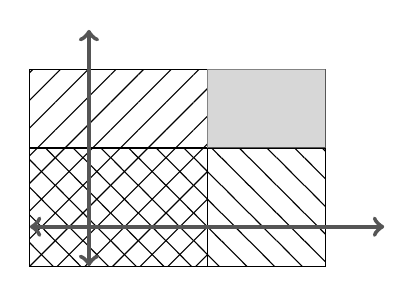
\begin{tikzpicture}[yscale=0.5, xscale=0.75]
  \coordinate (zzzz) at (-1,-1);
  \coordinate (a1zz) at ( 2,-1);
  \coordinate (zza2) at (-1, 2);
  \coordinate (b1zz) at ( 4,-1);
  \coordinate (zzb2) at (-1, 4);
  \coordinate (b1b2) at ( 4, 4);
  \coordinate (a1b2) at ( 2, 4);
  \coordinate (b1a2) at ( 4, 2);
  \coordinate (a1a2) at ( 2, 2);

  % Boxes
  \draw[] %
    (zzb2) -- (b1b2) -- (b1zz) -- (zzzz) -- (zzb2);
  \draw[pattern=my north west lines, line space=10pt] %
    (zza2) -- (b1a2) -- (b1zz) -- (zzzz) -- (zza2);
  \draw[pattern=my north east lines, line space=10pt] %
    (zzb2) -- (a1b2) -- (a1zz) -- (zzzz) -- (zzb2);
  \draw[color=d4gray, fill=d4gray, opacity=0.5] %
    (a1a2) -- (a1b2) -- (b1b2) -- (b1a2);

  % Axis
  \draw[d4black, ultra thick, <->] (-1,0) -- (5,0);
  \draw[d4black, ultra thick, <->] (0,-1) -- (0,5);
\end{tikzpicture}
\end{figure}
\end{rmk}

\begin{prop}
\emph{(CDF to $P$ on $(\R^n,\sB(\R)^{\otimes n})$)}
Given a function $F$ satisfying Definition~\ref{defn:F}, there exists a
unique probability measure $P$ on measurable space
$(\R^n,\sB(\R)^{\otimes n})$ such that
\begin{align*}
  P\big[\, (a_1,b_1]\times\cdots\times(a_n,b_n] \,\big] =
  \Delta_{a_1,b_2}
  \cdots
  \Delta_{a_n,b_n}
  F(x_1,\ldots,x_n)
  \qquad \forall \times_{k=1}^n (a_k,b_k]\in\sI_{(a,b]}^n
\end{align*}
\end{prop}


\clearpage
\subsection{Distribution of a Random Variable}
\label{sec:dist}

Having studied the connection between CDFs and probability measures on
$(\R,\sB(\R))$ (the range of RVs), we now examine how RVs link a
probability measure on their abstract measure-theoretic domain
$(\Omega,\sF)$ to a probability  measure on their range $(\R,\sB(\R))$,
the space we just studied.
In the process, this section clarifies how to compute probabilities and
expectations of RVs in practice with CDFs.


\begin{defn}(Probability Distribution of RV $X$)
\label{defn:probdist}
Suppose we have measure space $(\Omega,\sF,P)$ and RV
$X:(\Omega,\sF)\ra (\R,\sB(\R))$. From the probability measure $P$ on
the domain $(\Omega,\sF)$, we can construct the push forward
measure\footnote{%
  Definition~\ref{defn:pushfwd}
}
on the range $(\R,\sB(\R))$, denoted $P \circ X^{-1}$ or $P_X$ and
called the \emph{probability distribution of RV $X$}:
\begin{align*}
  P_X[A] =
  P\big[ X^{-1}(A) \big]
  \qquad \forall A\in\sB(\R)
\end{align*}
By Prop.~\ref{prop:ptocdf}, $P_X$ implies an associated (unique) CDF for
RV $X$:
\begin{align*}
  F_X(x)
  = P_X\big[(-\infty,x]\big]
  = P\big[X^{-1}\big((-\infty,x]\big)\big]
\end{align*}
\end{defn}

\begin{defn}(Classifying RVs)
We classify random vector
$X:(\Omega,\sF,P)\ra(\R^d,\sB(\R)^{\otimes d})$
by the Section~\ref{sec:abscts} classification of its distribution
$P_X=P\circ X^{-1}$.
So we call $X$
\begin{itemize}
  \item \emph{Discrete}: If $P_X$ is a discrete measure
  \item \emph{Continuous}: If $P_X$ is a continuous measure
  \item \emph{Absolutely Continuous}: If $P_X$ is an
    abs. continuous measure (permitting a density)
\end{itemize}
\end{defn}

\begin{prop}\emph{(Computing Expectation with $P_X$)}
\label{prop:expPX}
Given measure space $(\Omega,\sF,P)$, RV
$X:(\Omega,\sF)\ra (\R,\sB(\R))$  on that measure space, associated
prob. distribution $P_X$, and any measurable function
$g:(\R,\sB(\R))\ra(\R,\sB(\R))$, we can equivalently compute the
expectation
\begin{align}
  \E[g(X)]
  = \int_\Omega g \circ P \;dP
  = \int_\R g \;dP_X
  \label{expPX}
\end{align}
This is a change of variables that replaces integral of $g\circ X$ over
$(\Omega,\sF,P)$ with integral of $g$ over $(\R,\sB(\R),P_X)$.
\end{prop}
\begin{proof}
This follows directly from Proposition~\ref{prop:changeofvars}
about push forward measures.
\end{proof}

Expression~\ref{expPX} looks slightly better than the expression for the
expectation in our original Definition~\ref{defn:exp}. In particular,
we're now integrating over real measurable space $(\R,\sB(\R))$ rather
than super abstract measurable space $(\Omega,\sF)$. That's surely an
improvement, but we still don't necessarily know how to integrate with
respect to $P_X$ in practice. Therefore, we would like to replace
Expression~\ref{expPX} with a simple Riemman or Riemann-Stieltjes
integral over the PDF or CDF, rspectively, which we \emph{would}
definitely know how to compute.  The next few definitions and results
work towards that goal.

\begin{defn}(Right Quantile Function)
Given RV $X:(\Omega,\sF,P)\ra(\R,\sB(\R))$
with associated distribution $P_X$ and CDF $F_X$,
define the \emph{right quantile function}
\begin{align*}
  q_X:([0,1],\sB([0,1])\ra(\R,\sB(\R))
  \quad\text{where}\quad
  q_X(u) := \sup\{x\in\R\;|\; F_X(x)\leq u\}
\end{align*}
This is a real-valued measurable function, hence an RV with range
$(\R,\sB(\R))$.
\end{defn}

\begin{defn}(Prob. Measure of $q_X$)
\label{defn:probdistq}
If we use the Lebesgue measure $\lambda$ on its domain
$([0,1],\sB([0,1]))$, then by Definition~\ref{defn:probdist},
$q_X$ has prob. distribution on the range given by
\begin{align*}
  P_q[A] := \lambda[q_X^{-1}(A)]
  \qquad \forall A\in\sB(\R)
\end{align*}
\end{defn}


\begin{prop}\emph{($q_X$ and $X$ Have Same Distribution)}
\label{prop:equaldistqX}
Given RV $X:(\Omega,\sF)\ra(\R,\sB(\R))$ with associated
distribution $P_X$, CDF $F_X$, and right quantile function $q_X$,
\begin{align*}
  X \overset{d}{=} q_X
  \quad\iff\quad
  P_X[A] = P_q[A]
  \qquad \forall A\in\sB(\R)
\end{align*}
\end{prop}
\begin{proof}
We check that probability measures $P_X$ and $P_q$ agree on sets of the
form $(-\infty,x]$, in which case they agree on all of $\sB(\R)$ by
Proposition~\ref{prop:cdfunq}:
\begin{align*}
  P_q\big[(-\infty,x]\big]
  \underset{(1)}{=} \lambda[q_X \leq x]
  \underset{(2)}{=} \lambda[u\leq F_X(x)]
  \underset{(3)}{=} (F_X(x)- 0)
  \underset{(4)}{=} P_X\big[(-\infty,x]\big]
\end{align*}
Equality (1) is just Definition~\ref{defn:probdistq}.
Equality (2) follows from the definition of $q_X$.
Equality (3) is just computing Lebesgue measure of
$\{u\leq F_X(x)\}$.
Equality (4) is definition of $F_X$.
\end{proof}

\begin{thm}
\label{thm:expgX}
Given RV $X:(\Omega,\sF,P)\ra(\R,\sB(\R))$ with associated probability
distribution $P_X$ and CDF $F_X$,
\begin{align*}
  \E[g(X)]
  = \int_\Omega g\circ X \; dP
  = \int_\R g \; dP_X
  = \int_\R g \; dP_q
  = \int_{[0,1]} g \circ q_X \; d\lambda
  = \int_\R g  \; dF_X
  %\qquad
  %\forall \text{measurable} \; g:(\R,\sB(\R))\ra(\R,\sB(\R))
\end{align*}
The last integral in the chain is a Riemann-Stieltjes integral.
\end{thm}
\begin{proof}
First equal sign by Definition~\ref{defn:exp}.
Second and fourth equality by Proposition~\ref{prop:expPX}.
Third equality by Proposition~\ref{prop:equaldistqX}.
Final equality by?
\end{proof}

%How is all this stuff useful?
%Suppose we simply want to compute $\E[g(X)]$ for
%$g:(\R,\sB(\R))\ra(\R,\sB(\R))$.
%By the definition of expectations above, which uses only the probability
%measure $P$ on the domain, that means computing
%\begin{align*}
  %\E[g(X)] = \int_\Omega g\circ X\;dP
  %= \int_\Omega g(X(\omega))\; dP(d\omega)
  %%\qquad \forall g:(\R,\sB(\R))\ra (\R,\sB(\R))
%\end{align*}
%But \emph{alternatively}, I could integrate with respect to the
%\emph{distribution} of $X$. By its definition as the push-forward
%measure,
%\begin{align}
  %\E[g(X)]
  %= \int_\Omega g\circ X\;dP
  %= \int_\R g \; dP_X
  %\label{omega-Px}
%\end{align}

So that was a lot of work to justify computing the expectation of a
random variable with CDF $F_X$ via a Riemann-Stieltjes integral.  We had
to define the probability space $(\Omega,\sF,P)$, define the random
variable $X:(\Omega,\sF,P)\ra(\R,\sB(\R))$, compute its probability
distribution $P_X$, and link the integral with respect to this
distribution $P_X$ to a Riemann-Stieltjes integral with respect to its
CDF $F_X$.

Why did we do this? And how is it that we so easily and frequently
compute expectations and probabilities from CDFs \emph{in practice}
without \emph{ever} thinking about all this super-involved measure
theory?  The reason is that we \emph{invert} the steps described above.
Rather than start with super abstract $(\Omega,\sF,P)$ and move to
$X$, $P_X$, and $F_X$, we typically start by writing down the CDF $F_X$
\emph{directly}.  Then, we simply \emph{recognize} that it
implies a measure (unique by Proposition~\ref{prop:cdftop})
that can be \emph{interpreted} as the probability distribution
(push-forward measure) $P_X=P\circ X^{-1}$ of some RV $X$ on some
probability space $(\Omega,\sF,P)$.
Of course, there might be \emph{many} probability spaces and associated
RVs that imply this same CDF $F_X$.\footnote{%
  For example, the exponential distribution shows shows up so often
  precisely because there are many different real-world ``experiments''
  (all corresponding to different states/outcomes $\Omega$ and events
  $\sF$) which nonetheless imply exponentially distributed waiting
  times.
}
But in practice, that's fine. Really, we just care to know the CDF
itself (so we can compute expectations and probabilities) and
\emph{that there exists} an implicit measure-theory foundation
$(\Omega,\sF,P)$ and $X$ underlying everything.
But that implied measure theoretic structure is all pushed to the
background. In practice, we don't actually worry about it or work with
it really. But it's there for rigor's sake to justify computations
that we carry out with the CDF $F_X$.

\clearpage
\subsection{Independence}
\label{sec:independence}

\begin{defn}(Independence)
Let $(\Omega,\sF,P)$ be a probability space and let $J$ be a non-empty
indexing set. We define the following types of independence
\begin{enumerate}
  \item \emph{Events}: A family of events $\{A_\alpha\}_{\alpha\in J}$
    is independent if,
    for every finite sequence of distinct elements
    $\{i_1,\ldots,i_m\}\subseteq J$,
    \begin{align*}
      P[A_{i_1} \cap \cdots \cap A_{i_m}]
      = P[A_{i_1}]\times \cdots \times P[A_{i_m}]
    \end{align*}

  \item \emph{Family of $\sigma$-algebras}: Family of
    $\sigma$-algebras $\{\sF_\alpha\}_{\alpha\in J}$
    (where each $\sF_\alpha\subseteq \sF$ $\forall\alpha\in J$)
    is independent if the family of events
    $\{A_\alpha\}_{\alpha \in J}$ is independent where
    $A_{\alpha}\in \sF_{\alpha}$, $\alpha\in J$.

    In other words, construct the family of events
    $\{A_\alpha\}_{\alpha \in J}$ by plucking out some
    $A_\alpha \in \sF_\alpha\subseteq \sF$ for all $\alpha \in J$. The
    resulting family of events must be independent according to the
    first definition above for the family
    $\{\sF_\alpha\}_{\alpha \in J}$ to be independent.

  \item \emph{Random Variables}: A family of random variables
    $\{X_\alpha\}_{\alpha\in J}$ is independent if
    the family of $\sigma$-algebras
    $\{\sigma(X_\alpha)\}_{\alpha \in J}$ is independent.
\end{enumerate}
\end{defn}

\begin{prop}\emph{(Characterizations of Independence of Random Variables)}
\label{prop:indep}
Let $\{X_n\}\nN$ be a sequence of RVs on probability space
$(\Omega,\sF,P)$. Then the following are equivalent
\begin{enumerate}
  \item $X_1,\ldots,X_N$ independent (by the definition above)
  \item For all \textbf{bounded} Borel functions (i.e.
    $f_n:(\R,\sB(\R)) \ra (\R,\sB(\R))$ measurable),
    \begin{align}
      \E\left[\prod\nN f_n(X_n)\right]
      =
      \prod\nN \E\left[f_n(X_n)\right]
      \label{indepchar}
    \end{align}
  \item
    The joint characteristic function of
    $X := \begin{pmatrix} X_1 &\cdots & X_N \end{pmatrix}'$,
    equals the product of characteristic functions of the constituent
    $X_n$, i.e. for any $u\in \R^N$,
    \begin{align*}
      \E\left[e^{iu' X}\right]
      =
      \prod\nN \E\left[e^{iu_n X_n}\right]
    \end{align*}
\end{enumerate}
\begin{rmk}
One subtletly:
If $X_1,\ldots,X_N$ independent, Expression~\ref{indepchar} is true
\emph{regardless} of whether $\{f_n\}$ bounded---i.e.\
given independence, can \emph{always} factor expectation of a product
into product of expectations.

So why the ``bounded'' caveat? Characterization 2 says merely that it's
\emph{sufficient} to look at only bounded functions if you are
\emph{checking} independence. While independence \emph{implies}
Expression~\ref{indepchar} for any measurable $\{f_n\}\nN$
(bounded or not), it's \emph{enough} just to check
Expression~\ref{indepchar} for bounded functions to check
independence. You don't also have to check the expression
for unbounded functions.
\end{rmk}
\end{prop}
\begin{cor}
If $X,Y\in L^2$ independent, then
$\E[XY] = \E[X]\E[Y]$ hence
$\Corr[X,Y] = 0$.
\end{cor}
\begin{proof}
For fixed $m$, define
$X_m := \max\{\min\{X,m\}, -m\}$.
For each $m$, the statement should hold. Use Lebesgue's DCT.
\end{proof}

\clearpage
\subsection{Borel-Cantelli}

\begin{defn}(Limsup and Liminf of Events)
Given sequence of sets $\{A_n\}\ninf$, define the limsup and liminf of
events
\begin{align*}
  \limsup A_n := \bigcap\ninf \bigcup_{m \geq n} A_m
  \qquad
  \liminf A_n := \bigcup\ninf \bigcap_{m \geq n} A_m
\end{align*}
The limsup of sets contains those elements that ``show up infinitely
often'':
\begin{align*}
  x\in \limsup A_n
  \quad\implies\quad
  \forall N
  \;\; \exists m>N
  \;\; \text{s.t.}
  \;\; x\in A_m
\end{align*}
The liminf of sets contains those elements that ``show up in all sets,
with only finitely many exceptions at the beginning'':
\begin{align*}
  x\in \liminf A_n
  \quad\implies\quad
  \exists N
  \;\; \text{s.t.}\;\;
  x \in A_m
  \quad \forall m>N
\end{align*}
\end{defn}

\begin{lem}\emph{(Borel-Cantelli)}
Let $\{A_n\}\ninf\subseteq\sF$ be a sequence of events in probability
space $(\Omega,\sF,P)$. Then we have two results:
\begin{itemize}
  \item
    If the sum of probabilities of the infinite collection of events
    is finite, then the set of outcomes ocurring infinitely often must
    have probability zero:
    \begin{align*}
      \sumninf P(A_n) < \infty
      \quad\implies\quad
      P\left(\bigcap\ninf \bigcup_{m\geq n} A_n\right) = 0
    \end{align*}

  \item
    If the sum of probabilities of the infinite collection of
    independent events is finite, then the set of outcomes ocurring
    infinitely often must have probability one:
    \begin{align*}
      \begin{rcases}
        \{A_n\}\ninf \; \text{\emph{independent}}\\
        \sumninf P[A_n] = \infty
      \end{rcases}
      \quad\implies\quad
      P\left(\bigcap\ninf \bigcup_{m\geq n} A_n\right) = 1
    \end{align*}
\end{itemize}
\end{lem}

\clearpage
\subsection{Complex Random Variables}

\begin{prop}
Let $X\in\C^d$ be a $d$-dimensional complex random variable. Then
\begin{align*}
  \E[X] = \E[\Re(X)] + i\;\E[\Im(X)]
\end{align*}
\end{prop}

\begin{defn}
Let $Z = V+iW$, where $V$ and $W$ are real-valued integrable random
variables. Then we say that $Z$ is \emph{square integrable} if
$\E[|Z|^2]=\E[V^2 + W^2]<\infty$.
\end{defn}

\begin{prop}
Let $Z = V+iW$ and $Z' = V'+iW'$, where $V$, $W$, $V'$, and $W'$ are
real-valued integrable random variables. Then
\begin{enumerate}[label=\emph{(\roman*)}]
  \item $\E[Z] = \E[V] + i\E[W]$
  \item $\E[\,|Z|\,] = \E\left[\sqrt{V^2 + W^2}\right] \leq
    \E\big[|V|+|W|\big]<\infty$
  \item $\big|\E[Z]\big|\leq \E[\,|Z|\,]$
  \item $Z$ and $Z'$ are independent if $\sigma(V,W)$ is independent of
    $\sigma(V',W')$
  \item If $Z$ and $Z'$ are independent and square integrable, then
    $\E[Z\cdot Z'] = \E[Z]\cdot\E[Z']$
\end{enumerate}
\end{prop}
\begin{proof}
We prove each in turn:
\begin{enumerate}
  \item[(iii)]
    First, we want a clever way to write $\big|\E[Z]\big|$. To do so,
    make use of the following result:
    \begin{align}
      |z| = \sup_{q\in\Q} \Re(e^{iq}z)
      \qquad\forall z = v+iw\in\C
      \label{absvalz}
    \end{align}
    To prove this claim, we expand out the object on the RHS:
    \begin{align*}
      \Re(e^{iq}z)
      &= \Re\big(
      \left(\cos(q) + i\sin(q)\right)
      \cdot
      \left(v + iw\right)
      \big)
      =\cos(q)v - \sin(q)w
    \end{align*}
    Now we want the $q$ that maximizes this object. Since everything is
    differentiable, the first order necessary condition for an optimum
    is
    \begin{align*}
      0 &=-\sin(q)v - \cos(q)w
      \quad\implies\quad
      -\frac{w}{v} =
      \frac{\sin(q)}{\cos(q)} = \tan(q)
      \quad \implies\quad
      q = \arctan\left(-\frac{w}{v}\right)
    \end{align*}
    Using this in the expression for $\Re(e^{iq}z)$, we get
    \begin{align*}
      \sup_q
      \Re(e^{iq}z)
      &=
      \cos\left(\arctan\left(-\frac{w}{v}\right)\right)v -
      \sin\left(\arctan\left(-\frac{w}{v}\right)\right)w \\
      &=
      \frac{v}{\sqrt{1+\left(-\frac{w}{v}\right)^2}}
      -
      \frac{\left(-\frac{w}{v}\right)w}{\sqrt{1+\left(-\frac{w}{v}\right)^2}}
      \\
      &= \sqrt{v^2+w^2} \\
      \implies\quad
      \sup_q
      \Re(e^{iq}z)
      &= |z|
    \end{align*}
    We will be able to apply this to $\big|\E[Z]\big|$, since that's
    just a complex number in $\C$ like $z$ above. But first start by
    fixing $q\in\Q$ and use linearity of the expectation operator along
    with (i) to get
    \begin{align*}
      \Re\left(e^{iq}\E[Z]\right)
      &= \Re\left(\E[e^{iq}Z]\right)
      = \E\left[\Re(e^{iq}Z)\right]
    \end{align*}
    Now take the supremum over $q\in\Q$ on both sides to get
    \begin{align*}
      \sup_{q\in\Q}\Re\left(e^{iq}\E[Z]\right)
      &= \sup_{q\in\Q}\E\left[\Re(e^{iq}Z)\right] \\
      \text{By (\ref{absvalz})}\quad\implies\quad
      \big|\E[Z]\big|
      &= \sup_{q\in\Q}\E\left[\Re(e^{iq}Z)\right]
    \end{align*}
    Next, by Jensen since the supremum is a convex function, we get
    \begin{align*}
      \big|\E[Z]\big|
      &\leq \E\left[\sup_{q\in\Q}\Re(e^{iq}Z)\right] \\
      \text{By (\ref{absvalz}) again}\quad\implies\quad
      \big|\E[Z]\big|
      &\leq \E\left[\,|Z|\,\right]
    \end{align*}

\end{enumerate}
\end{proof}


\clearpage
\subsection{Characteristic Functions}

Characteristic functions are very useful.
They are the Fourier transform of the density,
give moments from derivatives, \emph{always} exist (even for
fat-tailed distributions, unlike MGFs), and \emph{uniquely} determine
distribution so that $X\dto Y$ equivalent to $\varphi_X \ra
\varphi_Y$ pointwise.

\begin{defn}(Characteristic Function)
Let $X$ be a $d$-dimensional random vector on probability space
$(\Omega,\sF,P)$ with CDF
$F_{X}(x_1,\ldots,x_d)
=
P_X[X_1\leq x_1,\ldots, X_d\leq x_d]$.
Then the \emph{characteristic function} $\varphi_X:\R^d\ra \C$ is
defined
\begin{align*}
  \varphi_X(u)
  &:= \int_{\R^d} e^{iu'X} \; dF_{X}
  = \E\left[e^{iu'X}\right] =
  \E\left[\cos(u'X)\right]+i\,\E\left[\sin(u'X)\right]
  %\quad\text{where}\quad u' X = \sum_{i=1}^d u_iX_i
\end{align*}
If $X$ absolutely continuous, it has density $f_{X}(x)=F'_X(x)$, and we
can write the characteristic function more explicitly as the Fourier
transform of the density:
\begin{align*}
  \varphi_X(u)
  &=
  \int_{\R^d} e^{iu'X} f_{X}(x)\; dx
\end{align*}
\end{defn}

\begin{prop}\emph{(Properties of Characteristic Functions)}
Given RV $X$ and associated $\varphi_X$
\begin{enumerate}[label=\emph{(\roman*)}]
  \item $|\varphi_X(u)| \leq \varphi_X(0) = 1$
  \item $\varphi_X(u) = \overline{\varphi_X(-u)}$
  \item $\varphi_X(u)$ is real-valued if and only if $X$ is symmetric,
    i.e. $X \overset{d}{=} -X$
  \item $\varphi_X(u)$ is uniformly continuous in $u$
\end{enumerate}
\end{prop}
\begin{proof}
We prove each in turn
\begin{enumerate}[label=(\roman*)]
  \item Recall for complex $Z$, $\big|\E[Z]\big|\leq \E[\,|Z|\,]$.
    Also, rather trivially, $\varphi_X(0)=\E[e^{0}] = 1$.
    Hence
    \begin{align*}
      |\varphi_X(u)|
      =
      \left\lvert\E\left[e^{iu'X}\right]\right\rvert
      &\leq
      \E\left[\left\lvert e^{iu'X}\right\rvert\right]
      = 1 = \varphi_X(0)
    \end{align*}

  \item Simply write out:
    $\overline{\varphi_X(-u)}
    =
    \overline{\E\left[e^{-iu'X}\right]}
    =
    \E\left[\,\overline{e^{-iu'X}}\,\right]
    =
    \E\left[e^{iu'X}\right]
    =
    \varphi_X(u)$

  \item
    ($\Rightarrow$)
    Suppose $\varphi_X(u)$ real-valued. To show $X$ symmetric, must show
    $-X$ has the same distribution, i.e. same characteristic function
    $\varphi_{-X}=\varphi_X$ by Theorem~\ref{cor:charfcnunq}. Start with
    \begin{align*}
      \varphi_{-X}(u)
      =
      \E\left[e^{-iu'X}\right]
      =
      \E\left[\overline{e^{iu'X}}\right]
      &=
      \overline{\E\left[e^{iu'X}\right]}
      =
      \overline{\varphi_X(u)}
      = \varphi_X(u)
    \end{align*}
    ($\Leftarrow$)
    Suppose $X$ symmetric so that $X\overset{d}{=}-X$. Then
    again, by Theorem~\ref{cor:charfcnunq},
    \begin{align}
      \varphi_X(u)&=\varphi_{-X}(u)
      \quad\iff\quad
      \E\left[e^{iu'X}\right]
      = \E\left[e^{-iu'X}\right]
      \label{charfcnsymmetric}
    \end{align}
    Then simplify by formula $\Im(z) = (z - \bar{z})/2i$
    and (\ref{charfcnsymmetric})
    \begin{align*}
      \Im(\varphi_X(u))
      &=
      \frac{\varphi_X(u)-\overline{\varphi_X(u)}}{2i}
      =
      \frac{\E\left[e^{iu'X}\right]-\E\left[e^{-iu'X}\right]}{2i}
      =
      0
      \;\implies\;
      \text{$\varphi_X(u)$ real-valued}
    \end{align*}

  \item For uniform continuity, we must be able to pick
    $\delta$ given $\varepsilon$ regardless of $u$. So consider
    \begin{align*}
      %\left\lvert
      %\varphi_X(u+\delta) - \varphi_X(u)
      %\right\rvert
      %=
      \bigg\lvert
        \underbrace{%
          \E\big[ e^{i(u'+\delta)X} - e^{iu'X} \big]
        }_{\varphi_X(u+\delta)-\varphi_X(u)}
      \bigg\rvert
      &\leq
      \E\bigg[
      \left\lvert
      e^{i\delta X}-1
      \right\rvert
      \cdot
      \underbrace{\left\lvert e^{iu'X} \right\rvert}_{\leq 1}
      \bigg]
      \leq
      \E\big[
      \left\lvert
      e^{i\delta X}-1
      \right\rvert
      \big]
    \end{align*}
    By Lebesgue's DCT, $|\varphi_X(u+\delta)-\varphi_X(u)|$
    goes to zero as $\delta\ra 0$ (regardless of $u$).
\end{enumerate}
\end{proof}

\begin{thm}\emph{(Moments from $\varphi_X$)}
\label{thm:charfcnmoments}
Let $X$ be an RV with associated $\varphi_X$.
Then
\begin{enumerate}[label=\emph{(\roman*)}]
  \item
    If $\E[|X|^n]<\infty$ for some $n\in\N_+$,
    then $\varphi_X^{(k)}(u)$ exists for all $k\leq n$ and
    \begin{align*}
      \varphi^{(k)}_X(u)
      = \E\big[(iX)^k e^{iu'X}\big]
      \quad\implies\quad
      \E\big[X^k\big]
      = (-i)^k \varphi^{(k)}_X(0)
    \end{align*}
  \item
    If $\varphi_X^{(2k)}(0)$ exists, then $\E[X^{2k}]<\infty$.
\end{enumerate}
These statements are roughly (but not quite exact) converses.
\end{thm}
\begin{proof}
We prove each in turn:
\begin{enumerate}[label=(\roman*)]
  \item
    Given $\E[|X|^n]<\infty$, Corollary~\ref{cor:jensen} implies
    $\E[|X|^k]<\infty$ for all $k\leq n$.
    Next, write out
    \begin{align*}
      \frac{\varphi_X(u+h)-\varphi_X(u)}{h}
      = \frac{\E[e^{i(u+h)X}-e^{iuX}]}{h}
      = \E\left[\frac{(e^{ihX}-1)e^{iuX}}{h}\right]
    \end{align*}
    Send $h\ra 0$.
    Since
    $\left\lvert\frac{(e^{ihX}-1)e^{iuX}}{h}\right\rvert<|X|\in L^1$,
    Lebesgue's DCT to take limit inside:
    \begin{align*}
      \lim_{h\ra 0}
      \frac{\varphi_X(u+h)-\varphi_X(u)}{h}
      %= \lim_{h\ra 0}
      %\E\left[\frac{(e^{ihX}-1)e^{iuX}}{h}\right]
      =
      \E\left[
      \lim_{h\ra 0}
      \frac{(e^{ihX}-1)e^{iuX}}{h}
      \right]
      =
      \E\left[(iX)e^{iuX}\right]
    \end{align*}
    Last equality from L'Hospital. Induction for $k>1$.

  \item
    Start with $k=1$. Since $\varphi^{(2)}_X(0)=\varphi_X''(0)$ exists,
    by derivative definitions/formulas,\footnote{%
      Among them, standard definitions
      $f'(x)
      := \lim_{h\ra 0} \frac{f(x+h)-f(x)}{h}
      = \lim_{h\ra 0} \frac{f(x)-f(x-h)}{h}$.
      Can also add both definitions together, cancel out $f(x)$ in
      the numerator, and get
      $2f'(x) = \lim_{h\ra 0}
      \left[
      \frac{f(x+h)-f(x-h)}{h}
      \right]$. Rearrange.
    }
    \begin{align*}
      \varphi_X''(0)
      &= \lim_{h\ra 0}
      \frac{1}{2}
      \;\left[
      \frac{\varphi_X'(2h)-\varphi_X'(-2h)}{2h}
      \right]
      %= \lim_{h\ra 0}
      %\frac{1}{4h}
      %\left[
      %\varphi_X'(2h)-\varphi_X'(-2h)
      %\right]
      \\
      &=
      \lim_{h\ra 0}
      \frac{1}{4h}
      \left[
      \lim_{h'\ra 0}
      \left[
      \frac{\varphi_X(2h)-\varphi_X(2h-2h')}{2h'}
      \right]
      -
      \lim_{h'\ra 0}
      \left[
      \frac{\varphi_X(-2h+2h')-\varphi_X(-2h)}{2h'}
      \right]
      \right]
    \end{align*}
    We can consolidate under a single limit $h\ra0$ and simplify to
    \begin{align*}
      \varphi_X''(0)
      &=
      \lim_{h\ra 0}
      \frac{\varphi_X(2h)-2\varphi_X(0)+\varphi_X(-2h)}{8h^2}
      \\
      &=
      \lim_{h\ra 0}
      \frac{%
        \E\left[
          e^{2ihX}
          + 2e^{0}
          + e^{-2ihX}
        \right]
      }{8h^2}
      =
      \lim_{h\ra 0}
      \frac{%
        \E\left[
          (e^{ihX} - e^{-ihX})^2
        \right]
      }{8h^2}
      \\
      &=
      \lim_{h\ra 0}
      -\frac{1}{2}
      \E\left[
      \left(
      \frac{\sin(hX)}{hX}
      \right)^2
      X^2
      \right]
      \\
      \text{Fatou}\quad
      &\leq
      -\frac{1}{2}
      \E\left[
      \lim_{h\ra 0}
      \left(
      \frac{\sin(hX)}{hX}
      \right)^2
      X^2
      \right]
      \\
      \text{L'Hospital}
      \;\implies
      \quad
      \varphi_X''(0)
      &\leq
      -\frac{1}{2}
      \E\left[
      \lim_{h\ra 0}
      \left(
      \frac{\cos(hX)X}{X}
      \right)^2
      X^2
      \right]
      =
      -\frac{1}{2}
      \E\left[
      X^2
      \right]
    \end{align*}
    Rearranging (and by assumed $\varphi''_X(0)<\infty$),
    we have the desired result for $k=1$:
    \begin{align*}
      \E\left[
      X^2
      \right]
      &\leq
      -2\varphi_X''(0) < \infty
    \end{align*}
    Now want to use induction to show the result for $k+1$ assuming $k$
    holds, i.e. assuming $\E[X^{2k}]=\E[|X|^{2k}]<\infty$.
    %Therefore, can apply Part (i) to $k$ case:
    %\begin{align*}
      %\varphi_X^{(2k)}(u)
      %= \E[(iX)^{2k} e^{iu'X}]
    %\end{align*}
    %If $P_X$ is the measure associated with $F_X$, define alternative
    %probability measure
    %$\tilde{P}_X$:
    %\begin{align*}
      %\tilde{P}_X[A]
      %:=
      %\frac{\E[\one{A} X^{2k}]}{\E[X^{2k}]}
      %\quad\implies\quad
      %\tilde{F}_X(x)
      %=
      %\frac{\E[\one{(-\infty,x]} X^{2k}]}{\E[X^{2k}]}
      %=
      %\frac{%
        %\int_{-\infty}^\infty \one{(-\infty,x]} x^{2k}\;dF(x)
      %}{\E[X^{2k}]}
      %=
      %\frac{%
        %\int_{-\infty}^x x^{2k}\;dF(x)
      %}{\E[X^{2k}]}
      %%=
      %%\frac{%
        %%\int_{-\infty}^x x^{2k}\;dF(x)
      %%}{\E[X^{2k}]}
    %\end{align*}
    %Then
    %\begin{align*}
      %\tilde{\varphi}_X(u)
      %= \tilde{\E}[e^{iuX}]
      %=
      %\int_{-\infty}^\infty
      %e^{iux}\;d\tilde{F}_X(x)
    %\end{align*}
\end{enumerate}
\end{proof}

\begin{cor}\emph{(Taylor Expansion for $\varphi_X$)}
\label{cor:chartaylor}
Given RV $X$ such that $\E[|X|^n]<\infty$ for some $n\in\N_+$,
we can express the associated characteristic function $\varphi_X$ as
\begin{align*}
  \varphi_X(u)
  = \sum_{k=0}^n
  \frac{(iu)^k}{k!}
  \E[X^k]
  + \frac{(iu)^n}{n!}\varepsilon_n(u)
  \quad\text{where}\;
  \lim_{u\ra 0}\varepsilon_n(u)=0
\end{align*}
\end{cor}
\begin{proof}
This is straightforward application of Taylor's Theorem to the function
$\varphi_X(u)$, expanding about $u=0$ and using
Theorem~\ref{thm:charfcnmoments} to replace derivatives
$\varphi_X^{(k)}(u)$ with moments.
\end{proof}


\begin{thm}\emph{(Inversion Formula)}
Given RV $X$ with CDF and c.f. $F_X$ and $\varphi_X$,
\begin{enumerate}[label=\emph{(\roman*)}]
  \item
    (\emph{$\varphi_X$ \emph{uniquely} determines probabilities}):
    \begin{align*}
      \frac{F(b) + F(b^-)}{2}
      - \frac{F(a) + F(a^-)}{2}
      = \lim_{c\ra\infty}
      \frac{1}{2\pi}
      \int^c_{-c}
      \frac{e^{-ita}-e^{-itb}}{it}
      \varphi_X(t) \; dt
    \end{align*}
  \item
    \emph{(Can use $\varphi_X$ to test whether density exists)}:
    If $\int_\R |\varphi_X(u)|\;du<\infty$, then $F$ has has a
    continuous density function
    \begin{align*}
      f(x) = \frac{1}{2\pi}\int_{-\infty}^\infty
      e^{-itx}\varphi_X(t)\;dt
    \end{align*}
\end{enumerate}
\end{thm}
\begin{rmk}
To understand the LHS in (i), consider $b$.
Since $F$ necessarily right continuous, $F(b^+)=F(b)$. However,
$F$ is not necessarily continuous, so it's possible that
$F(b^+)=F(b)\neq F(b^-)$. In that case, the LHS uses the midpoint of
the discontinuity at $b$. Lastly, if $F$ continuous, the LHS
reduces to simply $F(b)-F(a)$.
\end{rmk}

\begin{cor}
\label{cor:charfcnunq}
\emph{($\varphi_X$ Uniquely Characterizes Distribution of $X$)}
The distribution of RV $X$ is uniquely determined by its characteristic
function $\varphi_X$.
\end{cor}

\begin{thm}\emph{(Continuity Theorem)}
Let $\{X_n\}$ be a sequence of RVs on sequence of probability spaces
$(\Omega_n,\sF_n,P_n)$ with corresponding characteristic functions
$\varphi_n(u) = \E[e^{iuX_n}]$.
\begin{enumerate}[label=\emph{(\roman*)}]
  \item If $X_n\dto X$ for some RV $X$ on a probability space
    $(\Omega,\sF,P)$ with associated characteristic function
    $\varphi(u)$, then we have convergence of characteristic
    functions $\varphi_n(u)\ra \varphi(u)$ pointwise
    for all $u$.
  \item
    If there exists a function $\varphi(u)$ continuous at $u=0$ such
    that $\varphi_n(u)\ra\varphi(u)$ pointwise for all $u$,
    then $\varphi(u)$ is the c.f. of some
    corresponding RV $X$ and $X_n\dto X$.
\end{enumerate}
\end{thm}

\begin{thm}\emph{(Central Limit Theorem)}
Let $\{X_n\}\ninf$ be a sequence of iid RVs
on probability space $(\Omega,\sF,P)$ such that
$\E[X^2_n]<\infty$ and $\sigma^2=\Var(X_n)>0$.
Then
\begin{align*}
  \frac{1}{\sqrt{N}}
  \sumnN \frac{X_n-\E[X_n]}{\sigma}
  \dto \calN(0,1)
\end{align*}
\end{thm}
\begin{proof}
Define the normalization
\begin{align*}
  Y_n := \frac{X_n-\E[X_n]}{\sigma}
  \quad\implies\quad
  \E[Y_n] = 0,\;\text{and}\;\;
  \E[Y_n^2] = 1
  \qquad\forall n
\end{align*}
By Corollary~\ref{cor:chartaylor} up to order 2 (since we assumed only
that $\E[X^2_n]<\infty$),
\begin{align*}
  \varphi_Y(u)
  &=
  \sum_{k=0}^2
  \frac{(iu)^k}{k!}
  \E[Y^k]
  - \frac{u^2}{2}\varepsilon_2(u)
  =
  1 + (iu)\E[Y]
  - \frac{u^2}{2} \E[Y^2]
  - \frac{u^2}{2}\varepsilon_2(u)
  \\
  &=
  1
  - \frac{u^2}{2}
  - \frac{u^2}{2}\varepsilon_2(u)
  \qquad\text{where}\;
  \lim_{u\ra 0}\varepsilon_2(u)=0
  \\
  \varphi_{Y/\sqrt{N}}(u)
  &=
  1
  - \frac{u^2}{2N}
  - \frac{u^2}{2N}\varepsilon_2(u)
\end{align*}
Write out
\begin{align*}
  \varphi_n(u)
  :=
  \E[e^{iuY_n}]
  =
\end{align*}
\end{proof}


\clearpage
\subsection{Conditional Expectation and Probability}

\begin{defn}(Conditional Expectation)
Let $(\Omega,\sF,P)$ be a probability space and $X\in L^1(\Omega,\sF,P)$
with $\sG\subseteq\sF$ a sub-$\sigma$-algebra. Define the
\emph{conditional expectation} $Y=\E[X|\sG]$ as a random variable such
that
\begin{align*}
  \E[\one{A}Y] = \E[\one{A}X]
  \qquad \forall A\in \sG
\end{align*}
If $Z$ is another random variable on $(\Omega,\sF,P)$, then we use the
shorthand
\begin{align*}
  \E[X|Z]
  \quad\iff\quad
  \E[X|\sigma(Z)]
\end{align*}
with the former being the shorthand notation and the latter expression
representing the most precise meaning (since the conditional
expectation is only defined for a $\sigma$-algebra).
\end{defn}

\begin{prop}
The conditional expectation \emph{exists} and is \emph{unique} up to
$P$-a.e.\ equality for any $X\in L^1(\Omega,\sF,P)$.
\end{prop}

\begin{defn}(Conditional Probability)
Given probability space $(\Omega,\sF,P)$, event $A\in\sF$, and
sub-$\sigma$-algebra $\sG\subseteq\sF$, define
\begin{align*}
  P[A|\sG] := \E[\one{A}|\sG]
\end{align*}
\end{defn}

\begin{prop}\emph{(Properties of the Conditional Expectation)}
Let $(\Omega,\sF,P)$ be a probability space and
$X,Y\in L^1(\Omega,\sF,P)$ with $\sG\subseteq\sF$ a
sub-$\sigma$-algebra. Then
\begin{enumerate}[label=(\roman*)]
  \item If $X$ is $\sG$ measurable, then $\E[X|\sG]=X$.
  \item Tower Property: For any sub-$\sigma$-algebra $\sH\subseteq\sG$,
    we have
    \begin{align*}
      \E\big[
        \,\E[X|\sG]\,
        \big|
        \sH
      \big]
      = \E[X|\sH]
    \end{align*}

  \item For $X$ independent of $\sG$, we have $\E[X|\sG]=\E[X]$.

  \item $X \geq Y$ $P$-a.s. implies that $\E[X|\sG]\geq\E[Y|\sG]$
    $P$-a.s.
  \item Conditional Jensen: For a convex function $\varphi:\R\ra \R$ suh
    such that $\varphi(X)\in L^1$, we have
    \begin{align*}
      \E[ \varphi(X) |\sG]
      \geq \varphi\left(\E[X|\sG]\right)
      \quad \text{a.s.}
    \end{align*}
    For a concave function, the inequality flips.

  \item $\lVert X\rVert_p\geq \lVert\,\E[X|\sG]\,\rVert_p$ (conditional
    expectation can only decrease in $p$-norm relative to the original
    $X$).
\end{enumerate}
\end{prop}
\begin{proof}
We prove each in turn
\begin{enumerate}[label=(\roman*)]
  \item
  \item
  \item Here, we can apply conditional Jensen since $|\,\cdot\,|^p$ is
    a convex function so that
    \begin{align*}
      \E[\lvert X\rvert^p\,|\,\sG]
      &\geq
      \big\lvert\,\E[X|\sG]\,\big\rvert^p
    \end{align*}
    Now take the uconditional expectation of each side:
    \begin{align*}
      \E\big[
      \E[\lvert X\rvert^p\,|\,\sG]
      \big]
      &\geq
      \E\big[
      \lvert\,\E[X|\sG]\,\rvert^p
      \big] \\
      \iff\quad
      \E\left[ \lvert X\rvert^p\right]
      &\geq
      \E\big[
      \lvert\,\E[X|\sG]\,\rvert^p
      \big]
    \end{align*}
    But then raise each side to the power $1/p$ and recongnize that
    \begin{align*}
      \E\left[ \lvert X\rvert^p\right]^{\frac{1}{p}}
      &\geq
      \E\big[
      \lvert\,\E[X|\sG]\,\rvert^p
      \big]^{\frac{1}{p}} \\
      \iff\quad
      \lVert X \rVert_p
      &\geq
      \lVert \, \E[X|\sG] \,\rVert_p
    \end{align*}
\end{enumerate}
\end{proof}

\begin{defn}
Let $X$ be a $\bar{\R}$-valued random variable on $(\Omega,\sF,P)$ and
let $\sG\subseteq \sF$ be a sub-$\sigma$-algebra. Then
\begin{enumerate}[label=(\roman*)]
  \item $\E[X^-]<\infty$, define
    \begin{align*}
      \E[X|\sG] = \limn \E[X\wedge n|\sG]
    \end{align*}
  \item $\E[X^+]<\infty$, define
    \begin{align*}
      \E[X|\sG] = \lim_{n\ra-\infty} \E[X\vee n|\sG]
    \end{align*}
\end{enumerate}
\end{defn}


\clearpage
\subsection{Transformation Theory}

In this section, we derive the distribution for some RV
$Y = g(X_1, \ldots, X_N)\in\R^N$
that is a function of $N$ other RVs (not necessarily iid),
$X_1,\ldots,X_N$.
We care about such $Y$ constructed/transformed from other RVs because
often
\begin{enumerate}
  \item We want to build up a more complex RV $Y$ by transforming
    relatively simple ones
  \item Maximum likelihood estimators are functions of data
    sample $\{X_n\}\nN$.
  \item Many test statistics are \emph{derived} statistics dependent on
    RVs $\{X_n\}\nN$.
\end{enumerate}
So we'll want the distribution of $Y\in\R^N$.
Throughout this subsection, we only consider absolutely continuous
random variables $\{X_n\}\nN$, i.e. RVs that permit a density.

\begin{thm}\emph{(Monotonic $g$, $N=1$)}
Suppose RV $X$ has density function $f_X(x)$ and $Y=g(X)$
for differentiable, \emph{monotonic} $g$. Then
\begin{align*}
   f_Y(y) &= \left[f_X(x) \left\lvert \frac{dx}{dy}\right\rvert
      \right]_{x = g^{-1}(y)}
    = \left[ f_X(x) \left\lvert \frac{dy}{dx}\right\rvert^{-1}
      \right]_{x = g^{-1}(y)}
\end{align*}
\end{thm}

\begin{thm}\emph{(Non-Monotonic $g$, $N=1$)}
Suppose RV $X$ has density $f_X(x)$ and $Y=g(X)$
for differentiable, \emph{non-monotonic} $g$. Then split up $g$ into
monotonic segments, denoted $g_1,\ldots,g_M$. Then
\begin{align}
   \label{nonmontrans}
   f_Y(y)
   &= \sum_{m=1}^M \left[ f_X(x_m) \left\lvert \frac{dx_m}{dy}
      \right\rvert \right]_{x_m=g_m^{-1}(y)}
   = \sum_{m=1}^M \left[ f_X(x_m) \left\lvert \frac{dy}{dx_m}
    \right\rvert^{-1} \right]_{x_m=g_m^{-1}(y)}
    \notag
\end{align}
\end{thm}

\begin{thm}\emph{(Invertible $g$, $N>1$)}
\label{thm:transformmultivar}
Given RV $X\in\R^N$ with jdf $f_{X}(x)$ and $Y=g(X)\in\R^N$
for some invertible function $g:\Rn\ra\Rn$.\footnote{%
  The invertibility assumption is similar to the monotonicity assumption
  in the $N=1$ case.
},
the jdf for vector $Y\in\R^N$ is given by
\begin{align*}
  f_{Y}(y)
  %&= \left[ f_{X}(x) \lvert J \rvert \right]_{x=g^{-1}(y)} \\
   &= \left[
      f_{X}(x)\frac{1}{\lvert J\rvert}
      \right]_{x=g^{-1}(y)}
  \qquad\text{where}\quad
  |J| =\det
   %J = \begin{bmatrix} \frac{\partial x_1}{\partial y_1} &
      %\frac{\partial x_1}{\partial y_2} & \cdots &
      %\frac{\partial x_1}{\partial y_n} \\
      %\vdots & & \ddots & \vdots \\
      %\frac{\partial x_n}{\partial y_1} &
      %\frac{\partial x_n}{\partial y_2} & \cdots &
      %\frac{\partial x_n}{\partial y_n}
   %\end{bmatrix} \qquad \qquad
   %J =
   \begin{bmatrix} \frac{\partial g_1}{\partial x_1} &
      \frac{\partial g_1}{\partial x_2} & \cdots &
      \frac{\partial g_1}{\partial x_n} \\
      \vdots & & \ddots & \vdots \\
      \frac{\partial g_n}{\partial x_1} &
      \frac{\partial g_n}{\partial x_2} & \cdots &
      \frac{\partial g_n}{\partial x_n}
   \end{bmatrix}
\end{align*}
where $\frac{\partial g_i}{\partial x_j}$ is the partial derivative of
the $i$th element of $Y=g(X)$ with respect to the $j$th element of
vector $X$.
\end{thm}

\begin{rmk}
Often, we will even use this to do transformations that are not
1-to-1. That will involve doing a transformation that \emph{is}
1-to-1 using this method with dummy variables, then integrating
out those dummy variables.
\end{rmk}



\clearpage
\section{Select RVs and Stochastic Processes}

\subsection{Point Mass}

\begin{defn}(Point Mass)
Suppose we have RV $X\in\R^d$ with $P[X=x]=1$ for some $x\in\R^d$.
Then its characteristic function is given by
\begin{align*}
  \varphi_X(u)
  = \E[e^{iu'X}] = e^{iu'x}
\end{align*}
\end{defn}


\subsection{Gamma, Exponential, Poisson}

\begin{defn}(Gamma RV)
The Gamma($\alpha,\beta$) RV is that which has density
\begin{equation}
   f_X(x) = \frac{\beta^\alpha}{\Gamma(\alpha)} x^{\alpha-1}
    e^{-\beta x}, \quad x > 0
    \quad\implies\quad
    \text{Mean} = \frac{\alpha}{\beta}
    \quad
    \text{Variance} = \frac{\alpha}{\beta^2}
\end{equation}
\end{defn}

\begin{prop}\emph{(Sums of Gamma RVs are Gamma)}
Gamma RVs also satisfy
\begin{align*}
  X_n \sim \operatorname{Gamma}(\alpha_n, \;\beta)
  \quad \Rightarrow \quad
   \sumnN X_n \sim
   \operatorname{Gamma}\left(\sumnN \alpha_n,\;\beta \right)
\end{align*}
\end{prop}

\begin{defn}(Exponential RV)
An \emph{exponential} RV is a special case of the Gamma RV:
\begin{align*}
  \text{Exp}(\lambda)
  :=
  \text{Gamma}(1,\lambda)
  \quad\implies\quad
  f_X(x) = \lambda\; e^{-\lambda}
\end{align*}
This is a \emph{memoryless} distribution particularly useful for
waiting times.
CDF and moments are
\begin{align*}
  F_X(x)
  = 1 - e^{-\lambda x}
  \qquad
  \text{Mean} = \frac{1}{\lambda}
  \qquad
  \text{Variance} = \frac{1}{\lambda^2}
\end{align*}
\end{defn}

\begin{prop}\emph{(Sums of Exponential are Gamma)}
Given iid exponential RVs $\{X_n\}\nN$,
\begin{align*}
  X_n \sim \operatorname{Exp}(\lambda)
  \quad\implies\quad
  \sumnN X_n \sim \operatorname{Gamma}(N, \lambda)
\end{align*}
\end{prop}

\begin{defn}(Poisson Process)
We construct the continuous time \emph{Poisson process} with constant
parameter $\lambda$, denoted $N_t$, by building up from exponentially
distributed jump times:
\begin{itemize}
  \item $S_n\iid \operatorname{Exp}(\lambda)$:
    Time between $(n-1)$th and $n$th jump
  \item $T_N:=\sumnN S_n$ for $N\geq 0$:
    Time until $N$th jump, with $T_0:=0$
  \item $N_t:=\sum_{n\geq 0} \one{\{T_n\leq t\}}$
\end{itemize}
This implies that, for fixed $t$,
$N_t\sim\operatorname{Poisson}(\lambda t)$.
\end{defn}


\clearpage
\subsection{Normal or Gaussian}

\subsubsection{Univariate Normal/Gaussian Distribution}

\begin{defn}(Normal RV)
  \label{defn:stdnormal}
The \emph{standard normal} RV $Z\sim \calN(0,1)$ is that with density
\begin{align*}
   f_Z(z)
   = \frac{1}{\sqrt{2\pi}} \; e^{-\frac{1}{2}z^2}
\end{align*}
The \emph{general normal} RV $Y\sim\calN(\mu,\sigma^2)$ is defined
simply as
\begin{align*}
  Y := \mu + \sigma Z
  \quad\implies\quad
   f_Y(y) =
   \frac{1}{\sigma \sqrt{2\pi}}
   \; e^{-\frac{1}{2\sigma^2} (y - \mu)^2}
\end{align*}
\end{defn}
\begin{proof}
To prove that the above density $f_Y(y)$ is correct given definition
$Y:=\mu+\sigma Z$, compute the CDF of $Z$, shift and normalize to get
the CDF of $Y$, then differentiate.
\end{proof}

\begin{lem}\emph{(Integral of Exponentials)}
\label{lem:normintegral}
Handy integral result for working with normal RVs:
\begin{align}
  \frac{1}{\sqrt{2\pi}}
  \int_\R e^{az} e^{-\frac{1}{2}z^2}\; dz
  =
  e^{\frac{1}{2}a^2}
  %\label{eq:normintegral}
\end{align}
\end{lem}
\begin{proof}
To compute this integral (ignoring the constant), just complete the
square:
\begin{align*}
  \int_\R e^{az} e^{-\frac{1}{2}z^2}\; dz
  =
  \int_\R e^{-\frac{1}{2}\left(z^2-2az\right)}\; dz
  =
  \int_\R e^{-\frac{1}{2}\left(z^2-2az+a^2-a^2\right)}\; dz
  =
  e^{\frac{a^2}{2}}
  \int_\R e^{-\frac{1}{2}\left(z-a\right)^2}\; dz
\end{align*}
But the final integral in the chain is simply the integral of the
density of a $N(a,1)$ RV (without the multiplying constant).
Therefore, it equals $\sqrt{2\pi}$, implying
Result~\ref{lem:normintegral}.
\end{proof}

\begin{prop}\emph{(Characteristic Functions $\varphi_Z$, $\varphi_Y$)}
Characteristic functions of $Z$ and $Y$:
\begin{align*}
  \varphi_Z(u)
  = \E[e^{iuZ}]
  = e^{-\frac{1}{2}u^2}
  \qquad
  \varphi_Y(u)
  = \E[e^{iuY}]
  = e^{iu\mu-\frac{1}{2}(\sigma u)^2}
\end{align*}
\end{prop}
\begin{rmk}
Notice that as $\sigma\ra 0$, the characteristic function $\varphi_Y$
converges to the characteristic function of a point mass at $\mu$, i.e.
$Y$ converges in distribution to a point mass at $\mu$.
\end{rmk}
\begin{proof}
Use the density to compute the following function of $y$:
\begin{align*}
  \E[e^{aZ}]
  := \int_\R e^{az} f_Z(z) \; dz
  =
  \frac{1}{\sqrt{2\pi}}
  \int_\R e^{az} e^{-\frac{1}{2}z^2} \; dz
  = e^{\frac{1}{2}a^2}
\end{align*}
where the last result came from Lemma~\ref{lem:normintegral}.
Plug in $a=iu$ (which we can do by analytic continuity and complex
analysis) to get $\varphi_Z$.
Lastly, write out definition of $\varphi_Y(u)$:
\begin{align*}
  \varphi_Y(u)
  := \E[e^{iuY}]
  = \E[e^{iu(\mu+\sigma Z)}]
  = e^{iu\mu}\E[e^{iu\sigma Z}]
  = e^{iu\mu}\varphi_Z(\sigma u)
\end{align*}
\end{proof}

\clearpage
\subsubsection{Multivariate Normal}

\begin{defn}(Multivariate Normal)
\label{defn:mvn}
$d$-dimensional random vector $X$ is called \emph{multivariate normal}
or \emph{Gaussian} if it has characteristic function
\begin{align*}
  \varphi_X(u)
  = \E[e^{iu'X}]
  = e^{iu'\mu-\frac{1}{2}u'\Sigma u}
  \quad\text{for some}\quad
  \mu\in\R^d,\;\Sigma\in\R^{d\times d}
\end{align*}
where $\Sigma$ symmetric positive-semidefinite.
Denote by $X\sim\calN_d(\mu,\Sigma)$.
Further classify $X$
\begin{itemize}
  \item \emph{Regular} if $\Sigma$ \emph{invertible}, hence
    positive definite
  \item \emph{Degenerate} if $\Sigma$ \emph{not invertible},
    so positive \emph{semi}definite only.
    $X$ lives on subspace of $\R^d$.
\end{itemize}
\end{defn}

\begin{prop}\emph{(Construction of $Z=\calN_d(0,I_d)$ Density)}
The following function gives the density of a standard multivariate
normal random vector $Z\sim \calN_d(0,I_d)$.
\begin{align}
  f_Z(z_1,\ldots,z_d)
  = f_Z(z_1)\cdots f_Z(z_d)
  %=
  %\frac{1}{(2\pi)^{d/2}}
  %e^{-\frac{1}{2}\sum_{i=1}^d z_i^2}
  =
  \frac{1}{(2\pi)^{d/2}}
  e^{-\frac{1}{2}z'I_dz}
  \label{prop:mvndens}
\end{align}
\end{prop}
\begin{proof}
Expr.~\ref{prop:mvndens} is a product of univariate
densities $f_Z(z)$ on $(\R,\sB(\R))$.
Hence by Prop.~\ref{prop:densityproduct},
Expr.~\ref{prop:mvndens} is a density
%on $(\R,\sB(\R)^{\otimes d})$
corresponding to some measure/distribution $P_Z$ on
$(\R,\sB(\R)^{\otimes d})$ corresponding to a random vector $Z$ with
independent $\calN(0,1)$ components.
Hence, CF is
\begin{align*}
  \varphi_Z(u)
  := \E[e^{iu'Z}]
  \underset{(a)}{=}
    \E[e^{iu_1Z_1}]
    \cdots
    \E[e^{iu_dZ_d}]
  \underset{(b)}{=}
  \varphi_Z(u_1)\cdots\varphi_Z(u_d)
  \underset{(c)}{=}
  e^{-\frac{1}{2}u'I_du}
\end{align*}
(a) by independence of the $d$ components.
(b) since each component $\calN(0,1)$, hence each expectation is
precisely the definition of $\varphi_Z$.
(c) by subbing in expression for $\varphi_Z$ and simplifying.
Lastly, the final expression is the Definition~\ref{defn:mvn}
CF of a $\calN_d(0,I_d)$ RV.
Therefore, Expression~\ref{prop:mvndens} is precisely the density
associated with some $\calN_d(0,I_d)$-distributed RV $X$.
\end{proof}

\begin{prop}
Given vector $\mu\in\R^d$ and symmetric positive semi-definite
$\Sigma\in\R^{d\times d}$.
Define $Y:=\mu+LZ$ where $Z\sim\calN_d(0,I_d)$ and
$\Sigma=LL'$ is the Cholesky decomposition of $\Sigma$.\footnote{%
  Such a decomposition exists precisely because $\Sigma$ assumed
  symmetric positive semi-definite, though only unique if $\Sigma$
  positive definite. But regardless, such a decomposition exists, and
  that's all that matters.
}
\begin{enumerate}[label=\emph{(\roman*)}]
  \item $Y:=\mu+LZ\sim\calN_d(\mu,\Sigma)$.
  \item All components are mutually independent if and only if
    $\Cov(Y_i,Y_j)=0$ for all $i\neq j$
  \item If $\Sigma$ invertible (hence $\Sigma$ positive definite), then
    $Y$ has density
    \begin{equation}
      \label{pdf2}
      f_{Y}(y) =
      \frac{1}{(2\pi)^{d/2}\lvert \Sigma \rvert^{1/2}}
      \; e^{%
            -\frac{1}{2} (y-\mu)^T \; \Sigma^{-1} (y-\mu)
      }
      \qquad\text{where}\quad
      \lvert\Sigma\rvert = \det\Sigma,\quad y\in\R^d
    \end{equation}
  \item If $\Sigma$ not invertible, $Y$ lies in a strict subspace
    of $\R^d$ and cannot have a density on $\R^d$
  \item
    For every $\nu\in\R^k$ and $M\in\R^{k\times d}$
    $X:=\nu + MY \sim \calN_d(\nu + M\mu,\; M\Sigma M^T)$
\end{enumerate}
\end{prop}
\begin{proof}
We prove each in turn
\begin{enumerate}[label=(\roman*)]
  \item
    %Clearly $\E[Y]=\mu$. Now check
    %$\Cov(Y)=\Cov(\mu+LZ)=L\Cov(Z)L'=LI_dL'=\Sigma$.
    %That shows the moments are correct. Now let's
    We can check that the distribution of $Y$ is correct by checking the
    characteristic function:
    \begin{align*}
      \varphi_Y(u)
      := \E[e^{iu'Y}]
      = \E[e^{iu'(\mu+LZ)}]
      = e^{iu'\mu}\E[e^{iv'Z}]
      \qquad\text{where} \quad:=L'u
    \end{align*}
    But identify this last expectation as simply the definition of
    $\varphi_Z(v)$. Hence
    \begin{align*}
      \varphi_Y(u)
      = e^{iu'\mu}\varphi_Z(v)
      = e^{iu'\mu}e^{-\frac{1}{2}v'I_dv}
      = e^{iu'\mu-\frac{1}{2}u'\Sigma u}
    \end{align*}
    where we used the fact that $\Sigma=LL'$ is the Cholesky
    decomposition of $\Sigma$ to simplify $v'I_dv=u'LI_dL'u=u'\Sigma u$.
    And this last expression is precisely Definition~\ref{defn:mvn}.

  \item
    ($\Rightarrow$) is true for any random vector.
    ($\Leftarrow$) is a special result for normal RVs that is not
    generally true.
    To prove this direction, recall Proposition~\ref{prop:indep} which
    says that
    \begin{align*}
      Y_1,\ldots,Y_d \;\; \text{independent}
      \quad\iff\quad
      \varphi_Y(u) = \prod_{i=1}^d\varphi_{Y_i}(u_i)
    \end{align*}
    Now recall the Definition~\ref{defn:mvn} expression for
    $\varphi_Y(u)$
    \begin{align*}
      \varphi_Y(u)
      &= e^{iu'\mu-\frac{1}{2}u'\Sigma u}
      = \exp\left\{
          i\sum_{j=1}^du_j\mu_j
          -\frac{1}{2}\sum_{j=1}^d\sum_{k=1}^du_j\Sigma_{ij}u_k
        \right\}
    \end{align*}
    We can factor this into a product of univariate normal
    characteristic functions (implying independence), if and only if
    $\Sigma_{ij}=0$ for all $i\neq j$.

  \item
    We can use Theorem~\ref{thm:transformmultivar} on the
    transformation $Y=\mu+LZ$ and density $f_Z(z)$ in
    Expression~\ref{prop:mvndens}
    \begin{align*}
      f_{Y}(y)
      &= \left[
          f_{Z}(z)\frac{1}{\lvert J\rvert}
        \right]_{z=L^{-1}(y-\mu)}
      \qquad\text{where}\quad
      |J|
      = \det\left(\partial Y/\partial Z\right)
      = \det(L')
      \\
      &=
        \frac{1}{(2\pi)^{d/2}}
        e^{-\frac{1}{2}(y-\mu)'(L^{-1})' L^{-1}(y-\mu)}
        \frac{1}{\det(L')}
    \end{align*}
    Lastly, recall $\Sigma=LL'$ is invertible, $L$ triangular.
    Hence $0\neq\det(\Sigma)=\det(L)\det(L')=\det(L)^2$
    and $(L^{-1})'=(L')^{-1}$. Using these results,
    in the density expression above,
    \begin{align*}
      f_{Y}(y)
      &=
      \frac{1}{(2\pi)^{d/2}\sqrt{|\Sigma|}}
      e^{-\frac{1}{2}(y-\mu)'\Sigma^{-1} (y-\mu)}
    \end{align*}
  \item
    $\Sigma$ not invertible iff $L$ not invertible, which implies
    $L\R^d$ is a strict subspace of $\R^d$ and $\lambda(A\R^d)=0$, where
    $\lambda$ is the Lebesgue measure.
  \item
    Simply compute the characteristic function of $X=\nu+MY$.
    \begin{align*}
      \varphi_X(u)
      = \E[e^{iu'X}]
      = \E[e^{iu'(\nu+MY)}]
      = e^{iu'\nu}\E[e^{i(M'u)'Y}]
      = e^{iu'\nu}\varphi_Y(M'u)
      = e^{iu'(\nu+M\mu)-\frac{1}{2}u'M\Sigma M'u}
    \end{align*}
\end{enumerate}
\end{proof}

\clearpage
\begin{prop}
$X\sim \calN_d(\mu,\Sigma)$ if and only if $v'X$ is univariate normal
for all $v\in\R^d$.
\end{prop}
\begin{proof}
($\Rightarrow$)
Start by computing the characteristic function $\varphi_{v'X}(u)$ where
$u$ is a scalar:
\begin{align*}
  \varphi_{v'X}(u)
  = \E[e^{iu(v'X)}]
  = \E[e^{iuv'X}]
  = \varphi_X(uv)
\end{align*}
where $\varphi_X(\tilde{u})$ is the characteristic function of $X$.
Since $X\sim\calN_d(\mu,\Sigma)$, CF $\varphi_X(\tilde{u})$ is given by
Definition~\ref{defn:mvn}, hence
\begin{align*}
  \varphi_{v'X}(u)
  = \varphi_X(uv)
  = e^{i(uv)'\mu-\frac{1}{2}(uv)'\Sigma(uv)}
  = e^{iu(v'\mu)-\frac{1}{2}u(v'\Sigma v)u}
\end{align*}
which implies precisely that $v'X$ univariate normal,
$v'X\sim\calN(v'\mu,v'\Sigma v)$

($\Leftarrow$)
If $v'X$ is normal for all $v\in\R^d$, then vector $X$ is square
integrable, so $\mu:=\E[X]$ and $\Sigma:=\Cov(X)$ exist and
well-defined.
Just need to show $X$ $\calN_d(\mu,\Sigma)$, which we do by showing that
it has the correct characteristic function---i.e. that of
Definition~\ref{defn:mvn}.
\begin{align*}
  \varphi_X(u)
  = \E[e^{iu'X}]
  \underset{(*)}{=} e^{i\E[u'X] - \frac{1}{2} \Cov(u'X)}
  = e^{iu'\mu - \frac{1}{2} u'\Sigma u}
\end{align*}
Equality $(*)$ because $u'X$ is univariate normal, and the expectation
of lognormal RV is equal to the RHS of equality $(*)$.
\end{proof}

\begin{prop}\emph{(Conditional Distributions of MVN RVs)}
\begin{align}
  \text{Given} \qquad
    \begin{bmatrix} X_1 \\ X_2 \end{bmatrix}
    &\sim
    N\left(
    \begin{bmatrix} \mu_1 \\ \mu_2 \end{bmatrix},
    \begin{bmatrix}
      \Sigma_{11} & \Sigma_{12} \\
      \Sigma_{21} & \Sigma_{22}
    \end{bmatrix}
    \right) \notag\\
    \label{reg} \\
  X_1 | X_2 &\sim \calN(\hat{\mu}, \hat{\Sigma})  \notag\\
  \text{where} \quad
  \hat{\mu} &= \mu_1 + \Sigma_{12} \Sigma^{-1}_{22}
    (X_2-\mu_2) \notag\\
  \hat{\Sigma} &= \Sigma_{11} - \Sigma_{12} \Sigma^{-1}_{22}
    \Sigma_{21}\notag
\end{align}
\end{prop}
\begin{rmk}
This is one of the most important results that underlies the estimation
and application of factor, regression, and state space models.
This will be used again and again to derive the results presented below.
\end{rmk}

\clearpage
\subsubsection{Gaussian Processes, White Noise, Brownian Motion}

\begin{defn}
\label{defn:psd}
(Symmetric Positive (Semi-)Definite Functions)
Given nonempty index set $J$ and function $C:J^2 \ra \R$,
define $c_{ij}:=C(i,j)$. We call function $C$
\begin{enumerate}
  \item \emph{Symmetric}: If $c_{ij}=c_{ij}$ for all $i,j \in J$.
  \item \emph{Positive (Semi-)definite}:
    If, for \emph{any} finite sequence
    $\{\alpha_1,\ldots,\alpha_d\}\subseteq J$ of distinct elements, the
    following corresponding matrix is positive (semi-)definite:
    \begin{align*}
      (c_{\alpha_i,\alpha_j})^d_{i,j=1}
      &=
      \begin{pmatrix}
        c_{\alpha_1,\alpha_1} &\cdots & c_{\alpha_1,\alpha_d} \\
        \vdots &\ddots & \vdots \\
        c_{\alpha_d,\alpha_1} &\cdots & c_{\alpha_d,\alpha_d} \\
      \end{pmatrix}
      \in \R^{d\times d}
    \end{align*}
\end{enumerate}
\end{defn}
\begin{rmk}
Any inner product in a Hilbert Space is positive semi-definite. So to
check PSD in practice, \emph{don't} take a function $C$, fix a sequence
$\{\alpha_1,\ldots,\alpha_d\}\subseteq J$, and check the resulting
matrix.
Instead, simply show that function $C$ is an inner product for some
Hilbert space.
\end{rmk}

\begin{defn}(Gaussian Process)
Given nonempty index set $J$, family $\{X_\alpha\}_{\alpha\in J}$
is a \emph{Gaussian Process} if, for any sequence $\{\alpha_1,\ldots,\alpha_d\}$
of distinct elements in $J$,
RV $(X_{\alpha_1},\ldots,X_{\alpha_d})$ is multivariate normal.
In other words, \emph{all} finite dimensional distributions are normal.

Also, given any Gaussian process, define functions
$\mu^X:J\ra \R$ and $\Sigma^X:J\times J \ra \R$
\begin{align}
  \mu_i^X := \E[X_i]
  \qquad
  \Sigma_{ij}^X := \Cov(X_i,X_j)
  \qquad i,j\in J
  \label{gaussianfunctions}
\end{align}
\end{defn}

\begin{thm}\emph{($\Sigma^X$ PSD and Existence of Gaussian Process)}
\label{thm:gaussian}
We have the following:
\begin{enumerate}[label=\emph{(\roman*)}]
  \item
    Given any Gaussian process $\{X_\alpha\}_{\alpha\in J}$,
    %as defined in Expression~\ref{gaussianfunctions}
    $\Sigma^X$ is symmetric positive semidefinite.
  \item
    Given any nonempty index set $J$ and functions $\mu:J\ra\R$ and
    $\Sigma:J\times J\ra\R$ with $\Sigma$ symmetric positive
    semidefinite, there exists a Gaussian Process
    $\{X_\alpha\}_{\alpha\in J}$ with implied $\mu^X$ and $\Sigma^X$
    such that $\mu^X=\mu$ and $\Sigma^X=\Sigma$.
\end{enumerate}
\end{thm}
\begin{rmk}
Part (ii) is powerful, saying we don't have to start by defining
$(\Omega,\sF,P)$ and family of RVs $\{X_\alpha\}_{\alpha\in J}$ on that
measure space. Instead, just write down the mean and covariance
functions you want the family $\{X_\alpha\}_{\alpha\in J}$ to possess,
and such a process is guaranteed to exist.
\end{rmk}
\begin{proof}
We prove each in turn
\begin{enumerate}[label=(\roman*)]
  \item Symmetric obvious.
    Positive semidefinite because for vector $(X_{\alpha_1},\ldots,X_{\alpha_d})$
    to be multivariate normal for any sequence
    $\{\alpha_1,\ldots,\alpha_d\}$ of distinct elements in $d$, the associated
    covariance matrix must be positive semidefinite by the definition of
    a MVN RV.
  \item
    Given any sequence $\{\alpha_1,\ldots,\alpha_d\}$ of distinct
    elements in $J$, construct
    \begin{align*}
      m:=
      \begin{pmatrix}
        \mu_{\alpha_1} \\ \vdots \\ \mu_{\alpha_d}
      \end{pmatrix}
      \in \R^d
      \qquad
      C:=
      \begin{pmatrix}
        \Sigma_{\alpha_1,\alpha_1} & \cdots & \Sigma_{\alpha_1,\alpha_d}
        \\
        \vdots & \ddots &\vdots \\
        \Sigma_{\alpha_d,\alpha_1} & \cdots & \Sigma_{\alpha_d,\alpha_d}
      \end{pmatrix}
      \in\R^{d\times d}
    \end{align*}
    By assumption, $\Sigma:J\times J\ra\R$ positive semidefinite, so
    matrix $C$ positive semidefinite.
    Now let $P^{\alpha_1,\ldots,\alpha_d}$ be the distribution
    associated with a $\calN_d(m,C)$-distributed random vector on
    $(\R,\sB(\R)^{\otimes d})$.
    This family of all such probability measures is consistent
    (Definition~\ref{defn:consistent}).
    Hence, by Kolmogorov's Extension Theorem~\ref{thm:kolmogorov},
    $\exists !$ prob. measure $P$ on all of
    $(\R^J,\sB(\R)^{\otimes J})$
    matching the family of finite dimensional distributions
    $P^{\alpha_1,\ldots,\alpha_d}$.
\end{enumerate}
\end{proof}

\begin{defn}(White Noise)
For any nonempty index set $J$, there exists a Gaussian process
$\{X_\alpha\}_{\alpha\in J}$ called \emph{white noise} such that
\begin{align}
  \E[X_i]=0
  \qquad
  \Cov(X_i,X_j)
  =
  \mathbf{1}\{i=j\}
  \qquad\forall i,j\in J
  \label{whitenoisecov}
\end{align}
Since the covariance function defined in Expression~\ref{whitenoisecov}
is positive semidefinite, Part (ii) of Theorem~\ref{thm:gaussian}
ensures that this family exists and is well-defined.
\end{defn}
\begin{rmk}
This is nice when $J$ discrete, but really nasty process when $J$
continuous, in which case family $\{X_\alpha\}_{\alpha \in J}$ is a
non-continuous and (even crazier) non-measurable function of $\alpha$.
\end{rmk}

\begin{defn}(Standard Brownian Motion)
\label{defn:stdbrownian}
Taking $J=\R_+=[0,\infty)$, \emph{Standard Brownian Motion} is the
Gaussian process $\{W_t\}_{t\in\R_+}$ impled by mean and covariance
functions
\begin{align*}
  \E[W_t]=0
  \qquad
  \Cov(W_s,W_t) = s \wedge t
  \qquad \forall s,t\in\R_+
\end{align*}
To ensure that this process is well-defined by Part (ii) of
Theorem~\ref{thm:gaussian}, we must check that $s\wedge t$ is indeed a
symmetric positive semidefinite function in the next proposition.
\end{defn}

\begin{defn}(Generalized Brownian Motion)
Given Standard Brownian Motion $\{W_t\}_{t\in\R_+}$,
\emph{Generalized Brownian Motion} (GBM) with drift, volatility, and
initial value $(\mu,\sigma,X_0)$ is the stochastic process
$\{X_t\}_{t\in\R_+}$ defined $X_t := X_0+\mu t + \sigma W_t$.
Standard Brownian Motion is a special case with
$(\mu,\sigma,X_0)=(0,1,0)$.
\end{defn}


\begin{prop}\emph{(Properties of Brownian Motion)}
Let $X_t$ denote Generalized Brownian Motion with drift, volatility, and
initial value $(\mu,\sigma,X_0)$.\footnote{%
  Note that we could just have $(\mu,\sigma,X_0)=(0,1,0)$ so $X_t$ is
  the special case of standard Brownian motion.
}
Then
\begin{enumerate}[label=\emph{(\roman*)}]
  \item
    Function $C(s,t)=s\wedge t$ symmetric positive semidefinite
    (hence Definition~\ref{defn:stdbrownian} valid)
  \item $X_0=0$ almost surely.
  \item $\forall t>s$, we have $(X_t-X_s)\sim
    \calN\big(\mu t,\;\sigma^2(t-s)\big)$
   \item $X_t\sim \calN(X_0+\mu t,\; \sigma^2 t)$
  \item For $t>s>v>u$, increments $X_t-X_s$ and $X_v-X_u$ independent.
    Same for $X_t$.
  \item $X_t$ is a continuous function of $t$ with probability 1.
    So no jumps.
  \item $X_t$ is nowhere differentiable
  \item $X_t$ is \emph{not} of bounded first order variation:
    $\sup_P \sumnN |X_{t_n}-X_{t_{n-1}}|=\infty$
  \item $X_t$ is of bounded \emph{quadratic} (second order)
    variation $\sup_P \sumnN (X_{t_n}-X_{t_{n-1}})^2 <\infty$
  \item GBMs are the only continuous time stochastic processes with
    continuous sample paths and stationary increments
\end{enumerate}
\end{prop}

\begin{proof}
We prove each in turn
\begin{enumerate}[label=(\roman*)]
  \item
    Fix indices $\{t_1,\ldots,t_d\}$. Given covariance function
    $C(s,t)=s\wedge t$, construct finite-dimensional covariance matrix
    for these indices:
    \begin{align*}
      C
      :=
      %\begin{pmatrix}
        %C_{t_1,t_1} & \cdots & C_{t_1,t_d} \\
        %\vdots & \ddots &\vdots \\
        %C_{t_d,t_1} & \cdots & C_{t_d,t_d}
      %\end{pmatrix}
      %=
      \begin{pmatrix}
        \Cov(X_{t_1},X_{t_1}) & \cdots & \Cov(X_{t_1},X_{t_d}) \\
        \vdots & \ddots &\vdots \\
        \Cov(X_{t_d},X_{t_1}) & \cdots & \Cov(X_{t_d},X_{t_d}
      \end{pmatrix}
      =
      \begin{pmatrix}
        (t_1 \wedge t_1) & \cdots & (t_1 \wedge t_d) \\
        \vdots & \ddots &\vdots \\
        (t_d \wedge t_1) & \cdots & (t_d \wedge t_d
      \end{pmatrix}
    \end{align*}
    To show that $C$ psd, we must show that for any $u\in R^d$,
    we have $u'Cu\geq 0$. So compute
    \begin{align}
      u'Cu
      = \sum_{i=1}^d\sum_{j=1}^d
        u_i (t_i\wedge t_j) u_j
      \label{psdbrownian}
    \end{align}
    To show this quantity $\geq 0$,
    we take the advice in the remark to Definition~\ref{defn:psd}.
    Specifically, we consider Hilbert Space
    $L^2(\R_+,\sB(\R_+),\lambda)$ equipped with inner product
    \begin{align*}
      \langle f,g\rangle =
      \int^\infty_0 \; f\cdot g \; dx
      \qquad f,g\in L^2(\R_+,\sB(\R_+),\lambda)
    \end{align*}
    We want to write $(s\wedge t)$ in terms of this inner product, which
    we can do if we define
    \begin{align*}
      f_{t}(x) := \one{\{x\in[0,t]\}}
      \in L^2
      \quad\implies\quad
      \langle f_s,f_t\rangle
      = \int_0^\infty f_{s}\cdot f_{t}\;dx
      %= \int_0^\infty
        %\one{\{x\in[0,s]\}}
        %\cdot
        %\one{\{x\in[0,t]\}}
          %\;dx
      = \int_0^\infty \one{\{x\in[0,s\wedge t]\}} \;dx
      = (s\wedge t)
    \end{align*}
    Thus, we can use this result to rewrite Expression~\ref{psdbrownian}
    as
    \begin{align*}
      u'Cu
      = \sum_{i=1}^d\sum_{j=1}^d
        u_i (t_i\wedge t_j) u_j
      = \sum_{i=1}^d\sum_{j=1}^d
        u_i \langle f_{t_i}, f_{t_j}\rangle u_j
      = \left\langle
        \sum_{i=1}^d u_i f_{t_i},\;
        \sum_{j=1}^d u_j f_{t_j}
        \right\rangle
      \geq 0
    \end{align*}
    where we used linearity of inner products and
    the fact that inner products are nonnegative.
    Hence matrix $C$ is PSD. Since the indices were arbitrary, function
    $C(s,t)=s\wedge t$ is PSD.

  \item By definition, $\Var(W_0)=\Cov(W_0,W_0)=0\wedge 0=0$.
  \item Difference of Gaussians is Gaussian. Just need to check the
    variance given $s<t$:
    \begin{align*}
      \Var(W_t-W_s)
      = \E[(W_t-W_s)^2]
      &= \E[W_t^2]+\E[W_s^2]-2\E[W_tW_s]
      = t+s-2(s\wedge t) = t-s
    \end{align*}

  \item
    Since $W_t-W_s$ and $W_v-W_u$ Gaussian, just need to check that
    correlation is zero to get independence.
    \begin{align*}
      \Cov(W_t-W_s,\; W_v-W_u)
      &= \E[(W_t-W_s)(W_v-W_u)] \\
      &= \E[W_tW_v - W_tW_u - W_sW_v + W_sW_u] \\
      &= (t\wedge v) - (t\wedge u) - (s\wedge v) + (s\wedge u) \\
      &= v - u - v + u = 0
    \end{align*}
  \item
  \item
    Fix $\varepsilon>0$ and $t\in\R_+$.
    To show that $W_t$ nowhere differentiable, we want to show that
    \begin{align*}
      1=
      \limh
	    P\left[
        \left\lvert
        \frac{W_{t+h} - W_t}{h}
        \right\rvert \geq\varepsilon
      \right]
    \end{align*}
    Using Part (ii) and the fact that increment $W_{t+h}-W_t$ has the
    same distribution as increment $W_h-W_0=W_h$, we can rewrite
    the target probability as
    \begin{align*}
	    P\left[
        \left\lvert
        \frac{W_{t+h} - W_t}{h}
        \right\rvert \geq\varepsilon
      \right]
      %=
			%P\left[
        %\left\lvert
        %\frac{W_{h} - W_0}{h}
        %\right\rvert \geq \varepsilon
      %\right]
      =
	    P\big[
        \left\lvert
        W_{h}
        \right\rvert \geq h\varepsilon
      \big]
      =
      1-
      P\big[
        \left\lvert
        W_{h}
        \right\rvert < h\varepsilon
      \big]
    \end{align*}
    By Part (iii), recall that $W_h\sim\calN(0,h)$. Hence we can compute
    \begin{align*}
	    P\big[
        \left\lvert
        W_{h}
        \right\rvert < h\varepsilon
      \big]
      =
      \frac{1}{\sqrt{2\pi h}}
      \int_{-h\varepsilon}^{h\varepsilon}
	    e^{-\frac{x^2}{2h}} \;dx
      \leq
      \frac{1}{\sqrt{2\pi h}}
      \int_{-h\varepsilon}^{h\varepsilon}
	    1\;dx
      %= \frac{2h\varepsilon}{\sqrt{2\pi h}}
      = \sqrt{\frac{2h\varepsilon}{\pi}}
    \end{align*}
    Hence, we have that
    \begin{align*}
      \limh
	    P\left[
        \left\lvert
        \frac{W_{t+h} - W_t}{h}
        \right\rvert \geq\varepsilon
      \right]
      =
      \limh 1-P\big[|W_h|<h\varepsilon\big]
      =\limh 1-\sqrt{\frac{2h\varepsilon}{\pi}}
      = 1
    \end{align*}
    which is exactly what we wanted to show.
    In words, the fraction relevant for the derivative is larger than
    arbitrary $\varepsilon>0$ (with probability one).

\end{enumerate}
\end{proof}





\clearpage
\subsection{$\Chi^2$ Distribution}


\begin{defn}($\Chi^2$ Rv)
The $\Chi^2_\nu$ RV with $\nu$ degrees of freedom is constructed as the
sum of $\nu$ squared univariate standard normal RVs:
\begin{align*}
  Y \sim \Chi^2_\nu
  \quad\implies\quad
	 Y = \sum^\nu_{i=1} Z^2_i
   \qquad Z_i \sim \calN(0,1)
\end{align*}
Its density is a special case of the gamma distribution, where
$\alpha = \nu/2$ and $\beta = 1/2$:
\begin{equation}
   f_Y(y) =
   \frac{1}{2^{\frac{\nu}{2}} \Gamma\left(\frac{\nu}{2}\right)}
    x^{\frac{\nu}{2} - 1} e^{-\frac{x}{2}} \qquad
   \quad\implies\quad
   \E[Y] = \nu, \qquad \Var(Y) = 2\nu
\end{equation}
\end{defn}
\begin{proof}(Density)
Since we can generate a $\Chi^2(\nu)$ random variable by summing the
square of $\nu$ independent $\calN(0,1)$ random variables, use induction
to get the distribution.
\end{proof}

\begin{prop}\emph{(Sums of $\Chi^2$ RVs)}
\label{prop:chisum}
Sums of $\Chi^2$ RVs are also $\Chi^2$ distributed:
\begin{align*}
  Y_n\sim\Chi_{\nu_n}^2
  \quad\implies\quad
  \sumnN Y_n \sim \Chi^2_{\nu}
  \quad
  \text{where}\quad
  \nu:=\sumnN \nu_n
\end{align*}
\end{prop}

\begin{cor}\emph{(Normal Variance Estimator is $\Chi^2$)}
\label{cor:chimu}
Suppose that $Y_n \iid N(\mu,\sigma^2)$. Then the sample variance
esitmators have distributions
\begin{align*}
  N\cdot \hat{\sigma}_\mu^2
  &:=
  \sumnN \frac{(Y_n-\mu)^2}{\sigma^2}  \sim \Chi^2_{N}
  \\
  N\cdot\hat{\sigma}_{\bar{Y}}^2
  &:=
  \sumnN \frac{(Y_n-\bar{Y})^2}{\sigma^2}  \sim \Chi^2_{N-1}
  \qquad\text{where}\quad
  \bar{Y}=\frac{1}{N}\sumnN Y_n
\end{align*}
Notice that if we must estimate the mean by a sample average $\bar{Y}$,
we loose a degree of freedom.
\end{cor}
\begin{proof}
$N\cdot \hat{\sigma}_\mu^2$ is easy.
Each term in the sum is simply $(Y_n-\mu)/\sigma \sim \calN(0,1)$, then
squared. Hence, $N\cdot \hat{\sigma}_\mu^2$ is the sum of $N$ squared
standard normal RVs, precisely the definition of $\Chi^2_N$.

For $N\cdot \hat{\sigma}_{\bar{Y}}^2$, start first with the expression
for $N\cdot \hat{\sigma}_\mu^2$ and break it up
\begin{align*}
  N\cdot \hat{\sigma}_\mu^2
  =
  \sumnN \frac{(Y_n-\bar{Y}+\bar{Y}-\mu)^2}{\sigma^2}
  %&= \frac{1}{
    %\sigma^2} \sumnN (Y_n - \bar{Y}+ \bar{Y}-\mu)^2 \\
  &= \frac{1}{\sigma^2}
  \left[
    \sumnN  (Y_n - \bar{Y})^2
    + 2\sumnN (Y_n-\bar{Y})(\bar{Y}-\mu)
    + \sumnN (\bar{Y}-\mu)^2
  \right]
    %\\
    %&= \frac{1}{\sigma^2} \sumnN  (Y_n - \bar{Y})^2
    %+ \frac{2(\bar{Y}-\mu)}{\sigma^2} \sumnN (Y_n-\bar{Y})
    %+ \frac{n(\bar{Y}-\mu)^2 }{\sigma^2}  \\
\end{align*}
If you do the algebra, the middle term in brackets is zero.
Identify remaining terms, leaving
\begin{align*}
  N\cdot \hat{\sigma}_\mu^2
  &=
  N\cdot \hat{\sigma}_{\bar{Y}}^2
  +
  \left(\frac{\bar{Y}-\mu }{\sigma /\sqrt{n}}\right)^2
  %\quad\implies\quad
  %N\cdot \hat{\sigma}_{\bar{Y}}^2
  %=
  %N\cdot \hat{\sigma}_\mu^2
  %-
  %\left(\frac{\bar{Y}-\mu }{\sigma /\sqrt{n}}\right)^2
  %\sumnN\frac{(Y_n - \bar{Y})^2 }{\sigma^2} +
\end{align*}
We already know the LHS is $\Chi^2_N$.  On the RHS, the second term in
parentheses is the mean estimator divided by the standard error of the
mean; therefore, it is $\calN(0,1)$ random variable. When squared, the
result is a $\Chi_1^2$ random variable. Taking that over to the LHS and
applying Proposition~\ref{prop:chisum} and Cochran's Theorem, we
conclude.
\end{proof}

\clearpage
\begin{prop}
Suppose that $X\sim N_p(\mu,\Sigma)$ where $\rank(\Sigma)=p$. Then
\begin{align*}
  (X-\mu)'\Sigma^{-1}(X-\mu) \sim \Chi_p^2
\end{align*}
\end{prop}
\begin{proof}
Since $\Sigma$ is symmetric positive definite, we can factor
$\Sigma=\Sigma^{-1}\Sigma^{-1}$ via an eigenvalue decomposition. Then
define
\begin{align*}
  Z = \Sigma^{-1/2}(X-\mu)
  \quad\implies\quad
  (X-\mu)'\Sigma^{-1}(X-\mu)
  = Z'Z
\end{align*}
where the $Z\sim N(0,I_p)$. Hence, the result follows.
\end{proof}

\begin{prop}
Suppose that $M$ is an idempotent matrix $p\times p$ matrix with rank
$k$. Then $Z'MZ\sim \Chi^2_k$.
\end{prop}
\begin{proof}
\end{proof}

\clearpage
\subsection{Student's $t$- and F-Distribution and}

\begin{defn}($t$-Distribution)
Let $Z\sim \calN(0,1)$ and $Y\sim \Chi^2_n$ be independent random
variables. Then the following RV is student $t$-distributed with $n$
degrees of freedom:
\begin{align*}
  X = \frac{Z}{(Y/n)^{1/2}}
  \sim t_n
\end{align*}
\end{defn}

%In order to generate a variable that has $t$ distribution with
%$n-1$ degrees of freedom,
%we start by supposing that $Y_i\sim \text{NID}(\mu,\sigma^2)$. From
%there, we define
%\begin{align*}
   %\bar{Y} = \frac{1}{n} \sum^n_{i=1} Y_i \qquad
   %S^2 &= \frac{1}{n-1} \sum^n_{i=1} (Y_i - \bar{Y})^2 \\
   %&=\frac{1}{n-1} \left( Y_1^2 + \cdots + Y_n^2 - n \bar{Y}^2\right)
%\end{align*}
%The statistics $\bar{Y}$ and $S^2$ are useful because they are both
%unbiased estimators of $\mu$ and $\sigma^2$, respectively.
%And before we get to the derivation, we make one final note:
%\emph{Cochran's Theorem}
%says that $\bar{Y}$ and $S^2$ are independent for the normal
%distribution.\footnote{This holds for \emph{no} other distributions;
%it is unique to the normal.}
%\\
%\\
%Now let's define the statistic, $T$,
%whose distribution we hope to find:
   %\[ T = \frac{\bar{Y}-\mu}{S/\sqrt{n}} \qquad Y_i \sim \text{NID}(\mu,
      %\sigma^2) \]
%But after a bit of rearranging and variable definitions, we get
%\begin{align*}
   %T &= \frac{(\bar{Y}-\mu)\sqrt{n} }{S} = \frac{
      %\frac{\bar{Y}-\mu}{\sigma/\sqrt{n}}}{\sqrt{\frac{S^2}{\sigma^2}
      %\cdot \frac{n-1}{n-1}}} \\
      %&= \frac{W_1}{\sqrt{W_2 / (n-1)}}
%\end{align*}
%Now it's clear by how we defined $W_1$ and $W_2$ that $W_1$ has a
%N(0,1) distribution, while $W_2$ has a $\chi^2$ distribution with
%$n-1$ degrees of freedom. Since $W_1$ and $W_2$ are \emph{independent}
%by Cochran's theorem, the jdf of $W_1, W_2$ is
   %\[ f_{W_1, W_2}(w_1, w_2) = \left(
      %\frac{1}{\sqrt{2\pi}} \; e^{-\frac{1}{2} w_1^2}\right)\left(
      %\frac{1}{ 2^{\frac{n-1}{2}} \Gamma\left(\frac{n-1}{2}\right)}
      %\; w_2^{\frac{n-1}{2} -1} e^{-\frac{1}{2}
      %w_2}\right)
      %\]
%Now we just hope to find the jdf of $T$. Since transformations must be
%1-to-1 in the number of variables, we'll choose
%a dummy variable, $V$, and define to simplify the mess of fractions
%in the jdf:
%\[ V =W_2, \qquad k = \frac{1}{\sqrt{2\pi}} \cdot \frac{1}{
   %2^{\frac{n-1}{2}} \Gamma\left(\frac{n-1}{2}\right)} \]
%This leads us to from the Jacobian matrix to go from $W_1$ and
%$W_2$ to $T$ and $V$:
%\[ J^* = \det \begin{bmatrix} \frac{\partial T}{\partial W_1} &
   %\frac{\partial T}{\partial W_2} \\
   %\frac{\partial V}{\partial W_1} &
   %\frac{\partial V}{\partial W_2} \end{bmatrix} =
   %\begin{vmatrix} \frac{1}{\sqrt{W_2/(n-1)}} && \frac{\partial T}{
      %\partial W_2} \\ 0 && 1
   %\end{vmatrix} = \frac{1}{\sqrt{W_2/(n-1)}}
   %\]
%Now we can get the jdf of $T$ and $V$:
%\begin{align*}
   %f_{T,V}(t,v) &= \left[ f_{W_1,W_2}(w_1, w_2) \cdot
      %\lvert J^* \rvert^{-1}
      %\right]^{w_1 = g_1^{-1}(t,v)}_{w_2 = g_2^{-1}(t,v)}\\
   %&= \left[ k \cdot e^{-\frac{1}{2} w_1^2}
      %w_2^{\frac{n-1}{2} - 1} e^{-\frac{1}{2} w_2}  \left(
      %\frac{1}{\sqrt{w_2/(n-1)}}\right)^{-1}
      %\right]^{w_1 = t \sqrt{\frac{v}{
      %n-1}}}_{w_2=v}\\
      %&= \frac{k}{\sqrt{n-1}} v^{\frac{n-1}{2} - \frac{1}{2}}
      %e^{-\frac{1}{2} v\left( 1 + \frac{t^2}{n-1}\right)}
%\end{align*}
%Now we just need to integrate out the dummy variable, $V$, to
%get the distribution of $T$, which will require some substitution:
%\[ y = \frac{1}{2} v \left( 1 + \frac{t^2}{n-1} \right), \qquad
   %dv = \frac{2}{\left( 1 + \frac{t^2}{n-1} \right)} \; dy \]
%\begin{align*}
   %\Rightarrow f_{T}(t) &=\frac{k}{\sqrt{n-1}} \int^\infty_0
      %v^{\frac{n-1}{2} - \frac{1}{2}}
      %e^{-\frac{1}{2} v\left( 1 + \frac{t^2}{n-1}\right)} \; dv \\
      %&= \frac{k}{\sqrt{n-1}} \left( \frac{2}{ 1 + \frac{t^2}{n-1} }
      %\right)^{\frac{n-1}{2} + \frac{1}{2}} \int^\infty_0
      %y^{\frac{n-1}{2} - \frac{1}{2}} e^{-y} \; dy
%\end{align*}
%Now we recognize the integral as the $\Gamma(n/2)$ function, so
%we can substitute that in and substitute in for $k$ to get
%\begin{align*}
   %\Rightarrow f_{T}(t) &=\frac{\Gamma(n/2)}{
      %\Gamma\left(\frac{n-1}{2}\right)\sqrt{\pi(n-1)}}
      %\left( 1 + \frac{t^2}{n-1}\right)^{-\frac{n}{2}}
%\end{align*}
%So for a given $n$, this is the $t$-distribution with $n-1$ degrees
%of freedom.
%\\
%\\
%Equivalently, we can also express the distribution in an equally
%common formulation, where the statistic has $\nu$ degrees of freedom:
%\begin{align*}
   %\Rightarrow f_{T}(t) &=\frac{\Gamma\left(\frac{\nu+1}{2}\right)}{
      %\Gamma\left(\frac{\nu}{2}\right)\sqrt{\nu\pi}}
      %\left( 1 + \frac{t^2}{\nu}\right)^{-\frac{\nu+1}{2}}
%\end{align*}


\begin{defn}($F$-Distribution)
Closely related to the $t$-distribution (and just as important), we now
want to find the distribution of the $F$-statistic, defined as
\begin{align*}
  Y = \frac{ X_a / a}{X_b / b},\qquad\qquad
  X_a \sim \Chi^2_a
  \quad X_b \sim \Chi^2_b
\end{align*}
Then $Y\sim F_{a,b}$.
\end{defn}
%Since $X_a$ and $X_b$ are assumed independent,
%we can form the jdf as the product of the two density functions
%\begin{align*}
   %f_{X_a, X_b}(x_a, x_b) &= \left(\frac{1}{2^{a/2} \Gamma(a/2)}
      %\; x_a^{a/2 -1} e^{-x_a/2 }\right) \left(
      %\frac{1}{2^{b/2}  \Gamma(b/2)} \;
      %x_b^{b/2 -1} e^{- x_b /2} \right)\\
   %&= k \; x_a^{a/2 -1} \; x_b^{b/2 -1} e^{-\frac{1}{2}(x_a + x_b)} \\
   %\text{where } \quad k &= \frac{1}{ 2^{\frac{a+b}{2}} \Gamma(a/2)
      %\Gamma(b/2)}
%\end{align*}
%Now we want to find the jdf of $F$ and our chosen dummy variable,
%$G=X_b$. To do so, we start with the inverse functions and
%then form the Jacobian matrix:
   %\[ X_a = \frac{a FG}{b}, \qquad X_b = G, \quad\Rightarrow \quad
     %|J| = \begin{vmatrix} \frac{\partial X_a}{\partial F} &
      %\frac{\partial X_a}{\partial G} \\
      %\frac{\partial X_b}{\partial F} &
      %\frac{\partial X_b}{\partial G} \end{vmatrix} =
      %\begin{vmatrix}
	 %\frac{a G}{b} & \frac{a F}{b} \\ 0 & 1
      %\end{vmatrix}
      %= \frac{a}{b} G
      %\]
%This allows us to write the trnasformed jdf
%\begin{align*}
   %p_{F,G}(f,g) &= \left[
      %k x_a^{a/2 -1} x_b^{b/2 -1} e^{-\frac{1}{2}(x_a + x_b)}
      %\left( \frac{a}{b} g\right) \right]^{x_a = a f g/b}_{x_b = g}\\
   %&= k' f^{a/2 -1} g^{\frac{a+b}{2}-1} e^{-\frac{g}{2}\left(
      %\frac{a}{b}f +1 \right)} \\
   %\text{ Where} \qquad k' &= \frac{1}{ 2^{\frac{a+b}{2}} \Gamma(a/2)
      %\Gamma(b/2)} \left( \frac{a}{b}\right)^{\frac{a}{2}}
%\end{align*}
%To get the density function of $F$, we integrate out the dummy
%variable, $G=X_b$, which is a simple $\chi^2$ variable whose support
%is the positive real line:
%\begin{align*}
   %p_F(f) &= k' f^{a/2 -1} \int^\infty_0
      %g^{\frac{a+b}{2}-1} e^{-\frac{g}{2}\left(
      %\frac{a}{b}f +1 \right)} \; dg
%\end{align*}
%We'll make the substitution
   %\[ u = \frac{g}{2}\left(\frac{a}{b} f +1\right) , \qquad
      %g = 2u \left( \frac{a}{b} f +1\right)^{-1} \]
   %\[ dg = 2 \left( \frac{a}{b} f +1\right)^{-1} \; du
      %\]
%\begin{align*}
   %\Rightarrow \qquad p_F(f) &= k' f^{a/2 -1}  \left[
      %2 \left( \frac{a}{b} f +1\right)^{-1}\right]^{\frac{a+b}{2}}
     %\int^\infty_0 u^{\frac{a+b}{2} - 1}
     %e^{-u} \; du
%\end{align*}
%Finally,
%we recognize that the integral is simply the $\Gamma( (a+b)/2)$
%function. This allows us to simplify $p_F$ and substitute back for
%$k'$ to get
%\begin{align*}
   %p_F(f) &= k' f^{a/2 -1}  \left[
      %2 \left( \frac{a}{b} f +1\right)^{-1}\right]^{\frac{a+b}{2}}
      %\Gamma\left(\frac{a+b}{2}\right) \\
   %\Rightarrow \qquad
   %p_F(f) &= \frac{\Gamma\left(\frac{a+b}{2}\right)}{ \Gamma(a/2)
      %\Gamma(b/2)} \left( \frac{a}{b}\right)^{\frac{a}{2}}
      %f^{\frac{a}{2} -1} \left[
	 %1 + \frac{a}{b} f \right]^{-\frac{a+b}{2}}
%\end{align*}
%which is the density function for $F$.



\clearpage
\subsection{Beta Distribution}

One particularly useful random variable is the Beta Distribution, which
model proportions relatively well, as it only takes values between
$0$ and $1$, and which also retains the uniform distribution as a special
case.

A random variable $Y$ has a \emph{beta probability distribution} if
and only if it has density function
\begin{equation}
   \label{pdf}
   f_Y(y) = \begin{cases} \frac{y^{\alpha -1} (1-y)^{\beta-1}}{B(\alpha,
      \beta)}, & 0\leq y \leq 1 \\
	 0, & \text{otherwise}
   \end{cases} \qquad \alpha, \beta > 0
\end{equation}
where the function $B$ is defined
   \[ B(\alpha, \beta) = \int^1_0 y^{\alpha-1}(1-y)^{\beta-1} \; dy =
      \frac{\Gamma(\alpha)\Gamma(\beta)}{\Gamma(\alpha + \beta)} \]
Varying $\alpha$ and $\beta$ can lead to a vast array of different
shapes.

By a few easy manipulations, it can be shown that the beta distribution
has mean and variance
\begin{equation}
   \label{beta}
    \mu = \frac{\alpha}{\alpha+\beta}, \qquad \sigma^2 =
      \frac{\alpha\beta}{(\alpha+\beta)^2 (\alpha+\beta+1)}
\end{equation}

The Beta Function can be defined as
\[ B(\alpha, \beta) = \frac{\Gamma(\alpha) \Gamma(\beta)}{\Gamma(\alpha
   + \beta)} \]
This happens to have several integral representations, two of which
we list:
\begin{align}
   B(\alpha, \beta) &= \int^{\infty}_0 t^{\alpha-1} (1+t)^{-(\alpha+
   \beta)} \; dt \label{int1} \\
   B(\alpha, \beta) = \int^1_0 t^{x-1} (1-t)^{y-1} dt \label{int2}
\end{align}
The proof\footnote{All proofs and further information can be found
   on the Statlect.com website:
   \url{http://www.statlect.com/subon2/betfun1.htm}. }
that Equation \ref{int1} does indeed equal that of \ref{int1}
requires a bit of clever manipulation, while the Equation \ref{int2} uses
Equation \ref{int1} and makes the substitution
   \[ s = \frac{t}{1+t} = 1-\frac{1}{1+t}, \qquad \Rightarrow
      t = \frac{s}{1-s} \]



\clearpage
\section{Martingale Theory}

\subsection{Basics}
\begin{defn}(Stochastic Process)
A \emph{stochastic process} on probability space $(\Omega,\sF,P)$ is a
family of random variables $\{X_\alpha\}_{\alpha\in J}$, where $J$ is an
arbitrary nonempty index set.
If $J=\N$, then we call $\{X_t\}\tinfz$ a \emph{discrete time}
stochastic process.
\end{defn}

\begin{defn}(Filtration)
A \emph{filtration} is a sequence $\{\sF_t\}\tinfz$ of $\sigma$-algebras
on probability space $(\Omega,\sF,P)$ such that
\begin{align*}
  \sF_0 \subseteq \sF_1 \subseteq \cdots \subseteq\sF
\end{align*}
where
\begin{align*}
  \sF = \vee\tinfz \sF_t := \sigma\left(\cup\tinfz \sF_t\right)
\end{align*}
We will think about the filtration as a sequence of information sets,
while a single $\sF_t$ represents the collection of events that are
observable up until time $t$. As time progresses, the information sets
get finer and finer, captured by
$\sF_t\subseteq \sF_{t+1}\subseteq\cdots$, with more events being
observable (an in the successive $\sigma$-algebras) as time goes on.
\end{defn}

\begin{defn}(Adapted)
A stochastic process $\{X_t\}\tinfz$ is \emph{adapted} to the filtration
$\{\sF_t\}\tinfz$ if $X_t$ is $\sF_t$-measurable for all $t$.
In words, this just means that the value of $X_t$ is observable at time
$t$.
\end{defn}
%\begin{rmk}
%Recall the definition of measurability: real-valued RV $X_t$ is $\sF_t$
%measurable if and only if $\{X_t\leq x\}\in\sF_t$ for all $x\in\R$.  In
%words, this means that you can probabilistically answer questions about
%the values that $X_t$ takes on. So if someone asks you ``Is
%$X_t\leq x$'', the set of all $\omega$'s where this is true,
%$\{X_t\leq x\}$, is a set in the $\sigma$-algebra $\sF_t$, so you can
%give a valid probabilistic answer to that. Same for other values of $x$,
%other equalities or inequalities, or (more generally) whether
%$X_t$ is in some Borel set of $\R$. You can make valid probabilistic
%statements about all of those things. And what \emph{adapted} means is
%that \emph{at any time} $t$, you give probabilistic answers about the
%values $X_t$ might take on using the associated time $t$
%$\sigma$-algebra, $\sF_t$.
%\end{rmk}

\begin{defn}(Predictable Process)
We say that stochastic process $\{X_t\}\tinfz$ is \emph{predictable} if
$X_t$ is $\sF_{t-1}$-measurable for all $t\geq 1$.
\end{defn}
%\begin{rmk}
%$X_t$ is adapted to $\sF_t$ means that you can make statements about the
%value of $X_t$ in terms of the time $t$ information set $\sF_t$.
%For predictable processes, you can make statements about the value of
%$X_t$ given the time $t-1$ information set, $\sF_{t-1}$.
%\end{rmk}

\begin{defn}(Martingale)
Suppose we have a stochastic process $\{X_t\}\tinfz$ adapted to
filtration $\{\sF_t\}\tinfz$ on probability space $(\Omega,\sF,P)$ such
that $X_t\in L^1(\Omega,\sF_t,P)$ for all $t$. Then we define
\begin{enumerate}[label=(\roman*)]
  \item Martingale: $\E[X_{t+1}|\sF_t] = X_t$
  \item Sub-Martingale: $\E[X_{t+1}|\sF_t] \geq X_t$
  \item Super-Martingale: $\E[X_{t+1}|\sF_t] \leq X_t$
\end{enumerate}
Each must hold for all $t$. And to be especially pedantic, we make sure
to say that $\{X_t\}\tinfz$ is a (sub/super-)martingale \emph{with
respect to filtration} $\{\sF_t\}\tinfz$, since a process might be one
of those things with respect to \emph{some} filtration, but not another.
\end{defn}

\begin{prop}
Let $X\in L^1(\Omega,\sF,P)$ and $\{\sF_t\}$ be any filtration. Then
\begin{align*}
  X_t := \E[X|\sF_t] \qquad t=0,1,2,\ldots
\end{align*}
defines a uniformly integrable martingale.
\end{prop}


\begin{defn}(Martingale Sum/Integral)
\label{defn:martingalesum}
Consider two stochastic processes $\{X_t\}\tinfz$ and $\{V_t\}\tinfz$ on
probability space $(\Omega,\sF,P)$. The define the discrete time
\emph{martingale sum} or \emph{martingale integral} as
\begin{align*}
  (V\circ X)_T
  :=
  \begin{cases}
    0 & T = 0 \\
    \sumtT V_t \Delta X_t & t \geq 1
  \end{cases}
\end{align*}
where $\Delta X_t:= X_t - X_{t-1}$.
\end{defn}

\begin{prop}\emph{(Doob Decomposition)}
Let $\{X_t\}\tinfz$ be a submartingale with respect to filtration
$\{\sF_t\}\tinfz$ Then there exists a martingale $\{M_t\}\tinfz$ and a
non-decreasing predictable process $\{A_t\}\tinfz$ such that $A_0=0$ and
\begin{align*}
  X_n = M_n + A_n
\end{align*}
Moreover this decomposition is unique.
\end{prop}
\begin{proof}
Let $A_0=0$ and $M_0=X_0$, then choose
\begin{align*}
  \Delta X_t
  = \underbrace{\Delta X_t - \E[\Delta X_t |\sF_{t-1}]}_{\Delta M_t}
  +
  \underbrace{\E[\Delta X_t |\sF_{t-1}]}_{\Delta A_t}
\end{align*}
\end{proof}


\begin{cor}
Let $\{X_t\}\tinfz$ be a submartingale and $\{V_t\}\tinf$ be a
non-negative predictable process with respetct $\{\sF_t\}\tinfz$
such that $\E[|V_t\Delta X_t|]<+\infty$ for all $t\geq 1$. Then
$(V\circ X)\tinfz$ is a submartingale with decomposition
\begin{align*}
  (V\circ X)_t =
  (V\circ M)_t +
  (V\circ A)_t
\end{align*}
\end{cor}


\clearpage
\subsection{Stopping Times}

\begin{defn}(Stopping Time)
A \emph{stopping time} $\tau$ with respect to filtration
$\{\sF_t\}\tinfz$ is a random variable
\begin{align*}
  \tau: (\Omega,\sF,P)\ra \N \cup \{+\infty\}
\end{align*}
such that $\{\tau=t\}\in \sF_t$ (or equivalently $\{\tau\leq
t\}\in\sF_t$) for all $t\in\N$.
\\
\\
In words, a stopping time maps every $\omega\in\Omega$ to number
$\tau(\omega)\in\N$ representing a time. The measurability condition
simply ensures that at time $t$, you can tell whether $\tau$ occurred or
not.
Qualifiers we might use to describe a particular stopping time:
\begin{itemize}
  \item \emph{Bounded}: if $P[\tau < T]=1$ for some $T<\infty$.
  \item \emph{Finite}: if $P[\tau=+\infty]=0$, which is weaker than
    bounded. It's like ``We know it will stop at some point, but we
    can't put a hard bound on when.''
\end{itemize}
\end{defn}

\begin{defn}(Stopping $\sigma$-Algebra)
Given a stopping time $\tau$, we define a
\emph{stopping $\sigma$-algebra}:
\begin{align*}
  \sF_\tau :=
  \{A\in\sF \;|\; A\cap \{\tau=t\} \in \sF_t \quad \forall t\in\N\}
\end{align*}
This is the information at random time $\tau$, just like $\sF_t$ is the
information at fixed, nonrandom time $t$. An event $A$ is in $\sF_\tau$
if we can say whether $A$ \emph{and} $\tau\leq t$ happened given
information up to time $t$.
\end{defn}

\begin{thm}\emph{(Debut Theorem/First Hitting Time)}
Given stochastic process $\{X_t\}\tinfz$ adapted to filtration
$\{\sF_t\}\tinfz$ and some $B\in\sB(\R)$, the random variable
\begin{align*}
  \tau(\omega) := \inf_t\{t\in\N \;|\; X_t(\omega) \in B\}
\end{align*}
is a stopping time with respect to $\{\sF_t\}\tinfz$ called the
\emph{first hitting time}.
\end{thm}

\begin{defn}\emph{(Stopped Process)}
Let $\{X_t\}\tinfz$ be a stochastic process adapted to
$\{\sF_t\}\tinfz$ and $\tau$ a stopping time with respect to
$\{\sF_t\}\tinfz$. Then
\begin{itemize}
  \item $X_\tau \cdot \one{\{\tau<+\infty\}}$ is $\sF_\tau$-measurable.
    It is the value of the stochastic process when it is stopped.
    We can think about $\{X_{\tau(\omega}(\omega)\}_{\omega\in\Omega}$
    as the set of values the process takes on at the stopping time for
    each different sample path realizations. It can be written as
    \begin{align*}
      X_\tau\cdot \one{\{\tau<+\infty\}}
      = \sumtinfz X_t \cdot \one{\tau=t}
    \end{align*}

  \item $X^\tau_t := X_{\tau \wedge t}$ for
    $t\in\N$ is adapted to $\{\sF_t\}\tinfz$.
    To be super explicit about the dependence on $\omega\in\Omega$, this
    would be written in its most verbose form as
    $X^\tau_t(\omega) := X_{\tau(\omega) \wedge t}(\omega)$. Note that
    we can write
    \begin{align*}
      X_t^\tau = X_0 + (V\circ X)_t
      \qquad V_t = \one{\{t\leq \tau\}}\quad\text{for $t\geq 1$}
    \end{align*}
\end{itemize}
\end{defn}


\begin{prop}\emph{(Poor Man's Optional Stopping)}
Suppose that the process $\{X_t\}\tinfz$ is a martingale with respect to
filtration $\{\sF_t\}\tinfz$. Then
\begin{enumerate}[label=\emph{(\roman*)}]
  \item $\{X^\tau_t\}\tinfz$ is also a martingale with respect to
    $\{\sF_t\}\tinfz$.
  \item If $\tau$ is bounded, then $\E[X_\tau] = \E[X_0]$
\end{enumerate}
\end{prop}


\begin{prop}
From Poor Man's optional stopping, recall that $X^\tau_t$ is a
submartingale given submartingale $\{X_t\}\tinfz$. Then, using the
corollary to Doob's Decomposition,
\begin{align*}
  X_t^\tau = X_0 + (V\circ X)_t
  \qquad V_t = \one{\{t\leq \tau\}}\quad\text{for $t\geq 1$}
\end{align*}
is a submartingale with the above deocmposition for every stopping time
$\tau$.
\end{prop}

\begin{prop}\emph{(Optional Stopping/Sampling)}
Let $\{X_t\}\tinfz$ be a martingale and $\sigma \leq \tau$ stopping
times with respect to $\{\sF_t\}\tinfz$, where $\tau$ is also a bounded
stopping time. Then
\begin{align*}
  \E[X_\tau |\sF_\sigma] = X_\sigma
\end{align*}
If you set $\sigma=0$, the constant function, and take expectations, you
get $\E[X_\tau]=\E[X_0]$ as we had in the previous proposition.
\end{prop}

\clearpage
\subsection{Martingale Convergence Theorems}

\begin{defn}(Upcrossings)
Let $\{X_t\}\tinfz$ be a stochastic process. Fix numbers $a<b$. Then
define stopping times
\begin{align*}
  \tau_1 :=& \; \inf\{t\geq 0\;|\; X_t \leq a\} \\
  \tau_2 :=& \; \inf\{t> \tau_1\;|\; X_t \geq b\} \\
  \tau_3 :=& \; \inf\{t> \tau_2\;|\; X_t \leq a\} \\
  \vdots \quad & \quad \vdots
\end{align*}
or more generally, for $k=1,2,3,\ldots$
\begin{align*}
  \tau_{2k-1} &= \inf\{t\geq \tau_{2k-2)} \;|\; X_t \leq a\} \\
  \tau_{2k} &= \inf\{t\geq \tau_{2k-1} \;|\; X_t \geq b\}
\end{align*}
so that $\tau_{2k-1}$ is $k$th time you dip below $a$ (conditional on
having gone above $b$ since the last time you dipped below $a$), while
$\tau_{2k}$ is the $k$th time you punched above $b$ (conditional on
having dipped below $a$ since the last time you punched above $b$).

From these stopping times, we define the number of \emph{upcrossings} up
to and including $t$:
\begin{align*}
  \beta_t(a,b)
  :=
  \begin{cases}
    0 & t < \tau_2  \\
    \max\{k | \tau_{2k} \leq t\} & t \geq \tau_2
  \end{cases}
\end{align*}
This is the total number of times the process has dipped below $a$ then
punched above $b$ by the time $t$.
\end{defn}

\begin{thm}\emph{(Upcrossing Theorem)}
If $\{X_t\}\tinfz$ is a submartingale, then
\begin{align*}
  \E[\beta_t(a,b)]
  \leq
  \frac{\E[(X_t-a)^+]}{b-a}
  \qquad \forall t
\end{align*}
\end{thm}

\begin{thm}\emph{(Martingale Convergence Theorem)}
Let $\{X_t\}\tinfz$ be a $L^1$-bounded submartingale (i.e.
$\sup_t\lVert X_t\rVert_1<\infty$), then there exists a random variable
$X_\infty$ such that
\begin{align*}
  X_t \asto X_\infty
  \qquad\text{and}\qquad
  \lVert X_\infty\rVert_1 \leq \sup_t \lVert X_t\rVert_1 < \infty
\end{align*}
\end{thm}

\begin{cor}
Let $\{X_t\}\tinfz$ be a uniformly integrable submartingale. Then there
exists a limit $X_\infty\in L^1$ such that
\begin{align*}
  X_t\asto X_\infty
  \qquad
  X_t \Lqto{1} X_\infty
\end{align*}
Moreover
$\E[X_\infty|\sF_t] \geq X_t$.
\end{cor}
\begin{rmk}
In the case of a martingale, the last statement specializes to
$\E[X_\infty|\sF_t] = X_t$, which means that $X_\infty$ characterizes
the entire submartingale sequence in the case of a martingale.
\end{rmk}

\begin{cor}
Let $\{X_t\}\tinfz$ be a submartingale that is bounded above.
Then there exists a random variable $X_\infty\in L^1$ such that
$X_t\asto X_\infty$.
\end{cor}

\begin{cor}
Consider $X\in L^1(\Omega,\sF,P)$ and filtration $\{\sF_t\}\tinfz$.
Denote
\begin{align*}
  X_t &= \E[X|\sF_t] \\
  X_\infty &= \E[X|\sF_\infty]
  \qquad
  \text{where} \;
  \sF_\infty=\vee\tinfz \sF_n := \sigma(\cup\tinfz \sF_t)
\end{align*}
Then $X_n\asto X_\infty$ and $X_n\Lqto{1} X\infty$.
\end{cor}

\clearpage
\section{Markov Transition Dynamics}

\subsection{Transition Kernels and Conditional Probability}

\begin{defn}(Transition Kernel)
Let $(\Omega,\sF)$ and $(E,\sE)$ be measurable spaces. A mapping
\begin{align*}
  Q:\Omega\times \sE \ra \R_+ \cup\{\infty\}
\end{align*}
is a \emph{transition kernel} (or \emph{stochastic kernel}) from
$(\Omega,\sF)$ into $(E,\sE)$ if
\begin{enumerate}
  \item For any fixed $\omega \in \Omega$, the set function
    $Q(\omega, \cdot):(E,\sE)\ra\R_+\cup\{\infty\}$ defines a valid
    measure on $(E,\sE)$

    In words, ``I know where I am today---$\omega\in\Omega$. Where might
    I go tomorrow? What is the distribution?'' Well, that distribution
    is $Q(\omega,\cdot)$.

  \item For any fixed measurable set $A\in\sE$, the function
    $Q(\cdot,A)$ is $\sF$-measurable.

    This is like ``I don't know where I am today---I could be anywhere
    in $\Omega$. But suppose I think that I'll be in $A\in\sE$ tomorrow.
    What measurable sets in $\sF$ for my position \emph{today} are
    consistent with being in $A\in\sE$ \emph{tomorrow}?''
\end{enumerate}
\end{defn}

\begin{ex}
Let $Q:\Omega\times E\ra\R_+\cup\{\infty\}$ be a measurable function,
and let $\mu$ be a measure on $(E,\sE)$. Then
\begin{align*}
  Q(\omega,A) = \int_A Q(\omega,x) \; d\mu(x)
\end{align*}
defines a transition kernel.
\end{ex}

\begin{defn}(Finite and Probability Transitional Kernels)
Much like we had for probability measures, a kernel
$Q:\Omega\times E\ra\R_+\cup\{\infty\}$ is said to be a
\emph{finite transition kernel} if $Q(\omega,E)<\infty$ for all
$\omega\in\Omega$. It is said to be a
\emph{probability transition kernel} if  $Q(\omega,E)=1$ for all
$\omega\in\Omega$.
\end{defn}

\begin{thm}
Let $Q$ be a transition Kernel from $(\Omega,\sF)$ into $(E,\sE)$.
Then
\begin{enumerate}
  \item For $\sE$-measurable function $f:(E,\sE)\ra\bar{\R}_+$,
    then the following defines a $\sF$-measurable function
    $Qf:(\Omega,\sF)\ra\bar{\R}_+$:
    \begin{align*}
      Qf(\omega) = \int_E f(e) \; Q(\omega,de)
    \end{align*}

  \item If $\mu$ is a measure on $(\Omega,\sF)$ than the following is a
    measure on $(E,\sE)$.
    \begin{align*}
      \mu Q(A) = \int_\Omega Q(\omega,A) \;\mu(d\omega)
      \qquad A\in\sE
    \end{align*}

  \item Let $\mu$ be a measure on $(\Omega,\sF)$ and $Q$ a transition
    kernel from $(\Omega,\sF)$ into $(E,\sE)$. Then
    the following defines a measure on $(\Omega,\sF\otimes \sE)$.
    \begin{align*}
      \nu(A\times B) = \int_A Q(\omega,B)\;\mu(d\omega)
    \end{align*}
\end{enumerate}
\end{thm}

\subsection{Markov Chains}

Some of assumptions to make things more tractable:
\begin{enumerate}
  \item[i.] Discrete time.
  \item[ii.] Discrete (countable) space
  \item[iii.] Time Homogeneous: Transition probabilities don't depend
    upon time, just the state.
\end{enumerate}

\subsubsection{Basics}

\begin{defn}(Distribution)
Given a countable state space $I$, a vector $(\lambda_i)_{i\in I}$ is a
\emph{distribution} if
\begin{itemize}
  \item $\lambda_i\geq 0$ for all $i\in I$.
  \item $\sum_{i\in I} \lambda_i= 1$
\end{itemize}
\end{defn}

\begin{defn}(Stochastic Matrix)
A matrix $(Q_{ij})_{i,j\in I}$ is a a \emph{stochastic matrix} if all of
its rows are distributions.\footnote{%
  If the elements of each column added up to 1 as well, we would call
  the matrix {\sl doubly-stochastic}.
}
\\
\\
You should Think about the row $Q_{(i\cdot)}$ as the conditional
distribution for moving from the state $i$ to any of the other states
with probability $Q_{ij}$.
\end{defn}

\begin{defn}(Markov Chain)
A stochastic process $\{X_t\}\tinfz$ on a probability space
$(\Omega,\sF,P)$ is a \emph{Markov Chain} with initial distribution
$\lambda$ and transition matrix $Q$ if
\begin{enumerate}[label=(\roman*)]
  \item $P[X_0=i]=\lambda_i$ for all $i\in I$
  \item $P[X_{t+1} = i_{t+1} \; | \; X_0=i_0, \ldots, X_t=i_t]
    = p_{i_t,i_{t+1}}$ for all $t$
\end{enumerate}
In that case, we say that $\{X_t\}\tinfz$ is Markov$(\lambda,P)$.
\end{defn}

\begin{thm}\emph{(Markov Property)}
Let $\{X_t\}\tinfz$ be Markov($\lambda,P$). If $P[X_t=i]>0$, then
conditional on $X_t=i$, the stochastic process
$\{X_{t+s}\}_{s=0}^\infty$ is Markov($\delta_i,P$) and independent of
$(X_0,\ldots,X_t)$.
\end{thm}

\begin{defn}
Define $P_i = P[\;\cdot \;| X_0=i]$.
We say that
\begin{enumerate}[label=(\roman*)]
  \item $i\ra j$ or ``$i$ leads to $j$'' if, for some $t\geq 0$, we have
    $P_i[X_t = j]>0$. Note that $i\ra i$ always.
  \item $i\leftrightarrow j$ or ``$i$ communicates with $j$ if both
    $i\ra j$ and $j\ra i$.
\end{enumerate}
\end{defn}

\begin{thm}
For $i$ and $j$, the following are equivalent:
\begin{enumerate}
  \item $i\ra j$
  \item $p_{i,i_1}\cdots p_{i_{n-1},j}$ for some
    $i_1,\ldots,i_{n-1}\in I$
  \item $p^n_{ij}> 0$ for some $n\geq 1$.
\end{enumerate}
\end{thm}

\begin{defn}(Communicating Classes)
$I$ decomposes into a set of $N$ communicating classes
$I=\bigcup\nN C_n$ such that $C_n\cap C_m=\emptyset$ for all $m\neq n$.
Terminology:
\begin{enumerate}[label=(\roman*)]
  \item A class $C_n$ is closed if $i\in C_n$ and $i\ra j$ implies that
    $j\in C_n$.
  \item A state $i \in I$ is absorbing if $\{i\}$ is a closed class.
  \item A Markov chain or transition matrix is called \emph{irreducible}
    if the whole Markov chain is a single communicating class---it's
    possible to go from anywhere to anywhere.
\end{enumerate}
\end{defn}

\begin{defn}
Let $A\subseteq I$ be a collection of states and define
\begin{itemize}
  \item $H^A:=\inf\{t\geq 0 \;|\; X_t \in A\}$: A first-hitting time for
    process hitting $A$
  \item $h^A_i:= P_i[H^A<\infty]$: The probability of a finite first
    hitting time for $A$
  \item $k_i^A=\E_i[H^A]$: The expected time until the first hit of $A$
\end{itemize}
\end{defn}

\begin{thm}
The vector of hitting probabilities $(h_i^A)_{i\in I}$ is the minimal
nonnegative solution to the system of linear equations:
\begin{align*}
  h_i^A =
  \begin{cases}
    1 & i \in A \\
    \sum_{j\in I} p_{ij} h_j^A & \forall i \not \in A
  \end{cases}
\end{align*}
\end{thm}

\begin{thm}
The vector $(k_i^A)_{i\in I}$ is the minimal nonnegative solution to the
system of linear equations:
\begin{align*}
  k_i^A =
  \begin{cases}
    0 & i \in A \\
    1 + \sum_{j\in I} p_{ij}k_j^A & \forall i \not \in A
  \end{cases}
\end{align*}
\end{thm}

\begin{thm}\emph{(Strong Markov Property)}
Let $\{X_t\}\tinfz$ be a Markov$(\lambda,P)$ and $\tau$ a stopping time
with respect to $\{\sF_t^X\}\tinfz$ and $i\in I$ such that
$P[\tau<\infty, \; X_\tau=i]>0$. Then conditioned on $\tau<\infty$ and
$X_\tau=i$, $\{X_{\tau+s}\}_{s=0}^\infty$ is Markov$(\delta_i,P)$
independent of $\sF_\tau^X$.
\end{thm}

\begin{defn}
We call a state $i\in I$ \emph{recurrent} if
\begin{align*}
  P_i[X_n=i \;\; \text{for $\infty$ many $t$}]=1
\end{align*}
and we call a state \emph{transient} if
\begin{align*}
  P_i[X_n=i \;\; \text{for $\infty$ many $t$}]=0
\end{align*}
\end{defn}

\begin{defn}
Denote
\begin{align*}
  T_i^0 &= 0 \\
  T_i^1 &= T_i = \inf\{t \geq 1 \;|\; X_t=i\} \\
  T_i^2 &= \inf\{t \geq T_i^1 + 1 \;|\; X_t=i\} \\
  \vdots \quad &\qquad \vdots \\
  S_i^k &=
  \begin{cases}
    T_i^k- T_i^{k-1} & T_i^{k-1} < \infty \\
    0 & \text{o.w.}
  \end{cases}
\end{align*}
So $T^k_i$ is the time until the $k$th transition to state $i$.
\end{defn}


%\paragraph{Definition} $\{X_t\}$ is a {\sl non-homogeneous Markov Chain}
%when $\{X_t\}$ is an infinite sequence of random variables $X_0, X_1,\ldots$
%which satisfy the following properties
%\begin{enumerate}
   %\item[i.]{$X_n$ denotes the \emph{state number} of a subject at time
      %$t$.}
   %\item[ii.]{Each $X_t$ is a discrete-type random variable over $n$
      %possible discrete values.}
   %\item[iii.]{The {\sl transition probabilities} are history
      %independent when it comes to pre-$t$ states,
      %but the transition probabilities may vary with time, $t$:
      %\[ Q_{ij}^{(t)} = P( X_{t+1}=j \; | \; X_t = i, \; X_{t-1}=k_{t-1},
	 %\ldots,\; X_0 = k_0 ) \]
      %\[ =P(X_{t+1} = j \; | \; X_t = i ) \]
      %So $Q_{ij}^{(t)}$ is the probability of moving from
      %state $i$ to state $j$ at time $t$.
      %}
%\end{enumerate}

%If the transition probabilities, $Q^{(t)}_{ij}$, do
%not depend on $t$, then they are denoted by $Q_{ij}$ and we have
%a {\sl homogeneous Markov Chain}.
%\\
%\\
%For this type of Markov Chain,
%only state or position, \emph{not} time, factors into the distribution for the
%next period. This differs from the definition above, in that we explicity allow $Q_{ij}^{(t_1)} \neq Q_{ij}^{(t_2)}$ for
%$t_1\neq t_2$.


%\subsection{Order of a Markov Chain}
%We can generalize a bit and allow the Markov Chain to depend upon more
%than one previously observed state.  In particular, we define an
%{\sl order}-${n}$ {\sl Markov Chain} to be a Markov Chain that
%depends upon the previous $n$ values.
%\\
%\\
%Above, we defined an order-1 Markov chain. If we want to consider
%higher-order Markov Chains, we'll have to do a bit of work when it
%comes time to put the probabilities in the transition matrices that
%we next define. Namely, we will have to convert them to order-1.


%\newpage
%\subsection{Transition Matrices}

%Hopefully, the notation above clearly suggested that it will be
%convenient to place the many transition probabilities into a
%{\sl transition matrix}, whose $i,j$ entry is the transition
%probability for moving from state $i$ to state $j$. So if
%there are $n$ states, define
%\[\mathbf{Q}^{(t)}=\begin{pmatrix} Q_{ij}^{(t)} \end{pmatrix}_{ij}
    %\quad \text{where $\mathbf{Q}^{(t)}$ is $n\times n$} \]
%And just a word about the funky notation you see above: it says
%``the matrix $\mathbf{Q}^{(t)}$ is a matrix populated
%with the values/probabilities $Q_{ij}^{(t)}$ at the $ij$
%entry.''
%\\
%\\


%\subsection{Longer Term Transition Probabilities and Matrices}

%Often, we'll want to look further ahead than just the next period, which
%is all that our current formulation allows. To do so, we'll define
%the {\sl longer term transition probabilities} as
%\[ Q^{(t,k)}_{ij} = P(X_{t+k} = j \;|\; X_t = i ) \]
%where $Q^{(t,k)}_{ij}$ is the probability of
%being in state $j$ in $k$ periods given that you are currently
%at time $t$ and in state $i$.\footnote{It's important to note that the transition
    %probability $Q^{(t,k)}_{ij}$ does \textbf{not} care what happens in between
    %time $t$ and time $t+k$.  It's just the probability that you were in
    %state $i$ at time $t$ and may be in state $j$ at time
    %$t+k$. In fact, it's even entirely possible
    %that you were \emph{already} in state $j$ sometime between
    %time $t$ and $t+k$! So if we're considering $Q^{(t,k)}_{ii}$,
    %this is not the probability of staying of in state $i$
    %from time $t$ to $t+k$.  You can drift away and then come back.}
%The above sections dealt with the special case where $k=1$.
%\\
%\\
%Quite naturally, the {\sl longer term transition matrix} is defined
%\[\mathbf{Q^{(t,k)}} =
      %\begin{pmatrix} Q^{(t,k)}_{ij} \end{pmatrix}_{ij}
      %\]
%\paragraph{Theorem} In non-homogeneous Markov Chains, the longer-term
%probability $Q^{(t,k)}_{ij}$ can be computed as the $(i,j)$-entry of
%the matrix
   %\[\mathbf{Q^{(t,k)}}= \mathbf{Q^{(t)}} \times \mathbf{Q^{(t+1)}} \times
      %\cdots \times \mathbf{Q^{(t+k-1)}}
            %\]
%And for a homogeneous Markov Chain, this matrix is just
%$\mathbf{Q^{(\cdot, k)}} = \left(\mathbf{Q}\right)^k$, dropping the
%$t$ in the superscript since the transition probabilities do not
%change over time.

%\subsection{Chapman-Kolmogorov Equations (Homogeneous Case)}

%\paragraph{Theorem} If we restrict ourselves to the
%homogeneous case,
%the {\sl Chapman-Kolmogorov Equations} tell us that
%\[Q^{(\cdot, \; k+\ell)}_{ij} = \sum^n_{s=1}
    %Q^{(\cdot, \; k)}_{is} Q^{(\cdot,\; \ell)}_{sj} \]
%This equation captures the idea of ``interposing'' some
%intermediate time and state between now (time $t$, state
%$i$) and the future (time $t+k+\ell$, and state $j$).
%The logic goes as follows:
%\begin{enumerate}
    %\item Before you get to time $t+k+\ell$ and state $j$, you
	%have to stop at time $t+k$.
    %\item At that time $t+k$, you'll be in any one of the states,
	%call it $s$, where $s$ could equal $1, \cdots, n$ (where
	%$n$ is the number of states.
    %\item So if you sum over the probability
	%of moving as follows:
	%\[  \text{state $i$ at $t$} \quad \Rightarrow \quad
			%\text{state $s$ at $t+k$} \quad \Rightarrow \quad
			%\text{state $j$ at $t+k+\ell$} \]
	%(where $s$ ranges over all possible intermediary states),
	%you'll get the desired probability.
%\end{enumerate}
%{\sl Matrix Representation:}
%In matrix form, this result can be written more compactly as
    %\[ \mathbf{Q}^{(\cdot,\; k+\ell)} = \mathbf{Q}^{(\cdot,\; k)} \times
      %\mathbf{Q}^{(\cdot,\; \ell)}\]
%restricting ourselves to the homogeneous case.
%Things are a little tougher if we want to consider the
%non-homogeneous case, as we'll have to multiply more matrices
%together and keep track of subscripts.


%\newpage
%\subsection{Marginal Distributions}

%Suppose we have:
%\begin{enumerate}
    %\item A homogeneous Markov Chain, $\{X_t\}$ with a transition matrix,
	%$\mathbf{Q}^{(\cdot)}$
    %\item A marginal distribution for $X_t$, denoted by row-matrix $\psi^{(t)}$
	%The $i$th entry of $\psi^{(t)}$ is
	%\[ \psi^{(t)}_i = P\left\{ X_t = i \right\} \]
%\end{enumerate}
%First, suppose we want to get the marginal distribution of $X_{t+1}$.
%This we can do by using the law of total probability:
%\begin{align*}
     %P\{X_{t+1} = j\} &= \sum_{i=1}^n
	%P\{X_{t+1} = j \; | \; X_t = i \} \cdot
	%P\{X_{t} = i\} \\
    %&= \sum_{i=1}^n
	%Q^{(\cdot)}_{ij} \cdot
	%\psi_i^{(t)} \\
    %\Rightarrow \qquad
    %\psi^{(t+1)} &= \psi^{(t)} \mathbf{Q}^{(\cdot)}
%\end{align*}
%More generally, and still restricting to the homogeneous case,
%this implies that for any arbitrary $m$,
    %\[ \psi^{(t+m)} = \psi^{(t)} \mathbf{Q}^{(\cdot,\; m)} \]

%\paragraph{Note}: All of this math works whether we are
%\emph{certain} of the initial distribution, $X_t$, or
%whether we aren't quite sure.
%\begin{itemize}
    %\item[-] If we are \emph{certain} of the initial state $i$,
	%$X_t$, or if we want to assume an initial state $i$,
	%$\psi^{(t)}$ will be a vector that is all zeros
	%\emph{except} for $i$th position, which will have a 1.
    %\item[-] If we want to think about things more probabilistically
	%or if we are uncertain of the state $X_t$, then
	%$\psi^{(t)}$ will be a vector that sums to one and
	%has, in each position $i=1,\ldots, n$, a probability
	%of being in state $i$ at time $t$.
%\end{itemize}


%\newpage
%\subsection{Stationary Distributions}

%In this section, we dispense with the non-homegeneous
%case, assuming $\mathbf{Q}^{(t)}$ is homegeneous
%over time. Therefore, we drop the superscript altogether
%and simply write $\mathbf{Q}$.

%\subsection{Definition}

%A distribution $\psi^*$ is called {\sl stationary} or
%{\sl invariant} if $\psi^* = \psi^* \mathbf{Q}$,
%which implies that $\psi^* = \psi^* \left(\mathbf{Q}\right)^m$
%for all $m$ too.\footnote{Take note that a stationary
    %\emph{distribution} differs from a stationary \emph{process}.
    %The former is the limiting distribution of a Markov Chain,
    %or the marginal distribution of a stationary process. The
    %latter is a stochastic process whose joint probability
    %distribution does not change when shifted through time or
    %space.  Finally, a ``stationary process'' is \emph{not} the
    %same as a ``process with a stationary distribution.''}
%Mathematically, a stationary distribution
%is a fixed point if we think of $\mathbf{Q}$ as a map:
%\begin{align*}
    %P: \; &\mathbb{R}^n \rightarrow \mathbb{R}^n \\
    %&\psi \rightarrow \psi P
%\end{align*}
%At least one such distribution exists for each stochastic
%matrix, $\mathbf{Q}$.\footnote{Use Brouwer's fixed point theorem.}
%\\
%\\
%Importantly, if the distribution of $X_0$ is a stationary distribution,
%then $X_t$ will have this same distribution for all $t$.
%As a result stationary distributions have a natural
%interpretation of \emph{stochastic steady states}.


%\subsection{Solving for Stationary Distributions}

%We saw above that a stationary distribution, $\psi^*$, must solve
%\begin{equation}
    %\label{psicond1}
    %\psi = \psi \mathbf{Q} \quad \Leftrightarrow \quad
    %\psi \left(I_n - \mathbf{Q}\right) = 0
%\end{equation}
%But note that this does not require $\psi^*$ to be a probability
%distribution since the zero vector happens to solve Equation
%\ref{psicond1}. So we want to impose the additional constraint
%\begin{align}
    %\sum_{i=1}^n \psi_i = 1 \quad &\Leftrightarrow \quad
    %\psi b = 1 \qquad \text{where $b_i \in \mathbb{R}^n$ and
				%$b_i=1$ for $i=1,\ldots,n$.} \nonumber \\
    %&\Leftrightarrow \quad \psi B = b
    %\qquad \text{where $B$ is an $n\times n$ matrix of 1s}
    %\label{psicond2}
%\end{align}
%By adding together the two conditions, Equations \ref{psicond1}
%and \ref{psicond2}, we see that $\psi$ must satisfy
%\begin{align*}
    %\psi \left(I_n - \mathbf{Q} + B\right) &= b \\
    %\Leftrightarrow \qquad
	%\left(I_n - \mathbf{Q} + B\right)^T \psi^T &= b^T
%\end{align*}
%In this way, we can solve for the stationary distribution
%by inverting the matrix to get:
%\begin{equation}
    %\psi^* = \left[\left(I_n - \mathbf{Q} + B\right)^T\right]^{-1}
	%b^T
%\end{equation}


%\subsection{Uniform Ergodicity}

%\paragraph{Definition}
%A stochastic matrix, $\mathbf{Q}$,
%is called uniformly ergodic if there is a positive
%integer $m$ such that all elements of $\left(\mathbf{Q}\right)^m$
%are \emph{strictly} positive.

%\paragraph{Uniqueness of the Stationary Distribution}
%Note that there may in fact be
%many stationary distributions for the stochastic matrix,
%$\mathbf{Q}$ (as in the case of the identity matrix).
%But one sufficient condition for uniqueness is
%\emph{uniform ergodicity}.

%\paragraph{Convergence to Steady-State}
%If uniform ergodicity holds, we also get the result that
%for any non-negative row vector, $\psi$, summing to one (so a
%proper distribution)
%\[ \psi \mathbf{Q}^t \rightarrow \psi^* \quad \text{ as }
	%t\rightarrow \infty \]
%where $\psi^*$ is the unique stationary distribution. So
%regardless of the distribution of $X_0$, the distribution
%of $X_t$ converges to $\psi^*$.

%\paragraph{Time in States} To get another import interpretation
%and result, assume $\{X_t\}$ is a Markov Chain with stochastic
%matrix $\mathbf{Q}$. Also assume that $\mathbf{Q}$ is
%uniformly ergodic with stationary distribution $\psi^*$. Then
%\begin{equation}
    %\lim_{s\rightarrow\infty}
    %\frac{1}{s} \sum^s_{t=1} 1\{X_t = j\} \rightarrow
	%\psi^*_j  \qquad
	%\forall j \in \{1, \ldots, n\}
%\end{equation}
%This tells use that the fraction of time the Markov Chain
%$\{X_t\}$ spends in state $j$ converges to $\psi^*_j$ as
%time goes to infinity.  Therefore, if we consider many
%Markov chains with the same stochastic matrix, $\mathbf{Q}$,
%the long-run cross-sectional averages for a population will
%equal time-series averages for individual chains.



%\newpage
%\subsection{Application: Page Rank}

%Suppose we have a set of web-pages, $j \in \{1, 2, \dots,n \}$.
%We want to find the fanking $r_j$ for each page, $j$. To do
%so, we'll set the ranking as
    %\[ r_j = \sum_{i \in L_j} \frac{r_i}{\ell_i} \]
%where $L_j$ is the set of pages linking to page $j$, and
%where $\ell_i$ is the total number of outbound links from
%page $i$.
%\\
%\\
%But we can think of this another way.  Specifically, imagine
%a jabroni on some webpage $i$ who is clicking links randomly
%and with equal probability.  So what's his probability of
%landing on page $j$?  Well clearly, we can define this whole
%``ranking'' business in terms of Markov Chains and transition
%probabilities:
    %\[ r_j = \sum_{\text{all $i$}} Q_{ij} r_i, \qquad
	%\text{ where  } Q_{ij} = \frac{1\{i \rightarrow j\}}{\ell_i}
    %\]
%where $1\{i \rightarrow j\}$ is an indicator function that
%equals 1 if page $i$ links to page $j$, zero otherwise.
%So $Q_{ij}$ is, as above, the transition probability for
%moving from state--or in this case ``page''--$i$ to
%$j$.\footnote{We drop the superscript, since we'll assume
%we're in the homeogeneous case.}
%\\
%\\
%Awesome, now let's write the ranking in vector and matrix
%notation so we can describe the problem for all pages,
%$j \in \{1, \ldots, n\}$:
    %\[ \mathbf{r} = \mathbf{r} \mathbf{Q} \]
%where $\mathbf{r}$ is the vector of rankings and $\mathbf{Q}$
%is the transition matrix.  Well that looks familiar.
%Specifically, $r$ is the stationary distribution of the
%stochastic matrix $\mathbf{Q}$---and we know how to solve for
%that!


%\newpage
%\subsection{Tauchen's Approximation Method}

%\subsection{AR(1) Approximiation}
%Often, we will approximate some continuous model with a
%discrete model that utilizes Markov Chains. Specifically, the
%discrete model takes the form:
%\begin{equation}
    %y_{t+1} = \rho y_t + \varepsilon_{t+1} \qquad
	%\varepsilon_{t+1} \sim \text{N}(0, \sigma_\varepsilon^2)
%\end{equation}
%Now the variance of the stationary probability distribution
%of the stochastic process $\{y_t\}$ (which we hope to specify
%as a Markov Chain) can be easily shown to be
    %\[ \sigma_y^2 = \frac{\sigma^2_\varepsilon}{1-\rho^2} \]

%\subsection{Constructing the State Space}
%To discretize an otherwise continuous process, we choose
%\begin{itemize}
    %\item $n$, the number of states for the discrete
	%approximation that $y_t$ can be in.
    %\item $m$, an integer that parameterizes the width of
	%the space of values $y_t$ can take on.
%\end{itemize}
%From there, we create a space $\{x_1, \ldots, x_n\}$ and
%transition matrix $\mathbf{Q}$ defined
%by the parameters $n$ and $m$ such that
%\begin{enumerate}
    %\item $\{ x_1, x_n \} = \{ -m \sigma_y, \; m \sigma_y \}$.
	%So we see how $m$ controls the width of the space.
    %\item $x_{i+1} = x_i + s$ where
	%\[ s = \frac{x_n - x_1}{n-1} \]
    %\item $Q_{ij}$ represents the probability of transition
	%from state $x_i$ to state $x_j$.
%\end{enumerate}

%\subsection{Defining the Transition Probabilities}

%We've essentially divided the values $y_t$ can take into buckets
%that run from $[x_i, x_{i+1}]$.  So if we say that $y_t$
%is in state $i$, we really mean that $y_t$ is in that bucket.
%There are, of course, $n-1$ equal width buckets.


\clearpage
\section{Stochastic Calculus}

%In this section, we work heavily with standard Brownian motion
%$\{W_t\}_{t\geq 0}$ from Definition~\ref{defn:stdbrownian}.
%This stochastic process is a martingale with respect to its generated
%filtration $\{\sF_t^W\}_{t\geq 0}$ where
%\begin{align*}
  %\sF_t^W:=\sigma\big(\{W_s\}_{s\in [0,t]}\big)
%\end{align*}


\subsection{Ito Integral}

Suppose $f$ is Riemann-Stieltjes integrable with respect to weighting
function $\alpha$. Then
\begin{align}
  %\int f \; d\alpha
  %=
  \int_0^T f(t) \; d\alpha(t)
  = \lim_{\lVert P\rVert \ra 0} \sumnN
  f(s_n)[\alpha(t_n)-\alpha(t_{n-1})]
  \qquad s_n\in [t_{n-1},t_n]\quad\forall n
  \label{riemannstieltjes}
\end{align}
where $\lVert P\rVert:=\mesh P := \max_n |t_n-t_{n-1}|\ra0$ for some
partition $P = \{t_0, t_1,\ldots,t_N\}$.

Ito integration is a generalization that replaces determistic weighting
function $\alpha(t)$ with \emph{stochastic} weighting function
$W(t)=W_t$, standard Brownian motion. Note that this implies the
computed value of the integral is \emph{stochastic} since the weights
assigned to time increments ($W_{t_n}-W_{t_{n-1}}$ for $[t_{n-1},t_n]$)
vary across states of nature.  We construct the Ito Integral just like
the Riemann integral: start with an approximating sum and then take
limits.


\begin{defn}(Adapted to $X_t$)
Stochastic process $\{V_t\}_{t\geq 0}$ is \emph{adapted} to stochastic
process $\{X_t\}_{t\geq 0}$ if $V_{t_0}$ and $X_{t_1}-X_{t_0}$ are independent
RVs for \emph{all} $t_0,t_1$ such that $t_0<t_1$.

Below, we define the Ito integral only for processes \emph{adapted} to
standard Brownian motion integrator $W_t$ (similar to how the Lebesgue
integral is defined only for \emph{measurable} functions).
\end{defn}

\begin{rmk}
In words, this definition requires that $V_t$ does not ``look ahead''
and incorporate information about $X_{t'}-X_t$.
Though $V_t$ can still depend on \emph{past} $X_s$ for $s\leq t$ in any
arbitrary way, this definition says that $V_t$ cannot depend on
\emph{future} values of stochastic process $X_t$.

This is useful because, for example, $\{X_t\}_{t\geq 0}$ might describe
the evolution of some stock's price, and $\{V_t\}_{t\geq0}$ might
describe our holdings of the stock at time $t$ (i.e. $V_t$ represents a
trading strategy). Then it's only natural that $V_t$ does not use
information about \emph{future} $X_s$ (for any $s>t$) to inform our
trading strategy and asset holdings at time $t$.
\end{rmk}


\begin{defn}(Square Integrable)
Stochastic process, $X_t$ is \emph{square-integrable} if
\begin{align*}
   \E\left[ \int^T_0 |X_t|^2 \; dt \right] < \infty
   \qquad\forall T>0
\end{align*}
This is equivalent to checking that the first and second moments are
finite.\footnote{%
  As a side note, you can often take the expectation operater inside the
  integral because $|X_t|^2$ is a positive random variable.
}
\end{defn}

\clearpage
\begin{defn}(Ito Sum)
Given stochastic process $\{V_t\}_{t\geq 0}$ adapted to standard
Brownian motion $\{W_t\}_{t\geq 0}$ and partition $P = \{t_0,
t_1,\ldots,t_N\}$ of time inteval $[0,T]$, define
\emph{Ito Sum}
\begin{align*}
  IS(V_t,P):=\sumnN V_{t_{n-1}} (W_{t_n}-W_{t_{n-1}})
\end{align*}
Note that we always use the \emph{left endpoint} $V_{t_{n-1}}$ of our
time intervals $[t_{n-1},t_n]$. In Riemann-Stieltjes integration, that
didn't matter; we could take any $s_n\in[t_{n-1},t_n]$ as our function
evaluation point, as we see in Expression~\ref{riemannstieltjes}. But in
Ito integration, we really do need to use \emph{only} the left endpoint.
Then since $\{V_t\}_{t\geq 0}$ is adapted to $\{W_t\}_{t\geq 0}$, we
know that $V_{t_{n-1}}$ will be \emph{independent} of increment
$W_{t_n}-W_{t_{n-1}}$ and we won't pick up any unwanted correlation.
\end{defn}

\begin{rmk}
In some sense, the Ito Sum also generalizes to continuous time
Definition~\ref{defn:martingalesum} of a Martingale Sum, which was for a
stochastic process $\{X_t\}\tinfz$ sampled at discrete times.
\end{rmk}


\begin{thm}\emph{(Ito Integral)}
Given square-integrable stochastic process $\{V_t\}_{t\geq 0}$ adapted
to standard Brownian motion $\{W_t\}_{t\geq 0}$, there exists a random
variable $X$ such that
\begin{align*}
  \lim_{\lVert P\rVert \rightarrow 0}
  \E
  \bigg[
  \big\lvert
  IS(V_t,P)
  - X
  \big\rvert^2
  \bigg]
  = 0
  \quad\iff\quad
  \lim_{\lVert P\rVert \rightarrow 0}
  IS(V_t,P)
  \Lqto{2}
  X
\end{align*}
The RV $X$ is called ``the Ito Integral of $V_t$ against $W_t$'', which
we denote by $\int_0^T V_t \;dW_t$.
\end{thm}

\begin{rmk}
In words, given square-integrable and adapted $V_t$, the Ito Sums
(taking finer and finer partitions) converge in $L^2$ (aka in
mean-square) to some RV that we call ``The Ito Integral'' and denote by
symbol $\int_0^T V_t \;dW_t$.  Again, since our integrator
$\{W_t\}_{t\geq 0}$ is a stochastic process, the value of the integral
is a random variable that depends on its realization (even if $V_t$ is
deterministic), which we see clearly in the above Theorem and
Definition.
\end{rmk}


\begin{prop}\emph{(Properties of Ito Integral)}
\label{prop:itoprop}
Given square-integrable stochastic processes $\{V_t\}_{t\geq 0}$ and
$\{Y_t\}_{t\geq 0}$ adapted to standard Brownian motion
$\{W_t\}_{t\geq 0}$,
\begin{enumerate}
  \item $\int_{t_0}^{t_1} dW_s = W_{t_1} - W_{t_0}$
  \item
   $\int_a^t V_s \; (dW_s)^2 = \int_a^t V_s \; ds$
   and also, for all $p>2$,
   $\int_a^t V_s \; (dW_s)^p = 0$
  \item
    $\int_{t_0}^{t_1} (V_s + Y_s)\; dW_s = \int_{t_0}^{t_1} V_s \; dW_s +
    \int_{t_0}^{t_1} Y_s \; dW_s$.
  \item $\E\left[\int_{t_0}^{t_1} V_s \;dW_s \right] = 0$
  \item \emph{(Ito Isometry Formula)}:
    $\E\left[\left(\int_{t_0}^{t_1} V_s \;dW_s\right)^2 \right] =
    \E\left[\int_{t_0}^{t_1} V^2_s \;dt \right]=
    \int_{t_0}^{t_1} \E\left[V^2_s \right] \;dt$

\end{enumerate}
\end{prop}

\begin{cor}\emph{(Slogan of Ito Calculus)}
\label{cor:slogan}
Simply stated, $(dW_t)^2 = dt$
\end{cor}
\begin{proof}
Take $V_s=1$ for all $s$, and apply Part 2 of
Proposition~\ref{prop:itoprop} to get
$\int_a^t \;(dW_s)^2 = \int_a^t \; ds$.
\end{proof}
\begin{rmk}
Corollary \ref{cor:slogan} is pretty remarkable:
The square of a random process becomes \emph{deterministic}.
We're not just talking about $dW^2_t$ being $dt$ in expectation---it
actually \emph{is} $dt$.
\end{rmk}


%\begin{enumerate}
   %\item{In the derivation of the following result,
      %one uses the property of
      %convergence in mean square to obtain:
      %\[ \int_0^T W_t \; dW_t = \frac{1}{2} W_T^2 - \frac{1}{2} T \]}
%\end{enumerate}



\clearpage
\subsection{Stochastic Differential Equations and Diffusion Processes}

\begin{defn}(Ito Diffusion Process)
Stochastic process $\{X_t\}_{t\geq 0}$ is an
\emph{Ito Diffusion Process} (or just \emph{diffusion})
if it can be written
\begin{align}
  X_T = X_0
  + \int_0^T \mu(X_t,t)\; dt
  + \int_0^T \sigma(X_t,t)\; dW_t
  \qquad\forall T\geq 0
  \label{itodiffusion}
\end{align}
where $\mu(X_t,t)$ and $\sigma(X_t,t)$ are the state- and time-dependent
drift and diffusion coefficients. Generalized and Standard Brownian
Motion are special cases with constant drift and diffusion.
\end{defn}

\begin{defn}(Stochastic Differential Equation)
If $\{X_t\}_{t\geq 0}$ is a diffusion satisfying
Eq.~\ref{itodiffusion}, then we say that $X_t$ satisfies the
associated \emph{stochastic differential equation} (SDE):
\begin{align}
  dX_t =
  \mu(X_t,t)\; dt
  + \sigma(X_t,t)\; dW_t
  \label{itosde}
\end{align}
Writing down an SDE like Equation~\ref{itosde} is really just shorthand
to say that ``Solution $\{X_t\}_{t\geq 0}$ is an Ito Diffusion Process
satisfying Equation~\ref{itodiffusion}.''
\end{defn}

\begin{defn}(Solutions to SDEs)
Given any SDE of the form in Equation~\ref{itosde}, the solution is
(trivially, by definition of the SDE) Equation~\ref{itodiffusion}.
So what's with all the subsequent sections and math to come? Aren't we
done? Why is solving SDEs such a big deal?

Well sure, we can easily and directly right down an SDE like
Equation~\ref{itosde} or the implied/associated Ito Diffusion Process in
Equation~\ref{itodiffusion}.\footnote{%
  Either is equivalent. They both encode the same information and
  Eq.~\ref{itosde} is just shorthand for
  Eq.~\ref{itodiffusion}.
}
\emph{However}, notice that $X_t$ is on both the LHS and the RHS.  To
truly have a solution for $X_t$, we must write $X_t$ as a function of
primitives $(t,W_t)$, and that requires computing the integrals on the
RHS of Equation~\ref{itodiffusion}.
\emph{But} the integrals on the RHS of Equation~\ref{itodiffusion} are
generally tough to compute, if not, totally intractable.
So there are two alternative ways to proceed:
\begin{enumerate}
  \item \emph{Analytically}:
    Use Ito's Lemma (see next section) to change variables.
    In particular, define some new diffusion process $Y_t:=f(X_t,t)$,
    use Ito's Lemma to derive its SDE, and hope that the associated
    Eq.~\ref{itodiffusion} for $Y_t$ has nice integrals on the RHS
    that we can solve analytically to isolate $Y_t$ in terms of
    primitives $(W_t,t)$. Then just invert transformation function $f$
    to change variables back to $X_t$.
  \item \emph{Numerical}:
    Sometimes this is the only approach.
    It means \emph{not} trying to compute the integrals on the RHS of
    Equation~\ref{itodiffusion} and isolate $X_t$.
    Instead, work directly with SDE~\ref{itosde} by discretizing the
    equation and numerically simulating the evolution of $X_t$.
\end{enumerate}
\end{defn}


\clearpage
\subsection{Ito's Lemma}


\begin{lem}\emph{(Ito's Lemma)}
Let $X_t$ be an Ito Diffusion process with associated SDE
\begin{align}
   dX_t = \mu(X_t,t)\; dt + \sigma(X_t,t)\; dW_t
   \label{itoslemmadiffusion}
\end{align}
Suppose we change variables $Y_t=f(X_t,t)$ where
$f: \R\times [0,\infty) \rightarrow \R$ is some function twice
differentiable in $X$, once differentiable in $t$.
Then $Y_t=f(X_t,t)$ is a also an Ito diffusion satisfying
\begin{equation}
   dY_t
   = df(X_t,t)
   =
   \frac{\partial f}{\partial x} \; dX_t
   + \frac{\partial f}{\partial t} \; dt
   + \frac{1}{2}
    \frac{\partial^2 f}{\partial x^2} \; \sigma^2(X_t,t) \; dX_t^2
\end{equation}
Notice that this looks like the standard total derivative of $f$, just
with an extra second order term, which normally disappears in a
nonstochastic world but must here be retained because argument $X_t$ is
in fact stochastic.

Note that this can be rewritten into the standard representation of
Ito's Lemma by using $dX_t^2=dt$, substituting in
Expression~\ref{itoslemmadiffusion} for $dX_t$, and then collecting
terms to get
\begin{align}
   \label{itoslemma}
   dY_t
   = df(X_t,t)
   =
   \left[
    \mu(X_t,t)\frac{\partial f}{\partial x}
   + \frac{\partial f}{\partial t}
   + \frac{1}{2}
     \sigma^2(X_t,t)\frac{\partial^2 f}{\partial x^2}
   \right]
   \; dt
    +
   \sigma(X_t,t)\frac{\partial f}{\partial x} \; dW_t
\end{align}
where all derivatives are evaluated at $(X_t,t)$.
\end{lem}


%\begin{lem}\emph{(Multi-Dimensional Ito's Lemma)}
%Let $\bsX_t$ be a $N$-dimensional vector Ito diffusion process with
%associated SDE
%\begin{align*}
  %d\bsX_t
  %= \underbrace{\bsmu(\bsX_t,t)}_{(N\times 1)}\;dt
  %+ \underbrace{\bssigma(\bsX_t,t)}_{(N\times N)}\;d\bsW_t
%\end{align*}
%Suppose we change variables $Y_t=(\bsX_t,t)$ where
%$\bsf: \R^N\times [0,\infty) \rightarrow \R$ is some function twice
%differentiable in $\bsx$, once differentiable in $t$.
%Then $Y_t=f(\bsX_t,t)$ is a also an Ito diffusion satisfying the
%following SDE\footnote{%
  %Given in three different, equivalent representations since the result
  %is often presented in any of the following ways.
%}
%\begin{align}
   %dY_t
   %= df(\bsX_t,t)
   %&=
   %\frac{\partial f}{\partial \bsx'} \; d\bsX_t
   %+ \frac{\partial f}{\partial t} \; dt
   %+ \frac{1}{2}
    %\frac{\partial^2 f}{\partial\bsx\partial\bsx'} \; \sigma^2(\bsX_t,t)
    %\;dt
%\end{align}
%\begin{align}
  %dY_t
  %= df(\bsX_t,t)
  %&=
  %\left[
  %\bsmu(\bsX_t,t)'\,
  %\frac{\partial f}{\partial \bsx}
  %+
  %\frac{\partial f}{\partial t}
  %+
  %\frac{1}{2}
  %\bssigma(\bsX_t,t)\bssigma(\bsX_t,t)'
  %\frac{\partial^2 f}{\partial \bsx\partial\bsx'}
  %\right]
  %\;dt
  %+
  %\bssigma(\bsX_t,t)'
  %\frac{\partial f}{\partial \bsx}
  %\;d\bsW_t
  %\\
  %dY_t
  %= df(\bsX_t,t)
  %&=
  %\left[
  %\bsmu(\bsX_t,t)
  %\cdot
  %\nabla_x
  %+
  %\nabla_t
  %+
  %\frac{1}{2}
  %\bssigma(\bsX_t,t)\bssigma(\bsX_t,t)'
  %\nabla_x^2
  %\right]
  %f(\bsX_t,t)
  %\;dt
  %+
  %\bssigma(\bsX_t,t)\cdot
  %\nabla_x
  %f(\bsX_t,t)
  %\;d\bsW_t
%\end{align}
%where all derivatives are evaluated at $(X_t,t)$.

%For the sake of completeness, let's generalize Ito's Lemma to consider
%the case of a finite number of Ito processes, $X_1, X_2, \ldots, X_n$,
   %\[ dX_i(t) = \mu_i(t)\; dt + \sigma_i(t) \; dW_i(t).\]
%Next, define $Y(t) = f(X_1(t), \ldots, X_n(t), t)$ for some
%differentiable function $f$.  Then multi-dimensional Ito's Lemma says
%\begin{align*}
    %dY(t) &= \sum^n_{i=1} f_{X_i}(X_1(t), \ldots, X_n(t), t) \;
      %dX_i(t) \\
    %&+ f_{t}(X_1(t), \ldots, X_n(t), t) \; dt \\
    %&+ \frac{1}{2} \sum^n_{i=1}\sum^n_{j=1}
      %f_{X_i,X_j}(X_1(t), \ldots, X_n(t), t) \; \rho_{ij}\sigma_i(t)
      %\sigma_j(t) \; dt
%\end{align*}
%where $\rho_{ij}$ is the correlation coefficient between $dW_i$ and
%$dW_j$. Note that you'll have to plug back in for the $dX_i$ in the
%first sum.
%\\
%\\
%We'll mostly consider with the two-dimensional case for the
%two specific instances below:
%\begin{itemize}
   %\item[i.]{$Y(t) = X_1(t)X_2(t)$, which gives us
      %\[ dY(t) = X_2(t) \; dX_1(t) + X_1(t) \; dX_2(t) +
	 %\rho_{12}\sigma_1(t)\sigma_2(t) \; dt \]
      %Note that you'll have to plug back in for $dX_1$ and $dX_2$.
      %This is a type of integration-by-parts formula because (after
      %rearranging terms) it relates $X_1\; dX_2$ to $X_2\; dX_1$.
   %}

   %\item[ii.]{$Y(t) = X_1(t)/X_2(t)$, which gives us
      %\begin{align*}
	 %dY(t) = \frac{1}{X_2(t)} dX_1(t) - \frac{X_1(t)}{X_2(t)^2}
	 %dX_2(t) +  \frac{X_1(t)}{X_2(t)^3} \sigma_2(t)^2 \;dt -
	 %\frac{1}{X_2(t)^2} \; \rho_{12}\sigma_1(t)\sigma_2(t) \; dt.
      %\end{align*}
      %Note that you'll have to plug back in for $dX_1$ and $dX_2$.
      %This is a type of integration-by-parts formula because (after
      %rearranging terms) it relates $X_1\; dX_2$ to $X_2\; dX_1$.
      %}
%\end{itemize}

%\end{lem}







\clearpage

\paragraph{Example 1} We hope to solve $\int^t_a W_s dW_s$. I will
solve this problem in steps mirroring the numbered steps listed above.
\begin{enumerate}
   \item{Since our integral looks somewhat like $\int f(x) dx$, an
      educated guess would be the equation $f(x) = \frac{1}{2} x^2$,
      which is the integral of the traditional calculus problem.
      }
   \item{Next, we realize that $\phi_t = W_t$ in our problem, and
      so set up the corresponding, implicit SDE:
      \[ dW_t = a(W_t, t) dt + b(W_t, t) dW_t.\]
      The only values for $a$ and $b$ that make this hold are $a=0$
      and $b=1$.
      }
   \item{Next, we apply It\={o}'s Lemma, which simplifies to
	 \[d(f(W_t)) = \frac{1}{2}\; dt + W_t \; dW_t. \]
      From there, we can shift around to get our original problem
	 \[W_t \; dW_t= d(f(W_t)) -\frac{1}{2}\; dt \]
      and integrate to solve the SDE:
	 \[ \int^t_a W_t \; dW_t =\int^t_a d(f(W_t))-\frac{1}{2}\;dt\]
	 \[ \int^t_a W_t \; dW_t=\;\frac{1}{2}\;W^2_t-\frac{1}{2}\;W^2_a
	    - \frac{1}{2}\;(t-a).\]
      }
\end{enumerate}

\paragraph{Example 2} We hope to solve $\int^t_a W^2_s\;dW_s$. I will
solve this problem in steps mirroring the numbered steps listed above.
\begin{enumerate}
   \item{Since our integral looks somewhat like $\int f^2 dx$, an
      educated guess would be the equation $f(x) = \frac{1}{3} x^3$,
      which is the integral of the traditional calculus problem.
      }
   \item{Need help with this.}

\end{enumerate}

\subsubsection{Solving SDE's with Integrals}

The general method involves finding a suitable function to use in
applying It{o}'s Lemma. Then solve this easier problem.


\subsection{Geometric Brownian Motion}

The basic stochastic differential equation representation is
   \[ dX_t = \mu X_t \; dt + \sigma X_t \;dW_t \]
We start by considering a function we can use in order to apply
It\={o}'s Lemma:
   \[ f(x) = \ln(x) \]
   \[ f_t = 0, \;\; f_x = \frac{1}{x}, \;\; f_{xx} = -\frac{1}{x^2} \]
Using the Lemma, we ccan write
   \[ d(\ln(X_t)) = \left[ 0 + \mu X_t \cdot \frac{1}{X_t} -
      \frac{1}{2} \; \sigma^2 X_t^2 \cdot \frac{1}{X_t^2} \right]\; dt
      + \sigma \frac{1}{X_t} X_t\; dW_t \]
   \[ d(\ln(X_t)) = \left( \mu - \frac{1}{2}\sigma^2 \right) dt
      + \sigma dW_t \]
We can now solve this easily for $X_t$ since all terms on the righthand
side are known, and independentof $X_t$:
   \[ \int^t_0 d(\ln(X_s)) \; ds =  \int^t_0 \left( \mu -
      \frac{1}{2}\sigma^2 \right) ds + \sigma dW_s \]
   \[ \ln(X_t) - ln(X_0) = \left( \mu -
      \frac{1}{2}\sigma^2 \right) t - 0 + \sigma W_t - \sigma W_0 \]
   \[ \ln(X_t) = ln(X_0) + \left( \mu -
      \frac{1}{2}\sigma^2 \right) t +  \sigma W_t \]
   \[X_t = X_0 \; e^{\left( \mu -
      \frac{1}{2}\sigma^2 \right) t +  \sigma W_t} \]

\subsection{Ornstein-Uhlenbeck Process}

This process is defined by the SDE
   \[ dX_t = \mu X_t \; dt + \sigma \;dW_t \]
This case differs from geometric Brownian motion in that there is no
$X_t$ in front of $dW_t$.

For this case, choose $f(x,t) = xe^{-\mu t}$.  Applying It\={o}'s Lemma
gives us
   \[d(X_t e^{-\mu t})=\left(-X_t\;\mu e^{-\mu t} + X_t \mu e^{-\mu t}
      \right) + \sigma e^{-\mu t} dW_t \]
   \[ d(X_t e^{-\mu t})= \sigma e^{-\mu t} dW_t \]
Integrating this expression yields
   \[ \int^t_0 d(X_s e^{-\mu s}) = \int^t_0 \sigma e^{-\mu t} dW_t \]
   \[ X_t e^{-\mu t} - X_0 e^{-\mu 0} = \int^t_0 \sigma e^{-\mu t} dW_t
      \]
   \[ X_t = X_0 e^{\mu t} + \int^t_0 \sigma e^{-\mu (t-s)} dW_t
      \]

\subsection{Cox-Ingersoll-Ross Model}

This model, which exhhibits mean reversion and volatility that grows
with $r_t$ is defined
   \[ dr_t = a(b-r_t) \; dt + \sigma \sqrt{r_t} \; dW_t.\]

\subsection{Vasicek Model}

This interest rate model has mean reversion, where $b$ is the mean. It's
defined by the following SDE:
   \[ dr_t = a(b-r_t) \; dt + \sigma \; dW_t.\]

\subsection{Continuous Time Stochastic Processes}

Here, we develop the necessary machinery in continuous time stochastic
processes to model asset price evolution properly and with sufficient
richness and generality. In particular, we discuss a heirarchy of model
classes that includes Brownian Motion $\subset$ Generalized Brownian
Motion $\subset$ Diffusions $\subset$ Ito Processes.


\subsection{Forward and Backward Equations}

In the sections above, we considered SDEs of the form
\begin{align*}
  dX_t = b(X_t,t) dt + \sigma(X_t,t) dW_t
\end{align*}
We then tried to solve these to find expressions for the \emph{paths} of $X_t$ as a function of time and Brownian motion paths as follows:
\begin{align*}
  X_t = f(t,W_t)
\end{align*}
In this section, we try another approach. Here, we try instead to
describe $X_t$ by describing the evolution of either
\begin{enumerate}
  \item The probability distribution of $X_t$ (leads to the Forward
    Equation)
  \item Functions or moments of $X_t$ (leads to the Backard Equation)
\end{enumerate}
Both use PDE methods. Since $X_t$ is Markov (by the fact that it solves
the above SDE with particular smoothness and growth conditions on $b$
and $\sigma$), we will often deal with the transition density:
\begin{align*}
  p(x,t|y,s) := P(X_t\in [x,x+dx) \; | \; X_s=y)
\end{align*}

\begin{defn}
Given a function $f\in C_c^\infty(\mathbb{R}^d)$ and a time-homogeneous
process (multi-dimensional) stochastic process $X_t$, define the
\emph{generator} of $X_t$
\begin{align}
  (\mathscr{A}f)(x)=
  \lim_{t\rightarrow0} \frac{E[f(X_t)|X_0=x]-f(x)}{t}
  \label{genA}
\end{align}
In words, the generator of a time-homogeneous process is the
expected infinitesimal change of some function of that process.
\end{defn}

\begin{thm}
Given a time homogeneous process $X_t$ satisfying SDE
\begin{align*}
  dX_t = b(X_t) dt + \sigma(X_t) dW_t
\end{align*}
the generator $\mathscr{A}$ of $X_t$ can be written via linear operator
$\mathscr{L}$
\begin{align}
  \mathscr{A}f =
  \mathscr{L}f &= b \cdot \nabla f
  + \frac{1}{2} \left(\sigma \sigma^T:\nabla^2 f\right)\label{genL} \\
  \Leftrightarrow \qquad
  &= \sum_i b_i \frac{\partial f}{\partial x_i}
  + \frac{1}{2} \sum_i \sum_j \left(\sigma \sigma^T\right)
    \frac{\partial^2 f}{\partial x_i \partial x_j}\notag
\end{align}
where $\nabla^2 f$ is the Hessian matrix of $f$, and $A:B :=
\text{tr}(A^T B)$.
\end{thm}
\begin{rmk}
Though $\mathscr{A}f = \mathscr{L}f$, we use separate notation to
distinguish that $\mathscr{A}$ and $\mathscr{L}$ come from different
%places: a limit as in (\ref{genA}) versus a simple lifting of
coefficients from an SDE as in (\ref{genL}), respectively.
\end{rmk}
\begin{proof}
The result follows directly from Ito's Lemma. Therefore apply
multi-dimensional Ito's Lemma to $f(X_t)$ for homogeneous process $X_t$:
\begin{align*}
  df(X_t) &=
  \left(b\cdot \nabla f + \frac{1}{2}\sigma\sigma^T : \nabla^2 f\right)
  dt
  + \nabla f\cdot \sigma \;dW_t\\
  f(X_t) - f(X_s) &=
  \int^t_s
  \left(b\cdot \nabla f + \frac{1}{2}\sigma\sigma^T : \nabla^2 f\right)
  d\tau
  +
  \int^t_s
  \nabla f\cdot \sigma \;dW_\tau
\end{align*}
Now take conditional expectation $E[\;\cdot\;|X_s=x]$ and use the fact
that the Ito Integral has expectation of zero:
\begin{align}
  E[f(X_t)|f(X_s)=x] - f(x) &=
  E\left[
  \int^t_s
  \left(b\cdot \nabla f + \frac{1}{2}\sigma\sigma^T : \nabla^2 f\right)
  d\tau
  \; \big|\; f(X_s)=x\right]\notag\\
  &\qquad
  +
  E\left[
  \int^t_s
  \nabla f\cdot \sigma \;dW_\tau
  \; \big|\;f(X_s)=x\right]
  \notag\\
  &=
  E\left[ \int^t_s (\mathscr{L} f)(X_\tau) d\tau
    \;\big|\:f(X_s)=x\right] + 0
  \label{genL.proof}
\end{align}
From there, form the limit that defines the generator:
\begin{align*}
  (\mathscr{A}f)(x)
  &=\lim_{t\rightarrow0} \frac{E[f(X_t)\;|\;f(X_s)=x] - f(x)}{t}\\
  \text{Sub in (\ref{genL.proof})} \Rightarrow\qquad
  &=\lim_{t\rightarrow0} \frac{1}{t}
  E\left[ \int^t_s (\mathscr{L} f)(X_\tau) d\tau \; \big|\:f(X_s)=x\right]\\
  &=(\mathscr{L}f)(x)
\end{align*}
where the last step follows from the Dominated Convergence Theorem since
$f$ and all of its derivatives are bounded (K\&S p 323).
\end{proof}

\begin{thm}{(Forward Kolmogorov Equation and Fokker-Planck Equation)}
There are two formulations, both of which make use of $\mathscr{L}^*$,
defined as
\begin{align*}
  \mathscr{L}^*f_x = -\nabla_x \cdot (b f)
  +\frac{1}{2}\nabla^2_x : (a f)
\end{align*}
The two formulations are as follows:
\begin{enumerate}
  \item The transition probability density $p(x,t|y,s)$ solves
    \begin{align*}
      \frac{\partial p}{\partial t} = \mathscr{L}^*_x p
      \qquad p(x,s|y,s) = \delta(x-y)
    \end{align*}

  \item If $\rho_0(x)$ is the initial probability desnity and
    $\rho(x,t)$ is the density at time $t$, then $\rho(x,t)$ solves
    \begin{align}
      \frac{\partial \rho}{\partial t} = \mathscr{L}^* \rho
      \qquad \text{where } \; \rho(x,0) = \rho_0(x)
      \label{fpeqn}
    \end{align}
\end{enumerate}
\begin{rmk}
$\mathscr{L}^*$ is the adjoint of $\mathscr{L}$ meaning that
on the Hilbert Space with inner product
$\langle\cdot,\cdot\rangle_{L^2}$,\footnote{%
  The inner product $\langle\cdot,\cdot\rangle_{L^2}$ is defined as
  \begin{align*}
    \langle f,g\rangle_{L^2}
    &= \int_X fg\;d\mu
  \end{align*}
}
we have that $\langle\mathscr{L}f,g\rangle_{L^2} =\langle
f,\mathscr{L}^*g\rangle_{L^2}$
\end{rmk}
\end{thm}
\begin{proof}
We take each case separately:
\begin{enumerate}
  \item By Ito's Lemma and results we saw above, we can write:
    \begin{align*}
      E[f(X_t) \;|\; X_s=y] -f(y)
      &= E\left[\int^t_s (\mathscr{L}f(X_\tau) d\tau \;\big|\;
          f(X_s)=y\right]
    \end{align*}
    Writing the expectation out explicitly,
    \begin{align*}
      \int_{\mathbb{R}^d} f(x)p(x,t|y,s)\;dx  -f(y)
      &= \int_{\mathbb{R}^d} \int^t_s
        (\mathscr{L}f)(x) \cdot p(x,\tau|y,s)\; d\tau dx
    \end{align*}
    Differentiating both sides with respect to $t$,
    \begin{align*}
      \int_{\mathbb{R}^d} f(x) \frac{\partial p}{\partial t}\;dx
      &= \int_{\mathbb{R}^d}
        (\mathscr{L}f)(x) \cdot p\; dx
    \end{align*}
    And this holds for all test functions $f$, so $p$ is a weak
    solution.
\end{enumerate}
\end{proof}

\begin{thm}{\emph{(Backward Komogorov Equation)}}
There are 3 formulations. For each, let $p(x,t|y,s)$ denote the
transition probability of $X_t$, and for a function $f\in
C^2(\mathbb{R}^d)$, Then it is the case that
\begin{enumerate}
  \item Define $u_t^{(x)} := \mathbb{E}[f(X_t)|X_0=x]$ for a
    time-homogeneous process $X_t$. Then given boundary condition
    $u^{(x)}_0=f(x)$,
    \begin{align*}
      \frac{\partial u^{(x)}_t}{\partial t} = \mathscr{L} u^{(x)}_t
      \qquad t>0
    \end{align*}
  \item For a possibly time-inhomogeneous SDE with solution $X_t$,
    define $v^{(y)}_t:=E[f(X_T)|X_t~=~y]$. Then given boundary
    condition $v^{(y)}_T=f(y)$, we have
    \begin{align*}
      \frac{\partial v^{(y)}_t}{\partial t}
      + \mathscr{L} v^{(y)}_t = 0
      \qquad t < T
    \end{align*}
  \item For a Markov process solving a time-inhomogeneous SDE
    and for boundary condition $p(y,t|x,s) = \delta(x-y)$,
    \begin{align*}
      \frac{\partial p}{\partial s} + \mathscr{L}_y p = 0
      \qquad s<t
    \end{align*}
    where $\mathscr{L}_y$ denotes that the derivatives in $\mathscr{L}$
    are with respect to variable $y$.
\end{enumerate}
\end{thm}
\begin{rmk}
The second and third formulations should be solved \emph{backward} in
time, which gives the theorem its name.
\end{rmk}
\begin{proof}
We prove each in turn:
  \begin{enumerate}
    \item Recall from Ito's Lemma that for some stochastic process $X_t$
      and some twice-differentiable function $g: \mathbb{R}^d \times
      [0,\infty) \rightarrow \mathbb{R}^d$ (a function of both $X_t$ and
      $t$), we have
      \begin{align*}
        d\left(g(X_t,t)\right)
        &=
        \left(
        \frac{\partial g}{\partial t}
        + b \cdot \nabla_x g
        + \frac{1}{2} \sigma \sigma^T : \nabla_x^2 g
        \right)dt
        +
        \frac{\partial g}{\partial x} \sigma dW_t
      \end{align*}
    \item Relabel time as $t' = t-s$ and consider the function
      $u(x,t')$.
  \end{enumerate}
\end{proof}

\subsection{Probability Flux}

Let's write out the Fokker-Planck Equation (\ref{fpeqn}) as follows:
\begin{align*}
  \frac{\partial\rho}{\partial t}
  &= \nabla \cdot \left( -b\rho + \frac{1}{2}\nabla \cdot (a\rho)\right)\\
  \Leftrightarrow\qquad
  0&=
  \frac{\partial\rho}{\partial t}
  + \nabla \cdot \underline{j}
  \qquad
  \text{where}\;
  \underline{j} = b\rho - \frac{1}{2}\nabla\cdot(a\rho)
\end{align*}
This is a conservation law for $\rho$, showing that any increase in
probability must be counterbalanced by $\nabla \cdot
\underline{j}$ and vice versa.


\clearpage






\subsection{Geometric Brownian Motion}

Let's consider the process $X$ governed by
   \[ dX(t) = X(t)\mu(t) \; dt + X(t) \sigma(t) dW(t).\]
To solve, let us consider the process $Y(t) = \log X(t)$.  We compute
the partials and apply Ito's Lemma:
   \[ f_X = \frac{1}{X(t)}, \qquad f_{XX} = -\frac{1}{X(t)^2},
      \qquad f_t = 0 \]
   \[ dY(t) = \frac{1}{X(t)} dX(t) - \frac{1}{2}\frac{1}{X(t)^2}
      (\sigma(t) X(t))^2 ) \; dt \]
which simplifies (after subbing in for $dX(t)$) into the expression
   \[ dY(t) = \left( \mu(t) - \frac{1}{2}\sigma(t)^2\right) \; +
      \sigma(t) \; dW(t).\]
Next, integrating both sides and substituting back in with
$Y(t) = \log X(t)$, we get
   \[ Y(t) = Y(0) + \int^t_0 \left( \mu(s)-\frac{1}{2}\sigma(s)^2\right)
      ds + \int^t_0 \sigma(s) \; dW(s) \]
   \[ X(t)=X(0) e^{\int^t_0 \left( \mu(s)-\frac{1}{2}\sigma(s)^2\right)
       ds + \int^t_0 \sigma(s) \; dW(s)}\]
where it also follows that $X$ is strictly positive.

\paragraph{Special Case} Suppose that $\mu$ and $\sigma$ are constant,
in which case $X$ follows a \emph{geometric Brownian motion}.  Then
it follows that
   \[ \log X(t) \sim N\left( \log X(0) + \left(\mu - \frac{1}{2} \sigma^2
      t\right), \sigma^2 t \right) \]
so that we say $X(t)$ is \emph{lognormally distributed}.

\subsection{Girsanov's Theorem}

\paragraph{Theorem} Suppose that $X$ is an Ito process
   \[ dX(t) = X(t) \mu(t) \; dt + X(t) \sigma(t) \; dW(t),\]
where $\mu$ an $\sigma$ are stochastic processes and $W$ is Brownian
Motion under some probability measure $P$---like maybe the real
world measure.  Then if $Q$ is any other strictly positive probability
measure, then $X$ is also an Ito process under $Q$---i.e., there
exist processes $\hat{\mu}$, $\hat{\sigma}$, and $\hat{W}$ with the
property that
\begin{equation}
\label{Girsanov}
    dX(t) = X(t) \hat{\mu}(t) \; dt + X(t) \hat{\sigma}(t) \;
      d\hat{W}(t).
\end{equation}
Even better, $\hat{\sigma} = \sigma$.
\\
\\
This is particularly useful because, in general, we will have to work
with two different probability measures: the true/historical $P$ and
the martingale probability measure $Q_N$.



%\subsection{Random Walk}

%We will start with an approximation of Brownian Motion, the
%\textbf{random walk}, denoted by $W_n$.  This random walk will be the
%driving force behind the random variable $X_t$, which is approximated by
%by $X^n_t$, to be defined below.  This second random variable is
%similar to its driver, the random walk, but it provides a little more
%flexibility on the time and value dimensions as we shall see.

%\subsubsection{The Random Walk, $W_n$}
%So to begin, the random walk is a stochastic process, defined and denoted
%as follows:
   %\[ \{ W_n | n \in \mathbb{N} \} \]
   %\[ W_n = \xi_1 + \xi_2 + \cdots + \xi_n \]
   %\[ W_0 =  0 \]
%where the $\xi_i$ have distribution
   %\[ P(\xi_i = 1) = p \]
   %\[ P(\xi_i = -1) = 1-p. \]

%\subsubsection{Generalized Process, $X_t$}
%To handle time, we will pick a $T \in (0, \infty)$, and partition our
%time interval into $n$ equal segments
   %\[ \Delta t = \frac{T}{n} \;\; \Rightarrow t_i = i \Delta t.\]
%In addition, the random variable, $X_t$, will be will approximated by
%the random variable $X^n_t$, which depends on how finely we partition
%our time interval.  Eventually, we will let $n$ tend to infinity, so
%that $X^n_t \rightarrow X_t$. But before we get there, a little more
%about $X^n_t$.

%We will restrict the approximation $X^n_t$ to movements of
%only $\Delta x$, a constant, between time $t_{i-1}$ to time $t_i$.
%Eventually, as our time increments become small, $\Delta x$ will
%shrink too.

%Therefore, at each time $t_i =  i \Delta  t $, we can define the process
%as a function of the underlying, driving random walk:
%\begin{equation}
   %\label{bm1}
   %X^n_{t_i} = \Delta x W_i = \Delta x (\xi_1 + \cdots + \xi_i),
      %\qquad i \in 0,1,\ldots,n.
%\end{equation}
%Think of the $\xi_i$ as ``up or down'' indicators that are iid.

%At intermediate times, $t \in [t_{i-1},t_i]$, we will also define $X^n_t$ as
%the linear interpolation between $X^n_{t_{i-1}}$ and  $X^n_{t_{i}}$:
%\[ X^n_{t_{i}} = \frac{t_i - t}{\Delta t} X^n_{t_{i-1}} +
   %\frac{t- t_{i -1}} {\Delta t} X^n_{t_{i}} \]
%allowing $X_t^n$ to be defined for all $t \in [0,T]$.

%\subsection{The Limiting Case}

%Ideally, we want to let $n$ tend to infinity, so that $\Delta t
%\rightarrow 0$ and so that $X^n_t \rightarrow X_t$.  But for this process
%$X^n$ to converge to something and be useful, we're going to need the
%first and second moments, and hence $EX^n_T$ and $Var(X^n_T)$ to be
%bounded. Otherwise, the expected value of $X^n_T$ and/or the
%typical change in $X^n$ would be infinite.

%From Equation \ref{bm1}, we see that
   %\[ EX^n_T  = \Delta x \cdot n \cdot E\xi_i = \Delta x \cdot n(2p-1) \]
   %\[Var(X^n_T) = (\Delta x)^2 \cdot n \cdot Var(\xi_i) =
      %(\Delta x)^2 \cdot n \cdot 4p(1-p). \]
%And using the fact that $n = \frac{T}{\Delta t}$, we can rewrite the
%expectation and the variance as
%\begin{equation}
   %\label{exp}
   %EX^n_T = T \cdot \frac{ \Delta x}{\Delta t} (2p-1)
%\end{equation}
%\begin{equation}
   %\label{var}
   %Var(X^n_T) = T \cdot \frac{(\Delta x)^2 }{\Delta t} \cdot 4p(1-p).
%\end{equation}
%Our goal is to \emph{keep these babies finite} for all fixed $t$. So let's
%force the things we have control over in the variance term.
%Specifically, to prevent the variance from being 0 (and our process
%deterministic) and to prevent the process from blowing up to infinity,
%we choose $\Delta x$ so that the relevant portion is non-zero and finite:
%\begin{equation}
   %\label{diff}
   %\frac{(\Delta x)^2}{\Delta t} = 2D > 0
%\end{equation}
%for some positive constant $D$, which we will call the \textbf{diffusion
%coefficient}. This is the only logical and feasible way to keep it
%bounded.\footnote{We say $D$ instead of specifying a constant to avoid
%making too many assumptions, and we multiply by two for convenience
%of notation only (since $D$ is arbitrary and could absorb or nullify
%the 2 anyway).}

%This forces our hand with the expectation, because Equation \ref{exp} will blow up to
%infinity as $\Delta x \rightarrow 0$, which we see by plugging
%\ref{diff} into equation \ref{exp}, which gives
%\begin{equation}
    %\label{exprec}
    %EX^n_T = T \cdot \frac{ 2D}{\Delta x} (2p-1)
%\end{equation}
%Now since we want the expectation bounded, we must choose the parameter $p$
%so that Equation \ref{exprec} is finite (so equal to some constant, say $cT$),
%which is equivalent to
   %\[ \Leftrightarrow \quad \frac{2p - 1}{\Delta x} = \frac{c}{2D} \]
%\begin{equation}
   %\label{p}
   %\Rightarrow \quad p = \frac{1}{2} + \frac{c}{2D}
%\end{equation}
%where $c$ is some constant, which we call the \textbf{drift coefficient}.

%So if we take equations \ref{exp} and \ref{p}, we find
   %\[ EX^n_T = cT \]
%while taking equations \ref{var}, \ref{diff}, and \ref{p} gives us
   %\[ Var(X^n_T)= 2DT \left( 1 - \frac{c^2}{D^2} (\Delta x)^2 \right).\]

%\paragraph{Final Result} So now let's take the limit of the mean and
%variance expressions, noting that $\Delta x$ goes to $0$ as
%$n\rightarrow \infty$:
   %\[ \lim_{n\rightarrow \infty} EX^n_T = cT  \]
   %\[ \lim_{n\rightarrow \infty} Var(X^n_T)= 2DT  \]
%both of which are bounded!

%Finally, we can apply the Central Limit Theorem to conclude that,
   %\[\lim_{n \rightarrow \infty} \frac{X^n_T -
      %EX^n_T}{\sqrt{Var(X^n_T)}} \rightarrow Z \]
%where $Z$ is the standard normal random variable.

%\subsection{Brownian Motion}

%Now we can take the limiting case to define our result. So for any fixed
%$ T \in (0,\infty)$, we can define the limit of $X^n_T$ as $X_T$, which
%is a normally distributed random variable defined by parameters
   %\[ \mu_T = cT \]
   %\[ \sigma_T = \sqrt{2DT}.\]
%If we do this for each time $T \in (0,\infty)$, we obtain a
%continuous process
   %\[ \{ X_T \; |\; T \geq 0 \}  \]
   %\[p(x,T) = \frac{1}{\sqrt{4\pi DT}} \;
      %e^{\frac{-(x - cT)^2}{4DT}}, \;\; x \in \mathbb{R}.\]

%\paragraph{Definition} If we set the parameters at $c = 0$ and $D = 1/2$,
%we get as the corresponding process \textbf{Brownian Motion}, also
%called the \textbf{Wiener Process}, denoted by $\{ W_t\;|\; t\geq 0\}$:






\clearpage
\section{Univariate Time Series}

%\subsection{Linear Difference Equations}

%\begin{defn}(Linear Difference Sequence)
%A linear difference sequence specifies a law of motion for some series.
%It generally involves taking some input sequence $\{\varepsilon_t\}$ and
%producing some output sequence $\{y_t\}$.
%\end{defn}

%\clearpage
\subsection{Stationarity, Ergodicity, and the Lag Operator}

\begin{defn}(Strict Stationarity)
A discrete stochastic process $\{y_t\}$ is \emph{strictly stationary} if
the distribution of $(y_t,\ldots,y_{t+k})$ is the same as the
distribution for $(y_s,\ldots,y_{s+k})$ for all $t$, $s$, and $k$. That
is, shifting time indices does not change the joint distribution of the
stochastic process.
\end{defn}

\begin{defn}(Covariance or Weak Stationarity)
A stochastic process $\{y_t\}$ is \emph{covariance stationary},
\emph{weakly stationary}, or just \emph{stationary} if the mean and the
autocovariance function does not depend upon time, i.e. for all $t$:
\begin{align*}
  \E[y_t] &= \mu \\
  \Cov(y_t,y_{t+k}) &= \gamma(k)
\end{align*}
where $\mu$ is a constant and $\gamma(k)$ is an autocovariance function
that does not depend upon time, just the lag length $k$.
\end{defn}
\begin{rmk}
``Stationary'' will generally refer to covariance or weak stationarity
since that's mostly what we care about. If I want to invoke strict
stationarity, I will explicitly use the qualification ``\emph{strictly}
stationary.''
\end{rmk}

\begin{defn}(Trend Stationary)
A stochastic process $\{y_t\}$ is \emph{trend stationary} if
$\{y_t-f(t)\}$ is stationary for some nonstochastic function $f(t)$ that
traces out a trend.
\end{defn}


\begin{defn}(White Noise)
A stochasic process $\{y_t\}$ is called \emph{white noise} if it
satisfies for all $t$
\begin{align*}
  \E[y_t] &= 0
  \\
  \E[y_t^2] &= \sigma^2
  \\
  \E[y_ty_{t-k}] &= 0 \qquad \forall k\neq 0
\end{align*}
This process is clearly covariance stationary, and it's one of the
simplest examples of a covariance stationary process.
\end{defn}

\begin{defn}(Random Walk)
A stochastic process $\{y_t\}$ is a \emph{random walk} if the process
$\{\Delta y_t\}$ is white noise, where $\Delta y_t = y_t-y_{t-1}$.
\end{defn}

\begin{defn}(Ergodicity and a Sufficient Condition for Ergodicity)
Intuitively, \emph{ergodicity} means that there is \textbf{no} common
component present in all elements of the time series $\{y_t\}$ that
does not average out over time.

A sufficient condition for ergodicity of stationary series $\{y_t\}$ is
that, for any two bounded functions $f:\R^k\ra \R$ and $g:\R^\ell\ra\R$,
we have
\begin{align*}
  \lim_{T\ra\infty}
  \big|
  \E[
    f(y_s,\ldots,y_{s+k})
    \cdot
    g(y_{s+T},\ldots,y_{s+T+\ell})
  ]
  \big|
  =
  \big|
  \E[
    f(y_s,\ldots,y_{s+k})
  ]\big|
    \cdot
  \big|
  \E[
  g(y_{s+T},\ldots,y_{s+T+\ell})]
  \big|
\end{align*}
Strict stationary does \emph{not} imply ergodicity.
\end{defn}

\begin{defn}(Ergodic for the Mean)
We say that $\{y_t\}$ is \emph{ergodic for the mean} if
\begin{align*}
  \frac{1}{T}\sum^T_{t=1}y_t \ra \E[y_t]
\end{align*}
In words, the time average equals the ensemble average. More explicitly,
for stochastic process $\{y_t(\omega)\}$ living in state space
$(\Omega,\sF_t,P)$, the average over time indices $t$ for any
realization $\omega^*$, $\frac{1}{T}\sumtT y_t(\omega^*)$, equals the
average across $\omega$, fixing the time $t$.
\end{defn}
\begin{rmk}
Later on, we'll see the Ergodic Theorem, which states that a stationary
ergodic process is ergodic for the mean.
\end{rmk}

\begin{ex}(Non-Ergodic Series)
Suppose that we have $y_t=x_t+Z$ where $x_t$ is iid. Then $\{y_t\}$ is
not an ergodic process because there is a common component that does not
average out. And that's true even though $\{y_t\}$ \emph{is} strictly
stationary, again reinforcing that strict stationarity
\emph{does not imply} ergodicity.
\end{ex}


\clearpage
\subsection{Filters, the Lag Operator, and Lag Polynomials}

\begin{defn}(Filter)
Let $\{h_j\}_{j=0}^\infty$ be sequence of numbers.
We define the associated \emph{filter} as the following function:
\begin{align*}
  h(z) :=&\; \sum_{j=0}^\infty h_j z^j
  = h_0 + h_1 z + h_2 z^2 + \cdots
  \qquad z\in\C
\end{align*}
\end{defn}

\begin{defn}(Lag Operator)
The \emph{lag operator} $L$ is an operator that maps sequences
into sequences such that $\{y_{t-1}\}=L\left(\{y_t\}\right)$. We often
simply write, as shorthand, $y_{t-1}=Ly_t$. We use powers of the lag
operator to express lags of more than one time unit:
\begin{align*}
  y_{t-k} = L^k y_t
\end{align*}
$L$ is a \emph{linear} operator.
\end{defn}

\begin{defn}(Lag Polynomial)
A \emph{lag polynomial} is a filter with the lag operator as its
argument. For example, every filter $h(z)=h_0+h_1z + h_2z^2+\cdots$ has
an associated lag polynomial
\begin{align*}
  h(L) = \sum_{j=0}^\infty h_j L^j = h_0 + h_1L + h_2 L^2 + \cdots
\end{align*}
and vice versa.
\end{defn}

\begin{defn}(Filtered Series)
Let $\{x_t\}$ be a covariance-stationary process and let
$\{h_j\}_{j=0}^\infty$ be an absolutely summable sequence,
$\sum_{j=0}^\infty |h_j|<\infty$.
Then we can create a new \emph{filtered series} $\{y_t\}$ by applying
filter $h(L)$ to the original series $\{x_t\}$:
\begin{align*}
  y_t =&\; h(L)x_t
  = h_0 x_t + h_1x_{t-1} + h_2x_{t-2} + \cdots
\end{align*}
Moreover, if the autocovariances of $\{x_t\}$ are absolutely summable,
then so are the autocovariances of $\{y_t\}$; therefore, filters map the
space of covariance-stationary processes into itself.
\end{defn}

\begin{ex}(ARMA Processes)
Virtually all processes below can be thought of as filtered processes.
For example, the MA($\infty$) process
\begin{align*}
  y_t = \psi(L)\varepsilon_t
  = \psi_0\varepsilon_t
  + \psi_1\varepsilon_{t-1}
  + \psi_2\varepsilon_{t-2}
  + \cdots
  \qquad
  \varepsilon_t \sim WN(0,\sigma^2)
\end{align*}
simply takes white noise process $\{\varepsilon_t\}$ and filters it
with $\{\psi_j\}$. Similarly, consider stationary ARMA($p$,$q$) process
\begin{align*}
  y_t
  &= \phi_1 y_{t-1}
  +\cdots
  + \phi_p y_{t-p}
  + \varepsilon_t
  + \theta_1\varepsilon_{t-1}
  + \cdots
  + \theta_q\varepsilon_{t-q}
\end{align*}
This can be rewritten in lag polynomial notation as
\begin{align}
  \iff\qquad
  (1 - \phi_1 L - \cdots - \phi_pL^p)y_t
  &=
  (1+ \theta_1 L + \cdots +\theta_qL^q )\varepsilon_t
  \notag
  \\
  \phi(L)y_t
  &=
  \theta(L)\varepsilon_t
  \label{lagarma}
  \\
  \text{where}\quad
  \phi(z) &:=
  1 - \phi_1 z - \cdots - \phi_pz^p
  \notag
  \\
  \theta(z)
  &:=
  1+ \theta_1 z + \cdots +\theta_qz^q
  \notag
\end{align}
Equation~\ref{lagarma} says ``process $\{y_t\}$ filtered by
$\phi(\,\cdot\,)$ equals white noise $\{\varepsilon_t\}$ filtered by
$\theta(\,\cdot\,)$.''
\end{ex}


\begin{defn}(Lag Polynomial Inverses)
Consider the following function: $\Psi(z)=(1-z)$. If we want to compute
its inverse for $|z|<1$, we could appeal to the geometric sum to write
\begin{align*}
  \Psi(z)^{-1} = \frac{1}{1-z}
  = \sumninfz z^n
  = 1+z+z^2 + z^3 + \cdots
\end{align*}
Now if instead, $\Psi$ defined a \emph{lag polynomial} $\Psi(L) =
(1-\psi L)$ where $|\psi|<1$, this logic still works, and we should
define the inverse of the simple lag polynomial as
\begin{align}
  \Psi(z)^{-1}
  = 1+\psi L+\psi L^2 + \psi L^3 + \cdots
  \label{laginv}
\end{align}
where, again, we need $|\psi|<1$ for this to make sense.\footnote{%
  The lag operator $L$ can usefully be thought of as having modulus of
  one so that $|\psi|<1$ is sufficient to ensure that $|\psi L|<1$,
  whatever that means.
}
We can invert more general lag polynomials by first factoring them as we
would any other polynomial:
\begin{align*}
  \Psi(L)
  &= 1 - \psi_1 L - \cdots \psi_pL^p \\
  &= (1-\lambda_1L)(1-\lambda_2L)\cdots(1-\lambda_pL)
\end{align*}
Then to invert $\Psi(L)$, we can just invert the individual
$(1-\lambda_iL)$ one at a time
\begin{align*}
  \Psi(L)^{-1}
  &= (1-\lambda_1L)^{-1}(1-\lambda_2L)^{-1}\cdots(1-\lambda_pL)^{-1}
\end{align*}
using the geometric sum Expression~\ref{laginv} above for each.
Of course, this makes clear that we need all roots $|\lambda_i|<1$ to do
this.
\end{defn}


\clearpage
\subsection{MA(q), AR(p), and ARMA(p,q) Models}

\begin{defn}(MA(q) Models)
We define an MA(q) process $\{y_t\}$ given white noise innovations
$\{\varepsilon_t\}$ as
\begin{align*}
  y_t &= \mu + \theta_0\varepsilon_t + \theta_1y_{t-1} + \cdots \theta_qy_{t-q}
  \qquad\qquad \varepsilon_t\sim(0,\sigma^2)
  \\
  \iff\quad
  y_t - \mu
  &= \theta(L) \varepsilon_t
  \\
  \text{where}\quad
  \theta(z) &= \theta_0 + \theta_1z + \cdots + \theta_qz^q
\end{align*}
It is easy to work out the mean and covariance function of the process
\begin{align*}
  \E[y_t] = \mu
  \qquad
  \gamma(k) = \E[y_ty_{t-k}] &=
    \sigma^2 \sum_{j=0}^{q-k} \theta_j \theta_{j+k}
\end{align*}
Since neither depends upon $t$, we conclude that \emph{any} MA(q)
process is covariance stationary. And since the autocovariance function
includes on finitely many terms, it will be absolutely summable
$\sum_{j=0}^\infty |\gamma(j)|<\infty$, which ensures that $y_t$ will be
ergodic for the mean.
\end{defn}
\begin{rmk}
Note that in practice we often take the innovations in an MA(q) process
to be mean-zero and \emph{iid}, which of course implies that the
innovations are white noise and satisfy this definition. \emph{However},
that's also slightly stronger than the definition we've given here since
we want to be able to define the MA(q) process given only white noise
(potentially non-iid) innovations.  Though white noise implies that the
$\{\varepsilon_t\}$ are uncorrelated, that will not necessarily imply
they are \emph{independent} (unless we assume they are Gaussian). This
whole remark will turn out to be important when we encounter the Wold
Representation.
\end{rmk}

\begin{defn}(MA($\infty$) Process)
Suppose we let $q\ra\infty$, we get the MA($\infty$) process
\begin{align*}
  y_t &= \mu + \sum_{i=0}^\infty \psi_i \varepsilon_{t-i}
  = \mu + \psi(L)\varepsilon_t
  \qquad \varepsilon_t\sim (0,\sigma^2)
  \\
  \text{where}\quad
  \psi(z) &= \psi_0 + \psi_1z + \psi_2z^2 + \cdots
\end{align*}
Given square summability of the coefficients, the mean and covariance
are given by
\begin{align*}
  \E[y_t] &= \mu\\
  \gamma(k) = \E[y_ty_{t-k}] &=
  \sigma^2
  \sum_{j=0}^{\infty}
  \psi_j \psi_{j+k}
  %\begin{cases}
    %\sigma^2\sum_{i=0}^\infty \psi_i^2 & k=0\\
    %\sigma^2
      %\sum_{j=0}^{\infty}
      %\psi_j \psi_{j+k}
    %& k\neq 0
  %\end{cases}
\end{align*}
Note that this object is only well-defined if the coefficients are
\emph{square-summable}: $\sum_{i=0}^\infty \psi_i^2<\infty$. Square
summability is implied by another stronger assumption we might
reasonably impose on the coefficients, \emph{absolute summability}:
$\sum_{i=0}^\infty |\psi_i|<\infty$.
Given either of these conditions, we can be assured that sum defining
$y_t$ will converge in mean-square to a random variable (making
$y_t$ a well-defined object) and that the variance of $y_t$ is finite,
which is necessary for the process to be covariance stationary.
Moreover, if we do impose absolute summability of the coefficients, we
also get that the covariance function is absolutely summable
$\sum_j |\gamma(j)|<\infty$ so that $y_t$ is ergodic for the mean.
\end{defn}

\begin{defn}(AR(p) Process)
Given white noise innovations $\{\varepsilon_t\}$, define the AR(p)
model
\begin{align*}
  y_t
  &= \phi_1 y_{t-1} + \cdots + \phi_p y_{t-p} + \varepsilon_t
  \qquad \varepsilon_t\sim(0,\sigma^2) \\
  \phi(L)y_t &= \varepsilon_t \\
  \text{where}\quad
  \phi(z)
  &= 1-\phi_1z - \cdots \phi_pz^p
\end{align*}
This can also be written in \emph{companion form}, expressing the scalar
valued AR(p) as a vector-valued AR(1):
\begin{align*}
  \begin{pmatrix}
    y_t \\ y_{t-1}\\\vdots \\ y_{t-p+2}\\y_{t-p+1}
  \end{pmatrix}
  &=
  \begin{pmatrix}
    \phi_1 & \phi_2 & \cdots& \phi_{p-1} & \phi_p \\
    1 & 0 & \cdots & 0 & 0\\
    0 & 1 & \cdots & 0 & 0\\
    \vdots & \vdots & \ddots & \vdots & \vdots \\
    0 & 0 & \cdots & 1 & 0\\
  \end{pmatrix}
  \begin{pmatrix}
    y_{t-1} \\ y_{t-2}\\\vdots \\ y_{t-p+1} \\y_{t-p}
  \end{pmatrix}
  +
  \begin{pmatrix}
     \varepsilon_t\\ 0\\\vdots \\ 0 \\0
  \end{pmatrix}
   \\
  \iff \qquad
  Y_t &= \Phi Y_{t-1} + e_t
\end{align*}
Though MA(q) processes are \emph{always} covariance-stationary, this is
decidedly \emph{not} the case for AR(p) processes. This motivates the
following proposition.
\end{defn}

\begin{prop}\emph{(Stationarity of AR(p) Processes)}
\label{prop:stationaryar}
Suppose that $\{y_t\}$ follows AR(p) with lag polynomial $\phi(z)$.  The
process is stationary if and only if any of the following equivalent
statements hold:
\begin{enumerate}[label=\emph{(\roman*)}]
  \item All roots of the lag polynomial $\phi(z)$ have modulus $>1$
  \item The lag polynomial has a well-defined inverse $\phi(z)^{-1}$
  \item All of the eigenvalues of $\Phi$ have modulus $<1$
\end{enumerate}
\end{prop}

\begin{prop}
\emph{(Yule-Walker and the Autocovariance Function of Stationary AR(p))}
If we multiply through the $p$th order difference equation by $y_{t-k}$
for $k=0,1,\ldots,p$ and take expectation, it follows that the
autocovariances satisfy the same difference equation as $y_t$:
\begin{align*}
  \gamma(k)
  &=
  \begin{cases}
    \sigma^2 + \sum_{j=1}^p \phi_j\gamma(j)
    & k = 0 \\
    \sum_{j=1}^p \phi_j\gamma(k-j)
    & k = 1,2,\ldots \\
  \end{cases}
\end{align*}
This is a system of $p+1$ equations in $p+1$ unknowns,
$\gamma(0),\ldots,\gamma(p)$.

We could have also derived this from the vector representation. So
define the unconditional variance $\Sigma=\Var(Y_t)$, which holds for
all $t$ (since $Y_t$ is stationary) and solve
\begin{align*}
  \Sigma = \Var(Y_t)
  &= \Var(\Phi Y_{t-1} + e_t)
  = \Phi \Sigma\Phi' + D_e \\
  \Sigma
  &= \Phi \Sigma\Phi' + D_e
\end{align*}
where $D_e=\diag(\sigma^2,0,\ldots,0)$. We can solve this system by
computing
\begin{align*}
  \vc(\Sigma) &= (\Phi\otimes\Phi)\vc(\Sigma) + \vc(D_e) \\
  \implies\quad
  \vc(\Sigma) &= \big(I_{p^2}-(\Phi\otimes\Phi)\big)^{-1}\vc(D_e)
\end{align*}

\end{prop}

\begin{ex}(Stationary AR(1) Model)
Consider the simple AR(1) model where
\begin{align*}
  y_t = \rho y_{t-1} + \varepsilon_t
  \qquad \varepsilon_t\sim(0,\sigma^2)
\end{align*}
Suppose that $|\rho|<1$. Then we we can solve for $y_t$ in terms of past
$\varepsilon_t$'s by backward recursive substitution:
\begin{align*}
  y_t
  &= \rho y_{t-1} + \varepsilon_t
  = \rho\big(\rho y_{t-2} + \varepsilon_{t-1}\big) + \varepsilon_t
  = \cdots \\
  \implies\quad
  y_t
  &=
  \sum_{j=0}^\infty \rho^j\varepsilon_{t-j}
\end{align*}
We have thus expressed the AR(1) as an MA($\infty$) model (more on that
in Proposition~\ref{prop:artoma}), and we see here why exactly we need
$|\rho|<1$ or, equivalently, the roots of $\phi(z) = 1-\rho z$ to be
$>1$ in modulus. Only this will ensure that the variance of $y_t$ is
finite and that the process is stationary.  From there, we can then
solve the Yule-Walker equations to compute the autocovariance function
\begin{align*}
  \gamma(k) = \E[y_ty_{t-k}] = \sigma^2 \frac{\rho^{|k|}}{1-\rho^2}
\end{align*}
\end{ex}

\begin{ex}(Explosive AR(1) Model)
Now consider the AR(1) model where $|\rho|>1$. We solve by forward
subsitution to get $y_t$ in terms of \emph{future} $\varepsilon_t$'s:
\begin{align*}
  y_t
  &= \rho^{-1}(y_{t+1} - \varepsilon_{t+1})
  = \rho^{-1}\big(
      \rho^{-1}(y_{t+2} - \varepsilon_{t+2}) - \varepsilon_{t+1}\big)
  = \cdots \\
  \implies\quad
  y_t
  &=
  -\sum_{j=1}^\infty \rho^{-j}\varepsilon_{t+j}
\end{align*}
\end{ex}

\begin{prop}\emph{(Stationary AR(p) to MA($\infty$))}
\label{prop:artoma}
Extending the simple AR(1) example above, if $y_t$ is a stationary AR(p)
model, then we know by Proposition~\ref{prop:stationaryar} that the
associated lag polynomial $\phi(z)$ is invertible. Therefore, we can
express $y_t$ as an MA($\infty$):
\begin{align*}
  \phi(L)y_t = \varepsilon_t
  \quad\iff\quad
  y_t = \phi(L)^{-1}\varepsilon_t
\end{align*}
\end{prop}

\begin{prop}\emph{(Invertible MA(q) to AR($\infty$))}
\label{prop:matoar}
Suppose that $y_t$ follows an MA(q) representation.  If the roots of the
associated MA lag polynomial $\theta(z)$ are all $>1$ in modulus, then
we call the MA(q) model \emph{invertible} and can express $y_t$ as an
AR($\infty$):
\begin{align*}
  y_t = \theta(L)\varepsilon_t
  \quad\iff\quad
  \theta(L)^{-1}y_t = \varepsilon_t
\end{align*}
The fact that all roots are $>1$ in modulus ensures that the
coefficients $\phi_i$ of the AR($\infty$) are absolutely summable
$\sum_{i=0}^\infty |\phi_i|<\infty$ so that the AR($\infty$)
representation converges in mean square to a random variable and is,
therefore, well-defined.
\end{prop}

\begin{rmk}
Note that while we could \emph{always} invert a \emph{stationary} AR(p),
we cannot always invert MA(q) models. There are such things as
non-invertible MA(q) models. So we really do need all roots of
$\theta(z)$ to lie outside the unit circle because only then will
$\theta(L)^{-1}$ be a well-defined object.
\end{rmk}

\begin{prop}\emph{(Observationally Equivalent MA Representations)}
Suppose that $y_t$ follows an invertible MA(q) process. Then there is an
associated non-invertible MA(q) process that is
\emph{observationally equivalent}, i.e.\ with the same first- and
second-order properities (mean and autocovariance function). The
opposite also holds true: For every non-invertible MA(q), there is an
associated invertible representation.
\end{prop}

\begin{defn}(ARMA(p,q) Model)
We define an ARMA(p,q) process $\{y_t\}$ given white noise innovations
$\{\varepsilon_t\}$ as
\begin{align*}
  \phi(L)y_t = \theta(L)\varepsilon_t
\end{align*}
If the roots of $\phi(z)$ are all $>1$ in modulus, then $\phi(L)$ has a
well defined inverse, the process $y_t$ is stationary, and $y_t$ has an
MA($\infty$) representation
\begin{align*}
  y_t = \frac{\theta(L)}{\phi(L)}\varepsilon_t
\end{align*}
If the roots of the $\theta(z)$ are all $>1$ in modulus, then
$\theta(L)$ has a well-defined inverse and $y_t$ has an AR($\infty$)
representation
\begin{align*}
  \frac{\phi(L)}{\theta(L)}y_t = \varepsilon_t
\end{align*}
\end{defn}

\clearpage
\subsection{Wold's Theorem}

This theorem justifies the entire field of \emph{linear} time series
analysis. In effect, it says that if you give me \emph{any}---repeat,
\emph{any}---covariance stationary process, we can
\emph{without loss of generality} write the process as an MA($\infty$)
process with white noise errors.
Though it might be more convenient to work with and
manipulate \emph{other} representations (MA(q), AR(p), AR($\infty$),
ARMA(p,q), etc.) in practice, we lose nothing by working with the
MA($\infty$) representation when stating and proving results. And
indeed, we will make use of this result extensively in later subsections
by mostly working with the MA($\infty$) representation of processes.


\begin{thm}\emph{(Wold's Theorem)}
Suppose $\{\bsy_t\}_{t=-\infty}^\infty$ is a covariance stationary process.
Then it can always be representated as
\begin{align*}
  \bsy_t = \bskappa_t + \sum_{k=0}^\infty \bsC_k \bsw_{t-k}
  \qquad \bsw_t\sim(\bso,\bsSigma)
\end{align*}
where the components have the following names and satisfy the following
properties:
\begin{enumerate}[label=\emph{(\roman*)}]
  \item \emph{(Wold Innovations $\bsw_T$):}
    Innovations $\{\bsw_t\}$ are uncorrelated white noise, but
    \emph{not} necessarily independent.\footnote{%
      As always, only for Gaussian RVs is uncorrelated $\iff$
      independent.
    }
  \item
    \emph{(Linearly Deterministic Component $\bskappa_t$)}:
    Term $\bskappa_t$ is uncorrelated with $\bsw_{s}$ for any $s$ (past
    or future) and is perfectly linearly predictable from past
    $\{y_s\}_{s=-\infty}^{t-1}$.
  \item \emph{(Linearly Regular Component):} This is name for the second
    term on the RHS
  \item $\sum_{k=0}^\infty \bsC_k\bsC_k'$ finite
\end{enumerate}
\end{thm}

\begin{rmk}
The power of this result deserves further emphasis.
In particular, note that we're \emph{not} saying ``For any covariance
stationary process $\{\bsy_t\}\tinfinf$, there's a corresponding
MA($\infty$) process with the same mean and covariance function.''
That's a more limited statement about \emph{moments}, i.e. averages
across outcomes $\omega$'s in the sample space $\Omega$.

While true, we're saying something even stronger: ``For any covariance
stationary process $\{\bsy_t\}\tinfinf$, there's an MA($\infty$) process
constructed from white noise shocks such that
the \emph{joint distributions} (not just moments/averages)
are \emph{identitcal}'', i.e.
\begin{align*}
  \begin{pmatrix}
    \bsy_t \\ \vdots \\ \bsy_{t+s}
  \end{pmatrix}
  \overset{d}{=}
  \begin{pmatrix}
    \kappa_t + \sum_{k=0}^\infty \bsC_k \bsw_{t-k}
    \\ \vdots \\
    \kappa_{t+s} + \sum_{k=0}^\infty \bsC_k \bsw_{t+s-k}
  \end{pmatrix}
  \qquad \forall t,s
\end{align*}
\end{rmk}

\clearpage
\begin{proof}
The proof relies on the projection theorem within Hilbert spaces.  So
before constructing the Wold innovations, we first embed the process
$\{\bsy_t\}\tinfinf$ within a proper Hilbert space.

To start, vector-valued random process $\{\bsy_t\}\tinfinf$ necessarily
lives on some probability space $(\Omega,\sF,P)$ which has associated
$L^p(\Omega,\sF,P)$ collections of RVs. And because the process is
covariance stationary, it has finite first and second moments, i.e.
$\{\bsy_t\}\tinfinf$ is a subset of \emph{both} $L^1(\Omega,\sF,P)$ and
$L^2(\Omega,\sF,P)$.
And by Theorem~\ref{thm:L2}, $L^2(\Omega,\sF,P)$ joined with the
following inner product is a Hilbert space
\begin{align*}
  \langle \bsX,\bsY\rangle
  = \int_\Omega \bsX \bsY' \;dP
  = \E[\bsX\bsY']
  \qquad
  \bsX,\bsY \in L^2(\Omega,\sF,P)
\end{align*}
But rather than work with this inner product, it will be more convenient
to work with
\begin{align}
  \Cov(\bsX,\bsY)
  := \big\langle \bsX-\E[\bsX],\;\bsY-\E[\bsY]\big\rangle
  %= \int_\Omega (\bsX-\E[\bsY])(\bsX-\E[\bsY])' \;dP
  = \E\big[(\bsX-\E[\bsY])(\bsX-\E[\bsY])'\big]
  \label{woldinner}
\end{align}
It can easily be shown that $\Cov(\bsX,\bsY)$ is \emph{also} an inner
product on $L^2(\Omega,\sF,P)$, with an induced norm under which
$L^2(\Omega,\sF,P)$ a complete metric space, given by
\begin{align}
  \lVert \bsX\rVert
  =
  \Cov(\bsX,\bsX)
  = \Var(\bsX)
  \label{woldnorm}
\end{align}
So to sum up, $L^2(\Omega,\sF,P)$ together with inner product
(\ref{woldinner}) is a Hilbert space, i.e. an inner product
space complete under induced norm (\ref{woldnorm}). We work in this
space.

Now, return to our process
$\{\bsy_t\}\tinfinf\subseteq L^2(\Omega,\sF,P)$.
Given any $T$, let $\tilde{H}_T$ denote the set of all linear
combinations of elements/RVs $\{\bsy_t\}_{t=-\infty}^T$:
\begin{align*}
  \tilde{H}_T :=
  \big\{ \bsA_0 \bsy_T + \bsA_1\bsy_{T-1} + \cdots
        \;|\; \text{For some matrices $\bsA_i$,}
  \big\}
\end{align*}
It's not hard to see that any linear combination of RVs in
$L^2(\Omega,\sF,P)$ will also be an RV in $L^2$, hence
$\tilde{H}_T\subseteq L^2(\Omega,\sF,P)$.
To finish up, just define $H_T\subseteq L^2(\Omega,\sF,P)$ as the
completion of space $\tilde{H}_T$. That is, $H_T$ is just $\tilde{H}_T$
plus any extra RVs in $L^2$ that we must include in order to make sure
that $H_T$ is complete under norm (\ref{woldnorm}), i.e. that all Cauchy
sequences of RVs in $H_T$ converge to some limit in $H_T$ .

Now to construct the Wold innovations $\{\bsw_t\}\tinfinf$. By
construction, each $H_T$ is a closed subspace of the Hilbert Space
consisting of $L^2(\Omega,\sF,P)$ plus inner product (\ref{woldinner})
with induced norm (\ref{woldnorm}). Therefore, apply the Projection
Theorem to get the projection and innovation.
\begin{enumerate}[label=(\roman*)]
  \item
    \emph{Projection}:
    By the Projection Theorem, there \emph{exists a unique} point in
    $H_{T-1}$ defined
    \begin{align*}
      \proj(\bsy_T|H_{T-1})
      := \argmin_{\bsx\in H_{T-1}} \lVert \bsy_t-\bsx\rVert
    \end{align*}
    where again, $\lVert \,\cdot\,\rVert$ is induced norm (\ref{woldnorm}).
    Since $\proj(\bsy_t|H_{T-1})\in H_{T-1}$, it is by definition of
    $H_{T-1}$ the best forecast of realized $\bsy_T$ among \emph{all linear
    combinations} of elements $\{\bsy_t\}_{t=-\infty}^{T-1}$, i.e. it the
    best \emph{linear} predictor of $\bsy_T$ given observations up to time
    $T-1$.\footnote{%
      Note that this does \emph{not} mean that $\proj(\bsy_t|H_{T-1})$ is
      the conditional expectation, since the conditional expectation can
      generally be a nonlinear function of past observations.  Only if
      $\{\bsy_t\}\tinfinf$ is a \emph{Gaussian} process do the best linear
      predictor and conditional expectation coincide.
    }

  \item
    \emph{Wold Innovation}:
    Given $\proj(\bsy_T|H_{T-1})$, we can define the Wold innovation
    \begin{align*}
      \bsw_T := \bsy_T - \proj(\bsy_T|H_{T-1})
    \end{align*}
    By the Projection Theorem, it is guaranteed to be orthogonal to
    \emph{any} $\bsx\in H_{T-1}$, i.e.
    \begin{align*}
      \bsw_T\perp \bsx \qquad \forall \bsx\in H_{T-1}
      \quad\implies\quad
      \Cov(\bsw_T,\bsx)=\bso
      \qquad
      \forall \bsx\in H_{T-1}
    \end{align*}
    That includes the particular point
    $\proj(\bsy_T|H_{T-1})\in H_{T-1}$,
    Therefore, we can write
    \begin{align}
      \bsy_T
      &= \bsw_T + \proj(\bsy_T|H_{T-1})
      \qquad
      \Cov(\bsw_T,\proj(\bsy_T|H_{T-1}))=0
      \label{woldbreak}
    \end{align}
    Lastly, note that for any $T$, space $H_{T}$ is spanned by subspace
    $H_{T-1}\subseteq H_T$ and Wold innovation $\bsw_{T}$ that is
    orthogonal to $H_{T-1}$.\footnote{%
      To see this, think geometrically.
      To get to some point $\bsx\in H_T$, we move around in subspace
      $H_{T-1}\subseteq H_T$ until we're right under $\bsx\in H_T$.
      Then use $\bsw_T$ that is orthogonal to $H_{T-1}$ to jump off
      subspace $H_{T-1}$ in the direction of $H_T$ to the point
      $\bsw_T$. The orthogonality of $\bsw_T$ ensures that this works.
    }
    Therefore, any RV $\bsx\in H_{T}$ can be written as a linear
    combination of some element in $H_{T-1}\subseteq H_{T}$ and RV
    $\bsw_T \perp H_{T-1}$.
    This then implies that we can separately project onto the orthogonal
    components
    \begin{align}
      \proj(\bsx|H_T)
      = \proj(\bsx|\bsw_T) + \proj(\bsx|H_{T-1})
      = \bsC\bsw_T + \proj(\bsx|H_{T-1})
      \label{woldproj}
    \end{align}
    The second equality came from the fact that ``projection onto
    $\bsw_T$'' means ``projection onto the set of all linear functions
    of $\bsw_T$.'' We use $\bsC\bsw_T$ to denote the result.
\end{enumerate}
Now we can finish the Wold Decomposition.
Start with Result~\ref{woldbreak}
\begin{align*}
    \bsy_T
    &= \bsw_T + \proj(\bsy_T|H_{T-1})
\end{align*}
Then apply Result~\ref{woldproj} recursively to $\proj(\bsy_T|H_{T-k})$
to get
\begin{align*}
  \bsy_T
  &=
  \bsw_T + \bsC_1\bsw_{T-1}
  + \proj(\bsy_T|H_{T-2})
  \\
  &=
  \bsw_T + \bsC_1\bsw_{T-1}
  + \bsC_2\bsw_{T-2}
  + \proj(\bsy_T|H_{T-3})
  =\cdots
  \\
  %&\qquad\vdots \\
  \implies\quad
  \bsy_T
  &=
  \sum_{k=0}^{K-1} \bsC_{T-k}\bsw_{T-k}
  + \proj(\bsy_T|H_{T-K})
\end{align*}
Take variances on both sides, and use the fact that everything on the
RHS is orthogonal:
\begin{align*}
  \Var(\bsy_T)
  &=
  \sum_{k=0}^{K-1} \bsC_{T-k}\Var(\bsw_{T-k})\bsC_{T-k}'
  + \Var(\proj(\bsy_T|H_{T-K}))
\end{align*}
The LHS is finite by assumed covariance stationarity. The first term on
the RHS is therefore bounded above by $\Var(\bsy_T)<\infty$ and
obviously monotonically increasing in $K$. Hence it is a Cauchy
sequence, implying (by completeness since we're in a Hilbert space) that
a well-defined limit exists, denoted
$\sum_{k=0}^\infty \bsC_{T-k}\bsw_{T-k}$.

The second term on the RHS has variance that's decreasing in $K$ but
bounded below by zero (since variances are nonnegative).
Hence the sequence is also Cauchy, implying a well-defined limit by
completeness.
Now by construction, the limit of this second term is in $H_{T-K}$ for
every $K$, implying that the limit can be forecast arbitrarily well from
past observations, no matter how far back in time we are.
That's why it's called linearly deterministic: This component is
perfectly linearly forecastable at all times.
\end{proof}



\clearpage
\subsection{Optimal Forecasting}

\begin{prop}\emph{(Forecasting Given Past $\{\varepsilon_t\}$)}
Suppose that covariance-stationary $\{y_t\}$ can be written as
\begin{align*}
  y_t = \mu + \psi(L)\varepsilon_t
  \qquad \varepsilon_t \sim (0,\sigma^2)
\end{align*}
Then the lowest MSE forecast of $y_{t+s}$ given information up to time
$t$---i.e.\ given both $\{y_s\}_{s=-\infty}^t$ and
$\{\varepsilon_s\}_{s=-\infty}^t$---is just the conditional mean:
\begin{align*}
  \hat{y}_{t+s|t}
  = \E_t[y_{t+s}]
  &= \E_t[\mu + \psi(L)\varepsilon_{t+s}] \\
  &= \mu + \psi_s\varepsilon_t + \psi_{s+1}\varepsilon_{t-1} + \cdots
\end{align*}
which can be written as
\begin{align}
  \hat{y}_{t+s|t}
  &= \mu + \left[\frac{\psi(L)}{L^s}\right]_+\varepsilon_t
  \label{optforeeps}
\end{align}
where $[\,\cdot\,]_+$ is called the \emph{annihilation operator} and
says ``Ignore negative powers of $L$ in the expression $\psi(L)/L^s$.''
\end{prop}
\begin{rmk}
In practice, we obviously don't observe the infinite sequence
$\{\varepsilon_s\}_{s=-\infty}^t$ that this formula requires. There are
two options. First, we can recast the forecast in terms of past
$\{y_t\}$, but that still might require infinitely many past $\{y_t\}$.
Alternatively, one can also assume that $\varepsilon_s=0$ for all
$s\leq 0$, then solve for $\{\varepsilon_s\}_{s=1}^t$ sequentially by using
observations $\{y_s\}_{s=1}^t$ and the formula
$y_t = \mu + \psi(L)\varepsilon_t$ to back out first $\varepsilon_1$,
then $\varepsilon_2$, then $\varepsilon_3$, \ldots.
\end{rmk}


\begin{prop}\emph{(Wiener-Kolmogorov, Forecasting Given Past $\{y_t\}$)}
We don't usually have past $\{\varepsilon_t\}$ when forecasting (which
are typically model-based objects to be estimated), though we always
have access to past $\{y_t\}$. Therefore, suppose $y_t$ has an
AR($\infty$) representation, we rewrite the process for $y_t$ as
\begin{align*}
  y_t = \mu + \psi(L)\varepsilon_t
  \quad\iff\quad
  \psi(L)^{-1}(y_t - \mu) = \varepsilon_t
\end{align*}
This is an expression for $\varepsilon_t$, so ubstitute this expression
for $\varepsilon_t$ into Expression~\ref{optforeeps} to get
\begin{align}
  \hat{y}_{t+s|t}
  &= \mu + \left[\frac{\psi(L)}{L^s}\right]_+
  \psi(L)^{-1}(y_t - \mu)
  \label{wienerkolmogorov}
\end{align}
which is called the \emph{Wiener-Kolmogorov prediction formula}. We can
thus forecast any MA($\infty$) process using this formula and past
$\{y_t\}$ only, rather than past $\{\varepsilon_t\}$.
\end{prop}

\clearpage
\subsection{Autocovariance Generating Function}

\begin{defn}(Autocovariance Generating Function)
Let $\gamma(k)$ be the autocovariance function of some process $y_t$
Then the \emph{autocovariance function} for $y_t$ is defined
\begin{align*}
  g_y(z) = \sum_{k=-\infty}^\infty \gamma(k)z^k
  \qquad z\in\C
\end{align*}
For this to be well-defined, we require the $\gamma(k)$ to be absolutely
summable.
\end{defn}

\begin{prop}\emph{(AGF of MA($\infty$))}
Suppose that the process $y_t$ follows an MA($\infty$) representation
with associated lag polynomial $\psi(z)$.
Then its autocovariance function equals
\begin{align*}
  g_y(z) = \sigma^2 \psi(z)\psi(z^{-1})
\end{align*}
But for this to be a well defined object, we need the coefficients of
the lag polynomial to be absolutely summable
$\sum_{j=0}^\infty|\psi_j|<\infty$.
\end{prop}

\begin{prop}
Suppose we filter the MA($\infty$) data series $\{x_t\}$ to produce the
new series $\{y_t\} = \{h(L)x_t\}$. Then
\begin{align*}
  g_y(z) = h(z)h(z^{-1})g_x(z)
\end{align*}
where $g_y(z)$ and $g_x(z)$ are the autocovariance generating functions
of $y$ and $x$, respectively.
\end{prop}
\begin{proof}
Since $x_t$ has an MA($\infty$) representation, we can write it as
\begin{align*}
  x_t = \theta(L)\varepsilon_t
  \quad\implies\quad
  g_x(z) = \sigma^2 \theta(z)\theta(z^{-1})
\end{align*}
Now consider
\begin{align*}
  y_t = h(L)x_t = h(L)\theta(L)\varepsilon_t
  \quad\implies\quad
  g_y(z) &= \sigma^2 h(z)\theta(z)h(z^{-1})\theta(z^{-1})
  \\
  &= h(z)h(z^{-1})\big(\sigma^2 \theta(z)\theta(z^{-1})\big)
  \\
  &= h(z)h(z^{-1})g_x(z)
\end{align*}
where everything exists and is well-defined since we assume that
$\theta(z)$ and $h(z)$ have absolutely summable coefficients.
\end{proof}



\clearpage
\subsection{Spectral Analysis: Time Series in the Frequency Domain}


\subsubsection{Motivation}


\begin{defn}(Simple Cyclical Process)
Suppose we construct the cyclical process
for random $\alpha$ and $\beta$:
\begin{align*}
  y_t = \alpha \cos(\lambda t) + \beta \sin(\lambda t)
  \qquad
  \text{where}\quad
  \begin{cases}
    \E[\alpha] = \E[\beta] = \E[\alpha \beta] = 0
    \\
    \E[\alpha^2] = \E[\beta^2] = \sigma^2
    \\
    \lambda \in [0,\pi)
  \end{cases}
\end{align*}
Features of this very particular type of process
\begin{enumerate}[label=(\roman*)]
  \item Only $\alpha$ and $\beta$ are random. If you know them, you know
    \emph{exactly} how the process will evolve over time since the
    process $y_t$ is otherwise deterministic.
  \item The process $\{y_t\}$ is cyclical/periodic, since for any
    integer $k$
    \begin{align*}
      y_{t+2\pi k/\lambda}
      %&= \alpha \cos\big(\lambda(t+2\pi k/\lambda)\big)
      %+\beta \sin\big(\lambda(t+2\pi k/\lambda)\big) \\
      &= \alpha \cos\big(\lambda t+2\pi k\big)
      +\beta \sin\big(\lambda t +2\pi k\big)
      \\
      &= \alpha \cos(\lambda t)
      +\beta \sin(\lambda t)
      = y_t
    \end{align*}

  \item
    More specifically, the process $\{y_t\}$ has frequency
    $\lambda/(2\pi)$, i.e.\ completes $\lambda/(2\pi)$ cycles between
    any $t$ and $t+1$.  Equivalently, the process has period
    $2\pi/\lambda$, i.e.\ it takes $2\pi/\lambda$ units of $t$ to
    complete one cycle. So if $t$ indexes days, months, or years, the
    process takes $2\pi/\lambda$ days, months, or years (respectively)
    to complete a single cycle.

  \item The restriction $\lambda \in[0,\pi)$ is without loss of
    generality since
    \begin{align*}
      \forall t,k
      \quad
      \sin\big((\lambda + k\pi)t\big)
      =
      (-1)^{tk}\sin(\lambda t)
    \end{align*}
    and likewise for cosine, and I could always use $-\alpha$ and
    $-\beta$ in place of $\alpha$ and $\beta$, which have the same first
    and second moments.

  \item The process $\{y_t\}$ has mean zero $\E[y_t]=0$ (clear by
    inspection) and second moments:
    \begin{align*}
      \gamma(k) = \E[y_ty_{t+k}]
        &=
        \E\left[
          \big(
          \alpha \cos(\lambda t)+\beta \sin(\lambda t)
          \big)
          \big(
          \alpha \cos(\lambda (t+k))+\beta \sin(\lambda (t+k))
          \big)
        \right] \\
        \text{Since $\E[\alpha\beta]=0$}\quad
        &=
        \E[\alpha^2]
        \cos(\lambda t)\cos(\lambda (t+k))
        +
        \E[\beta^2]
        \sin(\lambda t)\sin(\lambda (t+k))
        \\
        &=
        \sigma^2
        \big(
        \cos(\lambda t)\cos(\lambda (t+k))
        + \sin(\lambda t)\sin(\lambda (t+k))
        \big)
        \\
        &=
        \sigma^2
        \cos(\lambda k)
    \end{align*}
    where the last inequality followed from
    $\cos(v)\cos(u) + \sin(v)\sin(u) =\cos(u-v)$

  \item
    The process is perfectly linearly predictable from past values.
    To show this, guess that $y_t$ can be predicted by just two lags,
    $y_{t-1}$ and $y_{t-2}$, since there are only two unknown parameters
    of $y_t$ to pin down, $\alpha$ and $\beta$. Then compute the
    population regression coefficients of $y_t$ on $(y_{t-1}\;y_{t-2})$
    to derive the optimal linear predictor of $y_t$ given
    $(y_{t-1}\;y_{t-2})$. They turn out to be $(2\cos(\lambda)\; -1)$,
    suggesting that we can write
    \begin{align*}
      y_t = 2\cos(\lambda) y_{t-1} - y_{t-2} + \varepsilon_t
      \qquad \E[\varepsilon_t] = 0
    \end{align*}
    To show that $y_t$ is indeed \emph{perfectly} linearly predictable,
    we need to show that $\varepsilon_t=0$, i.e.\ that the RHS is
    \emph{exactly} the LHS. So consider
    \begin{align*}
      RHS &= 2\cos(\lambda) y_{t-1} - y_{t-2} \\
      &= 2\cos(\lambda)\big(
          \alpha \cos(\lambda(t-1)) + \beta\sin(\lambda(t-1))
          \big) \\
        &\qquad
        -\big(
          \alpha \cos(\lambda(t-2)) + \beta\sin(\lambda(t-2))
        \big)
    \end{align*}
    That's a bit of a mess, but by using the identities
    \begin{align*}
      \sin(a\pm b) &= \sin(a)\cos(b) \pm \cos(a)\sin(b)
      \\
      \cos(a\pm b) &= \cos(a)\cos(b) \mp \sin(a)\sin(b)
    \end{align*}
    the expression above can be simplified to exactly
    \begin{align*}
      2\cos(\lambda) y_{t-1} - y_{t-2}
      = \alpha \cos(\lambda t) + \beta \sin(\lambda t)
      = y_t
    \end{align*}
    That implies that $y_t$ is, indeed, perfectly linearly predictable.
\end{enumerate}
\end{defn}

\begin{defn}(More General Cyclical Process)
Construct the following cyclical process
\begin{align*}
  y_t = \sum_{j=1}^J \big[
    \alpha_j \cos(\lambda_j t)
    + \beta_j \sin(\lambda_j t)
  \big]
  \qquad
  \text{where}\quad
  \begin{cases}
    \E[\alpha_j] = \E[\beta_j] = \E[\alpha_j \beta_k] = 0
    \quad \forall j,k
    \\
    \E[\alpha_j^2] = \E[\beta_j^2] = \sigma^2_j
    \\
    \E[\alpha_j\alpha_k] = \E[\beta_j\beta_k] = 0
    \\
    \lambda_j \in [0,\pi)
  \end{cases}
\end{align*}
This process is again mean zero, but has second moments
\begin{align*}
  \gamma(k) = \E[y_ty_{t-k}]
  &= \sum_{j=1}^J \sigma_j^2\cos(\lambda_j k) \\
  \gamma(0) = \E[y_t^2] &= \sum_{j=1}^J \sigma_j^2
\end{align*}
This process is therefore the sum of $J$ distinct versions of the
simpler cyclical process defined above, each with a differenct frequency
$\lambda_j/(2\pi)$.
Accordingly, the variance formula above says that we can
\emph{decompose} the total variance of $y_t$ into contributions from
cycles/oscillations at the different frequencies. In particular, the
cycle at frequency $\lambda_j/(2\pi)$ contributes $\sigma^2_j$ to the
total variance of $y_t$.
\end{defn}


\clearpage
\subsubsection{Spectral Representation Theorem}

This subsection generalizes the previous one. It was really
nice to think about the ``contributions to the variance from
oscillations at different frequencies''. We would now like to do that
for \emph{any} arbitrary covariance stationary process $\{y_t\}$, not
just processes that we rig to be cyclic from the get go. Surely,
even for general processes, we want to be able to quantify how much of
the variability of $y_t$ is due to long, slow moving cycles versus
high-frequency cycles.

This next theorem lets us do that by effectively taking the more general
cyclical process above, adding together uncountably many cycles (so that
sums become integrals), and generalizing the frequency-specific
variances from a sequence $\{\sigma_j^2\}_{j=1}^J$ to a function
$f(\lambda)$.

All of this this provides a stochastic analog to Fourier analysis of
determistic functions, which expresses any function as a combination of
sine and cosine oscillations. The main goal there is typically to find
the scalar coefficients on those sines and cosines. Here, we do the
same, except the coefficients will be random variables.

\begin{thm}\emph{(Spectral Representation Theorem)}
Any stationary process $\{y_t\}$ with absolutely summable
autocovariances and mean $\mu$ can be represented as
\begin{align}
  y_t &= \mu +
  \int_0^\pi \alpha(\lambda) \cos(\lambda t)\;d\lambda
  + \int_0^\pi \beta(\lambda) \sin(\lambda t)\;d\lambda
  \label{spectralrep}
\end{align}
where $0 = \E[\alpha(\lambda)] = \E[\beta(\lambda)] = \E[\alpha(\lambda)
\beta(\lambda')] \notag = \E[\alpha(\lambda)\alpha(\lambda')] =
\E[\beta(\lambda)\beta(\lambda')]$
for all $\lambda,\lambda' \in [0,\pi)$ such that $\lambda\neq\lambda'$.
Also,
\begin{align*}
    \E[\alpha(\lambda)^2] = \E[\beta(\lambda)^2] = 2f(\lambda)
    \qquad \forall \lambda \in [0,\pi)
\end{align*}
where $f(\lambda):[0,\pi]\ra \R_+$ is the nonnegative \emph{spectral
density function} that captures the contribution of cycles/oscillations
at each frequency $\lambda\in[0,\pi)$ to the total variance of $y_t$.
\end{thm}

\begin{rmk}
Both $\alpha(\lambda)$ and $\beta(\lambda)$ are \emph{random functions}.
Just as $y_t$ is implictly a function on the sample space $\Omega$ and
on the time domain $\Z$, so too are $\alpha$ and $\beta$ implicitly
functions on sample $\Omega$ and frequency domain $[0,\pi)$.
Therefore, each particular $\omega\in\Omega$ gives rise to not only an
entire time series realization $\{y_t(\omega)\}_{t=-\infty}^\infty$, but
also to corresponding $\alpha(\lambda)(\omega)$ and
$\beta(\lambda)(\omega)$ function realizations that make
Representation~\ref{spectralrep} true for that particulare
$\omega$.
\end{rmk}
%\begin{rmk}
%The integrals above are a little handwavey. They really should be
%interpreted as
%\begin{align*}
  %\int_0^\pi \alpha(\lambda)\cos(\lambda t)\;d\lambda
  %=
  %\int_0^\pi \cos(\lambda t)\;dA(\lambda)
%\end{align*}
%\end{rmk}


\begin{cor}(\emph{Alternative Spectral Representation})
Given process $y_t$ with spectral Representation~\ref{spectralrep}, we
can express the process slightly differently. In particular, we
enlarge the domain of $\alpha$ and $\beta$ from $[0,\pi)$ to
$[-\pi,\pi)$ by defining, for all $\lambda \in[0,\pi)$
\begin{align*}
  \alpha(-\lambda) :=& \;\alpha(\lambda)
  \qquad
  \beta(-\lambda) := \;-\beta(\lambda)
\end{align*}
which allows us to rewrite the spectral decomposition of $y_t$ as
\begin{align*}
  y_t-\mu =&\; \int_{-\pi}^\pi \delta(\lambda)e^{i\lambda t}\;d\lambda
  =\int_{-\pi}^\pi
  \delta(\lambda)\big(\cos(\lambda t)+i\sin(\lambda t)\big)\;d\lambda
  \\
  \text{where}\quad
  \delta(\lambda) :=& \;
    \frac{1}{2}\big(\alpha(\lambda)-i\beta(\lambda)\big)
\end{align*}
which implies $\delta(-\lambda)=\overline{\delta(\lambda)}$ and
\begin{align*}
\E\left[\delta(\lambda)\overline{\delta(\lambda)}\right] = f(\lambda)
\end{align*}
\end{cor}


\clearpage
\subsubsection{Spectral Density Function}

\begin{prop}\emph{(Spectral Density and the Autocovariance Function)}
The autocovariance function is the inverse Fourier transform of the
spectral density:
\begin{align}
  \gamma(k)
  &= \int_{-\pi}^\pi f(\lambda)e^{i\lambda k}\;d\lambda
  \label{inversefourier}
  \\
  \iff\qquad
  &= \int_{-\pi}^\pi f(\lambda)\cos(\lambda k)\;d\lambda
  \notag
\end{align}
where the $\sin$ part of $e^{i\lambda k}$ drops out of the integral
because it is even. Alternatively, the spectral density is the
discrete-time Fourier transform of the autocovariance function:
\begin{align}
  f(\lambda)
  &= \frac{1}{2\pi} \sum_{k=-\infty}^\infty
  \gamma(k) e^{-i\lambda k}
  \label{fourier}
  \\
  \iff\qquad
  &= \frac{1}{2\pi}
  \left[
    \gamma(0) + 2\sum_{k=1}^\infty \gamma(k)\cos(k\lambda)
  \right]
  \notag
\end{align}
Therefore, there is a one-to-one mapping between the spectral density
$f(\lambda)$ and the autocovariance function $\gamma(k)$.
All of this assumes absolute summability of $\gamma(k)$.
\end{prop}
\begin{proof}
First, the inverse Fourier transform:
\begin{align*}
  \gamma(k)=
  \E[y_ty_{t-k}] =
  \E[y_t\overline{y_{t-k}}]
  &=
  \E\left[
    \left(
    \int_{-\pi}^\pi \delta(\lambda)e^{\lambda t} \; d\lambda
    \right)
    \left(
    \int_{-\pi}^\pi \overline{\delta(\lambda')}e^{-\lambda' (t-k)} \;
    d\lambda'
    \right)
  \right]
  \\
  &=
  \int_{-\pi}^\pi \int_{-\pi}^\pi
  \E\left[
    \delta(\lambda) \overline{\delta(\lambda')}
  \right]
  e^{\lambda t}e^{-\lambda' (t-k)} \;
  \; d\lambda \; d\lambda'
\end{align*}
But recall from the definition of $\delta(\lambda)$ that
$\E[\delta(\lambda)\overline{\delta(\lambda')}]=0$ for all
$\lambda\neq\lambda'$ and that
$\E[\delta(\lambda)\overline{\delta(\lambda)}]=f(\lambda)$.
Therefore, the above integral simplifies precisely to
Expression~\ref{inversefourier}.
Conversely, to show Expression~\ref{fourier}, we will show that
we can plug Expression~\ref{fourier} into
Expression~\ref{inversefourier} for $f(\lambda)$ and get the correct
result, i.e.\ we want to show that
\begin{align*}
  \gamma(k)
  &= \int_{-\pi}^\pi
  \underbrace{%
  \left[
  \frac{1}{2\pi} \sum_{j=-\infty}^\infty
  \gamma(j) e^{-i\lambda j}
  \right]
  }_{\text{Candidate $f(\lambda)$}}
  e^{i\lambda k}\;d\lambda \\
  &= \frac{1}{2\pi}
  \sum_{j=-\infty}^\infty
  \gamma(j)
  \int_{-\pi}^\pi
  e^{i\lambda (j-k)}
  \;d\lambda
  \\
  &= \frac{1}{2\pi}
  \sum_{j=-\infty}^\infty
  \gamma(j)
  \cdot2\pi \mathbf{1}_{\{j=k\}}
  =\gamma(k)
\end{align*}
where we could switch the order of integration because
$|e^{i\lambda (k-j)}|<1$ and $\sum_k|\gamma(k)|<\infty$.
\end{proof}


\clearpage
\begin{cor}\emph{(Decomposing the the Variance with $f(\lambda)$)}
Setting $k=0$, we see that the total variance $\gamma(0)$ equals the
area under the population spectrum:
\begin{align*}
  \gamma(0) = \int_{-\pi}^\pi f(\lambda) \; d\lambda
\end{align*}
Therefore, if we integrate over frequency range
$[\lambda_1,\lambda_2]\subseteq[0,\pi]$,
using symmetry of $f(\lambda)$,
\begin{align*}
  2\int_{\lambda_1}^{\lambda_2} f(\lambda) \; d\lambda
\end{align*}
this integral tells us how much oscillations/cycles with frequencies
$\lambda \in[\lambda_1,\lambda_2]$ contribute to the overall variance
$\gamma(0)$ of the process.
\end{cor}


\begin{cor}
\emph{(Spectral Density and the Autocovariance Generating Function)}
Given the autocovariance generating function of a process
\begin{align*}
  g(z)=\sum_{k=-\infty}^\infty \gamma(k)z^k
\end{align*}
we can immediately recover the spectral density function $f(\lambda)$:
\begin{align*}
  f(\lambda) = \frac{1}{2\pi} g(e^{-i\lambda})
  = \frac{1}{2\pi} \sum_{k=-\infty}^\infty \gamma(k) e^{-i\lambda k}
\end{align*}
\end{cor}

\begin{cor}\emph{(Spectral Density of MA($\infty$))}
Suppose we have a covariance-stationary process $y_t$ that has an
MA($\infty$) representation:
\begin{align*}
  y_t = \psi(L)\varepsilon_t
\end{align*}
Then it has spectral density function
\begin{align*}
  f(\lambda) = \frac{\sigma^2}{2\pi}\cdot
  \psi(e^{i\lambda})\psi(e^{-i\lambda})
  = \frac{\sigma^2}{2\pi}\cdot
  \left\lvert
  \psi(e^{i\lambda})
  \right\rvert^2
  %\frac{\theta(e^{i\lambda})\theta(e^{-i\lambda})}{%
    %\phi(e^{i\lambda})\phi(e^{-i\lambda})}
  %= \frac{\sigma^2}{2\pi}\cdot
  %\left\lvert
  %\frac{\theta(e^{i\lambda})}{%
    %\phi(e^{i\lambda})}
  %\right\rvert^2
\end{align*}
where $|z|$ denotes the modulus of the complex number number $z$.
\end{cor}
\begin{proof}
This follows immediately from the previous corralary and the fact that
the autocovariance generating function $g_y$ of an MA($\infty$) process
is
\begin{align*}
  g_y(z) = \sigma^2 \psi(z^{-1})\psi(z)
  %g_y(z) = \sigma^2 \frac{\theta(z^{-1})\theta(z)}{\phi(z^{-1})\phi(z)}
\end{align*}
\end{proof}

\begin{cor}\emph{(Spectral Density of an ARMA(p,q) Process)}
Suppose that $y_t$ is a covariance stationary ARMA process
\begin{align*}
  \phi(L) y_t = \theta(L)\varepsilon_t
  \qquad
  y_t = \phi(L)^{-1}\theta(L)\varepsilon_t
\end{align*}
Then it has an MA($\infty$) representation and spectral density
function as in the previous corallary, taking
$\psi(z) = \phi(z)^{-1}\theta(z)$.
\end{cor}



\begin{cor}\emph{(White Noise)}
It is clear from the inverse Fourier transform in
Equation~\ref{inversefourier} that $f(\lambda)=c$ (i.e.\ the spectral
density is flat/constant) implies the process is white noise,
$\gamma(k)=0$ for $k\neq 0$.
It is also clear from that formula and the constant spectral density
that \emph{all frequencies} contribute equally to the variance
$\gamma(0)$.
\end{cor}


\clearpage
\subsection{Long-Run Variance}

With iid observations, the variance of a sum of observations
$\{y_t\}$ is the sum of the variances. When the observations are
correlated, that is no longer true. Instead, we need to define the
\emph{long-run variance}---the asymptotic variance of a sum of a series
(suitably scaled), allowing for correlation.

\begin{prop}\emph{(Long-Run Variance)}
Suppose $\{y_t\}$ is a stationary and ergodic process with absolutely
summable autocovariances and $\E[y_t]=\mu$. Define the
\emph{long-run variance} as
\begin{align}
  S := \limT \Var\left(\frac{1}{\sqrt{T}}\sumtT (y_t-\mu)\right)
  = \sum_{j=-\infty}^\infty \gamma(j)
  \label{clt:lrvar}
\end{align}
That last equality is not a definition; it's a result, which we now
(kinda) prove.
\end{prop}
\begin{proof}
First, start with expression for the finite-sample (of size $T$)
statistic:
\begin{align*}
 S_T
 := \frac{1}{T}\Var\left(\sumtT (y_t-\mu)\right)
\end{align*}
Since the observations are autocorrelated, the variance of the sum does
\emph{not} equal the sum of the variances. There are covariance terms,
and we have to account for them:
\begin{align*}
 T \cdot S_T
 &= \sumtT \sum_{s=1}^T\Cov((y_t-\mu), (y_s-\mu)) \\
 &= T\cdot \gamma(0) + \sum_{j=1}^T (T-|j|)\cdot \gamma(j)
\end{align*}
Dividing through on both sides by $T$ and taking the limit as
$T\ra\infty$ gives the desired expression, since $(T-|j|)/T \ra 1$ for
all $j$. Absolutely summable autocovariances ensures convergence.
\end{proof}


\begin{prop}
\emph{(Equivalent Expressions for the Long-Run Variance)}
Given stationary and ergodic $\{y_t\}$ with $\E[y_t]=\mu$, the long-run
variance $S$ as defined in Expression~\ref{clt:lrvar} satisfies
\begin{align*}
  S = \sum_{j=-\infty}^\infty \gamma(j) = g(1) = 2\pi f(0)
\end{align*}
where
\begin{enumerate}[label=(\roman*)]
  \item $\gamma(j)$ is the $j$th autocovariance
    $\E[(y_t-\mu)(y_{t+j}-\mu)]$
  \item $g(z)$ is the autocovariance generating function
    $g(z)=\sum_{j=-\infty}^\infty \gamma(j)z^j$
  \item $f(\lambda)$ is the spectral density of the process
\end{enumerate}
\end{prop}

\begin{cor}
For an ARMA process with MA($\infty$) representation has a very simple
long-run variance formula:
\begin{align*}
  \begin{rcases}
  y_t &= \psi(L)\varepsilon_t
  \qquad \varepsilon_t \sim (0,\sigma^2) \\
  \psi(z) &= \psi_0 + \psi_1z + \psi_2z^2 + \cdots
  \end{rcases}
  \quad\implies\quad
  S = \sigma^2 \psi(1)^2
\end{align*}
\end{cor}

\clearpage
\section{Multivariate Time Series}

\subsection{Generalizing the Univariate Concepts and Formulas}

\begin{defn}(Covariance Stationary Process)
A vector stochastic process $\{\bsy_t\}$ is
\emph{covariance stationary} if the mean and the autocovariance function
does not depend upon time. Now though, the mean is a vector and the
autocovariance function that maps into matrices:
\begin{align*}
  \E[\bsy_t] &= \bsmu
  \qquad
  \Cov(\bsy_t,\bsy_{t+k})
  = \E[(\bsy_t-\bsmu)(\bsy_t-\bsmu)']
  = \bsGamma(k)
\end{align*}
Again, $\bsGamma(k)$ is an autocovariance function that doesn't depend
upon time, just lag length $k$.
\end{defn}

\begin{defn}(Vector White Noise Process)
$\{\bsy_t\}$ a \emph{vector white noise process} if $\forall t$
\begin{align*}
  \E[\bsy_t] &= \bso
  \\
  \E[\bsy_t\bsy_t'] &= \bsSigma
  \quad\text{symmetric positive definite}
  \\
  \E[\bsy_t\bsy_{t-k}']
  &= \bso \qquad \forall k\neq 0
\end{align*}
We here place no other restriction on $\bsSigma$ except for symmetric
positive-definiteness. Therefore, we allow for contemporaneous
correlation between elements of $\bsy_t$.
\end{defn}

\begin{defn}(Multivariate Filter)
Given sequence of (possibly non-square) matrices
$\{\bsH_j\}_{j=0}^\infty$, the associated
\emph{multivariate filter}
is defined as
\begin{align*}
  \bsH(z)
  = \sum_{j=1}^\infty \bsH_j z^j
  = \bsH_0 + \bsH_1 z + \bsH_2z^2 + \cdots
\end{align*}
\end{defn}

\begin{defn}(Lag Polynomial Inverse)
Let $\bsH(L)$ be a lag polynomial formed from filter $\bsH(z)$ with
square-matrix elements. Define the lag polynomial inverse as the filter
$\bsH(L)^{-1}$ such that
\begin{align*}
  \bsH(L)^{-1}\bsH(L) =
  \bsH(L)\bsH(L)^{-1} = \bsI
\end{align*}
\end{defn}

\begin{defn}(Autocovariance Generating Function)
For vector process $\{\bsy_t\}$, we define the autocovariance generating
function
\begin{align*}
  \bsg_{\bsy}(z) = \sum_{j=-\infty}^\infty \bsGamma(j)z^j
\end{align*}
\end{defn}

\begin{defn}(Spectral Density)
Vector process $\{\bsy_t\}$ has spectral density function
\begin{align*}
  \bsf_{\bsy}(\lambda) = \frac{1}{2\pi} \bsg_{\bsy}(e^{-i\lambda})
\end{align*}
\end{defn}

\begin{prop}
Let $\{\bsx_t\}$ be a vector process and $\bsH(z)$ a conformable
multivariate filter. Then filtered series
$\bsy_t = \bsH(L)\bsx_t$
has autocovariance generating function
\begin{align*}
  \bsg_{\bsy}(z) = \bsH(z)\bsg_{\bsx}(z)\bsH(z^{-1})'
\end{align*}
\end{prop}

\clearpage
\subsection{VMA, VAR, and VARMA Models}

\begin{defn}(VMA Process)
Given vector white noise process $\{\bsvarepsilon_t\}$, mean $\bsmu$,
and multivariate lag polynomial $\bsPsi(L)$, we define the vector
MA($\infty$) process as
\begin{align*}
  (\bsy_t - \bsmu) = \bsPsi(L)\bsvarepsilon_t
  \qquad \bsvarepsilon_t \sim WN(\bso,\bsSigma)
\end{align*}
It has autocovariance function
\begin{align*}
  \bsGamma(j)
  &= \sum_{k=0}^\infty \bsPsi_{j+k}\bsSigma\bsPsi_k'
\end{align*}
\end{defn}

\begin{prop}\emph{(Invertibility of VMA Process)}
The VMA process with lag polynomial $\bsPsi(L)$ is invertible if and
only if all roots of $\text{\emph{det}}(\bsPsi(z))=0$ are outside the
complex unit circle.
\end{prop}

\begin{defn}(VAR($p$) Process)
$\{\bsy_t\}$ is a VAR($p$) process if it can be written
\begin{align*}
  \bsPhi(L)(\bsy_t-\bsmu) &= \bsvarepsilon_t
  \qquad\qquad\qquad\qquad\qquad \bsvarepsilon_t\sim WN(0,\bsSigma)
  \\
  \bsPhi(L) &= \bsI - \bsPhi_1 L - \cdots - \bsPhi_pL^p
\end{align*}
\end{defn}

\begin{prop}\emph{(Stability Condition)}
Suppose we have VAR($p$) process
\begin{align*}
  \bsPhi(L)\bsy_t &= \bsvarepsilon_t
  \qquad \bsvarepsilon_t \sim WN(0,\bsSigma)
  \\
  \text{\emph{where}}\quad
  \bsPhi(L) &= \bsI - \bsPhi_1 L - \cdots - \bsPhi_pL^p
\end{align*}
The process is covariance stationary if the following statements are
true (they are equivalent):
\begin{itemize}
  \item
    All roots of the following equation have modulus $>1$:
    $\det(\bsPhi(z)) = 0$
  \item
    All roots of the following equation have modulus $<1$:
    \begin{align*}
      \det\big(
        \bsI z^p - \bsPhi_1z^{p-1}
        - \cdots - \bsPhi_p z^0
      \big)
      =0
    \end{align*}
\end{itemize}
\end{prop}

\begin{defn}(VARMA($p,q$) Process)
$\{\bsy_t\}$ is a VARMA($p,q$) process if it can be written
\begin{align*}
  \bsPhi(L)(\bsy_t-\bsmu) &= \bsTheta(L)\bsvarepsilon_t
  \qquad\qquad\qquad\qquad\qquad \bsvarepsilon_t\sim WN(0,\bsSigma)
  \\
  \bsPhi(L) &= \bsI - \bsPhi_1 L - \cdots - \bsPhi_pL^p
  \\
  \bsTheta(L) &= \bsTheta_0 + \bsTheta_1 L + \cdots + \bsTheta_qL^q
\end{align*}
\end{defn}

\clearpage
\subsection{Impulse Response Function and Variance Decomposition}

In this section, we suppose that we have a model with VMA representation
\begin{align*}
  \bsy_t = \bsPsi(L)\bsvarepsilon_t
  \qquad
  \bsvarepsilon_t \wn(\bso,\bsSigma)
  \qquad\bsy_t,\bsvarepsilon_t\in \R^M
\end{align*}
The zero-mean assumption for $\bsy_t$ is without loss of generality.

\begin{defn}(Impulse Response Function)
The \emph{impulse respose function} of variable $i$ to shock $j$ after
$k$ periods is given by
\begin{align*}
  IRF_{ij}(k)
  &=
  \frac{\partial y_{t,i}}{\partial \varepsilon_{t-k,j}}
  =
  \frac{\partial y_{t+k,i}}{\partial \varepsilon_{t,j}}
  = \Psi_{k,ij}
\end{align*}
We think of this as a function of $k$.
\end{defn}

\begin{defn}(Variance Decomposition)
Assume that $\bsSigma$ is a diagonal matrix. As we will see below, this
is typical for structural models.
To obtain a (forecast error) \emph{variance decomposition}, we let
$R^2_{ij}(h)$ denote the fraction of $h$-period-ahead forecast error
variance for $i$th observable $y_{t,i}$ that comes from the $j$th
exogenous shock. It is given by
\begin{align}
  R^2_{ij}(h)
  %= \frac{\text{Contribution of $\varepsilon_{t,j}$}}{%
          %\text{Total for $y_{t,i}$}}
  %=
  %\frac{ }{%
    %\left[
    %\sum_{k=0}^{h-1} \bsPsi_k\bsSigma \bsPsi_k'
    %\right]_{ii}
  %}
  =
  \frac{%
    \sum_{k=0}^{h-1}
    \Sigma_{jj} \Psi_{k,ij}^2
  }{%
    \sum_{k=0}^{h-1} \sum_{m=1}^{M_\varepsilon}
    \Sigma_{mm} \Psi_{k,im}^2
  }
  \label{vardecomp}
\end{align}
To see where this comes from, note that the best linear forecast of
$\bsy_{t+h}$ given $\bsvarepsilon_t,\bsvarepsilon_{t-1},\ldots$ is given
by the conditional expectation
\begin{align*}
  \E_t[\bsy_{t+h}]
  =
  \E_t\big[
    \bsPsi_0\bsvarepsilon_{t+h}
    + \bsPsi_1\bsvarepsilon_{t+h-1}
    + \cdots
  \big]
  = [\bsPsi(L)L^{-h}]_+\;\bsvarepsilon_t
  = [\bsPsi(L)L^{-h}]_+\;L^h\bsvarepsilon_{t+h}
\end{align*}
where $[\;\cdot\;]_+$ denotes ``take only those terms where the lag term
is nonnegative,'' i.e.\ those $L^k$ where $k\geq 0$.
This implies that the forecast error is given by
\begin{align*}
  \bsy_{t+h} - \E_t[\bsy_{t+h}]
  &=
  \bsPsi(L)\varepsilon_{t+h}
  - [\bsPsi(L)L^{-h}]_+\;L^h\bsvarepsilon_{t+h}
  =
  \sum_{k=0}^{h-1}
  \bsPsi_k \varepsilon_{t+h-k}
\end{align*}
The total variance matrix for the forecast error is therefore given by
\begin{align}
  \Var\big(
  \bsy_{t+h} - \E_t[\bsy_{t+h}]
  \big)
  &=
  \Var\left(
  \sum_{k=0}^{h-1}
  \bsPsi_k \varepsilon_{t+h-k}
  \right)
  =
  \sum_{k=0}^{h-1} \bsPsi_k \Var\left(
  \varepsilon_{t+h-k}
  \right)\bsPsi_k'
  =
  \sum_{k=0}^{h-1}
  \bsPsi_k\bsSigma \bsPsi_k'
  \label{totalvar}
\end{align}
where we made use of the fact that the shocks $\bsvarepsilon_t$ are
white noise with zero autocorrelation.

To get to Expression~\ref{vardecomp}, first note that the $ii$ element
of the matrix in Expression~\ref{totalvar} represents the total amount
variance of the forecast error for the $i$th element of $\bsy_t$.
Naturally, we then ask ``What fraction of the forecast error variance
for observable $i$ in $\bsy_t$ is driven by shock $j$ in
$\bsvarepsilon_t$?'' Since $\bsSigma$ is a diagonal matrix, the formulas
simplify nicely to Expression~\ref{vardecomp} after writing everything
out.
\end{defn}



\clearpage
\subsection{Identification of Structural VMA($q$)}


Suppose that the data $\{\bsy_t\}$ follows MA($q$) process where
$\bsy_t\in\R^{M_y}$, $\bsvarepsilon_t\in\R^{M_\varepsilon}$, and
\begin{align*}
  \bsy_t &=
  \bsPsi_0\bsvarepsilon_t
  +
  \bsPsi_1\bsvarepsilon_{t-1}
  +\dots+
  \bsPsi_q\bsvarepsilon_{t-q}
  \qquad \bsvarepsilon_t \sim WN(\bso,\bsSigma)
\end{align*}
Our goal is to identify parameters in $\bsPsi_0,\ldots,\bsPsi_q$ and
$\bsSigma$ given observations of the data $\{\bsy_t\}$.
Since \emph{both} $\bsvarepsilon_t$ and the parameters are unknown, we
can reasonably suspect that we might have identification problems.
We start with reasonable restrictions that resolve some of this.
\\
\\
(\emph{Obvious and Innocuous Assumptions})
We start with non-controversial stuff:
\begin{enumerate}[label=(\roman*)]
  \item $M_y\geq M_\varepsilon$: Clearly, this restriction must be true.
    Otherwise, we would have an ``extra'' unobserved shock that we have
    no hope of identifying from the data.
  \item \emph{Number of Parameters to Identify}, $M:=M_y=M_\varepsilon$:
    This assumption is often used in practice, so I will also adopt it.
    Therefore, the number of parameters to estimate is
    \begin{align*}
      (\text{Number of Parameters to Estimate})
      &= (q+1) M^2
      + M(M+1)/2
    \end{align*}
    The first term counts the number of parameters in unknown matrices
    $\bsPsi_0,\ldots,\bsPsi_q$. The second term counts unknown
    parameters in symmetric covariance matrix $\bsSigma$.
  \item \emph{Information in the Data}: Given $\{\bsy_t\}$, all the
    information we have for identification comes from estimating the
    autocovariance structure of the data $\bsGamma(k)$, for
    $k=0,\ldots,q$ (the nonzero autocovariance matrices up to assumed
    order $q$). Therefore, the data pins down the following number of
    parameters
    \begin{align*}
      (\text{Number of Data-Identified Parameters})
      = q M^2
      + M(M+1)/2
    \end{align*}
    The first term counts the number of parameters in non-symmetric
    matrices $\bsGamma(1),\ldots,\bsGamma(k)$. The second term counts
    the number of parameters in symmetric $\bsGamma(0)$.

  \item \emph{The Problem}: The number of data-identified parameters
    is less than the number of parameters to idenify in the VMA model.
    The difference is $M^2$ parameters.

  \item \emph{Scale Normalization}: We often assume that
    $\Psi_{0,ii}=1$, i.e.\ ones on the diagonal. Thus a
    one-unit $\bsvarepsilon_t$ shock (i.e.\ where
    $\varepsilon_{t,i}=1$ for all $i$) translates into a one-unit
    increase in each element of $\bsy_t$. The scale of $\bsvarepsilon_t$
    and $\bsy_t$ are thus normalized to be the same. Consequently,
    $\sqrt{\Sigma_{ii}}$ is the standard deviation---thus the
    average size---of the $i$th shock.

    Alternatively, we could set $\Sigma_{ii}=1$ on the diagonal.
    Then $\bsSigma$ is a correlation matrix with $\sqrt{\Psi_{0,ii}}$
    giving the standard dev. of shock $i$. Either way, we've identified
    $M$ parameters.

  \item \emph{Diagonal $\bsSigma$}: This implies no contemporaneous
    correlation between exogenous shocks $\bsvarepsilon_t$. Even though
    we want contemporaneous correlation between elements of $\bsy_t$,
    this assumption makes sure that the correlation is driven by
    parameters in $\bsPsi_0$---by the endogenous response of
    the system---not by correlation between the \emph{fundamental},
    \emph{structural} shocks $\bsvarepsilon_t$.
    This means we have identified an extra $\frac{M(M+1)}{2} -
    M = \frac{M(M-1)}{2}$ parameters.
\end{enumerate}
(\emph{Remaining Scale \& Space of Underidentification})
Now that we've gotten all of the obvious and innocuous stuff out of the
way, we still have the following degree of underidentification:
\begin{align*}
  \underset{(iv)}{M^2\vphantom{M(M-1)/2}} -
  \underset{(v)}{M\vphantom{M(M-1)/2}}
  - \underset{(vi)}{M(M-1)/2}
  = M(M-1)/2
\end{align*}
Term (iv) is the initial number of unidentified parameters from point
(iv) above. Term (v) is the number of parameters we identified by scale
normalization. Term (vi) is the number of parameters we identified by
diagonal $\bsSigma$.

We can be more precise about all of this by saying ``the
\emph{space of underidentification} is spanned by the set of $M\times M$
orthogonal matrices (i.e. $\bsQ\bsQ'=\bsI_M$) with $M(M-1)/2$ free
parameters.'' To see this, assume diagonal $\bsSigma$ and use the
alternative scale normalization approach, which together imply
$\bsSigma=\bsI_M$ with $\bsPsi_0$ totally unrestricted.  Now take
\emph{any} $M\times M$ orthogonal matrix with $M(M-1)/2$ free
parameters, $\bsQ$. Then
\begin{align*}
  \Var(\bsQ\bsvarepsilon_t)
  &= \bsQ\Var(\bsvarepsilon_t)\bsQ'
  \underset{(a)}{=} \bsQ\bsI_M\bsQ'
  \underset{(b)}{=} \bsI_M
\end{align*}
where equality (a) followed from scale normalization and (b) from
orthogonality of $\bsQ$. In words, $\bsQ$ just rotates the errors while
still preserving their covariance matrix. Then
\begin{align*}
  \bsy_t
  &=
  \bsPsi_0\bsQ \bsvarepsilon_t
  + \bsPsi_1\bsQ \bsvarepsilon_{t-1}
  + \cdots +
  + \bsPsi_q\bsQ \bsvarepsilon_{t-q}
  \qquad \bsvarepsilon_t\sim WN(\bso,\bsI_M)
  \\
  &=
  \bstildePsi_0 \bsvarepsilon_t
  + \bstildePsi_1 \bsvarepsilon_{t-1}
  + \cdots +
  + \bstildePsi_q \bsvarepsilon_{t-q}
\end{align*}
has identical dynamics and 2nd order properties as the original
representation with $\bsPsi_0,\ldots,\bsPsi_q$.

Therefore, without further assumptions, we can rotate things by
orthogonal matrices in $\R^{M\times M}$ that have $M(M-1)/2$ free
parameters and \emph{not change anything}. This is the sense in which
the system is underidentified. We now consider the various approaches we
have to deal with this underidentification problem.
\\
\\
(\emph{Resolving Remaining Underidentification})
From this point, we can proceed by any of the following proposed routes
for resolving the underidentification problem.
\begin{itemize}
  \item \emph{Recursive/Zero Restrictions} (Sims):
    Assume certain elements of $\bsPsi_0$ equal zero. These kinds of
    assumptions are essentially ``We think a money supply shock hits
    measured M2 right away, but not GDP right away---that adjusts with a
    lag.'' These types of restrictions imply a triangular structure for
    $\bsPsi_0$, which establishes identification.
  \item \emph{Long-Run Restrictions} (Blanchard and Quah): Place
    restrictions on the long run effects of some shocks. In particular,
    we might assume that variable $i$ has no long-run response to an
    exogenous $j$ shock, i.e.\ that
    \begin{align*}
      \sum_{k=0}^q IRF_{ij}(k)
      \sum_{k=0}^q \Psi_{k,ij}
      = \Psi(1)_{ij}
      = 0
    \end{align*}
  \item \emph{Sign Restrictions} (Uhlig): Just impose restrictions on
    the signs of coefficients, rather than on their values or some
    function of their values. This only set-identifies the model, since
    there is clearly a range of parameter values for which the sign
    restriction is true. Therefore, Bayesian methods are typically used.
\end{itemize}


\clearpage
\subsection{Structural VARs}

\begin{defn}(SVAR Representation)
Assume that the lag polynomial of the VMA representation, $\bsPsi(L)$,
is invertible with $\bsPsi(L)^{-1}=\bsA(L)$. Then the SVAR
representation is
\begin{align*}
  \bsA_0\bsy_t
  - \bsA_1\bsy_{t-1}
  - \bsA_2\bsy_{t-2}
  - \cdots
  = \bsA(L)\bsy_t
  = \bsvarepsilon_t
  \qquad \bsvarepsilon_t \sim WN(\bso,\bsSigma)
\end{align*}
If $\bsA(L)$ is of order $p$, then it has SVAR($p$) representation
\begin{align}
  \bsA_0\bsy_t
  =
  \bsA_1\bsy_{t-1}
  + \cdots
  + \bsA_p\bsy_{t-p}
  + \bsvarepsilon_t
  \label{svarp}
\end{align}
Note that this requires invertibility of $\bsPsi(L)$, which is not
guaranteed. But even if we can't estimate this SVAR, we can estimate
the reduced form VAR.
\end{defn}

\begin{defn}(Identification of SVAR)
Just like with the SVMA, there are identification issues for the SVAR.
But everything we did in the SVMA has an analog here:
\begin{itemize}
  \item \emph{Diagonal $\bsSigma$}: This again rules out contemporaneous
    correlation between the fundamendal, structural shocks
    $\bsvarepsilon_t$, implying that contemporaneous correlation between
    elements of $\bsy_t$ is driven by the endogenous response of the
    system.
  \item \emph{Scale Normalization}: For the SVAR, this means
    $\bsA_{0,ii}=1$.
  \item \emph{Recursive, Triangular Structure}: Imposing triangular
    $\bsA_0$ is the same as imposing a triangular $\bsPsi_0$. It implies
    a recursive structure on the endogenous respose, with some variables
    being unable to respond contemporaneously to changes in other
    variables.
  \item \emph{Long Run Restrictions}: Imposing long-run restrictions is
    equivalent to imposing restrictions on $\bsA(1)^{-1}$, which sums up
    the IRFs associated with the structural VAR that has lag polynomial
    $\bsA(L)$.
\end{itemize}
\end{defn}

\begin{defn}(Reduced Form VAR($p$))
Given data $\{\bsy_t\}$, we can always estimate a
\emph{reduced form VAR($p$)},
\begin{align}
  \bsy_t =
  \bsPhi_1\bsy_{t-1}
  + \cdots + \bsPhi_1\bsy_{t-p} + \bsu_t
  \qquad
  \bsu_t \sim WN(\bso,\bsOmega)
  \label{varp}
\end{align}
If $\{\bsy_t\}$ does indeed have a VAR($p$) representation, then it's
clear from comparing Expressions~\ref{svarp} and \ref{varp} that
\begin{align*}
  \bsPhi_i = \bsA_0^{-1}\bsA_i
  \qquad
  \bsu_t = \bsA_0^{-1}\bsvarepsilon_t
  \qquad
  \bsOmega = \big(\bsA_0^{-1}\big)\bsSigma\big(\bsA_0^{-1}\big)'
\end{align*}
\end{defn}
\begin{rmk}
This is always possible to estimate---even if $\bsPsi(L)$ is not
invertible---and it poses no identification issues. The only downside is
that $\bsu_t\neq \bsvarepsilon_t$ and $\bsOmega\neq\bsSigma$ (with
$\bsOmega$ \emph{not} diagonal in general) so that the shocks have no
clear economic interpretation. This is why it's called
\emph{reduced form}, not \emph{structural}
\end{rmk}

\clearpage
\subsection{Static Factor Models}

To begin with the simplest case, this section considers ``static ''
factor models that ignore dynamics and any autocorrelation between
observations even when dealing with a panel.

\subsubsection{General Case}

Suppose that we have data $\{x_{it}\}$ for $i=1,\ldots,n$ and
$t=1,\ldots,T$. In economics, this will often be a panel dataset, with
individuals or data series along the $i$ dimension and time across the
$t$ dimension. However, the model presented below could just as well
characterize any dataset that varies along two dimensions.\footnote{For
example, factor analysis was developed early on to extract certain
components of intelligence (general intelligence, verbal intelligence,
analytical intelligence, etc.) that explain the types of questions that
people answer correctly and how often they answer correctly. In that
case, you have $T$ individuals answering $n$ different questions that
test a range of abilities.  Then, the $x_{it}$ would be variables
denoting whether individual $t$ got question $i$ right, and you could
extract common factors across individuals which correspond to these
different types of intelligence.}

The data $\{x_{it}\}$ are assumed to be explained by $r$ factors,
$\{f_j\}_{j=1}^r$, plus random error.
\begin{equation}
  x_{it} = \mu_i + \lambda_{i1} f_{1t} + \cdots + \lambda_{ir} f_{rt} + e_{it}
  \qquad i=1\ldots,n
\end{equation}
where errors are orthogonal to errors (across $i$ and $t$) and factors
are orthogonal to factors (across $r$ and $t$).

We can write out the model more explicitly and compactly in matrix
notation.  To do so, we stack all ovservations for a given $t$ and write
out the distributional assumptions as:
\begin{align}
  \underset{(n \times 1)}{X_t} &= \underset{(n \times 1)}{\mu} +
    \underset{(n \times r)}{\Lambda} \underset{(r \times 1)}{F_t}
    + \underset{(n \times 1)}{e_t}
    \qquad\quad \text{with } F_t \perp e_t
    \notag\\
  \begin{bmatrix} x_{1t} \\ \vdots \\ x_{nt} \end{bmatrix}
    &= \begin{bmatrix} \mu_{1t} \\ \vdots \\ \mu_{rt} \end{bmatrix}+
        \begin{bmatrix}
          \lambda_{11} & \cdots & \lambda_{1r} \\
          \vdots & \ddots & \vdots \\
          \lambda_{n1} & \cdots & \lambda_{nr}
        \end{bmatrix}
      \begin{bmatrix} f_{1t} \\ \vdots \\ f_{rt} \end{bmatrix}
      +  \begin{bmatrix} e_{1t} \\ \vdots \\ e_{nt} \end{bmatrix}
      \label{fm} \\\notag\\
  \text{Where} \qquad
    \begin{bmatrix} e_t \\ F_t \end{bmatrix} &\sim
    N\left(
      \begin{bmatrix} 0 \\ 0 \end{bmatrix} ,
      \begin{bmatrix}
        \Psi & 0 \\
        0 & I \\
      \end{bmatrix}
      \right)\label{fmjoint}
\end{align}
where the \emph{loading matrix} $\Lambda$ is not necessarily square
(though it may look like it above). Note that in the case where $\Psi$
is diagonal, we call this setup an \emph{exact factor model}. In an
exact factor model, all correlation between observations $x_{it}$ is
driven by common factors. The alternative, where $\Psi$ is not diagonal,
is called an \emph{approximate factor model}.

Given the definition of $X_t$ in Equation~\ref{fm}, we can rewrite the
joint distribution in (\ref{fmjoint}) in terms of $X_t$ and $F_t$ by
deriving the means, variances, and covariances:
\begin{align*}
  EX_t &= E\left[\mu + \Lambda F_t + e_t\right]
    = E[\mu] + \Lambda E[F_t] + E[e_t]\\
  \text{By~\ref{fm}} \quad\Rightarrow\quad
    EX_t &= \mu \\\\
  E[(X_t-EX_t)(X_t-EX_t)'] &= EX_tX_t' - (EX_t)^2\\
  &= E[(\mu+\Lambda F_t + e_t)(\mu+\Lambda F_t + e_t)'] - \mu\mu'\\
  &= \mu\mu' + 2\mu E[F'_t]\Lambda' + 2\mu Ee_t'
    + \Lambda E[F_tF'_t] \Lambda' + E[e_te_t'] - \mu\mu'\\
  \text{By~\ref{fm}} \quad\Rightarrow\quad
    \text{Var}(X_t)
    &= \Lambda \Lambda' + \Psi \\\\
  E[(X_t-EX_t)(F_t-EF_t)'] &=
    E[X_tF_t'] - (EX_t)(EF_t)' =
      E[(\mu+\Lambda F_t + e_t) F_t'] - \mu\cdot 0\\
    &= \Lambda E[F_tF_t'] + Ee_t\\
  \text{By~\ref{fm}} \quad\Rightarrow\quad
    \text{Cov}(X_t, F_t)
    &= \Lambda
\end{align*}
Putting all of this together to rewrite Distribution~\ref{fmjoint}, we
can write
\begin{equation}
  \begin{bmatrix} X_t \\ F_t \end{bmatrix} \sim
  N\left(
    \begin{bmatrix} \mu \\ 0 \end{bmatrix} ,
    \begin{bmatrix}
      \Lambda\Lambda' + \Psi & \Lambda \\
      \Lambda' & I \\
    \end{bmatrix}
    \right)
\end{equation}
Then, conditional on the data, the factor structure, factor loadings
$\Lambda$, and the variance-covariance matrix of the errors, $\Psi$, we
can apply () to get the distribution of the factors:
\begin{align}
  F_t|X_t &\sim N\left(\mu_F, \Sigma_F\right) \label{fgivenx}\\
  \mu_F &:= \Lambda'(\Lambda\Lambda'+\Psi)^{-1}(X_t-\mu) \notag\\
  \Sigma_F &:= I- \Lambda'(\Lambda\Lambda'+\Psi)^{-1}\Lambda \notag
\end{align}
We postpone estimation of the loadings and identification to later
sections. Lastly, see Appendix~ for a matrix identity that
enables a less costly computation of $\mu_F$ and $\Sigma_F$.

\subsubsection{Single Factor, Identical Loadings, and Spherical Errors}

Suppose that we take the special case of a static factor model where
there is one single factor for each time period, $f_t$, that all
observations load on equally. In addition, assume that the errors are
all iid $e_{it}\sim N(0, \sigma^2)$ (i.e.\ spherical) and uncorrelated
across time and observations:
\begin{align*}
  x_{it} &= f_{t} + e_{it}\qquad \text{Var}(e_{it})=\sigma^2\\
  X_t &= \begin{bmatrix} 1 \\ \vdots \\ 1 \end{bmatrix} F_t +
    \begin{bmatrix} e_{1t} \\ \vdots \\ e_{nt} \end{bmatrix}
    \qquad \text{Cov}(e_t) = \Psi = \sigma^2 I_n
\end{align*}
Again, taking $\Psi$ and $\Lambda$ as known, the factor given the data
can be written out explicitly as
\begin{align}
  F_t = f_t &\sim N(\mu_F, \Sigma_F)\label{ex1}\\
  \mu_F &= \frac{1}{\left(1+\frac{n}{\sigma^2}\right)}
  \sum^n_{i=1} \frac{x_{it}-\mu}{\sigma^2}
  = \frac{1}{\sigma^2+n} \sum^n_{i=1} \left(x_{it}-\mu\right)\notag\\
  \Sigma_F &= \frac{1}{\left(1+\frac{n}{\sigma^2}\right)}\notag
\end{align}

\paragraph{Bayesian Intuition} We can see from the expression above that
the mean estimate of the factor at time $t$ is something like a simple
average across all demeaned observations at time $t$.  It is, however,
biased towards zero. To understand why we opt for this biased estimator
of $F_t$ rather than simply the (unbiased) cross-sectional avarage,
let recast this whole effort within the context of Bayesian regression.

Recall the equation relating the factors to the observations:
\begin{align}
  \underset{(n \times 1)}{X_t} &= \underset{(n \times 1)}{\mu} +
    \underset{(n \times r)}{\Lambda} \underset{(r \times 1)}{F_t}
    + \underset{(n \times 1)}{e_t}
    \label{regintuition}
\end{align}
While we naturally want to think of $\Lambda$ as the coefficients on the
righthand-side factors ($F_t$) we can also flip that logic. Since we
always take $\Lambda$ and $X_t$ as given in the derivations above, think
instead of the factors $F_t$ as the ``coefficients'' to estimate,
while $\Lambda$ is like the righthand side data in a typical regression
setup.

Then, the distributional assumptions about the factors
\[
  F_t \sim N(0, I)
\]
amount to a \emph{prior} on the factors (our ``coefficients'' to
estimate), while the expressions in Result~\ref{fgivenx} and
Result~\ref{ex1} amount to the \emph{posterior} of the factors after
oberving the data $X_t$. To complete the story,
Equation~\ref{regintuition} characterizes the likelihood.

Cast in this context, the expressions for $\mu_F$ and $\Sigma_F$ are
entirely conventional, familiar, and expected since they match exactly
the mean and variance of the posterior distribution for the
``coefficients'' $F_t$ that you would get in Bayesian regression with a
shrinkage prior.


\subsubsection{Single Factor with Different Loadings and Error
Distributions}

Suppose that we take the special case of a static factor model where
there is one single factor for each time period, $f_t$, that all
observations load on, but with different weights. In addition, assume
that the errors are all independent and distributed with variances
unique to each series---i.e. $e_{it}\sim N(0, \sigma_i^2)$:
\begin{align*}
  x_{it} &= \lambda_i f_{t} + e_{it}\qquad \text{Var}(e_{it})=\sigma_i^2\\
  X_t &= \begin{bmatrix} \lambda_1 \\ \vdots \\ \lambda_n \end{bmatrix}
    F_t +
    \begin{bmatrix} e_{1t} \\ \vdots \\ e_{nt} \end{bmatrix}
    \qquad \text{Cov}(e_t) = \Psi =
    \begin{bmatrix}
      \sigma_1 & \cdots & 0 \\
      \vdots & \ddots & \vdots \\
      0 & \cdots & \sigma_n \\
    \end{bmatrix}
\end{align*}
Again, taking $\Psi$ and $\Lambda$ as known, the factor given the data
can be written out explicitly as
\begin{align}
  F_t = f_t &\sim N(\mu_F, \Sigma_F)\label{ex2}\\
  \mu_F &=
  \frac{1}{\left(1+\sum^n_{i=1}\frac{\lambda_i^2}{\sigma_i^2}\right)}
  \sum^n_{i=1} \frac{\lambda_i}{\sigma_i^2}(x_{it}-\mu) \notag\\
%  \Sigma_F &= \frac{1}{\left(1+\frac{n}{\sigma^2}\right)}\notag
\end{align}



\clearpage
\section{State Space Models and the Kalman Filter}

Having discussed univariate and multivariate time series in detail, we
now develop the convenient analytical framework of
\emph{state space models}, which specificies a standardized canonical
form for writing down \emph{any} arbitrary linear time series model with
possibly unobserved components.
Given a model in this canonical form, the \emph{Kalman Filter} then
provides a computationally efficient and tractable
algorithm for evaluating that model's \emph{likelihood function},
allowing us to easily estimate model parameters via maximum likelihood
or Bayesian methods.

So the first portion will consist of describing state space models and
the very important concept of the ``state space.'' The second portion
will then give an overview of the subsequent sections which discuss
computing the likelihood function via the Kalman Filter, along with
posterior sampling to draw paths for the underlying state dynamics.


\subsection{Basic Building Blocks}

State space models are a nothing more than a particular approach to
describe and model time series data. State space models assume
that measurable, observed time series data---called \emph{observables} in
state space model terminology---are simply a function of underlying
(possibly unobserved) \emph{states}, whose dynamics can be restricted
according to simple identification assumptions or a full-fledged
structural econometric model.

What makes state space models so useful is the flexibility provided by
this approach that distinguishes between \emph{observables} (which
correspond to the data) and \emph{states} (which are flexible enough to
correspond to the data, unobserved/latent variables, measurement error,
economic model concepts, exogenous shocks, etc.).

To consider an economic example, the \emph{states} $\bss_t$ in our model
might correspond to a small number of unobserved latent ``dynamic
factors,'' whose evolution captures many different features of the
observed cross-sectional data.  With our states, we then define the
\emph{state space} as the set of all values our state vector can assume.
In other words, it's the multi-dimensional space spanned by our state
vector.

To quantify and model these (possibly unobserved) states, we use
\emph{observables} $\bsy_t$---series we can directly measure and observe
like GDP, inflation, unemployment, or really any number of objects
that we want to quantify, model, and forecast. These data series inform
our estimates of the states, which we cannot always directly observe or
measure.

So just to reiterate, the biggest distinction between states and
observables: observables \emph{always} correspond one-to-one with data,
while states need not have a directly measurable series associated with
them.


\subsection{Linear State Space Models in Two Equations}

State space models essentially reduce to two fundamental equations:
\begin{align}
  \text{Transition:} \quad
    \bss_{t} &= \bsC(\bstheta) + \bsT(\bstheta) \bss_{t-1}
    + \bsR(\bstheta)\bsvarepsilon_{t} \label{ste}\
    \,\;\quad \E[\bsvarepsilon_t] = \bso
    \quad\quad \E[\bsvarepsilon_t \bsvarepsilon'_t] =  \bsQ(\bstheta) \\
  \text{Measurement:} \quad
    \bsy_{t} &= \bsD(\bstheta) + \bsM(\bstheta) \bss_{t}
    \;+ \bseta_{t} \label{moe}
    \qquad\qquad \E[\bseta_t] =  \bso
    \quad\quad \E[\bseta_t \bseta'_t] =  \bsH(\bstheta)
\end{align}
where $\bstheta$ is a vector of parameters.\footnote{%
  These parameters might represent simple concepts (means, variances,
  autocorrelation coefficients) and/or complex concepts (like perhaps
  elasticities in an economic model).
  They may be given/restricted by an economic model or unrestricted,
  waiting to be estimated.
}
A more persistent, autocorrelation structure for errors can be
incorporated by sweeping errors into $\bss_t$, as we'll see in an
example below on expanding the state space.
By these assumptions, it also follows that
$\E[\bsvarepsilon_t \bss_t']=\E[\bseta_t \bsy_t']=\bso$.

Lastly, while we typically assume $\bsvarepsilon_t$ and $\bseta_t$ are
normally distributed, we wrote them here in the more general form above
where only mean and variance were specified.
Below, we will discuss the extra subtlety that non-normal errors
introduce into the interpretation.

\paragraph{State Transition Equation} Equation~\ref{ste} describes how
state vector $\bss_t$ evolves over time; it's a law of motion. In
words, the state vector next period is a function of the previous
period's state vector, plus some innovation/disturbance/shock (whatever
you want to call it).
We restrict $\dim(\bsvarepsilon_t)\leq \dim(\bss_t)$; otherwise, we
can't uniquely identify shocks from the states. Sometimes, that
inequality may even be strict, meaning there are a small number of
fundamental shocks with full-rank covariance matrix $\bsQ(\bstheta)$,
which then get apportioned out to many more states via tall matrix
$\bsR(\bstheta)$

But since the states and shocks might be unobserved (so that they have
no directly measurable series associated with them), we have to relate
them to the data somehow, which is where the measurement equation comes
in.

\paragraph{Measurement Equation} Equation~\ref{moe}, sometimes called
the ``Observation Equation'', relates the states to the directly
measurable observables, allowing for potential ``measurement error''
captured by $\bseta_t$. More succinctly, $\bsM(\bstheta)$ is a matrix
that \emph{maps} states to observables. Since we might have
$\dim(\bsy_t)\neq\dim(\bss_t)$, $\bsM(\bstheta)$ need not be square.
Clearly though, $\dim(\bsD(\bstheta))=\dim(\bseta_t)=\dim(\bsy_t)$.


\paragraph{Identification Assumptions}
The representation above is both useful and problematic because it is so
flexible. It is useful because virtually any linear time series model
can be written as a state space model, allowing us to develop standard
techniques for this canonical form. It is problematic for exactly the
same reason.  What exactly is the \emph{correct} model?

For now, I'm going to punt. That task is really left to the
econometrician, who must choose a particular model from a
broad class of models (VAR, SVAR, DSGE, Dynamic Factor Model) and then
cast that into state space form. The methods developed from here
onwards won't tell you which model to use. Rather, they'll tell you how
to compute the likelihood of any state space model, allowing easy
estimatian of $\bstheta$ and the sequence states $\{\bss_t\}_{t=0}^T$
for \emph{any} linear time series model you choose to write down in
state space form.

\clearpage
\subsection{Expanding the State Space}

We now give examples of expanding the state space (introducing extra
states), and why we might want to do that. For brevity, we drop the
$\bstheta$ argument for system matrices.

\begin{ex}(Introducing Extra Lags of States)
Equation~\ref{ste} only explicitly incorporates one lag of $\bst_t$, but
suppose $\bss_t$ depends upon more than one lag. Not a problem; the
representation in Equation~\ref{ste} will still work if we expand the
state space---i.e.\ incorporate additional variables into our state
vector. Specifically, we rewrite the State Transition Equation as
\begin{align}
  \underbrace{%
    \begin{bmatrix} \bss_{t} \\ \bss_{t-1}
    \end{bmatrix}
  }_{\bstildes_t}
     &=
  \underbrace{%
    \begin{bmatrix} \bsC \\ \bso
    \end{bmatrix}
  }_{\bstildeC}
  +
  \underbrace{%
    \begin{bmatrix} \bsT_1 & \bsT_2 \\ \bsI & \bso
    \end{bmatrix}
  }_{\bstildeT}
  \underbrace{%
    \begin{bmatrix} \bss_{t-1} \\ \bss_{t-2}
    \end{bmatrix}
  }_{\bstildes_{t-1}}
  +
  \underbrace{%
    \begin{bmatrix}
      \bsvarepsilon_{t}  \\ \bso
    \end{bmatrix}
  }_{\bstildevarepsilon_{t-1}}
  \label{augmented.lags}
\end{align}
So now our new state vector is no longer $\bss_t$, but the stacked
$\bstildes_t$. In this formulation, $\bsT_1$ captures the dependence of
$\bss_t$ upon $\bss_{t-1}$, while $\bsT_2$ captures the dependence upon
$\bss_{t-2}$. The bottom half of the transition matrix above will
enforce that $\bss_{t-1}=\bss_{t-1}$.

To incorporate still more lags, the extra modifications to the state
transition equation are similarly straightforward. Any necessary changes
to the measurement equation are obvious regardless of how many lags we
use. Finally, note that we need not include the entire $\bss_{t-1}$ in
$\bstildes_t$; we can add lags of only those states we need to
$\bstildes_t$ and modify the equations appropriately.
\end{ex}


\begin{ex}(Measurement Error in the State Vector)
While the two-equation framework of (\ref{ste}) and (\ref{moe}) might be
the most intuitive representation of our system, it might be easier (for
programming or computational reasons) to remove measurement error from
the measurement/observation equation. We can do so by, again, enlarging
the state space and incorporating measurement error as extra states.
Here, we exploit the fact that states are flexible enough to be
anything: unobserved latent variables, observed data, measurement error,
etc. So the distinction between states and observables is somewhat
artifical; we can always throw everything we want to track and model
into the state vector.

So to begin, rearrange terms in Equation~\ref{ste} and
Equation~\ref{moe} into new State Transition and Measurement Equations.
Again, augment the state vector with extra entries, $\bss'_t$, which
capture the contribution of measurement error:
\begin{align}
  \text{State Transition Equation:} \quad
    \begin{bmatrix} \bss_{t} \\ \bss'_t \end{bmatrix}
    &= \begin{bmatrix} \bsC \\ \bso \end{bmatrix}
    + \begin{bmatrix} \bsT & \bso \\
      \bso & \bso \end{bmatrix}
    \begin{bmatrix} \bss_{t-1} \\ \bss'_{t-1} \end{bmatrix}
    + \begin{bmatrix} \bsvarepsilon_{t} \\ \bseta_t \end{bmatrix}
    \label{ste.withmerr}
  \\ \notag \\
  \text{Measurement Equation:} \quad
    \bsy_{t} &= \bsD +
    \begin{bmatrix} \bsM & \bsI \end{bmatrix}
    \begin{bmatrix} \bss_{t} \\ \bss'_t \end{bmatrix}
    \label{moe.withmerr}
\end{align}
Now $\bss'_t$ ``carries'' the measurement error from the state
transition equation down to the measurement Equation~\ref{moe.withmerr}.
But any past contributions from measurement errors are decisively zeroed
out going forward, as we see in the new transition matrix of
Equation~\ref{ste.withmerr}. Though of course, we could also incorporate
autocorrelation in measurement errors if we didn't zero out $\bss'_t$ in
the transition matrix.
\end{ex}

\clearpage
\subsection{Example Models Cast into State Space Framework}

A few examples can best illustrate how state space models work in
practice. By casting some familiar models into state space, we show
that state space models really do unify and generalize all linear time
series models. In addition, we show that the state space framework can
handle a larger class of problems, as the two layers of states and
observables easily accommodate distinctions between ``true values'' we
hope to discern and the noisy measures we actually observe---as in the
GDP example below.

\begin{ex}(AR Model)
Suppose that we have some mean-$\mu$ AR($p$) process $\{x_t\}$.
series\footnote{%
  Both here and in the next subsection, $\mu$ is assumed to known.
  We postpone estimation to later sections.
}
\begin{align*}
  (x_t - \mu) = \sum^p_{i=1} \phi_i (x_{t-i} - \mu)
  + \varepsilon_t
\end{align*}
Since the state transition equation relates past and present, this is
where we will express the autoregressive relationship, using the
approach in the previous subsection to augment the state vector to
include extra lags:
\begin{align*}
  s_t =
  \begin{bmatrix} x_t - \mu \\ x_{t-1} - \mu \\ \vdots \\
    x_{t-p+1} - \mu \end{bmatrix}
  =
  \begin{bmatrix}
    \phi_1 & \phi_2 & \cdots & \phi_{p+1} & \phi_p \\
    1 & 0 & \cdots & 0 & 0 \\
    0 & 1 & \cdots & 0 & 0 \\
    \vdots & \vdots & \ddots & \vdots & \vdots \\
    0 & 0 & \cdots & 1 & 0 \\
  \end{bmatrix}
  \begin{bmatrix} x_{t-1} - \mu \\ x_{t-2} - \mu \\ \vdots \\
    x_{t-p}- \mu \end{bmatrix}
  + \begin{bmatrix} \varepsilon_t \\ 0 \\ \vdots \\ 0
  \end{bmatrix}
\end{align*}
Finally, we specify the measurement equation to account for the
de-meaning of $x_t$ within the state transition equation. Since we
typically don't assume an additional layer of measurement error within
regular AR($p$) models, we don't add any term for the error:
\begin{align*}
  y_t = x_t
  = \mu +
  \begin{bmatrix}
  1 & 0 & \cdots & 0 \\
  \end{bmatrix}
  \begin{bmatrix} x_t - \mu \\ x_{t-1} - \mu \\ \vdots \\
    x_{t-p+1} - \mu \end{bmatrix}
\end{align*}
Thus, we have now embedded the simple AR($p$) model within a state space
framework.
\end{ex}

\begin{ex}(MA Model)
Now, let's consider an MA($q$) model:
\begin{align*}
  (x_t - \mu) = \varepsilon_t
  + \sum^q_{i=1} \theta_i  \varepsilon_{t-i}
\end{align*}
Since we'll need to keep track of lagged \emph{innovations}, we'll
incorporate those as elements of our state vector, rather than lagged
values of $x_t$.\footnote{%
  Here, we see a great example of the flexibility that state space
  models offer---the many different ways they allow the econometrician
  to think about and model the system.
}
This gives a state transition equation of
\begin{align*}
  s_t =
  \begin{bmatrix}
  \varepsilon_t \\ \varepsilon_{t-1} \\
  \vdots \\ \varepsilon_{t-q}
  \end{bmatrix}
  = \begin{bmatrix}
  0 & 0 & \cdots & 0 & 0 \\
  1 & 0 & \cdots & 0 & 0\\
  0 & 1 & \cdots & 0 & 0\\
  \vdots & \vdots & \ddots & \vdots & \vdots\\
  0 & 0 & \cdots & 1 & 0\\
  \end{bmatrix}
  \begin{bmatrix}
  \varepsilon_{t-1} \\ \varepsilon_{t-2} \\
  \vdots \\ \varepsilon_{t-q-1}
  \end{bmatrix}
  + \begin{bmatrix}
  \varepsilon_t \\ 0 \\ \vdots \\ 0
  \end{bmatrix}
\end{align*}
Which then leads to the following observation equation. Again, no term
for measurement error is necessary:
\begin{align*}
  y_t =
  x_t
  = \mu +
  \begin{bmatrix} 1 & \theta_1 & \theta_2 & \cdots &
    \theta_q \end{bmatrix}
  \begin{bmatrix}
  \varepsilon_t \\ \varepsilon_{t-1} \\
  \vdots \\ \varepsilon_{t-q}
  \end{bmatrix}
\end{align*}
\end{ex}

\begin{ex}(GDP: Income and Expenditure)
We also present an example where there is some unobserved ``true'' level
of GDP that we hope to capture, using two alternative measures that
ostensibly measure the same thing---the income and expenditure measures
of GDP\@. However, because of measurement error in both series, they
provide only a ``noisy'' measure. This is a situation ideally suited to
a state space representation.
\end{ex}


%\clearpage
%\subsection{Working with State Space Models}

%In order to work with state space models, we need to be able to
%estimate them and draw from the posterior distribution of parameters and
%states.  The following sections will detail the methods to handle these
%tasks, but a birds eye view will help organize thought and provide
%motivation for the coming sections.
%\begin{enumerate}
  %\item \textbf{Kalman Filter}: Whether approaching state space models
    %from a frequentist or Bayesian point of view, you'll need to
    %construct the likelihood, $p(y_{1:T}|\theta)$. The Kalman Filter
    %provides a recursive algorithm to construct the likelihood given
    %known transition and measurement equation matrices.
%\end{enumerate}


\newpage
\subsection{Kalman Filter: Likelihood Computation \& State Estimation}

Given a state space model as in Equations~\ref{ste} and~\ref{moe},
parameter values $\bstheta$, and sequence of data points
$\{\bsy_t\}\tT$, we now want to compute the model
likelihood $\calL(\bstheta)=p(\bsy_{1:T}|\bstheta)$ and estimate the
sequence of (possibly unobserved) states $\{\bss_t\}\tT$.
The Kalman filter, a quick recursive procedure, does just that.

Of course, since we generally can't know with certainty the true value
of possibly unobserved states,\footnote{%
  Unless a state is mapped \emph{directly} to an observable
  \emph{without} measurement error
}
we will estimate a sequence of full \emph{distributions}
$p(\bss_{t}|\calI_{t-1},\bstheta)$ for
the states.
This generalizes many introductions to the Kalman Filter,
which instead frame the recursive process in terms of the evolution of
only the \emph{mean} and \emph{variance} of states $\{\bss_t\}$ over
time, $\E[\bss_t|\calI_t]$ and $\text{Var}(\bss_t|\calI_t)$.
Well, if we assume Gaussian errors $\bsvarepsilon_t$ and $\bseta_t$,
then $\E[\bss_t|\calI_t]$ and $\text{Var}(\bss_t|\calI_t)$ pin down
$p(\bss_t|\calI_t)$ \emph{entirely},\footnote{%
  This is a feature of multivariate normal random variables.
}
so it's all the same. But to stay general, I will start with full
distributions in the subsection ``The General Kalman Filter''
before specializing to the particular case of Gaussian errors, which
isn't as ridiculous an assumption as it seems.\footnote{%
  Regardless of the true error distributions, the Kalman Filter assuming
  normal errors gives the best linear projection estimates of the
  states. It's like when you know your data isn't normally distributed,
  but you still run regressions because it gives the best linear
  approximation to the CEF.
}

Going forward, the remainder of this section will put some more
structure on this basic procedure, filling in the mathematical details.
In the process, it will be convenient to refer to time-$t$ information
set, denoted
\begin{align*}
  \calI_t := \{\bsy_1,\ldots,\bsy_t\}
\end{align*}

%Subsection~\ref{subsec:kfoutline} sketches the basic sequence of steps
%for deriving the distributions of the (possibly unobserved) states and
%then forecasting their future values. Next,
%Subsection~\ref{subsec:kfdetails} describes this recursive filtering
%algorithm in greater detail. Finally, Subsection~\ref{subsec:kfnormal}
%follows with a detailed examination of this special (but standard) case
%of Gaussian errors, relying on conditional expectations for MVN Random
%Variables as described in Appendix~\ref{sec:mvncond}.


\subsubsection{State Space Model Likelihood and MLE}

First, we unpack the likelihood $\calL(\bstheta)=p(\bsy_{1:T}|\bstheta)$
of a canonical state space model as written in Equations~\ref{ste}
and~\ref{moe}, which will motivate some steps of the Kalman Filter
procedure. Taking $\bstheta$ as given so all system matrices are
\emph{fixed}, use successive conditioning to write
\begin{align*}
  \calL(\bstheta)
  = p(\bsy_{1:T}|\bstheta)
  = p(\bsy_T|\bsy_{1:T-1},\bstheta)\cdot p(\bsy_{1:T-1}|\bstheta)
  = \cdots
  &= \prodtT p(\bsy_t|\bsy_{t-1},\ldots,\bsy_1,\bstheta)
  %\\
  %\implies\quad
  %\calL(\bstheta)
  %&= \prodtT p(\bsy_t|\calI_{t-1},\bstheta)
\end{align*}
Replace $\{\bsy_{t-1},\ldots,\bsy_1\}$ with $\calI_{t-1}$ to arrive at a
final expression for the likelihood:
\begin{align}
  \calL(\bstheta)
  = \prodtT p(\bsy_t|\calI_{t-1},\bstheta)
  \label{statespacelik}
\end{align}
This is our guiding expression for the Kalman Filter. It's what we want
to compute.

We now move onto the recursive Kalman Filter procedure that will let us
compute Expression~\ref{statespacelik} by giving us each term in the
product (as well as distributions for the states).
But again this all takes $\bstheta$ as \emph{given}.
To \emph{estimate} $\bstheta$ via maximum likelihood, just kick
$\bstheta$ around the parameter space, compute
Expression~\ref{statespacelik} via the Kalman Filter procedure, and choose
the parameter values that delivered the highest value as your MLE.


\subsubsection{Outline of the Recursive Procedure}
\label{subsec:kfoutline}

Here's the basic Kalman Filter algorithm for any linear state
space model as written in Equations~\ref{ste} and~\ref{moe}, again
taking parameters $\bstheta$ and data $\bsy_{1:T}:=\{\bsy_t\}_{t=1}^T$
as given. For brevity, I supress explicit conditioning on $\bstheta$ in
all distributions, though it is there implicitly.
\begin{enumerate}
\item
  \emph{Prior}:
  Start with a prior for the states, denoted $p(\bss_t |\;
  \calI_{t-1})$.\footnote{%
    If $t=1$, then $\calI_0=\emptyset$ so this is a true unconditional
    prior $p(\bss_1)$.
  }
  (This, Meas. Equation~\ref{moe}, plus an assumed distribution for
  errors $\bseta_t$ imply a value/number for $p(\bsy_t|\calI_{t-1})$.)

\item
  \emph{Filtering}:
  Use Bayes' Rule to incorporate time $t$ data realization $\bsy_t$,
  ``filtering'' out the noise, to update our estimate of the states from
  prior to \emph{filtering distribution}, $p(\bss_t |\; \calI_{t})$.

\item
  \emph{Forecast}:
  Compute one-step-ahead \emph{predictive distribution}
  $p(\bss_{t+1} | \; \calI_{t})$ based on $p(\bss_t|\calI_t)$
  from Step (3) and the model's law of motion as specified in the
  Transition Equation.

\item \emph{Recurse}: Increment $t$, take predictive distribution
  $p(\bss_{t+1} |\; \calI_{t})$ as the prior, return to (1).

\item \emph{Likelihood}:
  Compute Equation~\ref{statespacelik} from sequence of
  $p(\bsy_t|\calI_{t-1})$ values in prior step.
\end{enumerate}


\subsubsection{The General Kalman Filter}
\label{subsec:kfdetails}

Again, assume $\bstheta$ (hence the system matrices) of our model are
\emph{fixed}. For brevity, suppress $\bstheta$ until the
likelihood step, even though everything is implicitly conditioned on
$\bstheta$.
\begin{enumerate}
  \item \emph{Prior}:
    Standing at time $t-1$, we have a prior for $\bss_t$ given
    $\calI_{t-1}$,
    \begin{equation}
      \text{Prior:} \quad p(\bss_t | \; \calI_{t-1})
      \label{pri}
    \end{equation}
    When $t-1=0$, this is a true unconditional prior since
    $\calI_{0}=\emptyset$, and we have no available observations as a
    basis for this prior. However, when $t>1$, the recursive Kalman
    Filter procedure furnishes a prior as we'll see.
    In either case, this is a function of $\bss_t$.

    Note that this prior directly implies a value/number for
    $p(\bsy_t|\calI_{t-1})$. To see this, start with
    \begin{align*}
      p(\bsy_{t}|\calI_{t-1})
      &=
      \int p(\bsy_{t},\bss_{t}|\calI_{t-1})\;d\bss_{t}
      =
      \int p(\bsy_{t}|\bss_{t},\calI_{t-1})
        \cdot p(\bss_{t}|\calI_{t-1})
      \;d\bss_{t}
    \end{align*}
    Next, by construction in Measurement Equation~\ref{moe},
    $\calI_{t-1}=\{\bsy_1,\ldots,\bsy_{t-1}\}$ provides no further
    information if we know $\bss_{t}$. Hence,
    $p(\bsy_{t}|\bss_{t},\calI_{t-1})=p(\bsy_{t}|\bss_{t})$
    and
    \begin{align}
      p(\bsy_{t}|\calI_{t-1})
      &=
      \int p(\bsy_{t}|\bss_{t})
      \cdot p(\bss_{t}|\calI_{t-1})
      \;d\bss_{t}
    \end{align}
    We have $p(\bss_t|\calI_{t-1})$ in the form of a prior in
    Expression~\ref{pri}. At the same time, Measurement
    Equation~\ref{moe} and an assumed distribution for errors $\bseta_t$
    together pin down $p(\bsy_t|\bss_t)$. Therefore, we have everything
    we need to compute the above integral and get a value (a single
    number) for $p(\bsy_{t}|\calI_{t-1})$.

  \item \emph{Filtering}:
    Given prior dist. $p(\bss_t|\calI_{t-1})$, use Bayes' rule to
    incorporate the information in our next observed data point $\bsy_t$
    and update our estimated distribution for $\bss_t$
    \begin{align*}
      p(\bss_t | \calI_{t}) =
      p(\bss_t | \; \bsy_t, \calI_{t-1}) =
      \frac{p(\bsy_t | \bss_t, \calI_{t-1})
        \cdot p(\bss_t|\; \calI_{t-1})
      }{p(\bsy_t | \; \calI_{t-1})}
    \end{align*}
    We call this ``filtering'' because the combination of prior and data
    $\bsy_t$ allows us to ``filter out'' noise in our estimates for
    $\bss_t$.
    And though it doesn't yet look like we've gotten anywhere, we
    can simplify. By Equations~\ref{ste} and~\ref{moe}, past values
    $\bsy_1, \ldots, \bsy_{t-1}$ have no bearing upon $\bsy_t$ if we
    already know $\bss_t$.
    Hence $p(\bsy_t|\bss_t, \calI_{t-1}) = p(\bsy_t|\bss_t)$ as we
    already saw, giving
    %Plus, we can ignore $p(\bsy_t|\calI_{t-1})$ as a constant that does
    %not depend on $\bss_t$. Hence
    \begin{equation}
      \label{filt}
      \text{Filtering Distribution:} \quad
      p(\bss_t | \calI_{t})
      %\propto
      =
      \frac{%
        p(\bsy_t | \bss_t) \cdot
        p(\bss_t | \calI_{t-1})
      }{p(\bsy_t|\calI_{t-1})}
    \end{equation}
    This is convenient since we already have
    $p(\bss_t | \calI_{t-1})$ and $p(\bsy_t|\calI_{t-1})$ from
    our prior step, while Equation~\ref{moe} plus the assumed
    distribution on errors $\bseta_t$ entirely pin down
    $p(\bsy_t|\bss_t)$, as mentioned before.

  \item \emph{Forecast}: Given the filtering distribution, we
    compute the \emph{forecast distribution}, which is the one-step
    ahead distribution of $\bss_{t+1}$ given $\calI_{t}$.
    Again, use conditioning
    \begin{align*}
      p(\bss_{t+1} | \; \calI_{t}) &=
        \int p(\bss_{t+1}, \bss_t |\; \calI_{t}) \; d\bss_t
      = \int p(\bss_{t+1} |  \bss_t, \calI_{t})
        p(\bss_t |  \calI_{t}) \; d\bss_t
    \end{align*}
    But note $p(\bss_{t+1}|\bss_t, \calI_{t})=p(\bss_{t+1}|\bss_t)$
    since according to Equation~\ref{ste}, observations $\bsy_1, \ldots,
    \bsy_t$ provide no additional information if we know $\bss_{t}$.
    This gives final expression
    \begin{align}
      \text{Forecasting Distribution:} \quad
      p(\bss_{t+1} | \; \calI_{t})
      &= \int p(\bss_{t+1} |  \bss_t)
        p(\bss_t |  \calI_{t}) \; d\bss_t
    \end{align}
    Again, doesn't look much simpler, but upon closer inspection, we
    easily recognize the components.
    First, $p(\bss_t|\calI_{t})$ is the filtering distribution we
    computed last step. Second,
    $p(\bss_{t+1}|\bss_t)$ is entirely pinned down by State Transition
    Equation~\ref{ste} and the assumed distribution for the errors
    $\bsvarepsilon_t$.

  \item \emph{Recurse}:
    Increment $t$ and return to Step 1, taking
    $p(\bss_{t+1}|\;\calI_{t})$ that we just computed as our new prior
    for the next period. Repeat until we get to time $T$.

  \item \emph{Compute the Likelihood}:
    We now un-surpress the $\bstheta$ that was in the background of the
    conditional distributions $p(\cdot\,|\,\cdot)$ all along and compute
    the likelihood.
    Simply take the sequence of values/numbers
    $\{p(\bsy_t|\calI_{t-1})\}\tT$ from the Prior Step to compute the
    likelihood
    \begin{align*}
      \calL(\bstheta)
      &= \prodtT p(\bsy_t|\calI_{t-1},\bstheta)
    \end{align*}
    Hence the likelihood is a function of the one-step-ahead conditional
    forecast likelihoods $p(\bsy_t|\calI_{t-1},\bstheta)$, with true
    value $\bsy_t$ plugged in.
\end{enumerate}

\clearpage

\subsubsection{Kalman Filter Under Normal Errors}
\label{subsec:kfnormal}

We now develop the Kalman Filter in the special case of
Gaussian $\bsvarepsilon_t$ and $\bseta_t$ errors, which implies
Gaussian $\{\bsy_t,\bss_t\}_{t=0}^T$.
Since the normal distribution is pinned down entirely by mean and
variance, we need only characterize the evolution of these two objects
to characterize the evolution of the full distributions for $\bss_t$.
For simplicity, assume $\bsC=\bsD=\bso$.

But first, we introduce compact notation to represent the conditional
mean and variance:
%\begin{alignat*}{8}
  %\bsmu_{t|t-1} &:=
  %\E_{t-1}[\bss_t] &&:=
  %\E[\bss_t|\;\calI_{t-1}]
  %\qquad\quad
  %&\bsmu_{t|t}
  %&:= \E_t[\bss_t]
  %&&:= \E[\bss_t|\;\calI_{t}]
  %\\
  %\bsSigma_{t|t-1} &:=
  %\text{Var}_{t-1}(\bss_t) &&:=
  %\text{Var}(\bss_t|\;\calI_{t-1})
  %\qquad\quad
  %&\bsSigma_{t|t}
  %&:= \text{Var}_t(\bss_t|\;\calI_{t})
  %&&:= \text{Var}(\bss_t|\;\calI_{t})
%\end{alignat*}
\begin{align}
  \bsmu_{t|k} &:=
  \E_{k}[\bss_t] :=
  \E[\bss_t|\calI_k]
  \qquad\quad
  \bsSigma_{t|k} :=
  \text{Var}_{k}(\bss_t) :=
  \text{Var}(\bss_t|\calI_k)
  \label{kalnot}
\end{align}
So rather than directly specifying the sequence of distributions (prior,
filtering, and forecast), we need only specify the sequence of prior,
filtering, forecast \emph{means and variances}.
\begin{enumerate}
  \item \emph{Prior}: Suppose that we have a Guassian prior for $s_t$,
    given $\calI_{t-1}$.\footnote{%
      If $t-1=0$, this is a true unconditional prior.  When $t>1$, the
      procedure gives a prior.
    }
    \begin{align*}
      \bss_t | \; \calI_{t-1}
      \sim \calN(\bsmu_{t|t-1}, \bsSigma_{t|t-1})
    \end{align*}
    Meas. Equation~\ref{moe}, assumed zero-mean of $\bseta_t$, and
    assumed $\bss_t\perp\bseta_t$ imply
    \begin{alignat*}{3}
        \E_{t-1}[\bsy_t ] &=
        \E_{t-1}[\bsM\bss_t + \bseta_t ]
        %= \bsM\E_{t-1}[\bss_t] + \E_{t-1}[\bseta_t ]
        &&= \bsM\bsmu_{t|t-1}
        \\
        \Var_{t-1}(\bsy_t)
        &= \Var_{t-1}(\bsM\bss_t)
        + \Var_{t-1}(\bseta_t)
        %\text{Property of covariance matrices} &\qquad
          %&&= \bsM \,\Var_{t-1}(\bss_t)\, \bsM'
          %+ \Var(\bseta_t) \\
        %\text{From Equations~\ref{moe} and \ref{kalnot}}
        %&\qquad
        &&= \bsM\bsSigma_{t|t-1} \bsM' + \bsH
    \end{alignat*}
    Hence, we have
    \begin{align*}
      \bsy_t | \; \calI_{t-1}
      \sim \calN(\bsM\bsmu_{t|t-1}, \;\bsM\bsSigma_{t|t-1}\bsM'+\bsH)
    \end{align*}

  \item \emph{Filtering}:
    To compute the filtering distribution
    $p(\bss_t|\calI_{t})=p(\bss_t|\bsy_t, \calI_{t-1})$,
    note that the assumed Gaussian errors
    imply a joint Gaussian distribution for
    $(\bss_t\;\;\bsy_t)'|\calI_{t-1}$
    \begin{align*}
      \begin{bmatrix} \bss_t \\ \bsy_t \end{bmatrix} | \;
      \calI_{t-1}
      \sim
      \calN\left(
        \begin{bmatrix}
          \bsmu_1 \\ \bsmu_2
        \end{bmatrix},
        \begin{bmatrix}
          \bsSigma_{11} & \bsSigma_{12} \\
          \bsSigma_{21} & \bsSigma_{22}
        \end{bmatrix}
      \right)
    \end{align*}
    for some values $\bsmu_{i}$ and $\bsSigma_{jk}$ that we now pin
    down.
    \begin{itemize}
      \item $\bsmu_1$ and $\bsSigma_{11}$:
        Mean and variance for $\bss_t |\; \calI_{t-1}$ computed in the
        prior step.

      \item $\bsmu_2$ and $\bsSigma_{22}$:
        Mean and variance for $\bsy_t |\; \calI_{t-1}$ computed in the
        prior step.

      \item $\bsSigma_{12} = \bsSigma_{21}^T$: Appeal directly to the
        definition of the covariance:
        \begin{align*}
          \bsSigma_{21}
          = \E_{t-1}\left[
              (\bsy_t-\bsmu_2)
              (\bss_t - \bsmu_1)'
              \right]
          &=
            \E_{t-1}\left[
              (\bsM\bss_t+\bseta_t-\bsM\bsmu_{t|t-1})
              (\bss_t-\bsmu_{t|t-1})'
            \right]  \\
          &= \E_{t-1}\left[
              \left\{\bseta_t+ \bsM(\bss_t-\bsmu_{t|t-1})\right\}
              (\bss_t-\bsmu_{t|t-1})'
            \right]
        \end{align*}
        Distribute and simplify, using the fact that
        $\bsvarepsilon_t\perp \bseta_t$ along the way:
        \begin{align*}
          \bsSigma_{21}
          &= \E_{t-1}\left[\bseta_t(\bss_t-\bsmu_{t|t-1})'\right]
            + \bsM\E_{t-1}\left[(\bss_t-\bsmu_{t|t-1})
                      (\bss_t-\bsmu_{t|t-1})'\right]
          \\
          &= \bso + \bsM\bsSigma_{t|t-1} = \bsM\bsSigma_{t|t-1}
        \end{align*}
    \end{itemize}
    With all of the components specified, we can now fill in the joint
    Gaussian distribution:
    \begin{alignat}{3}
      &&\begin{bmatrix} \bss_t \\ \bsy_t \end{bmatrix} | \;
      \calI_{t-1}
      &\sim
      \calN\left(\begin{bmatrix} \bsmu_{t|t-1} \\ \bsM\bsmu_{t|t-1}
        \end{bmatrix},
      \begin{bmatrix}
        \bsSigma_{t|t-1} & \bsSigma_{t|t-1} \bsM'
        \notag\\
        \bsM\bsSigma_{t|t-1} & \bsM\bsSigma_{t|t-1}\bsM' + \bsH
      \end{bmatrix}
      \right) \label{normfilt}
    \end{alignat}
    From there, we can then easily compute the mean and variance of the
    filtering distribution $p(\bss_t | \;\calI_{t})$ by appealing to the
    conditional multivariate normal formulas and the fact that
    $\calI_{t}=\calI_{t-1} \cup \{\bsy_t\}$:
    \begin{alignat}{3}
      \bsmu_{t|t} =&& \E[\bss_t|\bsy_t, \calI_{t-1}]
        &= \bsmu_{t|t-1} + \bsSigma_{t|t-1} \bsM'
        \left(\bsM\bsSigma_{t|t-1}\bsM' + \bsH\right)^{-1}
        (\bsy_t-\bsM\bsmu_{t|t-1}) \notag\\
      \bsSigma_{t|t} =&&
        \Var(\bss_t|y_t, \calI_{t-1})
        &= \bsSigma_{t|t-1} - \bsSigma_{t|t-1}\bsM'
        \left(\bsM\bsSigma_{t|t-1}\bsM' + \bsH\right)^{-1}
        \bsM\bsSigma_{t|t-1} \notag
    \end{alignat}
    These pin down our filtering distribution $p(\bss_t|\calI_t)$ and
    have a nice interpretation. We see that our estimate of the filtered
    mean $\bsmu_{t|t}$ is the sum of the prior mean $\bsmu_{t|t-1}$ plus
    the scaled error $(\bsy_t-\bsM\bsmu_{t|t-1})$ where $\bsy_t$ is the
    observed value and $\bsM\bsmu_{t|t-1}$ is the prior
    forecast/expectation.
    The scaling factor in front of this error is simply the coefficient
    from a multivariate regression of $\bss_t$ on $\bsy_t$.
    Lastly, the information provided by
    $\bsy_t$ allows us to reduce the variance in our estimate of
    $\bss_t$ to $\bsSigma_{t|t}$ relative to the prior variance
    $\bsSigma_{t|t-1}$ by subtracting off the second term.

    But note that the matrix we invert is
    $\dim(\bsy_t)\times\dim(\bsy_t)$.  But often
    $\dim(\bsy_t)>>\dim(\bss_t)$ so the inverse involves a large matrix.
    To simplify, we appeal to the matrix identity

  \item
    \emph{Forecast}: Now that we have our filtered mean and
    variance estimates, we can apply the law of motion as written in
    State Transition Equation~\ref{ste} to get the mean and variance of
    the forecast for the states:
    \begin{alignat*}{3}
      \bsmu_{t+1|t} =&& \E[\bss_{t+1}|\;\calI_{t}] &=
        \E[\bsT\bss_t + \bsR\bsvarepsilon_t |\;\calI_{t}] =
        \bsT\E[\bss_t | \calI_{t}]
        + \bsR\E[\bsvarepsilon_t |\;\calI_{t}]  \\
        && &= \bsT\bsmu_{t|t} \\
      \bsSigma_{t+1|t} = &&\Var(\bss_{t+1}|\;\calI_{t})
      &= \Var(\bsT\bss_t + \bsR\bsvarepsilon_t |\;\calI_{t})
      = \bsT\;\Var(\bss_t|\;\calI_{t})\;\bsT'
      + \bsR\;\Var(\bsvarepsilon_t|\;\calI_{t})\;\bsR' \\
      && &= \bsT\bsSigma_{t|t}\bsT' + \bsR\bsQ\bsR'
    \end{alignat*}

  \item \emph{Recurse}:
    Increment $t$ and return to Step 1, taking
    $p(\bss_{t+1}|\;\calI_{t})$ that we just computed as our new prior
    for the next period. Repeat until we get to time $T$.

  \item \emph{Likelihood}:
    Simply use the observations $\{\bsy_t\}\tT$ and distributions
    $\bsy_t|\calI_{t-1}$ that we computed in the prior step to evaluate
    the likelihood
    \begin{align*}
      \calL(\bstheta)
      &= \prodtT p(\bsy_t|\calI_{t-1},\bstheta)
      = \prodtT
        \phi\big(
          \bsy_t, \;
          \bsM\bsmu_{t|t-1}, \;
          \bsM\bsSigma_{t|t-1}\bsM' + \bsH
        \big)
    \end{align*}
    where $\phi(\bsx,\bsmu,\bsSigma)$ is the density of a multivariate
    normal RV with mean $\bsmu$ and variance $\bsSigma$, evaluated at
    vector $\bsx$.
\end{enumerate}

\clearpage
\subsubsection{%
  Long-Horizon Forecasts from Filtered States under Gaussian Errors
}

The Kalman Filter procedure above only construted one-step-ahead
forecast distributions.
However, once we reach the end of the sample and derive
$p(\bss_T | \calI_{T})$, we will often want to forecast $\bss_{T+1}$,
$\bss_{T+2}$, $\ldots$ along with $\bsy_{T+1}$, $\bsy_{T+2}$, $\ldots$
So let's now characterize the distributions of our forecasts.
For simplicity, ignore the constant terms $\bsC$ and $\bsD$.

\begin{defn}(Long-Horizon State Forecasts)
Start by applying the transition matrix to get the mean. All of the
error terms will drop out:
\begin{align*}
  \bsmu_{t+m|t} =
  \E_t[\bss_{t+m}] =
  \bsT^m \bsmu_{t|t}
\end{align*}
Now for the covariance matrix, first construct the error:
\begin{align*}
  \bss_{t+m} - \bsmu_{t+m|t} &=
  \left(\bsT^m \bss_t + \bsT^{m-1} \bsR\bsvarepsilon_{t+1}
  + \ldots
  + \bsT\bsR\bsvarepsilon_{t+m-1} + \bsR\bsvarepsilon_{t+m}\right)
  - \bsT^m \bsmu_{t|t}\\
  %&= \bsT^m (\bss_t-\bsmu_{t|t}) + \bsT^{m-1} \bsR\bsvarepsilon_{t+1}
  %+ \ldots
  %+ \bsT\bsR\bsvarepsilon_{t+m-1} + \bsR\bsvarepsilon_{t+m}
  %\\
  &= \bsT^m (\bss_t-\bsmu_{t|t})
  + \sum_{i=0}^{m-1} \bsT^i\bsR\bsvarepsilon_{t+m-i}
\end{align*}
Now take the expectation of the squared error above to get the
covariance matrix:
\begin{align*}
  \bsSigma_{t+m|t} &:=
    \E_t[(\bss_{t+m} - \bsmu_{t+m|t})(\bss_{t+m} - \bsmu_{t+m|t})']
    = \bsT^m \bsSigma_{t|t}(\bsT^m)'
      + \sum_{i=0}^{m-1} \bsT^i\bsR\bsQ\bsR'(\bsT^i)'
\end{align*}
Hence, we have
\begin{align*}
  \bss_{t+m}|\calI_t
  \sim
  \calN\left(
    \bsT^m\bsmu_{t|t},\quad
    \bsT^m \bsSigma_{t|t}(\bsT^m)'
      + \sum_{i=0}^{m-1} \bsT^i\bsR\bsQ\bsR'(\bsT^i)'
  \right)
\end{align*}
\end{defn}

\begin{defn}(Long Horizon Observable Forecasts)
From there, it's easy to see how we get the forecast distribution of
observables. To get the mean, recall the measurement equation and the
fact that the measurement errors are mean-zero:
\begin{align*}
  \E_t[\bsy_{t+m}] &=
    \bsM\bsmu_{t+m|t} =
    \bsM \bsT^m \bsmu_{t|t}
\end{align*}
Next, construct the error of the forecast
\begin{align*}
  \bsy_{t+m} - \E_t[\bsy_{t+m}] &=
    \left(\bsM\bss_{t+m} + \bseta_{t+m}\right)
    - \bsM\bsT^m\bsmu_{t|t}
  \\
  &= \bsM\left(\bss_{t+m}-\bsT^m\bsmu_{t|t}\right) + \bseta_{t+m}
\end{align*}
Now square this error and take expectation to get the covariance matrix
\begin{align*}
  \E_t\left\{
    \big(
    \bsy_{t+m} - \E_t[\bsy_{t+m}]
    \big)
    \big(
    \bsy_{t+m} - \E_t[\bsy_{t+m}]
    \big)'
  \right\} &= \bsM\bsSigma_{t+m|t}\bsM' + \bsH
\end{align*}
Hence, we have
\begin{align*}
  \bsy_{t+m}|\calI_t
  \sim
  \calN\left(
    \bsM\bsT^m\bsmu_{t|t},\quad
    \bsM\left[
    \bsT^m \bsSigma_{t|t}(\bsT^m)'
      + \sum_{i=0}^{m-1} \bsT^i\bsR\bsQ\bsR'(\bsT^i)'
    \right]\bsM'
    +\bsH
  \right)
\end{align*}
\end{defn}


%\clearpage
%\subsection{Smoothing}

%The last section laid out in detail the recursive Kalman Filter
%procedure for computing the likelihood and deriving a sequence of
%distributions for the states:
%\begin{equation}
  %\label{distseq}
  %N(\mu_{1|1}, \Sigma_{1|1}) \quad \ldots \quad  N(\mu_{T|T}, \Sigma_{T|T})
%\end{equation}
%If you only care about forecasting $s_{T+i}$ and $y_{T+i}$ for $i>0$,
%then you're done.  The Kalman Filter gave you the best possible estimate
%of the distribution of $s_T$.  Forecast forward from there.

%However, we're typically not only interested in forecasting; we often
%want to draw/simulate paths from the joint distribution of states and
%obtain the best possible estimates of the distribution of states
%from $t=1,\ldots,T$. More precisely, we want
%\begin{enumerate}
  %\item To draw/simulate paths $\{\tilde{s}_1,\ldots,\tilde{s}_T\}$
    %from $p(s_{1:T}|\theta, y_{1:T})$, and
  %\item Obtain estimates $\mu_{t|T} := E[s_t|\mathcal{I}_T]$ and
    %$\Sigma_{t|T} := \text{Var}(s_t|\mathcal{I}_T)$ where
    %$\mathcal{I}_T$ is the full information set.
%\end{enumerate}

%In both of these tasks, we see why the Kalman Filter is not enough.
%Specifically, we shouldn't simply simulate a path
%$\{\tilde{s}_1,\ldots,\tilde{s}_T\}$ by drawing $\tilde{s}_1$ from
%$N(\mu_{1|1}, \Sigma_{1|1})$, then drawing $\tilde{s}_2$ from
%$N(\mu_{2|2}, \Sigma_{2|2})$, and so on. That approach wouldn't account
%for the correlation between successive draws of states (since
%$\tilde{s}_1$ and $\tilde{s}_2$ are not independent). More precisely, we
%want to draw paths from a sequence of \emph{conditional} distributions
%of the states, not \emph{marginal} distributions that ignore
%autocorrelation between states.

%Second, Kalman Filter estimates of the state distributions don't use the
%full information set.  The Kalman Filter proceeds from $t=1$ to $t=T$
%without ever looking back and revising early estimates of
%$\mu_{t|t}$ or $\Sigma_{t|t}$ for $t<T$ in light of later
%information.

%For all of these reasons, smoothing methods have been developed to solve
%all of these problems, using the full information set $\mathcal{I}_T$ to
%draw paths of the states and provide better estimates of the marginal
%means and variances.

%\subsection{The Key Conditional Distribution in Smoothing}
%\label{sec:smoothresult}

%Just as the normal-erros Kalman Filter used the result about conditional
%distributions for MVN RV's (detailed in Appendix~\ref{sec:mvncond}),
%we'll again apply this result in the context of smoothing under Gaussian
%disturbances. Only now, we'll think about the effect that knowing the
%future state $s_{t+1}$ has on our estimate of $s_t$, consistent with our
%desire to do ``backward'' revisions/updates of the states.

%From the forecast step in the Kalman filter procedure, we can fill in
%almost everything we need, having already computed most objects of
%interest:
%\begin{equation}
  %\label{smoothsetup}
  %\left. \begin{bmatrix} s_t \\ s_{t+1} \end{bmatrix} \;\right\rvert
  %\mathcal{I}_t
  %\sim N\left(
  %\begin{bmatrix} \mu_{t|t} \\ T\mu_{t|t} \end{bmatrix},
  %\begin{bmatrix} \Sigma_{t|t} & \cdot \\
                  %\cdot & T\Sigma_{t|t} T'+R \end{bmatrix},
  %\right)
%\end{equation}
%Only the correlation between $s_t$ and $s_{t+1}$ remains to compute:
%\begin{align*}
  %E\left[(s_t-\mu_{t|t})(s_{t+1}-T\mu_{t|t})' | \mathcal{I}_t\right] &=
    %E\left[(s_t-\mu_{t|t})(Ts_t + R\varepsilon_{t+1}-T\mu_{t|t})' |\;
      %\mathcal{I}_t\right] \\
  %\text{Distributing} \qquad
    %&= E\left[(s_t-\mu_{t|t})(Ts_t -T\mu_{t|t})' |\;
      %\mathcal{I}_t\right]
    %+ E\left[(s_t-\mu_{t|t})(R\varepsilon_{t+1})' |\;
      %\mathcal{I}_t\right] \\
  %&= E\left[(s_t-\mu_{t|t})(s_t -\mu_{t|t})' |\;
      %\mathcal{I}_t\right] T' \\
    %&\qquad
    %+ E\left[s_t\varepsilon_{t+1}' |\;
      %\mathcal{I}_t\right] R'
    %+ \mu_{t|t}\left(E\left[\varepsilon_{t+1}' |\;
      %\mathcal{I}_t\right]\right)R' \\\\
  %\Rightarrow\quad \text{Cov}(s_t, s_{t+1}|\; \mathcal{I}_t)
      %&= \Sigma_{t|t}T'
%\end{align*}
%where the last two terms dropped because $s_t \perp \varepsilon_{t+1}$
%and $E[\varepsilon_t]=0$ for all $t$.

%Finally, now that we have filled out all of the terms in
%Equation~\ref{smoothsetup}, we can use the result in
%Appendix~\ref{sec:mvncond} to derive the conditional distribution that
%represents the key relationship in smoothing given normal errors:
%\begin{alignat}{3}
  %&&\left. \begin{bmatrix} s_t \\ s_{t+1} \end{bmatrix} \;\right\rvert
    %\mathcal{I}_t
    %&\sim N\left(
    %\begin{bmatrix} \mu_{t|t} \\ T\mu_{t|t} \end{bmatrix},
    %\begin{bmatrix} \Sigma_{t|t} & \Sigma_{t|t}T' \\
                    %T\Sigma_{t|t} & T\Sigma_{t|t} T'+R \end{bmatrix}
    %\right) \notag\\\label{smoothresult}\\
  %\Rightarrow \quad
  %%\mu_{t|T} :=
  %&&E[s_t|s_{t+1}, \mathcal{I}_t] &=
      %\mu_{t|t} + \Sigma_{t|t}T'\left(T\Sigma_{t|t} T'+R\right)^{-1}
      %(s_{t+1}-T\mu_{t|t}) \notag\\
  %%\Sigma_{t|T} :=
  %&&\text{Var}\left(s_t|s_{t+1},\mathcal{I}_t\right)
    %&= \Sigma_{t|t} - \Sigma_{t|t}T' \left(T\Sigma_{t|t} T'+R\right)^{-1}
      %T\Sigma_{t|t}
  %\notag
%\end{alignat}
%We'll come back to this recursive relationship in subsequent sections as
%we draw from the full posterior distribution of the states.


%\subsection{Simplifying the Joint Posterior of States}

%Throughout this section, recall that our goal is to draw from the
%posterior distribution of states
%\begin{equation}
  %p(s_{0:T}|\theta, y_{1:T})
%\end{equation}
%We will do this in a sequnce of steps:
%\begin{enumerate}
  %\item First, we can break this joint probability up into a product of
    %conditionals:
    %\begin{equation}
      %\label{key2}
      %p(s_{0:T}|y_{1:T},\theta) =
      %\left[ \prod_{t=0}^{T-1} p(s_t|s_{t+1:T},y_{1:T},\theta) \right]
      %p(s_T|y_{1:T},\theta)
    %\end{equation}
  %\item Next, we simplify further by recognizing that,
    %$p(s_t|s_{t+1:T},y_{1:T},\theta) = p(s_t|s_{t+1:T},y_{1:t},\theta)$.
    %That is because, conditional on future states $s_{t+1:T}$ and past
    %data $y_{1:t}$, future observations $y_{t+1:T}$ provide no
    %additional information about $s_t$:
    %\begin{align*}
      %y_{t+i} &= M s_{t+i} + \eta_{t+i}
      %\quad \text{with } \eta_{t+i} \perp \{\varepsilon_0, \ldots,
      %\varepsilon_t\} \qquad \forall \; i \geq 1 \\
      %\Rightarrow\qquad
      %p(s_t|s_{t+1:T},y_{1:T},\theta)
      %&= p(s_t|s_{t+1:T},y_{1:t},\theta)
    %\end{align*}
    %That allows us to write Equation~\ref{key2} as
    %\begin{equation}
      %p(s_{0:T}|y_{1:T},\theta) =
      %\left[ \prod_{t=0}^{T-1} p(s_t|s_{t+1:T},y_{1:t},\theta) \right]
      %p(s_T|y_{1:T},\theta)
    %\end{equation}
  %\item Lastly, we can simplify again by recognizing that
    %$p(s_t|s_{t+1}, y_{1:t},\theta) = p(s_t|s_{t+1:T},y_{1:t},\theta)$.
    %Conditional on past data $y_{1:t}$ and the next state $s_{t+1}$, the
    %entire future sequence of states $s_{t+2:T}$ provides no additional
    %information about $s_t$.  To see this, first note that
    %\begin{align}
      %s_{t+1+i} = T^i s_{t+1} + \sum^i_{j=1} T^{i-j} R \varepsilon_{t+1+j}
      %\qquad \forall \; i \geq 1
      %\label{st1i}
    %\end{align}
    %We want to show that for all $i\geq1$, conditional on $s_{t+1}$ and
    %$y_{1:t}$, the states $s_{t+1+i}$ and $s_t$ are independent.  Since
    %everything is Guassian, it suffices to prove merely that
    %$s_{t+1+i}|s_{t+1},y_{1:t}$ and $s_t|s_{t+1},y_{1:t}$ are
    %uncorrelated.  So let's try that approach and write the
    %conditional covariance matrix:
    %\begin{align*}
      %&E\left\{
        %\left(s_t - E[s_t|s_{t+1},y_{1:t}]\right)
        %\left(s_{t+1+i} - E[s_{t+1+i}|s_{t+1},y_{1:t}]\right)'
        %| s_{t+1},y_{1:t}
      %\right\}  \\
      %\text{By~\ref{st1i}}
      %&\quad\qquad =
      %E\left\{\left.
        %\left(s_t - E[s_t|s_{t+1},y_{1:t}]\right)
        %\left(\sum^i_{j=1} T^{i-j} R \varepsilon_{t+1+j}\right)'
        %\right\rvert s_{t+1},y_{1:t}
      %\right\}  \\
      %&\quad\qquad =
      %E\left\{\left.
        %\zeta_t
        %\left(\sum^i_{j=1} T^{i-j} R \varepsilon_{t+1+j}\right)'
        %\right\rvert s_{t+1},y_{1:t}
      %\right\} \\\\
      %&\text{where }
      %\zeta_t :=  \left(s_t - E[s_t|s_{t+1},y_{1:t}]\right)
    %\end{align*}
    %But we can deduce the distribution of $\zeta_t | s_{t+1}, y_{1:t}$
    %from work we did in Section~\ref{sec:smoothresult}, recalling
    %Result~\ref{smoothresult} in particular:
    %\begin{equation}
      %\zeta_t| s_{t+1}, y_{1:t}\sim
      %N(0, \Sigma_{t|t} - \Sigma_{t|t}T'
           %\left(T\Sigma_{t|t} T'+R\right)^{-1} T\Sigma_{t|t})
    %\end{equation}
    %Now note that the distribution of $\zeta_t$ is only a function of
    %$\Sigma_{t|t}$, which is independent of past realized values
    %$y_{1:t}$. Moreover,

%\end{enumerate}


%\clearpage
%\subsection{Just the Equations}

%Bare bones section that just collects equations in one place. Assumes
%linear state space models of form
%\begin{align}
  %\text{Transition:} \quad
    %s_{t} &= C(\theta) + T(\theta) s_{t-1}
    %+ R(\theta)\varepsilon_{t}\
    %\quad \mathbb{E}[\varepsilon_t] = 0
    %\quad \mathbb{E}[\varepsilon_t \varepsilon'_t] =  Q(\theta) \\
  %\text{Measurement:} \quad
    %y_{t} &= D(\theta) + M(\theta) s_{t} + \eta_{t}
    %\qquad\qquad \mathbb{E}[\eta_t] =  0
    %\quad \mathbb{E}[\eta_t \eta'_t] =  H(\theta)
%\end{align}


%\subsection{Kalman Filter under Normal Errors}

%Forecast step, given $\mu_{t|t-1}$ and $\Sigma_{t|t-1}$:
%\begin{alignat*}{3}
  %\mu_{t|t-1} &= C + T\mu_{t-1|t-1} \\
  %\Sigma_{t|t-1} &= T\Sigma_{t-1|t-1}T' + RQR'
%\end{alignat*}
%Filtering step:
%\begin{alignat}{3}
  %\mu_{t|t}
    %&= \mu_{t|t-1} + \Sigma_{t|t-1} M'
    %\left(M\Sigma_{t|t-1}M' + H\right)^{-1} (y_t-D-M\mu_{t|t-1}) \notag\\
  %\Sigma_{t|t}
    %&= \Sigma_{t|t-1} - \Sigma_{t|t-1}M'
    %\left(M\Sigma_{t|t-1}M' + H\right)^{-1} M\Sigma_{t|t-1} \notag
%\end{alignat}


%\subsection{Conditional Distributions with Normal Errors}
%\label{sec:mvncond}

%Suppose that there is a multivariate normal random variable $Z$---a
%vector that can be partitioned into two pieces and written
%\[
  %Z \sim N(\mu, \Sigma) \quad\Leftrightarrow\quad
  %\begin{bmatrix} Y \\ X \end{bmatrix}
  %\sim
  %N\left(\begin{bmatrix} \mu_Y \\ \mu_X \end{bmatrix},
  %\begin{bmatrix} \Sigma_{YY} & \Sigma_{YX} \\
  %\Sigma_{XY} & \Sigma_{XX} \end{bmatrix}
  %\right)
%\]
%Then the distribution of $Y$ given $X$ is
%\begin{align}
  %Y | X \sim &N(\hat{\mu}, \hat{\Sigma})  \notag\\
  %\label{reg} \\
  %\text{where} \quad
  %\hat{\mu} = \mu_Y + \Sigma_{YX} \Sigma^{-1}_{XX}
  %(X_X-\mu_X)  & \quad \quad
  %\hat{\Sigma} = \Sigma_{YY} - \Sigma_{YX} \Sigma^{-1}_{XX}
    %\Sigma_{XY}
  %\notag
%\end{align}

%\paragraph{Intuition}
%Consider the case where $Y$ and $X$ are scalars, not vectors. Then we
%see in the second term of the sum for $\hat{\mu}$ that an above-average
%realization of $X$ will lead us to \emph{upwardly} revise a purely
%unconditional forecast of $Y$ above the mean $\mu_Y$ (provided
%$\Sigma_{YX}>0$, otherwise we revise down).

%In addition, provided that the correlation $\Sigma_{YX} = \Sigma_{XY}$
%is non-zero, we will revise \emph{down} the variance of $Y$ relative to
%the baseline of $\Sigma_{YY}$. This follows because the observation of
%$X$ has provided valuable information about $X$.


%\paragraph{The Normality Assumption}
%Consider your basic regression with
%\begin{align}
  %\label{regex}
  %Y_i = \alpha + \beta X_i + \varepsilon_t
%\end{align}
%In Intro Stat, any discussion of regression analysis starts by assuming
%that the errors, $\varepsilon_t$, are normally distributed, which is
%equivalent to assuming that $Y_i$ and the regressors in $X_i$ are,
%together, jointly normally distributed---i.e.  $\begin{bmatrix} Y_i &
  %X^T_i \end{bmatrix}^T$ is  multivariate normal.

%Then, if you get to intermediate Stat, your professor starts to retreat
%on the normality assumptions. In particular, you learn that it doesn't
%have to be the case that the variables are, in fact, jointly normally
%distributed. It could just be that you want the best \emph{linear
%predictor} of $Y_i$ given $X_i$. In that case, you care about regression
%estimates only because they provide the best linear approximation of the
%conditional expectation function, $E[Y_i|X_i]$. Alternatively, you might
%also hear that linear regression gives the best linear ``projection'' of
%$Y_i$ onto $X_i$.

%Well, that's our ticket. If you look at Result~\ref{reg}, you'll notice
%that we're getting a kind of \emph{regression estimate} of $Y$ given
%$X$. To be even more explicit, we might write
%\[
  %E[Y|X] = \mu_Y + \beta (X - \mu_X)
%\]
%where $\beta= \Sigma_{YX}\Sigma^{-1}_{XX}$. This is just like
%Regression~\ref{regex} above, only here, we regress \emph{vector} (not
%scalar) $Y$ on vector $X$. However, the intuition remains the same.

%Therefore, Kalman Filter estimates that assume normally distributed
%errors are not as nefarious as they seem. Since Kalman Filter estimates
%of the states under the normality assumption will follow directly from
%Result~\ref{reg} above (as we will see in the next subsection), we can
%motive the Kalman Filter with normal errors by framing it as a recursive
%procedure to find the best \emph{linear estimates} or \emph{projection
%estimates} of the states.



%\subsection{Woodbury Matrix Identity}

%For matrices $A$, $U$, $C$, and $V$:
%\begin{equation}
    %(A+UCV)^{-1} = A^{-1} - A^{-1} U(C^{-1} + VA^{-1}U)^{-1}
	%VA^{-1}
%\end{equation}
%Now consider the special case we have above with the
%Kalman filter:
%\begin{equation}
    %\label{special}
    %(A + V'CV)^{-1} = A^{-1} - A^{-1} V'(C^{-1} + VA^{-1}V')^{-1}
	%VA^{-1}
%\end{equation}

%\subsection{Derivation of the Mean}

%Recall what we want to show.  For $\hat{x}_F \equiv Z$, we want
%to show that
%\begin{align*}
    %(\Sigma^{-1} \hat{x} + G'R^{-1}y)
	%&= \left( \Sigma^{-1} + G'R^{-1}G\right) Z \\
    %\Rightarrow
    %\hat{x}_F = Z
        %&= \hat{x}
        %+ \left[\Sigma G' (R + G \Sigma G')^{-1}  \right]
        %\left( y - G \hat{x} \right)
%\end{align*}
%And so we solve this equation by using the Woodbury matrix
%identity representation from above:
%\begin{align*}
    %(\Sigma^{-1} \hat{x} + G'R^{-1}y) &=
	%\left( \Sigma^{-1} + G'R^{-1}G\right) Z \\
    %\Rightarrow \quad Z &=
	%\left( \Sigma^{-1} + G'R^{-1}G\right)^{-1}
	%(\Sigma^{-1} \hat{x} + G'R^{-1}y) \\
    %Z &=
	%\left( \Sigma - \Sigma G'(R
	%+ G\Sigma G')^{-1}
	%G\Sigma\right) \left(\Sigma^{-1} \hat{x}
	%+ G'R^{-1}y\right)
%\end{align*}
%Now let's simplify $\hat{x}_F = Z$ a bit,
%expanding out the multiplication:
%\begin{align*}
    %\hat{x}_F = Z &=
	%\left( \Sigma - \Sigma G'(R
	%+ G\Sigma G')^{-1}
	%G\Sigma\right) \left(\Sigma^{-1} \hat{x}
	%+ G'R^{-1}y\right) \\
    %\text{FOIL} \quad &= \hat{x} + \Sigma G' R^{-1} y -
	%\left[\Sigma G' (R + G \Sigma G')^{-1} G \Sigma\right]
	%\left[ \Sigma^{-1} \hat{x} \right]  \\
    %&\qquad - \left[\Sigma G' (R+ G \Sigma G')^{-1}G\Sigma \right]
	%\left[G' R^{-1} y \right] \\
    %\text{Simpify} \quad &= \hat{x} + \Sigma G' R^{-1} y -
	%\left[\Sigma G' (R + G \Sigma G')^{-1}  \right]
	%\left( G \hat{x} \right)  \\
    %&\qquad - \Sigma G' (R+ G \Sigma G')^{-1}G\Sigma
	%G' R^{-1} y  \\
    %\text{Change Order} \quad &= \hat{x}
	%- \left[\Sigma G' (R + G \Sigma G')^{-1}  \right]
	%\left( G \hat{x} \right)  \\
    %&\qquad
	%+ \Sigma G'  R^{-1} y
	%- \Sigma G' (R+ G \Sigma G')^{-1}G\Sigma
	%G' R^{-1} y \\
    %\text{Regroup} \quad &= \hat{x}
	%- \left[\Sigma G' (R + G \Sigma G')^{-1}  \right]
	%\left( G \hat{x} \right)  \\
    %&\qquad
	%+ \Sigma G'  \left\{ R^{-1}
	%-  (R+ G \Sigma G')^{-1}G\Sigma
	%G' R^{-1} \right\} y
%\end{align*}
%Okay, now let's take a breather.  We'll make this a bit
%easier on ourselves, and just consider simplifying the guy
%in the brackets, $\{\}$ by using
%$A^{-1} A = I$ with a very special choice of $A$:
%\begin{align*}
    %\left\{ R^{-1}  -  (R+ G \Sigma G')^{-1}G\Sigma
	%G' R^{-1} \right\}   &=
	%(R+ G \Sigma G')^{-1} (R+ G \Sigma G') R^{-1}  \\
    %&\qquad -  (R+ G \Sigma G')^{-1}G\Sigma
	%G' R^{-1} \\
    %\text{Group} \quad &=   (R+ G \Sigma G')^{-1} \left[ (R+ G \Sigma G') R^{-1}
	%-  G\Sigma   G' R^{-1}\right] \\
    %\text{Distribute} \quad &=   (R+ G \Sigma G')^{-1} \left[ RR^{-1}
	%+ G \Sigma G'R^{-1} -  G\Sigma   G' R^{-1}\right] \\
    %\text{Simplify} \quad &=   (R+ G \Sigma G')^{-1} \left[ I
	%+ 0\right] \\
    %&=   (R+ G \Sigma G')^{-1}
%\end{align*}
%Substituting back in above for the term in braces,
%$\{\}$, we get the following expression
%for $Z = \hat{x}_F$:
%\begin{align}
    %\hat{x}_F = Z &= \hat{x}
	%- \left[\Sigma G' (R + G \Sigma G')^{-1}  \right]
	%\left( G \hat{x} \right)
	%+ \Sigma G'  (R+ G \Sigma G')^{-1} y \notag \\
    %&= \hat{x}
	%+ \left[\Sigma G' (R + G \Sigma G')^{-1}  \right]
	%\left( y - G \hat{x} \right)
%\end{align}




\clearpage
\section{Large Sample Theory}


\subsection{Modes of Convergence}

Recall the usual Analysis definition of convergence of a sequence: A
sequence $\{x_n\}$ converges to limit $x$ if for all $\varepsilon> 0$,
there exists a finite $N$ such that
\begin{align*}
  n > N \implies |x_n - x| < \varepsilon
\end{align*}
But this, of course, is for a sequence of numbers $\{x_n\}$ in some
metric space. There's no randomness there. So what about a sequence of
random variables---something non-deterministic?

There are a few options when talking about convergence of random
variables, but all involve getting rid of the randomness somehow and
checking convergence of a sequence of \emph{functions} (random
variables) or a sequence of \emph{numbers} (where that number represents
a probability or expectation). And checking convergence of functions or
numerical sequences are both well within the domain of the usual
analysis machinery. More specifically, these alternatives give rise to
the following three different types of convergence:
\begin{enumerate}
  \item \emph{Almost Sure Convergence}: Check that the set of points
    $\omega\in\Omega$ where the sequence $X_n(\omega)\not\ra
    X(\omega)$ has probability zero.
  \item \emph{Convergence in Probability}: The sequence of probabilities
    that $X_n(\omega)$ is far from $X(\omega)$ over all $\omega$ goes to
    zero.
  \item \emph{Converge in $p$-Norm}: The sequence of expected distances
    $\E[|X_n-X|^p]$ goes to zero.
\end{enumerate}
In all of these cases, we've framed convergence of random variables in
terms of convergence of functions or numerical sequences. We can then
easily work with the usual analysis definitions. Now onto the formal
definitions.

\begin{defn}{(Almost Sure, Almost Everywhere, or Strong Convergence)}
Given a sequence of random variables $\{X_n\}$ and a random variable
$X$ on probability space $(\Omega,\sF,P)$, we say that ``$X_n$
\emph{converges almost surely} to $X$'' written
\begin{align*}
  X_n\asto X
  \quad \iff \quad
  \Prb\left[\limn X_n = X\right]
  = \Prb\left[\,\omega \,\big|\,\limn X_n(\omega) = X(\omega)\right]
  = 1
\end{align*}
This checks that the measure of the set of $\omega$'s where
$\limn X_n(\omega)\neq X(\omega)$ is zero, i.e.\ that $X_n$ matches $X$
almost everywhere on $\Omega$.
Note the function can differ arbitrarily on sets that have measure zero,
or zero probability of occurring. But on those events that will occur
with some nonzero probability, $X_n$ matches $X$.  If $X_n$ and $X$ are
vectors, we need almost surely convergence element-by-element.

This notion is called ``strong convergence'' because it it computes the
probability of the limit of a sequence of random variables, rather than
the limit of a sequence of probabilities. We're effectively asking that
the functions $X_n:\Omega\ra\R$ (the random variables in the sequence)
\emph{converge pointwise} to $X:\Omega\ra\R$ (the limiting random
variable) almost everywhere on the sample space $\Omega$.
\end{defn}


\begin{defn}{(Convergence in Probability)}
We say that a sequence of random variables $\{ X_n \}$ on measure space
$(\Omega,\sF,\Prb)$ \emph{converges in probability} to $X$ if
\begin{equation}
  \label{plim}
  X_n\pto X
  \quad\iff\quad
  \limn p_n(\varepsilon) :=
  \limn
  \Prb(\left\lvert X_n - X \right\rvert > \varepsilon) = 0
  \qquad \forall  \varepsilon> 0
\end{equation}
This is sometimes written as $\plim X_n = X$.
If $X_n$ and $X$ are vectors, we need convergence in probability
element-by-element.

Convergence in probability is also known as \emph{weak convergence}
because it doesn't ask the random variables (functions) $X_n$ to
converge to the random variable (function) $X$, i.e.\ that
$\limn X_n(\omega)=X(\omega)$ identically for almost all
$\omega\in\Omega$.
Instead, we just stipulate that the probability of $X_n$ being far from
$X$ over all $\Omega$ is small as $n\rightarrow\infty$.
\end{defn}

\begin{defn}{(Mean Square and $p$-norm or $L^p$ Convergence)}
We say that a sequence of random variables $\{ X_n \}$
\emph{converges in $p$-norm} or \emph{in $L^p$} to $X$, written
\begin{align*}
  X_n \Lpto X
  \quad\iff\quad
  \limn \E\left[|X_n-X|^p\right] &= 0 \\
  \iff\quad\;\;\;
  \limn ||X_n-X||_p &= 0
\end{align*}
The special case where $p=2$ is called \emph{mean square convergence} or
\emph{convergence in quadratic mean}, and is often written $X_n\msto X$.
If $X_n$ and $X$ are vectors, we need convergence in $p$-norm
element-by-element.
\end{defn}


\begin{defn}{(Convergence in Distribution or Weak Convergence)}
\label{defn:convergeInDistribution}
We say that a sequence of random variables $\{X_n\}$
\emph{converges in distribution} to random variable $X$, written
\begin{align*}
  X_n\dto X
  \quad\iff\quad
  \limn F_{X_n}(x) = F_X(x)
\end{align*}
for all values of $x$ where $F_x$ is continuous,
where $F_{X_n}$ and $F_X$ are the cdfs of $X_n$ and $X$, respectively.

One of the reasons this called weak convergence (aside from being
implied by all other kinds of convergence, as we'll see) is that each
$X_n$ can even be on a different probability space. We're just looking
at convergence of cdfs $F_{X_n}$ and $F_X$---functions from $\R$ to
$\R$.  We never compare $X_n$ and $X$ or $X_n$ and $X_m$ under a common
probability measure or integrate them together (as we did in all other
types of convergence). Therefore, the underlying probability spaces for
each can differ.

If $X_n$ and $X$ are vectors, then we can characterize convergence
in distribution as either
\begin{itemize}
  \item The joint cdf of $X_n$ converges to the joint CDF of $X$.
  \item Cramer-Wold Device: $a'X_n \dto a'X$ for any non-stochastic
    vector $a$.
\end{itemize}
\end{defn}
\begin{ex}
To see why we need to restrict convergence to points of continuity on
$F_X(x)$, consider the following example:
\begin{align*}
  F_{X_n}(x) &= \one{\left\{x\geq \frac{1}{n}\right\}}\\
  F_{X}(x) &= \one{\left\{x\geq 0\right\}}
\end{align*} In other words, random variable $X_n$ takes on value
$\frac{1}{n}$ with probability one, while $X$ takes on value zero with
probability one.  So if we check convergence of the CDFs at $x=0$, we
have a sequence $\{F_{X_n}(0)\}_{n=1}^\infty=\{0\}_{n=1}^\infty$, which
clearly does not converge to $F_X(0)=1$.

However, it is the case that $F_{X_n}$ is well-approximated by $F_X$ at
all other points, so we'd like to be able to say $X_n\dto X$. And we
can, if we simply restrict ourselves to points where $F_X$ is
continuous.
\end{ex}

\begin{prop}
If $X_n\dto X$ and $F_X$ is continuous, then
\begin{align*}
  \limn \sup_x |F_{X_n}(x)-F_X(x)| = 0
\end{align*}
\end{prop}

\begin{prop}
Sequence of random variables $\{X_n\} \dto X$ if and only if
\begin{align*}
  \E[g(X_n)] = \E[g(X)]
\end{align*}
for any continuous bounded function $g$.
\end{prop}
\begin{rmk}
This is another useful way to characterize to characterize convergence
in distribution aside from Definiton~\ref{defn:convergeInDistribution}.
It's extremely handy for a lot of results.

Moreover, it again highlights the fact that the $X_n$ and $X$ can all be
on different probability spaces. Each expectation in the sequence
$\{\E[g(X_n)]\}\ninf$ is computed on that $X_n$'s own probability space,
and we just get back a number. Convergence in distribution checks the
convergence of these numbers---we never compare the $X_n$ and $X$ under
a common probability measure or integral. It's all separate.
\end{rmk}

\begin{prop}
Sequence of random variables $\{X_n\} \dto X$ if and only if
$\varphi_{X_n}(x) \ra \varphi_X(x)$ pointwise where $\varphi_Z(z)$ is
the characteristic function of random variable $Z$.
\end{prop}

\begin{prop}
Given a sequence of random variables $\{X_n\}$ and random variable $X$,
the various convergence concepts are related in the following way:
\begin{enumerate}
  \item $X_n\asto X \implies X_n\pto X$. Converse not true in general.
  \item $X_n\Lpto X \implies X_n\pto X$
  \item Any one of
    \begin{align*}
      \begin{rcases}
        X_n&\asto &X \\
        X_n&\pto &X \\
        X_n&\Lpto &X
      \end{rcases}
      \implies X_n\dto X
    \end{align*}
    We see here even more explicitly that converge in distribution is
    \textsc{super weak}.
  \item Almost Surely and $p$-norm, undecidable.
  \item $X_n\pto X \implies$ There's a deterministic subsequence such
    that $X_{n_k}\asto X$ (but does not imply almost sure convergence
    for the original sequence).

  \item $X_n\dto c$, a constant, then $X_n\pto c$. However, in general,
    convergence in distribution does not imply convergence in
    probability.
\end{enumerate}
\end{prop}
\begin{proof}
We prove each in turn.
\begin{enumerate}
  \item
    %Suppose that $X_n \asto X$. Suppose also that $\varepsilon$ and
    %$\delta$ are given. Convergence in probability means that we can
    %find an $N$ such that
    %\begin{align*}
      %n>N
      %\implies
      %P(|X_n-X|>\varepsilon) < \delta
    %\end{align*}
    %Since $X_n$ converges to $X$ almost surely, for any $\omega$, there
    %is an $N_\omega$ such that
    %\begin{align*}
      %n > N_\omega
      %\implies
      %|X_n(\omega)-X(\omega)| < \varepsilon
    %\end{align*}

  \item Define random variable $Z=X_n-X$. Suppose that $\varepsilon$ is
    given. From Markov's inequality,
    \begin{align*}
      P(|Z| \geq \varepsilon) \leq \frac{\E[|Z|^p]}{|\varepsilon|^p}
      \implies
      P(|X_n-X| \geq \varepsilon) \leq \frac{\E[|X_n-X|^p]}{|\varepsilon|^p}
    \end{align*}
    As $n\ra\infty$, the righthand side of the inequality goes to zero
    since $X_n$ converges to $X$ in $p$-norm. Hence, the lefthand side
    holds.
\end{enumerate}
\end{proof}

\clearpage
\subsection{$O_p$ and $o_p$ Notation}

In this subsection, we introduce Big-$O$ and Little-$o$ notation, along
with their probabilistic counterparts, $O_p$ and $o_p$ notation. While
the former deals with numerical sequences, while the latter deals with
sequences of random variables.

Loosely speaking, $x_n = O(b_n)$ means ``$x_n$ grows at the same
rate as $b_n$'' while $x_n=o(b_n)$ means ``$x_n$ is ultimately smaller
than $b_n$.''


\begin{defn}(Little-$o$ Notation)
Given numerical sequences $\{x_n\}_{n=1}^\infty$ and
$\{b_n\}_{n=1}^\infty$, we say that
\begin{align*}
  x_n &= o(b_n)
  \quad\text{or} \quad
  \frac{x_n}{b_n} = o(1)
  \quad \iff \quad
  \limn \frac{x_n}{b_n} = 0
\end{align*}
That is, sequence $b_n$ grows much more quickly than sequence $x_n$ so
that $x_n$ is \emph{ultimately smaller than} or
\emph{ultimately negligible compared to} $b_n$.
\end{defn}

\begin{defn}(Big-$O$ Notation)
Given $\{x_n\}_{n=1}^\infty$ and $\{b_n\}_{n=1}^\infty$, we say that
\begin{align*}
  x_n = O(b_n)
  \quad\text{or} \quad
  \frac{x_n}{b_n} = O(1)
  \quad \iff \quad
  \exists M \; \text{s.t.} \;
  \left\lvert
  \frac{x_n}{b_n}
  \right\rvert
  < M
  \qquad \forall n
\end{align*}
That is, sequence $x_n$ grows at roughly the same rate as sequence
$b_n$, up to a scalar multiple.
\end{defn}

\begin{defn}(Little-$o_p$ Notation)
Given sequence of random variables $\{X_n\}_{n=1}^\infty$ and numerical
sequence $\{b_n\}_{n=1}^\infty$, we say that
\begin{align*}
  X_n = o_p(b_n)
  \quad\text{or} \quad
  \frac{X_n}{b_n} = o_p(1)
  \quad \iff \quad
  \frac{X_n}{b_n} \pto 0
\end{align*}
\end{defn}

\begin{defn}(Big-$O_p$ Notation)
Given sequence of random variables $\{X_n\}_{n=1}^\infty$ and
numerical sequence $\{b_n\}_{n=1}^\infty$, we say that
\begin{align*}
  X_n = O_p(b_n)
  \quad\text{or} \quad
  \frac{X_n}{b_n} = O_p(1)
  \quad \iff \quad
  \forall \varepsilon>0 \quad
  \exists M\quad
  \text{s.t.} \;
  \Prb\left(
  \left\lvert
  \frac{X_n}{b_n}
  \right\rvert
   \geq M\right)
  \leq \varepsilon
  \quad \forall n
\end{align*}
In other words, $\left\lvert\frac{X_n}{b_n}\right\rvert$ is almost surely
bounded by $M$. Hence, $X_n=O_p(1)$ if $X_n$ is almost surely bounded.
\end{defn}

\begin{defn}(Using other RVs)
The above definitiions used a numerical sequence $\{b_n\}\ninf$.
But we can generalize to say that $X_n$ grows more slowly than some
other random variable $Y_n$, i.e. $X_n = o_p(Y_n)$, or that $X_n$ is
bounded by $Y_n$, i.e.\ $X_n=O_p(Y_n)$.
\end{defn}

\clearpage
\begin{defn}(Operations and Relationships)
Throughout this definition, rather than write out and define $X_n =
O_p(b_n)$ and $Y_n=O_p(c_n)$, and then specify the order of $X_nY_n$ or
$X_n+Y_n$, we will simply write $O_p(b_n)O_p(c_n)$ directly and specify
the order of that. Though of course, it's implicit that we're really
doing multiplication and addition of \emph{random variables} that
happen to be of these orders. We now consider various cases:
\begin{enumerate}
  \item $o_p$-Operations:
    \begin{enumerate}
      \item $o_p(b_n)o_p(c_n)=o_p(b_nc_n)$
      \item $o_p(b_n)+o_b(c_n) = o_p(\max\{b_n, c_n\})$
    \end{enumerate}

  \item $O_p$-Operations
    \begin{enumerate}
      \item $O_p(b_n)O_p(c_n)=O_p(b_nc_n)$
      \item $O_p(b_n)+O_p(c_n) = O_p(\max\{b_n, c_n\})$
    \end{enumerate}

  \item Mixed Operations:
    \begin{enumerate}
      \item $o_p(1)+O_p(1) = O_p(1)$
      \item $o_p(1)O_p(1)=o_p(1)$
    \end{enumerate}
\end{enumerate}
We also have the following implications and rules of operations:
\begin{itemize}
  \item $X_n=o_p(1)$, then $X_n=O_p(1)$.
  \item $(1+o_p(1))^{-1}=O_p(1)$.
  \item $o_p(O_p(1))=o_p(1)$.
\end{itemize}
\end{defn}


\clearpage
\subsection{The Continuous Mapping Theorem and Slutsky's Theorem}

\begin{lem}
\label{lem:joint}
Suppose $X_n\dto X$ and $Y_n\pto c$, for constant vector $c$.
Then $(X_n,Y_n)\dto (X,c)$ jointly.
\end{lem}

\begin{thm}\emph{(Continuous Mapping Theorem)}
\label{thm:cmt}
Let $g(\,\cdot\,)$ be a function that is continuous on the support of
$X$.  Then
\begin{enumerate}
  \item $X_n\asto X \implies g(X_n) \asto g(X)$
  \item $X_n\pto X \implies g(X_n) \pto g(X)$
  \item $X_n\dto X \implies g(X_n) \dto g(X)$
  \item $X_n - Y_n\pto 0$ and $Y_n \dto Y$
    $\implies g(X_n) - g(Y_n)\pto 0$
\end{enumerate}
\end{thm}
\begin{rmk}
A word about the third requirement. We'd like to say that just
$X_n - Y_n\pto 0$ implies $g(X_n) - g(Y_n)\pto 0$, but we need to put
the extra requirement on at least one of the variables (WLOG, I chose
$Y_n$) converges in distribution to some $Y$. In a sense, this is a
requirement that $Y_n$ is bounded in probability and doesn't race off to
infinity, which would prevent us from having $g(X_n)-g(Y_n) \pto 0$ as
we want to conclude.
\end{rmk}

\begin{cor}{\emph{(Slutsky's Theorem)}}
Suppose that we have sequences of random variables $\{X_n\}$ and
$\{Y_n\}$ such that
\begin{align*}
  X_n &\dto X
  \qquad
  Y_n \pto c
\end{align*}
Then we have
\begin{enumerate}
  \item $X_n+Y_n\dto X+c$
  \item $X_n\cdot Y_n\dto Xc$
  \item $Y_n^{-1}X_n\dto c^{-1}X$ provided $c\neq 0$
\end{enumerate}
We can also let $X$ be a random vector and $c$ be a vector or matrix of
constants. In that case, the $c\neq 0$ requirement becomes ``$c$ full
rank.''
\end{cor}
\begin{proof}
We know from Lemma~\ref{lem:joint} that $(X_n,Y_n)\dto (X,c)$ jointly.
Since $g_1(x,y) = x+y$, $g_2(x,y)=x\cdot y$, and $g_3(x,y)=y^{-1}x$
(for $y\neq 0$) are all continuous functions of $(X_n,Y_n)$, Result 3 of
Continuous Mapping Theorem~\ref{thm:cmt} implies 1, 2, and 3.
\end{proof}

\begin{cor}
Suppose that $X_n - Y_n\pto 0$ and $Y_n\dto Y$. Then $X_n \dto Y$ as
well.
\end{cor}
\begin{proof}
Define $Z_n := X_n - Y_n$. We're told that $Z_n\pto 0$. We also know
that $Y_n\dto Y$. Then by Slutsky's Theorem, we know
\begin{align*}
  Z_n + Y_n &\dto 0 + Y \\
  \Leftrightarrow\quad (X_n-Y_n) + Y_n &\dto 0 + Y \\
  \Leftrightarrow\quad X_n &\dto Y
\end{align*}
\end{proof}

\begin{prop}(CMT for General Metric Spaces)
Let $h:S\ra U$ be a mapping between general metric spaces (not just $\R$
to $\R$) and let $D_h$ denote the set of discontinuity points of $h$.
Then
\begin{align*}
  \begin{rcases}
  X_n \dto X \\
  P[X\in D_h] = 0
  \end{rcases}
  \quad\implies\quad
  h(X_n) \dto h(X)
\end{align*}

\end{prop}


\clearpage
\subsection{Law of Large Numbers}

\begin{thm}\emph{(Weak Law of Large Numbers)}
Given a sequence $\{X_n\}$ of random variables such that
$\E[X_n]=\mu$, $\Var(X_n)=\sigma^2$, and $\Cov(X_i,X_j)=0$,
\begin{align*}
  \hat{\mu}_N \pto \mu
  \qquad\text{where} \quad
  \hat{\mu}_N := \frac{1}{N} \sumnN X_n
\end{align*}
\end{thm}
\begin{rmk}
We assume existence of the second moment here. In the Strong Law of
Large Numbers, we dispense with that assumption, and we also happen to
get \emph{almost sure} convergence, rather than the weaker notion of
convergence in probability as we had here.
\end{rmk}
\begin{proof}
Since $\hat{\mu}_N$ is a random variable, we can use Chebyshev's
inequality. Fix $\varepsilon$. Then
\begin{align*}
  \Prb(|\hat{\mu}_N -\mu| \geq \varepsilon)
  \leq \frac{\Var(\hat{\mu}_N)}{\varepsilon^2}
\end{align*}
Note that $\Var(\hat{\mu}_N) = \frac{\sigma^2}{N}$, which implies
\begin{align*}
  \Prb(|\hat{\mu}_N -\mu| \geq \varepsilon)
  \leq \frac{\sigma^2}{N\varepsilon^2}
\end{align*}
As $N\ra\infty$, the object on the right goes to zero. Since
$\varepsilon$ was arbitrary, we have exactly what we need to say that
$\hat{\mu}_N\ra\mu$.
\end{proof}

\begin{thm}\emph{(Strong Law of Large Numbers)}
Suppose that $\{X_n\}$ is a sequence of iid random variables with mean
$\E[X_n]=\mu<\infty$.
\begin{align*}
  \hat{\mu}_N \asto \mu
  \qquad\text{where} \quad
  \hat{\mu}_N := \frac{1}{N} \sumnN X_n
\end{align*}
\end{thm}

\begin{thm}\emph{(Ergodic Theorem)}
Suppose that $y_t$ is a stationary and ergodic (vector) process with
$\E[y_t]=\mu$. Then the process is ergodic for the mean, i.e.
\begin{align*}
  \frac{1}{T}\sumtT y_t \pto \mu
\end{align*}
In words, the $y_t$ can be correlated rather than iid---so long as they
are stationary and ergodic---and the resulting time average will
converge to the cross-sectional average.
\end{thm}


\clearpage
\subsection{Central Limit Theorems}

\begin{thm}\emph{(Lindberg-Levy)}
Let $\{X_n\}_{n=1}1^N$ be a sequence of iid random variables with
$\E[X_n] = \mu$ and $\Var(X_n)=\sigma^2$. Then
\begin{align*}
  \frac{\sqrt{N}}{\sigma}
  \left(\bar{X}_N - \mu\right) \dto N(0,1)
  \qquad
  \bar{X}_N := \frac{1}{N}\sumin X_n
\end{align*}
\end{thm}

\begin{thm}\emph{(CLT for Martingale Difference Sequence)}
Suppose that $\{u_t\}\ninf$ is a stationary and ergodic martingale
difference sequence with respect to the filtration $\{\sF_t\}\tinfz$,
i.e. $\E[u_t|\sF_{t-1}]=0$. Also suppose that $\E[u_tu_t']=\Sigma$. Then
\begin{align*}
  \frac{1}{\sqrt{T}}\sumtT u_t \dto N(0,\Sigma)
\end{align*}
\end{thm}

\begin{thm}\emph{(CLT for Linear Processes)}
Suppose that we have linear process $y_t=\mu+\sum_{j=0}^\infty \psi_j
\varepsilon_{t-j}$ where $\varepsilon_t\iid (0,\sigma^2)$ and
$\sum_{j=0}^\infty j^2\psi_j^2<\infty$. Then
\begin{align*}
  \sqrt{T}\left(
  \bar{y}_T
  - \mu
  \right)
  \dto N\left(0,S\right)
  \qquad
  \text{where}\quad
  \bar{y}_T =
  \frac{1}{T}
  \sumtT y_t
\end{align*}
where $S$ is the long-run variance of $\{y_t\}$.
\end{thm}

\begin{thm}\emph{(Functional CLT)}
Suppose that $y_t$ is stationary and ergodic with mean $\mu$. Then
\begin{align*}
  W_T(s) :=
  \frac{1}{\sqrt{T}}
  \sum_{t=1}^{\lfloor s T\rfloor}
  (y_t-\mu) \dto \sqrt{S}\cdot W(s)
  \qquad
  s\in [0,1]
\end{align*}
where $S$ is the long-run variance of $\{y_t\}$ and $W(s)$ is Brownian
motion.
\end{thm}


\clearpage
\subsection{Delta Method}

We start with some motivation.
Suppose we have some sequence of vector-valued random variables
$\{\bsX_n\}\ninf$ such that
\begin{align*}
  \bsX_n \dto \bsX
\end{align*}
In words, we know that the asymptotic distribution of sequence
$\{\bsX_n\}\ninf$ is the random variable $\bsX$.
Often, this limiting distribution will be derived through some version
of the Central Limit Theorem.

That's great, but now consider a transformation of the original
sequence, denoted $\{\bsg(\bsX_n)\}\ninf$ for some continuously
differentiable function $\bsg$. What is the asymptotic distribution of
that guy? Since we know that $\bsX$ is the limiting distribution of
$\{\bsX_n\}$, it seems like we should be able to figure out the
asymptotic distribution of the transformed sequence
$\{\bsg(\bsX_n)\}\ninf$ and that the result should probably be some
function of $\bsX$. Both of those things are true. The
\emph{delta method} lets us show that rigorously and derive an explicit
distribution.

\begin{thm}\emph{(Delta Method)}
Given random variable $\bsX_N$ and continuously differentiable
transformation $\bsg:\R^m\rightarrow \R^p$, the \emph{delta method}
states that
\begin{align*}
  \sqrt{N}\left(
  \bsX_N
  -\bsmu
  \right)
  \dto \bsX
  \quad\implies\quad
  \sqrt{N}(
  \bsg(\bsX_N)
  &-
  \bsg(\bsmu)
  )
  \dto
  \bsG \bsX
  \\\\
  \text{where}\quad
  \bsJ(\bsu)
  &:=\frac{\partial}{\partial \bsup}
  \left[\bsg(\bsu)\right]\\
  \bsG &:= \bsJ(\bsmu)
\end{align*}
In words, suggestively-named $\bsJ$ is the Jacobian of $\bsg$, while
$\bsG$ is shorthand for the Jacobian evaluated at $\bsmu$.
\\
\\
If $\bsX$ is normal $N(0,\bsSigma)$, then this specializes to
\begin{align*}
  \sqrt{N}\left(
  \bsg(\bsX_N)
  -
  \bsg(\bsmu)
  \right)
  &\xrightarrow{d}
  N(0,\bsG\bsSigma\bsG')
\end{align*}
\end{thm}
\begin{proof}
Start by doing a Taylor series expansion of $\bsg$ about $\bsmu$:
\begin{align*}
  \bsg(\bsX_N)
  &=
  \bsg(\bsmu)
  + \bsJ(\tilde{\bsmu}) \left( \bsX_N - \bsmu \right)
  \\
  \Leftrightarrow\quad
  \bsg(\bsX_N) - \bsg(\bsmu)
  &=
  \bsJ(\tilde{\bsmu}) \left( \bsX_N - \bsmu \right)
\end{align*}
where $\tilde{\bsmu}$ is in between $\bsmu$ and $\bsX_N$.
But we know that
\begin{alignat*}{3}
  \sqrt{N}(\bsX_N-\bsmu)
  \dto \bsX
  \quad\overset{(1)}{\implies}&&\quad
  (\bsX_N-\bsmu)
  &\dto 0 \\
  \quad\implies&&\quad
  \bsX_N
  &\dto \bsmu \\
  \quad\overset{(2)}{\implies}&&\quad
  \bsX_N
  &\pto \bsmu \\
  \quad\overset{(3)}{\implies}&&\quad
  \tilde{\bsmu}
  &\pto \bsmu
\end{alignat*}
Implication (1) followed because anything else would imply that the
first limit would have raced off to $+\infty$. Implication (2) followed
because convergence in distribution to a constant implies convergence in
probability to that constant.
Finally, Implication (3) followed because $\tilde{\bsmu}$ is pinned in
between $\bsmu$ and $\bsX_N$---which we just said goes to $\bsmu$ in
probability.

Next, since $\bsg$ is continuously differentiable, the Jacobian is
continuous, so by the Continuous Mapping Theorem
\begin{align*}
  \tilde{\bsmu} \pto \bsmu
  \quad\implies\quad
  \bsJ(\tilde{\bsmu})
  \pto \bsJ(\bsmu) = \bsG
\end{align*}
From there, we can use this in Slutsky's Theorem:
\begin{align*}
  \begin{rcases}
  \sqrt{N}\left(\bsX_N-\bsmu\right) &\dto \bsX \\
  \bsJ(\tilde{\bsmu}) &\pto \bsG
  \end{rcases}
  \quad\implies\quad
  \bsG \sqrt{N} (\bsX_N-\bsmu) \dto
  \bsG \bsX
\end{align*}
But notice by the Taylor Series expansion we did above, we have now
enough to conclude that
\begin{align*}
  \sqrt{N} \bsG (\bsX_N-\bsmu)
  = \sqrt{N}(\bsg(\bsX_N)-\bsg(\bsmu))
  \dto \bsG\bsX
\end{align*}
which is exactly what we wanted to prove.
The normal case follows directly.
\end{proof}

\begin{thm}\emph{(Second-Order Delta Method, Normal Case)}
Given random variable $\bsX_N$ and continuously differentiable
transformation $\bsg:\R^m\rightarrow \R^p$
such that $\bsg'(\bsmu)=0$, the \emph{second-order delta method} states
\begin{align*}
  \sqrt{N}\left( \bsX_N -\bsmu \right)
  \dto N(0,\sigma^2)
  \quad\implies\quad
  \sqrt{N}(
  g(X_N) &- g(\mu))
  \dto
  N(0, \frac{1}{2}g''(\mu) \sigma^2 G')
  \\\\
  \text{where}\quad
  J(u)
  &:=\frac{\partial}{\partial up}
  \left[g(u)\right]\\
  G &:= J(mu)
\end{align*}
In words, suggestively-named $\bsJ$ is the Jacobian of $\bsg$, while
$\bsG$ is shorthand for the Jacobian evaluated at $\bsmu$.
\end{thm}
\begin{rmk}
In this theorem, we limited ourselves to the normal case since the
transformation then converges to a nice tractable $\Chi^2_1$
distribution. Moreover, the proof will be rather brief, relying on
intuition and details filled in during the previous theorem.
\end{rmk}
\begin{proof}
Start by doing a second-order Taylor series expansion of $g$ about $\mu$:
\begin{align*}
  \bsg(X_N)
  &=
  g(\mu)
  + g'(\mu) \left( X_N - \mu \right)
  + \frac{1}{2}g''(\tilde{\mu}) \left( X_N - \mu \right)^2
  \\
  \iff\quad
  g(X_N) - g(\mu)
  &=
  g'(\mu) \left( X_N - \mu \right)
  + \frac{1}{2}g''(\tilde{\mu}) \left( X_N - \mu \right)^2
\end{align*}
where $\tilde{\mu}$ is in between $X_N$ and $\mu$.
Next, by assumption, $g'(\mu)=0$, which leaves
\begin{align*}
  g(X_N) - g(\mu)
  &=
  \frac{1}{2}g''(\tilde{\mu}) \left( X_N - \mu \right)^2
\end{align*}
Since $\tilde{\mu}$ is in between $X_N$ and $\mu$ and
$X_N\pto \mu$, that means $\tilde{\mu}\pto \mu$.
By the continuous mapping theorem, $g''(\tilde{\mu})\pto g''(\mu)$.
Now apply Slutsky and use the distribution of $X_N$ to conclude that
\begin{align*}
  N\left(g(X_N) - g(\mu)\right)
  &=
  \frac{g''(\mu)}{2}
  \left(\sqrt{N}  \left( X_N - \mu \right) \right)^2
  \dto
  \sigma^2 \frac{g''(\mu)}{2} Z^2
\end{align*}
\end{proof}




\clearpage
\section{Estimation}

Throughout this section, we consider the task of estimating some
parameter vector of interest, $\bstheta$. This parameter vector should
be interepreted very generally. It can represent moments of the data,
regression coefficients, parameters of a conditional expectation
function, etc.

This section divides into two main themes: \emph{assessing} and
\emph{constructing} estimators, where estimators are functions that map
the sample/data $\{\bsy_n\}\nN$ into a guess $\bshattheta$ for the true
parameter vector of interest, $\bstheta$.  We won't discuss how one can
obtain that mapping at first.  Rather, we first start by introducing
terminology and methods to assess the quality of estimators.  Then with
those tools in hand, we move on to the second goal: coming up with good
estimators (the mappings) in the first place. In doing so, this section
will introduce nonlinear least squares (NLS), maximum likelihood
estimation (MLE), and generalized method of moments (GMM)---all of which
are general frameworks designed to produce estimators. In many cases,
the estimators that emerge from these different approaches overlap or
nest each other. Most especially, we'll see that virtually all
estimators of interest can be written as a special case GMM estimator
which is, in some sense, the most general framework for constructing
estimators.


\subsection{Estimators, Estimates, and Notation}

Throughout this section, our goal is to estimate the true parameter
value $\bstheta\in\R^P$.  To do so, we will form an estimator/estimate
$\bshattheta$ (see formal definition below). We will let $\bstildetheta$
denote an arbitrary vector in $\R^P$, which we'll often use to
distinguish any arbitrary vector in $\R^P$ of \emph{potential} parameter
values from the true, honest-to-goodness, written-in-God's-notebook
parameter vector $\bstheta$.  To form our estimator $\bshattheta$, we
typically use sample data $\{\bsy_n\}\nN$, where $\bsy_n\in\R^K$ refers
to the $n$th observation.  We will often use the shorthand $\bsy_{1:N}$
to refer to the whole sample $\{\bsy_n\}\nN$.

Finally, when we talk about maximum likelihood, we suppose that the
sample $\bsy_{1:N}$ is drawn from the \emph{true} joint likelihood
function $p(\bsy_{1:N}|\bstheta)$ which uses the true parameter value
$\bstheta$. In the special case of an iid sample, the individual
$\bsy_n$ are drawn from true likelihood $p(\bsy_n|\bstheta)$ which
implies joint likelihood
$p(\bsy_{1:N}|\bstheta)=\prod\nN p(\bsy_n|\bstheta)$.

Of course, we often don't know the true parameter value $\bstheta$ (or,
by implication, the true likelihood), though we will typically assume
that we know the functional form $p(\bsy_n|\bstildetheta)$, called
simply the \emph{likelihood} function (ditching the ``true'' modifier).
We sometimes restrict $\bstildetheta$ to lie in some subspace
$\bsTheta\subseteq\R^p$ to implement nonnegativity constraints or other
parameter resrictions---though in principle, $\bsTheta$ could be all of
$\R^P$). Therefore, we will think of
$\{p(\bsy_n|\bstildetheta)\}_{\bstildetheta\in\bsTheta}$ as a family of
possible true likelihoods. The goal of maximum likelihood estimation
(MLE) will be to use the sample $\bsy_{1:N}$ to find the correct
likelihood in that family, $p(\bsy_n|\bstheta)$.

\begin{defn}(Estimator and Estimate)
An \emph{estimator} $\bshattheta$ of parameter $\bstheta$ is a function
$\bshattheta = \bsg(\bsy_{1:N})$ that maps observations into a guess for
$\bstheta$.
Given a sample realization $\bsy_{1:N}$, we can plug in the realized
values and compute a number, which we call an \emph{estimate}. In an
abuse of notation, we will also use $\bshattheta$ to denote both an
estimat\emph{e} (a number computed from a realized sample), as well as
an estimat\emph{or} (the more general function/mapping).

This section is concerned more with estimat\emph{ors} than
estimat\emph{es}. We don't particularly care about plugging a single
realized sample into a function to generate a single number/estimate.
Rather, we care more about finding good functions/mappings (estimators)
in the first place. But to understand what makes a ``good'' estimator,
we need think of estimators as random variables with some sampling
distribution that we can study and analyze. In particular, we treat the
sample $\bsy_{1:N}$ as a collection of unrealized random variables with
some joint distribution; since $\bshattheta$ is a function of random
$\bsy_{1:N}$, our estimator $\bshattheta$ will \emph{also} a random
variable. Its sampling distribution can be deduced from the joint
sampling distribution of the underlying RV's $\bsy_{1:N}$ and the
mapping itself. Therefore, we can make \emph{ex ante} probability
statements (before a sample is ever realized) about the distribution of
values $\bshattheta$ might take on, its mean, its variance, etc.

So to reiterate: The concern of this section is \emph{estimators} and
their sampling distributions. We begin by examining the topics of bias,
consistency, loss, and risk which help identify good estimators. We then
put these concepts to work by looking at general frameworks for
estimation that provide good estimators.
\end{defn}


\clearpage
\subsection{Assessment of Estimators}

\subsubsection{Loss and Risk}

In this section, we again consider the quality of estimators. The key
concepts are \emph{loss} which defines a quantitative penalty for poor
estimates, and \emph{risk} which characterizes average/expected loss.
To compute risk, we must choose a particular loss function---ideally
tailored to our underlying economic application, though standard choices
are often used in practice---along with a specific weighting function to
use when averaging over this loss function. We present two particular
notions of risk, which correspond to different choices of weighting
function.

\begin{defn}(Loss Function)
The \emph{loss function} $L(\bshattheta,\bstheta)$ is a function mapping
true parameter value $\bstheta$ and estimate $\bshattheta$ into negative
utility. It returns ``loss''---a number---quantifying how bad it was to
use $\bshattheta$ when the true value was $\bstheta$. It's a penalty
function.
\end{defn}

\begin{defn}{(Classical or Frequentist Risk Function)}
Given loss function $L(\bshattheta,\bstheta)$, the \emph{classical} or
\emph{frequentist risk function} is the expected value of the loss:
\begin{align*}
  R(\bshattheta,\bstheta)
  = \E_{\bsy|\bstheta}\big[L(\bshattheta,\bstheta)\big]
\end{align*}
where $\E_{\bsy|\bstheta}$ indicates that the expectation is taken over
realizations of $\bsy_{1:N}$ generated from true likelihood
$p(\bsy_{1:N}|\bstheta)$.
Loss tells us the penalty or negative utility \emph{given} estimate
$\bshattheta$ and true value $\bstheta$. But an estimate $\bshattheta$
is an RV that depends on the sample.
So by averaging over sample draws of $\bsy_{1:N}$ (generated with true
$\bstheta$), we are computing risk by indirectly averaging over the
values $\bshattheta$ takes on.

The ``Classical'' and ``Frequentist'' qualifiers follow because
$R(\bshattheta,\bstheta)$ does not integrate over different values that
$\bstheta$ can take on since frequentists treat $\bstheta$ as fixed, not
an RV.
\end{defn}

\begin{ex}(Quadratic Loss and Mean Squared Error)
Often, a good loss function is the \emph{quadratic loss} function
with associated \emph{mean squared error} risk:
\begin{align*}
  L(\bshattheta,\bstheta) = (\bshattheta-\bstheta)^2
  \qquad
  R(\bshattheta,\bstheta)
  = \E_{\bsy|\bstheta}[(\bshattheta-\bstheta)^2]
\end{align*}
\end{ex}

\begin{defn}(Average or Bayes Risk)
\label{defn:bayesrisk}
Given a prior $w(\bstheta)$ for $\bstheta$, the \emph{Average} or
\emph{Bayes risk} denoted $r(\bshattheta)$ averages
classical/frequentist risk over the values of $\bstheta$, weighted by
$w(\bstheta)$:
\begin{align*}
  r(\bshattheta)
  = \int R(\bshattheta,\bstheta) w(\bstheta) \; d\bstheta
  = \E_{\bstheta}\big[ R(\bshattheta,\bstheta)\big]
\end{align*}
Note we can express that a few different, all of which offer different
type of intuition:
\begin{align*}
  r(\bshattheta)
  = \E_{\bstheta}\big[ R(\bshattheta,\bstheta)\big]
  = \E_{\bstheta}\left[
      \E_{\bsy|\bstheta}\left[
      L(\bshattheta,\bstheta)
      \right]
    \right]
  = \E_{\bstheta,\bsy}\left[ L(\bshattheta,\bstheta) \right]
\end{align*}
In words, frequentist risk $R(\bshattheta,\bstheta)$ gives expected loss
conditional on a value of $\bstheta$, denoted
$\E_{\bsy|\bstheta}[L(\bshattheta,\bstheta)]$. If you take the
expectation of that, by the law of iterated expectations, you get
$\E_{\bstheta,\bsy}[L(\bshattheta,\bstheta)]$, which is the expected
loss \emph{jointly} averaging out over both data $\bsy_{1:N}$
uncertainty \emph{and} parameter $\bstheta$ uncertainty.
\end{defn}
\begin{rmk}
In general, different priors or $w(\bstheta)$ functions give
different Bayes risk estimates.
%Choose wisely.
\end{rmk}
\clearpage

\begin{defn}{(Posterior Risk or Posterior Expected Loss)}
This is the expected loss conditional on a sample realization:
\begin{align*}
  \E_{\bstheta|\bsy}\big[
    L(\bshattheta,\bstheta)\;|\;\bsy_{1:N}
  \big]
  =
  \int L(\bshattheta,\bstheta)
  f_{\bstheta|\bsy}(\bstheta|\bsy_{1:N}) \; d\bstheta
\end{align*}
Intuitively, you have a posterior
$f_{\bstheta|\bsy}(\bstheta|\bsy_{1:N})$ that characterizes the
distribution of $\bstheta$ after observing data $\bsy_{1:N}$. The
posterior risk is an average of the loss, but fixing that sample/data
and using the posterior as the appropriate weighting function. As a
result, you weight the loss more heavily in areas where the
$f_{\bstheta|\bsy}(\bstheta|\bsy_{1:N})$ is largest.
\end{defn}

\begin{rmk}
To be more concrete, suppose the sample $\bsy_{1:N}$ suggests that
$\bstheta$ is most likely positive.  Then if your estimate has huge loss
in negative territory (i.e. $\bshattheta$ is far from $\bstheta$ when
$\bstheta$ is negative), whatever. You don't care. Discount that loss
because $\bstheta$ probably isn't over there. We shouldn't penalize
$\bshattheta$ if it's does a shitty job estimating $\bstheta$ in regions
where $\bstheta$ is really unlikely to be.
\end{rmk}

\begin{prop}\emph{(Average or Bayes Risk, Revisited)}
\label{prop:bayesrisk}
Definition~\ref{defn:bayesrisk} defines the Bayes risk as the average of
classical or frequentist risk over all values of $\bstheta$ weighted by
the prior. We can equivalently characterize Bayes risk as the posterior
risk averaged over all samples $\bsy_{1:N}$. In other words
\begin{align*}
  r(\bshattheta)
  &= \E_{\bstheta,\bsy}[L(\bshattheta,\bstheta)]
  =
  \begin{cases}
    \E_{\bstheta}\left[
      \E_{\bsy|\bstheta}\big[
        L(\bshattheta,\bstheta)
      \big]
    \right]
    &\text{Ave.\ of classical/frequentist risk over $\bstheta$}
    \\
    \\
    \E_{\bsy}\left[
      \E_{\bstheta|\bsy}\big[L(\bshattheta,\bstheta)\big]
    \right]
    &\text{Ave.\ of posterior risk over samples $\bsy_{1:N}$} \\
  \end{cases}
\end{align*}
\end{prop}
%\begin{proof}
%Write out the definition or $r(\hat{\theta})$
%\begin{align*}
  %r(\hat{\theta})
  %&= \E_\theta[R(\hat{\theta},\theta)] \\
  %&= \int R(\hat{\theta},\theta)  w(\theta) \; d\theta
%\end{align*}
%\end{proof}

\begin{defn}(Bayes Estimator)
\label{defn:bayesest}
Given a loss function $L(\bshattheta,\bstheta)$, the
\emph{Bayes estimator} is the estimator that minimizes posterior risk
conditional on the sample $\bsy_{1:N}$:
\begin{align*}
  \bshattheta_{\text{Bayes}}
  = \argmin_{\bshattheta} \;
  \E_{\bstheta|\bsy}\big[
    L(\bshattheta,\bstheta)\;|\;\bsy_{1:N}
  \big]
\end{align*}
In words, the Bayes Estimator looks at the sample and minimizes the risk
of being far what the posterior suggests is the true value.
\end{defn}

\begin{prop}
The Bayes Estimator minimizes Bayes risk.
\end{prop}
\begin{proof}
Definition~\ref{defn:bayesest} defines the Bayes estimator as the
estimator that minimizes posterior risk given $\bsy_{1:N}$ fixed.
Proposition~\ref{prop:bayesrisk} defines Bayes risk as the average of
the posterior risk over all samples $\bsy_{1:N}$. Clearly, the Bayes
estimator must minimize Bayes risk.
\end{proof}


\begin{ex}
Given quadratic loss $L(\bshattheta,\bstheta) =
(\bshattheta-\bstheta)^2$, the Bayes estimator is the posterior mean:
\begin{align*}
  \bshattheta_{\text{Bayes}}
  &= \E_{\bstheta|\bsy}[\bstheta|\bsy_{1:N}]
\end{align*}
\end{ex}

A word about interpretation and intuition. Classical risk fixes
$\bstheta$ and averages the loss over different samples. Writing out the
definition in especially verbose notation:
\begin{align*}
  R(\bshattheta,\bstheta)=
  \E_{\bsy|\bstheta}\big[
    L(\bshattheta,\bstheta)
  \big] =
  \int L\big(\bshattheta(\bsy_{1:N}),\bstheta\big)
    \cdot f_{\bsy|\bstheta}(\bsy_{1:N}|\bstheta)\; d\bsy_{1:N}
\end{align*}
You want an estimator that does well for samples with the largest
likelihood. As you integrate over different samples, the value of your
estimator is changing to reflect the different sample. You want to make
sure that the value of that estimator $\bshattheta(\bsy_{1:N})$ is
spot on in regions where $\bsy_{1:N}|\theta$ is super likely.

On the other hand, posterior risk fixes the data at $\bsy_{1:N}$ (hence
the estimate $\bshattheta(\bsy_{1:N})$ as well) and averages the loss
over different values of $\bstheta$.
Again, writing out the definition in especially verbose notation:
\begin{align*}
  \E_{\bstheta|\bsy}\big[
    L(\bshattheta,\bstheta)
  \big] =
  \int L\big(\bshattheta(\bsy_{1:N}),\bstheta\big)
    \cdot f_{\bstheta|\bsy}(\bstheta|\bsy_{1:N})\; d\bstheta
\end{align*}
You want an estimator that, given the data, is pretty close to values of
$\bstheta$ that are especially likely according to the posterior.  For
this reason, it makes sense that the Bayes Estimator with Mean Square
Error loss is the posterior mean, since that's the balancing point of
the posterior distribution. Hence, it does the best job of balancing
``pleasing everybody'' in the sense of trying to be as close as possible
(in an $L^2$ sense) to all of the values of $\bstheta$ we expect to see.

\begin{defn}(Admissability)
An estimator $\bshattheta$ is said to be \emph{inadmissable} if there
exists another estimator $\bstildetheta$ such that
\begin{align*}
  R(\bstildetheta,\bstheta)
  \leq
  R(\bshattheta,\bstheta)
\end{align*}
and with the inequality strict for some $\bstheta$.
\end{defn}

\begin{prop}
Bayes Estimators are admissable.
\end{prop}
\begin{proof}
Bayes estimators minimize Bayes risk, i.e.
\begin{align*}
  \bshattheta_\text{Bayes}
  = \argmin_{\bshattheta} r(\bshattheta)
  = \argmin_{\hat{\theta}}\E_\theta[R(\bshattheta,\bstheta)]
\end{align*}
If there were another estimator $\bstildetheta$ such that
$R(\bstildetheta,\bstheta)\leq R(\bshattheta_\text{Bayes},\bstheta)$
with the inequality strict for some $\bstheta$, that would contradict
the definition of $\bshattheta_\text{Bayes}$ as the minimizer.
\end{proof}

\begin{thm}\emph{(Complete Class Theorem)}
Any admissable estimator can be interpretated as a Bayes esitmator.
\end{thm}


\clearpage
\subsubsection{Bias, Consistency, and Asymptotic Normality}

In this section, we will mostly try to construct \emph{consistent}
estimators with a normal asymptotic distribution as the sample grows
large. These are both large sample properties. In finite samples, we
might also ask the estimator to be unbiased. We now define these terms.

\begin{defn}(Bias)
An estimator is \emph{unbiased} if
\begin{align*}
  \E_{\bsy|\bstheta}\big[\,\bshattheta\,\big]
  =
  %\underbrace{\int \cdots \int}_{n\; times}
  \int
    \bshattheta(\bsy_{1:N}) \;
    p(\bsy_{1:N}|\bstheta) \; d\bsy_{1:N} = \bstheta
\end{align*}
The \emph{bias} is defined as
\begin{align*}
  \text{Bias} = \E_{\bsy|\bstheta}\big[\bshattheta-\bstheta\big]
\end{align*}
\end{defn}

\begin{prop}\emph{(MSE Bias-Variance Tradeoff)}
Mean square error loss of an estimator can be decomposed into its bias
and its variance:
\begin{align*}
  \E_{\bsy|\bstheta}\big[(\bshattheta-\bstheta)^2\big]
  =\Var_{\bsy|\bstheta}(\bshattheta) +
  \left(\E_{\bsy|\bstheta}\big[\bshattheta-\bstheta\big]\right)^2
\end{align*}
\end{prop}

\begin{defn}(Consistency and Strong Consistency)
An estimator $\bshattheta_N$ constructed using $N$ sample observations
is \emph{consistent} if $\bshattheta_N\pto \bstheta$ as $N\ra\infty$.

If the convergence is \emph{almost sure} rather than ``in probability'',
i.e.\ $\bshattheta_N\asto \bstheta$ as $N\ra\infty$, we say that
$\bshattheta_N$ is \emph{strongly consistent}.
\end{defn}


\begin{defn}(Asymptotic Normality and $\sqrt{N}$-consistency)
An estimator $\bshattheta_N$ is asymptotically normal if there exists
and increasing function $v(N)$ such that
\begin{align*}
  v(N)(\bshattheta_N -\bstheta) \dto N(0,\bsSigma)
\end{align*}
for some asymptotic variance $\bsSigma$. If $v(N)=\sqrt{N}$, then we
call the estimator \emph{$\sqrt{N}$-consistent}.
\end{defn}



\clearpage
\subsubsection{Score and Information}

More on notation. In this section, $p(\bsy|\bstildetheta)$ for
$\bstildetheta\in\bsTheta$ is the likelihood function as a function of
$\bstildetheta$, while $p(\bsy|\bstheta)$ is the true likelihood
function.  To avoid clutter, this notation will be used as shorthand to
refer to either the \emph{joint} likelihood
$p(\bsy_{1:N}|\bstildetheta)$ or the likelihood of a single observation
$p(\bsy_n|\bstildetheta)$.  So it should be understood that $\bsy$ is
either a single observation or a sample of $N$ observations.  But this
section is about likelihood functions, not about samples. So the results
hold whether $p(\bsy|\bstildetheta)$ is the likelihood function for a
single draw or the joint likelihood for a sample draw.

Again, data is generated according to a \emph{true likelihood} function
$p(\bsy|\bstheta)$. Hence expectations involving functions of $\bsy$
should be computed using the true likelihood function
$p(\bsy|\bstheta)$, which is why we will explicitly write
$\E_{\bsy|\bstheta}[\;\cdot\;]$ whenever we have to compute expectations
below.

%Most derivations will assume that $\bstildetheta$ is a scalar, though I
%will also restate results for cases where $\bstildetheta$ is a vector of
%parameters. However, I won't derive those cases.

\begin{defn}(Score Function)
The score function $\bsS(\bstildetheta,\bsy)$ is the derivative of the
log-likelihood function with respect to $\bstildetheta$:
\begin{align}
  \bsS(\bstildetheta,\bsy) &:=
  \frac{\partial \ln p(\bsy|\bstildetheta)}{\partial \bstildetheta}
  \label{score1}
\end{align}
By the above definition, we can simplify the derivative of the log and
write
\begin{align}
  \bsS(\bstildetheta,\bsy)
  &=
  %\frac{\partial \ln p(\bsy|\bstildetheta)}{\partial \bstildetheta}
  %=
  \frac{1}{p(\bsy|\bstildetheta)}
  \frac{\partial p(\bsy|\bstildetheta)}{\partial \bstildetheta}
  \label{score2} \\
  \implies\quad
  p(\bsy|\bstildetheta) \cdot \bsS(\bstildetheta,\bsy)
  &=
  \frac{\partial p(\bsy|\bstildetheta)}{\partial \bstildetheta}
  \label{score3}
\end{align}
Since the score depends upon random variable $\bsy$, the score function
is itself a random variable. Again, it is also the case that
$\bstildetheta$ can vary. Don't assume $\bstildetheta=\bstheta$, the
true value, unless I make that explicit.
\end{defn}

\begin{defn}(Score)
The \emph{score} is the score function evaluated at true value:
$\bsS(\bstheta,\bsy)$.
\end{defn}
\begin{rmk}
In the results to follow, always note whether I am referring to the
\emph{score function} $\bsS(\bstildetheta,\bsy)$ (which depends on both
$\bstildetheta$ and $\bsy$) or the \emph{score}, $\bsS(\bstheta,\bsy)$
which depends only on $\bsy$ since $\bstildetheta=\bstheta$, the true
value.
\end{rmk}

\begin{prop}
The score has expectation zero:
$\E_{\bsy|\bstheta}[\bsS(\bstheta,\bsy)]=\bso$.
\end{prop}
\begin{proof}
Start with an identity that holds for any $\bstildetheta$ (whether it
equals $\bstheta$ or not):
\begin{align*}
  1 &= \int p(\bsy|\bstildetheta) \; d\bsy
\end{align*}
Provided the support doesn't depend upon $\bstildetheta$, differentiate
with respect to $\bstildetheta$ and take the derivative operator inside:
\begin{align*}
  \frac{d}{d\bstildetheta}
  [\, 1 \,]
  &=
  \frac{d}{d\bstildetheta}
  \left[
    \int p(\bsy|\bstildetheta) \; d\bsy
  \right] \\
  \iff\qquad
  \bso
  &=
  \int \frac{dp(\bsy|\bstildetheta)}{d\bstildetheta}  \; d\bsy
\end{align*}
Now use Equation~\ref{score3} from above to substitute in for the
partial derivative term:
\begin{align}
  \bso &= \int \bsS(\bstildetheta,\bsy)\cdot p(\bsy|\bstildetheta)
  \; d\bsy
  \label{trueonly}
\end{align}
If we evaluate this at the true $\tilde{\theta}=\theta$, then
\begin{align*}
  \bso &= \int \bsS(\bstheta,\bsy)\cdot p(\bsy|\bstheta) \; d\bsy
\end{align*}
But then just identify the integral as
\begin{align*}
  \bso &= \int \bsS(\bstheta,\bsy)\cdot p(\bsy|\bstheta) \; d\bsy
  = \E_{\bsy|\bstheta}\big[\bsS(\bstheta,\bsy)\big]
\end{align*}
\end{proof}
\begin{rmk}
It's important that this works \emph{only} if we evaluate the score at
the true value $\bstildetheta=\bstheta$ because the data $\bsy$ are
generated by \emph{true} likelihood function $p(\bsy|\bstheta)$.
%Therefore, the expectation of the score function is
%\begin{align*}
  %\E_{\bsy|\bstheta}\big[\bsS(\bstildetheta,\bsy)\big]
  %= \int \bsS(\bstildetheta,\bsy) \cdot p(\bsy|\bstheta) \; d\bsy
%\end{align*}
In the key step in the proof, Equation~\ref{trueonly}, to get the
integral to be the corresponding integral for
$\E_{\bsy|\bstheta}[\;\cdot\;]$, we had to choose
$\bstildetheta=\bstheta$ so that the likelihood was $p(\bsy|\bstheta)$.
But that choice of $\bstildetheta$ also had to apply to the score
function $\bsS(\bstheta,\bsy)$. So we only get the ``expectation equals
zero'' result if $\bstildetheta=\bstheta$.
\end{rmk}

\begin{defn}(Information)
The \emph{information} is defined
\begin{align*}
  \calI
  =
  -\E_{\bsy|\bstheta}\left[
    \frac{\partial \bsS(\bstheta,\bsy)}{\partial \bstildetheta'}
  \right]
  =
  -\E_{\bsy|\bstheta}\left[
    \frac{\partial^2 \ln p(\bsy|\bstheta)}{%
      \partial\bstildetheta\;\partial\bstildetheta'}
  \right]
\end{align*}
where the derivatives are first taken with respect to $\bstildetheta$
and then evaluated at $\bstheta$.
\end{defn}
\begin{rmk}
Information $\calI$ is \emph{not} a function. It is always evaluated at
the true $\bstheta$. It only made sense to define a score
\emph{function} which depends upon $\bstildetheta$ because we want to
set that to zero in MLE estimation---doing so sets sets the first
derivative of the log-likelihood to zero so that we maximize the
log-likelihood. It's perfectly natural to think of that first-derivative
function. However, there's no similar motivation or justification for
defining an information function.  The concept only really makes sense
when we look at the second derivative of the log-likelihood evaluated at
the true $\bstheta$.
\end{rmk}

\begin{prop}
The information is both the variance and the second moment of the score.
\begin{align*}
  \calI
  = \E_{\bsy|\bstheta}\left[\bsS(\bstheta,\bsy)\bsS(\bstheta,\bsy)'\right]
  = \Var_{\bsy|\bstheta}[\bsS(\bstheta,\bsy)]
\end{align*}
\end{prop}
\begin{proof}
Start with the expectation of the score function for any
$\bstildetheta$, which will equal some vector of constants (we don't
care about the values):
\begin{align*}
  \bsC
  &= \E_{\bsy|\bstheta}\big[\bsS(\bstildetheta,\bsy)\big]
\end{align*}
Differentiate with respect to $\bstildetheta$ again:
\begin{align*}
  \frac{\partial}{\partial\bstildetheta'}
  \left[ \bsC \right]
  &=
  \frac{\partial}{\partial\bstildetheta'}
  \bigg[
  \E_{\bsy|\bstheta}\big[S(\bstildetheta,\bsy)\big]
  \bigg] \\
  \bso &=
  \int
  \left[
  \frac{\partial \bsS(\bstildetheta,\bsy)}{\partial\bstildetheta'}
  p(\bsy|\bstildetheta)
  +
  \bsS(\bstildetheta,\bsy)
  \frac{\partial p(\bsy|\bstildetheta)}{\partial\bstildetheta'}
  \;
  d\bsy
  \right]
  \\
  \text{By Equation~\ref{score3}}
  \qquad
  \bso &=
  \int
  \frac{\partial \bsS(\bstildetheta,\bsy)}{\partial\bstildetheta'}
  p(\bsy|\bstildetheta)
  \; d\bsy
  +
  \int
  \bsS(\bstildetheta,\bsy)\bsS(\bstildetheta,\bsy)' p(\bsy|\bstildetheta) \;
  d\bsy
\end{align*}
Now evaluate these expressions at the true value,
$\bstildetheta=\bstheta$:
\begin{align*}
  \bso &=
  \int
  \frac{\partial \bsS(\bstheta,\bsy)}{\partial\bstildetheta'}
  p(\bsy|\bstheta)
  \; d\bsy
  +
  \int
  \bsS(\bstheta,\bsy)\bsS(\bstheta,\bsy)' p(\bsy|\bstheta) \;
  d\bsy
  \\
  \iff\quad
  \bso
  &=
  \E_{\bsy|\bstheta}\left[
  \frac{\partial \bsS(\bstheta,\bsy)}{\partial\bstildetheta'}
  \right]
  +
  \E_{\bsy|\bstheta}\big[
  \bsS(\bstheta,\bsy)\bsS(\bstheta,\bsy)'
  \big]
\end{align*}
Rearrange:
\begin{align*}
  -\E_{\bsy|\bstheta}\left[
  \frac{\partial \bsS(\bstheta,\bsy)}{\partial\bstildetheta'}
  \right]
  &=
  \E_{\bsy|\bstheta}\big[
  \bsS(\bstheta,\bsy)\bsS(\bstheta,\bsy)'
  \big] \\
  \iff \qquad
  \calI
  &=
  \Var_{\bsy|\bstheta}\big[
  \bsS(\bstheta,\bsy)
  \big]
\end{align*}
The LHS expecation simplified to $\calI$ by definition of $\calI$. The
RHS simplified to the variance of the score because the mean of the
score function evaluated at true $\bstheta$ is zero, as shown above, so
the variance equals the second moment.
\end{proof}


\clearpage
\subsubsection{Cramer-Rao Lower Bound}

In general, we hope to find minimum-variance unbiased (MVU) estimators
of parameters. One approach is the Cramer-Rao inequality approach.
Given one regularity assumption, it establishes a lower bound on the
variance of \emph{any} unbiased estimator.
Note also that the result is \emph{very} general, as it does not assume
independence or identical distribution of the different $\bsy_n$ that we
use to estimate the parameter.

\begin{thm}\emph{(Cramer-Rao)}
Provided the support of the likelihood does \emph{not} depend upon the
value of $\bstheta$, then for \emph{any} unbiased estimator
$\bshattheta$, we have
\begin{align*}
  \Var(\bshattheta)
  =
  \E\big[ (\bshattheta-\bstheta) (\bshattheta-\bstheta)' \big]
  &\geq
  \big[\Var(\bsS(\bstheta,\bsy))\big]^{-1}
  =
  \calI^{-1}
\end{align*}
i.e.\ the difference $\Var(\bshattheta)-\calI^{-1}$ is a postive
semidefinite matrix.
\end{thm}
\begin{proof}
Let $\bshattheta$ be any unbiased estimator of $\bstheta$, i.e.\ it
satisfies
\begin{align*}
  \bstheta = \int \bshattheta p(\bsy|\bstheta) \; d\bsy
\end{align*}
Next, note that $\bshattheta$ is a function/mapping from sample
observations to a vector in $\R^P$. Though the data generating process
depends upon $\bstheta$, the estimator $\bshattheta$ is, mechanically,
just a function from data/numbers to a vector. Thus, it is a constant
with respect to $\bstheta$. So when we differentiate both sides of the
above equation with respect to $\bstheta$ and use Equation~\ref{score3},
we get
\begin{align*}
  \frac{\partial}{\partial\bstheta'}
  [\,
  \bstheta
  \,]
  &=
  \frac{\partial}{\partial\bstheta'}
  \left[
  \int \bshattheta p(\bsy|\bstheta) \; d\bsy
  \right]
  \\
  \bsI_P
  &= \int \bshattheta \bsS(\bstheta,\bsy)' p(\bsy|\bstheta)\; d\bsy \\
  \iff\quad
  \bsI_P
  &= \E\big[\bshattheta \bsS(\bstheta,\bsy)'\big]
\end{align*}
keeping in mind that both $\bshattheta$ and $\bsS(\bstheta,\bsy)$ are
random variables. But since $\E[\bsS(\bstheta,\bsy)]=\bso$, we can say
$\E[\bshattheta \bsS(\bstheta,\bsy)'] =
\Cov[\bshattheta,\bsS(\bstheta,\bsy)]$, therefore
\begin{align*}
  \bsI_P &=
  \Cov[\bshattheta,\bsS(\bstheta,\bsy)]
  \\
  \text{Standard Result} \qquad
  &\leq
  \Var[\bshattheta]\Var[\bsS(\bstheta,\bsy)]
\end{align*}
Therefore, we can rearrange to get
\begin{align*}
  \Var[\bshattheta]
  &\geq
  \Var[\bsS(\bstheta,\bsy)]^{-1}
  =\calI^{-1}
\end{align*}
\end{proof}


\clearpage
\subsection{Extremum Estimators, M- (``Sandwich'') Estimators}

Extremum estimators are quite important. Virtually all estimators of
interest---MLE, NLS, GMM---are (or can be cast as) extremum
estimators. We also introduce a particular type of extremum estimator
called the \emph{M-estimator}, which nests as special cases MLE and
NLS.


\begin{defn}(Extremum Estimator)
We call $\bshattheta$ an \emph{extremum estimator} if it satisfies
\begin{align*}
  \bshattheta = \argmax_{\bstildetheta\in\bsTheta}\;
  Q_N(\bstildetheta)
\end{align*}
for some sample objective function $Q_N(\bstildetheta)$, which is
constructed from sample $\{\bsy_n\}\nN$ and converges to corresponding
population objective function $Q(\bstildetheta)$ as $N\ra\infty$ where
\begin{align*}
  \bstheta = \argmax_{\bstildetheta\in\bsTheta}\;
  Q(\bstildetheta)
\end{align*}
This ensures that $\bshattheta$ is a consistent estimator of true
$\bstheta$, the unique maximizer of $Q(\bstildetheta)$.
\end{defn}
\begin{rmk}
Maximum is WLOG because, if we want to minimize, just max the negative.
\end{rmk}

\begin{defn}(M-Estimators)
M-estimators are a special type of extremum estimator. More
specifically, we call $\bshattheta$ an \emph{M-estimator} if it can be
written as
\begin{align*}
  \bshattheta =
  \argmax_{\bstildetheta\in\bsTheta}\;
  \underbrace{%
  \frac{1}{N}
  \sumnN q(\bsy_n,\bstildetheta)
  }_{Q_N(\bstildetheta)}
  \qquad\implies\qquad
  \bso
  = \underbrace{%
    \frac{1}{N}\sumnN q'(\bsy_n, \bshattheta)
  }_{Q'_N(\bshattheta)}
\end{align*}
for some function $q(\bsy_n,\bstildetheta)$.
This means the true $\bstheta$ we hope to estimate satisfies
$Q(\bstheta)=\E[q(\bsy_n,\bstheta)]$ and $\bso=\E[q'(\bsy_n,\bstheta)]$
where $q'(\,\cdot\,,\bstheta)$ is
$\frac{\partial}{\partial\bstildetheta}[q(\bsy_n,\bstildetheta)]$
evaluated at true $\bstheta$.
\end{defn}

\begin{prop}\emph{(Asymptotic Distribution of M-Estimator)}
\label{prop:masymp}
Let $\bshattheta_N$ denote the M-estimator constructed with sample size
$N$. Then
\begin{align*}
  \sqrt{N}(\bshattheta_N-\bstheta)
  \quad\dto\quad
  \calN\big(0,\;
  \E[q''(\bsy_n,\bstheta)]^{-1}
  \;
  \Var[q'(\bsy_n,\bstheta)]
  \;
  \E[q''(\bsy_n,\bstheta)]^{-1}
  \big)
\end{align*}
where
\begin{align*}
  q'(\bsy_n,\bstildetheta)
  =
  \frac{\partial q(\bsy_n,\bstildetheta)}{%
    \partial\bstildetheta}
  \qquad
  q''(\bsy_n,\bstildetheta)
  =
  \frac{\partial^2 q(\bsy_n,\bstildetheta)}{%
    \partial\bstildetheta\,\partial\bstildetheta'}
\end{align*}
Note that the derivatives in the asymptotic variance expression are
evaluated at true $\bstheta$.  Since we don't know the true $\bstheta$
in general, we will need to estimate these components. We do so by
approximating the expectation and variance terms with
\begin{align}
  \frac{1}{N}\sumnN q'(\bsy_n,\bshattheta_N)q'(\bsy_n,\bshattheta_N)'
  \quad&\pto\quad
  \E\big[q'(\bsy_n,\bstheta)q'(\bsy_n,\bstheta)'\big]
  =
  \Var\big[q'(\bsy_n,\bstheta)\big]
  \label{mestvar}
  \\
  \frac{1}{N}\sumnN q''(\bsy_n,\bshattheta_N)
  \quad&\pto\quad
  \E\big[q''(\bsy_n,\bstheta)\big]
  \notag
\end{align}
In Expression~\ref{mestvar}, second moment and the variance are equal
because $\E[q'(\bsy_n,\bstheta)]=0$.
\end{prop}
\begin{rmk}
This is sometimes called a \emph{Sandwich Estimator} because the
asymptotic variance looks like a sandwich.
\end{rmk}

\begin{proof}
For $\bstheta\in\R^P$, then $\bshattheta$ must satisfy the following
$P$ first order conditions for a maximum (ommitting unnecessary $1/N$):
\begin{align*}
  \bso &=
  \sumnN q'(\bsy_n,\bshattheta)
\end{align*}
where the elements of the sum are the derivative of $q$ with respect to
vector $\bstildetheta$, evaluated at $\bsy_n$ and $\bshattheta$. This is
a system of $P$ equations in $P$ unknowns.  We can do a Taylor Expansion
of \emph{each} equation (separately) about the unknown, true value
$\bstheta$:
\begin{align*}
  0 &=
  \sumnN q'(\bsy_n,\bshattheta)
  =
  \sumnN
  \big[
  q'(\bsy_n,\bstheta)
  +
  q''(\bsy_n,\bsbartheta)
  (\bshattheta-\bstheta)
  \big]
\end{align*}
where $\bsbartheta$ lies in between true $\bstheta$ and estimated
$\bshattheta$. Note that this is a slight abuse of notation. Since the
Taylor expansion was done separately for each equation, there is a
separate $\bsbartheta$ for each expansion/equation. But it won't matter
because as we send $N\ra\infty$, each $\bsbartheta$ (sandwiched
in between consistent $\bshattheta$ and true $\bstheta$) will converge
to $\bstheta$ anyway.
So to finish up, we rearrange,
\begin{align*}
  \sqrt{N}(\bshattheta-\bstheta)
  =
  -
  \bigg[
  \frac{1}{N}
  \sumnN
  q''(\bsy_n,\bsbartheta)
  \bigg]^{-1}
  \bigg[
  \frac{1}{\sqrt{N}}
  \sumnN
  q'(\bsy_n,\bstheta)
  \bigg]
\end{align*}
By the LLN and the CMT, the first term converges in probability to
$\E[q''(\bsy_n,\bstheta)]^{-1}$. By the CLT, the second converges to in
distribution to $\calN\big(0,\Var[q'(\bsy_n,\bstheta)]\big)$. Then, by
Slutsky,
\begin{align*}
  \sqrt{N}(\bshattheta-\bstheta)
  \quad\dto\quad
  \calN\big(0,
  \E[q''(\bsy_n,\bstheta)]^{-1}
  \;
  \Var[q'(\bsy_n,\bstheta)]
  \;
  \E[q''(\bsy_n,\bstheta)]^{-1}
  \big)
\end{align*}

\end{proof}


\begin{ex}(Mini-Max Estimator)
As a final example of an extremum estimator, suppose we know the true
value $\bstheta$ lies in $\bsTheta$, then we might choose an estimator
to minimize the maximum risk
\begin{align*}
  \bshattheta_{\text{mini-max}}
  =
  \argmin_{\bshattheta}
  \left(
  \max_{\bstildetheta \in \bsTheta}
  R(\bshattheta,\bstildetheta)
  \right)
\end{align*}
\end{ex}

\clearpage
\subsection{Nonlinear Least Squares Estimation}

Suppose we have random variables $y_n$ and $\bsx_n$, and we want to use
$\bsx_n$ to forecast $y_n$. Then we want to find some function
$g(\bsx_n)$ that does a ``good'' job predicting $y_n$. We say that
the mapping $g(\,\cdot\,)$ is ``good'' if it minimizes the Mean-Square
Error (MSE) of the forecast:
\begin{align}
  \min_{g(\,\cdot\,)} \; \E\big[(y_n - g(\bsx_n))^2\big]
  =
  \min_{g(\,\cdot\,)}
  \E\left[\E\big[(y_n - g(\bsx_n))^2\big] \;|\;\bsx_n\right]
  \label{nlsmotivation}
\end{align}
Using the second expression where we iterated expectations, it can be
shown that the choice of $g(\,\cdot\,)$ that minimizes the MSE is the
conditional expectation function (CEF): $g(\bsx_n)=\E[y_n|\bsx_n]$.
This motivates the following definition.

\begin{defn}(Nonlinear Least Squares Estimator)
Given sample $\{y_n,\bsx_n\}\nN$ and any arbitrary parametric function
$g(\bsx_n,\bstildetheta)$, the
\emph{nonlinear least squares (NLS) estimator} solves
\begin{align}
  \bshattheta_{NLS}
  = \argmin_{\bstildetheta\in\bsTheta}
  \frac{1}{N}\sumnN \big(y_n-g(\bsx_n,\bstildetheta)\big)^2
  \label{nls}
\end{align}
Note that this has first order condition
$\bso = \sumnN \hat{\varepsilon}_n g'(\bsx_n,\bshattheta)$
where $\hat{\varepsilon}_n := y_n-g(\bsx_n,\bshattheta)$.

We should think of $g(\bsx_n,\bstildetheta)$ as a parametric form that
\emph{actually is} or \emph{approximates} the true population CEF.
Then, since the true population CEF $\E[y_n|\bsx_n]$ necessarily
minimizes the population objective function in
Expression~\ref{nlsmotivation}, we are fitting a \emph{sample} CEF (or
CEF approximation) $g(\bsx_n,\bshattheta)$ to minimize the sample
objective function in Expression~\ref{nls}.
\end{defn}

\begin{defn}(Ordinary Least Squares)
If $g(\bsx_n,\bstildetheta)$ is \emph{linear} in $\bsx_n$ (as in
regression), we instead call the NLS estimator the \emph{ordinary least
squares (OLS) estimator}.
\end{defn}


\begin{defn}(Weighted NLS)
Given sample $\{y_n,\bsx_n\}\nN$, let $\{w_n\}\nN$ denote a set of
weights for the observations. Then the \emph{weighted NLS estimator}
solves
\begin{align}
  \bshattheta_{WNLS}
  = \argmin_{\bstildetheta\in\bsTheta}
  \frac{1}{N}\sumnN w_n^2\big(y_n-g(\bsx_n,\bstildetheta)\big)^2
  \label{wnls}
\end{align}
\end{defn}


\begin{prop}\emph{(Asymptotic Distribution of NLS Estimator)}
The NLS estimator has asymptotic distribution
\begin{align*}
  \sqrt{N}(\bshattheta_{NLS}-\bstheta)
  \quad\dto\quad
  \E\big[
  g'(\bsx_n,\bstheta)g'(\bsx_n,\bstheta)'
  \big]^{-1}
  \cdot
  \calN\big(0,\;
  \underbrace{%
  \E\big[\varepsilon_n^2g'(\bsx_n,\bstheta)g'(\bsx_n,\bstheta)'\big]
  }_{=\Var[\varepsilon_ng'(\bsx_n,\bstheta)]}
  \big)
\end{align*}
where $\varepsilon_n:=y_n-g(\bsx_n,\bstheta)$.  We see that the second
moment of $\varepsilon_n g'(\bsx_n,\bstheta)$ equals the variance
because the population first order conditions require
$\bso = \E[\varepsilon_n g'(\bsx_n,\bstheta)]$.

Given $\bshattheta_{NLS}$, we can estimate population quantities in
asymptotic variance by their sample counterparts
\begin{align*}
  \frac{1}{N}\sumnN
  g'(\bsx_n,\bshattheta_{NLS})g'(\bsx_n,\bshattheta_{NLS})'
  \quad&\pto\quad
  \E\big[
  g'(\bsx_n,\bstheta)g'(\bsx_n,\bstheta)'
  \big]
  \\
  \frac{1}{N}\sumnN
  %\underbrace_{\hat{\varepsilon}_n}
  g'(\bsx_n,\bshattheta_{NLS})g'(\bsx_n,\bshattheta_{NLS})'
  \quad&\pto\quad
  \E\big[\varepsilon_n^2
  g'(\bsx_n,\bstheta)g'(\bsx_n,\bstheta)'
  \big]
  \notag
\end{align*}
\end{prop}
\begin{cor}\emph{(Asymptotic Distribution of the OLS Esimtator)}
In the special case where $g$ is linear,
$g(\bsx_n,\bstildebeta)=\bsx_n'\bstildebeta$ so that
$g'(\bsx_n,\bstildebeta)=\bsx_n$, the associated OLS estimator has
asymptotic distribution
\begin{align*}
  \sqrt{N}(\bshatbeta_{OLS}-\bsbeta)
  \quad\dto\quad
  \calN\big(0,\;
  \E[ \bsx_n\bsx_n' ]^{-1}
  \E[\varepsilon_n^2 \bsx_n\bsx_n' ]
  \E[ \bsx_n\bsx_n' ]^{-1}
  \big)
\end{align*}
Note that these are the heteroskedasticity-robust standard errors. If we
are willing to assume homoskedasticy, then
$\E[\varepsilon_n^2\bsx_n\bsx_n']=\E[\varepsilon_n^2]\cdot\E[\bsx_n\bsx_n']$
and the standard errors simplify further.
\end{cor}
\begin{proof}
Notice that the NLS estimator is an $M$-estimator:
\begin{align*}
  \bshattheta_{NLS}
  = \argmin_{\bstildetheta\in\bsTheta}
  \frac{1}{N}\sumnN q(y_n,\bsx_n,\bstildetheta)
  \qquad\text{where}
  \quad
  q(y_n,\bsx_n,\bstildetheta):=
  \big(y_n-g(\bsx_n,\bstildetheta)\big)^2
\end{align*}
%Recall the asymptotic distribution for a general M-estimator in terms of
%the derivatives of $q$:
%\begin{align*}
  %\sqrt{N}(\bshattheta_N-\bstheta)
  %\quad\dto\quad
  %\calN\big(0,\;
  %\E\big[q''(y_n,\bsx_n,\bstheta)\big]^{-1}
  %\;
  %\Var\big[q'(y_n,\bsx_n,\bstheta)\big]
  %\;
  %\E\big[q''(y_n,\bsx_n,\bstheta)\big]^{-1}
  %\big)
%\end{align*}
We now just need to compute the derivatives of our particular $q$ and
apply Proposition~\ref{prop:masymp}, which gave the asymptotic
distribution for general M-estimators in terms of derivatives of $q$.
\begin{align*}
  q'(y_n,\bsx_n,\bstheta)
  &= \frac{\partial}{\partial \bstildetheta}
  \left[
  \big(y_n-g(\bsx_n,\bstildetheta)\big)^2
  \right]_{\bstildetheta=\bstheta}
  \\
  &=
  -2
  \big(y_n-g(\bsx_n,\bstheta)\big)
  g'(\bsx_n,\bstheta)
  \\
  q''(y_n,\bsx_n,\bstheta)
  &= \frac{\partial}{\partial \bstildetheta'}
  \left[
  -2
  \big(y_n-g(\bsx_n,\bstildetheta)\big)
  g'(\bsx_n,\bstildetheta)
  \right]_{\bstildetheta=\bstheta}
  \\
  &=
  -2
  \big(y_n-g(\bsx_n,\bstheta)\big)
  g''(\bsx_n,\bstheta)
  +2 g'(\bsx_n,\bstheta)g'(\bsx_n,\bstheta)'
\end{align*}
Define $\varepsilon_n:=y_n-g(\bsx_n,\bstheta)$, substite that in, and
compute moments:
\begin{align}
  \Var[q'(y_n,\bsx_n,\bstheta)]
  &=
  \E\big[q'(y_n,\bsx_n,\bstheta)q'(y_n,\bsx_n,\bstheta)'\big]
  \notag\\
  &=
  4\E\big[\varepsilon_n^2g'(\bsx_n,\bstheta)g'(\bsx_n,\bstheta)'\big]
  \notag\\
  \E\big[q''(y_n,\bsx_n,\bstheta)\big]
  &=
  \E\left[
  -2
  \varepsilon_n
  g''(\bsx_n,\bstheta)
  +2 g'(\bsx_n,\bstheta)g'(\bsx_n,\bstheta)'
  \right]
  \notag\\
  &=
  2 \E\big[
  g'(\bsx_n,\bstheta)g'(\bsx_n,\bstheta)'
  \big]
  \label{nlsproof}
\end{align}
And that is enough to plug into Proposition~\ref{prop:masymp} for the
desired result.

Final note: the simplification to Line~\ref{nlsproof} required
elimination of the $-2\varepsilon_ng''(\bsx_n,\bstheta)$ term. This
followed because $\bstheta$ must satisfy the population first order
necessary conditions, of the minimization problem, which say that
\begin{align*}
  \bso =
  \E\big[q'(y_n,\bsx_n,\bstheta)\big]
  &=
  -2\E\big[\varepsilon_ng'(\bsx_n,\bstheta)\big]
\end{align*}
Iterating expectations, this last line says
\begin{align*}
  \bso &=
  -2\E\left[
    \E\big[\varepsilon_ng'(\bsx_n,\bstheta)\;|\bsx_n\big]
  \right]
  =
  -2\E\big[
    g'(\bsx_n,\bstheta)\cdot \E[\varepsilon_n|\bsx_n]
  \big]
\end{align*}
In general, $g'(\bsx_n,\bstheta)\neq \bso$, so this implies that
$\E[\varepsilon_n|\bsx_n]=0$. That is sufficient, since then
\begin{align*}
  \E\big[
  \varepsilon_n
  g''(\bsx_n,\bstheta)
  \big]
  =
  \E\left[
  \E\big[
  \varepsilon_n
  g''(\bsx_n,\bstheta)
  \;|\bsx_n
  \big]
  \right]
  =
  \E\left[
  g''(\bsx_n,\bstheta)
  \cdot
  \E[ \varepsilon_n |\bsx_n ]
  \right]
  =\bso
\end{align*}
\end{proof}


\clearpage
\subsection{Maximum Likelihood Estimation (MLE)}

Maximum likelihood is another framework for estimating parameters from
the data. The big insight of MLE is to turn the joint probability
density function on its head and instead think in terms of likelihoods.
To draw this distinction, we now contrast the density and the
likelihood:
\begin{enumerate}[label=(\roman*)]
  \item Given \emph{fixed}, \emph{known}, true parameter $\bstheta$,
    $p(\bsy_{1:N}|\bstheta)$ is a \emph{density} function (of
    $\bsy_{1:N}$) that defines the data generating process.  Given that
    density, you can make probability statements about the distribution
    and expected realizations of sample $\bsy_{1:N}$ \emph{ex ante},
    before observing any data. The density is simply a map from some
    hypothetical sample realization $\bsy_{1:N}$ to the probablity of
    observing that realization if you draw a sample.

  \item The \emph{likelihood} inverts that thinking. Specifically, we
    treat our \emph{sample} as fixed, supposing that
    \emph{we have an already-realized sample} $\bsy_{1:N}$ but we don't
    know $\bstheta$.  We therefore think about
    $p(\bsy_{1:N}|\bstildetheta)$ as a map from hypothetical
    $\bstildetheta$ to the the probability of
    \emph{having observed realized sample $\bsy_{1:N}$},
    given that $\bstildetheta$ was the true parameter vector all along.
    Maximum likelihood estimation then says to choose as $\bshattheta$
    the vector that would have delivered the highest \emph{ex ante}
    probability of observing the actual realized sample $\bsy_{1:N}$.
\end{enumerate}
Now this is all well and good, but we wouldn't care about this logic if
maximum likelihood estimation produced garbage estimators. But it
doesn't. In fact, it produces estimators with really desireable
properties, as we'll see below. But first, we have to define MLEs.

\subsubsection{MLE Definition and Properties}

\begin{defn}(Maximum Likelihood Estimator)
Suppose we think that the joint likelihood of our sample $\bsy_{1:N}$
has parameteric form $p(\bsy_{1:N}|\bstildetheta)$. Then the
\emph{maximum likelihood estimator} solves
\begin{align}
  \bshattheta_{MLE}
  &=
  \argmax_{\bstildetheta} p(\bsy_{1:N}|\bstildetheta)
  =
  \argmax_{\bstildetheta}\;
  \ln p(\bsy_{1:N}|\bstildetheta)
  \label{mlelik}
\end{align}
In practice, we almost always work with the log-likelihood. First, in
the special case where $\bsy_{1:N}$ is an iid sample so that
$p(\bsy_{1:N}|\bstildetheta)=\prod\nN p(\bsy_n|\bstildetheta)$, the
product simplifies to a sum in the log-likelihood. Second, when we
actually program up this maximization problem on a computer, the
numerical value of the likelihood will often be very, very tiny given
many observations, so working with the log-likelihood is more stable
numerically.

Finally, for simple cases, we can often solve the maximization problem
analytically. We do so by looking at the first order conditions to
Maximization Problem~\ref{mlelik}, then solving those first order
conditions to write the parameter(s) as a function of of the sample
observations. That will generate a map from the sample to the MLE
parameter estimates. This approach can also incorporate constraints,
since we can just use constrained optimization techniques.
\end{defn}
\begin{rmk}
In finite samples, MLEs aren't guaranteed to unbiased at all, but often
they will be, and since they're consistent in large samples (as we'll
show), that's fine enough.
\end{rmk}


\begin{prop}\emph{(Properties of Maximum Likelihood Estimators)}
Given MLE estimator $\bshattheta_{MLE}$ and iid sample $\{\bsy_n\}\nN$
with likelihood $p(\bsy_{1:N}|\bstheta) =\prodnN p(\bsy_n|\bstheta)$,
\begin{enumerate}[label=\emph{(\roman*)}]
  \item $\bshattheta_{MLE}$ is consistent, i.e.\
    $\bshattheta_{MLE}\pto\bstheta$.
  \item $\bshattheta_{MLE}$ is asymptotically normal with distribution
    \begin{align*}
      \sqrt{N}(\bshattheta_{MLE}-\bstheta)
      \quad\dto\quad
      \calN\big(0,\;
      \calI^{-1}
      \big)
    \end{align*}
    where $\calI$ is the information matrix
    \begin{align*}
      \calI
      = -\E\left[
        \frac{\partial^2 \ln p(\bsy_n|\bstheta)}{%
          \partial \bstildetheta \,\partial \bstildetheta'}
        \right]
      = \Var\left[
        \frac{\partial \ln p(\bsy_n|\bstheta)}{%
          \partial \bstildetheta}
        \right]
    \end{align*}
    where the derivatives are derivatives of log-likelihood function
    $\ln p(\bsy_n|\bstildetheta)$ with respect to $\bstildetheta$ and
    evaluated at true $\bstheta$.
\end{enumerate}
\end{prop}
\begin{rmk}
Property (ii) says that, asymptotically, MLE achieves the Cramer-Rao
lower bound---the lowest possible variance for any estimator. For that
reason, MLE is an \emph{asymptotically efficient} or
\emph{asymptotically lowest-variance} estimator. You simply can't do
better than MLE as your sample grows large.

But there's a catch: misspecification.
MLE relies heavily on the assumption that the true likelihood
\emph{really is} $p(\bsy_{1:N}|\bstildetheta)$, and that all you need to
do is find the true $\bstheta$ to plug in for $\bstildetheta$. It
doesn't allow for the fact that you've misspecified your model, i.e.\
that $p(\bsy_{1:N}|\bstildetheta)$ was a flat-out wrong likelihood
function. So in the case of misspecification, it might \emph{not} be the
lowest-variance efficient estimator, and we might prefer other
alternatives. Below, we will see a test for misspecification and a word
about interpreting the MLE under misspecification.
\end{rmk}
\begin{proof}
Before proving each point, we first note that the maximum likelihood
estimator can be written as an M-estimator if we work with the
log-likelihood:
\begin{align*}
  \bshattheta_{MLE}
  &=
  \argmax_{\bstildetheta} \; \ln p(\bsy_{1:N}|\bstildetheta)
  =
  \argmax_{\bstildetheta} \;
  \ln\left(\prodnN p(\bsy_n|\bstildetheta)\right)
  \\
  \iff\qquad
  \bshattheta_{MLE}
  &=
  \argmax_{\bstildetheta}
  \sumnN
  \underbrace{%
  \ln p(\bsy_{n}|\bstildetheta)
  }_{q(\bsy_n,\bstildetheta)}
\end{align*}
where
\begin{align*}
  q'(\bsy_n,\bstildetheta)
  =
  \frac{\partial \ln p(\bsy_n|\bstildetheta)}{\partial \bstildetheta}
  = S(\bstildetheta,\bsy_n)
  \qquad
  q''(\bsy_n,\bstildetheta)
  =
  \frac{\partial^2 \ln p(\bsy_n|\bstildetheta)}{%
    \partial\bstildetheta\,\partial\bstildetheta'}
\end{align*}
where $S(\bstildetheta,\bsy_n)$ is the score function for a single
observation.

The maximization problem has FOCs for the sample and the population,
respectively, of
\begin{align*}
  \bso = \sumnN q'(\bsy_n,\bshattheta_{MLE})
  =
  \sumnN S(\bshattheta_{MLE},\bsy_n)
  \qquad
  \bso
  = \E\big[q'(\bsy_n,\bstheta)\big]
  = \E\big[S(\bstheta,\bsy_n)\big]
\end{align*}
As we saw before, the latter condition says the score function
evaluated at true $\bstheta$ has mean 0.
\clearpage
We have now set up enough to move onto the proofs.
\begin{enumerate}[label=(\roman*)]
  \item
    In a finite sample, we construct the MLE estimator by solving the
    maximization problem
    \begin{align*}
      \bshattheta_{MLE}
      &=
      \argmax_{\bstildetheta}
      \frac{1}{N}
      \sumnN \ln p(\bsy_{n}|\bstildetheta)
    \end{align*}
    Note that as the sample size grows, the LLN gives us
    \begin{align*}
      %\frac{1}{N}\sumnN q(\bsy_n,\bstildetheta)
      %=
      \frac{1}{N} \sumnN \ln p(\bsy_n|\bstildetheta)
      \quad\pto\quad
      \E_{\bsy|\bstheta}\big[\ln p(\bsy_n|\bstildetheta)\big]
    \end{align*}
    where $\E_{\bsy|\bstheta}[\;\cdot\;]$ denotes the expectation,
    averaging over $\bsy_n$, using true likelihood function
    $p(\bsy_n|\bstheta)$.
    For $\bshattheta_{MLE}$ to be consistent, we need to check that
    true $\bstheta$ is a maximizer of this limiting expectation.
    Otherwise, the MLE estimator would be converging to another
    parameter vector entirely.

    The true $\bstheta$ is a maximizer of
    $\E_{\bsy|\bstheta}\big[\ln p(\bsy_n|\bstildetheta)\big]$ if and
    only if
    \begin{align*}
      \E_{\bsy|\bstheta}\big[\ln p(\bsy_n|\bstheta+\bsdelta)\big]
      &\leq
      \E_{\bsy|\bstheta}\big[\ln p(\bsy_n|\bstheta)\big]
      \qquad\forall \bsdelta
    \end{align*}
    We can rearrange and alternatively say that $\bstheta$ is a
    maximizer if and only if
    \begin{align*}
      \E_{\bsy|\bstheta}\left[
        \ln\left(\frac{p(\bsy_n|\bstheta + \bsdelta)}{p(\bsy_n|\bstheta)}\right)
      \right]
      &\leq 0
      \qquad\forall \bsdelta
    \end{align*}
    But that is immediate if we apply Jensen's inequality to the LHS of
    the inequality to get:
    \begin{align*}
      \forall\bsdelta\qquad
      \E_{\bsy|\bstheta}\left[
        \ln\left(\frac{p(\bsy_n|\bstheta + \bsdelta)}{p(\bsy_n|\bstheta)}\right)
      \right]
      &\leq
      \ln \left(
      \E_{\bsy|\bstheta}\left[
        \frac{p(\bsy_n|\bstheta + \bsdelta)}{p(\bsy_n|\bstheta)}
      \right]
      \right)
      \\
      &=
      \ln \left(
      \int
      \frac{p(\bsy_n|\bstheta + \bsdelta)}{p(\bsy_n|\bstheta)}
      \cdot p(\bsy_n|\bstheta)
      \; d\bsy_n
      \right) \\
      &=
      \ln \left(
      \int
      p(\bsy_n|\bstheta + \bsdelta)
      \; d\bsy_n
      \right)
      = \ln(1) = 0
      %\\
      %\implies\quad
      %\E_{\bsy|\bstheta}\left[
        %\ln\left(\frac{p(\bsy_n|\bstheta + \bsdelta)}{p(\bsy_n|\bstheta)}\right)
      %\right]
      %&\leq 0
    \end{align*}
    So we have $\leq 0$, which is precisely the condition we described
    for $\bstheta$ to be the maximizer.

  \item
    We already wrote the MLE as an M-estimator, so we can just plug in
    the derivatives of $q$ from above into the expression for the
    asymptotic distribution of M-estimators:
    \begin{align*}
      \sqrt{N}(\bshattheta_{MLE}-\bstheta)
      \;\dto\;
      \calN\left(0,\;
      \E\left[
      \frac{\partial^2 \ln p(\bsy_n|\bstheta)}{%
        \partial\bstildetheta\,\partial\bstildetheta'}
      \right]^{-1}
      \;
      \Var\left[
        \frac{\partial \ln p(\bsy_n|\bstheta)}{\partial \bstildetheta}
      \right]
      \;
      \E\left[
      \frac{\partial^2 \ln p(\bsy_n|\bstheta)}{%
        \partial\bstildetheta\,\partial\bstildetheta'}
      \right]^{-1}
      \right)
    \end{align*}
    The only further step is recalling a result we proved
    above---namely, that information also equals the variance of the
    score
    \begin{align*}
      \calI
      := -\E\left[
        \frac{\partial^2 \ln p(\bsy_n|\bstheta)}{%
          \partial \bstildetheta \,\partial \bstildetheta'}
        \right]
      =
      \Var S(\bstheta,\bsy_n)
      = \Var\left[
        \frac{\partial \ln p(\bsy_n|\bstheta)}{%
          \partial \bstildetheta}
        \right]
    \end{align*}
    So the above expression for asymptotic variance is
    $\calI^{-1}\calI\calI^{-1}$, which simplifies to $\calI^{-1}$.
\end{enumerate}
\end{proof}
%\begin{enumerate}
   %\item {\sl Invariance Property}: Suppose that $\tau = \tau(\theta)$
      %is a monotonically increasing or decreasing function of
      %$\theta$. Then
      %\[ \hat{\tau}_{\text{MLE}} = \tau\left(\theta_{\text{MLE}}\right)
   %\]
      %where $\hat{\tau}_{\text{MLE}}$ is the MLE for $\tau(\theta)$
      %and $\theta_{\text{MLE}}$ is the MLE for $\theta$.
   %\item {\sl Relation to MNTSS's}: If a scalar MNTSS exists,
      %then it is a function of the maximum likelihood estimator.

      %\begin{proof} Here's an informal sketch. We know by the
   %factorization criterion that the jdf, and hence the likelihood,
   %will look like
      %\[ f = L = g(y_1, \ldots, y_n) h(\hat{\theta}_\text{MNTSS},
         %\theta) \]
   %where $g$ is independent of $\theta$.
   %Well, to max L with respect to $\theta$, we will be maxing
   %$h$ with respect to $\theta$, which implies that $\theta$
   %is some function of the MNTSS.
      %\end{proof}
%\end{enumerate}

\subsubsection{Misspecification and Kullback-Leibler Divergence}

Throughout this section, we consider what happens when we have a random
variable $\bsy$, but we misspecify $\bsy$'s likelihood function.
In particular, we assume the \emph{wrong} parameteric form
$g(\bsy|\bstildetheta)$ for the likelihood function, instead of the true
parameteric functional form $p(\bsy|\bstildetheta)\neq
g(\bsy|\bstildetheta)$. While there is a true $\bstheta$ for the correct
likelihood function $p(\bsy|\bstildetheta)$, there is no such ``true''
parameter for the misspecified likelihood. Nonetheless, it will be
useful to define a vector $\bstheta_{KL}$ (that we will justify and
explain below) to put in all the places where we would normally use true
$\bstheta$.

\begin{prop}\emph{(Possible Misspecification)}
The pseudo-``information matrix'' will, in general, not equal the
variance of the pseudo-score
\begin{align*}
  \calI_p
  =
  -\E_{\bsy|f}\left[
    \frac{\partial^2 \ln g(\bsy|\bstheta_{KL})}{%
      \partial\bstildetheta\;\partial\bstildetheta'}
  \right]
  \neq
  \Var_{\bsy|f}\left[
    \frac{\partial \ln g(\bsy|\bstheta_{KL})}{%
      \partial\bstildetheta}
  \right]
  =
  \Var_{\bsy|f}[\bsS_p(\bstheta_{KL},\bsy)]
\end{align*}
where $\E_{\bsy|f}[\;\cdot\;]$ is the expectation over $\bsy$ computed
with the true likelihood $p(\bsy|\bstheta)$.
\end{prop}
\begin{proof}
No real proof except to say that we have no reason to expect the
variance of the log of $g$ to equal the mean of the second derivative of
$g$. The equality of these two objects for the true likelihood relied
heavily upon the fact that we were, in fact, working with the true
likelihood. No such luck now.
\end{proof}

\begin{prop}(Asymptotic Distribution of the Misspecified Estimator)
Suppose that we have an iid sample $\{\bsy_n\}\nN$, but we run ``maximum
likelihood'' on the \emph{wrong} parameteric functional form
$g(\bsy_n|\bstildetheta)$. Then the resulting estimator has asymptotic
distribution
\begin{align*}
  \sqrt{N}(\bshattheta-\bstheta_{KL})
  \quad\dto\quad
  \calN\left(0,\;
  \E\left[
  \frac{\partial^2 \ln g(\bsy_n|\bstheta_{KL})}{%
    \partial\bstildetheta\,\partial\bstildetheta'}
  \right]^{-1}
  \;
  \Var\left[
    \frac{\partial \ln g(\bsy_n|\bstheta_{KL})}{\partial \bstildetheta}
  \right]
  \;
  \E\left[
  \frac{\partial^2 \ln g(\bsy_n|\bstheta_{KL})}{%
    \partial\bstildetheta\,\partial\bstildetheta'}
  \right]^{-1}
  \right)
\end{align*}
And since $g$ is the wrong likelihood function, we can't use the
``information matrix equals variance of the score'' trick on the middle
term to simplify the asymptotic variance expression (as we did for
correctly specified MLE).
\end{prop}
\begin{proof}
Even though we have the wrong likelihood function, the maximization
problem still characterizes a well-defined M-estimator
\begin{align*}
  \bshattheta
  &=
  \argmax_{\bstildetheta}
  \sumnN
  \underbrace{%
  \ln g(\bsy_{n}|\bstildetheta)
  }_{q(\bsy_n,\bstildetheta)}
\end{align*}
where
\begin{align*}
  q'(\bsy_n,\bstildetheta)
  =
  \frac{\partial \ln g(\bsy_n|\bstildetheta)}{\partial \bstildetheta}
  \qquad
  q''(\bsy_n,\bstildetheta)
  =
  \frac{\partial^2 \ln g(\bsy_n|\bstildetheta)}{%
    \partial\bstildetheta\,\partial\bstildetheta'}
\end{align*}
From there, we just apply the usual formulas.
\end{proof}


\clearpage
\begin{defn}(Kullback-Leibler Divergence)
Let $f$ and $g$ be densities. Define the
\emph{Kullback-Leibler Divergence} as
\begin{align*}
  K(g,f)
  &= \int \ln\left(\frac{g(z)}{p(z)} \right) g(z)\;dz
  =: \E_g\left[
  \ln\left(\frac{g(z)}{p(z)} \right)
  \right]
\end{align*}
This is \textbf{not} a \emph{metric} since it is not symmetric. It is,
however, a divergence since
\begin{align*}
  K(g,f)
  &= \E_g\left[
  -\ln\left(\frac{p(z)}{g(z)}\right)
  \right] \\
  \text{By Jensen's Inequality}\quad
  &\geq
  -\ln\left(
  \E_g\left[
  \frac{p(z)}{g(z)}
  \right]  \right)
  =
  -\ln\left(
  \int
  \frac{p(z)}{g(z)}
  g(z)
  \right)
  \\
  \implies\quad
  K(g,f)
  &\geq
  -\ln\left(
  \int
  p(z)
  \right)
  = -\ln(1) = 0
\end{align*}
\end{defn}

\begin{prop}\emph{(Misspecified MLE Minimizes KL Divergence)}
Suppose that the true density for random variable $\bsy_n$ is
$g(\bsy_n)$, but we mistakenly assume the density is in parametric
family $p(\bsy_n|\bstildetheta)$. Then all we can say about the pseudo
``MLE'' estimate $\bshattheta_{KL}$---computed assuming
$p(\bsy_n|\bstildetheta)$---is that it is a consistent estimator for the
parameter vector $\bstheta_{KL}$ that minimizes the KL divergence
between densities $g$ and $p(\,\cdot\,|\bstildetheta)$.
\end{prop}
\begin{proof}
Let's start by looking at the objective function for the misspecified
pseudo-MLE:
\begin{align*}
  \bshattheta_{KL}
  &=
  \argmax_{\bstildetheta}\;
  \frac{1}{N} \sumnN
  \ln p(\bsy_n|\bstildetheta)
  \quad
  \pto\quad
  \argmax_{\bstildetheta}\;
  \E_g\left[
  \ln p(\bsy_n|\bstildetheta)
  \right]
\end{align*}
Where the expectation is take with respect to the true data density,
$g(\bsy_n)$. Now consider the KL divergence between $g$ and $f$:
\begin{align*}
  K\big(g,p(\,\cdot\,|\bstildetheta)\big)
  &= \E_g\left[
  \ln\left(\frac{g(\bsy_n)}{p(\bsy_n|\bstildetheta)}\right)
  \right]
  =
  \E_g\left[
  \ln g(\bsy_n)
  \right]
  -
  \E_g\left[
  \ln p(\bsy_n|\bstildetheta))
  \right]
\end{align*}
The first term is a constant with respect to $\bstildetheta$. Therefore,
it's obvious that the minimizer of this expression---the $\bstildetheta$
that minimizes the KL divergence between $g$ and
$p(\,\cdot\,|\bstildetheta)$---must also necessarily solve the
maximization problem above that defined $\bshattheta_{KL}$.
\end{proof}


\clearpage
\subsection{Generalized Method of Moments}

\subsubsection{Method of Moments and GMM Defined}

A model and its assumptions typically imply certain \emph{moment
conditions} which state that some function
$\bsf:\R^K\times\R^P \ra \R^M$ of random variable $\bsy_n\in\R^K$ and
true parameter vector
$\bstheta \in\R^P$ must equal (without loss of generality) the constant
zero vector:
\begin{align}
  \label{populationMomentConditions}
  \bsg(\bstheta) := \E[\bsg_n(\bstheta) ]
  := \E[\bsf(\bsy_n,\bstheta)] = \bso
\end{align}
Notice we introduced shorthand notation
$\bsg_n(\bstildetheta):=\bsf(\bsy_n,\bstildetheta)$
and $\bsg(\bstildetheta):=\E[\bsg_n(\bstildetheta)]$.
Our goal is to estimate true $\bstheta$. Quite sensibly, we can estimate
parameters by drawing a sample $\{\bsy_n\}\nN$ and constructing the
sample analog of the population moment conditions:
\begin{align}
  \label{sampleMomentConditions}
  \bsbarg_N(\bstildetheta) :=
  \frac{1}{N} \sumnN \bsg_n(\bstildetheta)
  =
  \frac{1}{N} \sumnN \bsf(\bsy_n,\bstildetheta)
\end{align}
This is a function of parameter vector $\bstildetheta\in\R^P$. We will
naturally choose our estimator to be the parameter vector that sets this
sample analog equal to zero or ``close'' to zero.

\begin{defn}(Method of Moments Estimator)
When the dimensionality of $\bstheta$ equals that of $\bsg(\bstheta)$
(when there are as many parameters as moment conditions $P=M$), we can
always set the sample analog of the moment conditions equal to zero
exactly. Therefore, we define the \emph{method of moments estimator} as
the solution $\bshattheta$ to the following system of
equations:
\begin{align*}
  \bsbarg_N(\bshattheta) &= \bso
  \qquad\text{when}\quad
  \bsbarg_N,\bshattheta \in\R^P
\end{align*}
\end{defn}


\begin{defn}(GMM Estimator)
\label{defn:gmm}
When there are more moment conditions than parameters, i.e.\ when $M>P$
so that the model is \emph{overidentified}, we cannot generally set the
sample analog of the moment conditions $\bsbarg_N(\bstildetheta)$ to zero
\emph{exactly} using some $P$-dimensional $\bstildetheta$.
Therefore, we instead look for the parameter vector that gets the
squared-weighted elements of vector $\bsbarg_N(\bstildetheta)$ jointly as
\emph{close} to the scalar zero as possible:
\begin{align}
  \bshattheta(\bshatW) :=&\;
  \argmin_{\bstildetheta} \; J(\bstildetheta,\bshatW)
  \label{eq:bhatmin} \\
  \text{where}\quad
  J(\bstildetheta,\bshatW)
  :=&\;
  N\cdot \bsbarg_N(\bstildetheta)' \, \bshatW \, \bsbarg_N(\bstildetheta)
  \notag
\end{align}
where $\bshattheta(\bshatW)$ is called
the \emph{Generalized Method of Moments} (GMM) estimator using
symmetric, positive definite weighting matrix $\bshatW$ such that
$\bshatW\pto \bsW$ as $N\ra\infty$.

We index $\bshattheta$ by $\bshatW$ because the estimate depends
crucially on the choice of weighting matrix, which can possibly weight
the different moment conditions asymmetrically, emphasizing some over
others.
We'll talk about choices of the weighting matrix
later on. For now though, you might reasonably just
choose $\bshatW=\boldsymbol{I}$, treating all moments
equally.
But later on, we'll see that most estimators that we care about can be
expressed as a GMM estimator given an appropriate choice of moment
conditions and weighting matrix.
\end{defn}


\begin{rmk}
We typically use the ``generalized'' quantifier to refer to methods
where there are more conditions than parameters and so we have to ``do
something close'' rather than exactly.
\end{rmk}


\begin{defn}(GMM via Moment Selection)
Another way to think about GMM is to deal with overidentification by
employing a selection matrix $\bshata\in \R^{P\times M}$ to
select/emphasize important moments or linear combinations of moments.
In particular, rather than solve minimization Problem~\ref{eq:bhatmin},
the GMM estimator $\bshattheta(\bshata)$ solves this modified, but
exactly-identified variation on the original moment conditions:
\begin{align}
  \bshata \; \bsbarg_N\big(\bshattheta(\bshata)\big) &= \bso
  \qquad\text{where}\quad
  \bshattheta(\bshata) \in\R^P\quad \bshata \in \R^{P\times M}
  \label{eq:bhatmina}
\end{align}
We see that $\bshata\,\bsbarg_N(\bstildetheta)$ is like a new set of moment
conditions, but with the dimensionality reduced from $M>P$ to $P$ so
that we \emph{can} set this to zero for some
$\bshattheta(\bshata)\in\R^P$. And we again use notation
$\bshattheta(\bshata)$ since the estimate will depend crucially upon our
choice of $\bshata$.

This selection matrix can depend upon the data---hence the hat in
$\bshata$. It could also, for example, be mostly ones and zeros to pick
out the moments in $\bsbarg_N(\bstildetheta)$ (or form linear combinations
of moments) that we think are most important and definitely want to
force to zero. But in general, it really can be any arbitrary matrix in
$\R^{P\times M}$.

Lastly, just to tie things together, we can make this
approach/definition equaivalent to Definition~\ref{defn:gmm} by choosing
$\bshata$ in a particular way. Specifically, consider the FOCs to the
minimization problem defined by Equation~\ref{eq:bhatmin}:
\begin{align}
  \bso
  =
  \underbrace{\frac{\partial \bsbarg_N'}{\partial \bstildetheta} \bshatW}_{\bshata}
  \;\bsbarg_N(\bstildetheta)
  \label{eq:equivrep}
\end{align}
If, we choose
$\bshata=\frac{\partial \bsbarg_N'}{\partial \bstildetheta} \bshatW$,
then $\bshattheta(\bshatW)=\bshattheta(\bshata)$.
\end{defn}


\clearpage
\subsubsection{Asymptotic Distribution of GMM Estimator}

\begin{prop}
The GMM estimator $\bshattheta(\bshatW)$ that solves
\begin{align*}
  \bshattheta(\bshatW)
  &=
  \argmin_{\bstildetheta}\;
  N \cdot \bsbarg_N(\bstildetheta)' \,\bshatW \,\bsbarg_N(\bstildetheta)
  \qquad
  \text{where}\quad
  \bsbarg_N(\bstildetheta)
  := \frac{1}{N}\sumnN
  \underbrace{\bsg_n(\bstildetheta)}_{\bsf_n(\bsy_n,\bstildetheta)}
\end{align*}
for $\bshatW\pto\bsW$ (a positive definite matrix)
has asymptotic distribution
\begin{align*}
  \sqrt{N}\big(\bshattheta(\bshatW)-\bstheta\big)
  \quad&\dto\quad
  \big( \bsG' \bsW \bsG \big)^{-1}
  \bsG' \bsW
  \cdot
  \calN\big(\bso,\bsOmega\big)
  \\
  \text{where}\quad
  \bsOmega &:= \Var[\bsg_n(\bstheta)]
  = \E[\bsg_n(\bstheta)\bsg_n(\bstheta)']
  \\
  \bsG &:= \E\left[
    \frac{\partial \bsg_n(\bstheta)}{\partial \bstildetheta'}
  \right]
\end{align*}
To be clear, $\bsG$ is the expected Jacobian matrix of
$\bsg_n(\bstildetheta)$ evaluated at true $\bstheta$.
\end{prop}
\begin{proof}
For notational convenience, we will simply write $\bshattheta$, rather
that $\bshattheta(\bshatW)$ throughout this proof. Though it should be
understood that the estimator depends upon the choice of weighting
matrix $\bshatW$.
We also define the Jacobian matrix of $\bsbarg_N$, evaluated at arbitrary
$\bsbartheta$:
\begin{align*}
  \bsG_N(\bsbartheta)
  =
  \frac{\partial \bsbarg_N(\bsbartheta)}{\partial \bstildetheta'}
  =
  \frac{1}{N}
  \sumnN
  \frac{\partial \bsg_n(\bsbartheta)}{\partial \bstildetheta'}
  \in \R^{M\times P}
\end{align*}
Now begin by noting that the GMM estimator $\bshattheta$ must satisfy
the first order necessary conditions of its defining maximization
problem, i.e.\ we must have:
\begin{align*}
  \bso &=
  \frac{\partial \bsbarg_N(\bshattheta)'}{\partial \bstildetheta}
  \, \bshatW \, \bsbarg_N(\bshattheta)
  =
  \bsG_N(\bshattheta)'
  \, \bshatW \, \bsbarg_N(\bshattheta)
\end{align*}
This is $P$ equations in $P$ unknowns (the elements of $\bshattheta$).
To derive the asymptotic distribution, do a first order Taylor expansion
of $\bsbarg_N(\bshattheta)$ for each equation about the true value
$\bstheta$:
\begin{align}
  \bso &=
  \bsG_N(\bshattheta)'
  \, \bshatW \,
  \big(
  \bsbarg_N(\bstheta)
  +
  \bsG_N(\bsbartheta)
  (\bshattheta-\bstheta)
  \big)
  \notag
  \\
  \iff\quad
  \sqrt{N}(\bshattheta-\bstheta)
  &=
  -
  \big(
  \bsG_N(\bshattheta)'
  \, \bshatW \,
  \bsG_N(\bsbartheta)
  \big)^{-1}
  \big(
  \bsG_N(\bshattheta)'
  \, \bshatW \,
  \big)
  \big(
  \sqrt{N}
  \bsbarg_N(\bstheta)
  \big)
  \label{gmm:proof}
\end{align}
for some $\bsbartheta$ in between true $\bstheta$ and estimate
$\bshattheta$. Note that this is an abuse of notation since there's
actually a separate $\bsbartheta$ for each of the $P$ equations.
However, it won't matter asymptotically---they'll all get arbitrarily
close together to each other and to $\bstheta$ as we'll see---so we'll
ignore that caveat.

We now consider the asymptotic properties of the elements on the RHS of
Equation~\ref{gmm:proof}. First, by the CLT
\begin{align*}
  \sqrt{N}
  \bsbarg_N(\bstheta)
  =
  \frac{1}{\sqrt{N}}
  \sumnN
  \bsg_n(\bstheta)
  \quad\dto\quad
  \calN\big(\bso,\Var[\bsg_n(\bstheta)]\big)
\end{align*}
Next, consistent $\bshattheta$ means that $\bshattheta\pto\bstheta$. And
with $\bsbartheta$ sandwiched in between $\bshattheta$ and $\bstheta$,
we also get $\bsbartheta\pto\bstheta$. Therefore,
\begin{align*}
  \bsG_N(\bshattheta)
  \pto \bsG
  \qquad
  \bsG_N(\bsbartheta)
  \pto \bsG
\end{align*}
Finally, we've already assumed that $\bshatW$ was chosen such that
$\bshatW\pto \bsW$. Putting all of this together, we can apply these
results to the terms in Expression~\ref{gmm:proof} individually,
\begin{align*}
  \sqrt{N}(\bshattheta-\bstheta)
  &=
  -
  \big(
  \underbrace{%
    \bsG_N(\bshattheta)'
  }_{%
    \pto \bsG
  }
  \quad
  \underbrace{%
    \bshatW
    \vphantom{\bsG(\bshattheta)'}
  }_{%
    \pto\bsW
  }
  \quad
  \underbrace{%
    \bsG_N(\bsbartheta)
  }_{%
    \pto \bsG
    \vphantom{\bsG(\bshattheta)'}
  }
  \quad
  \big)^{-1}
  \underbrace{%
    \bsG_N(\bshattheta)'
  }_{%
    \pto \bsG'
    \vphantom{\bsG(\bshattheta)'}
  }
  \quad
  \underbrace{%
    \bshatW
    \vphantom{\bsG(\bshattheta)'}
  }_{%
    \pto\bsW
  }
  \quad
  \underbrace{%
  \sqrt{N}
  \bsbarg_N(\bstheta)
  }_{\dto\calN\big(\bso,\bsOmega\big)}
\end{align*}
From there, we can invoke the continuous mapping theorem to string
everything together and arrive at the asymptotic distribution:
\begin{align*}
  \sqrt{N}(\bshattheta-\bstheta)
  \quad\dto\quad
  \big( \bsG' \bsW \bsG\big)^{-1}
  \bsG' \bsW
  \cdot
  \calN\big(\bso,\bsOmega\big)
\end{align*}
\end{proof}


\clearpage
\subsubsection{Efficient GMM}

GMM is always consistent, but can we do better?
Often our goal will be to obtain not just consistent estimators, but
also \emph{efficient} GMM estimators, i.e.\ estimators $\bshattheta$
with the lowest possible asymptotic variance.

But \textbf{note}: This section is only relevant when $M>P$, i.e.\ there
are more moment conditions than parameters. When $M=P$, we can set
$\bsbarg_N(\bshattheta)=\bso$ exactly to get the method of moments
estimator. This estimator is efficient \emph{always} and has
asymptotic variance $(\bsG'\bsOmega^{-1}\bsG)^{-1}$ regardless of
the weighting matrix (which is moot anyway).

\begin{prop}\emph{(Efficient GMM under Optimal Weighting Matrix)}
The choice of weighting matrix $\bsW$ that delivers the lowest asymptotic
variance is $\bsW=\bsOmega^{-1}=\Var[\bsg_n(\bstheta)]^{-1}$, in which
case the asymptotic variance formulas simplify to
\begin{align*}
  \sqrt{N}(\bshattheta-\bstheta)
  \quad\dto\quad
  \calN\big(\bso,(\bsG'\bsOmega^{-1}\bsG)^{-1}\big)
\end{align*}
\end{prop}

\begin{rmk}
Here's the intuition for why
$\bsW=\bsOmega^{-1}=\Var[\bsg_n(\bstheta)]^{-1}$ is the efficient
choice:
We're weighting each moment condition by its inverse variance.
Therefore, when computing $\bshattheta(\bshatW)$, we overweight moment
conditions with low variance, i.e.\ those moment conditions we have the
best chance of estimating precisely.  We underweight the high variance
moment conditions, which would likely just contribute noise to our
choice of $\bshattheta$.
\end{rmk}


\begin{defn}(Two-Step Efficient GMM Estimators)
In practice, we often cannot obtain the efficient estimate right off the
bat.
The first problem is that we typically don't know the population
quantity $\bsOmega=\Var[\bsg_n(\bstheta)]$. Therefore, we
can't just set our weighting matrix to be $\bsW=\bsOmega^{-1}$.
Of course, we can do the next-best thing: use a consistent estimator
$\bshatOmega^{-1}\pto\bsOmega^{-1}$ as our weighting matrix instead. But
that often brings us to a second problem: constructing a consistent
estimator for $\bsOmega$ typically requires the true $\bstheta$, which
we don't know. Again, we can get around that by using a consistent
estimator for $\bstheta$.

All of this suggests the following procedure for obtaining the
so-called \emph{Two-Step Efficient GMM Estimator}:
\begin{enumerate}
  \item Choose some arbitrary $\bshatW_1$ ($\bsI$ often works) and solve
    for a preliminary ``inefficient'' (but still consistent) estimator
    $\bshattheta(\bshatW_1)$.
  \item Use $\bshattheta(\bshatW_1)$ to compute a second-stage weighting
    matrix $\bshatW_2$ that is a consistent estimator for
    $\bsOmega^{-1}=\Var[\bsg_n(\bstheta)]^{-1}$. Then use this to solve
    for the two-step efficient GMM estimator $\bshattheta(\bshatW_2)$.
\end{enumerate}
Note that this is not quite ``efficient''---it's only ``two-step
efficient''---because our final weighting matrix $\bshatW_2$ is not
true $\bsOmega^{-1}$, but rather a consistent estimator for that.
Moreover, our consistent estimator $\bshatW_2$ depends on our initial
choice of $\bshatW_1$, which was ad-hoc. Therefore, the ``quality'' of
$\bshatW_2\pto\bsOmega^{-1}$ (i.e. whether it really is a good
approximation of $\bsOmega^{-1}$) will depend on our initial ad-hoc
choice of $\bshatW_1$. The next section offers an alternative that
remedies this slightly undesireable feature.
\end{defn}
\begin{rmk}
The above approach was described for the $\bshatW$ weighting-matrix
approach of Expression~\ref{eq:bhatmin}. But it also applies analogously
to the moment selection approach with $\bshata$.
\end{rmk}


\clearpage
\subsubsection{Continuously Updated GMM Estimator (CUE)}

We can think of iterating on the two-step procedure of the last section
to obtain higher-quality consistent estimators of the efficient
weighting matrix $\bsOmega^{-1}=\Var[\bsg_n(\bstheta)]^{-1}$. In
particular, we might guess a weighting matrix $\bshatW_i$, solve for
$\bshattheta(\bshatW_i)$, use it to compute/update
$\bshatW_{i+1}\pto\bsOmega^{-1}$, and repeat until $\bshatW_i$ converges
to some really good approximation of efficient $\bsOmega^{-1}$. This
next GMM estimator effectively formalizes that and does it all in one
step (without iterating).

\begin{defn}(Continuously Updating GMM Estimator)
We define the \emph{Continuously Updating GMM Estimator} (CUE)
as
\begin{align}
  \bshattheta_{CUE}
  &=
  \argmin_{\bstildetheta}\;
  \bsbarg_N(\bstildetheta)'
  \left(
  \frac{1}{N}
  \sumnN
  \bsg_n(\bstildetheta)
  \bsg_n(\bstildetheta)'
  \right)^{-1}
  \bsbarg_N(\bstildetheta)'
  \label{gmm:cue}
  \\
  \text{where}\quad
  \bsbarg_N(\bstildetheta)
  &:= \frac{1}{N}\sumnN \bsg_n(\bstildetheta)
  \notag
\end{align}
Notice that, by the LLN, the weighting matrix that we're using converges
to $\E[\bsg_n(\bstheta)\bsg_n(\bstheta)']^{-1}$, which precisely equals
$\bsOmega^{-1}=\Var[\bsg_n(\bstheta)]^{-1}$ since,
by assumption, $\E[\bsg_n(\bstheta)]=\bso$.
Advantages of this approach include
\begin{enumerate}[label=(\roman*)]
  \item Using a weighting matrix that is consistent for the efficient
    weighting matrix $\bsOmega^{-1}$, but \emph{without} using an ad-hoc
    first stage weighting matrix
  \item Invariant to rotation of $\bsg_n(\bstildetheta)$.
\end{enumerate}
\end{defn}

\begin{defn}(CUE Alternative)
We can also use a different estimate of the efficient weighting matrix
to define a CUE alternative that might be more appropriate in finite
samples:
\begin{align}
  \bshattheta
  &=
  \argmin_{\bstildetheta}\;
  \bsbarg_N(\bstildetheta)'
  \,
  \bsW(\bstildetheta)
  \,
  \bsbarg_N(\bstildetheta)'
  \label{gmm:cue2}
  \\
  \text{where}\quad
  \bsW(\bstildetheta)
  &=
  \left(
  \frac{1}{N}
  \sumnN
  \big(
  \bsg_n(\bstildetheta)
  -
  \bsbarg_N(\bstildetheta)
  \big)
  \big(
  \bsg_n(\bstildetheta)
  -
  \bsbarg_N(\bstildetheta)
  \big)'
  \right)^{-1}
  \notag
\end{align}
Why is this useful?
As we said before, we can't generally get $\bsbarg_N(\bshattheta)=\bso$
when $M>P$, i.e. when there are more moment conditions that parameters.
Therefore, $\bsbarg_N(\bstildetheta)\neq\bso$ generally and the weighting
matrix in Expression~\ref{gmm:cue} is the inverse sample \emph{second
moment}, not the inverse sample \emph{variance}.
By de-meaning, Expression~\ref{gmm:cue2} uses the inverse sample
variance as the weighting matrix instead.
\end{defn}

\clearpage
\subsubsection{Example: OLS as a GMM Estimator}

As a first example, take simple OLS, which can be written as a GMM
estimator. In particular, take the model
\begin{align*}
  y_n &= \bsx_n' \bsbeta + \varepsilon_n \\
  \text{where} \quad
  \E[\varepsilon_n\bsx_n] &=
  \E[(y_n-\bsx_n'\bsbeta)\bsx_n] = \bso
\end{align*}
The orthogonality condition $\bsg(\bsbeta)=\E[\varepsilon_n\bsx_n']=\bso$
will be the moment condition to use. Therefore, we form $\bsbarg_N$, the
sample analog of $\bsg$,
\begin{align*}
  \bsbarg_N(\bsb) &= \frac{1}{N}\sumnN (y_n-\bsx_n'\bsb)\bsx_n
  = \frac{1}{N}\bsX'(\bsy - \bsX\bsb)
\end{align*}
and estimate the parameters using identity weighting matrix $\bsW =
\bsI_K$ (ignoring constants like $N$ or $\frac{1}{N}$). Note that the
weighing matrix won't matter anyway since there are as many parameters
as moment conditions.
\begin{align*}
  \bshatbeta(\bsI_K)
  &= \argmin_{\bsb} \; \bsbarg_N(\bsb)' \, \bsI_K \, \bsbarg_N(\bsb) \\
  &= \argmin_{\bsb} \;
    (\bsy - \bsX\bsb)'\bsX \bsI_K \bsX'(\bsy - \bsX\bsb)
\end{align*}
Ignoring terms constant terms that are not a function of $\bsb$, we can
simplify the minimization problem to
\begin{align*}
  \bshatbeta(\bsI_K)
  &= \argmin_{\bsb} \;
    -\bsb'\bsX'\bsX \bsX'\bsy
    - \bsy'\bsX \bsX'\bsX\bsb + \bsb'\bsX'\bsX \bsX'\bsX\bsb
\end{align*}
The first order conditions of the minimization problem are
\begin{align*}
  0 &=
  -2\bsX'\bsX \bsX'\bsy
  + 2\bsX'\bsX \bsX'\bsX\bsb \\
  \implies\quad
  \bsb
  &= (\bsX'\bsX)^{-1} \bsX'\bsy
\end{align*}
which is exactly the OLS estimator formula.


\clearpage
\subsection{Estimating Spectral Densities and Long-Run Variance}

\subsubsection{Sample Periodogram}

In this section, given observations $\{y_t\}\tT$, we construct an
estimate, called the \emph{sample periodogram}, for the spectral density
$f(\lambda)$ (a population concept).
But first, recall that the spectral representation theorem lets us
express any covariance-stationary process $\{y_t\}$ as the ``sum'' of
oscillations at different frequencies, as follows
\begin{align*}
  y_t =&\; \int_{-\pi}^\pi \delta(\lambda)e^{i\lambda t}\;d\lambda
\end{align*}
First, we are integrating over $\lambda\in(-\pi,\pi]$---the set of all
frequencies that can be identified (i.e.\ excluding unidentifiable
multiples). Next, for a fixed $t$, $e^{i\lambda t}$ represents
oscillations at frequency $\lambda$, and as we integrate over $\lambda$,
we are adding up oscillations at \emph{all} frequencies in $(-\pi,\pi]$.
Next, $\delta(\lambda)$ (which is unique to $\{y_t\}$) gives the weight
to place on oscillations at frequency $\lambda$.  Finally, recall that
there was a one-to-one mapping between $\delta(\lambda)$ and the
spectral density, $f(\lambda)$.  Namely,
$\E[\delta(\lambda)\overline{\delta(\lambda)}] = f(\lambda)$.
Therefore, if we can estimate $\delta(\lambda)$, we can presumably use
that estimate to construct an estimate of $f(\lambda)$, as we will see.

Okay, we now want a sample counterpart to all of this. To do so, we
appeal to the discrete Fourier transform, writing a discrete version of
the above spectral representation:
\begin{align}
  y_t =
  %\frac{1}{\sqrt{T}}
  \sum_{\lambda_\ell\in (-\pi,\pi]} \delta_\ell \; e^{i\lambda_\ell t}
  \label{discretespectralrep}
\end{align}
Instead of integrating over all $\lambda\in(-\pi,\pi]$, we add over a
finite set of \emph{Fourier frequencies} (denoted by $\lambda_\ell$'s)
within that range. And instead of the function $\delta(\lambda)$, we now
have weights $\delta_\ell$, each associated with a corresponding
frequency $\lambda_\ell$. Now for the details.

\begin{defn}(Fourier Frequencies)
Depending upon whether $T$ is odd or even, define Fourier integers
\begin{align*}
  F_T^{odd}
  &= \left\{-\frac{T-1}{2},\ldots,\frac{T-1}{2}\right\}
  \subseteq\Z
  \qquad
  F_T^{even}
  = \left\{-\frac{T-2}{2},\ldots,\frac{T}{2}\right\}
  \subseteq\Z
\end{align*}
Letting $F_T$ denote the appropriate choice of integers (depending on
whether $T$ is odd or even), the \emph{Fourier Frequencies} are given by
\begin{align*}
  \lambda_\ell = (2\pi\ell)/T
  \qquad \ell \in F_T
\end{align*}
The choice of Fourier integers and specification of the frequencies
ensures that, for all $T$, we have $\lambda_\ell\in(-\pi,\pi]$.
These are the frequencies at which we will estimate the weights and the
spectral density.
By construction, there are always $T$ such frequencies.
\end{defn}

\begin{ex}
Just to give an example of the Fourier integers to make thing concrete:
\begin{align*}
  F_{51} = \{-25,-24,\ldots,24,25\}
  \qquad
  F_{50} = \{-24,-23,\ldots,24,25\}
\end{align*}
\end{ex}

\begin{defn}(Some Orthonormal Bases for $\C^T$ and $\R^T$)
\label{defn:periobasis}
Stack the data $\{y_t\}\tT$ into a column vector and denote this vector
as $\bsy_{1:T}=(y_1,\ldots,y_T)'\in\R^T\subset\C^T$.  We will construct
two orthonormal bases: one relevant for when we think of
$\bsy_{1:T}\in\C^T$, and one for when we think of $\bsy_{1:T}\in\R^T$.
Even though all of the observations are real-valued, it will still be
useful to work with $\C^T$ in this section, which is why we go to the
trouble.
\begin{itemize}
  \item $\C^T$:
    For the space $\C^T$, we define the following collection of vectors:
    \begin{align*}
      \bse_\ell = \frac{1}{\sqrt{T}}
      \begin{pmatrix}
        e^{i\lambda_\ell} &
        e^{i2\lambda_\ell} &
        e^{i3\lambda_\ell} &
        \cdots &
        e^{iT\lambda_\ell}
      \end{pmatrix}'
      \qquad \ell \in F_T
    \end{align*}
    This collection of vectors $\{\bse_\ell\}_{\ell\in F_T}$ forms an
    orthonormal basis for $\C^T$ (recall $F_T$ has exactly $T$ elements,
    by construction). There is one basis vector $\bse_\ell$ for each
    Fourier frequency $\lambda_\ell$.

  \item $\R^T$:
    Next (and we'll see where these definition come from later), define
    \begin{align*}
      \bsu_\ell^{\cos} &=
      \sqrt{\frac{2}{T}}
      \begin{pmatrix}
        \cos(\lambda_\ell) &
        \cos(2\lambda_\ell) &
        \cdots &
        \cos(T\lambda_\ell)
      \end{pmatrix}'
      \qquad \ell = 1,\ldots,\left\lfloor\frac{T-1}{2}\right\rfloor
      \\
      \bsu_\ell^{\sin} &=
      \sqrt{\frac{2}{T}}
      \begin{pmatrix}
        \sin(\lambda_\ell) &
        \sin(2\lambda_\ell) &
        \cdots &
        \sin(T\lambda_\ell)
      \end{pmatrix}'
      %\qquad \ell = 1,\ldots,\left\lfloor\frac{T-1}{2}\right\rfloor
    \end{align*}
    Using $e^{ix}=\cos x + i\sin x$, this lets us write for all
    $\ell\in\{1,\ldots,\lfloor (T-1)/2\rfloor\}\subset\Z$
    \begin{align*}
      \bse_\ell
      &= \frac{1}{\sqrt{T}}
      \begin{pmatrix}
        e^{i\lambda_\ell} \\
        e^{i2\lambda_\ell}\\
        \cdots \\
        e^{iT\lambda_\ell}
      \end{pmatrix}
      = \frac{1}{\sqrt{T}}
      \begin{pmatrix}
        \cos(\lambda_\ell) + i \sin(\lambda_\ell)\\
        \cos(2\lambda_\ell) + i \sin(2\lambda_\ell)\\
        \cdots \\
        \cos(T\lambda_\ell) + i \sin(T\lambda_\ell)
      \end{pmatrix}
      = \frac{%
      \left(
      \bsu_\ell^{\cos} + i\bsu_\ell^{\sin}
      \right)
      }{\sqrt{2}}
    \end{align*}
    Note that since $\cos$ is an even and $\sin$ an odd function and
    since $\lambda_\ell=-\lambda_{-\ell}$, we also have that
    \begin{align*}
      \bsu^{\cos}_\ell = \bsu^{\cos}_{-\ell}
      \qquad
      \bsu^{\sin}_\ell = -\bsu^{\sin}_{-\ell}
      \quad\implies\quad
      \bse_{-\ell} =
      \frac{(\bsu_\ell^{\cos} - i\bsu_\ell^{\sin})}{\sqrt{2}}
    \end{align*}
    We will take as our orthonormal basis for $\R^T$
    \begin{align*}
      \left\{\bse_0,\bsu^{\cos}_1,\bsu^{\sin}_1,\ldots,
        \bsu^{\cos}_{\lfloor (T-1)/2\rfloor},
        \bsu^{\sin}_{\lfloor (T-1)/2\rfloor},
        \bse_{T/2}\right\}
    \end{align*}
    with the last vector excluded if $T$ is odd.
    Note that this also has exactly $T$ elements by construction, as we
    need to have a proper basis for $\R^T$.
    Oh, and don't worry about the fact that $\bse_{T/2}$ is in $\C^T$,
    not $\R^T$.
\end{itemize}
\end{defn}


%\begin{proof}
%We now prove $\{\bse_\ell\}_{\ell\in F_T}$ is, indeed, an orthonormal
%basis. So compute inner product
%\begin{align*}
  %\langle \bse_\ell, \bse_k\rangle
  %&=
  %\frac{1}{T}
  %\sumtT
  %e^{i\lambda_\ell t}
  %\cdot
  %\overline{ e^{i\lambda_k t}}
  %=
  %\frac{1}{T}
  %\sumtT
  %e^{i(\lambda_\ell -\lambda_k) t}
%\end{align*}
%First, if $k=\ell$, we do indeed have that the inner product equals one: \begin{align*}
  %\langle \bse_\ell, \bse_\ell\rangle
  %=
  %\frac{1}{T}
  %\sumtT
  %e^{i(\lambda_\ell -\lambda_\ell) t}
  %= 1
%\end{align*}
%For $k\neq \ell$, write out the $\lambda_\ell$ terms and exponential
%more fully:
%\begin{align*}
  %\langle \bse_\ell, \bse_k\rangle
  %=
  %\frac{1}{T}
  %\sumtT
  %e^{i(\lambda_\ell -\lambda_k) t}
  %&=
  %\frac{1}{T}
  %\sumtT
  %\cos\left(
  %(\lambda_\ell -\lambda_k) t
  %\right)
  %+i
  %\sin\left(
  %(\lambda_\ell -\lambda_k) t
  %\right)
  %\\
  %&=
  %\frac{1}{T}
  %\sumtT
  %\cos\left(
  %\frac{2\pi}{T}(\ell -k) t
  %\right)
  %+i
  %\sin\left(
  %\frac{2\pi}{T}(\ell -k) t
  %\right)
%\end{align*}
%\end{proof}

\clearpage
\begin{defn}(Discrete Fourier Transform, $\bsy_{1:T}\in\C^T$)
Since $\{\bse_\ell\}_{\ell\in F_T}$ forms a orthonormal basis for
$\C^T$, we know from Fourier analysis that we can express the vector
$\bsy_{1:T}\in\C^T$ in terms of this basis by doing a discrete Fourier
transform:
\begin{align*}
  \bsy_{1:T} &= \sum_{\ell\in F_T} \delta_\ell \bse_\ell
  \qquad
  \text{where}\quad
  \delta_\ell
  = \langle \bsy_{1:T},\bse_\ell \rangle
  = \frac{1}{\sqrt{T}}\sum_{t=1}^T y_t e^{-i\lambda_\ell t}
\end{align*}
If we look at element $t$ of $\bsy_{1:T}$, i.e. at observation $y_t$,
the above says that
$y_t = \sum_{\ell\in F_T} \delta_\ell e^{i\lambda_\ell t}$.
This is essentially Representation~\ref{discretespectralrep} above
(rewritten slightly but equivalent), which was our goal from the
start.
\end{defn}

\begin{defn}(Discrete Fourier Transform, $\bsy_{1:T}\in\R^T$)
\label{defn:realdft}
The previous DFT imagined $\bsy_{1:T}\in\C^T$.
But really $\bsy_{1:T}\in\R^T$, which allows us to rewrite the DFT into
an equivalent representation that deals with only real numbers (almost).
In particular, if we use orthonormal basis for $\R^T$ from
Definition~\ref{defn:periobasis}, we can write
\begin{align*}
  \bsy_{1:T}
  &=
  \delta_0 \bse_0
  +
  \sum_{\ell=1}^{\left\lfloor \frac{T-1}{2} \right\rfloor}
  \big[
  z_\ell^{\cos}
  \bsu_\ell^{\cos}
  -
  z_\ell^{\sin}
  \bsu_\ell^{\sin}
  \big]
  + \delta_{\frac{T}{2}}\bse_{\frac{T}{2}}
    \cdot\mathbf{1}\{\text{$T$ Even}\}
\end{align*}
where the coefficients are given for
$\ell\in\{1,\ldots,\lfloor (T-1)/2\rfloor\}\subset\Z$
are given by projecting the data $\bsy_{1:T}$ onto the basis elements:
\begin{alignat*}{3}
  z_{\ell}^{\cos}
  &= \langle \bsy_{1:T}, \bsu_{\ell}^{\cos}\rangle
  = \sqrt{\frac{2}{T}}\sum_{t=1}^T y_t\cos(t\lambda_\ell)
  \qquad\quad
  &z_{\ell}^{\sin}
  &= \langle \bsy_{1:T}, \bsu_{\ell}^{\sin}\rangle
  = \sqrt{\frac{2}{T}}\sum_{t=1}^T y_t\sin(t\lambda_\ell)
  \\
  \delta_0
  &= \langle \bsy_{1:T}, \bse_0\rangle
  = \frac{1}{\sqrt{T}} \sumtT y_t
  \qquad
  &\delta_{T/2}
  &= \langle \bsy_{1:T}, \bse_{T/2}\rangle
  %= \frac{1}{\sqrt{T}}\sum_{t=1}^T
    %y_t e^{-it\lambda_{T/2}}
  = \frac{1}{\sqrt{T}}\sum_{t=1}^T
    y_t e^{-it\pi}
\end{alignat*}
\end{defn}

\begin{defn}(Periodogram)
Given the DFT coefficients $\{\delta_\ell\}_{\ell\in F_T}$, we can
construct the periodogram $I(\lambda_\ell)$ which is defined at each
Fourier frequency $\lambda_\ell$ as
\begin{align*}
  I(\lambda_\ell)
  := |\delta_\ell|^2
  = \delta_\ell \overline{\delta}_\ell
\end{align*}
If we used the alternate DFT in $\R^T$, we can instead compute
\begin{align*}
  I(\lambda_\ell) =
  \frac{\left(z_\ell^{\cos}\right)^2+\left(z_\ell^{\sin}\right)^2}{2}
\end{align*}
\end{defn}

\begin{rmk}
We can usefully think of the periodogram as an ``analysis of variance''
that decomposes the sample second moment
$\lVert \bsy_{1:T}\rVert^2
=\langle \bsy_{1:T},\bsy_{1:T}\rangle
=\sum_{t=1}^T y_t^2$ into periodogram pieces:
\begin{align*}
  \lVert\bsy_{1:T}\rVert^2
  &= \langle \bsy_{1:T},\bsy_{1:T}\rangle
  \underset{(i)}{=}
  \left\langle \sum_{\ell \in F_T}\delta_\ell \bse_\ell,\bsy_{1:T}\right\rangle
  \underset{(ii)}{=}
  \sum_{\ell \in F_T}\delta_\ell \left\langle \bse_\ell,\bsy_{1:T}\right\rangle
  \underset{(iii)}{=}
  \sum_{\ell \in F_T}\delta_\ell \overline{\delta}_\ell
  \\
  &\underset{(iv)}{=}
  \sum_{\ell \in F_T}I(\lambda_\ell)
\end{align*}
Equality (i) followed by substituting in the DFT representation of
$\bsy_{1:T}$ described above.  Equality (ii) used linearity of inner
products. Equality (iii) followed from the definition of $\delta_\ell$
and the complex inner product. Equality (iv) was simply the definition
of $I(\lambda_\ell)=\delta_\ell\overline{\delta}_\ell$.
\end{rmk}


\begin{proof}
Now we just need to justify all of this shit.
The DFT in $\C^T$ was clear. That's just basic Fourier analysis. We now
derive the DFT in $\R^T$ from the one in $\C^T$.
So first, start by regrouping terms in the sum from the original DFT in
$\C^T$:
\begin{align*}
  \bsy_{1:T}
  = \sum_{\ell\in F_T} \delta_\ell \bse_\ell
  &=
  \delta_0 \bse_0
  +
  \sum_{\ell=1}^{\left\lfloor (T-1)/2 \right\rfloor}
  \left(
  \delta_\ell \bse_\ell
  +
  \delta_{-\ell} \bse_{-\ell}
  \right)
  + \delta_{\frac{T}{2}}\bse_{\frac{T}{2}}
    \cdot\mathbf{1}\{\text{$T$ Even}\}
\end{align*}
Next, since since $\bsy_{1:T}\in \R^T$, we know that
\begin{align*}
  \delta_\ell =
  \langle \bsy_{1:T}, \bse_\ell \rangle
  = \frac{1}{\sqrt{T}} \sumtT y_t e^{-i\lambda_\ell t}
  = \overline{%
      \left(\frac{1}{\sqrt{T}} \sumtT y_t e^{i\lambda_\ell t}\right)
    }
  = \overline{\langle \bsy_{1:T}, \bse_{-\ell} \rangle}
  = \overline{\delta}_{-\ell}
\end{align*}
which also implies that also implies
$\delta_{-\ell}=\overline{\delta}_\ell$, so we use this to rewrite the
sum terms
\begin{align}
  \bsy_{1:T}
  &=
  \delta_0 \bse_0
  +
  \sum_{\ell=1}^{\left\lfloor (T-1)/2 \right\rfloor}
  \left(
  \delta_\ell \bse_\ell
  +
  \overline{\delta}_{\ell} \bse_{-\ell}
  \right)
  + \delta_{\frac{T}{2}}\bse_{\frac{T}{2}}
    \cdot\mathbf{1}\{\text{$T$ Even}\}
  \label{realdft}
\end{align}
Next, we want to simplify the terms of the sum further.
First, since $\delta_\ell$ is a complex number, we know it has polar
representation $\delta_\ell = r_\ell e^{i\theta_\ell}
= r_\ell(\cos\theta_\ell+i\sin \theta_\ell)$ for some $r_\ell$ and
$\theta_\ell$. We will use that. Next, recall from
Definition~\ref{defn:periobasis} that our orthonormal basis for $\R^T$
satisfies
$\bse_\ell = (\bsu_\ell^{\cos}+i\bsu_\ell^{\cos})/\sqrt{2}$
and
$\bse_{-\ell} = (\bsu_\ell^{\cos}-i\bsu_\ell^{\cos})/\sqrt{2}$.
So use both of these facts to simplify the expression for the terms in
the sum of Equation~\ref{realdft}:
\begin{align*}
  \delta_\ell \bse_\ell
  +
  \overline{\delta}_{\ell} \bse_{-\ell}
  &=
  \big(r_\ell(\cos\theta_\ell+i\sin \theta_\ell)\big)
  (\bsu_\ell^{\cos} + i \bsu_\ell^{\sin})/ \sqrt{2}
  +
  \big(r_\ell(\cos\theta_\ell-i\sin \theta_\ell)\big)
  (\bsu_\ell^{\cos} - i \bsu_\ell^{\sin})/ \sqrt{2}
  \\
  &=
  \frac{r_\ell}{\sqrt{2}}
  \big[
  \cos \theta_\ell
  \big(
  (\bsu_\ell^{\cos} + i \bsu_\ell^{\sin})
  + (\bsu_\ell^{\cos} - i \bsu_\ell^{\sin})
  \big)
  +
  i\sin \theta_\ell
  \big(
  (\bsu_\ell^{\cos} + i \bsu_\ell^{\sin})
  -
  (\bsu_\ell^{\cos} - i \bsu_\ell^{\sin})
  \big)
  \big]
  \\
  &=
  \sqrt{2}r_\ell
  \big[
  \cos \theta_\ell
  \bsu_\ell^{\cos}
  -
  \sin \theta_\ell
  \bsu_\ell^{\sin}
  \big]
\end{align*}
Therefore, we can rewrite Expression~\ref{realdft} as
\begin{align}
  \bsy_{1:T}
  &=
  \delta_0 \bse_0
  +
  \sum_{\ell=1}^{\left\lfloor (T-1)/2 \right\rfloor}
  \sqrt{2}r_\ell
  \big[
  \cos \theta_\ell
  \bsu_\ell^{\cos}
  -
  \sin \theta_\ell
  \bsu_\ell^{\sin}
  \big]
  + \delta_{\frac{T}{2}}\bse_{\frac{T}{2}}
    \cdot\mathbf{1}\{\text{$T$ Even}\}
    \notag
  %\\
  %&=
  %\delta_0 \bse_0
  %+
  %\sum_{\ell=1}^{\left\lfloor \frac{T-1}{2} \right\rfloor}
  %\big[
  %z_\ell^{\cos}
  %\bsu_\ell^{\cos}
  %-
  %z_\ell^{\sin}
  %\bsu_\ell^{\sin}
  %\big]
  %+ \delta_{\frac{T}{2}}\bse_{\frac{T}{2}}
    %\cdot\mathbf{1}\{\text{$T$ Even}\}
\end{align}
Lastly, we can get exactly what we had in Definition~\ref{defn:realdft}
if we define
\begin{align*}
  z_\ell^{\cos} = \sqrt{2}r_\ell\cos\theta_\ell
  \qquad\qquad
  z_\ell^{\sin} = \sqrt{2}r_\ell\sin\theta_\ell
\end{align*}
\end{proof}

\begin{proof}
Next, we show how to compute $I(\lambda_\ell)$ from $z_\ell^{\cos}$ and
$z_\ell^{\sin}$ values. Recall $\delta_\ell\in\C$ has polar
representation $\delta_\ell=r_\ell(\cos\theta_\ell+i\sin \theta_\ell)$.
Therefore, the definition of $I(\lambda_\ell)$ implies
\begin{align*}
  I(\lambda_\ell)
  &= |\delta_\ell|^2
  = |r_\ell (\cos\theta_\ell+i\sin\theta_\ell)|^2
  = r_\ell^2 (\cos^2\theta_\ell+\sin^2\theta_\ell)
  = r_\ell^2 \cdot 1
\end{align*}
But recall that
\begin{align*}
  \begin{rcases}
  z_\ell^{\cos} = \sqrt{2}r_\ell\cos\theta_\ell
  \\
  z_\ell^{\sin} = \sqrt{2}r_\ell\sin\theta_\ell
  \end{rcases}
  \implies\quad
  \frac{\left(z_\ell^{\cos}\right)^2 + \left(z_\ell^{\sin}\right)^2}{2}
  =
  \frac{%
    \left(\sqrt{2}r_\ell\cos\theta_\ell\right)^2
    +
    \left(\sqrt{2}r_\ell\sin\theta_\ell\right)^2
  }{2}
  = r_\ell^2
  = I(\lambda_\ell)
\end{align*}
\end{proof}


\clearpage
\subsubsection{Periodogram as Estimate of Spectral Density, Whittle
Likelihood}

\begin{prop}\emph{(Similar Relationship to Autocovariance Function)}
The periodogram for $\bsy_{1:T}$ satisfies
\begin{align*}
  I(\lambda_\ell)
  =
  \begin{cases}
  \sum_{|k|<T} \hat{\gamma}(k)e^{-ik\lambda_\ell}
  & \lambda_\ell \neq 0
  \\
  T \bar{y}^2 & \lambda_\ell=0
  \end{cases}
  \qquad
  \text{where}\quad
  \begin{cases}
  \hat{\gamma}(k)
  = \frac{1}{T}\sum_{t=1}^{T-k}
    (y_{t+k}-\bar{y})
    (y_{t}-\bar{y})
  \\
  \bar{y} = \frac{1}{T} \sumtT y_t
  \end{cases}
\end{align*}
\end{prop}
\begin{rmk}
This looks a lot like the definition of the spectral density function we
saw before,
$f(\lambda) =
\frac{1}{2\pi}\sum_{k=-\infty}^\infty \gamma(k)
e^{-ik\lambda}$
so it seems natural that they would be related.
\end{rmk}
\begin{proof}
Start with the definition of
$I(\lambda_\ell) = \delta_\ell \overline{\delta}_\ell =
\langle \bsy_{1:T}, \bse_\ell\rangle$
\begin{align*}
  I(\lambda_\ell)
  &=
  \left(
  \frac{1}{\sqrt{T}}
  \sumtT y_t e^{-it\lambda_\ell}
  \right)
  \overline{%
  \left(
  \frac{1}{\sqrt{T}}
  \sumtT y_t e^{-it\lambda_\ell}
  \right)
  }
  =
  \frac{1}{T}
  \left(
  \sumtT y_t e^{-it\lambda_\ell}
  \right)
  \left(
  \sumtT y_t e^{it\lambda_\ell}
  \right)
\end{align*}
For $\lambda_\ell=0$, obvious. To tackle $\lambda_\ell\neq0$, note that
for any $\lambda_\ell\neq 0$, we have
\begin{align}
  S =
  \sum_{t=1}^T \exp\left({it\lambda_\ell}\right)
  =
  \sum_{t=1}^T \exp\left({\frac{i2\pi \ell}{T}t}\right)
  = 0
  \label{orthzero}
\end{align}
Therefore, we can add zero within both parentheses by adding
$-m\sum_{t=1}^T e^{it\lambda_\ell}$---for some $\ell\neq0$---and
maintain equality (including $-\lambda_\ell=\lambda_{-\ell}$:
\begin{align*}
  I(\lambda_\ell)
  &=
  \frac{1}{T}
  \left(
  \sumtT y_t e^{-it\lambda_\ell}
  - m\sumtT e^{-it\lambda_\ell}
  \right)
  \left(
  \sumtT y_t e^{it\lambda_\ell}
  - m\sumtT e^{it\lambda_\ell}
  \right)
  \\
  &=
  \frac{1}{T}
  \left(
  \sumtT
  (y_t - m)e^{-it\lambda_\ell}
  \right)
  \left(
  \sumtT
  (y_t - m)e^{it\lambda_\ell}
  \right)
  \\
  \implies\quad I(\lambda_\ell)
  &=
  \frac{1}{T}
  \sumtT
  \sum_{s=1}^T
  (y_t - m)
  (y_s - m)e^{-i(t-s)\lambda_\ell}
  = \sum_{|k|<T} \hat{\gamma}(k)e^{-ik\lambda_\ell}
\end{align*}
as desired.
Lastly, just to tie up the only loose end.
Equality~\ref{orthzero} follows from the even spacing of the
Fourier frequencies $\lambda_\ell$'s:
\begin{align*}
  S
  &=
  \left[
  \exp\left({i\frac{2\pi\ell}{T}}\right)
  + \exp\left(i2\frac{2\pi\ell}{T}\right)
  +\cdots+
  \exp\left(iT\frac{2\pi\ell}{T}\right)
  \right]
  \\
  \implies\quad
  \exp\left({i\frac{2\pi \ell}{T}}\right)S
  &=
  \left[
  \exp\left({i2\frac{2\pi\ell}{T}}\right)
  + \exp\left({i3\frac{2\pi\ell}{T}}\right)
  +\cdots+
  \exp\left({i(T+1)\frac{2\pi\ell}{T}}\right)
  \right]
\end{align*}
Subtract the second line from the first and factor out a
$\exp(i(2\pi\ell)/T)$ on the RHS
\begin{align*}
  S\left[1- \exp\left({i\frac{2\pi \ell}{T}}\right)\right]
  &=
  \exp\left({i\frac{2\pi\ell}{T}}\right)
  \left[
  1-\exp\left({iT\frac{2\pi\ell}{T}}\right)
  \right]
  %\\
  %&=
  %\exp\left({i\frac{2\pi\ell}{T}}\right)
  %\left[
  %1-
  %(\cos(2\pi\ell)+i\sin(2\pi\ell))
  %\right]
\end{align*}
Since $\ell$ is an integer, $\exp(i2\pi\ell)=1$.  Therefore, the RHS of
the above equality is zero, so the LHS must be as well. Since
$\lambda_\ell\neq 0$ by assumption, the bracketed term on the LHS cannot
be zero; therefore it must be that $S=0$, as desired.
\end{proof}


\begin{prop}
For any mean-zero stationary series with absolutely summable
autocovariances, pairwise expected \emph{correlations} between the
$T$ random variables constructed in the DFT converge to zero as
$T\ra\infty$:
\begin{align*}
  \sup_{\ell\neq\ell'} \E[z^{\cos}_\ell z^{\cos}_{\ell'}]
  \ra 0
  \qquad
  \sup_{\ell\neq\ell'} \E[z^{\sin}_\ell z^{\cos}_{\ell'}]
  \ra 0
  \qquad
  \sup_{\ell,\ell'} \E[z^{\cos}_\ell z^{\cos}_{\ell'}]
  \ra 0
\end{align*}
i.e.\ the RV are asymptotically uncorrelated.
Moreover, the expected second moments converges to the spectral density:
\begin{align*}
    \sup_{\ell\leq (T-1)/2}
    \big\lvert\;
      \E[(z^{\cos}_\ell)^2]
      - 2\pi f(\lambda_\ell)
    \;\big\rvert
    &\ra 0
    \qquad
    \sup_{\ell\leq (T-1)/2}
    \big\lvert\;
      \E[(z^{\sin}_\ell)^2]
      - 2\pi f(\lambda_\ell)
    \;\big\rvert
    \ra 0
\end{align*}
Therefore, the DFT converts autocovariance in $\{y_t\}\tT$ into
heteroskedasticity (across $\ell$) of $\{z_\ell^{\cos},z_\ell^{\sin}\}$
terms, with the shape of heteroskedasticity determined by the spectral
density $f(\lambda)$.
\end{prop}

\begin{cor}
Let $I_T(\lambda_\ell)$ denote the periodogram constructed from $T$
observations.
\begin{align*}
  \text{As $T\ra\infty$}\quad
  \E\left[
    I_T(\lambda_\ell)
  \right]
  \ra
  2\pi f(\lambda_\ell)
\end{align*}
This follows from the previous proposition since the expectations of the
DFT coefficients (which are used to construct
$I_T=[(z_\ell^{\cos})^2+(z_\ell^{\cos})^2]/2$) converge.
\end{cor}

\begin{note}
(Important)
Convergence in the above proposition and corollary is \emph{not} in
probability; it is in the analysis sense of convergence of sequences.
Specifically, we're saying that sequences of expectations (which are
sequences of \emph{numbers}, not RV's) are converging.
We're \emph{not} saying that $z^{\cos}_\ell$, $z^{\sin}_\ell$, and
$I_T(\lambda_\ell)$ (which are random variables) converge in probability
something.  No, we're saying that \emph{expectations} involving these
random variables are converging.

It is for this reason that we \emph{smooth} the periodogram.
Essentially, we should think of the periodogram as the underlying
spectral density plus noise. The above convergence result says only
that, as $T\ra\infty$, that noise will be \emph{mean-zero}---\emph{but}
there's still noise there that we can't get rid of, except by smoothing
across Fourier frequencies to improve the quality of our estimates. And
that's the best we can do.
\end{note}



\begin{cor}\emph{(Whittle Likelihood)}
If $\{y_t\}$ is an mean-zero stationary Gaussian
process, then $z^{\cos}_\ell$ and $z^{\sin}_\ell$---as weighted averages
of $\{y_t\}$---will also be Gaussian s.t.
\begin{align*}
  z_\ell^{\cos} &\sim N(0,2\pi f(\lambda_\ell))
  \qquad
  z_\ell^{\sin} \sim N(0,2\pi f(\lambda_\ell))
\end{align*}
Now let $f(\lambda;\theta)$ denote the the spectral density function at
frequency $\lambda$ as a function of parameters $\theta$.
%Also let $\phi(z;\sigma^2)$ denote the density of normal with mean zero
%and variance $\sigma^2$.
Then we can write the likelihood of the model as
\begin{align*}
  \calL(\theta)
  %&= \prod_{\ell=1}^{\lfloor(T-1)/2\rfloor}
  %\phi\big(
    %z_\ell^{\cos},\;2\pi f(\lambda_\ell;\theta)
  %\big)
  %\phi\big(
    %z_\ell^{\sin},\;2\pi f(\lambda_\ell;\theta)
  %\big)
  %\\
  &= \prod_{\ell=1}^{\lfloor(T-1)/2\rfloor}
  \left[
  \frac{1}{2\pi \sqrt{f(\lambda_\ell;\theta)}}
  \exp\left(
    -\frac{(z_\ell^{\cos})^2}{2\cdot 2\pi f(\lambda_\ell;\theta))}
  \right)
  \right]
  \left[
  \frac{1}{2\pi \sqrt{f(\lambda_\ell;\theta)}}
  \exp\left(
    -\frac{(z_\ell^{\sin})^2}{2\cdot 2\pi f(\lambda_\ell;\theta))}
  \right)
  \right]
  \\
  &= \prod_{\ell=1}^{\lfloor(T-1)/2\rfloor}
  \frac{1}{(2\pi)^2 f(\lambda_\ell;\theta)}
  \exp\left(
    -\frac{I_T(\lambda_\ell)}{2\pi f(\lambda_\ell;\theta))}
  \right)
\end{align*}
where we used that
$I_T(\lambda_\ell)=[(z_\ell^{\cos})^2+(z_\ell^{\sin})^2]/2$ to simplify
the exponential.
\clearpage
Now take logs, ignore the constant term, and arrive at the Whittle
log-likelihood:
\begin{align*}
  \ln\calL(\theta)
  &=
  %\frac{T}{2}\log(2\pi)
  -\sum_{\ell=1}^{\lfloor(T-1)/2\rfloor}
    \log\big(2\pi f(\lambda_\ell;\theta)\big)
  -\sum_{\ell=1}^{\lfloor(T-1)/2\rfloor}
  \frac{I_T(\lambda_\ell)}{2\pi f(\lambda_\ell;\theta)}
\end{align*}
We can maximize this object (even if the data is not Gaussian) for
approximate model estimation.
\end{cor}

\begin{ex}
If we suppose $y_t$ follows an AR(1)
\begin{align*}
  y_t=\rho y_{t-1}+\varepsilon_t
  \quad\iff\quad
  y_t = (1-\rho L)^{-1}\varepsilon_t
\end{align*}
where the $\varepsilon_t$ innovations are Gaussian, then we know that
\begin{align*}
  f(\lambda; \rho,\sigma^2)
  =
  \frac{\sigma^2}{2\pi}
  (1-\rho e^{i\lambda})^{-1}
  (1-\rho e^{-i\lambda})^{-1}
\end{align*}
Then, given data $\{y_t\}\tT$, we can compute $I_T(\lambda_\ell)$ at the
Fourier frequencies, plug $I_T(\lambda_\ell)$ and this expression for
$f(\lambda;\rho,\sigma^2)$ into the log likelihood above, and maximize
for $\rho$ and $\sigma^2$.
\end{ex}


\clearpage
\subsubsection{Estimating the Long-Run Variance}
\label{sec:hac}

In this subsection, we suppose that we have a sample $\{y_t\}\tT$ for
some covariance stationary process.
We want to estimate the long-run variance, which can be written in any
of the following three equivalent ways in terms of the autocovariances,
the autocovariance generating function $g(z)$, or the spectral density
$f(\lambda)$, respectively:
\begin{align*}
  S &= \sum_{j=-\infty}^\infty \gamma(j)
  = g(1)
  = 2\pi f(0)
\end{align*}

\begin{defn}(Non-Parametric Estimator)
The non-parametric approach estimates sample covariances
$\{\hat{\gamma}(j)\}$ and then constructs
\begin{align*}
  \hat{S} = \sum_{j=-m}^m \hat{\gamma}(j)
  \qquad \text{where}\quad
  \hat{\gamma}(j) = \frac{1}{T-j}\sum_{t=j+1}^T y_t y_{t-j}
\end{align*}
where $m<T-1$ is some truncation parameter.
\end{defn}

\begin{defn}(Kernel Based Estimators and the Newey-West Estimator)
Here we define a class of nonparametric estimators that still uses estimates
of the sample covariances $\{\hat{\gamma}(j)\}$, but applies a weighting
kernel to prevent sample error from imprecisely estimated (far-apart,
$j$ close to $T$) covariances influencing $\hat{S}$ too much or inducing
a negative long-run variance:
\begin{align*}
  \hat{S} = \sum_{j=-(T-1)}^{T-1} k(j/b_T)\hat{\gamma}(j)
\end{align*}
where $\{b_T\}$ is a sequence of bandwith parameters such that
$b_T\ra \infty$ and where $k$ is a weighting kernel that satisfies
\begin{enumerate}[label=(\roman*)]
  \item Even, $k(-x)=k(x)$
  \item $k(0)=1$
  \item $\lim_{x\ra\infty}k(x)=0$
\end{enumerate}
Therefore, $\hat{S}$ is a class of estimators indexed by different
choices of $k$ and $b_T$.
In practice, $k$ is often chosen to be the \emph{Bartlett Kernel}
\begin{align*}
  k(x) &=
  \begin{cases}
    (1-|x|) & |x|<1 \\
    0 &\text{otherwise}
  \end{cases}
\end{align*}
and the resulting estimator is called the \emph{Newey-West Estimator}.
Rule of thumb from Stock and Watson for a series with moderate
persistence: $b_T=0.75 T^{1/3}$.
\end{defn}


\begin{defn}(Parametric Estimator)
If we're willing to assume that $\{y_t\}$ is an ARMA process
\begin{align*}
  \phi(L)(y_t-\mu) = \theta(L)\varepsilon_t
  \qquad \varepsilon_t\sim(0,\sigma^2)
\end{align*}
we can estimate the parameters $\hat{\sigma}^2$, $\hat{\phi}(z)$, and
$\hat{\theta}(z)$ and then compute the implied spectral density at zero
$2\pi f(0)$ or (equivalently) the autocovariance generating function at
unity $g(1)$:
\begin{align*}
  \hat{S} = \hat{\sigma}^2 \frac{\hat{\theta}(1)^2}{\hat{\phi}(1)^2}
  = \hat{\sigma}^2
  \frac{(1+\hat{\theta}_1 + \cdots + \hat{\theta}_q)^2}{%
    (1-\hat{\phi}_1 - \cdots - \hat{\phi}_p)^2}
\end{align*}
\end{defn}

\begin{defn}(Pre-Whitened Estimator)
This next approach combines both the parametric and non-parameteric
approaches. Suppose that $y_t$ follows an MA($\infty$) process
\begin{align*}
  (y_t -\mu) = \psi(L)\varepsilon_t
  \qquad \varepsilon_t\sim (0,\sigma^2_\varepsilon)
\end{align*}
An MA($\infty$) process can be reasonably well approximated by an AR(1),
so factor out an AR(1) polynomial from $\psi(L)$ to write $y_t$ as
\begin{align}
  (y_t  - \mu) &=
  \underbrace{(1-\rho L)^{-1} \theta(L)}_{\psi(L)}
  \varepsilon_t
  \qquad
  \varepsilon_t\sim (0,\sigma^2_\varepsilon)
  \notag
  \\
  &=
  (1-\rho L)^{-1} u_t
  \qquad\qquad
  u_t := \theta(L)\varepsilon_t
  \label{prewhiten}
  \\
  \iff\quad
  (y_t -\mu) &= \rho (y_{t-1}-\mu) + u_t
  %\quad\quad\;\,
  %u_t := \theta(L)\varepsilon_t
  %\label{prewhiten}
  \notag
\end{align}
Then we can construct an estimate of the long-run variance for $\{y_t\}$
by computing
\begin{align*}
  \hat{S}_y = \frac{\hat{S}_u}{(1-\hat{\rho})^2}
\end{align*}
where $\hat{\rho}$ is the coefficient from OLS regression of
$(y_t-\mu)$ on $(y_{t-1}-\mu)$ and $\hat{S}_u$ is a nonparametric
estimate (probably a Newey-West estimator) of the long-run variance of
the residuals.

The idea is that the first stage OLS regression of $(y_t-\mu)$ on
$(y_{t-1}-\mu)$ will remove a lot of the autocorrelation while still
only estimating one parameter, $\hat{\rho}$. As a result, the
nonparametric estimate of the residual long-run variance
$\sum_{j=-\infty}^\infty\gamma_u(j)$ (an infinite sum we approximate
with a finite sum) will be much higher quality since the autocovariances
for long langs won't contribute as much---the first state removed lots
of the autocorrelation already.
\end{defn}
\begin{proof}
To see why the formula for $\hat{S}_y$ takes that form, we work with the
autocovariance generating functions. First recall that the long-run
variance of $\{x_t\}$ is $S_x=g_x(1)$ where $g_x(z)$ is the
autocovariance generating function of $\{x_t\}$.

Next, if we write $y_t$ as in expression \ref{prewhiten} where $\{u_t\}$
is a covariance stationary process with autocovariance generating
function $g_u(z)$, then we can view $\{y_t\}$ as simply $\{u_t\}$
filtered by $h(z)=(1-\rho z)^{-1}$. But we know to compute the
autocovariance generating functions of filtered processes:
\begin{align*}
  g_y(z) = h(z)h(z^{-1}) g_u(z)
  = (1-\rho z)^{-1}(1-\rho z^{-1})^{-1}g_u(z)
\end{align*}
Given this expression, we can compute the long-run variance of $y$:
\begin{align*}
  S_y = g_y(1) = \frac{g_u(1)}{(1-\rho)^{2}}
\end{align*}
But notice that $g_u(1)$ is simply the long-run variance of $u$, denoted
$S_u$.  Therefore,
\begin{align*}
  S_y = g_y(1) = \frac{S_u}{(1-\rho)^{2}}
\end{align*}
Notice that we don't actually care about the parametric form that $S_u$
takes. It's just a number we want to estimate nonparametrically.
\end{proof}

\begin{defn}(Parametric GLS Approach)
We suppose that the process follows
\begin{align*}
  y_t &= x_t'\beta + u_t \\
  u_t &= \psi(L)\varepsilon_t
  \qquad \varepsilon_t\sim (0,\sigma^2)
\end{align*}
where $x_t$ is a vector of predetermined values (maybe just a constant)
and $u_t$ is some covariance stationary process with MA($\infty$)
representation as above with lag polynomial $\psi(L)$.  As stated, the
errors $u_t$ are correlated across observations. We can turn this into a
regression with uncorrelated errors by inverting $c(L)$ to get
\begin{align*}
  \psi(L)^{-1}y_t &= \psi(L)^{-1}x_t'\beta + \varepsilon_t \\
  \iff\qquad
  \tilde{y}_t &= \tilde{x}_t\beta + \varepsilon_t
\end{align*}
Then the OLS estimator from the regression of $\tilde{y}$ on $\tilde{x}$
will be the best linear unbiased estimator by Gauss-Markov since the
errors are now iid.

Of course, this supposes that we know $\psi(L)$. In general we don't, so
we have to estimate it and do feasible GLS. Therefore, we can do the
following:
\begin{enumerate}[label=(\roman*)]
  \item Run the regression $y_t=x_t'\beta +u_t$ to get a vector of
    estimated residuals $\hat{u}_t$.
  \item Using $\hat{u}_t$, estimate the parameters $\hat{\psi}(z)$
  \item Use the estimated $\hat{\psi}(z)$ to construct $\tilde{y}_t$ and
    $\tilde{x}_t$
  \item Run OLS regression $\tilde{y}=\tilde{x}\beta + \varepsilon_t$.
\end{enumerate}
The result is a better estimate of $\beta$ and resulting asymptotic
variance
\begin{align*}
  \hat{\beta}_{GLS}
  &=
  \left[ \sumtT \tilde{x}_t\tilde{x}_t'\right]^{-1}
  \left[ \sumtT \tilde{x}_t\tilde{y}_t\right]
\end{align*}
However, we need $\E[\tilde{x}_t\varepsilon_t]=0$ for consistency of the
FGLS estimator. In general that means we need not only
\emph{predetermined} (aka \emph{weakly endogenous}) regressors
$\E[u_t|x_t,x_{t-1},\ldots]=0$, but also \emph{strictly endogenous}
regressors $\E[u_t|x_{t+1},x_t,x_{t-1},\ldots]=0$, which is generally a
bad assumption.


\end{defn}










\clearpage
\section{Classical Hypothesis Testing}

There are two main approaches to \emph{hypothesis testing}: the
\emph{Classical Approach} and the \emph{Bayesian Approach}.  This
section focuses exclusively on the classical approach.

\subsection{Five Basic Steps}

Loosely, hypthesis testing seeks learn and conduct inference about
parameter values.
In the classical approach, there are five main steps. Note that four
happen \emph{ex ante}, before we touch the data.
\begin{enumerate}
  \item
    Set up \emph{explicit} null and alternative hypotheses about
    parameter values, denoted $H_0$ and $H_a$ respectively.
    There are two forms a hypothesis (either null or alternative) can
    take:
    \begin{itemize}
      \item[-] {\sl Simple}: All parameters are specified
          numerically. For example
          \[ H_0: \beta = 0, \qquad H_a:\theta = 0.6\]
      \item[-] {\sl Composite}: Not all parameters are specified
          numerically. Examples include:
          \begin{align*}
            \text{One-Sided: } \;
            \theta > 0.5 \;\text{or} \; \theta < 0.5
            \qquad
            \text{Two-Sided: } \; \theta \neq 0.5
          \end{align*}
    \end{itemize}

  \item Choose a \emph{test-statistic} (mapping sample data to a number)
    that we will compute in order to decide whether to accept or
    reject $H_0$ depending upon the computed numerical value.
    Since data realizations are inherently random, the test statistic
    and accept/reject decision are inherently random too.\footnote{%
      If the accept/reject decision were \emph{not} random, then we're
      either rejecting or accepting $H_0$ \emph{regardless} of the data
      we collect, which obviously defeats the purpose.
    }
    Below, we discuss optimal test statistics that essentially ensure
    that our accept/reject decisions are sensible in light of the data.

  \item Adopt a tolerable Type I error rate on the basis of observed
    data, denoted by $\alpha$:
    \begin{align*}
      \alpha = P(\text{Type I error})
      = P(\text{Reject $H_0$ | $H_0$ True})
    \end{align*}
    This value is chosen at the discretion of the econometrician.

  \item Given $\alpha$, establish the \emph{critical region}, so that if
    the test-statistic falls within the region, we reject $H_0$ in favor
    of $H_a$. The size of the critical region is chosen so that the Type
    I error rate equals $\alpha$---i.e. if $H_0$ is true, the computed
    value of the statistic will fall inside the critical region (leading
    us to reject $H_0$) only $\alpha\%$ of the time in repeated
    sampling.

  \item Finally, collect data, calculate the test statistic, and accept
    or reject the null based on whether the test stat falls falls within
    the critical region.
\end{enumerate}
Alternatively, we could also work with \emph{p-values}, replacing Steps
4 and 5 with
\begin{itemize}
  \item[4.*]
    Collect data; compute the test stat and \emph{p-value}---the
    probability of observing the computed value of the test stat (or a
    more extereme value) given that $H_0$ is true.
  \item[5.*] Reject $H_0$ if p-value $<\alpha$.
\end{itemize}

\clearpage
\subsection{Type I \& II Error, Power, and the Fundamental Tradeoff}

We now introduce the following table that will guide discussion:
\begin{center}
   \begin{tabular}{r c}
      $\quad\qquad$ & $\qquad$ {\sl Decision}\\
   \end{tabular}
   \\
   \begin{tabular}{l | c c}
      {\sl True Situation} & Accept $H_0$ & Reject $H_0$\\\hline
      $H_0$ True & \checkmark & \textbf{Type I Error}\\
      $H_0$ False & \textbf{Type II Error} & \checkmark
   \end{tabular}
\end{center}
The table above frames the inherent tradeoff in hypothesis testing.
To starkly illustrate that tradeoff, notice that
\begin{itemize}
  \item We can eliminate Type I error \emph{entirely} if we \emph{never}
    reject $H_0$. But that's obviously ridiculous since sometimes $H_0$
    is false, and we do want to reject.
  \item Similarly, we can eliminate the risk of Type II error
    \emph{entirely} if we \emph{always} reject $H_0$.
    But that is also obviously ridiculous.
\end{itemize}
These examples illustrate two extremes of the inherent tradeoff:
Reducing the chance of committing a Type I error often increases the
chance of committing a Type II error, and vice versa.

Now notice what we did in the previous subsection to handle this
tradeoff. We \emph{fixed} the Type I error rate at $\alpha$.  We said
``We're willing to live with an \emph{ex ante} probability of (at most)
$\alpha$ for committing a Type I error.'' This resolves the tradeoff.
It's then just a matter of choosing an accept/reject strategy that
keeps $P(\text{Type I error})\leq\alpha$.
And to discuss \emph{optimal} accept/reject strategies, we need to
introduce the following definition.

\begin{defn}(Power)
The \emph{power} of any given strategy for accepting/reject $H_0$ is
defined
\begin{align*}
   \text{Power} &= P(\text{Reject $H_0$} | H_0 \text{ False})
   =1 - P(\text{Type II Error})
\end{align*}
In the case where $H_a$ is \emph{simple}, power is simply a number, but
if $H_a$ is \emph{composite}, there is no unique value for the power.
Rather, we have a \emph{power curve} or \emph{power surface}.
\end{defn}

This suggests how to look for optimal accept/reject strategies for
hypothesis testing.
Specifically, we will seek tests that \emph{maximize power} (i.e.
minimize the probability of Type II error), subject to keeping
$P(\text{Type I error})\leq\alpha$.


\clearpage
\subsection{Neyman-Pearson Lemma}

{\sl Simple $H_0$, Simple $H_1$}: We first consider the case where
both the null and alternative are simple, and we denote the jdfs
implied by $H_0$ and $H_1$ as $f_0$ and $f_1$, respectively. We
then form the \emph{likelihood ratio}:
\[ \text{LR} = \frac{f_0(y_1, \ldots, y_n)}{f_1(y_1, \ldots, y_n)}=
   \frac{P(\text{data under $H_0$})}{P(\text{data under $H_1$})}
   \]
The Neyman-Pearson Lemma states that the uniformly most powerful
test of $H_0$ versus $H_1$ rejects $H_0$ whenever LR $\leq K$,
where $K$ is ``sufficiently small'' given the chosen value of $\alpha$.
And by ``uniformly most powerful,'' we mean that this test
maximizes the power (i.e. is \emph{optimal})
after controlling for the Type I error---i.e.
after setting the Type I error rate to $\alpha$.
\\
\\
{\sl Connection to Sufficient Statistics}: If a sufficient statistic,
$W$, exists for the parameter, $\theta$, that's being tested, then
$W$ \emph{will} be the test statistic in the hypothesis test. This
follows from the fact that we can factorize the jdf into two
components: a function of the data only and a function of the sufficient
statistic and $\theta$.

\subsection{Lambda Ratio Test}

\subsubsection{Justification and Intuition}

Recall that the Neyman-Pearson lemma stated that the method gave
the uniformly most powerful tests. However, recall that power\footnote{
Unlimited power!} is defined as
   \[ \text{Power} = P(\text{Reject $H_0$} | \text{$H_1$ true}) \]
Moreover the likelihood Ratio procedure required a specification
of the probability of the data under the alternative, $H_1$. BUT,
and here's the rub, is you're working with a \emph{composite}
alternative, where not all parameters are specified
\begin{enumerate}
   \item Power is not a single number, but a range of values
      depending upon the values in $H_1$, which can vary.
   \item The probability of the data under the alternative \emph{also}
      takes on a range of values.
\end{enumerate}
How to cope?
\\
\\
Well, if you wanted to know who had the best Hockey players---the US
or Canada---it's not very efficient to have all teams consisting of
all hockey players compete against each other. So you take the
all-stars, and have the best of the US play against the best Canadian
players.  We'll essentially do the same here.

\subsubsection{Procedure}

So suppose the null and alternative hypothesis are composite.
We now form the Lambda Ratio by taking
\[ \lambda =
   \frac{\max P(\text{data under $H_0$})}{
      \max P(\text{data under $H_1$})}
   \]
To find the maximum probabilities under $H_0$ and $H_1$, we
will have to differentiate the likelihood---or equivalently, the
log-likelihoods---with respect to any unspecified parameters, set
the first order conditions equal to zero, and solve.
\\
\\
After we have the solutions, we plug back into the $\lambda$ formula
and use the same criterion:
reject $H_0$ whenever $\lambda\leq K$,
where $K$ is ``sufficiently small'' given the chosen value of $\alpha$.
This maximizes the power after controlling for the Type I error---i.e.
after setting the value of the Type I error equal to $\alpha$.



\clearpage
\section{Classical Linear Regression in Finite Samples}

\subsection{Setup and Assumptions}

In this section, I follow Hayashi and assume that the $N\times K$
regressor matrix $\bsX$ is \emph{random} rather than fixed, since that
seems more appropriate for a non-experimental discipline like economics
where the RHS ``independent'' variables are not under the control of the
econometrician.


\begin{defn}(Classical Linear Regression Model)
For a sample of $N$ observations and $K$ regressors, the
\emph{classical linear regression model} satisfies the following
assumptions. Note that the sample $\{(y_n,\bsx_n)\}\nN$ is not
necessarily assumed iid. The joint distribution of $(y_n,\bsx_n)$ could
depend on $n$, as it likely would for time series data, though the
assumptions we now state are not necessarily \emph{good} assumptions for
such applications.
\begin{enumerate}
  \item Linearity: We assume the model can be written
    \begin{align}
      \underset{(N\times 1)}{\bsy}
      =
      \underset{(N\times K)}{\vphantom{\bsy} \bsX}
      \underset{(K\times 1)}{\vphantom{\bsy} \bsbeta}
      + \underset{(N\times 1)}{\vphantom{\bsy} \bsvarepsilon}
      \label{regyx}
    \end{align}
  \item Strict Exogeneity: $\E[\varepsilon_n |\bsX]=0$ for
    $n=1,\ldots,N$.

    Note that error $\varepsilon_n$ for observation $n$ is
    mean zero conditional on \emph{all} observations in $\bsX$, not just
    $\bsx_n$.
    And it doesn't matter here that we're restricting them to the
    constant zero rather than some other constant, so long as we have an
    intercept in the model.

    Consequences of this assumption are that the errors are
    unconditinally mean zero and \emph{each} error term is orthogonal to
    the regressors of \emph{any} observation, hence uncorrelated:
    \begin{align*}
      \E[\varepsilon_n] &= \E[\E[\varepsilon_n|\bsX]] = 0 \\
      \E[\bsx_m \cdot \varepsilon_n] &=
      \E[\E[\bsx_m \cdot \varepsilon_n|\bsX]] =
      %\E[\bsx_m\E[ \varepsilon_n|\bsX]] = \underbrace{\bso}_{K\times 1}
      \E[\bsx_m\E[ \varepsilon_n|\bsX]] = \bso
      \qquad \forall n,m = 1,\ldots,N \\
      \Cov(\varepsilon_n, x_{mk})
      &=
      \E[\varepsilon_n x_{mk}] - \E[\varepsilon_n]\E[x_{mk}] = 0
    \end{align*}
    In general, strict exogeneity is a bad assumption for time series
    models.

  \item No multicolinearity: $P[\rank(\bsX)=K]=1$, full column
    rank.\footnote{%
      This implies that $\bsX'\bsX$ is positive definite. First, define.
      $\bsb:=\bsX \bsa$. By the full rank assumption, there is no linear
      combination of columns such that $\bsb=\bsX\bsa = \bso$.
      Therefore, for all $\bsa\neq \bso$, we have
      $\bsa'\bsX'\bsX\bsa=\bsb'\bsb = \sum_{k=1}^K b_k^2 > 0$, so we can
      say that $\bsX'\bsX$ is positive definite.
    }

  \item Spherical Error Variance (Optional): Errors are both
    homoskedastic and uncorrelated:
    \begin{align*}
      \Var(\bsvarepsilon|\bsX) =
      \E[\bsvarepsilon\bsvarepsilon'|\bsX] = \sigma^2\bsI_N
    \end{align*}
    where $\bsI_N$ is the $N$-dimensional identity matrix.

    Coupled with strict exogeneity, homoskedasticy implies constant
    conditional error variance $\Var(\varepsilon_n|\bsX)=\sigma^2$,
    while uncorrelated errors implies no serial correlation
    in the error terms $\Cov(\varepsilon_n,\varepsilon_m)=0$.
\end{enumerate}
\end{defn}

\clearpage
\subsection{Discussion of Random Sampling and Heteroskedasticity}
\label{sec:discusshetero}

\begin{defn}(Classical Regression Model with Random Samples)
The classical regression model with random sampling assumes that the
sample $\{(y_n,\bsx_n)\}\nN$ is iid across observations.

First, Assumption 1 along with the iid assumption on
$(y_n,\bsx_n)$ implies that $(\varepsilon_n, \bsx_n)\perp \bsx_m$ for
$n\neq m$.
So Assumptions 1 and 4 on $\varepsilon_n$ (which we always
conditioned on $\bsX$) will simplify to conditioning on individual
$\bsx_n$ as follows:
\begin{alignat*}{5}
  \text{Assumption 2} &&\qquad
   \E[\varepsilon_n | \bsX] &=
   \E[\varepsilon_n | \bsx_n] &&= 0\\
  \text{Assumption 4} &&\qquad
   \E[\varepsilon_n^2 | \bsX] &=
   \E[\varepsilon_n^2 | \bsx_n] &&= \sigma^2\\
  \text{} &&\qquad
   \E[\varepsilon_n\varepsilon_m|\bsX] &=
   \E[\varepsilon_n|\bsx_n] \E[\varepsilon_m|\bsx_m]
   &&=0
\end{alignat*}
\end{defn}

\begin{defn}(Conditional and Unconditional Homoskedasticity)
Suppose that we have an iid sample, so conditioning on $\bsX$ can be
replaced with conditioning on $\bsx_n$.
We make a distinction here (which will be reused again later in the OLS
Asymptotics section) about two types of homo-/heteroskedasticity:
\emph{conditional} and \emph{unconditional} (where the conditioning
refers to $\bsx_n$). They are defined as follows:
\begin{enumerate}[label=(\roman*)]
  \item \emph{Unconditional Homoskedasticity}:
    $\E[\varepsilon_n^2] = \sigma^2$ for all $n$.
  \item \emph{Unconditional Heteroskedasticity}:
    $\E[\varepsilon_n^2] = \sigma^2_n$, i.e. depends upon the index $n$
  \item \emph{Conditional Homoskedasticity}:
    $\E[\varepsilon_n^2 | \bsX]
    =\E[\varepsilon_n^2 | \bsx_n] = \sigma^2$, a constant
  \item \emph{Conditional Heteroskedasticity}:
    $\E[\varepsilon_n^2 | \bsX] =\E[\varepsilon_n^2 | \bsx_n] =
    \sigma^2(\bsx_n)$, which is a deterministic function of $\bsx_n$.
\end{enumerate}
They are related as follows.
\begin{itemize}
  \item Both (i) and (ii) \emph{cannot} be true at the same time
  \item Both (iii) and (iv) \emph{cannot} be true at the same time
  \item (iii) $\implies$ (i) by iterated expectations:
    $\E[\varepsilon_n^2]=
    \E[\E[\varepsilon_n^2|\bsx_n]]
    \underset{\text{By (iii)}}{=}
    \E[\sigma^2] = \sigma^2$

  \item (iv) $\implies$ (i) by iterated expectations:
    $\E[\varepsilon_n^2]=
    \E[\E[\varepsilon_n^2|\bsx_n]]
    \underset{\text{By (iv)}}{=}
    \E[\sigma^2(\bsx_n)] = \sigma^2$
    where the final expectation was take by averaging over $\bsx_n$.
\end{itemize}
The model we will use throughout this section and in the next on OLS
asymptotics will generally allow for Conditional Heteroskedasticity as
in (iv). That is, assuming a random sample and using Assumptions 1-3
above is only enough to get us to case (iv) where we still allow for
\emph{conditional heteroskedasticity}. The random sampling assumption
plus Assumptions 1-3 say only that there is a deterministic function
$\sigma^2(\bsx_n)$ that is \emph{identical across $n$} such that
$\E[\varepsilon_n^2|\bsx_n]=\sigma^2(\bsx_n)$. That's it.

Sometimes, however, we will choose to use additionally Assumption 4
above, which switches us to case (iii) and says
$\sigma^2(\bsx_n)=\sigma^2$, a constant. Regardless though, as shown, we
will have (i) for free. And when we refer to ``heteroskedasticity robust
standard errors'' below, we are referring to \emph{conditional}
heteroskedasticity robustness as in (iv).
\end{defn}


\clearpage
\subsection{Estimation Formulas}

\begin{defn}(Sum of Squared Residuals)
Define the \emph{sum of squared residuals} as
\begin{align*}
  SSR(\bsb) = (\bsy - \bsX \bsb)'(\bsy - \bsX \bsb)
\end{align*}
\end{defn}


\begin{defn}(OLS Estimates)
The \emph{OLS Estimator} minimizes the SSR:
\begin{align*}
  \bshatbeta_{OLS}
  =
  \argmin_{\bsb} \;
  (\bsy - \bsX \bsb)'(\bsy - \bsX \bsb)
\end{align*}
The FOCs of $K$ equations and $K$ unknowns are called the
\emph{normal equations}, where the second expression highlights the
orthogonality of the regressors $\bsX'$ to the residual vector
$\bsy-\bsX\bsb$.  Since the second derivative is the positive definite
matrix $\bsX'\bsX$, we have a minimum.
\begin{align*}
  \bsX'\bsX\bsb &= \bsX'\bsy
  \quad\iff\quad
  0= \bsX'(\bsy-\bsX\bsb)
\end{align*}
Solving, we get the OLS estimator, which has the following mean and
variance:
\begin{align*}
  \hat{\bsbeta}_{OLS}
  &= (\bsX'\bsX)^{-1}\bsX'\bsy \\
  &= (\bsX'\bsX)^{-1}\bsX' (\bsX \bsbeta + \bsvarepsilon)
  = \bsbeta + (\bsX'\bsX)^{-1}\bsX' \bsvarepsilon
  \\
  \implies\quad
  \hat{\bsbeta}_{OLS} - \bsbeta
  &= (\bsX'\bsX)^{-1}\bsX' \bsvarepsilon \\
  \E[\hat{\bsbeta}_{OLS}|\bsX]
  %&=
  %\bsbeta +
  %\E[(\bsX'\bsX)^{-1}\bsX' \bsvarepsilon |\bsX]
  %=
  %\bsbeta +
  %(\bsX'\bsX)^{-1}\bsX' \cdot \E[\bsvarepsilon |\bsX]
  %\\
  &= \bsbeta \\
  \Var(\hat{\bsbeta}_{OLS}|\bsX)
  &=
  \E[(\hat{\bsbeta}_{OLS}-\bsbeta)(\hat{\bsbeta}_{OLS}-\bsbeta)'|\bsX]
  \\
  %&=
  %\E\left[
    %(\bsX'\bsX)^{-1}\bsX'\bsvarepsilon)
    %(\bsX'\bsX)^{-1}\bsX'\bsvarepsilon)'
  %|\bsX\right]
  %\\
  &=
  \left((\bsX'\bsX)^{-1}\bsX'\right)
  \E[\bsvarepsilon\bsvarepsilon' |\bsX]
  \left(\bsX(\bsX'\bsX)^{-1}\right)
\end{align*}
With spherical errors, the variance simplifies to
\begin{align*}
  \Var(\hat{\bsbeta}_{OLS}|\bsX)
  &=
  \left((\bsX'\bsX)^{-1}\bsX'\right)
  \sigma^2 \bsI_N
  \left(\bsX(\bsX'\bsX)^{-1}\right)
  =\sigma^2 (\bsX'\bsX)^{-1}
\end{align*}
Now define the following objects
\begin{alignat*}{3}
  \text{Projection Matrix}&\quad
  \bsP &&= \bsX(\bsX'\bsX)^{-1}\bsX' \\
  \text{Annihilator Matrix}&\quad
  \bsM &&= \bsI_n - \bsP \\
  \text{Residual Vector}&\quad
  \bse &&= \bsX\bsb - \bsy \\
  \text{Fitted Values}&\quad
  \bshaty &&= \bsX\bsb
\end{alignat*}
Both $\bsP$ and $\bsM$ are easily shown to be symmetric and idempotent.
Moreover,
\begin{itemize}
  \item $SSR(\bsb) = \bse'\bse$
  \item $\bsP\bsX=\bsX$: The projection of $\bsX$ onto itself is $\bsX$
  \item $\bsM\bsX = \bso$: This is where the annihilator matrix gets
    it's name.
  \item $\bse = \bsM\bsy = \bsM \bsvarepsilon$: Applied to $\bsy$, the
    annihilator matrix returns the residuals
\end{itemize}
\end{defn}

\begin{defn}(Distribution of Coefficients)
If we want the mean and variance of individual coefficients or linear
combinations of coefficients, we have
\begin{align*}
  \E[r'\bshatbeta_{OLS}|\bsX]
  &= r'\bsbeta \\
  \Var(r'\bshatbeta_{OLS}|\bsX)
  &=
  r'\left((\bsX'\bsX)^{-1}\bsX'\right)
  \E[\bsvarepsilon\bsvarepsilon' |\bsX]
  \left(\bsX(\bsX'\bsX)^{-1}\right) r \\
  &=
  \sigma^2r'(\bsX'\bsX)^{-1} r
\end{align*}
where the second formula for the variance assumed spherical errors. The
first expression is more general.
\end{defn}

\begin{defn}(Estimator for $\sigma^2$ and $\Var[\hat{\bsbeta}_{OLS}|\bsX]$)
Assuming spherical errors, we form the estimator for $\sigma^2$:
\begin{align*}
  s^2 &= \frac{SSR(\bsb)}{(n-K)} = \frac{\bse'\bse}{(N-K)}
\end{align*}
That let's us define an estimator for the covariance matrix of the
coefficients:
\begin{align*}
  \bshatV(\hat{\bsbeta}_{OLS}|\bsX) = s^2(\bsX'\bsX)^{-1}
\end{align*}
\end{defn}

\begin{prop}
Assuming spherical errors, $s^2$ is an unbiased estimator:
$\E[s^2|\bsX]=\sigma^2$.
\end{prop}
\begin{proof}
Recall that $\bse=\bsM\bsvarepsilon$ where $\bsM$, the annihilator
matrix, is idempotent. Then
\begin{align*}
  \E[\bse'\bse|\bsX]
  &= \E[\bsvarepsilon'\bsM'\bsM\bsvarepsilon|\bsX]\\
  &= \E[\bsvarepsilon'\bsM\bsvarepsilon|\bsX] \\
  &= \sumin \sumjn m_{ij}\E[\varepsilon_i\varepsilon_j|\bsX]
\end{align*}
But since we assumed $\E[\varepsilon_i\varepsilon_j|\bsX]=0$, all cross
terms drop, leaving
\begin{align*}
  \E[\bse'\bse|\bsX]
  &= \sumin m_{ii}\E[\varepsilon_i\varepsilon_i|\bsX]
  = \sumin m_{ii}\sigma^2 \\
  &= \sigma^2 \cdot \trace(\bsM)
\end{align*}
Almost there. Just use the definition of $\bsM$:
\begin{align*}
  \E[\bse'\bse|\bsX]
  &= \sigma^2 \cdot \trace(\bsM) \\
  &= \sigma^2 \trace(\bsI_N - \bsX(\bsX'\bsX)^{-1}\bsX') \\
  &= \sigma^2 \trace(\bsI_N) - \trace(\bsX(\bsX'\bsX)^{-1}\bsX') \\
  \text{By $\trace(AB)=\trace(BA)$}\qquad
  &= \sigma^2 \left(N - \trace(\bsX'\bsX(\bsX'\bsX)^{-1})\right) \\
  \E[\bse'\bse|\bsX]
  &= \sigma^2 \left(N - \trace(\bsI_K)\right)
  = \sigma^2 \left(N - K\right)
\end{align*}
Therefore,
\begin{align*}
  \E[\bse'\bse|\bsX] = \sigma^2(N-K)
  \quad\implies\quad
  \E[s^2|\bsX] = \frac{\E[\bse'\bse|\bsX]}{N-K} = \sigma^2
\end{align*}




\end{proof}



\clearpage
\subsection{Gauss-Markov Theorem}

\begin{thm}\emph{(Gauss-Markov)}
Given the classical linear regression model assuming spherical errors
$\Var(\bsvarepsilon|\bsX)=\sigma^2\bsI$, the OLS estimator is
\emph{efficient} in the class of linear unbiased estimators. That is,
\begin{align*}
  \bstildebeta = \bsA\bsy
  \quad \text{s.t}\quad \E[\bstildebeta]=\bsbeta
  \quad\implies\quad
  \Var(\bstildebeta|\bsX) \geq \Var(\bshatbeta|\bsX)
\end{align*}
where $\bsA$ is some constant (nonrandom) matrix that can depend upon
$\bsX$, and $\bshatbeta$ is the OLS estimator.
\end{thm}
\begin{proof}
($\bstildebeta$ Unbiased $\implies$ $\bsA\bsX=\bsI$)
First, we want to show a mini-result. Start by writing out the
expectation of $\bstildebeta$:
\begin{align*}
  \E[\bstildebeta|\bsX]
  &= \E[\bsA\bsy|\bsX]
  = \E[\bsA(\bsX\bsbeta +\varepsilon)|\bsX] \\
  \implies\quad
  \E[\bstildebeta|\bsX]
  &= \bsA\bsX\bsbeta
\end{align*}
Therefore, if $\bstildebeta$ is to be an unbiased estimator of
$\bsbeta$, we need must have $\bsA\bsX=\bsI$.
\\
\\
($\Cov(\bshatbeta, \bstildebeta-\bshatbeta|\bsX)=0$)
Next, we show another mini-result. To do so, we consider
$\bstildebeta-\bshatbeta$ and use the result that $\bsA\bsX=\bsI$ along
with regression equation $\bsy=\bsX\bsbeta+\bsvarepsilon$ to simplify
the difference:
\begin{align}
  \bstildebeta - \bshatbeta
  &= \bsA\bsy - ((\bsX'\bsX)^{-1}\bsX'\bsy) \notag\\
  %&= (\bsA-(\bsX'\bsX)^{-1}\bsX)\bsy \\
  &= (\bsA-(\bsX'\bsX)^{-1}\bsX')(\bsX\bsbeta + \bsvarepsilon) \notag\\
  &= \bsA\bsX\bsbeta-(\bsX'\bsX)^{-1}\bsX'\bsX\bsbeta
    + (\bsA-(\bsX'\bsX)^{-1}\bsX')\bsvarepsilon \notag \\
  %&= \bsI\bsbeta-\bsI\bsbeta
    %+ (\bsA-(\bsX'\bsX)^{-1}\bsX)\bsvarepsilon \\
  \implies\quad
  \bstildebeta - \bshatbeta
  &= (\bsA-(\bsX'\bsX)^{-1}\bsX')\bsvarepsilon
  \label{betatilde-betahat}
\end{align}
Moreover, since both $\bshatbeta$ and $\bstildebeta$ are unbiased
estimators, we have
\begin{align*}
  \E[\bshatbeta|\bsX] = \E[\bstildebeta|\bsX] &= \bsbeta \\
  \E[\bshatbeta-\bstildebeta|\bsX] &= 0
\end{align*}
We now compute the covariance between $\bshatbeta$ and
$\bstildebeta-\bshatbeta$. We will use the simplified formula from above
for $\bstildebeta-\bshatbeta$, the means just stated, and the formula
derived in the estimation section above that
$\bshatbeta-\bsbeta=(\bsX'\bsX)^{-1}\bsX'\bsvarepsilon$ in the covariance
formula:
\begin{align*}
  \Cov(\bstildebeta - \bshatbeta,\bshatbeta|\bsX)
  &=
  \E\left[
    (\bstildebeta - \bshatbeta)
    (\bshatbeta-\bsbeta)'
    |\bsX\right]
  \\
  &=
  \E\left[
    \left((\bsA-(\bsX'\bsX)^{-1}\bsX')\bsvarepsilon\right)
    \left((\bsX'\bsX)^{-1}\bsX'\bsvarepsilon\right)'
    |\bsX\right]
  \\
  &=
  (\bsA-(\bsX'\bsX)^{-1}\bsX')
    \E\left[ \bsvarepsilon \bsvarepsilon'|\bsX\right]
    \left(\bsX(\bsX'\bsX)^{-1}\right)
\end{align*}
Under spherical errors
$\E\left[\bsvarepsilon\bsvarepsilon'|\bsX\right]=\sigma^2\bsI$,
therefore
\begin{align*}
  \Cov(\bstildebeta - \bshatbeta,\bshatbeta|\bsX)
  &=
  \sigma^2
  (\bsA-(\bsX'\bsX)^{-1}\bsX')
    \left(\bsX(\bsX'\bsX)^{-1}\right)
  \\
  &=
  \sigma^2
  \bsA \bsX(\bsX'\bsX)^{-1}
  -(\bsX'\bsX)^{-1}
  \\
  \text{Since $\bsA\bsX=\bsI$}\qquad
  &=
  \sigma^2
  \bsI(\bsX'\bsX)^{-1}
  -(\bsX'\bsX)^{-1} \\
  \implies\quad
  \Cov(\bstildebeta - \bshatbeta,\bshatbeta|\bsX)
  &= 0
\end{align*}
(Final Step)
Okay, now compute the variance of $\bstildebeta$:
using the fact that covariance equals zero
\begin{align*}
  \Var(\bstildebeta|\bsX)
  &=
  \Var(\bshatbeta + (\bstildebeta-\bshatbeta)|\bsX) \\
  &=
  \Var(\bshatbeta|\bsX) + \Var(\bstildebeta-\bshatbeta)|\bsX)
  + 2\Cov(\bstildebeta-\bshatbeta,\,\bshatbeta|\bsX)\\
  \implies\quad
  \Var(\bstildebeta|\bsX)
  &=
  \Var(\bshatbeta|\bsX) + \Var(\bstildebeta-\bshatbeta)|\bsX)
\end{align*}
Therefore, the variance of $\bstildebeta$, an arbitrary linear unbiased
estimator, is greater than the variance of $\bshatbeta$ by the positive
semidefinite matrix $\Var(\bstildebeta-\bshatbeta|\bsX)$.
\\
\\
If we want to answer ``How much bigger?'', we can simplify the
expression for the variance using Expression~\ref{betatilde-betahat}:
\begin{align*}
  \Var(\bstildebeta-\bshatbeta)|\bsX)
  &=
  \Var((\bsA-(\bsX'\bsX)^{-1}\bsX')\bsvarepsilon|\bsX) \\
  &=
  (\bsA-(\bsX'\bsX)^{-1}\bsX')
  \;\Var(\bsvarepsilon|\bsX)\;
  (\bsA-(\bsX'\bsX)^{-1}\bsX')' \\
  &=
  \sigma^2 (\bsA-(\bsX'\bsX)^{-1}\bsX')
  (\bsA-(\bsX'\bsX)^{-1}\bsX')'
\end{align*}
Where the last line used the assumption of spherical errors
$\Var(\bsvarepsilon|\bsX)=\sigma^2\bsI$.
\end{proof}


\clearpage
\subsection{$R^2$ and Relatives}

Let $\bsy$ denote the vector of observations for the dependent value,
$\bshaty$ the vector of fitted values, $\bar{\bsy}$ a vector with each
entry equal to the sample mean $\frac{1}{N}\sumnN y_n$, and $\bse$ equal
to the estimated residuals.

\begin{defn}(Uncentered $R^2$)
First, We define the \emph{uncentered $R^2$} via the decomposition
\begin{align*}
  \bsy' \bsy
  &=
  (\bshaty +\bse)'
  (\bshaty +\bse) \\
  &=
  \bshaty' \bshaty
  +2 \bshaty'\bse
  +\bse'\bse \\
  \text{From orthogonality condtion} \quad
  &=
  \bshaty' \bshaty
  +\bse'\bse \\
  \implies\quad
  R^2_{uc}
  &=
  \frac{\bshaty' \bshaty}{\bsy' \bsy}
  = 1- \frac{\bse'\bse}{\bsy' \bsy}
\end{align*}
This is guaranteed to lie in $[0,1]$.
\end{defn}

\begin{defn}(Centered $R^2$)
Next, we define the \emph{centered $R^2$} or
\emph{coefficient of determination}.
\begin{align*}
  SST &= SSM + SSR \\
  (\bsy-\bar{\bsy})'(\bsy-\bar{\bsy})
  &=
  (\bshaty-\bar{\bsy})'(\bsy-\bar{\bsy})
  +
  \bse'\bse \\
  \implies\quad
  R^2_c
  &=
  1-
  \frac{\bse'\bse}{(\bsy-\bar{\bsy})'(\bsy-\bar{\bsy})}
  =
  \frac{(\bshaty-\bar{\bsy})'(\bsy-\bar{\bsy})}{%
      (\bsy-\bar{\bsy})'(\bsy-\bar{\bsy})}
  =
  \frac{\bshaty'\bshaty - \bar{\bsy}'\bar{\bsy}}{%
      \bsy'\bsy - \bar{\bsy}'\bar{\bsy}}
  \\
  &= 1- \frac{SSR}{SST} = \frac{SSM}{SST}
\end{align*}
Note that this guy can go negative if you don't include an intercept
term in the regression.
\end{defn}

\begin{defn}
We now define \emph{adjusted $R^2$}, which penalizes the number of
regressors:
\begin{align*}
  R^2_A
  &= 1 -
  \frac{\bse'\bse/(N-K)}{(\bsy-\bar{\bsy})'(\bsy-\bar{\bsy})/(N-1)}
\end{align*}
Given plain old centered $R^2_c$, it can be derived as
\begin{align*}
  R^2_A =
  1 -
  \left(\frac{N-1}{N-K}\right)
  \left(1 - R^2_c\right)
\end{align*}
\end{defn}

\clearpage
\subsection{Heteroskedasticity Robust Standard Errors}

Without assuming spherical errors (homoskedasticity), recall that
the variance of the OLS estimator is
\begin{align*}
  \Var(\hat{\bsbeta}_{OLS}|\bsX)
  &=
  \left((\bsX'\bsX)^{-1}\bsX'\right)
  \E[\bsvarepsilon\bsvarepsilon' |\bsX]
  \left(\bsX(\bsX'\bsX)^{-1}\right) \\
  %&=
  %(\bsX'\bsX)^{-1}
  %\E[\bsX'\bsvarepsilon\bsvarepsilon'\bsX\;|\;\bsX]
  %(\bsX'\bsX)^{-1}
  %\\
  &=
  (\bsX'\bsX)^{-1}
  \E\left[
  \left(
  \sumnN \varepsilon_n \bsx_n
  \right)
  \left(
  \sumnN \varepsilon_n \bsx_n
  \right)'
  \;\bigg|\;\bsX
  \right]
  (\bsX'\bsX)^{-1} \\
  &=
  (\bsX'\bsX)^{-1}
  \E\left[
  \sumnN
  \sum_{m=1}^N
  \varepsilon_n\varepsilon_m \bsx_n\bsx_m'
  \big|\bsX
  \right]
  (\bsX'\bsX)^{-1} \\
  \implies\quad
  \Var(\hat{\bsbeta}_{OLS}|\bsX)
  &=
  (\bsX'\bsX)^{-1}
  \E\left[
  \sumnN
  \varepsilon_n^2 \bsx_n\bsx_n'
  \;\big|\;\bsX
  \right]
  (\bsX'\bsX)^{-1}
\end{align*}
where got to the last line by using the fact that
$\E[\varepsilon_n\varepsilon_m|\bsX]=0$ for $n\neq m$.
\\
\\
To esitmate this object, we form the natural estimator called the
\emph{sandwich estimator}:
\begin{align*}
  \bshatV(\hat{\bsbeta}_{OLS}|\bsX)
  =
  (\bsX'\bsX)^{-1}
  \left(
  \sumnN
  e_n^2 \bsx_n\bsx_n'
  \right)
  (\bsX'\bsX)^{-1}
\end{align*}
using the estimated errors $e_n$.


\clearpage
\subsection{Omitted Variable Bias}

Suppose that the true model is
\begin{align*}
  \bsy = \bsX\bsbeta + \bsZ \bsgamma + \bsvarepsilon
\end{align*}
but we run the regression
\begin{align*}
  \bsy = \bsX\bsbeta + \bsvarepsilon
\end{align*}
Then the OLS estimates are
\begin{align*}
  \bshatbeta
  &= (\bsX'\bsX)^{-1}\bsX' \bsy \\
  &= (\bsX'\bsX)^{-1}\bsX'
    \left(\bsX\bsbeta + \bsZ \bsgamma + \bsvarepsilon\right) \\
  \bshatbeta - \bsbeta
  &= (\bsX'\bsX)^{-1}\bsX'
    \left(\bsZ \bsgamma + \bsvarepsilon\right)
\end{align*}
This implies bias
\begin{align*}
  \E\left[\bshatbeta - \bsbeta\;|\;\bsX,\bsZ\right]
  &= (\bsX'\bsX)^{-1} \bsX'\bsZ \bsgamma
\end{align*}
The bias is zero if and only if $\bsgamma=0$ (variables in $\bsZ$ do not
affect $\bsy$) or $\bsX'\bsZ=0$ (the ommited variables are orthogonal to
those included).



\clearpage
\subsection{Coefficient Restrictions}

Suppose that we have linear regression model
\begin{align*}
  \bsy = \bsX\bsbeta + \bsvarepsilon
\end{align*}
and we want to estimate $\bsbeta$ while also imposing some restrictions
$\bsR'\bsbeta = \bsr$, where $\bsR\in\R^{K\times C}$ is a matrix of $C$
constraints on the $K$ coefficients. We assume that $\rank(\bsR)=C$
(full column rank), otherwise there would be redundant constraints that
could be removed without effect.
\\
\\
We estimate by constrained least squares
\begin{align*}
  \min_{\bsb} \; &(\bsy-\bsX\bsb)'(\bsy-\bsX\bsb)
  \\
  \text{s.t.} \; &
    \bsR'\bsb = \bsr
\end{align*}
whose solution we call $\bshatbeta_*$, while $\bshatbeta_{OLS}$
represents the unrestricted OLS estimator.
The basic estimates are
\begin{align*}
  \bshatbeta_*
  &=
  \bshatbeta_{OLS} - \left(\bsX'\bsX\right)^{-1}  \bsR
  \left(\bsR'\left(\bsX'\bsX\right)^{-1}  \bsR\right)^{-1}
  \left(\bsR'\bshatbeta_{OLS} -  \bsr\right)
  \\
  \Var[\bshatbeta_*\;|\;\bsX]
  &=
  \underbrace{\sigma^2(\bsX'\bsX)^{-1}}_{\Var(\bshatbeta_{OLS}|\bsX)}
  -
  \sigma^2(\bsX'\bsX)^{-1}  \bsR
  \left(\bsR'(\bsX'\bsX)^{-1}  \bsR\right)^{-1} \bsR'(\bsX'\bsX)^{-1}
  \\
  \Var\left[ \bshatbeta_*-\bshatbeta_{OLS} \;|\;X\right]
  &=
  \sigma^2
  \left(\bsX'\bsX\right)^{-1}  \bsR
  \left(\bsR'\left(\bsX'\bsX\right)^{-1}  \bsR\right)^{-1} \bsR'
  \left(\bsX'\bsX\right)^{-1}
\end{align*}
Since the term subtracted from $\Var[\bshatbeta_{OLS}\;|\;\bsX]$ in the
expression for $\Var[\bshatbeta_*\;|\;\bsX]$ is a positive semidefinite
matrix, the constrained estimates have a smaller variance than the OLS
estimates (though they are biased).


\begin{proof}
Form the Lagrangian
\begin{align*}
  \sL
  &=
  (\bsy-\bsX\bsb)'(\bsy-\bsX\bsb)
  + 2\bslambda' (\bsR'\bsb - \bsr)
\end{align*}
where $\bslambda$ is a vector the same size as $\bsr$ (possibly also length
one, i.e.\ a scalar).
The first order conditions of the Lagrangian with respect to $\bsb$:
\begin{align*}
  \frac{d}{d\bsb}
  \left[
    (\bsy-\bsX\bsb)'(\bsy-\bsX\bsb)
    + 2\bslambda' (\bsR'\bsb - \bsr)
  \right]
  &= -2\bsX'\bsy +2\bsX'\bsX\bsb + 2\bsR\bslambda
  =0
\end{align*}
Solve for $\bsb$
\begin{align}
  \bsb &=
  \left(\bsX'\bsX\right)^{-1} \bsX'\bsy
  - \left(\bsX'\bsX\right)^{-1} \bsR\bslambda
  \notag\\
  \implies\quad
  \bsb &=
  \bshatbeta_{OLS} - \left(\bsX'\bsX\right)^{-1}  \bsR\bslambda
  \label{restricted-b}
\end{align}
To eliminate $\bslambda$, we will multiply through the above expression
by $\bsR'$ and use the constraint $\bsR'\bsb=\bsr$ on the LHS to get
\begin{align}
  %\bsR'\bsb
  %&=
  %\bsR'\bshatbeta_{OLS}
  %- \bsR'\left(\bsX'\bsX\right)^{-1} \bsR\bslambda \notag\\
  %\iff\quad
  \bsr
  &=
  \bsR'\bshatbeta_{OLS}
  - \bsR'\left(\bsX'\bsX\right)^{-1} \bsR\bslambda \notag\\
  \implies\quad
  \bslambda
  &=
  \left(\bsR'\left(\bsX'\bsX\right)^{-1}  \bsR\right)^{-1}
  \left(\bsR'\bshatbeta_{OLS} -  \bsr\right)
  \label{restricted-lambda}
\end{align}
where $\bsR'(\bsX'\bsX)^{-1}\bsR$ is invertible because
$(\bsX'\bsX)^{-1}$ is positive definite and $\bsR$ has full column rank.
Now sub Expression~\ref{restricted-lambda} for $\bslambda$ into
Expression~\ref{restricted-b} for $\bsb$:
\begin{align*}
  \bshatbeta_*
  =
  \bshatbeta_{OLS} - \left(\bsX'\bsX\right)^{-1}  \bsR
  \left(\bsR'\left(\bsX'\bsX\right)^{-1}  \bsR\right)^{-1}
  \left(\bsR'\bshatbeta_{OLS} -  \bsr\right)
\end{align*}
This estimator has expectation
\begin{align*}
  \E\left[ \bshatbeta_* \;|\; \bsX \right]
  &=
  \bsbeta
  -
  \left(\bsX'\bsX\right)^{-1}  \bsR
  \left(\bsR'\left(\bsX'\bsX\right)^{-1}  \bsR\right)^{-1}
  \left( \bsR' \bsbeta -  \bsr\right)
\end{align*}
Next, we compute the variance of the estimator:
\begin{align*}
  \Var[\bshatbeta_*\;|\;\bsX]
  &=
  \E\left[
    \left(\bshatbeta_*- \E[\bshatbeta_*|\bsX]\right)^2
  \;|\;\bsX \right] \\
  &=
  \E\bigg[
  \bigg\{
  \left[
  \bshatbeta_{OLS} - (\bsX'\bsX)^{-1}  \bsR
  \left(\bsR'(\bsX'\bsX)^{-1}  \bsR\right)^{-1}
  \left(\bsR'\bshatbeta_{OLS} -  \bsr\right)
  \right]\\
  &\qquad\quad
  -
  \left[
  \bsbeta -
  (\bsX'\bsX)^{-1}  \bsR \left(\bsR'(\bsX'\bsX)^{-1}\bsR\right)^{-1} \left(\bsR' \bsbeta -\bsr\right)
  \right]
  \bigg\}^2
  \;\big|\;\bsX
  \bigg] \\
  \Var[\bshatbeta_*\;|\;\bsX]
  &=
  \left(
  \bsI - (\bsX'\bsX)^{-1}  \bsR \left(\bsR'(\bsX'\bsX)^{-1}  \bsR\right)^{-1} \bsR'
  \right)
  \E\left[ (\bshatbeta_{OLS}-\bsbeta)^2 \;\big|\;\bsX \right]
  \left(
  \text{Leading term}
  \right)' \\
  &= (\bsI - \bsA)\bsV(\bsI-\bsA)'
  \\
  \text{where}
  \quad
  \bsA &:=
    (\bsX'\bsX)^{-1}  \bsR \big(\bsR'(\bsX'\bsX)^{-1}  \bsR\big)^{-1} \bsR' \\
  \bsV
  &:= \E\left[ (\bshatbeta_{OLS}-\bsbeta)^2 \;\big|\;\bsX \right]
\end{align*}
Note that
$(\bsI-\bsA)\bsV(\bsI-\bsA)'=(\bsV-\bsA\bsV)-(\bsV\bsA'-\bsA\bsV\bsA')$.
We can calculate each of these objects, assuming spherical errors,
otherwise the result doesn't work out nicely
\begin{align*}
  \bsV
  &=
  \E\left[ (\bshatbeta_{OLS}-\bsbeta)^2 \;\big|\;\bsX \right]
  =
  \sigma^2(\bsX'\bsX)^{-1} \\
  \bsA\bsV = (\bsV\bsA')'
  &=
  \sigma^2(\bsX'\bsX)^{-1}  \bsR \left(\bsR'(\bsX'\bsX)^{-1}  \bsR\right)^{-1} \bsR'
  (\bsX'\bsX)^{-1} \\
  \bsA\bsV\bsA'
  &=
  \sigma^2(\bsX'\bsX)^{-1}  \bsR \left(\bsR'(\bsX'\bsX)^{-1}  \bsR\right)^{-1} \bsR'
  (\bsX'\bsX)^{-1}
  \bsR \left(\bsR'(\bsX'\bsX)^{-1}  \bsR\right)^{-1} \bsR'(\bsX'\bsX)^{-1}
  \\
  &=
  \sigma^2(\bsX'\bsX)^{-1}  \bsR
  \left(\bsR'(\bsX'\bsX)^{-1}  \bsR\right)^{-1} \bsR'(\bsX'\bsX)^{-1}
\end{align*}
Hence the variance of the estimator is
\begin{align*}
  \Var[\bshatbeta_*\;|\;\bsX]
  &=
  \underbrace{\sigma^2(\bsX'\bsX)^{-1}}_{\Var(\bshatbeta_{OLS}|\bsX)}
  -
  \sigma^2(\bsX'\bsX)^{-1}  \bsR
  \left(\bsR'(\bsX'\bsX)^{-1}  \bsR\right)^{-1} \bsR'(\bsX'\bsX)^{-1}
\end{align*}
The last one is just a bunch of messy algebra again. It's
straightforward to derive.
\end{proof}


\subsection{Inference under Normal Errors}

\begin{prop}
If we assume
$\bsvarepsilon|\bsX\sim N(0,\sigma^2\bsI)$, then the variance estimator
$s^2$ of $\sigma^2$ has distribution
\begin{align}
  s^2
  = \frac{\bse'\bse}{N-K}
  \sim \frac{\sigma^2}{N-K} \Chi^2_{N-K}
  \label{s2dist}
\end{align}
\end{prop}
\begin{proof}
Since $\bse=\bsM\bsvarepsilon$ where $\bsM$ is the annihilator matrix,
the definition of $s^2$ gives us
\begin{align*}
  (N-K) s^2
  &= \bse' \bse
  = (\bsM\bsvarepsilon)' (\bsM\bsvarepsilon)\\
  &= \sigma^2 \left(\frac{\bsvarepsilon'}{\sigma}\right)\bsM'
    \bsM\left(\frac{\bsvarepsilon}{\sigma}\right)
\end{align*}
Since the matrix $\bsM$ is idempotent, we get
\begin{align*}
  (N-K) \frac{s^2}{\sigma^2}
  &= \left(\frac{\bsvarepsilon'}{\sigma}\right)
    \bsM\left(\frac{\bsvarepsilon}{\sigma}\right)
\end{align*}
Then $\bsvarepsilon/\sigma$, the standardized error vector, is a
multivariate normal distribution.Therefore, the above quadratic form is
$\Chi^2$ with $\rank(\bsM)$ degrees of freedom. But since
$\rank(\bsM)=\trace(\bsM)$ for idempotent matrices like $\bsM$ and
$\trace(\bsM)=N-K$, the desired result follows.
\end{proof}


\begin{defn}(Testing Individual Coefficients)
If we assume $\bsvarepsilon|\bsX \sim N(0,\sigma^2\bsI_N)$, then
\begin{align*}
  \bshatbeta - \bsbeta
  \sim
  N(0,\sigma^2 (\bsX'\bsX)^{-1})
\end{align*}
So we can test whether the $k$th regression coefficient equals
$\beta_{k}^0$ by forming a Z-statistic because, under the null,
\begin{align}
  z_k = \frac{\hat{\beta}_{k} - \beta_{k}^0}{%
      \sqrt{\sigma^2\cdot r_k'(\bsX'\bsX)^{-1}r_k}}
      \sim N(0,1)
  \label{ztest}
\end{align}
where $r_k$ is the $k$th basis element for $\R^K$.

Since $\sigma^2$ is generally unknown, we instead construct a
$t$-statistic using $s^2$, which has a $T_{N-K}$ distribution (see
proof):
\begin{align*}
  t_k = \frac{\hat{\beta}_{k} - \beta_{k}^0}{%
      \sqrt{s^2 \cdot r_k'(\bsX'\bsX)^{-1}r_k}}
    \sim T_{N-K}
\end{align*}
\end{defn}
\begin{proof}
Write out the $t$-statistic:
\begin{align*}
  t_k =
  \frac{\hat{\beta}_{k} - \beta_{k}^0}{%
      \sqrt{s^2 \cdot r_k'(\bsX'\bsX)^{-1}r_k}}
  &=
  \frac{\hat{\beta}_{k} - \beta_{k}^0}{%
      \sqrt{\sigma^2 \cdot r_k'(\bsX'\bsX)^{-1}r_k}}
  \cdot
  \left(
  \sqrt{%
  \frac{s^2}{\sigma^2}
  }
  \right)^{-1} \\
  \text{By Expressions~\ref{s2dist} and \ref{ztest}}\qquad
  &\sim
  N(0,1)
  \cdot
  \left(
  \frac{\Chi^2_{N-K}}{N-K}
  \right)^{-1}
\end{align*}
But the normal and the $\Chi^2$ distribution above are independent
conditional on $\bsX$, so we're done because that's exactly the
definition of a $T_{N-K}$-distribution.
\end{proof}

\begin{defn}($F$-Test)
Suppose we want to test the linear hypothesis
$H_0: \bsR'\bsbeta^0 = \bsr$,
where $\bsR$ is of full column rank and $\bsr$ has dimension $p$,
corresponding to $p$ restrictions.
\\
\\
If we assume spherical errors,
$\bsvarepsilon|\bsX\sim N(0,\sigma^2\bsI_N)$, then under the null, we
know that
\begin{align*}
  \bsR'(\bshatbeta-\bsbeta^0)
  =
  \bsR'\bshatbeta-\bsr
  &\sim N(0,\sigma^2 \bsR'(\bsX'\bsX)^{-1}\bsR)
  %\\
  %\iff\qquad
  %\bsR'\bshatbeta-\bsr
  %&\sim N(0,\sigma^2 \bsR'(\bsX'\bsX)^{-1}\bsR)
\end{align*}
So then we could jointly test whether the following quadratic form is
close to zero
\begin{align*}
  \left(\bsR'\bshatbeta-\bsr\right)'
  \left[\sigma^2 \bsR'(\bsX'\bsX)^{-1}\bsR)\right]^{-1}
  \left(\bsR'\bshatbeta-\bsr\right)
  \sim \Chi_p^2
\end{align*}
But in general, we don't know $\sigma^2$, so we form the $F$-statistic,
which has the following distribution:
\begin{align*}
  F &=
  \frac{%
  \left(\bsR'\bshatbeta-\bsr\right)'
  \left[\bsR'(\bsX'\bsX)^{-1}\bsR)\right]^{-1}
  \left(\bsR'\bshatbeta-\bsr\right)/p
  }{s^2}
  \sim F_{p,N-K}
\end{align*}
\end{defn}

\begin{proof}
Write out the definition of the $F$-statistic:
\begin{align*}
  F &=
  \frac{%
  \left(\bsR'\bshatbeta-\bsr\right)'
  \left[\bsR'(\bsX'\bsX)^{-1}\bsR)\right]^{-1}
  \left(\bsR'\bshatbeta-\bsr\right)/p
  }{s^2} \\
  &=
  \frac{%
  \left(\bsR'\bshatbeta-\bsr\right)'
  \left[\sigma^2\bsR'(\bsX'\bsX)^{-1}\bsR)\right]^{-1}
  \left(\bsR'\bshatbeta-\bsr\right)/p
  }{s^2/\sigma^2} \\
  &=
  \frac{%
    \Chi^2_p/p
  }{\Chi^2_{N-K}/(N-K)}
\end{align*}
But the fraction is precisely the definition of a $F_{p,N-K}$ distribution.
\end{proof}

\begin{prop}
Alternatively, we can motivate the $F$-stat as follows. Consider the sum
of squared errors from an \emph{unrestricted} minimization problem
\begin{align*}
  SSR_U = \min_{\bsb} (\bsy-\bsX\bsb)'(\bsy-\bsX\bsb)
\end{align*}
and the sum of squared errors from an \emph{restricted} minimization
problem with $p = \dim(\bsr)$ constraints:
\begin{align*}
  SSR_R &= \min_{\bsb} (\bsy-\bsX\bsb)'(\bsy-\bsX\bsb) \\
  \text{s.t.} \; \bsR' \bsb &= \bsr
\end{align*}
Then we can compute the $F$ statistic as
\begin{align*}
  F = \frac{(SSR_R-SSR_U)/p}{SSR_U/(N-K)}
\end{align*}
\end{prop}

\begin{prop}
An $F$-distributed random variable has a $\Chi^2$-distributed asymptotic
distribution in the second degree of freedom:
\begin{align*}
  \limn F_{k,n} \quad\dto \quad\Chi_k^2 / k
\end{align*}
\end{prop}
\begin{proof}
Start by writing out the definition of an $F_{k,n}$ random variable:
\begin{align}
  F_{k,n} =
  \frac{%
    \Chi^2_k/k
  }{\Chi^2_{n}/n}
  \label{Ffrac}
\end{align}
Write out the denominator:
\begin{align*}
  \Chi^2_{n}/n
  = \frac{1}{n} \sumin Z_i^2
  \quad\underset{\text{By LLN}}{\pto}\quad
  \E[Z_i^2] = 1
\end{align*}
We can then use Slutsky on Expression~\ref{Ffrac} since the numerator
trivially converges in distribution to $\Chi_k^2/k$, while the
denominator converges in probability to one, hence the whole thing
converges in distribution to $\Chi_k^2/k$.

\end{proof}

\clearpage
\subsection{Weighted and Generalized Least Squares (WLS, GLS)}

\begin{defn}
While OLS minimized the sum of squared residuals, the
\emph{weighted least squares (WLS) estimator} $\bshatbeta_{WLS}$
minimizes the \emph{weighted} sum of squared residuals:
\begin{align}
  \bshatbeta_{WLS}
  %:=&\; \argmin_{\bsb}
  %\sumnN w_n^2(y_n - \bsx_n'\bsb)^2
  = \argmin_{\bsb}
  (\bsy - \bsX\bsb)'\bsW(\bsy - \bsX\bsb)
  \label{wlsmax}
\end{align}
for some (typically symmetric) positive definite weighting matrix
$\bsW$. Note that it could depend on or be constructed from the data.

As a special case, we might choose diagonal $\bsW :=
\diag\{w_1^2,\ldots,w_N^2\}$ given sample weights $\{w_n\}\nN$ so that
\begin{align*}
  \bshatbeta_{WLS}
  = \argmin_{\bsb}
  (\bsy - \bsX\bsb)'\bsW(\bsy - \bsX\bsb)
  :=&\; \argmin_{\bsb}
  \sumnN w_n^2(y_n - \bsx_n'\bsb)^2
\end{align*}
Solving the first order conditions to maximization Problem~\ref{wlsmax}
for the WLS estimator gives
\begin{align*}
  \bshatbeta_{WLS}
  = \left( \bsX'\bsW\bsX \right)^{-1} \bsX'\bsW \bsy
\end{align*}
Substituting in $\bsy=\bsX\bsbeta+\bsvarepsilon$, we get
\begin{align*}
  \bshatbeta_{WLS} - \bsbeta
  = \left( \bsX'\bsW\bsX \right)^{-1} \bsX'\bsW \bsvarepsilon
\end{align*}
The estimator is consistent if the RHS $\pto \bso$.
In the case of a diagonal weighting matrix, this occurs if
$\E[w_n^2\bsx_n\varepsilon_n]=0$, which is implied by
$\E[\varepsilon_n|\bsx_nw_n]=0$.
\end{defn}

Naturally, we might ask ``What is a good choice for $\bsW$?'' Enter GLS.
Gauss-Markov says that under spherical errors
$\Var(\bsvarepsilon|\bsX)=\sigma^2\bsI$ (i.e. conditional
homoskedasticity), the OLS estimator is \emph{efficient}. However, if
the errors are \emph{heteroskedastic} and/or correlated (they often are)
this is not the case. GLS therefore employs a special choice of the
weighting matrix effectively to ``uncorrelate and make homoskedastic''
the data.

But first, a word of caution: OLS has nice asymptotic properties, while
GLS does not. GLS can only really be motivated by the fact that it
\emph{might} perform better in finite samples---and even then, you often
have to know a lot about the data generating process or parameters for
that to be the case. So GLS should only be used with care. OLS, in
general, does something approximately correct most of the time, while
GLS has no such gaurantee.


\begin{prop}\emph{(GLS Estimator)}
Suppose the errors correlated with mean and covariance
\begin{align*}
  \E[\bsvarepsilon|\bsX]= \bso
  \qquad
  \Var(\bsvarepsilon|\bsX)
  = \bsLambda
  = (\bsP'\bsP)^{-1} \neq \sigma^2\bsI
\end{align*}
Then the GLS estimator, defined as,
\begin{align*}
  \bshatbeta_{GLS} =
  \big(\bsX'\bsLambda^{-1}\bsX)^{-1}\bsX'\bsLambda^{-1}\bsy
\end{align*}
has lower variance than the OLS estimator.
\end{prop}
\begin{proof}
Since $\Var(\bsvarepsilon|\bsX)\neq\sigma^2\bsI$, we cannot apply
Gauss-Markov to say that OLS has lowest variance. So let's multiply
through the regression equation by $\bsP$ to get
\begin{align}
  \underbrace{\bstildey}_{\bsP \bsy}
  &=
  \underbrace{\bstildeX\vphantom{\bstildey}}_{\bsP \bsX}
  \bsbeta
  + \underbrace{\bstildevarepsilon\vphantom{\bstildey}}_{\bsP \bsvarepsilon}
  \label{glsmod}
\end{align}
Notice that
\begin{align*}
  \Var(\bstildevarepsilon|\bsX)
  &=
  \Var(\bsP\bsvarepsilon|\bsX)
  =
  \bsP\Var(\bsvarepsilon|\bsX)\bsP'
  =
  \bsP (\bsP'\bsP)^{-1} \bsP'
  = \bsI
\end{align*}
Therefore, the errors in Equation~\ref{glsmod} \emph{are} spherical, so
if we do OLS regression of $\bstildey$ on $\bstildeX$, Gauss-Markov says
the resulting estimator will have the lowest variance:
\begin{align*}
  \bshatbeta
  &= [\bstildeX'\bstildeX]^{-1}\bstildeX'\bstildey
  = [(\bsP\bsX)'(\bsP\bsX)]^{-1}
      (\bsP\bsX)'(\bsP\bsy)
  = [\bsX'\bsP'\bsP\bsX]^{-1}
      \bsX'\bsP'\bsP\bsy
\end{align*}
Making the substitution that $\bsLambda^{-1}=\bsP'\bsP$, we get exactly
$\bshatbeta_{GLS}$.
\end{proof}

\begin{cor}\emph{(GLS with Heteroskedasticity Only)}
Suppose the errors are uncorrelated, but conditionally heteroskedastic
with mean and covariance matrix
\begin{align*}
  \E[\bsvarepsilon|\bsX]= \bso
  \qquad
  \Var(\bsvarepsilon|\bsX)
  = \bsLambda = \text{\emph{diag}}\{\sigma_1^2,\ldots,\sigma^2_N\}
\end{align*}
Then we can see from he above formula that GLS is exactly like doing WLS
with weights $w_n=\sigma^{-1}_n$ in weighting matrix
$\bsW=\bsLambda^{-1}$.
\end{cor}
\begin{rmk}
The weighting structure $w_n=\sigma_n^{-1}$ clearly \emph{overweights}
those observations that have small conditional variance. Intuitively, we
use those observations that are measured most precisely to construct a
more efficient estimator than plain OLS.
\end{rmk}

\begin{defn}(FGLS Estimator)
Of course in practice, we don't know $\bsLambda$ or (in the case of
heteroskedasticity only) the $\{\sigma_n^2\}\nN$ terms that we need to
construct the weighting matrix. So we instead specify functional form
\begin{align*}
  \bsLambda = \bsg(\bsX,\bstheta)
\end{align*}
for some $\bstheta$ that we can either observe or estimate.
Then we plug in the data $\bsX$ along with our estimates of
the parameters $\bshattheta$ to construct
$\bsW=\bshatLambda^{-1}=\bsg(\bsX,\bshattheta)^{-1}$ and compute the GLS
estimator. This is called the \emph{Feasible Generalized Least Squares
(FGLS) Estimator}.
\end{defn}


\clearpage
\section{OLS Asymptotics}


\subsection{Model Assumptions and OLS Estimator}

In the previous section on classical linear regression, we specified the
joint distribution of $(\bsy,\bsX)$ for a fixed, finite sample size. The
distributions were exact.
In this section, we instead specify just enough assumptions about the
underlying data-generating process to derive joint
\emph{asymptotic} distributions which hold only approximately in a
fixed, finite sample.

\begin{defn}(Assumptions)
Here, we state assumptions to be referenced below:
\begin{enumerate}
  \item \emph{Linearity}: $y_n = \bsx_n' \bsbeta + \varepsilon_n$
    where $\bsx_n$ and $\bsbeta$ are $(K\times 1)$ vectors
  \item \emph{Ergodic Stationarity}:
    The $(K+1)$-vector $(y_n, \bsx_n)$ is jointly stationary and
    ergodic. This would be implied by iid, but is a weaker assumption.

  \item \emph{Predetermined Regressors}:
    For all $n$, we have
    \begin{align*}
      \E[\bsx_n (y_n - \bsx'_n \bsbeta)]=\E[\bsx_n \varepsilon_n] =
      \E[\bsg_n]= \bso
      \qquad
      \text{where}\quad
      \bsg_n := \bsx_n\varepsilon_n
    \end{align*}
    This is implied by (but weaker than) assuming
    $\E[\varepsilon_n|\bsx_n]=0$.  It is also implied by (but weaker
    than) assuming strict exogeneity, which requires
    $\E[x_{nk}\varepsilon_m]=0$
    for all $n,m$.  In fact, we rule out only contemporaneous ($n=m$)
    correlation between regressor $\bsx_n$ and error $\varepsilon_n$.
    This allows us to accommodate the AR(1) model and other time series
    models.

  \item \emph{Rank and Finiteness Condition}:
    %$\bsSigma_{\bsx\bsx}:=\E[\bsx_n\bsx_n']$ exists, is finite, and has
    $\E[\bsx_n\bsx_n']$ exists, is finite, and has full rank

  \item \emph{Martingale Difference Sequence
    $\bsg_n:=\bsx_n\varepsilon_n$, i.e. no autocorrelation in $\bsg_n$}:
    We strengthen Assumption 3 above. In particular,
    we suppose $\bsg_n=\bsx_n\varepsilon_n$ has finite variance/second
    moment, i.e.\
    $\Var[\bsg_n]=\E[\bsg_n\bsg_n']=\E[\varepsilon_n\bsx_n\bsx_n']<\infty$, and is a
    martingale difference sequence relative to some filtration
    (the natural filtration works):
    \begin{align}
      \E[\bsg_n|\;
      \bsg_{n-1},\bsg_{n-2},\ldots]
      = \bso
      \label{guncorr}
    \end{align}
    A sufficient condition for $\bsg_n$ to be a MDS is
    \begin{align*}
      \E[\varepsilon_n\;|\;
      \varepsilon_{n-1},
      \varepsilon_{n-2}, \ldots,
      \bsx_n,
      \bsx_{n-1}, \ldots]
      = \bso
    \end{align*}
    By iterated expectations,
    Statement~\ref{guncorr} implies $\E[\bsg_n\bsg_{n-k}']=\bso$ for all
    $k>0$. Together with Assumption 3, Assumption 5 amounts to saying
    that $\bsg_n$ is \emph{not} autocorrelated.
    We will not maintain this assumption for all of the analysis below,
    but it's useful to have a labeled condition that we can refer to
    when we do want to invoke it.
    %For later, we define
    %\begin{align*}
      %\bsS := \E[\bsx_n\varepsilon^2_n\bsx_n']
    %\end{align*}
\end{enumerate}
\end{defn}

\begin{rmk}
This model also allows for \emph{conditional heteroskedasticity}, as
discussed in Section~\ref{sec:discusshetero}. Therefore, we will
develop conditional heteroskedasticity-robust standard errors.

However, we will also have \emph{un}conditional \emph{homo}skedasticity.
This follows because $(y_n,\bsx_n)$ is assumed stationary, which implies
the error term $\varepsilon_n$ is consequently also stationary.
For that to be the case, it must be that the unconditional error
variance is constant across $n$, i.e. $\E[\varepsilon^2_n]=\sigma^2$, a
constant that does not depend upon $n$. That is the definition of
unconditional homoskedasticity.
\end{rmk}


\clearpage
\subsection{%
  Discussion of Autocorrelation in $\bsg_n=\bsx_n\varepsilon_n$ and
  of Asymptotic Variance $\bsOmega$
}

When we derive the asymptotic properities of the OLS estimator below, we
will use a Central Limit Theorem on $\bsg_n=\bsx_n\varepsilon_n$ to say
that
\begin{align*}
  \frac{1}{\sqrt{T}}\sumtT \bsg_n\bsg_n'
  = \frac{1}{\sqrt{T}}\sumtT \varepsilon_n^2\bsx_n\bsx_n'
  \quad\dto\quad \calN(0,\bsOmega)
\end{align*}
The correlation structure of $\bsg_n$ will determine what we take as
the asymptotic variance $\bsOmega$. In particular, if we are willing to
impose Assumption 5, then we are saying $\bsg_n$ has no autocorrelation,
as discussed. In that case
\begin{align*}
  \frac{1}{\sqrt{T}}\sumtT \bsg_n\bsg_n'
  =
  \frac{1}{\sqrt{T}}\sumtT \varepsilon_n^2\bsx_n\bsx_n'
  \quad&\dto\quad
  \calN\big(\bso,
        \underbrace{\E[\bsg_n\bsg_n']}_{=\E[\varepsilon_n^2\bsx_n\bsx_n']}
        \big)
\end{align*}
If, on the other hand, we want to allow for $\bsg_n$ to be
autocorrelated, we know that
\begin{align*}
  \frac{1}{\sqrt{T}}\sumtT \bsg_n\bsg_n'
  \quad&\dto\quad
  \calN(\bso,\bsS)
\end{align*}
where $\bsS$ is the long-run variance.

Because the asymptotic distribution will depend on our assumptions about
the autocorrelation structure of $\bsg_n$, I will simply use $\bsOmega$
from here on out to denote the appropriate asymptotic variance. Whether
$\bsOmega$ is $\E[\bsg_n\bsg_n']$ or the long-run variance is up to the
econometricition to decide. But after that, the econometrics is the
same.


\clearpage
\subsection{Asymptotic Properties of the OLS Estimator}

\begin{prop}\emph{(OLS Estimator)}
The OLS estimator has the following properties
\begin{enumerate}
  \item \emph{Consistent}: Under Assumptions 1-4 above,
    $\bshatbeta_{OLS}\pto \bsbeta$
  \item \emph{Asymptotic Normality}: Under assumptions 1-4
    \begin{align*}
      \sqrt{N}(\bshatbeta_N- \bsbeta) \dto
      N(0,\E[\bsx_i\bsx_i']^{-1}\;\bsOmega\;\E[\bsx_i\bsx_i']^{-1})
      %N(0,\E[\bsx_i\bsx_i']^{-1}\;\E[\varepsilon^2_n\bsx_n\bsx_n']\;\E[\bsx_i\bsx_i']^{-1})
    \end{align*}
    Adding Assumption 5 and assuming conditional homoskedasticy
    $\E[\varepsilon_n^2|\bsx_n]=\E[\varepsilon_n^2]=\sigma^2$, the
    distribution simplifies
    \begin{align*}
      \sqrt{N}(\bshatbeta_N- \bsbeta) \dto
      N(0,\sigma^2\E[\bsx_i\bsx_i']^{-1})
    \end{align*}

  \item Using Assumptions 5, since $\bshatbeta_{OLS}$ is a consistent
    estimator for $\bsbeta$, the estimated residuals
    $e_n = y_n - \bsx_n' \bshatbeta$ can be used to construct a
    consistent estimator for $\E[\varepsilon_n^2\bsx_n\bsx_n']$:
    \begin{align}
      \frac{1}{N} \sumnN e^2_n \bsx_n \bsx_n'
      \quad\pto\quad
      \E[\varepsilon_n^2\bsx_n\bsx_n']
      \label{consistentomega}
    \end{align}
    provided $\E[\varepsilon_n^2\bsx_n\bsx_n']$ exists and is finite,
    and the regressors have finite fourth moments
    $\E[(x_{ni}x_{nj})^2]<\infty$ for all $i,j$.

  \item
    Let $\bshatOmega$ denote a consistent estimator for the asymptotic
    variance $\bsOmega$.\footnote{%
      If we use Assymption 5, that consistent estimator can be
      Line~\ref{consistentomega} above. If not, see
      Subsection~\ref{sec:hac} on how to construct $\bshatOmega$ for
      long-run variance $\bsOmega$.
    }
    Then we can form a consistent, heteroskedasticity and
    autocorrelation robust (HAC) estimator of the asymptotic variance
    for $\bshatbeta_{OLS}$:
    \begin{align*}
      \bigg[
        \frac{1}{N} \underbrace{\sumnN \bsx_n\bsx_n'}_{\bsX'\bsX}
      \bigg]^{-1}
      \;
      \bshatOmega\;
      \bigg[
        \frac{1}{N} \underbrace{\sumnN \bsx_n\bsx_n'}_{\bsX'\bsX}
      \bigg]^{-1}
      \;\pto\;
      \E[\bsx_i\bsx_i']^{-1}\;\bsOmega\;\E[\bsx_i\bsx_i']^{-1}
    \end{align*}

  \item Under Assumptions 1-4, the OLS error variance estimator $s^2$
    for $\E[\varepsilon_n^2]$ is consistent:
    \begin{align*}
      s^2_N := \frac{\bse' \bse}{N-K}
      =\frac{1}{N-K} \sumnN (y_n-\bsx_n\bshatbeta_N)^2
      \quad\pto\quad \sigma^2 = \E[\varepsilon_n^2]
    \end{align*}
    and asymptotically normal
    \begin{align*}
      \sqrt{N}(s^2_N - \sigma^2)
      \quad\dto\quad
      N\left(0,\E[\varepsilon_n^4]-\E[\varepsilon^2_n]^2\right)
    \end{align*}
    Therefore, if we assume homoskedasticity, i.e.
    $\E[\varepsilon_n^2|\bsx_n]=\E[\varepsilon_n^2]=\sigma^2$, we
    can construct a consistent estimator of the asymptotic variance of
    $\bshatbeta_{OLS}$:
    \begin{align*}
      s_N^2\left(\frac{1}{N} \bsX'\bsX\right)^{-1}
      \quad\pto\quad
      \sigma^2\E[\bsx_i\bsx_i']^{-1}
    \end{align*}
\end{enumerate}
\end{prop}

\clearpage
\begin{proof}
We prove each in turn
\begin{enumerate}
  \item
    Write out the definition of the OLS estimator:
    \begin{align}
      \bshatbeta_N
      &= (\bsX'\bsX)^{-1}\bsX'\bsy
      %= (\bsX'\bsX)^{-1}\bsX'\left(\bsX\bsbeta + \bsvarepsilon\right)
      = \bsbeta + (\bsX'\bsX)^{-1}\bsX'\bsvarepsilon \\
      &= \bsbeta + \left[\frac{1}{N}\sumnN \bsx_n\bsx_n' \right]^{-1}
        \left[\frac{1}{N} \sumnN \bsx_n\bsvarepsilon_n \right]
      \label{beta-asymptotic}
    \end{align}
    By the LLN and the CMT, the two sums converge in probability to
    $\E[\bsx_n\bsx_n']$ and $\E[\bsx_n\bsvarepsilon_n]$, respectively.
    The first is finite by Assumption 4, while the second is zero by
    Assumption 3, so they drop and we have almost sure convergence of
    $\bshatbeta_N$ to $\bsbeta$ by LLN.

  \item
    Rearrange Equation~\ref{beta-asymptotic}, replace
    $\bsx_n\varepsilon_n$ with $\bsg_n$, and multiply by $\sqrt{N}$ to
    get
    \begin{align}
      \sqrt{N}(\bshatbeta_N - \bsbeta)
      &= \left[\frac{1}{N}\sumnN \bsx_n\bsx_n' \right]^{-1}
        \left[\frac{1}{\sqrt{N}} \sumnN \bsg_n \right]
    \end{align}
    Again, the first term on the RHS converges in probability to
    $\E[\bsx_n\bsx_n']$, while the second term
    converges in distribution to $N(0,\bsOmega)$ by an appropriate CLT.
    Then by Slutsky, the desired result follows.

  \item
    Recall that
    \begin{align*}
      (N-K) s^2_N
      &= \bse' \bse
      = \bsvarepsilon'\bsM' \bsM\bsvarepsilon
      = \bsvarepsilon'\bsM\bsvarepsilon \\
      &= \bsvarepsilon'(\bsI - \bsX(\bsX'\bsX)^{-1}\bsX')\bsvarepsilon
      \\
      &= \bsvarepsilon'\bsvarepsilon
        - \bsvarepsilon'\bsX(\bsX'\bsX)^{-1}\bsX'\bsvarepsilon \\
    \end{align*}
    Rearrange and write things out as sums, the above is equivalent to
    \begin{align}
      s^2_N
      &= \underbrace{\frac{N}{N-K}}_{\pto 1}
      \bigg(
        \bigg[
        \underbrace{\frac{1}{N} \sumnN \varepsilon_n^2}_{%
          \pto \E[\varepsilon^2_n]}
         \bigg]
        - \bigg[
        \underbrace{\frac{1}{N} \sumnN \varepsilon_n \bsx_n}_{%
          \pto\E[\varepsilon_n\bsx_n]=0}
        \bigg]'
        \bigg[
        \underbrace{\frac{1}{N} \sumnN \bsx_n\bsx_n'}_{%
          \pto \E[\bsx_n\bsx_n']}
        \bigg]^{-1}
        \bigg[
        \underbrace{\frac{1}{N} \sumnN \varepsilon_n \bsx_n}_{%
          \pto\E[\varepsilon_n\bsx_n]=0}
        \bigg]
      \bigg)
      \label{s2consistent}
    \end{align}
    where $\E[\varepsilon_n\bsx_n]=0$ by predetermined regressiors
    Assumption 3. So in applying the continuous mapping theorem a few
    times, the second term in parentheses will drop and we end up with
    $s^2_N\pto \E[\varepsilon_n^2]$.

    To show that it's asymptotically normal, start with
    Expression~\ref{s2consistent}, subtract
    $\sigma^2=\E[\varepsilon_n^2]$ from both sides, multiply by
    $\sqrt{N}$, and rearrange the RHS a bit to get
    \begin{align*}
      \sqrt{N}(s^2_N - \sigma^2)
      &= \frac{N}{N-K}
      \bigg(
        \bigg[
        \frac{1}{\sqrt{N}} \sumnN \varepsilon_n^2
         \bigg]
      - \frac{N-K}{N}\sqrt{N}\sigma^2
      \\
      &\qquad\qquad\quad
      - \bigg[
        \frac{1}{\sqrt{N}} \sumnN \varepsilon_n \bsx_n
        \bigg]'
        \bigg[
        \frac{1}{N} \sumnN \bsx_n\bsx_n'
        \bigg]^{-1}
        \bigg[
        \frac{1}{N} \sumnN \varepsilon_n \bsx_n
        \bigg]
      \bigg)
    \end{align*}
    Break up the $\sigma^2$ term in parentheses and bring a chunk back
    outside the parentheses
    \begin{align*}
      \sqrt{N}(s^2_N - \sigma^2)
      &= \frac{N}{N-K}
      \bigg(
        \sqrt{N}\bigg[
        \frac{1}{N} \sumnN \varepsilon_n^2
        -\sigma^2
         \bigg]
      \\
      &\qquad\qquad\quad
      - \bigg[
        \frac{1}{\sqrt{N}} \sumnN \varepsilon_n \bsx_n
        \bigg]'
        \bigg[
        \frac{1}{N} \sumnN \bsx_n\bsx_n'
        \bigg]^{-1}
        \bigg[
        \frac{1}{N} \sumnN \varepsilon_n \bsx_n
        \bigg]
      \bigg)
      + \frac{K\sqrt{N}}{N-K}\sigma^2
    \end{align*}
    Accounting for all of the convergences in distribution and
    probability, plus applying slutsky and the continuous mapping
    theorem a bit, we get
    \begin{align*}
      \sqrt{N}(s^2_N - \sigma^2)
      &=
        \sqrt{N}
        \left(
        \frac{\sumnN \varepsilon_n^2}{N}
        -\sigma^2
        \right)
      \quad\dto\quad
      N\left(0,\E[\varepsilon_n^4]-\E[\varepsilon^2]^2\right)
    \end{align*}
\end{enumerate}
\end{proof}

\clearpage
\subsection{Inference}

\begin{prop}
Suppose we have OLS estimator $\bshatbeta_{OLS}$ and we construct the
above-proposed consistent estimator for its asymptotic variance:
\begin{align}
  \bshatSigma :=
  N\cdot
  \left(\bsX'\bsX\right)^{-1}
  \bshatOmega
  \left(\bsX'\bsX\right)^{-1}
  \quad&\pto\quad
  \bsSigma :=
  \E[\bsx_i\bsx_i']^{-1}\;\bsOmega\;\E[\bsx_i\bsx_i']^{-1}
  \notag\\
  \text{where}\quad
  \sqrt{N}(\bshatbeta_{OLS} - \bsbeta)
  \quad &\dto \quad
  N(0,\bsSigma) \label{trobust}
\end{align}
These results and estimators can be used to conduct the following tests:
\begin{enumerate}
  \item \emph{Robust $t$-Ratio for Testing Coefficients}: We can
    test the null hypothesis $H_0:\beta_k = \beta_k^0$ (where $\beta_k$
    is the $k$th element of $\bsbeta$) by constructing the
    \emph{robust $t$-ratio}:
    \begin{align*}
      t_k =
      \frac{\sqrt{N}(\hat{\beta}_k-\beta_k^0)}{\sqrt{\hat{\Sigma}_{kk}}}
      \quad\dto \quad N(0,1)
    \end{align*}
    where $\hat{\Sigma}_{kk}$ is the $k,k$th element of $\bshatSigma$.

  \item \emph{Wald Statistic for Testing Linear Hypotheses}:
    Suppose we want to test null hypothesis
    $H_0: \bsR'\bsbeta = \bsr$
    where $\bsR \in \R^{K \times C}$
    and has full column rank,
    $\rank(\bsR) = C$, i.e.\ no redundant constraints.
    Then
    \begin{align*}
      W = N\cdot
      (\bsR'\bshatbeta-\bsr)'
      \big(
      \bsR'\bshatSigma\bsR
      \big)^{-1}
      (\bsR'\bshatbeta-\bsr)
      \quad\dto\quad
      \Chi^2_C
    \end{align*}
    where $W = N\cdot F$, the $F$-ratio in the finite-sample, exact
    section under homoskedasticity.

  \item \emph{Wald Statistic for Testing Non-Linear Hypotheses}:
    Any nonlinear hypothesis can be written (w.l.o.g.) as
    $H_0: \bsa(\bsbeta) = \bso$ for some function $\bsa:\R^K\ra \R^C$.
    Then
    \begin{align*}
      W :=
      N \cdot \bsa(\bshatbeta_{OLS})'
      \big(
      \bsA \bshatSigma \bsA'
      \big)^{-1}
      \bsa(\bshatbeta_{OLS})
      \quad&\dto\quad
      \Chi^2_C
      \qquad
      \text{where} \quad
      \bsA := \; \frac{\partial}{\partial \bsbeta'}[\bsa(\bsbeta)]
    \end{align*}
    i.e. $\bsA$ is the derivative of $\bsa$ evaluated at true parameter
    vector $\bsbeta$.

  \item \emph{``LR'' Test for Non-Linear Hypotheses}:
    Given Null Hypothesis $H_0: \bsa(\bsbeta) = \bso$ for some function
    $\bsa:\R^K\ra \R^C$ above,  we consider restricted and unrestricted
    efficient GMM estimates
    \begin{align*}
      \bshatbeta
      :=&\; \argmin_{\bsb}\; J(\bsb, \bshatS^{-1})
      %\\
      \qquad
      \bsbarbeta
      :=\; \argmin_{\text{$\bsb$ \emph{:} $\bsa(\bsb) = \bso$}}\;
      J(\bsb, \bshatS^{-1})
    \end{align*}
    where
    $J(\bsb, \bshatW) := N\cdot \bsbarg_N(\bsb)' \bshatW \bsbarg_N(\bsb)$
    and $\bshatS$ is a consistent estimator
    of $\E[\varepsilon_n^2\bsx_n\bsx_n']$, the inverse of the efficient
    weighting matrix. Then
    \begin{align*}
      LR := J(\bsbarbeta, \bshatS^{-1}) - J(\bshatbeta, \bshatS^{-1})
      \quad \dto \quad \Chi^2_C
    \end{align*}
    i.e.\ it has the same asymptotic distribution as the Wald Statistic
    $W$ in Test 3 above.
\end{enumerate}
Tests 3 and 4 both test the nonlinear null hypothesis
$H_0:\bsa(\bsbeta)=\bso$. However, Test 3 is \emph{not} invariant to
different (but equivalent) ways of writing the same null hypothesis.
Test 4 \emph{is} invariant to such rewriting.
\end{prop}
\begin{proof}
Note/recall that $\bshatSigma$ is a consistent estimator of $\bsSigma$.
Now we consider each in turn:
\begin{enumerate}
  \item Convergence in distribution of the $t$-ratio follows from
    Expression~\ref{trobust} above, consistency of $\bshatSigma$ in
    estimating $\bsSigma$, and Slutsky.

  \item
    By Expression~\ref{trobust} and a property of MVN RV's, we get
    \begin{align*}
      \sqrt{N}(\bshatbeta - \bsbeta)
      \; &\dto \;
      N(0,\bsSigma)
      \quad\implies\quad
      \bsR'\sqrt{N}(\bshatbeta - \bsbeta)
      \; \dto \;
      N(0,\bsR'\bsSigma\bsR)
    \end{align*}
    But under the null, $\bsR'\bsbeta = \bsr$, so that
    $\bsR'\sqrt{N}(\bshatbeta - \bsbeta)
    =
    \sqrt{N}(\bsR'\bshatbeta - \bsr)$,
    hence
    \begin{align*}
      \sqrt{N}(\bsR'\bshatbeta - \bsr)
      \; \dto \;
      N(0,\bsR'\bsSigma\bsR)
    \end{align*}
    Moreover, we can write $W$ as
    \begin{align*}
      W &=
      %N\cdot
      %(\bsR'\bshatbeta-\bsr)'
      %\big(
      %\bsR'\bshatSigma\bsR
      %\big)^{-1}
      %(\bsR'\bshatbeta-\bsr) \\
      %&=
      \sqrt{N}
      (\bsR'\bshatbeta-\bsr)'
      \big(
      \bsR'\bshatSigma\bsR
      \big)^{-1}
      \sqrt{N}
      (\bsR'\bshatbeta-\bsr)
    \end{align*}
    This is just a quadratic form of a MVN RV wrapped around its inverse
    variance so that the whole thing converges to a $\Chi^2_C$ variable
    since $C$ is the rank of the variance.

  \item
    Given Expression~\ref{trobust}, Straightforward application of the
    the Delta Method gets us
    \begin{align*}
      \sqrt{N}\big(
        \bsa(\bshatbeta_{OLS})
        -
        \bsa(\bsbeta)
      \big)
      \dto N(\bso,\bsA \bsSigma \bsA')
      \qquad \text{where}\quad
      \bsA := \frac{\partial}{\partial \bsbeta'}[\bsa(\bsbeta)]
    \end{align*}
    Again, $\bsA$ is the first derivative of $\bsa$ evaluated at true
    parameter vector $\bsbeta$. Therefore, we can form the Wald
    statistic by squaring this MVN RV about its inverse variance (using
    the fact that $\bsa(\bsbeta)=0$ under the null) to get
    \begin{align*}
      \sqrt{N}
      \bsa(\bshatbeta_{OLS})'
      \big(
      \bsA \bshatSigma \bsA'
      \big)^{-1}
      \sqrt{N}
      \bsa(\bshatbeta_{OLS})
      \quad \dto\quad \Chi^2_C
    \end{align*}
    But this is precisely the statistic we defined above once you
    combine the $\sqrt{N}$ terms.
\end{enumerate}
\end{proof}

\clearpage
\subsection{Estimation of ARMA Models, AIC, BIC}

\begin{ex}(AR($p$) Model)
Suppose that we have AR($p$) model
\begin{align*}
  y_t &= \phi_1y_{t-1} + \cdots + \phi_py_{t-p}
  + \varepsilon_t
  \qquad \varepsilon_t \sim iid(0,\sigma^2)
\end{align*}
If all roots of the AR polynomial
$\phi(z) = 1-\phi_1z - \cdots - \phi_pz^p$ are outside the unit circle,
then $y_t$ is stationary and ergodic.
Therefore, letting $\bsx_t=(y_{t-1} \; \cdots \; y_{t-p})'$ and
$\bsbeta=(\phi_1\; \cdots \phi_p)'$, we can construct the following
regression,
\begin{align*}
  y_t = \bsx_t'\bsbeta + \varepsilon_t
\end{align*}
Even though $y_t$ is correlated over time and $\bsx_t$ is also
correlated over time, this regression satisfies all of the assumptions
of this section---stationary and ergodic $(y_t,\bsx_t)$, mds
$\bsx_t\varepsilon_t$), etc. So all of the results above apply equally
well to this regression. But we also happen to get a nice simplification
in the asymptotic distribution of our OLS estimator. In particular,
$\varepsilon_t$ is independent of all past $y_t$, so $\varepsilon_t$ is
independent of $\bsx_t$. Therefore, we can break up the middle term in
the asymptotic variance formula:
\begin{align*}
  \E[\bsx_t\bsx_t']^{-1}\;\E[\varepsilon^2_t\bsx_t\bsx_t']\;\E[\bsx_t\bsx_t']^{-1}
  &=
  \E[\bsx_t\bsx_t']^{-1}\;
  \E[\varepsilon^2_t]
  \E[\bsx_t\bsx_t']
  \;\E[\bsx_t\bsx_t']^{-1} \\
  &=
  \sigma^2\E[\bsx_t\bsx_t']^{-1}\;
\end{align*}
which implies that
\begin{align*}
  \sqrt{T}(\bshatbeta_{OLS}-\bsbeta)
  \dto N\big(0,\sigma^2\E[\bsx_t\bsx_t']^{-1}\big)
\end{align*}
\end{ex}


\begin{defn}(AIC and BIC)
We typically select the number of lags $p$ in an AR($p$) model by the
Akaike Information Criterion (AIC) or the Bayesian Information Criterion
(BIC).

Suppose that we want to choose the number of lags $p\in\{1,\ldots,P\}$
given $\{y_t\}_{t=1}^T$.
Then for each $\tilde{p}\in\{1,\ldots,P\}$, we estimate
\begin{align*}
  y_t &= \bsx_t^{(\tilde{p})} {}' \bsbeta^{(\tilde{p})}
  + \varepsilon_t^{(\tilde{p})}
  \qquad t=P+1,\ldots,T
  \\
  \text{where}\quad
  \bsx_t^{(\tilde{p})}
  &= (y_{t-1},\;\ldots,\;y_{t-\tilde{p}})
\end{align*}
as in the above example. By using only observations $t=P+1,\ldots,T$ on
the LHS for each $\tilde{p}$, we ensure that we can estimate and compare
the results across different lag sizes.
Next, compute the sum of squared residuals
\begin{align*}
  SSR(\tilde{p})
  &= \sum_{t=P+1}^T
  \left(y_t - \bsx_t^{(\tilde{p})}{}'\bshatbeta^{(\tilde{p})}\right)^2
\end{align*}
We then choose $p$ the lag size that minimizes either
\begin{align*}
  AIC(\tilde{p})
  &= \ln\left(\frac{SSR(\tilde{p})}{T-P}\right) + \frac{2\tilde{p}}{T-P}
  \\
  BIC(\tilde{p})
  &= \ln\left(\frac{SSR(\tilde{p})}{T-P}\right)
  + \tilde{p}\frac{\ln(T-P)}{T-P}
\end{align*}
As $T\ra\infty$, with probability converging to one, the AIC will
\emph{not} choose too small of a model and the BIC will choose the
\emph{correct} model.
\end{defn}



\clearpage
\subsection{Clustering}

In this section, the total $N$ observations are divided into $M$
clusters/groups, where the $m$th cluster/group has $N_m$ observations so
that
\begin{align*}
  N = \sum_{m=1}^N N_m
\end{align*}
Therefore, any sum over the $N$ individual observations can be rewritten
as a double-sum over clusters and individuals within a cluster. For
example
\begin{align}
  \sum\nN \bsx_n
  = \sum_{m=1}^M \sum_{n=1}^{N_m} \bsx_{mn}
  \label{clusterSums}
\end{align}
where $\bsx_{mn}$ is the $n$ observation within the $m$th cluster.
\\
\\
Lastly, clustering is obviously important when the observations really
do fall into clusters or bins or groups, so that there's good reason to
believe that the error terms are correlated within those clusters. But
it \emph{also} matters in another important and common case.

Let $x_{ni}$ denote the $i$th regressor on the RHS of some plain-vanilla
linear regression
\begin{align*}
  y_n = \bsx_n'\bsbeta + \varepsilon_n
\end{align*}
where the errors $\varepsilon_n$ are definitely \emph{not} correlated
within groups in the data-generating process. To fix concepts, suppose
$y_n$ is an individual's wages, and we include as RHS regressors
in $\bsx_n$ a slew of controls, including occupation and $i$th regressor
$x_{ni}$---average wage for someone who has individual $n$'s occupation.
Many occupations are in the sample, and there are many individuals per
occupation. So we \emph{could} cluster on occuupation if we wanted, but
again, the data-generating process for $\varepsilon_n$ has no
correlation by occupation. Therefore, it's not immediately clear that we
\emph{should} cluster.

However, suppose that in the data-generating process, wages $y_n$
actually depend upon upon $\log(x_{ni})$---the \emph{log} of the
occupation's average wage---rather than just $x_{ni}$. In other words,
we have misspecified the functional form of a regressor that is
\emph{occupation-specific}. Well even if there weren't any
within-occupation correlation for the true errors $\varepsilon_n$, this
misspecification \emph{would} induce within-occupation correlation in
the estimated errors $e_n$. Therefore, we would \emph{want} to cluster
on occupation.  Or more practically, if we're worried about
misspecification of the functional form of some RHS regressor that
varies only at a cluster/group level (not at an individual level), then
we should check whether the usual standard errors and the standard
errors clustered on those groups are wildly different.

Summarizing, we want to cluster (or at the very least, compare regular
and clustered standard errors) if \emph{either}
\begin{enumerate}
  \item We have good reason to believe the true errors $\varepsilon_n$
    are correlated within clusters/groups.
  \item We are worried that we have misspecified the functional form of
    some regressor that varies only at a cluster/group level---not an
    individual level.
\end{enumerate}

\subsubsection{Model with Disjoint Clusters}

The regression model we have in mind is
\begin{align}
  y_{mn} = \bsx_{mn}'\bsbeta + \varepsilon_{mn}
  \qquad \E[\bsx_{mn}\varepsilon_{mn}] = 0
  \label{clusterModel}
\end{align}
where $(y_{mn},\bsx_{mn})$ is the $n$th observation within cluster $m$,
and $\varepsilon_{mn}$ is the corresponding error term.
Now however, we want to allow for correlation of the error terms
\emph{within} a cluster:
\begin{align*}
  \E[\varepsilon_{mn_i}\varepsilon_{mn_j}]\neq 0
  \qquad n_i,n_j \in \{1,\ldots,N_m\}
\end{align*}
However, we will still assume that errors are uncorrelated \emph{across}
independently sampled clusters
\begin{align*}
  \E[\varepsilon_{m_in_k}\varepsilon_{m_jn_\ell}]= 0
  \qquad \forall m_i \neq m_j
  \quad\text{and}
  \quad
  \begin{cases}
    n_k \in \{1,\ldots,N_{m_i}\} \\
    n_\ell \in \{1,\ldots,N_{m_j}\} \\
  \end{cases}
\end{align*}
Therefore, we need to modify the asymptotic results for the OLS
estimator accordingly. This is accomplished by changing the unit of
observation. In particular, the basic unit of observation is no longer
the $N$ total \emph{observations} that we send to infinity to derive the
asymptotics, but instead the $M$ independently sampled \emph{clusters}
that we will send to infinity to derive the asymptotics.

Given this, we rewrite the OLS estimator as
\begin{align}
  \bshatbeta_{OLS}
  = (\bsX'\bsX)^{-1}\bsX'\bsy
  &=
  \left[
    \sumnN \bsx_n\bsx_n'
  \right]^{-1}
  \left[
    \sumnN
    \bsx_ny_n
  \right] \notag\\
  \text{Using~\ref{clusterSums}:}\qquad
  &=
  \left[
    \frac{1}{M}
    \sum_{m=1}^M \left(\sum_{n=1}^{N_m} \bsx_{mn}\bsx_{mn}'\right)
  \right]^{-1}
  \left[
    \frac{1}{M}
    \sum_{m=1}^M \left(\sum_{n=1}^{N_m} \bsx_{mn}y_{mn} \right)
  \right] \notag\\
  \implies\quad
  \bshatbeta_{OLS} - \bsbeta
  &=
  \left[
    \frac{1}{M}
    \sum_{m=1}^M \left(\sum_{n=1}^{N_m} \bsx_{mn}\bsx_{mn}'\right)
  \right]^{-1}
  \left[
    \frac{1}{M}
    \sum_{m=1}^M \left(\sum_{n=1}^{N_m} \bsx_{mn}\varepsilon_{mn} \right)
  \right]
  \label{clusterSamplingError}
\end{align}
Sending the number of clusters $M\ra\infty$ gives consistency
\begin{align*}
  \bshatbeta_{OLS} - \bsbeta
  \quad\pto\quad
    \E\left[\sum_{n=1}^{N_m} \bsx_{mn}\bsx_{mn}'\right]^{-1}
    \E\left[\sum_{n=1}^{N_m} \bsx_{mn}\varepsilon_{mn} \right]
  = 0
\end{align*}
using the fact that $\E[\bsx_{mn}\varepsilon_{mn}]=0$ for all $m,n$.
We can then derive an asymptotic distribution from the LLN, CLT,
Slutsky, and Expression~\ref{clusterSamplingError} for the sampling
error:
\begin{align*}
  \sqrt{M}\left(\bshatbeta_{OLS} - \bsbeta\right)
  &=
  \left[
    \frac{1}{M}
    \sum_{m=1}^M \left(\sum_{n=1}^{N_m} \bsx_{mn}\bsx_{mn}'\right)
  \right]^{-1}
  \left[
    \frac{1}{\sqrt{M}}
    \sum_{m=1}^M \left(\sum_{n=1}^{N_m} \bsx_{mn}\varepsilon_{mn} \right)
  \right] \\
  \text{as $M\ra\infty$}\qquad
  &\dto
  \E\left[\sum_{n=1}^{N_m} \bsx_{mn}\bsx_{mn}'\right]^{-1}
  \cdot
  N\left(0,\;
    \E\left[\,
      \left(\sum_{n=1}^{N_m} \bsx_{mn}\varepsilon_{mn}\right)
      \left(\sum_{n=1}^{N_m} \bsx_{mn}\varepsilon_{mn}\right)'
    \, \right]
  \right)
\end{align*}
%If $\bsSigma$ is the asymptotic variance, then we form the natural
%estimator $\bshatSigma$ given the sample using the estimated errors
%$e_{mn}$ rather than the unobserved true errors $\varepsilon_{mn}$:
%\begin{align*}
  %\bshatSigma
  %&=
  %\left(
  %\frac{1}{M}
  %\sum_{m=1}^M
  %\sum_{n=1}^{N_m} \bsx_{mn}\bsx_{mn}'
  %\right)^{-1}
  %\left(
  %\frac{1}{M}
  %\sum_{m=1}^M
  %\left(\sum_{n=1}^{N_m} \bsx_{mn}e_{mn}\right)
  %\left(\sum_{n=1}^{N_m} \bsx_{mn}e_{mn}\right)'
  %\right)
  %\left(
  %\frac{1}{M}
  %\sum_{m=1}^M
  %\sum_{n=1}^{N_m} \bsx_{mn}\bsx_{mn}'
  %\right)^{-1}
  %\\
  %&=
  %M\cdot
  %\left( \bsX'\bsX \right)^{-1}
  %\left(
  %\sum_{m=1}^M
  %\left(\sum_{i=1}^{N_m} \bsx_{mi}e_{mi}\right)
  %\left(\sum_{j=1}^{N_m} \bsx_{mj}e_{mj}\right)'
  %\right)
  %\left( \bsX'\bsX \right)^{-1}
  %\\
  %&=
  %M\cdot
  %\left( \bsX'\bsX \right)^{-1}
  %\left(
  %\sum_{m=1}^M
  %\sum_{i=1}^{N_m}
  %\sum_{j=1}^{N_m}
  %e_{mi}e_{mj}\bsx_{mi}\bsx_{mj}'
  %\right)
  %\left( \bsX'\bsX \right)^{-1}
%\end{align*}
%Since



\clearpage
\subsubsection{Model with Nested Clusters}

Suppose that we have nested clusters, e.g.\ counties within states. You
should cluster on the \emph{aggregate} or \emph{coarsest} group, e.g.\
states.

First, recall that the asymptotics of the last subsection hold only if
the clusters are \emph{independently} sampled. Almost certainly,
counties within states are correlated, so clustering on counties
wouldn't satisfy the independent sampling of clusters. Second, we made
no assumption on the error structure \emph{within} a cluster. It can be
correlated in any arbitrary way, so this really can capture whatever
correlation structure we need at the finer level.


\subsubsection{Model with Non-Nested Overlapping Clusters}

The regression model we have in mind is
\begin{align*}
  y_n = \bsx_n'\bsbeta + \varepsilon_n
  \qquad \E[\bsx_n\varepsilon_n] = 0
\end{align*}
However, there are $M$ possibly-overlapping clusters such that
\begin{align*}
  \text{Observations $n_i,n_j$ share some (any) cluster}
  \quad\implies\quad
  \E[\varepsilon_{n_i}\varepsilon_{n_j}] \neq 0
\end{align*}
We can derive an expression for the finite-sample covariance matrix,
starting from the standard expression:
\begin{align*}
  \bshatbeta_{OLS} - \bsbeta
  &= (\bsX'\bsX)^{-1}\bsX'\varepsilon
  %=
  %\left[
    %\sumnN \bsx_n\bsx_n'
  %\right]^{-1}
  %\left[
    %\sumnN \varepsilon_n\bsx_n
  %\right]
  \\
  \implies\quad
  \Var(\bshatbeta_{OLS} - \bsbeta|\bsX)
  &=
  (\bsX'\bsX)^{-1}
  \,
  \E[\bsX'\bsvarepsilon\bsvarepsilon'\bsX|\bsX]
  \,
  (\bsX'\bsX)^{-1} \\
  &=
  (\bsX'\bsX)^{-1}
  \E\left[
  \left(
    \sumnN \varepsilon_n\bsx_n
  \right)
  \left(
    \sumnN \varepsilon_n\bsx_n'
  \right)
  \big|\bsX
  \right]
  (\bsX'\bsX)^{-1}
  \\
  &=
  (\bsX'\bsX)^{-1}
  \E\left[
  \sumiN
  \sum_{j=1}^N
  \varepsilon_i\varepsilon_j\bsx_i\bsx_j'
  \cdot
  \mathbf{1}_{\{\text{$i,j$ share some cluster}\}}
  \big| \bsX
  \right]
  (\bsX'\bsX)^{-1}
\end{align*}
We can form an estimator of this object by using the estimated errors
$e_n$ (since the true errors $\varepsilon_n$ are unobserved) in the
middle term:
\begin{align*}
  \widehat{\Var}(\bshatbeta_{OLS} - \bsbeta|\bsX)
  &=
  (\bsX'\bsX)^{-1}
  \left(
  \sumiN
  \sum_{j=1}^N
  e_ie_j\bsx_i\bsx_j'
  \cdot
  \mathbf{1}_{\{\text{$i,j$ share some cluster}\}}
  \right)
  (\bsX'\bsX)^{-1}
\end{align*}


\clearpage
\section{Single Equation Endogenous Regressor Model}

\subsection{Model Assumptions}

\begin{defn}(Predetermined vs. Endogenous)
Suppose we have model $y_n = \bsx_n'\bsbeta + \varepsilon_n$.
Let $\bsw_n$ be any set of covariates associated with obs.
$n$ (including potentially elements of $\bsx_n$).
Then we call random vector $\bsw_n$ \emph{predetermined} if
$\E[\varepsilon_n\bsw_n]=\bso$, \emph{endogenous} if
$\E[\varepsilon_n\bsw_n]\neq \bso$.
\end{defn}

\begin{defn}(Model Assumptions)
We have dependent variable $y_n$ and vector of regressors
$\bsx_n\in\RK$. We also introduce vector $\bsz_n\in\RL$ of
instruments. Vectors $\bsx_n$ and $\bsz_n$ might have elements in
common.\footnote{%
  The extreme case $\bsx_n=\bsz_n$ is just OLS, though we obviously
  really care about the case where $\bsx_n\neq \bsz_n$.
}
Assumptions:
\begin{enumerate}
  \item \emph{Linearity}: $y_n = \bsx_n' \bsbeta + \varepsilon_n$
    where $\bsx_n,\bsbeta\in\RK$.

  \item \emph{Ergodic Stationarity}:
    The unique and nonconstant elelements of $(y_n, \bsx_n, \bsz_n)$ are
    jointly stationary and ergodic. This is implied by iid, but weaker.

  \item
    \emph{Orthogonality Conditions and Predetermined Instruments}:
    While we allow for endogenous regressors, i.e.
    $\E[\varepsilon_n\bsx_n]\neq\bso$, we assume the vector of
    instruments is \emph{predetermined}:
    \begin{align*}
      \E[\bsz_n\varepsilon_n]
      =\E[\bsz_n (y_n - \bsx'_n \bsbeta)]
      = \bso
    \end{align*}
    Thes are the moment conditions we will exploit in GMM to
    estimate $\bsbeta$.
    As a result, any regressor in $\bsx_n$ uncorrelated with
    $\varepsilon_n$ (i.e.\ predetermined, hence a valid instrument)
    should also be included in $\bsz_n$ so that we use as many valid
    moment conditions as possible in estimation.

  \item \emph{Rank \& Order Conditions for Identification}:
    $\E[\bsz_n\bsx_n']$ is finite with full column rank $K$.

    First, \emph{rank condition} $\rank(\E[\bsz_n\bsx_n'])=K$ ensures
    that the instruments and regressors are correlated and the IV
    estimator well-defined. Second, Assumptions 1 and 3 imply
    \begin{align}
      %\E[\bsz_n\varepsilon_n]=
      %\E[\bsz_n (y_n - \bsx'_n \bsbeta)]&=\bso
      %\quad \iff \quad
      \E[\bsz_n y_n] =
      \E[\bsz_n\bsx'_n] \bsbeta
      \label{rankandorder}
    \end{align}
    i.e.\ true $\bsbeta$ is \emph{a particular} solution of the $L$
    equations of (\ref{rankandorder}) in $K$ unknowns. The rank
    condition then also ensures true $\bsbeta$ is the \emph{only}
    solution, i.e.\ $\bsbeta$ is identified.

    A necessary condition for the rank condition is the
    \emph{order condition for identification}:
    \begin{align*}
      \dim(\bsx_n) = K \leq L = \dim(\bsz_n)
    \end{align*}
    i.e. more instruments than regressors. Each element of $\bsx_n$ must
    either be predetermined/non-endogenous (in both $\bsx_n$ and
    $\bsz_n$) or have an instrument to circumvent the endogeneity
    problem and estimate the corresponding element of $\bsbeta$
    correctly.

    If $K=L$, the model is \emph{exactly} identified. There are as many
    instruments as regressors, and we use Method of Moments to construct
    an IV estimator. If $K< L$, the model is \emph{overidentified},
    and we use GMM to estimate parameters. If $K>L$, the model is
    \emph{underidentified}; you are shit out of luck until you find more
    instruments.

  \item \emph{Martingale Difference Sequence $\bsz_n\varepsilon_n$}:
    We strengthen Assumption 3, supposing that
    $\bsz_n\varepsilon_n$ has finite second moment,
    $\E[\varepsilon_n^2\bsz_n\bsz_n']<\infty$, and is a martingale
    difference sequence,
    \begin{align*}
      \E[\bsz_n\varepsilon_n\;|\;
      \bsz_{n-1}\varepsilon_{n-1},\bsz_{n-2}\varepsilon_{n-2},\ldots]
      = \bso
    \end{align*}
\end{enumerate}
\end{defn}

\subsection{Method of Moments IV Estimator, Exactly Identified Case}

\begin{defn}(Method of Moments IV Estimator, Exactly Identified Case)
Take Assumptions 1-5 above and assume additionally that $K=L$ so there
are as many regressors as instruments. Then, as mentioned for
Expression~\ref{rankandorder}, Assumptions 1 and 3 imply
\begin{align*}
  \E[\bsz_n\varepsilon_n]=
  \E[\bsz_n (y_n - \bsx'_n \bsbeta)]&=\bso
  \quad \iff \quad
  \E[\bsz_n\bsx'_n] \bsbeta = \E[\bsz_n y_n]
\end{align*}
Assumption 3, the Rank Condition for Identification, the ensures that we
can solve for $\bsbeta$:
\begin{align*}
  \bsbeta = \E[\bsz_n\bsx'_n]^{-1}\E[\bsz_n y_n]
\end{align*}
Therefore, we can construct a method of moments estimator
$\bshatbeta_{IV}$, also called the
\emph{instrumental variables estimator}, by constructing the sample
analog:
\begin{align*}
  \bshatbeta_{IV} =
  \left(\frac{1}{N}\sumnN\bsz_n\bsx'_n\right)^{-1}
  \left(\frac{1}{N}\sumnN \bsz_n y_n\right)
  =
  (\bsZ'\bsX)^{-1}\bsZ'\bsy
\end{align*}
Substituting in $y_n=\bsx_n'\bsbeta + \varepsilon_n$, we can derive
\begin{align*}
  %\bshatbeta_{IV}
  %&=
  %\left(\frac{1}{N}\sumnN\bsz_n\bsx'_n\right)^{-1}
  %\left(\frac{1}{N}\sumnN \bsz_n (\bsx_n'\bsbeta + \varepsilon_n)\right)
  %\\
  %&=
  %\left(\frac{1}{N}\sumnN\bsz_n\bsx'_n\right)^{-1}
  %\left[
  %\left(
  %\frac{1}{N}
  %\sumnN \bsz_n\bsx_n'\right)\bsbeta
  %+
  %\left(
  %\frac{1}{N}
  %\sumnN \bsz_n \varepsilon_n\right)
  %\right]
  %\\
  %\implies\quad
  \bshatbeta_{IV} - \bsbeta
  &=
  \left(\frac{1}{N}\sumnN\bsz_n\bsx'_n\right)^{-1}
  \left( \frac{1}{N} \sumnN \bsz_n \varepsilon_n\right)
\end{align*}
By orthogonality Assumption 3, the estimator is unbiased. We can also
derive an asymptotic distribution through LLN, CLT, and Slutsky:
\begin{align*}
  \sqrt{N}\left(\bshatbeta_{IV} - \bsbeta\right)
  &\quad\dto\quad
  \E[\bsz_n\bsx'_n]^{-1}
  \cdot
  \calN\left(0,\;\E[\varepsilon_n^2\bsz_n\bsz_n']\right)
\end{align*}
Note that if $\bsz_n=\bsx_n$ so that all of the regressors are
predetermined (no endogeneity problems), this reduces to the OLS
estimator.
\end{defn}


\clearpage
\subsection{GMM Estimator, Overidentified Case}
\label{subsec:EndogenousRegressorGMM}

Take Assumptions 1-5 above and assume additionally that $K<L$ so there
are more instruments than regressors.
Next, by casting things in standard GMM notation, we can rewrite the
moment conditions as
\begin{align*}
  \bsg(\bsbeta) :=
  \E[\bsg_n(\bsbeta)]=\bso
  \qquad\text{where}\quad
  \bsg_n(\bsb) :=
  \bsz_n(y_n-\bsx_n'\bsb)
  = \bsz_n\varepsilon_n
\end{align*}
To construct the GMM estimator, we construct the sample analog of
$\bsg(\bsb)$:
\begin{align*}
  \bsbarg_N(\bsb)
  :=&\; \frac{1}{N}\sumnN \bsg_n(\bsb)
  =
  \frac{1}{N}\left[
  \left(\sumnN \bsz_n\bsx'_n \right)\bsb
  - \sumnN \bsz_n y_n
  \right]
  %\\
  %=&\;
  =
  \frac{1}{N}\left(\bsZ'\bsX\bsb - \bsZ'\bsy\right)
\end{align*}

\begin{prop}\emph{(GMM Estimator, Overidentified Case)}
Given weighting matrix $\bshatW$, the GMM estimator is given by
\begin{align*}
  \bshatbeta(\bshatW)
  &= \argmin_{\bsb} \; \bsbarg_N(\bsb)' \, \bshatW \, \bsbarg_N(\bsb)
  = \argmin_{\bsb} \;
    \left(\bsZ'\bsX\bsb - \bsZ'\bsy\right)'
    \bshatW
    \left(\bsZ'\bsX\bsb - \bsZ'\bsy\right)
\end{align*}
%Simplifying and removing constant terms that don't depend upon $\bsb$,
%we get
%\begin{align*}
  %\bshatbeta(\bshatW)
  %&= \argmin_{\bsb} \;
    %\bsb'\bsX'\bsZ\bshatW \bsZ'\bsX\bsb
    %- \bsb'\bsX'\bsZ\bshatW\bsZ'\bsy
    %- \bsy'\bsZ\bshatW \bsZ'\bsX\bsb
%\end{align*}
Since everything is linear, we can take the first order conditions to
the maximization problem and solve for $\bshatbeta(\bshatW)$ to get the
following closed-form expression for the GMM estimator:
\begin{align}
  %\bso &= 2\bsX'\bsZ\bshatW \bsZ'\bsX\bsb - 2\bsX'\bsZ\bshatW\bsZ'\bsy
  %\\
  %\implies\quad
  \bshatbeta(\bshatW) &=
  \left(\bsX'\bsZ\bshatW \bsZ'\bsX\right)^{-1}\bsX'\bsZ\bshatW\bsZ'\bsy
  \label{sendog:gmm}
\end{align}
\end{prop}

%\begin{prop}\emph{(Sampling Error)}
%Sub $\bsy = \bsX\bsbeta +\bsvarepsilon$ into the expression for
%$\bshatbeta(\bshatW)$ to get
%\begin{align*}
  %%\bshatbeta(\bshatW) &=
  %%\left(\bsX'\bsZ\bshatW \bsZ'\bsX\right)^{-1}\bsX'\bsZ\bshatW\bsZ'
  %%\left(\bsX\bsbeta +\bsvarepsilon\right) \\
  %%\implies\quad
  %\bshatbeta(\bshatW) - \bsbeta
  %&=
  %\left(\bsX'\bsZ\bshatW
  %\bsZ'\bsX\right)^{-1}\bsX'\bsZ\bshatW\bsZ'\bsvarepsilon \\
  %&=
  %\left[
    %\left(\frac{1}{N} \sumnN \bsx_n \bsz_n'\right)
    %\bshatW
    %\left(\frac{1}{N} \sumnN \bsz_n\bsx_n' \right)
  %\right]^{-1}
  %\left[
    %\left(\frac{1}{N} \sumnN \bsx_n \bsz_n'\right)
    %\bshatW
    %\left(\frac{1}{N} \sumnN \bsz_n \varepsilon_n \right)
  %\right]
%\end{align*}
%\end{prop}

\begin{prop}\emph{(Asymptotic Distribution)}
\label{prop:gmmasymptotics}
Since this is a GMM estimator, it is consistent. Assuming
$\bshatW\pto\bsW$, we can also apply the standard formulas to get the
asymptotic distribution:
\begin{align*}
  \sqrt{N}\left(\bshatbeta(\bshatW) - \bsbeta\right)
  \quad &\dto \quad
  (\bsG'\bsW\bsG)^{-1}\bsG'\bsW\cdot
  \calN(\bso,\bsOmega) \\
  \text{where}\quad
  \bsOmega &=
    \Var[\bsg_n(\bsbeta)] =
    \E[\bsg_n(\bsbeta)\bsg_n(\bsbeta)']
    = \E[\varepsilon_n^2 \bsz_n\bsz_n']
  \\
  \bsG &=
  \E\left[
    \frac{\partial \bsg_n(\bsbeta)}{\partial \bsbp}
  \right]
  =
  \E\left[
    \bsz_n\bsx_n'
  \right]
  %\\
  %\cdot
  %\big[
  %N\big(0,\;
  %\underbrace{%
    %\E[\varepsilon_n^2 \bsz_n\bsz_n']
  %}_{\bsS}
  %\big)
  %\big]
\end{align*}
Given our GMM estimate $\bshatbeta(\bshatW)$ from
Expression~\ref{sendog:gmm}, we can construct a consistent estimator for
the asymptotic variance by taking sample analogs of the expectations:
\begin{align*}
  \bshatOmega &=
  \frac{1}{N}\sumnN e_n^2\bsz_n\bsz_n'
  =
  \frac{1}{N}\sumnN \big(y_n-\bsx_n'\bshatbeta(\bshatW)\big)^2\bsz_n\bsz_n'
  \\
  \bshatG
  &=
  \frac{1}{N}\sumnN
  \bsz_n\bsx_n'
  = \frac{1}{N}\bsZ'\bsX
\end{align*}
Invoke the LLN and CMT to conclude that
$\big(\bshatG'\bshatW\bshatG\big)^{-1}
\bshatG'\bshatW\bshatOmega
\bshatW\bshatG
\big(\bshatG'\bshatW\bshatG\big)^{-1}$
%\quad\pto\quad
%\big(\bsG'\bsW\bsG\big)^{-1}
%\bsG\bsW\bsOmega
%\bsW\bsG'
%\big(\bsG'\bsW\bsG\big)^{-1}
is a consistent estimator for the corresponding ``hat-less'' the
asymptotic variance.
\end{prop}

\begin{prop}\emph{(Consistent Estimation of Error Variance)}
Using $\bshatbeta(\bshatW)$, a consistent estimator of $\bsbeta$, we can
obtain a consistent estimator of the error variance
\begin{align*}
  \frac{1}{N} \sumnN e_n^2
  =
  \frac{1}{N} \sumnN \big(y_n - \bsx_n'\bshatbeta(\bshatW)\big)^2
  \quad\pto\quad
  \E[\varepsilon_n^2]
\end{align*}
\end{prop}


\clearpage
\subsection{Efficient GMM Estimator}

\begin{defn}(Two-Stage Efficient GMM Estimator, Overidentified Case)
As is always the case with GMM, the estimate $\bshatbeta(\bshatW)$
depends crucially on our choice of $\bshatW$, and there exists an
efficient (lowest asymptotic variance) choice of weighting matrix equal
to $\bsOmega^{-1}$, where $\bsOmega=\Var[\bsg_n(\bsbeta)]$. In this
section's particular case of single-equation linear regression with
endogenous regressors, recall that $\bsg_n(\bsbeta)=\varepsilon_n\bsz_n$
so that $\bsOmega=\Var[\bsg_n(\bsbeta)]
=\E[\varepsilon^2_n\bsz_n\bsz_n']$.
\\
\\
Of course, we can't just set $\bshatW=\bsOmega^{-1}$ since we don't know
$\bsOmega$, which depends upon unknown $\bsbeta$ (through
$\varepsilon_n$). Therefore, we have to employ the standard two-step
procedure to estimate a consistent $\bshatOmega\pto\bsOmega$ so that we
can use $\bshatOmega^{-1}$ as our weighting matrix. Proceed as follows:
\begin{enumerate}[label=(\roman*)]
  \item First, pick any arbitrary weighting matrix $\bshatW_1$ whose
    probability limit is a symmetric positive definite matrix and
    construct the first-stage GMM estimate:
    \begin{align*}
      \bshatbeta(\bshatW_1) &=
      \argmin_{\bsb}
      \bsbarg_N(\bsb)' \, \bshatW_1 \, \bsbarg_N(\bsb)
      \qquad\quad
      \text{where}\quad
      \bsbarg_N(\bsb)
      = \frac{1}{N} \sumnN (y_n-\bsx_n'\bsb) \bsz_n
    \end{align*}
    Common choices for $\bshatW_1$ include $\bsI$ or $N\cdot
    (\bsX'\bsX)^{-1}$ (the latter being the efficient choice under
    the strong assumption of homoskedasticity, as we will see later).

  \item Use $\bshatbeta(\bsW_1)$ to compute residuals
    $e_n = y_n - \bsx_n'\bshatbeta(\bsW_1)$, and compute a consistent
    estimator of the efficient weighting matrix
    \begin{align*}
      \bshatW_2 = \left(\frac{1}{N}\sumnN e_n^2\bsz_n\bsz_n'\right)^{-1}
      \quad\pto\quad \E[\varepsilon_n\bsz_n\bsz_n']^{-1}
      = \bsOmega^{-1}
    \end{align*}
    Then construct the second stage efficient GMM estimate
    \begin{alignat*}{3}
      \bshatbeta(\bshatW_2) &=
      \argmin_{\bsb}\;
      \bsbarg_N(\bsb)' \, \bshatW_2 \, \bsbarg_N(\bsb)
      %\qquad\quad
      %&\bsbarg_N(\bsb)
        %&:= \frac{1}{N} \sumnN (y_n-\bsx_n'\bsb) \bsz_n \\
      %\text{where}\quad
      %\bshatW_2 &=
      %\left(\frac{1}{N}\sumnN e_n^2\bsz_n\bsz_n'\right)^{-1}
      %&e_n &:= y_n - \bsx_n'\bshatbeta(\bsW_1)
    \end{alignat*}
\end{enumerate}
While \emph{both} $\bshatbeta(\bshatW_1)$ and $\bshatbeta(\bshatW_2)$
consistently estimate $\bsbeta$, $\bshatbeta(\bshatW_2)$ has lower
asymptotic variance.
Using $\bshatW_2\pto \E[\varepsilon_n^2\bsz_n\bsz_n']^{-1}=\bsOmega^{-1}$,
if we sub this into the formulas in the previous subsection, the
asymptotic distribution of our second-stage estimator dramatically
simplifies to
\begin{align*}
  \sqrt{N}\left(\bshatbeta(\bshatW_2) - \bsbeta\right)
  \quad \dto \quad
  \calN\left(
    \bso,\;
    \big(
    \bsGp
    \bsOmega^{-1}
    \bsG
    \big)^{-1}
  \right)
\end{align*}
To form a consistent estimator for the asymptotice variance, simply
take $\big(\bshatG'\bshatOmega^{-1}\bshatG\big)^{-1}$ where
\begin{align*}
  \bshatOmega &=
  \frac{1}{N}\sumnN e_n^2\bsz_n\bsz_n'
  =
  \frac{1}{N}\sumnN \big(y_n-\bsx_n'\bshatbeta(\bshatW_2)\big)^2\bsz_n\bsz_n'
  \\
  \bshatG
  &=
  \frac{1}{N}\sumnN
  \bsz_n\bsx_n'
  = \frac{1}{N}\bsZ'\bsX
\end{align*}
\end{defn}

\clearpage
\subsection{2SLS and Efficient GMM Estimation under Conditional Homoskedasticity}


\begin{defn}(2SLS Estimator)
If we take weighting matrix $\bshatW=(\bsZ'\bsZ)^{-1}$, the resulting
GMM estimator is called the
\emph{two-stage least squares (2SLS) estimator}:
\begin{align*}
  \bshatbeta_{2SLS}
  := \bshatbeta\left((\bsZ'\bsZ)^{-1}\right)
  =
  \left(
  \bsX'\bsZ
  \left(\bsZ'\bsZ\right)^{-1}
  \bsZ'\bsX
  \right)^{-1}
  \bsX'\bsZ\left(\bsZ'\bsZ\right)^{-1}\bsZ'\bsy
\end{align*}
But there are many different ways we could write this, each with a
different interpretation. So first define
$\bsP = \bsZ \left(\bsZ'\bsZ\right)^{-1} \bsZ'$,
the projection matrix for a regression of some variable on the
instruments $\bsz_n$.
First, recall that this matrix is idempotent and symmetric.
Second, use it to define $\bshatX = \bsP\bsX$, the fitted values from
regressing $\bsx_n$ on $\bsz_n$.
Then we can write
\begin{align*}
  \bshatbeta_{2SLS}
  := \bshatbeta\left((\bsZ'\bsZ)^{-1}\right)
  &\underset{(a)}{=}
  \left(
  \bsX'\bsZ
  \left(\bsZ'\bsZ\right)^{-1}
  \bsZ'\bsX
  \right)^{-1}
  \bsX'\bsZ\left(\bsZ'\bsZ\right)^{-1}\bsZ'\bsy
  \\
  &\underset{(b)}{=}
  \left(
  \bsX'\bsP\bsX
  \right)^{-1}
  \bsX'\bsP\bsy
  =
  \left(
  \bshatX'\bsX
  \right)^{-1}
  \bshatX'\bsy
  \\
  &\underset{(c)}{=}
  \left(
  \bsX'\bsP'\bsP\bsX
  \right)^{-1}
  \bsX'\bsP'\bsy
  =
  \left(
  \bshatX'\bshatX
  \right)^{-1}
  \bshatX'\bsy
\end{align*}
In words, these are
\begin{enumerate}[label=(\alph*)]
  \item Here, $\bshatbeta_{2SLS}$ is simply the GMM estimate with
    $\bshatW = (\bsZ'\bsZ)^{-1}$
  \item The final expression in this line writes $\bshatbeta_{2SLS}$ as
    the exactly-identified IV estimator taking $\bsx_n$ as regressors
    and the fitted values $\bshatx_n$ (from regressing $\bsx_n$ on
    $\bsz_n$) as instruments.
  \item The final expression in this line writes $\bshatbeta_{2SLS}$ as
    a regression of $\bsy$ on the fitted values of $\bshatx_n$ (from a
    regression of $\bsx_n$ on $\bsz_n$)---hence the
    ``two-stage'' name.\footnote{%
      The two stages are the two regressions: (1) regressors on instruments,
      then (2) $y_n$ on fitted values from (1). This does not correspond to
      two-stages of GMM, since we can construct the 2SLS estimator
      straightaway in one step, using the matrices $\bsX$ and $\bsZ$ in
      our dataset.
    }
\end{enumerate}
\end{defn}

\begin{rmk}
We can \emph{always} form the 2SLS estimator because we can always just
take $\bshatW=(\bsZ'\bsZ)^{-1}$ as our GMM weighting matrix, and appeal
to Subsection~\ref{subsec:EndogenousRegressorGMM} to get the asymptotic
distribution.  But that then raises the question ``When is it a
\emph{good} idea to use that weighting matrix and thus use the 2SLS
estimator?'' That gives us our next proposition.
\end{rmk}


\begin{prop}
\emph{%
  (Efficient GMM Estimator under Conditional Homoskedasticy is 2SLS)}
No part of the efficient GMM estimation section assumed conditional
homoskedasticity of the error term. However, if we are willing to assume
that
\begin{align}
  \text{\emph{Cond. homosked.:}}\quad
  \E[\varepsilon_n^2|\bsz_n] = \sigma^2
  \;\implies\;
  \Var(\bsg_n(\bsbeta))=
  \E[\varepsilon_n^2\bsz_n\bsz_n']
  = \sigma^2 \E[\bsz_n\bsz_n']
  \label{2SLSerror}
\end{align}
then the efficient GMM estimator is precisely the 2SLS estimator.
Moreover, this is an efficient GMM estimator that we can construct in
one step, rather than two.
\end{prop}

\begin{proof}
Expression~\ref{2SLSerror} implies that the efficient weighting matrix
$\bsOmega^{-1}$ under homoskedasticy simplifies to
$\bsOmega^{-1}=\left(\sigma^2 \E[\bsz_n\bsz_n']\right)^{-1}$.
Now suppose just for a second that we knew $\sigma^2$. Then we could
form the following consistent estimator for $\bsOmega$:
\begin{align*}
  \bshatOmega
  = \frac{\sigma^2}{N} \sumnN \bsz_n\bsz_n'
  = \frac{\sigma^2\bsZ'\bsZ}{N}
  \quad\pto\quad
  \sigma^2 \E[\bsz_n\bsz_n']
  = \bsOmega
\end{align*}
Then, by Expression~\ref{sendog:gmm} for the GMM estimator, we have
\begin{align*}
  \bshatbeta\big(
  \bshatOmega^{-1}
  \big)
  &=
  \left[
  \bsX'\bsZ
  \bshatOmega^{-1}
  \bsZ'\bsX
  \right]^{-1}
  \bsX'\bsZ
  \bshatOmega^{-1}
  \bsZ'\bsy
  \\
  &=
  \left[
  \bsX'\bsZ
    \left(N\left(\sigma^2 \bsZ'\bsZ\right)^{-1}\right)
  \bsZ'\bsX
  \right]^{-1}
  \bsX'\bsZ\left(N\left(\sigma^2 \bsZ'\bsZ\right)^{-1}\right)\bsZ'\bsy
\end{align*}
But notice that the scalars $\sigma^2$ and $N$ cancel out. Neither
matters for the estimator, so we could have just used $(\bsZ'\bsZ)^{-1}$
as the weighting matrix. But then that exactly matches the definition of
the \emph{2SLS estimator} above.
\end{proof}


\clearpage
\subsection{Continuously Updated GMM Estimator (CUE)}


\begin{defn}(CUE Estimator)
As is always the case with CUE GMM, we want to use a weighting matrix
that is an automatically-updating sample approximation of the efficient
choice of weighting matrix. Therefore, under the assumptions of this
section with
$\bsg_n(\bsb) = (y_n-\bsx_n'\bsb)\bsz_n=\varepsilon_n\bsz_n$,
the \emph{continuously updated GMM estimator} (CUE) is given by
\begin{align*}
  \bshatbeta_{CUE} :=&\;
  \argmin_{\bsb}\;
  \bsbarg_N(\bsb)'
  \left(
    \frac{1}{N}\sumnN \bsg_n(\bsb)\bsg_n(\bsb)'
  \right)^{-1}
  \bsbarg_N(\bsb) \\
  \text{where} \quad
  \bsbarg_N(\bsb) :=&\;
  \frac{1}{N} \sumnN (y_n-\bsx_n'\bsb)\bsz_n
\end{align*}
We see that if $\bsb=\bsbeta$, the weighting matrix in the middle is a
sample estimate of
$\bsOmega^{-1}=\Var(\bsg_n(\bsbeta))=\E[\bsg_n(\bsbeta)\bsg_n(\bsbeta)']$,
the efficient GMM weighting matrix.
\end{defn}

\begin{rmk}(CUE Estimator under Homoskedasticy is LIML)
If we're willing to assume homoskedasticity, then
$\E[\bsg_n(\bsbeta)\bsg_n(\bsbeta)']=\E[\varepsilon_n^2\bsz_n\bsz_n']=\sigma^2
\E[\bsz_n\bsz_n']$. Given this,
%if we set $\bsb=\bsbeta$ and let $N\ra\infty$,
the weighting matrix in the middle for CUE has probability limit
\begin{align}
  \left(
  \frac{1}{N}\sumnN
  \bsg_n(\bsb)\bsg_n(\bsb)'
  \right)^{-1}
  \quad \pto\quad
  \E\big[
  \bsg_n(\bsbeta)\bsg_n(\bsbeta)'
  \big]^{-1} =
  \left(\sigma^2 \E[\bsz_n\bsz_n']\right)^{-1}
  \label{sendog:cue}
\end{align}
But rather than using a consistent sample estimate for
$\E[\bsg_n(\bsbeta)\bsg_n(\bsbeta)']^{-1}$ as our weighting matrix (as
we do in the CUE maximization problem above), we could instead use the
following weighting matrix, which is asymptotically equivalent:
\begin{align*}
  \left[
    \left(
      \frac{1}{N}\sumnN (y_n-\bsx_n'\bsb)^2
    \right)
    \left(
      \frac{1}{N}\sumnN \bsz_n\bsz_n'
    \right)
  \right]^{-1}
  \quad\pto\quad
  \left(\sigma^2 \E[\bsz_n\bsz_n']\right)^{-1}
\end{align*}
where convergence is by the LLN and CMT.
Using instead the above expression as our weighting matrix, we can
rewrite the CUE maximization problem into something asymptotically
equivalent:
\begin{align*}
  \bshatbeta_{CUE} &=
  \argmin_{\bsb}\;
  \frac{%
  \left[
  \frac{1}{N} \sumnN (y_n-\bsx_n'\bsb)\bsz_n
  \right]'
  \left[
    \frac{1}{N}\sumnN \bsz_n\bsz_n'
  \right]^{-1}
  \left[
  \frac{1}{N} \sumnN (y_n-\bsx_n'\bsb)\bsz_n
  \right]
  }{\frac{1}{N}\sumnN (y_n-\bsx_n'\bsb)^2}
\end{align*}
But this is precisely the maximization problem that defines the LIML
estimator.
\end{rmk}



\clearpage
\subsection{Inference}

\begin{prop}
Suppose we have GMM estimator $\bshatbeta(\bshatW)$, where $\bshatW$ is
any weighting matrix---not necessarily the efficient one.
For simplicitly, we will denote the estimator  more simply as
$\bshatbeta$, though it is understood that everything below depends upon
(but still holds for) any choice of $\bshatW$.

Let $\bsSigma$ denote the asymptotic variance derived above in
Proposition~\ref{prop:gmmasymptotics}, and let $\bshatSigma$ represent
the corresponding consistent estimator of that asymptotic variance. Then
these estimators can be used to conduct the following tests:
\begin{enumerate}
  \item \emph{Robust $t$-Ratio for Testing Coefficients}: We can
    test the null hypothesis $H_0:\beta_k = \beta_k^0$ (where $\beta_k$
    is the $k$th element of $\bsbeta$) by constructing the
    \emph{robust $t$-ratio}:
    \begin{align*}
      t_k =
      \frac{\sqrt{N}(\hat{\beta}_k-\beta_k^0)}{\sqrt{\hat{\Sigma}_{kk}}}
      \quad\dto \quad \calN(0,1)
    \end{align*}
    where $\hat{\Sigma}_{kk}$ is the $k,k$ element of $\bshatSigma$.

  \item \emph{Wald Statistic for Testing Linear Hypotheses}:
    Suppose we want to test null hypothesis
    \begin{align*}
      H_0: \bsR'\bsbeta = \bsr
      \qquad \text{where} \quad \bsR \in \R^{K \times C}
    \end{align*}
    and where $\bsR$ has full column rank,
    $\rank(\bsR) = C$, i.e.\ no redundant constraints.
    Then
    \begin{align*}
      W = N\cdot
      (\bsR'\bshatbeta-\bsr)'
      \big(
      \bsR'\bshatSigma\bsR
      \big)^{-1}
      (\bsR'\bshatbeta-\bsr)
      \quad\dto\quad
      \Chi^2_C
    \end{align*}

  \item \emph{Wald Statistic for Testing Non-Linear Hypotheses}:
    Any nonlinear hypothesis can be written (w.l.o.g.) as
    $H_0: \bsa(\bsbeta) = \bso$ for some function $\bsa:\R^K\ra \R^C$.
    Then
    \begin{align*}
      W :=
      N \cdot \bsa(\bshatbeta)'
      \big(
      \bsA \bshatSigma \bsA'
      \big)^{-1}
      \bsa(\bshatbeta)
      \quad&\dto\quad
      \Chi^2_C
      \qquad
      \text{where} \quad
      \bsA := \; \frac{\partial}{\partial \bsbeta'}[\bsa(\bsbeta)]
    \end{align*}
    i.e. $\bsA$ is the derivative of $\bsa$ evaluated at true parameter
    vector $\bsbeta$.

  \item \emph{``LR'' Test for Non-Linear Hypotheses}:
    Given null hypothesis $H_0: \bsa(\bsbeta) = \bso$ for some function
    $\bsa:\R^K\ra \R^C$ above,  we consider restricted and unrestricted
    efficient GMM estimates
    \begin{align}
      \bshatbeta
      :=&\; \argmin_{\bsb}\; J(\bsb, \bshatOmega^{-1})
      \label{gmm:lrunrestricted}\\
      \bsbarbeta
      :=&\; \argmin_{\bsb}\; J(\bsb, \bshatOmega^{-1})
      \qquad\text{s.t.} \quad \bsa(\bsb) = \bso
      \label{gmm:lrrestricted}
    \end{align}
    where
    $J(\bsb, \bshatW) := N\cdot \bsbarg_N(\bsb)' \bshatW \bsbarg_N(\bsb)$
    and $\bshatOmega$ is a consistent estimator of
    $\bsOmega=\Var(\bsg_n(\bsbeta))=\E[\varepsilon_n^2\bsz_n\bsz_n']$,
    the inverse of the efficient weighting matrix. Then
    \begin{align*}
      LR :=
      J(\bsbarbeta, \bshatOmega^{-1})
      - J(\bshatbeta, \bshatOmega^{-1})
      \quad \dto \quad \Chi^2_C
    \end{align*}
    i.e.\ it has the same asymptotic distribution as the Wald Statistic
    $W$ in Test 3 above.
\end{enumerate}
\end{prop}

\begin{rmk}
The above should look very familiar. All of the formulas are essentially
the same as those from large-sample OLS. Only the estimator $\bshatbeta$
has changed from $\bshatbeta_{OLS}$ to $\bshatbeta(\bshatW)$ (the GMM
estimator) and of course, the underlying $\bshatSigma$ has a more
complicated structure.
\end{rmk}

\begin{rmk}
Comparing (3) and (4), both test the nonlinear null hypothesis
$H_0:\bsa(\bsbeta)=\bso$. However, Test 3 is \emph{not} invariant to
different (but equivalent) ways of writing the same null hypothesis.
Test 4 \emph{is} invariant to such rewriting.
\\
\\
\emph{However}, a few caveats for Test (4):
\begin{itemize}
  \item This test \emph{only} works with an efficient GMM weighting
    matrix such that
    $\bshatOmega^{-1}\pto \bsOmega=\E[\varepsilon_n^2\bsz_n\bsz_n']^{-1}$, otherwise,
    the LR is not asymptotically $\Chi^2$. In contrast, Wald test (3)
    works for any weighting matrix $\bshatW$, including inefficient
    ones.

  \item The same consistent estimate $\bshatOmega^{-1}$ for
    $\E[\varepsilon_n^2\bsz_n\bsz_n']$ should be used for both
    estimation Problems~\ref{gmm:lrrestricted} and
    \ref{gmm:lrunrestricted}. The typical procedure is
    \begin{enumerate}[label=(\roman*)]
      \item
        Choose initial weighting matrix $\bshatW$ and compute
        \begin{align*}
          \bshatbeta(\bshatW) = \argmin_{\bsb} J(\bsb,\bshatW)
        \end{align*}

      \item Use consistent $\bshatbeta(\bshatW)$ to compute the
        residuals and obtain a consistent estimate of
        $\bsOmega=\E[\varepsilon_n^2\bsz_n\bsz_n']^{-1}$, which we denote by
        $\bshatOmega^{-1}$.

      \item Use $\bshatOmega^{-1}$ to solve
        Problem~\ref{gmm:lrunrestricted} for the efficient unrestricted
        GMM estimator $\bshatbeta$.

      \item Use that same $\bshatOmega^{-1}$ to solve
        Problem~\ref{gmm:lrrestricted} for efficient restricted
        GMM estimator $\bsbarbeta$.
    \end{enumerate}
    Notice that we didn't resolve for a new $\bshatOmega^{-1}$ before Step
    (iv), running a restricted version of Step (i) to get a consistent
    $\bsbarbeta(\bshatW)$, then estimating the residuals again. We used
    the same consistent $\bshatOmega^{-1}$ for both minimization problems.

    While not a problem asymptotically, using different consistent
    estimates of $\bshatOmega^{-1}$ in solving
    Problems~\ref{gmm:lrunrestricted} and \ref{gmm:lrrestricted} is bad
    in finite samples because the LR statistic can be negative. Using
    the same $\bshatOmega^{-1}$ in both avoids this problem.
\end{itemize}
\end{rmk}





\clearpage
\section{Multiple Equation Endogenous Regressor Model}

\subsection{Model Assumptions}

\begin{defn}(Model Assumptions)
Each of the $N$ observations shows up in $M$ equations.
For each equation, we have a dependent variable $y_{nm}$, a vector of
potentially endogenous regressors $\bsx_{nm}\in K_m$, and a vector of
predetermined instruments $\bsz_{nm}\in L_m$.
For a given equation $m$, $\bsx_{nm}$
and $\bsz_{nm}$ might have elements in common. Also
\emph{across} equations, elements might be shared by the different
regressor and instrument vectors. We use $K$ and $L$ to denote
$\sum_{m=1}^M K_m$ and $\sum_{m=1}^M L_m$, respectively.
\\
\\
Model assumptions:
\begin{enumerate}
  \item \emph{Linearity}:
    For equation equation,
    $y_{nm} = \bsx_{nm}' \bsbeta_m + \varepsilon_{nm}$
    where $\bsx_{nm},\bsbeta_m\in\R^{K_m}$.

    For a given $n$, we allow \emph{interequation} correlation
    $\E[\varepsilon_{n,m_1}\varepsilon_{n,m_2}]>0$ (also called
    \emph{contemporaneous} correlation, when $n$ is a time index).
    We assume no \emph{cross-equation restrictions} on coefficients,
    i.e. we do \emph{not} assume $\beta_{m_1,k_1} = \beta_{m_2,k_2}$ for
    two equations $m_1\neq m_2$ and entries $k_1$ and $k_2$ in the
    ceofficient vectors, respectively.

  \item \emph{Ergodic Stationarity}:
    Joint stationarity and ergodicity for the unique, nonconstant
    elelements of
    $(y_{n1},\ldots,y_{nM},\bsz_{n1},\ldots,\bsz_{nM},\bsx_{n1}\ldots,\bsx_{nM})$.
    Implied by iid, but weaker.

  \item \emph{Orthogonality Conditions/Predetermined Instruments}:
    For each equation, the $L_m\times 1$ vector of instruments
    $\bsz_{nm}$ is predetermined (uncorrelated with $\varepsilon_{nm}$):
    \begin{align*}
      \E[\bsz_{nm} (y_{nm} - \bsx'_{nm} \bsbeta_m)]
        =\E[\bsz_{nm}\varepsilon_{nm}]= \bso
      \qquad m = 1,\ldots,M
    \end{align*}
    This can also be expressed compactly by stacking the moment
    conditions and parameters and defining $\bsg(\bsb)$ and
    $\bsg_n(\bsb)$:
    \begin{align}
      \bso &=
      \bsg(\bsbeta) =
      \E[\bsg_n(\bsbeta)] =
      \E
      \begin{bmatrix}
        \bsz_{1n}\varepsilon_{1n} \\
        \vdots\\
        \bsz_{nM}\varepsilon_{nM} \\
      \end{bmatrix}
      =
      \E
      \begin{bmatrix}
        \bsz_{1n}(y_{1n}-\bsx_{1n}'\bsbeta_1) \\
        \vdots\\
        \bsz_{nM}(y_{nM}-\bsx_{nM}'\bsbeta_M) \\
      \end{bmatrix}
      \in \R^{L}
      \label{multipleortho}
    \end{align}
    Note that we only assume \emph{within}-equation orthogonality, not
    \emph{cross}-equation orthogonality, so it is indeed possible that
    $\E[\bsz_{n,m_1}\varepsilon_{n,m_2}]\neq\bso$ for
    $m_1\neq m_2$.\footnote{%
      Of course, if a variable is \emph{common} to both $m_1$ and $m_2$,
      we will trivially have cross-equation orthogonality.
    }

  \item \emph{Rank Condition for Identification}:
    For each equation $m$,
    $\E[\bsz_{nm}\bsx_{nm}']\in\R^{L_m \times K_m}$ is finite with full
    column rank $K_m$

  \item \emph{Martingale Difference Sequence}:
    The stacked vector
    \begin{align*}
      \bsg_n(\bsbeta) =
      \begin{bmatrix}
        \bsz_{n1}\varepsilon_{n1} & \cdots &
        \bsz_{nM}\varepsilon_{nM}
      \end{bmatrix}'
        \in \R^L
    \end{align*}
    is a joint martingale difference sequence with finite, nonsigular
    second moment matrix.
\end{enumerate}
\end{defn}

%\clearpage
%\subsection{Multiple Equation Method of Moments Estimator}
%\label{subsec:EndogenousRegressorMultipleMM}

%\begin{defn}(Method of Moments IV Estimator, Exactly Identified Case)
%Take Assumptions 1-5 above and assume additionally that $K=L$ so there
%are as many regressors as instruments. Then, as mentioned for
%Expression~\ref{rankandorder}, Assumptions 1 and 3 imply
%\begin{align*}
  %\E[\bsz_n\varepsilon_n]=
  %\E[\bsz_n (y_n - \bsx'_n \bsbeta)]&=\bso
  %\quad \iff \quad
  %\E[\bsz_n\bsx'_n] \bsbeta = \E[\bsz_n y_n]
%\end{align*}
%Assumption 3, the Rank Condition for Identification, the ensures that we
%can solve for $\bsbeta$:
%\begin{align*}
  %\bsbeta = \E[\bsz_n\bsx'_n]^{-1}\E[\bsz_n y_n]
%\end{align*}
%Therefore, we can construct a method of moments estimator
%$\bshatbeta_{IV}$, also called the
%\emph{instrumental variables estimator}, by constructing the sample
%analog:
%\begin{align*}
  %\bshatbeta_{IV} =
  %\left(\frac{1}{N}\sumnN\bsz_n\bsx'_n\right)^{-1}
  %\left(\frac{1}{N}\sumnN \bsz_n y_n\right)
  %=
  %(\bsZ'\bsX)^{-1}\bsZ'\bsy
%\end{align*}
%Substituting in $y_n=\bsx_n'\bsbeta + \varepsilon_n$, we can derive
%\begin{align*}
  %%\bshatbeta_{IV}
  %%&=
  %%\left(\frac{1}{N}\sumnN\bsz_n\bsx'_n\right)^{-1}
  %%\left(\frac{1}{N}\sumnN \bsz_n (\bsx_n'\bsbeta + \varepsilon_n)\right)
  %%\\
  %%&=
  %%\left(\frac{1}{N}\sumnN\bsz_n\bsx'_n\right)^{-1}
  %%\left[
  %%\left(
  %%\frac{1}{N}
  %%\sumnN \bsz_n\bsx_n'\right)\bsbeta
  %%+
  %%\left(
  %%\frac{1}{N}
  %%\sumnN \bsz_n \varepsilon_n\right)
  %%\right]
  %%\\
  %%\implies\quad
  %\bshatbeta_{IV} - \bsbeta
  %&=
  %\left(\frac{1}{N}\sumnN\bsz_n\bsx'_n\right)^{-1}
  %\left( \frac{1}{N} \sumnN \bsz_n \varepsilon_n\right)
%\end{align*}
%By orthogonality Assumption 3, the estimator is unbiased. We can also
%derive an asymptotic distribution through LLN, CLT, and Slutsky:
%\begin{align*}
  %\sqrt{N}\left(\bshatbeta_{IV} - \bsbeta\right)
  %&\quad\dto\quad
  %\E[\bsz_n\bsx'_n]^{-1}
  %\cdot
  %\calN\left(0,\;\E[\varepsilon_n^2\bsz_n\bsz_n']\right)
%\end{align*}
%Note that if $\bsz_n=\bsx_n$ so that all of the regressors are
%predetermined (no endogeneity problems), this reduces to the OLS
%estimator.
%\end{defn}


\clearpage
\subsection{Multiple Equation GMM Estimator}
\label{subsec:EndogenousRegressorMultipleGMM}

Assume 1-5 above.  Orthogonality assumption 3 can be equivalently
rewritten
\begin{align*}
  \bso
  = \bsg(\bsbeta)
  &=
  \begin{bmatrix}
    \E[\bsz_{n1}y_{n1}] \\
    \vdots\\
    \E[\bsz_{nM}y_{nM}] \\
  \end{bmatrix}
  -
  \begin{bmatrix}
    \E[\bsz_{n1}\bsx_{n1}'] &  &\bso\\
    & \ddots & \\
    \bso&& \E[\bsz_{nM}\bsx_{nM}'] \\
  \end{bmatrix}
  \begin{bmatrix}
    \bsbeta_1 \\
    \vdots \\
    \bsbeta_M \\
  \end{bmatrix}
  \in \R^L
  \\
  &=: \bssigma_{\bsz\bsy} - \bsSigma_{\bsz\bsx}\bsbeta
\end{align*}
So then construct the sample analog of $\bsg(\bsb)$, which we will try
to get close to zero:
\begin{align*}
  \bsbarg_N(\bsb) =
  \frac{1}{N}\sumnN \bsg_n(\bsb)
  &=
  \begin{bmatrix}
    \frac{1}{N}\sumnN \bsz_{n1}y_{n1} \\
    \vdots\\
    \frac{1}{N}\sumnN\bsz_{nM}y_{nM} \\
  \end{bmatrix}
  -
  \begin{bmatrix}
    \frac{1}{N}\sumnN\bsz_{n1}\bsx_{n1}' &  &\bso\\
    & \ddots & \\
    \bso&& \frac{1}{N}\sumnN\bsz_{nM}\bsx_{nM}' \\
  \end{bmatrix}
  \begin{bmatrix}
    \bsb_1 \\
    \vdots \\
    \bsb_M \\
  \end{bmatrix} \\
  &=: \bss_{\bsz\bsy} - \bsS_{\bsz\bsx}\bsb
\end{align*}

\begin{defn}(GMM Estimator, Overidentified Case)
Given weighting matrix $\bshatW\in \R^{L\times L}$, the GMM estimator is
given by
\begin{align*}
  \bshatbeta(\bshatW)
  &= \argmin_{\bsb} \; \bsbarg_N(\bsb)' \, \bshatW \, \bsbarg_N(\bsb)
  = \argmin_{\bsb} \;
    \big(\bss_{\bsz\bsy} - \bsS_{\bsz\bsx}\bsb\big)'
    \bshatW
    \big(\bss_{\bsz\bsy} - \bsS_{\bsz\bsx}\bsb\big)
\end{align*}
Since everything is linear, we can take the first order conditions to
the maximization problem and solve for $\bshatbeta(\bshatW)$ to get the
following closed-form expression for the GMM estimator:
%Simplifying and removing constant terms that don't depend upon $\bsb$,
%we get
%\begin{align*}
  %\bshatbeta(\bshatW)
  %&= \argmin_{\bsb} \;
    %-
    %\bss_{\bsz\bsy}'
    %\bshatW
    %\bsS_{\bsz\bsx}\bsb
    %- \bsb'\bsS_{\bsz\bsx}'
    %\bshatW
    %\bss_{\bsz\bsy}
    %+ \bsb'\bsS_{\bsz\bsx}'
    %\bshatW
    %\bsS_{\bsz\bsx}\bsb
%\end{align*}
\begin{align*}
  \bshatbeta(\bshatW) &=
  \big(\bsS_{\bsz\bsx}' \bshatW \bsS_{\bsz\bsx}\big)^{-1}
    \bsS_{\bsz\bsx}' \bshatW \bss_{\bsz\bsy}
\end{align*}
\end{defn}

\begin{prop}\emph{(Asymptotic Distribution)}
\label{prop:multgmmasymptotics}
Since this is a GMM estimator, it is consistent. Assuming
$\bshatW\pto\bsW$, we can also apply the GMM formulas to get the
asymptotic distribution:
\begin{align*}
  \sqrt{N}\left(\bshatbeta(\bshatW) - \bsbeta\right)
  \quad &\dto \quad
  (\bsG'\bsW\bsG)^{-1}\bsG'\bsW\cdot
  \calN(\bso,\bsOmega) \\
  \text{where}\quad
  \bsOmega &=
    %\Var[\bsg_n(\bsbeta)]
    %=
    \E[\bsg_n(\bsbeta)\bsg_n(\bsbeta)']
    =
    \begin{bmatrix}
      \E[\varepsilon_{n1}\varepsilon_{n1}\bsz_{n1}\bsz_{n1}']
      &\cdots &
      \E[\varepsilon_{n1}\varepsilon_{nM}\bsz_{n1}\bsz_{nM}']
      \\
      \vdots & \ddots & \vdots
      \\
      \E[\varepsilon_{nM}\varepsilon_{n1}\bsz_{nM}\bsz_{n1}']
      &\cdots &
      \E[\varepsilon_{nM}\varepsilon_{nM}\bsz_{nM}\bsz_{nM}']
    \end{bmatrix}
  \\
  \bsG &=
  \E\left[
    \frac{\partial \bsg_n(\bsbeta)}{\partial \bsbp}
  \right]
  =
  \bsSigma_{\bsz\bsx}
  %\\
  %\cdot
  %\big[
  %N\big(0,\;
  %\underbrace{%
    %\E[\varepsilon_n^2 \bsz_n\bsz_n']
  %}_{\bsS}
  %\big)
  %\big]
\end{align*}
Given our GMM estimate $\bshatbeta(\bshatW)$ from
Expression~\ref{sendog:gmm}, we can construct a consistent estimator for
the asymptotic variance by taking sample analogs of the expectations:
\begin{align}
  \bshatOmega &=
  \begin{bmatrix}
    \frac{1}{N}\sumnN e_{n1}e_{n1}\bsz_{n1}\bsz_{n1}'
    &\cdots &
    \frac{1}{N}\sumnN e_{n1}e_{nM}\bsz_{n1}\bsz_{nM}'
    \\
    \vdots & \ddots & \vdots
    \\
    \frac{1}{N}\sumnN e_{nM}e_{n1}\bsz_{nM}\bsz_{n1}'
    &\cdots &
    \frac{1}{N}\sumnN e_{nM}e_{nM}\bsz_{nM}\bsz_{nM}'
  \end{bmatrix}
  \label{mgmm:omegahat}
  \\
  \bshatG
  &=
  \bsS_{\bsz\bsx}
  %=
  %\begin{bmatrix}
    %\frac{1}{N}\sumnN\bsz_{n1}\bsx_{n1}' &  &\bso\\
    %& \ddots & \\
    %\bso&& \frac{1}{N}\sumnN\bsz_{nM}\bsx_{nM}' \\
  %\end{bmatrix}
  \notag
\end{align}
where $e_{nm} := y_{nm} - \bsx_{nm}'\bshatbeta_m(\bshatW)$.
Then just form a ``hatted'' version of the asymptotic variance, invoking
the LLN and CMT to furnish consistency.
\end{prop}

\clearpage
\begin{prop}\emph{(Consistent Estimation of Error Covariances)}
Using $\bshatbeta(\bshatW)$, a consistent estimator of $\bsbeta$, we can
obtain a consistent estimator of error covariance
\begin{align*}
  \frac{1}{N} \sumnN e_{nm}e_{n\ell}
  =
  \frac{1}{N} \sumnN
  \big(y_{nm} - \bsx_{nm}'\bshatbeta_{m}(\bshatW)\big)
  \big(y_{n\ell} - \bsx_{n\ell}'\bshatbeta_{\ell}(\bshatW)\big)
  \quad\pto\quad
  \E[\varepsilon_{nm}\varepsilon_{n\ell}]
\end{align*}
\end{prop}

\begin{defn}(Two-Stage Efficient GMM Estimator, Overidentified Case)
Again, there is an efficient choice for the weighting matrix equal to to
$\bsOmega^{-1}$, where
$\bsOmega=\Var[\bsg_n(\bsbeta)]=\E[\bsg_n(\bsbeta)\bsg_n(\bsbeta)']$.
Again, we need to employ the two step procedure:
\begin{enumerate}[label=(\roman*)]
  \item First, pick any arbitrary weighting matrix $\bshatW_1$ whose
    probability limit is a symmetric positive definite matrix and
    construct the first-stage GMM estimate:
    \begin{align*}
      \bshatbeta(\bshatW_1) &=
      \argmin_{\bsb}
      \bsbarg_N(\bsb)' \, \bshatW_1 \, \bsbarg_N(\bsb)
      \qquad
      \text{where}\quad
      \bsbarg_N(\bsb)
      = \frac{1}{N} \sumnN \bsg_n(\bsb)
      = \bss_{\bsz\bsy} - \bsS_{\bsz\bsx}\bsb
    \end{align*}
    %Common choices for $\bshatW_1$ include $\bsI$ or $N\cdot
    %(\bsX'\bsX)^{-1}$ (the latter being the efficient choice under
    %the strong assumption of homoskedasticity, as we will see later).

  \item Use $\bshatbeta(\bsW_1)$ to compute residuals
    $e_{nm} := y_{nm} - \bsx_{nm}'\bshatbeta_m(\bshatW_1)$,
    and compute a consistent estimator of the efficient weighting matrix
    $\bshatOmega^{-1}$, where $\bshatOmega$ is
    constructed as in Expression~\ref{mgmm:omegahat}.
    Set $W_2=\bshatOmega^{-1}$ and construct the second stage efficient
    GMM estimate
    \begin{alignat*}{3}
      \bshatbeta(\bshatW_2) &=
      \argmin_{\bsb}\;
      \bsbarg_N(\bsb)' \, \bshatW_2 \, \bsbarg_N(\bsb)
      %\qquad\quad
      %&\bsbarg_N(\bsb)
        %&:= \frac{1}{N} \sumnN (y_n-\bsx_n'\bsb) \bsz_n \\
      %\text{where}\quad
      %\bshatW_2 &=
      %\left(\frac{1}{N}\sumnN e_n^2\bsz_n\bsz_n'\right)^{-1}
      %&e_n &:= y_n - \bsx_n'\bshatbeta(\bsW_1)
    \end{alignat*}
\end{enumerate}
While \emph{both} $\bshatbeta(\bshatW_1)$ and $\bshatbeta(\bshatW_2)$
consistently estimate $\bsbeta$, $\bshatbeta(\bshatW_2)$ has lower
asymptotic variance.
Using $\bshatW_2\pto \bsOmega^{-1}$,
if we sub this weighting matrix into the GMM formulas, the
asymptotic distribution of our second-stage estimator dramatically
simplifies to
\begin{align*}
  \sqrt{N}\left(\bshatbeta(\bshatW_2) - \bsbeta\right)
  \quad \dto \quad
  \calN\left(
    \bso,\;
    \big(
    \bsGp
    \bsOmega^{-1}
    \bsG
    \big)^{-1}
  \right)
\end{align*}
To form a consistent estimator for the asymptotic variance, simply
take $\big(\bshatG'\bshatOmega^{-1}\bshatG\big)^{-1}$ where
$\bshatOmega$ and $\bshatG$ are as in (\ref{mgmm:omegahat}).
\end{defn}

\clearpage
\subsection{Special Cases}

\subsubsection{Exactly Identified Case, Method of Moments Estimator}

\begin{prop}
Assume exact identification for each equation, i.e.
$K_m=L_m$ for all $m=1,\ldots,M$. Then the GMM estimator simplifies to
the method of moments IV estimator
\begin{align*}
  \bshatbeta(\bshatW) &=
  \bsS_{\bsz\bsx}^{-1}
  \bss_{\bsz\bsy}
\end{align*}
Furthermore, the asymptotic distribution simplifies to
\begin{align*}
  \sqrt{N}\left(\bshatbeta(\bshatW) - \bsbeta\right)
  \quad &\dto \quad
  \calN\left(\bso,
    \big(\bsG' \bsOmega^{-1} \bsG\big)^{-1}
  \right) \\
  \text{where}\quad
  \bsOmega &=
    %\Var[\bsg_n(\bsbeta)]
    %=
    \E[\bsg_n(\bsbeta)\bsg_n(\bsbeta)']
    =
    \begin{bmatrix}
      \E[\varepsilon_{n1}\varepsilon_{n1}\bsz_{n1}\bsz_{n1}']
      &\cdots &
      \E[\varepsilon_{n1}\varepsilon_{nM}\bsz_{n1}\bsz_{nM}']
      \\
      \vdots & \ddots & \vdots
      \\
      \E[\varepsilon_{nM}\varepsilon_{n1}\bsz_{nM}\bsz_{n1}']
      &\cdots &
      \E[\varepsilon_{nM}\varepsilon_{nM}\bsz_{nM}\bsz_{nM}']
    \end{bmatrix}
  \\
  \bsG &=
  \E\left[
    \frac{\partial \bsg_n(\bsbeta)}{\partial \bsbp}
  \right]
  =
  \bsSigma_{\bsz\bsx}
  %\\
  %\cdot
  %\big[
  %N\big(0,\;
  %\underbrace{%
    %\E[\varepsilon_n^2 \bsz_n\bsz_n']
  %}_{\bsS}
  %\big)
  %\big]
\end{align*}
\end{prop}
\begin{rmk}
Given equation-by-equation exact identification like this (i.e.
$L_m=K_m$ for all $m$), the coefficient estimates and asymptotic
distribution are the same regardless of whether you jointly estimate the
entire $\bsbeta$ vector for all equations by GMM/MM, \emph{or}
instead do equation-by-equation GMM/MM to estimate each $\bsbeta_m$
separately. Moreover, as is always the case with exact identification,
choice of weighting matrix does not matter for the estimates.
\end{rmk}
\begin{proof}
Since $K_m=L_m$ for all $m$, block-diagonal matrix
$\bsS_{\bsz\bsx}$ is square, with square matrices on the diagonal.
Assumption 4 (the rank condition) ensures that the matrices on the
diagonal are asymptotically invertible, ensuring that the entire
block-diagonal $\bsS_{\bsz\bsx}$ matrix is asymptotically invertible.
Together with psd (hence invertible) $\bshatW$, the GMM formula can be
simplified
\begin{align*}
  \bshatbeta(\bshatW) &=
  \big(\bsS_{\bsz\bsx}' \bshatW \bsS_{\bsz\bsx}\big)^{-1}
    \bsS_{\bsz\bsx}' \bshatW \bss_{\bsz\bsy}
  =
  \bsS_{\bsz\bsx}^{-1}\bshatW^{-1}
  {\bsS_{\bsz\bsx}'}^{-1}
    \bsS_{\bsz\bsx}' \bshatW \bss_{\bsz\bsy}
  =
  \bsS_{\bsz\bsx}^{-1}
  \bss_{\bsz\bsy}
\end{align*}
Lastly, $\bsG=\bsSigma_{\bsz\bsx}$ is also block diagonal and invertible
by Assumption 4, and the asymptotic variance simplifies analogously.
\end{proof}

\subsubsection{Equation-by-Equation GMM}

In the previous subsection with exact identification, we remarked that
the coefficient estimates and the asymptotic distribution are the same
whether we jointly estimate the entire $\bsbeta$ vector, or whether we
do equation-by-equation GMM/MM to get estimates for the $\bsbeta_m$'s
separately. Is this true more generally with overidentification in at
least one equation?

First, equation-by-equation GMM is just a special case of multiple
equation GMM. In particular, suppose $\bshatW_m$ is the matrix used to
estimate $\bsbeta_m$ separately by single equation GMM.  Then if we form
the block-diagonal matrix $\bshatW=\diag(\bshatW_1,\ldots,\bshatW_M)$
and use it to do multiple equation GMM, we will get the same estimates
and asymptotic distribution.

Therefore, the only time multiple-equation and equation-by-equation GMM
differ numerically is when the off-block-diagonal elements of $\bshatW$
differ from zero. When is this the case or when should this be the case?
Well if we consider efficient GMM, the weighting matrix should be
$\bsOmega^{-1}$. If the off-block-diagonal elements of $\bsOmega$ are
nonzero, i.e. if
$\E[\varepsilon_{nm}\varepsilon_{n\ell}\bsz_{nm}\bsz_{n\ell}']\neq\bso$
for $m\neq\ell$, then we might have efficiency gains from
multiple-equation GMM. Alternatively, if we know for sure that
$\E[\varepsilon_{nm}\varepsilon_{n\ell}\bsz_{nm}\bsz_{n\ell}']=\bso$
or are worried about misspecification spilling over from one equation to
another or are worried about small sample properties, we should just do
equation-by-equation GMM. (In other words, probably do
equation-by-equation GMM unless you have really good reasons for not
doing that.)

\subsubsection{FIVE: Conditional Homoskedasticy}

Suppose that we assume conditional homoskedasticy
\begin{align*}
  \E[\varepsilon_{nm}\varepsilon_{n\ell}|\bsz_{nm}\bsz_{n\ell}]
  = \sigma_{m\ell}
  \qquad m,\ell\in\{1,\ldots,M\}
\end{align*}
Then the law of iterated expectations lets us simplify the variance of
$\bsg_n(\bsbeta)$ to
\begin{align*}
  \bsOmega =
    \Var[\bsg_n(\bsbeta)]
    =
    \E[\bsg_n(\bsbeta)\bsg_n(\bsbeta)']
    %&=
    %\begin{bmatrix}
      %\E[\varepsilon_{n1}\varepsilon_{n1}\bsz_{n1}\bsz_{n1}']
      %&\cdots &
      %\E[\varepsilon_{n1}\varepsilon_{nM}\bsz_{n1}\bsz_{nM}']
      %\\
      %\vdots & \ddots & \vdots
      %\\
      %\E[\varepsilon_{nM}\varepsilon_{n1}\bsz_{nM}\bsz_{n1}']
      %&\cdots &
      %\E[\varepsilon_{nM}\varepsilon_{nM}\bsz_{nM}\bsz_{nM}']
    %\end{bmatrix}
    %\\
    &=
    \begin{bmatrix}
      \sigma_{11}\;
      \E[\bsz_{n1}\bsz_{n1}']
      &\cdots &
      \sigma_{1M}\;
      \E[\bsz_{n1}\bsz_{nM}']
      \\
      \vdots & \ddots & \vdots
      \\
      \sigma_{M1}\;
      \E[\bsz_{nM}\bsz_{n1}']
      &\cdots &
      \sigma_{MM}\;
      \E[\bsz_{nM}\bsz_{nM}']
    \end{bmatrix}
\end{align*}
We can form the following consistent estimator for this object
\begin{align}
  \bshatOmega
    &=
    \begin{bmatrix}
      \hat{\sigma}_{11}\cdot\frac{1}{N}\;
      \sumnN \bsz_{n1}\bsz_{n1}'
      &\cdots &
      \hat{\sigma}_{1M}\cdot\frac{1}{N}\;
      \sumnN \bsz_{n1}\bsz_{nM}'
      \\
      \vdots & \ddots & \vdots
      \\
      \hat{\sigma}_{M1}\cdot\frac{1}{N}\;
      \sumnN\bsz_{nM}\bsz_{n1}'
      &\cdots &
      \hat{\sigma}_{MM}\cdot\frac{1}{N}\;
      \sumnN\bsz_{nM}\bsz_{nM}'
    \end{bmatrix}
    \label{five}
\end{align}
where, for some consistent estimator $\bshatbeta$,
\begin{align}
  \hat{\sigma}_{m\ell}
  =
  \frac{1}{N} \sumnN
  e_{nm}
  e_{n\ell}
  =
  \frac{1}{N} \sumnN
  \big(y_{nm} - \bsx_{nm}'\bshatbeta_{m}\big)
  \big(y_{n\ell} - \bsx_{n\ell}'\bshatbeta_{\ell}\big)
  \label{fivecorr}
\end{align}

\begin{defn}
(Full-Information Instrumental Variables Efficient (FIVE) Estimator)
Suppose that we assume conditional homoskedasticy. Then the
multiple-equation GMM estimator $\bshatbeta(\bshatOmega^{-1})$ where
$\bshatOmega$ is given by Expression~\ref{five} is called the
\emph{Full-Information Instrumental Variables Efficient} (or FIVE)
estimator.

This estimator needs to be constructed in two stages: (1) Pick
initial weighting matrix $\bshatW_1$ and construct a consistent GMM
estimator $\bshatbeta(\bshatW_1)$.\footnote{%
  A standard choice is a block-diagonal weighting matrix with each
  matrix on the diagonal being the single-equation 2SLS choice of
  weighting matrix.
}
Then use $\bshatbeta(\bshatW_1)$ to
construct estimates for the errors $e_{nm}$, which can then be used to
construct $\hat{\sigma}_{m\ell}$ estimates. Finally build $\bshatOmega$
as in Equation~\ref{five}. (2) Use this $\bshatOmega$ to construct the
GMM efficient estimator $\bshatbeta(\bshatOmega^{-1})$.
\end{defn}

\begin{rmk}
$\bshatOmega$ as in Expression~\ref{five} will again show up in the
expression for our estimated asymptotic variance of the GMM estimator.
\end{rmk}

\subsubsection{3SLS: FIVE plus Common Instruments}

Suppose that we have conditional homoskedasticy and the instruments are
common across equations, i.e. $\bsz_{nm}=\bsz_n$ for $m=1,\ldots,M$.
Then we can simplify the variance of $\bsg_n(\bsbeta)$ to
\begin{align*}
  \bsOmega =
    \Var[\bsg_n(\bsbeta)]
    =
    \E[\bsg_n(\bsbeta)\bsg_n(\bsbeta)']
    &=
    \begin{bmatrix}
      \sigma_{11}\;
      &\cdots &
      \sigma_{1M}\;
      \\
      \vdots & \ddots & \vdots
      \\
      \sigma_{M1}\;
      &\cdots &
      \sigma_{MM}\;
    \end{bmatrix}
    \otimes
    \E[\bsz_{n}\bsz_{n}']
    \\
    \text{where}\quad
    \sigma_{m\ell}
    &= \E[\varepsilon_{nm}\varepsilon_{n\ell}|\bsz_n]
    = \E[\varepsilon_{nm}\varepsilon_{n\ell}]
\end{align*}
Note that the matrix of $\sigma_{m\ell}$ terms is the cross-equation
covariance matrix for the errors.
We can form the following consistent estimator for this object
\begin{align}
  \bshatOmega
    &=
    \begin{bmatrix}
      \hat{\sigma}_{11}
      &\cdots &
      \hat{\sigma}_{1M}
      \\
      \vdots & \ddots & \vdots
      \\
      \hat{\sigma}_{M1}
      &\cdots &
      \hat{\sigma}_{MM}
    \end{bmatrix}
    \otimes
    \left(
    \frac{1}{N}\sumnN \bsz_n\bsz_n'
    \right)
    \label{3SLS}
\end{align}
where, for some consistent estimator $\bshatbeta$,
we construct estimates $\hat{\sigma}_{m\ell}$ as in
Expression~\ref{fivecorr}.

\begin{defn}
(3-Stage Least Squares (3SLS) Estimator)
Suppose that we assume conditional homoskedasticy and a common
instruments vector for all equations, i.e. $\bsz_{nm}=\bsz_n$ for all
$m=1,\ldots,M$. Then the multiple-equation GMM estimator
$\bshatbeta(\bshatOmega^{-1})$ where $\bshatOmega$ is given by
Expression~\ref{3SLS} is called the \emph{3-Stage Least Squares} (or
3SLS) estimator.\footnote{%
  Again, this estimator needs to be constructed in steps, as described
  for the FIVE estimator.
}
\end{defn}

\subsubsection{SUR: 3SLS plus All Regressors Predetermined}

\begin{defn}(Seemigly Unrelated Regression (SUR) Estimator)
The \emph{Seemingly Unrelated Regression} (SUR) Estimator is a name for
the special case of the 3SLS estimator which results when $\bsz_n$ is
not only common to all equations, but also equals the union of unique
elements in $\bsx_{n1},\ldots,\bsx_{nM}$.

In other words, all the regressors are predetermined, which lets them
serve as instruments in $\bsz_n$, since that means they satisfy the
instrument orthogonality condition,
$\E[\varepsilon_{nm}\bsx_{n\ell}]=\bso$ for all
$m,\ell\in\{1,\ldots,M\}$.
The regressions are
``seemingly unrelated'' except for possible correlation in errors, i.e.
for the posibility that
$\sigma_{m\ell}=\E[\varepsilon_{nm}\varepsilon_{n\ell}]\neq0$ where
$m\neq\ell$.
\end{defn}

\begin{rmk}
Since the regressors are predetermined, we could consistently estimate
the parameters by running equation-by-equation OLS. If the regressors
are the same across equations, $\bsx_{nm}=\bsx_n$ for all $m$, then the
system is exactly identified and the equation-by-equation OLS estimates
will match the GMM/MM estimates. If at least one equation is
overidentified, then the GMM setup will generally deliver different and
more efficient estimates as long as the errors are correlated across
equations, i.e.
$\sigma_{m\ell}=\E[\varepsilon_{nm}\varepsilon_{n\ell}]\neq 0$ for all
least some pair of $m\neq\ell$.
\end{rmk}


\clearpage
\section{Bayesian Statistics}

\subsection{Bayesian Framework for Statistical Inference}

%\subsubsection{Statistical Inference}
%In conducting \emph{Statistical Inference}, there are a few
%main, recurring goals:
%\begin{enumerate}
   %\item{\emph{Point Estimation}: What is the ``best'' value
      %for an unknown parameter?}
   %\item{\emph{Variability Estimation}: Create an interval of
      %likely values for some unknown parameter. Under the two
      %main paradigms, this is called
      %\begin{itemize}
	 %\item[-]{Confidence Interval in classical statistics.}
	 %\item[-]{Posterior Interval in Bayesian statistics.}
      %\end{itemize}
   %}
   %\item{Figure out probabilities for specific events or
      %test hypotheses.}
   %\item{Predict out of sample events.}
%\end{enumerate}

%\subsubsection{Classical Statistics}

%Typically, you start by assuming a \emph{statistical model} that links
%observed data to a set of unknown parameters.  For example, you
%can assume $Y_i \sim N(\mu,\sigma^2)$, i.i.d.
%\\
%\\
%Next, you want to estimate a vector of parameters, $\mathbb{\theta}$,
%which are assumed to be fixed, unknown values. Typically, you do this
%by the \textbf{likelihood principle}, where you say that the probability
%model is based on some density, $p(Y_i | \mathbf{\theta})$. Then, after
%observing data, you compute
   %\[ \text{Likelihood} = \prod^n_{i=1} p(y_i | \mathbf{\theta}) \]
%Then from there, choose parameter values that make our data as
%likely as possible:
   %\[ \hat{\mathbf{\theta}}_{MLE} = \arg \max_{\mathbb{\theta}}
      %p( \mathbf{y} | \mathbf{\theta}) \]
%For simple models, this is often possible to compute analytically, but
%for larger models, you'll need to resort to optimizing algorithms
%like Newton-Raphson.
%\\
%\\
%However, given that there is some uncertainty in terms of which
%random sample (of many) that we observed, we would like to quantify
%the uncertainty in our measurements.  To do so, we use the concept
%of a \textbf{sampling distribution}, which describes the distribution
%of values taken on by a parameter or statistic across \emph{all
%possible} samples.  This is the basis for hypothesis testing and
%confidence intervals.  In very large samples (which classical
%statistics is optimized for), this is a very big deal.
%\\
%\\
%However, there are some disadvantages which we will want to discuss.
%\begin{enumerate}
   %\item{Assumes parameters are \emph{fixed constants},
      %disallowing prob. statements about $\theta$.}
   %\item{The interpretation of Confidence Intervals is rather unwieldy.
      %It's not a probability statement, and only says that in 95\%
      %of the many samples we could take, the CIs will contain $\mu$.}
   %\item{Most of the variability results are \emph{asymptotic},
      %implicitly requiring large samples.}
%\end{enumerate}

%\subsubsection{From Classical to Bayesian Paradigm}

%The major feature of Bayesian Statistics is that unknown parameters,
%$\theta$, do \emph{not} have fixed values. Instead, they are random
%variables with their own distribution: $p(\theta)$. This allows us
%to make direct probability statements about $\theta$, although it
%does complicate matters a bit.
%\\
%\\
%As a consequence of how we now view $\theta$, point estimates will
%factor much less heavily as we believe that $\theta$ has an entire
%distribution of values.

%\subsubsection{Summarizing the Bayesian Approach}

In this section, we observe data $\bsy:=\{\bsy_n\}\nN$ to learn
about the vector of parameters $\bstheta$.
In contrast to frequentist analysis, we will generally not assume that
there is a ``correct''/``true'' value for this parameter vector. Instead,
we treat $\bstheta$ as itself a random variable (in addition to the data
$\bsy$, just as in frequentist anlaysis).
This is the defining feature of Bayesian analysis. With that in mind, we
define the following objects.

\begin{defn}(Prior $p(\bstheta)$)
The \emph{prior} $p(\bstheta)$ is an initial distribution over parameter
values, formed prior to observing the data.
\end{defn}

\begin{defn}(Likelihood $p(\bsy|\bstheta)$)
The \emph{likelihood} $p(\bsy|\bstheta)$ is a distribution that
connects data $\bsy$ and parameters $\bstheta$.
In particular, given a value for the parameter vector $\bstheta$, the
likelihood gives the probability of observing data $\bsy$.
In effect, the likelihood \emph{is} ``the model.''
\end{defn}


\begin{defn}(Posterior $p(\bstheta|\bsy)$)
Given a likelihood $p(\bsy|\bstheta)$ specifying the model and a
prior $p(\bstheta)$ over possible values of the model's parameters, we
can use Bayes' Rule to form the posterior $p(\bstheta|\bsy)$,
which gives an updated distribution (relative to the prior) over
the model's parameter values \emph{after} observing the data:
\begin{align*}
  p(\bstheta|\bsy)
  &=
  \frac{p(\bsy|\bstheta)\cdot p(\bstheta)}{p(\bsy)}
  \propto
  p(\bsy|\bstheta)\cdot p(\bstheta)
  \label{bayes}
\end{align*}
Note that we often work simply with the latter expression---i.e.
$p(\bsy|\bstheta)p(\bstheta)$, the \emph{unnormalized} posterior
density---since the marginal likelihood $p(\bsy)$ is simply a
normalizing constant that does not depend on parameters $\bstheta$.
So it's typically standard (especially in numerical estimation) just to
ignore it, work with density $p(\bsy|\bstheta)\cdot p(\bstheta)$
that's \emph{proportional} to the posterior, and then find the
normalization constant so that this density integrates to 1.
\end{defn}

\begin{defn}
\label{defn:marginallikelihood}
(Marginal Data Density, Marginal Likelihood, or Prior Predictive
Distribution $p(\bsy)$)
The \emph{marginal data density} or \emph{marginal likelihood} or
\emph{prior predictive distribution} $p(\bsy)$ is the following
probability distribution over samples $\bsy$
\begin{equation}
  p(\bsy) = \int p(\bsy, \bstheta) \; d\bstheta =
  \int p(\bsy | \bstheta) \cdot p(\bstheta) \; d\bstheta
  \label{marglik}
\end{equation}
Let's unpack the many names of this object.
First, conditional on parameter vector $\bstheta$, likelihood
$p(\bsy|\bstheta)$ gives the probability of observing sample/data
$\bsy$.  However, we're explicitly uncertain about the parameter
vector $\bstheta$. Therefore, we might reasonably \emph{average} the
likelihood across parameter values to obtain a
\emph{marginal likelihood}.

Second, notice that we can compute $p(\bsy)$ \emph{ex ante},
before observing any data/sample. Moreover, when averaging across
likelihoods, we're weighting by the prior $p(\bstheta)$.
Therefore, $p(\bsy)$ is a distribution/density over
unrealized/hypothetical data samples $\bsy$ that we might expect
to see or ``predict'' according to our model and prior. Hence the names
\emph{marginal data density} and \emph{prior predictive distribution}.
\end{defn}

\begin{rmk}
The previous definition suggested viewing $p(\bsy)$ as a function
over hypothetical data samples $\bsy$. Even though, as mentioned,
we can compute this object ex ante and report this distribution/density,
we typically don't. Instead, we often compute and report a single
number/value \emph{ex post} (after observing a data sample)---namely,
$p(\bsy)$ evaluated at the observed sample $\bsy$.
This quantity is then often used for model comparison since it describes
how likely the actually observed sample was, given the model and prior.
\end{rmk}


\begin{defn}(Posterior Predictive Distribution $p(\bstildey|\bsy)$)
The posterior predictive distribution $p(\bstildey|\bsy)$ gives the
probability of observing a new hypothetical sample
$\bstildey:=\{\bstildey_n\}_{n=1}^{\tilde{N}}$, conditional on already
having observed $\bsy:=\{\bsy_n\}\nN$:
\begin{align}
  p(\bstildey|\bsy)
  &= \int p(\bstildey, \bstheta,|,\bsy) \;d\bstheta
  = \int p(\bstildey,|,\bstheta,\bsy) p(\bstheta,|,\bsy) \; d\bstheta
  = \int p(\bstildey,|,\bstheta) p(\bstheta,|,\bsy) \; d\bstheta
	\label{pospred}
\end{align}
Note the similarity and difference between this object and the prior
predictive distribution (aka marginal likelihood or marginal data
density), aside from the names. Like the latter, we're averaging over
likelihoods to obtain a distribution/density for hypothetical sample
$\bstildey$.
But now, rather than weighting the likelihoods by the prior
$p(\bstheta)$ constructed \emph{before} observing a sample,
we weight by the posterior $p(\bstheta|\bsy)$ constructed \emph{after}
observing the sample $\bsy$.
\end{defn}

\begin{defn}(Jeffrey's Prior)
\emph{Jeffrey's prior} is a non-informative prior that satisfies
\emph{Jeffrey's Invariance Principle}, which states that any rule for
determining a non-informative prior for $\theta$ should yield the same
results if applied to \emph{transformations} of $\theta$.
This prior is given by
\begin{align*}
  p(\theta)
  \propto \sqrt{J(\theta)}
  \qquad \text{where}\quad
  J(\theta) =
  -\E_{\bsy}\left[
    \frac{d^2(\ln p(\bsy | \theta))}{ d\theta^2}
    \; \bigg\lvert \;
    \theta
  \right]
\end{align*}
Note that $J(\theta)$ is the \emph{expected information}, with the
expectation take over samples $\bsy$.
\end{defn}


%\subsubsection{Advantages and Disadvantages of the Bayesian Approach}

%Let's start with the nice results:
%\begin{enumerate}
   %\item{Variability of $\theta$ summarized by the posterior
      %distribution.}
   %\item{We can make direct probability statements about $\theta$ now.}
   %\item{Hypothesis testing is less important.  For example, instead
      %of testing a hypothesis as to whether the treatment effect of a
      %drug is nonzero, we ask what is the \emph{probability} that
      %the effect is greater than zero. Whole different ballgame.}
   %\item{We are \emph{not} relying on asymptotic results to come
      %to our conclusions.}
%\end{enumerate}
%Now let's be fair and go over some of the disadvantages:
%\begin{enumerate}
   %\item{We need to assume or create a prior distribution, leaving
      %us to specify two distributions (the likelihood and the
      %prior) as opposed to just one (the likelihood).
   %}
   %\item{Having to specify a prior can be tough if there is really
      %little data or you just have no clue a priori what might
      %be a good specification for the prior.}
%\end{enumerate}


\clearpage
\subsection{Standard Examples and Applications}

\subsubsection{Binomial Data}


\begin{defn}(Model Likelihood)
Consider Bernoulli($\bstheta$) random variables $\{y_n\}\nN$ so that
$y:=\sumnN y_n\sim$ Binomial($N,\bstheta$), which has likelihood
\begin{align*}
   p(y|\theta) = \binom{N}{y} \theta^y (1-\theta)^{N-y}
\end{align*}
\end{defn}

\begin{defn}(Conjugate Prior)
A conjugate prior for this model is:
\begin{align*}
  p(\theta)
  \sim
  \text{Beta}(a,b)
  =
  \frac{\Gamma(a + b)}{\Gamma(a)\Gamma(b)}
  \theta^{a-1}(1-\theta)^{b-1}
\end{align*}
If $a=b=1$, the prior is a uniform distribution so that every point in
the support [0,1] of $\theta$ is equally likely, and the resulting
posterior is called the ``Wilson Estimate.''
If $a=b=0$, the prior is an improper/non-informative prior which will
nonetheless give a proper posterior.
\end{defn}

\begin{defn}(Posterior under Conjugate Prior)
Under the conjugate prior, the posterior distribution is
\begin{align}
    p(\theta | y)
    \propto  p(y|\theta) p(\theta)
    &=
    \left[
    \binom{N}{y}
    \theta^y (1-\theta)^{N-y}
    \right]
    \cdot
    \left[
    \frac{\Gamma(a + b)}{\Gamma(a)\Gamma(b)}
    \theta^{a-1}(1-\theta)^{b-1}
    \right]
    \notag
    \\
    &\propto
    \theta^{y+a -1} (1-\theta)^{N-y+b-1}
    \label{bayesbinom}
    \\
    \implies\quad
    p(\theta | y)
    &\propto
    \text{Beta}(y+a, \; N-y+b)
    \notag
\end{align}
Notice the nice interpretation inherent in Expression~\ref{bayesbinom}:
The prior effectively adds \emph{dummy observations}, with $a$ acting as
dummy prior counts and $a+b$ as dummy prior total trials.
\end{defn}

\subsubsection{Poisson Data}

\begin{defn}(Model Likelihood)
Consider sample $\bsy:=\{y_n\}\nN$ where each observation is
Poisson($\bsx_n\theta$), i.e. there's a common unknown rate $\theta$ but
individuals possibly differ in their exposure $x_n$ (known constants):
\begin{align*}
  p(y_n|\theta)
  &\sim
  \text{Poisson}(x_n\theta)
  \propto
  \theta^{y_n} e^{-x_n\theta}
  \\
  \implies\quad
  p(\bsy|\theta)
  &\sim
  \theta^{\sumnN y_n} e^{-\theta\sumnN x_n}
\end{align*}
\end{defn}

\begin{defn}(Conjugate Prior)
A conjugate prior for this model is given by
\begin{align*}
  \theta \sim \text{Gamma}(\alpha, \beta)
  \propto
  \theta^{\alpha - 1} e^{-\theta\beta}
\end{align*}
The special case with $\alpha=1/2$ and $\beta=0$ gives Jeffrey's Prior
for this model.
\end{defn}


\begin{defn}(Posterior under Conjugate Prior)
Under the conjugate prior, the posterior distribution is given by
\begin{align*}
  p(\theta | \bsy)
  \propto
  \theta^{\alpha-1+\sumnN y_n}
  e^{- \theta\left(\beta+\sumnN x_n\right)}
  \propto
  \text{Gamma}\left(\alpha+\sumnN y_n, \;  \beta +\sumnN x_n\right)
\end{align*}
\end{defn}

\clearpage
\subsubsection{Standard Normal Linear Model (SNLM) aka Regression}

For the purpose of estimating means or regression coefficients, this
section considers the standard normal linear model in a Bayesian
context, where we have observations $\{y_n,\bsx_n\}\nN$, with $y_n$
the dependent variable and $\bsx_n$ a $(K\times 1)$ vector of
predetermined covariates.
Note that this is purposefully general. Everything in this section
is perfectly valid even if $N=1$ (since we're not doing frequentist
asymptotics) or if $\bsx_n$ is just a constant equal to one for all $n$,
so that the ``regression coefficient'' we are estimating is really just
the mean of $\{y_n\}\nN$.

\begin{defn}(Model Likelihood)
Stack $\{\bsx_n\}\nN$ into $(N\times K)$ matrix $\bsX$. Then we have the
following conditional-on-$\bsX$ likelihood for data $\{y_n\}\nN$ given
$(K\times 1$) parameter vector $\bsbeta$ and scalar parameter
$\sigma^2$:
\begin{align*}
  p(\bsy\,|\,\bsbeta,\sigma^2,\bsX)
  \;\sim\;\calN(\bsX\bsbeta,\;\sigma^2 \bsI_N)
\end{align*}
Note that this setup implies independent, equal-variance errors for each
observation $(y_n,\bsx_n)$.
\end{defn}

\begin{defn}(Conjugate Prior)
We can get a conjugate prior on parameters $(\bsbeta,\sigma^2)$ if we
break up the prior into two components as follows:
\begin{align*}
  p(\bsbeta,\sigma^2)
  =
  p(\bsbeta|\sigma^2)p(\sigma^2)
  \quad\text{where}\quad
  p(\bsbeta|\sigma^2)
  &\sim
  \calN\left(\bsbeta_0, \; \frac{\sigma^2\bsI_k}{\kappa_0}
  \right)
  \quad
  p(\sigma^2)
  \sim \text{InvGamma}\left(
  \frac{\nu_0}{2},
  \; \frac{\nu_0\sigma^2_0}{2}
  \right)
\end{align*}
Note $Z\sim \text{InvGamma}(\alpha,\beta)$ means that
$Z^{-1}\sim\text{Gamma}(\alpha,\beta)$.
Also, by this construction in this conjugate prior, $\bsbeta$ and
$\sigma^2$ are a priori \emph{dependent}: A high variance prior for
$\sigma^2$ also induces a high-variance prior distribution for
$\bsbeta$.
%But you need this for conjugacy (hence a nice analytically tractable
%posterior).
\end{defn}
\begin{rmk}
The above assumes simple covariance matrices for the likelihood and
prior on $\bsbeta$: $\sigma^2\bsI_N$ and $(\sigma^2/\kappa_0)\bsI_K$.
The former implies independent equal-variance errors; the latter implies
independent equal-prior-variance elements of $\bsbeta$.
If we assume arbitrary covariance matrices, things become substantially
more complicated and non-conjugate.
\end{rmk}

\begin{defn}(Flat Prior)
We can impose a flat/noninformative prior by taking a special limiting
case of the above conjugate prior.
In particular, $\kappa_0\ra0$ puts a flat prior on $\bsbeta$, while
$\nu_0\ra 0$ puts a flat prior on $\sigma^2$.
\end{defn}

\begin{defn}(Posterior Under Conjugate Prior)
\label{defn:posteriornormal}
The posterior is then as follows:
\begin{align*}
   p(\bsbeta, \sigma^2 | \bsy,\bsX)
   &\propto
   p(\bsy|\bsbeta,\sigma^2,\bsX)\cdot p(\bsbeta|\sigma^2)\cdot p(\sigma^2)
\end{align*}
Substituting in functional forms and ignoring all constants (i.e.
non-parameters):
\begin{align*}
  p(\bsbeta, \sigma^2 | \bsy,\bsX)
  &\propto
  \big[
  (\sigma^2)^{-\frac{N}{2}}
  e^{-\frac{1}{2\sigma^2}(\bsy-\bsX\bsbeta)'(\bsy-\bsX\bsbeta)}
  \big]
  \big[
  (\sigma^2)^{-\frac{1}{2}}
  e^{-\frac{\kappa_0}{2\sigma^2}(\bsbeta-\bsbeta_0)'(\bsbeta-\bsbeta_0)}
  \big]
  \big[
    (\sigma^2)^{-\left(\frac{\nu_0}{2}+1\right)}
    e^{-\frac{\nu_0\sigma_0^2}{2\sigma^2}}
  \big]
  \\
  &\propto
  (\sigma^2)^{-\left(\frac{N+\nu_0+1}{2}+1\right)}
  e^{%
    -\frac{1}{2\sigma^2}
    \left[
    (\bsy-\bsX\bsbeta)'(\bsy-\bsX\bsbeta)
    + \kappa_0(\bsbeta-\bsbeta_0)'(\bsbeta-\bsbeta_0)
    +\nu_0\sigma^2_0
    \right]
  }
\end{align*}
\end{defn}



\clearpage

\begin{prop}
\label{prop:posteriornormal}
\emph{(Factoring the Joint Posterior)}
The joint posterior can be factored into the following product of an MVN
pdf for $\bsbeta$ and an inverse gamma pdf for $\sigma^2$:
\begin{align}
  p(\bsbeta, \sigma^2 | \bsy,\bsX)
  &\propto
  \calN(\bsbarbeta,\sigma^2\bsV)
  \cdot
  \operatorname{InvGamma}\left(a,b\right)
  \label{posteriornormal}
\end{align}
\begin{alignat}{3}
  \bsV^{-1}&=(\bsX'\bsX+\kappa_0\bsI_K)
  \qquad
  &&\bsbarbeta
  = \bsV\big(\bsX'\bsy + \kappa_0\bsbeta_0\big) \notag\\
  a&=\frac{1}{2} \big[N+\nu_0-K+1\big]
  \qquad
  &&b=
  \frac{1}{2}
  \big[
    \bse'\bse
    - \bsbarbeta'\bsV^{-1}\bsbarbeta
    + \bshatbeta'\bsX'\bsX\bshatbeta
    + \kappa_0\bsbeta_0'\bsbeta_0
    +\nu_0\sigma^2_0
  \big]
  \notag
\end{alignat}
Like the prior, that's a conditional-on-$\sigma^2$ MVN pdf for $\bsbeta$
times an Inverse Gamma pdf for $\sigma^2$:
\begin{align}
  p(\bsbeta | \sigma^2, \bsy, \bsX)
  &\propto
  \calN(\bsbarbeta,\sigma^2\bsV)
  %=
  %\calN\bigg(
  %(\bsX'\bsX+\kappa_0\bsI_K)^{-1}
  %\big(\bsX'\bsy + \kappa_0\bsbeta_0\big),\;
  %\sigma^2(\bsX'\bsX+\kappa_0\bsI_K)^{-1}
  %\bigg)
  \notag
  \\
  p(\sigma^2|\bsy,\bsX)
  &=\int p(\bsbeta, \sigma^2 | \bsy,\bsX) \; d\bsbeta
  \;\propto\;
  \operatorname{InvGamma}\left(a,b\right)
  \label{sigpos}
\end{align}
Thus, to sample from the joint posterior, first sample $\sigma^2$ from
an $\operatorname{InvGamma}(a,b)$ distribution,\footnote{%
  Could equivalently sample $1/\sigma^2$ from the Gamma distribution
  and take the reciprocal to get $\sigma^2$ draw.
}
then draw $\bsbeta$ from a $\calN(\bsbarbeta,\sigma^2\bsV)$
distribution.
\end{prop}


\begin{cor}
\emph{(Alternative Formula for $p(\bsbeta|\sigma^2,\bsy,\bsX)$)}
Rather than write the conditional posterior for $\bsbeta$ as in
Proposition~\ref{prop:posteriornormal}, we can alternatively write
\begin{align*}
  p(\bsbeta | \sigma^2, \bsy, \bsX)
  \sim
  \calN\bigg(
  \big(
  {\bsX^*}'
  {\bsSigma^*}^{-1}
  \bsX^*
  \big)^{-1}
  {\bsX^*}'{\bsSigma^*}^{-1} \bsy^*,\;\;
  \big(
  {\bsX^*}'
  {\bsSigma^*}^{-1}
  \bsX^*
  \big)^{-1}
  \bigg)
\end{align*}
where these objects are defined
\begin{align*}
  \bsy^*=
  \begin{bmatrix}
    \bsy \\ \bsbeta_0
  \end{bmatrix}
  \quad
  \bsX^*=
  \begin{bmatrix}
    \bsX \\ \bsI_k
  \end{bmatrix}
  \quad
  \bsSigma^*=
  \begin{bmatrix}
    \sigma^2\bsI_k & 0 \\
    0 &  (\sigma^2/\kappa_0)\bsI_k
  \end{bmatrix}
  \quad
  %\bsV
  %=
  %\big(
  %{\bsX^*}'
  %\bsSigma^{-1}
  %\bsX^*
  %\big)^{-1}
  %=
  %\left(
  %\frac{\bsX'\bsX+\kappa_0\bsI_k}{\sigma^2}
  %\right)^{-1}
\end{align*}
This form offers the intuition that we are appending ``dummy
observations'' to $\bsy$ and $\bsX$ to get $\bsy^*$ and $\bsX^*$. Then
we just run Weighted OLS (WLS) with $\bsSigma^*$ as our weighting matrix
on the actual observations plus the dummy observations.
\end{cor}


\begin{cor}\emph{(Flat Prior Gives OLS)}
\label{cor:flatpriorols}
Notice from the formulas in Prop.~\ref{prop:posteriornormal} that as
$\kappa_0\ra 0$ so that $p(\bsbeta|\sigma^2)$ approaches a flat prior,
we get the standard normal OLS result for the conditional posterior of
$\bsbeta$:
\begin{align*}
  \lim_{\kappa_0\ra 0}
  p(\bsbeta | \sigma^2, \bsy, \bsX)
  &\propto
  \calN\bigg(
  (\bsX'\bsX)^{-1}
  \bsX'\bsy,\;
  \sigma^2(\bsX'\bsX)^{-1}
  \bigg)
\end{align*}
Moreover, if we take both $\kappa_0,\nu_0\ra 0$ to get a flat prior on
both $\bsbeta$ and $\sigma^2$, the resulting marginal posterior of
$\bsbeta$ is a multivariate $t$-distribution:
\begin{align*}
  p(\bsbeta|\bsy,\bsX)
  &= \int p(\bsbeta,\sigma^2| \bsy,\bsX) \; d\sigma^2
  \propto
  t_\nu\big(\bshatbeta,s^2(\bsX'\bsX)^{-1}\big)
\end{align*}
with $\nu=N-K+1$ degrees of freedom.
%Next, we can ask about the \emph{posterior predictive distribution}
%which is simple enough to integrate analytically and get:
%\begin{align*}
   %p(\tilde{y} | \tilde{X}, y, X) &= \int \int p(\tilde{y} | \tilde{X},
      %\beta, \sigma^2 ) p(\beta | \sigma^2, y, X) p(\sigma^2|y, X)
      %\; d\beta \; d\sigma^2 \\
      %\Rightarrow \quad \tilde{y} | \tilde{X}, y, X &\sim
      %\text{MVT}_{n-p}(\tilde{X} \hat{\beta}, \;
      %S^2( I + \tilde{X} V_\beta \tilde{X}'))
%\end{align*}
\end{cor}
\begin{rmk}
This last corollary gives a Bayesian interepretation to frequentist
tables of parameter estimates and t-tests: they simply contain
information about the posterior conditional distribution of $\bsbeta$.
\end{rmk}


\clearpage
\begin{proof}(Proposition~\ref{prop:posteriornormal})
To simplify the joint posterior, recall the following normal-error OLS
formulas/results:
\begin{align*}
  \bshatbeta=(\bsX'\bsX)^{-1}\bsX'\bsy
  \qquad
  \bsy
  = \bsX\bsbeta + \bsvarepsilon
  = \bsX\bshatbeta + \bse
  \qquad
  \bse'\bsX = \bso
\end{align*}
One consequence is of all of this is that
\begin{align*}
  (\bsy-\bsX\bsbeta)'
  (\bsy-\bsX\bsbeta)
  %&=
  %\big(
  %\bse - \bsX(\bsbeta-\bshatbeta)
  %\big)'
  %\big(
  %\bse - \bsX(\bsbeta-\bshatbeta)
  %\big)
  %\\
  %&=
  %\bse'\bse
  %- 2\bse'\bsX(\bshatbeta-\bsbeta)
  %+ (\bsbeta-\bshatbeta)'\bsX'\bsX(\bsbeta-\bshatbeta)
  %\\
  &=
  \bse'\bse
  + (\bsbeta-\bshatbeta)'\bsX'\bsX(\bsbeta-\bshatbeta)
\end{align*}
We use this to rewrite the posterior under the conjugate prior as stated
in Definition~\ref{defn:posteriornormal} as
\begin{align*}
  p(\bsbeta, \sigma^2 | \bsy,\bsX)
  &\propto
  (\sigma^2)^{-\left(\frac{N+\nu_0+1}{2}+1\right)}
  \exp\bigg\{%
    \frac{-1}{2\sigma^2}
    \big[
    \bse'\bse
    +
    \underbrace{
    (\bsbeta-\bshatbeta)'\bsX'\bsX(\bsbeta-\bshatbeta)
    + \kappa_0(\bsbeta-\bsbeta_0)'(\bsbeta-\bsbeta_0)
    }_{(*)}
    +\nu_0\sigma^2_0
    \big]
  \bigg\}
\end{align*}
For easier posterior analysis, we want to split this whole thing into a
product of two pdfs: MVN for $\bsbeta$ and inverse gamma for $\sigma^2$.
Therefore, we need a quadratic form in the exponential for $\bsbeta$,
which we obtain by completing the square for terms in $(*)$.  Start by
grouping/rewriting
\begin{align*}
  (*)
  &=
  \bsbeta'(\bsX'\bsX+\kappa_0\bsI_K)\bsbeta
  - 2\bsbeta'\big(\bsX'\bsX\bshatbeta + \kappa_0\bsbeta_0\big)
  + \bshatbeta'(\bsX'\bsX)\bshatbeta
  + \kappa_0 \bsbeta_0'\bsbeta_0
  \\
  &=
  \bsbeta'(\bsX'\bsX+\kappa_0\bsI_K)\bsbeta
  - 2\bsbeta'\big(\bsX'\bsy + \kappa_0\bsbeta_0\big)
  + \bshatbeta'(\bsX'\bsX)\bshatbeta
  + \kappa_0 \bsbeta_0'\bsbeta_0
\end{align*}
where we used the OLS formula to get to the second line.
To complete the square, define
\begin{align*}
  \bsV^{-1}=(\bsX'\bsX+\kappa_0\bsI_K)
  \qquad\quad
  \bsbarbeta =
  \bsV\big(\bsX'\bsy + \kappa_0\bsbeta_0\big)
\end{align*}
We can then use these to continue rewriting $(*)$ and complete the
square:
\begin{align*}
  (*)
  &=
  \bsbeta'\bsV^{-1}\bsbeta
  - 2\bsbeta'\bsV^{-1}\bsbarbeta
  + \bshatbeta'(\bsX'\bsX)\bshatbeta
  + \kappa_0 \bsbeta_0'\bsbeta_0
  \\
  %&=
  %\bsbeta'\bsV^{-1}\bsbeta
  %- 2\bsbeta'\bsV^{-1}\bsbarbeta
  %+ \bsbarbeta' \bsV^{-1}\bsbarbeta
  %- \bsbarbeta' \bsV^{-1}\bsbarbeta
  %+ \bshatbeta'\bsX'\bsy
  %+ \kappa_0 \bsbeta_0'\bsbeta_0
  %\\
  &=
  (\bsbeta-\bsbarbeta)'\bsV^{-1}(\bsbeta-\bsbarbeta)
  - \bsbarbeta' \bsV^{-1}\bsbarbeta
  + \bshatbeta'(\bsX'\bsX)\bshatbeta
  + \kappa_0 \bsbeta_0'\bsbeta_0
\end{align*}
Substituting this in for $(*)$ in the posterior expression above, we
have
\begin{align*}
  p(\bsbeta, \sigma^2 | \bsy,\bsX)
  &\propto
  (\sigma^2)^{-\left(\frac{N+\nu_0+1}{2}+1\right)}
  e^{%
    -\frac{1}{2\sigma^2}
    \big[
    (\bsbeta-\bsbarbeta)'\bsV^{-1}(\bsbeta-\bsbarbeta)
    +
    \bse'\bse
    - \bsbarbeta' \bsV^{-1}\bsbarbeta
    + \bshatbeta'(\bsX'\bsX)\bshatbeta
    + \kappa_0 \bsbeta_0'\bsbeta_0
    +\nu_0\sigma^2_0
    \big]
  }
\end{align*}
We can factor out $\bsbeta\sim \calN_K(\bsbarbeta,\sigma^2\bsV)$ pdf to
make this joint posterior a product of pdfs:
\begin{align*}
  p(\bsbeta, \sigma^2 | \bsy,\bsX)
  \propto
  \bigg[
  \frac{1}{(\sigma^2)^{\frac{K}{2}}}
  e^{%
    -\frac{1}{2}
    (\bsbeta-\bsbarbeta)'(\sigma^2\bsV)^{-1}(\bsbeta-\bsbarbeta)
  }
  \bigg]
  \bigg[
  (\sigma^2)^{-\left(\frac{N+\nu_0-K+1}{2}+1\right)}
  e^{%
    -\frac{1}{2\sigma^2}
    \left[
    \bse'\bse
    - \bsbarbeta'\bsV^{-1}\bsbarbeta
    + \bshatbeta'\bsX'\bsX\bshatbeta
    + \kappa_0\bsbeta_0'\bsbeta_0
    +\nu_0\sigma^2_0
    \right]
  }
  \bigg]
\end{align*}
Identify the first as MVN normal for $\bsbeta$, the second as an
inverse-gamma distribution for $\sigma^2$, with parameters as stated in
the proposition.
\end{proof}

\clearpage
\begin{proof}(Corollary~\ref{cor:flatpriorols})
Take $\kappa_0\ra0$ to get a flat prior on $\bsbeta$.
Then the Proposition~\ref{prop:posteriornormal} formulas read
\begin{alignat}{3}
  \bsV^{-1}&=\bsX'\bsX
  \qquad
  &&\bsbarbeta
  = \bsV\big(\bsX'\bsy\big) \notag\\
  a&=\frac{1}{2} \big[N+\nu_0-K+1\big]
  \qquad
  &&b=
  \frac{1}{2}
  \big[
    \bse'\bse
    - \bsbarbeta'\bsV^{-1}\bsbarbeta
    + \bshatbeta'\bsX'\bsX\bshatbeta
    + \nu_0\sigma^2_0
  \big]
  \notag
\end{alignat}
So $\sigma^2\bsV=\sigma^2(\bsX'\bsX)^{-1}$ and $\bsbarbeta=\bshatbeta$,
the standard OLS formula.

Next, additionally take $\nu_0\ra 0$ so that the prior is flat on both
$\bsbeta$ and $\sigma^2$. It will be easier to set $\kappa_0=\nu_0=0$ in
the original expression for the posterior in
Definition~\ref{defn:posteriornormal}, rather than the broken-up
version of Proposition~\ref{prop:posteriornormal}:
\begin{align*}
  p(\bsbeta, \sigma^2 | \bsy,\bsX)
  &\propto
  (\sigma^2)^{-\left(\frac{N+1}{2}+1\right)}
  e^{%
    -\frac{1}{2\sigma^2}
    \bsvarepsilon'\bsvarepsilon
  }
\end{align*}
where I simply used $\bsvarepsilon=\bsy-\bsX\bsbeta$ to replace the term
the exponent.
We want to integrate out $\sigma^2$ to get the marginal posterior for
$\bsbeta$:
\begin{align*}
  p(\bsbeta| \bsy,\bsX)
  &=
  \int
  p(\bsbeta, \sigma^2 | \bsy,\bsX)
  \;d\sigma^2
  \propto
  \int
  (\sigma^2)^{-\left(\frac{N+1}{2}+1\right)}
  e^{%
    -\frac{1}{2\sigma^2}
    \bsvarepsilon'\bsvarepsilon
  }
  \;d\sigma^2
\end{align*}
We will now do a change of variables.
Define $v=(\sigma^2)^{-1}$ so that (ignoring a negative sign)
$dv=(\sigma^2)^{-2}\,d\sigma^2$ or, equivalently,
$d\sigma^2=\sigma^4\,dv=v^{-2}\,dv$.
Then we can rewrite the integral as
\begin{align*}
  p(\bsbeta| \bsy,\bsX)
  &\propto
  \int
  v^{\frac{N+1}{2}+1}
  e^{%
    -\frac{v}{2}
    \bsvarepsilon'\bsvarepsilon
  }
  \;v^{-2}\,dv
  =
  \int
  v^{\frac{N-1}{2}}
  e^{%
    -\frac{v}{2}
    \bsvarepsilon'\bsvarepsilon
  }
  \;dv
\end{align*}
Do another change of variables with $v = u
/\bsvarepsilon'\bsvarepsilon$, which implies
$dv = du/\bsvarepsilon'\bsvarepsilon$.
Sub in:
\begin{align*}
  p(\bsbeta| \bsy,\bsX)
  =
  \int
  \left(
  \frac{u}{\bsvarepsilon'\bsvarepsilon}
  \right)^{\frac{N-1}{2}}
  e^{%
    -\frac{u}{2}
  }
  \;
  \frac{1}{\bsvarepsilon'\bsvarepsilon}
  du
  =
  \left(
  \bsvarepsilon'\bsvarepsilon
  \right)^{-\left(\frac{N+1}{2}\right)}
  %\underbrace_{(*)}
\end{align*}
But notice that the very last integral is proportional to a
Gamma$(\frac{N+1}{2},\frac{1}{2})$ pdf in $u$. Therefore, it integrates
to a constant.\footnote{%
  Just some constant (rather than one exactly) since we don't have the
  leading terms multiplying this expression to normalize the pdf to
  integrate to one.
}
This leaves us with
\begin{align*}
  p(\bsbeta| \bsy,\bsX)
  \propto
  \left(
  \bsvarepsilon'\bsvarepsilon
  \right)^{-\left(\frac{N+1}{2}\right)}
\end{align*}
Lastly, use the identity/result that $\bsvarepsilon'\bsvarepsilon =
\bse'\bse + (\bsbeta-\bshatbeta)'(\bsX'\bsX)(\bsbeta-\bshatbeta)$
to get
\begin{align*}
  p(\bsbeta| \bsy,\bsX)
  &\propto
  \left(
  \bse'\bse +
  (\bsbeta-\bshatbeta)'(\bsX'\bsX)(\bsbeta-\bshatbeta)
  \right)^{-\left(\frac{N+1}{2}\right)}
  %\\
  \propto
  \left(
  1 +
  \frac{%
    (\bsbeta-\bshatbeta)'
    \bsSigma^{-1}
    (\bsbeta-\bshatbeta)
  }{N-K+1}
  \right)^{-\left(\frac{(N-K+1)+K}{2}\right)}
\end{align*}
where we defined
\begin{align*}
  \bsSigma
  = s^2(\bsX'\bsX)^{-1}
  \qquad
  \text{where}\quad
  s^2:=
  \frac{\bse'\bse}{N-K+1}
  =
  \frac{1}{N-K+1}\sumnN (y_n-\bsx_n\bshatbeta)^2
\end{align*}
Notice that the last expression obtained for the marginal posterior of
$\bsbeta$ is proportional to a multivariate $t_\nu(\bshatbeta,\bsSigma)$
distribution with $\nu=N-K+1$ degrees of freedom.
\end{proof}


\clearpage
\begin{ex}(Special Case with $\beta$ as Mean of $\bsy$)
Consider the special case where $\bsX$ is a column vector of all ones so
that $\beta$ is simply the mean of $\bsy$.
Then Prop.~\ref{prop:posteriornormal} simplifies to
\begin{align}
  p(\beta, \sigma^2 | \bsy,\bsX)
  &\propto
  \calN(\bar{\beta},\sigma^2V)
  \cdot
  \operatorname{InvGamma}\left(a,b\right)
\end{align}
\begin{alignat*}{3}
  V^{-1}&=(N+\kappa_0)
  \qquad
  &&\bar{\beta}
  = \frac{1}{N+\kappa_0}\bigg(\sumnN y_n + \kappa_0\beta_0\bigg)
  \\
  a &= \frac{1}{2}[N+v_0]
  \qquad&&b
  %&=
  %\frac{1}{2}
  %\left[
    %\sumnN (y_n-\bar{y})^2
    %-
    %\frac{1}{N+\kappa_0}\bigg(\sumnN y_n + \kappa_0\beta_0\bigg)^2
    %+ N\bar{y}^2
    %+ \kappa_0 \beta_0^2 + \nu_0\sigma^2_0
  %\right]
  %\\
  %&=
  %\frac{1}{2}
  %\left[
    %\sumnN (y_n-\bar{y})^2
    %-
    %\frac{1}{N+\kappa_0}\bigg(
      %\bigg(\sumnN y_n\bigg)^2
      %+ 2\kappa_0\beta_0 \left( \sumnN y_n \right)
      %+ \kappa_0^2\beta_0^2
    %\bigg)
    %+ N\bar{y}^2
    %+ \kappa_0 \beta_0^2 + \nu_0\sigma^2_0
  %\right]
  %\\
  %&=
  %\frac{1}{2}
  %\left[
    %\sumnN (y_n-\bar{y})^2
    %-
    %\frac{1}{N+\kappa_0}\bigg(
      %(N^2-N(N+\kappa_0))\bar{y}^2
      %+ 2\kappa_0\beta_0 N\bar{y}
      %+ (\kappa_0^2- \kappa_0 (N+\kappa_0)) \beta_0^2
    %\bigg)
    %+ \nu_0\sigma^2_0
  %\right]
  %\\
  =
  \frac{1}{2}
  \left[
    \sumnN (y_n-\bar{y})^2
    + \frac{N\kappa_0}{N+\kappa_0}
      (\bar{y}-\beta_0)^2
    + \nu_0\sigma^2_0
  \right]
\end{alignat*}
This implies the following conditional posterior for $\beta$ and
marginal posterior for $\sigma^2$, writing things out very explicitly:
\begin{align*}
  p(\beta | \sigma^2,\bsy,\bsX)
  &\propto
  %\calN\left(
    %\frac{%
      %\frac{N}{\sigma^2} \bar{y} + \frac{\kappa_0}{\sigma^2} \beta_0
    %}{%
      %\frac{N}{\sigma^2} + \frac{\kappa_0}{\sigma^2}
    %}
  %\; , \; \frac{1}{\frac{N}{\sigma^2} + \frac{\kappa_0}{\sigma^2}}
  %\right)
  %=
  \calN\left(
    \frac{N\bar{y} + \kappa_0\beta_0}{N + \kappa_0}
  \; , \; \frac{\sigma^2}{N+\kappa_0}
  \right)
  \\
  p(\sigma^2|\bsy)
  &\propto
  %\operatorname{InvGamma}(a,b)
  %=
  \operatorname{InvGamma}\left(
    \frac{N+v_0}{2},\;
    \frac{1}{2}
    \left[
      \sumnN (y_n-\bar{y})^2
      + \frac{N\kappa_0}{N+\kappa_0}
        (\bar{y}-\beta_0)^2
      + \nu_0\sigma^2_0
    \right]
  \right)
\end{align*}
For $\beta$, notice that it's as if we're adding $\kappa_0$ dummy
observations to the data/sample, all with value equal to $\beta_0$, so
that our conditional posterior mean is the average of the actual data
mean $\bar{y}$ and the prior dummy observations at $\beta_0$.  For
$\sigma^2$, the second parameter of the inverse gamma distribution is a
combination of the sum of squares, the discrepancy between the data mean
and the prior mean, and prior $\nu_0\sigma^2$:


Next, notice that in the flat/noninformative prior case with
$\kappa_0\ra 0$,
\begin{align*}
  \lim_{\kappa_0,\nu_0\ra 0}
  p(\beta|\sigma^2,\bsy,\bsX)
  \;\propto\;
  \calN\left(\bar{y},\frac{\sigma^2}{N}\right)
  %\cdot
  %\operatorname{InvGamma}\left(\frac{N}{2},\;\frac{1}{2}\sumnN (y_n-\bar{y})^2\right)
\end{align*}
Notice that we're blending the data mean $\bar{y}$ and prior
mean $\beta_0$, and as $N\rightarrow \infty$, we get the same
result as the Central Limit Theorem.

Lastly, further supposing that we \emph{knew} $\sigma^2$, we an easily
get the the \emph{posterior predictive distribution}
$p(\tilde{y}|\bsy)$, where $\tilde{y}$ is a single
observations.\footnote{
  The result can the straightforwardly generalizes to the joint
  distribution of another sample.
}
Since everything is normal, we just need to pin down mean and variance.
First, the mean:
\begin{align*}
  \E[\tilde{y} | \bsy ]
  &= \E\big[\, \E[\tilde{y}|\beta] \,|\, \bsy \big]
  = \E[\beta|\bsy]
  = \bar{\beta}
\end{align*}
Next, we can compute the variance
\begin{align*}
	 \Var[\tilde{y} | \bsy ]
   &=
    \E\big[ \Var(\tilde{y} | \beta) \,|\,  \bsy \big]
	    + \Var\big( \E[\tilde{y} | \beta] \,|\, \bsy \big)
	 = \E[ \sigma^2 | \bsy ] + \Var( \beta | \bsy)
	 = \sigma^2 + \sigma^2 V
\end{align*}
\end{ex}



%\subsubsection{Non-Informative Prior}

%{\sl Non-Informative Prior}: To get this distribution, we can let
%$\kappa_0, \nu_0\rightarrow 0$, using the notation from the conjugate
%prior distribution described above. This gives us
   %\[ p(\mu) \propto 1, \qquad p(\sigma^2) \propto (\sigma^2)^{-1} \]
%Putting this together, you get a joint prior density of
   %\[ p(\mu, \sigma^2) \propto \frac{1}{\sigma^2}, \quad\Leftrightarrow
      %\quad p(\mu, \ln \sigma) \propto 1 \]
%where the second expression indicates the prior is flat on the
%$\mu, \ln \sigma$ scale.


\clearpage
\subsubsection{Penalized Regression}

Penalized regression is simply a tweak on ordinary least squares
estimation for linear regressions models.
Rather than simply minimize an objective function equal to the sum of
squared residuals, the objective function is modified to include a
penalty term for large coefficients.
This typically helps reduce overfitting.
As shown below, the estimators that result from this procedure can be
recast quite nicely within the Bayesian framework.

\begin{defn}(Reframing Bayesian Regression as Penalized Regression)
Consider the standard normal linear model with known variance
$\sigma^2$:
\begin{align}
  p(y_n|\bsbeta,\bsx_n)
  \sim
  \calN(\bsx_n'\bsbeta,\; \sigma^2)
  \qquad n=1,\ldots,N
  \label{penalized}
\end{align}
Given sample $(\bsy,\bsX)$ and any arbitrary prior $p(\bsbeta)$,
the posterior mode satisfies
\begin{align*}
  \bshatbeta_{\text{mode}}
  :=
  \argmax_{\bsbeta}
  p(\bsbeta|\bsy,\bsX)
  =
  \argmax_{\bsbeta}
  p(\bsy|\bsbeta,\bsX)\cdot p(\bsbeta)
  =
  \argmax_{\bsbeta}
  \ln p(\bsy|\bsbeta,\bsX)
  + \ln p(\bsbeta)
\end{align*}
Substituting in model likelihood (\ref{penalized}) and ignoring constant
terms, the posterior mode can equivalently be written as the solution to
the following maximization problem:
\begin{align*}
  \bshatbeta_{\text{mode}}
  :=
  \argmax_{\bsbeta}
  \sumnN (y_n-\bsx_n'\bsbeta)^2
  - \ln p(\bsbeta)
\end{align*}
Therefore, we can view the posterior mode of standard Bayesian
Regression as a \emph{penalized regression} estimator, with $p(\bsbeta)$
imposing the desired penalty.
\end{defn}

\begin{defn}(Bridge Estimator)
The \emph{bridge estimator} for any $q\geq 1$ is defined
\begin{align*}
  \bshatbeta_q
  :=
  \argmin_{\bsbeta}
  \sumnN
  (y_n-\bsx_n'\bsbeta)^2
  +
  \lambda
  \sum^K_{k=1} \big|\bsbeta_k\big|^q
\end{align*}
This is equivalent to the posterior mode from standard Bayesian
regression with prior
\begin{align}
   p(\bsbeta) \propto \exp\left\{
    -\lambda
    \sum^K_{k=1} \big|\bsbeta_k\big|^q
  \right\}
  \label{priorbridgereg}
\end{align}
This family of estimators for all $q\geq 1$ shrinks coefficients back
towards zero and has the following important special cases:
\begin{itemize}
  \item $q=1$, called \emph{Lasso Regression}.
    In this case, Prior~\ref{priorbridgereg} specializes to a mean-zero
    Laplace density.
    This prior typically sets a number of coefficients
    \emph{identically} equal to zero, i.e. ``lassos'' them in to zero.

  \item $q=2$, called \emph{Rridge/L2 Regression}. In this case,
    Prior~\ref{priorbridgereg} specializes to a normal density with mean
    zero and variance $\frac{1}{2\lambda}$.
\end{itemize}
\end{defn}


\clearpage
\subsection{Drawing from Non-Standard Distributions}

While it's always easy simply to compute the poster $p(\bstheta|\bsy)$,
we often want to draw a posterior sample of parameter values
$\{\bstheta_n\}\nN$ from the posterior.
If $p(\bstheta|\bsy)$ is the density of some standard random variable,
then drawing directly from $p(\bstheta|\bsy)$ is as simple as calling
routine functions and procedures in any numerical programming language.

However, more often (and especially for complicated models), the
functional form of $p(\bstheta|\bsy)$ is not simply some standard
density. This section therefore details numerical methods for drawing
from arbitrary nonstandard densities $p(\bstheta|\bsy)$.

\subsubsection{Grid Method in Low Dimensions}

This approach is really only feasible when $\dim(\bstheta)=K$ is very
low. More specifically, even $K=3$ is pushing it, so that MCMC methods
detailed below are preferred.  Regardless, here's the general procedure
to draw from $p(\bstheta|\bsy)$.
\begin{enumerate}
  \item Discretize the support of $\bstheta$ to get a discrete set of
    values $\{\bstheta^{(i)}\}_{i=1}^I$. This is the set of values that
    we will draw from to generate a posterior sample
    $\{\bstheta_m\}\mM$.\footnote{%
      In other words, $\bstheta_n\in\{\bstheta^{(i)}\}_{i=1}^I$ for all
      $m$.
    }
    Often, we discretize in the neighborhood of the posterior max.
  \item
    Compute the probability of drawing $\bstheta^{(i)}$:
    \begin{align*}
      g(\bstheta^{(i)})
      := \frac{p(\bstheta^{(i)}|\bsy)}{\sum_{i=1}^Ip(\bstheta^{(i)}|\bsy)}
    \end{align*}
    Again, this uses the fact that it's easy to \emph{compute} the
    posterior at any given parameter value, even if sampling from the
    posterior is difficult. Also notice that
    $\sum_{i=1}^I g(\bstheta^i)=1$ as desired.
  \item
    Draw sample $\{\bstheta_m\}\mM$ (with replacement) from
    $\{\bstheta^{(i)}\}_{i=1}^I$ according to draw probabilities
    $\{g(\bstheta^{(i)})\}_{i=1}^I$.
\end{enumerate}
Note that for fixed $I$, larger values of $K$ make Step 1 an
exponentially worse approximation, as we cover less and less of the
support of $\bstheta$. That's the problem with this approach.

\clearpage
\subsubsection{Importance Sampling}

This section details how to compute numerically an expectation
$\E_g[h(\bstheta)]$, where the expectation is taken with respect to some
\emph{nonstandard} density $g(\bstheta)$. The difficulty lies in the fact
that $g(\bstheta)$ is nonstandard and (presumably) difficult to integrate
with respect to analytically. In Bayesian statistics, this often arises
when we take $g(\bstheta)=p(\bstheta|\bsy)$, the posterior distribution,
and compute expectations of parameter values.
And of course, everything in this section applies to expectations of
\emph{any} random variable, not just parameters.

Note that we postpone until the next section the more general approach
of drawing actual parameter values $\{\bstheta^j\}_{j=1}^J$ from
nonstandard $g(\bstheta)$ via MCMC, and then computing expectations.
Importance sampling computes expectations more directly.

\begin{prop}\emph{(Importance Sampling Motivation)}
Suppose we want to compute $\E_g[h(\bstheta)]$ where $\bstheta\sim g(\bstheta)$.
Then for any other density $g'(\bstheta)$,
\begin{align*}
  \E_g[h(\bstheta)]
  =
  \E_{g'}\left[
    h(\bstheta)
    \frac{g(\bstheta)}{g'(\bstheta)}
  \right]
\end{align*}
\end{prop}
\begin{proof}
Simply write out the expectation
\begin{align*}
  \E_g[h(\bstheta)]
  =
  \int
  h(\bstheta)g(\bstheta)
  \; d\bstheta
  =
  \int
  h(\bstheta)
  \frac{g(\bstheta)}{g'(\bstheta)}
  g'(\bstheta)
  \; d\bstheta
  =
  \E_{g'}\left[
    h(\bstheta)
    \frac{g(\bstheta)}{g'(\bstheta)}
  \right]
\end{align*}
\end{proof}


\begin{defn}\emph{(Importance Sampling Estimator)}
Suppose we want to compute $\E_g[h(\bstheta)]$ where $\bstheta\sim g(\bstheta)$,
some typically nonstandard density that's we can't draw from directly or
integrate with respect to analytically.
Then for some other standard density $g'(\bstheta)$, we can draw an
i.i.d.  sample $\{\bstheta_n\}_{n=1}^N$ from standard density
$g'(\bstheta)$, then compute
\begin{align*}
  \frac{1}{N}\sumnN
  h(\bstheta_n)
  \frac{g(\bstheta_n)}{g'(\bstheta_n)}
  \quad\pto\quad
  \E_{g'}\left[
    h(\bstheta)
    \frac{g(\bstheta)}{g'(\bstheta)}
  \right]
  =
  \E_g[h(\bstheta)]
\end{align*}
Intuitively, since we can't draw from $g(\bstheta)$, just draw from
$g'(\bstheta)$ and re-weight by $g(\bstheta)/g'(\bstheta)$ to correct
for the fact that you're drawing from the wrong distribution.
\end{defn}
\begin{rmk}
For this to work, we need $g(\bstheta)>0 \implies g'(\bstheta)$ so that
any $\bstheta$ that \emph{can} arise according to the true density $g$
can \emph{also} arise according to the draw density $g'$.

But we also need to worry about numerical issues. In particular, we need
to worry about $g'(\bstheta)$ being close to zero when $g(\bstheta)$ is
not, which would lead to a near-infinite ratio
$g(\bstheta)/g'(\bstheta)$ and serious numerical issues.
More generally, this procedure works best when the draw density
$g'$ is quite close to the \emph{true} density $g$.
\end{rmk}


\clearpage
\subsubsection{Markov Chain Monte Carlo}

This section discusses MCMC methods for sampling from some nonstandard
density $g(\bstheta)$.
Most often in Bayesian statistics, $g(\bstheta)=p(\bstheta|\bsy)$, the
posterior distribution of some model.
To sample from $g(\bstheta)$, we will construct a Markov transition
density $h(\bstheta'|\bstheta)$ between possible parameter values in
the support $\bsTheta$.\footnote{%
  In this section, it is assumed that $\bsTheta$ is continuous;
  otherwise, drawing samples is straightforward.
}
If we construct Markov transition density $h(\bstheta'|\bstheta)$ to
have target density $g(\bstheta)$ as its
\emph{unique stationary distribution},\footnote{%
  And satisfy some regularity conditions
}
then iterating on the Markov chain will produce a sample
$\{\bstheta^j\}_{j=1}^J$ whose empirical distribution converges to the
stationary (and, by construction, target) distribution $g(\bstheta)$ as
$J\ra\infty$.

This section starts with Metropolis-Hastings, the most general sampling
algorithm, before discussing the Metropolis algorithm and Gibbs
sampling, both of which are special cases.

\begin{defn}(Markov Proposal Density)
A \emph{Markov proposal density} is a standard density
$q(\bstheta'|\bstheta)$ from which we can easily draw a proposed
parameter value $\bstheta'$. Generally, the density depends on the
previous parameter draw $\bstheta$, hence the notation and ``Markov''
name.
\end{defn}

\begin{ex}(Normal Proposal Distribution)
The most common proposal distribution is
\begin{align*}
  q(\bstheta'|\bstheta)
  \sim \calN(\bstheta,\bsSigma)
\end{align*}
for some covariance matrix $\bsSigma$.
This proposal density is also symmetric:
$q(\bstheta'|\bstheta)=q(\bstheta|\bstheta')$.

When sampling from posterior $p(\bstheta|\bsy)$, a good choice for
$\bsSigma$ is related to the inverse Hessian
\begin{align*}
  \bsSigma =
  -k \times
  \left(
  \frac{\partial^2 p(\bstheta|\bsy)}{%
    \partial \bstheta\,\partial\bstheta'}
  \right)^{-1}
  \qquad
  \text{for some $k$}
\end{align*}
where the inverse Hessian is evaluated at the posterior max.
This is almost the asymptotic covariance matrix of the MLE estimate
(just posterior max, not likelihood max) and tends to correctly
scale/adjust for correlation across elements of parameter vector
$\bstheta$.
\end{ex}


\begin{defn}(Metropolis-Hastings)
Given arbitrary density $g(\bstheta)$ and Markov proposal density
$q(\bstheta'|\bstheta)$, we can generate a posterior sample
$\{\bstheta^j\}_{j=1}^J$ as follows:
\begin{enumerate}
  \item Initialize a starting point, $\bstheta^0$.
  \item Given starting $\bstheta^j$, draw a proposed parameter value
    $\bstheta^*$ from proposal density $q(\bstheta'|\bstheta^j)$.
  \item
    Compute the following ratio of densities:
    \begin{align}
      \rho =
      \frac{g(\bstheta^*)}{g(\bstheta^j)}
      \frac{q(\bstheta^j|\bstheta^*)}{q(\bstheta^*|\bstheta^j)}
      \label{metropolishastingsrho}
    \end{align}
  \item
    Draw $u\sim \text{U}[0,1]$, and based on $\rho$ and $u$, set
    \begin{equation}
      \bstheta^{j+1} =
      \begin{cases}
        \bstheta^* & \rho \geq u \\
        \bstheta^{j} & \text{otherwise}
      \end{cases}
      \label{accept}
    \end{equation}
\end{enumerate}
%On this RHS of Expression~\ref{metropolishastingsrho}, the ratio
%$q(\bstheta^j|\bstheta^*)/q(\bstheta^*|\bstheta^j)$ is simply there for
%the proof of the next proposition, i.e. to adjust the sampling procedure
%and ensure that it really does sample from $g(\bstheta)$ in the correct
%proportion.
\end{defn}

\begin{defn}(Metropolis Algorithm)
\label{defn:metropolishastings}
The Metropolis algorithm is a special case with symmetric proposal
density $q(\bstheta'|\bstheta)=q(\bstheta|\bstheta')$, hence
Expression~\ref{metropolishastingsrho} simplifies to
\begin{align*}
      \rho =
      \frac{g(\bstheta^*)}{g(\bstheta^j)}
\end{align*}
But everything else is the same.
This special case saves the step of having to evaluate the proposal
density, and arises frequently since a normal proposal distribution
satisfies symmetry.
\end{defn}

\begin{rmk}
The Metropolis simplification offers some rich intuition, which then
generalizes to Metropolis-Hastings.\footnote{%
  MH algorithm additionally adds ratio
  $q(\bstheta^j|\bstheta^*)/q(\bstheta^*|\bstheta^j)$ to correct for
  possibly non-symmetric $q(\bstheta'|\bstheta)$.
}
In particular, the Metropolis scheme says that our accept/reject
decision should be based on the ratio
$\rho=g(\bstheta^*)/g(\bstheta^j)$.
Notice that if $\bstheta^*$ has higher probability than
$\bstheta^j$, then $\bstheta^*$ is \emph{automatically} accepted.
Alternatively, if $\theta^*$ has lower probability,
then we're less likely to accept it. However, we still \emph{sometimes}
accept simply for the purpose of exploring the full support of
$\bstheta$ (and turning up unlikely, yet still possible values).
The Metropolis algorithm simply disciplines this stochastic
accept/reject procedure and support exploration to sample from
$g(\bstheta)$ in the correct proportion, as the next proposition shows.
\end{rmk}

\begin{defn}(Gibbs Sampler)
Suppose $\bstheta\in\R^K$ can be partitioned into $B\leq K$
blocks $\bstheta=(\bstheta_1,\ldots,\bstheta_B)$ such that for each
block $b\in\{1,\ldots,B\}$, the \emph{conditional} distribution
$g(\bstheta_b|\bstheta_{-b})$
%\begin{align}
  %g(\bstheta_b|\bstheta_{-b})
  %%:= \frac{g(\bstheta_b,\bstheta_{-b})}{\int g(\bstheta_b,\bstheta_{-b})\;d\bstheta_b}
  %= \frac{g(\bstheta)}{\int g(\bstheta_b,\bstheta_{-b})\;d\bstheta_b}
  %\label{gibbscond}
%\end{align}
is proportional to a standard distribution that's easy to draw
from.\footnote{%
  Here $\bstheta_b$ refers not to the $b$th element of $\bstheta$, but
  the collection of parameters in block $b$ of partitioned $\bstheta$.
}
%Note that $g(\bstheta_b|\bstheta_{-b})$ is \emph{only} a function of
%$\bstheta_b$, up to a constant of proportionality.
%In practice, ``computing'' the conditional distributions
%$g(\bstheta_b|\bstheta_{-b})$
%does \emph{not} involve actually computing Expression~\ref{gibbscond}.
%Instead, just drop all constants and expressions involving parameters of
%$\bstheta_{-b}$, retaining only parameters in $\bstheta_b$, to get an
%expression that's proportional to $g(\bstheta_b|\bstheta_{-b})$.

Then to draw sample $\{\bstheta^j\}_{j=1}^J$,
proceed as follows
\begin{enumerate}
  \item Initialize $\bstheta^0$ to some value
  \item Given $\bstheta^j$, construct $\bstheta^{j+1}$ sequentially
    (block by block) using the conditional distributions.  In
    particular, since each $g(\bstheta_b|\bstheta_{-b})$ is
    proportional to a standard distribution by assumption, iterate
    through $b=1,\ldots,B$, directly drawing
    \begin{align*}
      \bstheta_b^{j+1}
      \sim g(\bstheta_b'|\bstheta^{j+1}_{k<b},\;\bstheta^j_{k>b})
      \qquad
      b = 1,\ldots,B
    \end{align*}
    Do this for $j=1,\ldots,J$.
\end{enumerate}
%Implied proposal distribution
%\begin{align*}
  %q(\bstheta'|\bstheta)
  %%=
  %%\prod_{b=1}^B
  %%g(\bstheta'_b|\bstheta_{k<b}',\bstheta_{k>b})
  %=
  %g(\bstheta'_B|\bstheta_{B-1}',\ldots,\bstheta_1')
  %g(\bstheta'_{B-1}|\bstheta_B,\bstheta_{B-2}',\ldots,\bstheta_1')
  %g(\bstheta'_{B-2}|\bstheta_B,\bstheta_{B-1},\bstheta_{B-3}',\ldots,\bstheta_1')
%\end{align*}

%Blah
%This can be viewed as a special case of Metropolis-Hastings with the
%proposal distribution $q(\bstheta'|\bstheta)$ built up
%sequentially block-by-block
%\begin{align*}
  %q(\bstheta'|\bstheta)
  %=
  %\prod_{b=1}^B
  %p(\bstheta'_b|\bstheta_{k<b}',\bstheta_{k>b})
  %=
  %p(\bstheta'_B|\bstheta_{B-1}',\ldots,\bstheta_{1})
  %=
  %\frac{p(\bstheta'_B,\bstheta_{B-1}',\ldots,\bstheta_{1},\bstheta)}{%
        %p(\bstheta_{B-1}',\ldots,\bstheta_{1}|\bstheta)}
%\end{align*}
%Want standard
%\begin{align*}
  %g(\bstheta'|\bstheta_{k<b}',\bstheta_{k>b})
%\end{align*}


%that
%obviates the accept/reject step because we can draw \emph{directly} from
%the \emph{true} conditional distributions $g(\bstheta_b|\bstheta_{-b})$
%by assumption.
%In that case,
\end{defn}





\begin{defn}(Effective Sample Size)
MCMC draws necessarily follow a Markov process, hence they are typically
quite autocorrelated. It's then useful to have a measure of
\emph{effective sample size} $N_{e}$ that accounts for this.
So for a sample $\{\theta_n\}\nN$ of scalar parameter $\theta$, let
denote the autocovariance $\gamma(k)=\Cov(\theta_n,\theta_{n-k})$ and
compute
\begin{align*}
  N_{e}
  :=
  \frac{\gamma(0)}{\sum_{j=-M}^M \gamma(j)}
  \cdot N
\end{align*}
The numerator in the fraction is simply the variance
$\gamma(0)=\Var(\theta_n)$ \emph{ignoring} any autocorrelation.
This is the variance that would obtain if there were, indeed, no
autocorrelation and the sample draws were iid.
On the other hand, the denominator is a finite-sample estimate of the
long-run variance for autocorrelated $\{\theta_n\}\nN$.
\end{defn}



\clearpage
\begin{prop}\emph{(Metropolis-Hastings Works)}
Given any proposal density $q(\bstheta'|\bstheta)$, the
Metropolis-Hastings algorithm of
Definition~\ref{defn:metropolishastings} implies Markov transition
density $h(\bstheta'|\bstheta)$ that, when simulated for long
enough, returns a sample $\{\bstheta^{j}\}_{j=1}^J$ whose
empirical distribution converges to target density $g(\bstheta)$ as
$J\ra\infty$. In other words, Metropolis-Hastings works.
\end{prop}
\begin{proof}\footnote{%
  Proof is essentially the proof on Wikipedia.
}
Recall from this section's introduction the general idea: Create Markov
transition density $h(\bstheta'|\bstheta)$ that has target density
$g(\bstheta)$ as its unique stationary distribution.  Then, running the
Metropolis-Hastings algorithm for long enough produces a sample whose
empirical distribution converges to the stationary (and target)
distribution $g(\bstheta)$.

So to start, take as given $h(\bstheta'|\bstheta)$ (postponing its
construction for now).
Then $g(\bstheta)$ is a stationary distribution of this Markov
transition density if and only if
\begin{align}
  \forall \bstheta'\in\bsTheta
  \qquad
  g(\bstheta')
  = \int h(\bstheta'|\bstheta) g(\bstheta) \; d\bstheta
  \label{metropolishastingsnec}
\end{align}
In words, ``Run the Markov chain one period, starting from distribution
$g(\bstheta)$.  The resulting distribution must \emph{also} be
$g(\bstheta)$.''
This is a \emph{necessary} condition for $g(\bstheta)$ to be a
stationary distribution of $h(\bstheta'|\bstheta)$. A \emph{sufficient}
condition (that's much stronger) is \emph{detailed balance}:
\begin{align}
  h(\bstheta'|\bstheta)g(\bstheta)
  =
  h(\bstheta|\bstheta')g(\bstheta')
  \label{metropolishastingsdb}
\end{align}
In words, \emph{outflow} from $\bstheta$ to $\bstheta'$
matches \emph{inflow} from $\bstheta'$ to $\bstheta$.\footnote{%
  Cond.~\ref{metropolishastingsdb} requires \emph{pairwise} balance of
  flows between $\bstheta$ \& $\bstheta'$.
  Cond.~\ref{metropolishastingsnec} allows for more general balancing
}
To see that Condition~\ref{metropolishastingsdb} is sufficient for
Condition~\ref{metropolishastingsnec}, rearrange the former and
substitute into the latter:
\begin{align*}
  \int
  h(\bstheta'|\bstheta) g(\bstheta) \; d\bstheta
  = \int
  \bigg[
  h(\bstheta|\bstheta')\frac{g(\bstheta')}{g(\bstheta)}
  \bigg]
  g(\bstheta)
  \; d\bstheta
  &= g(\bstheta')
  \int
  h(\bstheta|\bstheta')
  \; d\bstheta
  = g(\bstheta')
\end{align*}
The last equality used that $h(\bstheta|\bstheta')$ must integrate to
one. Notice this last line exactly matches
Condition~\ref{metropolishastingsnec}.
So given that Condition~\ref{metropolishastingsdb} is sufficient for
$g(\bstheta)$ to be a stationary distribution of $h(\bstheta'|\bstheta)$
(existence), further regularity conditions on $h(\bstheta'|\bstheta)$
can ensure $g(\bstheta)$ is the \emph{unique} stationary distribution to
which the Markov chain converges.
That's all I'll say for uniqenuess and convergence.

But so far we've taken $h(\bstheta'|\bstheta)$ as given; how to
construct it?
Well, the Metropolis-Hastings algorithm of
Definition~\ref{defn:metropolishastings} constructs
$h(\bstheta'|\bstheta)$ in two steps: proposal and accept/reject:
\begin{align}
  h(\bstheta'|\bstheta)
  =
  q(\bstheta'|\bstheta)
  a(\bstheta'|\bstheta)
  \label{metropolishastingssplit}
\end{align}
$q(\bstheta'|\bstheta)\in(0,1)$ is the proposal density;
$a(\bstheta'|\bstheta)\in(0,1)$
the accept/reject probability.\footnote{%
  Technically, $h(\bstheta'|\bstheta)$ isn't a true density since there
  will be a positive mass where $\bstheta'=\bstheta$. However, it will
  be a density for all $\bstheta'\neq\bstheta$, and everything works out
  fine.
}
This lets us rewrite sufficient Condition~\ref{metropolishastingsdb} for
$g(\bstheta)$ to be a stationary distribution as
\begin{align}
  q(\bstheta|\bstheta')
  a(\bstheta|\bstheta')
  g(\bstheta')
  =
  q(\bstheta'|\bstheta)
  a(\bstheta'|\bstheta)
  g(\bstheta)
  \quad\iff\quad
  \frac{a(\bstheta'|\bstheta)}{a(\bstheta|\bstheta')}
  =
  \frac{q(\bstheta|\bstheta')}{q(\bstheta'|\bstheta)}
  \frac{g(\bstheta')}{g(\bstheta)}
  \label{metropolishastingsdb2}
\end{align}
Now the Metropolis-Hastings algorithm takes $q(\bstheta'|\bstheta)$ and
$g(\bstheta)$ as given. Therefore, our task is choosing
$a(\,\cdot\;|\;\cdot\,)$
correctly to satisfy the above condition.
For $\bstheta'=\bstheta$, any choice obviously satisfies this.
The nontrivial case of $\bstheta'\neq\bstheta$ can be satisfied by
choosing
\begin{align}
  a(\bstheta'|\bstheta)
  &=
  \min\left\{1,\;
  \frac{q(\bstheta|\bstheta')}{q(\bstheta'|\bstheta)}
  \frac{g(\bstheta')}{g(\bstheta)}
  \right\}
  \label{metropolishastingsaccept}
\end{align}
But assuming this is exactly the accept/reject criterion specified by the
Metropolis-Hastings algorithm of
Definition~\ref{defn:metropolishastings}.\footnote{%
  Minor technical point: Assuming that
  $q(\bstheta'|\bstheta)$ never proposes some $\bstheta'\not\in\bsTheta$
  or, equivalently, $g(\bstheta')=0$, the above construction implies
  $a(\bstheta'|\bstheta)\in(0,1]$ for all possible $(\bstheta',\bstheta)$.
  In other words, there's \emph{always} a positive acceptance probability
  (even though it might be arbitrarily small). Hence we don't have to
  worry about any divide-by-zero problems in
  Expression~\ref{metropolishastingsdb2} used to derive the proper
  $a(\bstheta'|\bstheta)$.
}

So to summarize, the Metropolis-Hastings algorithm of
Definition~\ref{defn:metropolishastings} implies/induces a Markov
transition density $h(\bstheta'|\bstheta)$ given by
Expression~\ref{metropolishastingssplit}, splitting things up into a
proposal step with $q(\bstheta'|\bstheta)$ and an accept/reject step
with $a(\bstheta'|\bstheta)$.
And since the Metropolis-Hastings accept/reject decision
$a(\bstheta'|\bstheta)$ is given by
Expression~\ref{metropolishastingsaccept},
Markov transition density $h(\bstheta'|\bstheta)$ satisfies detailed
balance Condition~\ref{metropolishastingsdb2}, implying that
$g(\bstheta)$ is the unique stationary distribution.
Hence, simulating the Markov chain for long enough gives a sample whose
empirical distribution converges to stationary distribution
$g(\bstheta)$.
\end{proof}


\clearpage
\subsection{Model Comparison}

This section compares $M$ competing models for the same data
$\bsy:=\{\bsy_n\}\nN$ by nesting them all within  a single meta-model
and analyzing that.

\begin{defn}(Meta-Model Likelihood \& Posterior)
Given $M$ models with likelihoods
$p_1(\bsy|\bstheta_1),\ldots,p_M(\bsy|\bstheta_M)$ and sets of
parameters $\bstheta_1,\ldots,\bstheta_M$, create an additional
parameter $m\in\{1,\ldots,M\}$ indexing models and a single
\emph{meta-model} nesting all models, defined by
\begin{align}
  p(\bsy|m,\bstheta_1,\ldots,\bstheta_M)
  :=
  p_m(\bsy|\bstheta_m)
  %\qquad \forall m=1,\ldots,M
  \label{metamodel}
\end{align}
With a prior $p(m,\bstheta_1,\ldots,\bstheta_M)$ over parameters and
models, we can compute the posterior
\begin{align*}
  p(m,\bstheta_1,\ldots,\bstheta_M|\bsy)
  =
  \frac{%
    p(\bsy|m,\bstheta_1,\ldots,\bstheta_M)
    \cdot p(m,\bstheta_1,\ldots,\bstheta_M)
  }{p(\bsy)}
\end{align*}
Further assuming independence in the prior
$p(m,\bstheta_1,\ldots,\bstheta_M)=p(m)p(\bstheta_1)\cdots p(\bstheta_M)$,
and using Expression~\ref{metamodel}, this simplifies to
\begin{align}
  p(m,\bstheta_1,\ldots,\bstheta_M|\bsy)
  %=
  %\frac{%
    %p_m(\bsy|\bstheta_m)
    %p(m)p(\bstheta_1)\cdots p(\bstheta_M)
  %}{
    %p(\bsy)
  %}
  =
  \frac{%
    p_m(\bsy|\bstheta_m)
    p(m)\prod_{m=1}^M p(\bstheta_m)
  }{%
    p(\bsy)
  }
  \label{metamodelposterior}
\end{align}
\end{defn}

\begin{defn}(Marginal Posterior)
Given posterior $p(m,\bstheta_1,\ldots,\bstheta_M|\bsy)$ for some
meta-model, we can compute the marginal posterior in the usual way:
\begin{align*}
  p(m|\bsy)
  &= \int p(m,\bstheta_1,\ldots,\bstheta_M|\bsy)
  \; d\bstheta_1 \;\cdots \; d\bstheta_M
  %\\
  %&=
  %\frac{1}{p(\bsy)} \int
  %\bigg[
  %p_m(\bsy|\bstheta_m)
  %p(m)\prod_{m=1}^M p(\bstheta_m)
  %\bigg]
  %\; d\bstheta_1 \;\cdots \; d\bstheta_M
  %\\
  %&=
  %\frac{p(m)}{p(\bsy)}
  %\int
  %p_m(\bsy,\bstheta_m) \; d\bstheta_m
  %\\
  %&=
  %\frac{p(m)}{p(\bsy)}
  %p_m(\bsy)
\end{align*}
Further assuming an independent prior (implying posterior as in
Eq.~\ref{metamodelposterior}), sub in and simplify
\begin{align}
  p(m|\bsy)
  &=
  \frac{p(m)}{p(\bsy)}
  \int
  p_m(\bsy,\bstheta_m) \; d\bstheta_m
  =
  \frac{p(m)\cdot p_m(\bsy)}{p(\bsy)}
  \label{modelpost}
\end{align}
where $p_m(\bsy)$ is the marginal likelihood for model $m$.
\end{defn}
\begin{rmk}
Notice that $p(m|\bsy)$ depends only on
the prior $p(m)$ for model $m$, marginal likelihood $p_m(\bsy)$ of
model $m$ \emph{in isolation} (no cross-model effects), and the marginal
likelihood $p(\bsy)$ of the meta-model which averages across models.
Hence we can compute $p(m|\bsy)$ by working with the different
models \emph{in isolation}, computing individual model marginal
likelihoods $p_m(\bsy)$ and then solving for the correct normalizing
constant $p(\bsy)$ as a residual so that $\sum_m p(m|\bsy)=1$.
Alternatively, we can look at ratios of $p(m|\bsy)$ quantities, as in
the next definition.
\end{rmk}



\begin{defn}(Posterior Odds Ratio and Bayes Factor)
Divide Expression~\ref{modelpost} for Model $m$ by the same for Model
$m'$ to get the \emph{posterior odds ratio}:
\begin{align*}
  \underbrace{%
    \frac{p(m|\bsy)}{p(m'|\bsy)}
  }_{\text{Posterior Odds Ratio}}
  =
  \underbrace{%
    \frac{p_m(\bsy)}{p_{m'}(\bsy)}
  }_{\text{Likelihood Ratio or Bayes Factor}}
  \times
  \underbrace{%
    \frac{p(m)}{p(m')}
  }_{\text{Prior Odds}}
\end{align*}
Conceptually, the Bayes Factor (marginal likelihood ratio) uses the data
to update the prior odds ratio according according to Bayes Rule, giving
the posterior odds.
Notice that assigning the same prior probability to any two models
implies that only the Bayes Factor/likelihood ratio matters.
The next section describes how to compute marginal likelihoods
$p_m(\bsy)$.
\end{defn}

\clearpage
\subsection{Computing Marginal Likelihood $p(\bsy)$}

The goal of this section is computing the marginal likelihood as in
Definition~\ref{defn:marginallikelihood}:
\begin{equation}
  p(\bsy) = \int p(\bsy, \bstheta) \; d\bstheta =
  \int p(\bsy | \bstheta) \cdot p(\bstheta) \; d\bstheta
\end{equation}
Since we generally can't evaluate this integral, this section
details a numerical approximation.

\begin{prop}\emph{(Modified Harmonic Mean Motivation)}
Suppose we have unnormalized posterior
$p(\bstheta,\bsy)=p(\bsy|\bstheta)p(\bstheta)$, arbitrary density
$g(\bstheta)$ on support $\bsTheta$, and constant $C$.
Then
\begin{align*}
  \E_{\bstheta|\bsy}\left[
    \frac{Cg(\bstheta)}{p(\bstheta,\bsy)}
  \right]
  =
  \frac{C}{p(\bsy)}
\end{align*}
where the expectation is taken over parameter draws $\bstheta$ with
respect to posterior $p(\bstheta|\bsy)$.
\end{prop}
\begin{proof}
Simply write out the expectation:
\begin{align*}
  \E_{\bstheta|\bsy}\left[
    \frac{Cg(\bstheta)}{p(\bstheta,\bsy)}
  \right]
  =
  C
  \int
  \frac{g(\bstheta)}{p(\bstheta,\bsy)}
  p(\bstheta|\bsy)
  \; d\bstheta
  =
  C
  \int
  \frac{g(\bstheta)}{p(\bstheta|\bsy)p(\bsy)}
  p(\bstheta|\bsy)
  \; d\bstheta
  =
  C
  \int
  \frac{g(\bstheta)}{p(\bsy)}
  \; d\bstheta
  = \frac{C}{p(\bsy)}
\end{align*}
\end{proof}

\begin{defn}(Modified Harmonic Mean Estimator)
Given posterior parameter draws $\{\bstheta^j\}_{j=1}^J$ from MCMC, the
above suggests we can compute the following consistent estimator:
\begin{align*}
  \frac{1}{J}\sum_{j=1}^J
  \frac{Cg(\bstheta)}{p(\bstheta,\bsy)}
  \quad\pto\quad
  \E_{\bstheta|\bsy}\left[
    C\frac{g(\bstheta)}{p(\bstheta,\bsy)}
  \right]
  =
  \frac{C}{p(\bsy)}
\end{align*}
Therefore, by the CMT, we have a consistent estimator for the marginal
likelihood:
\begin{align*}
  C
  \left(
  \frac{1}{J}\sum_{j=1}^J
  \frac{Cg(\bstheta^j)}{p(\bstheta^j,\bsy)}
  \right)^{-1}
  \quad\pto\quad
  p(\bsy)
\end{align*}
Note this estimator really makes use of MCMC, using draws
$\{\bstheta^j\}_{j=1}^J$ and stored $\{p(\bstheta^j,\bsy)\}_{j=1}^J$
values, which we compute anyway in Metropolis-Hastings to calculate
acceptance probabilities.
\end{defn}
\begin{rmk}
While \emph{any} density $g(\bstheta)$ and constant $C$
\emph{theoretically} work for the modified harmonic mean, we really need
to worry about numerical stability.
In particular, we need to worry about the ratio
$g(\bstheta)/p(\bstheta,\bsy)$ being numerically near zero or near
infinite.
Most starkly, if $g(\bstheta)$ has fat tails, the estimator might not
have finite variance (despite having finite expectation).

The first fix: choose density $g(\bstheta)$ to approximate
$p(\bstheta,\bsy)$. Then the ratios
$\frac{g(\bstheta^j)}{p(\bstheta^j,\bsy)}$ that we average will be
roughly constant.  That's the logic behind Geweke's proposal below.

But sometimes using Geweke's proposed $g(\bstheta)$ isn't perfect right
off the shelf; that's where the constant $C$ comes in.
Even though $C$ cancels out from the formula, it can be useful in
practice to rescale the ratios
$\frac{g(\bstheta^j)}{p(\bstheta^j,\bsy)}$ \emph{before} taking the
average (again, pushing terms away from near-zero or near-infinite
values), then removing its effect \emph{after} computing the average.
\end{rmk}

\begin{defn}(Geweke's Proposed $g(\bstheta)$)
Geweke suggests using
\begin{align*}
  g(\bstheta)
  \sim
  \calN\left(
  \bshattheta_{mode},\;
  -\left(
  \frac{\partial^2 \ln
  p(\bstheta,\bsy)}{\partial\bstheta\partial\bstheta'}
  \right)^{-1}
  \right)
\end{align*}
In words, use the density for a normal approximation of the
unnormalized posterior $p(\bstheta,\bsy)$ at the posterior mode
$\bshattheta$.\footnote{%
  The inverse Hessian that we use for the variance is also evaluated at
  $\bshattheta$.
}
If this normal approximation isn't too bad, the ratios
$\frac{g(\bstheta^j)}{p(\bstheta^j,\bsy)}$ in the average should be
roughly constant.
\end{defn}

Finally, a word of warning. As tempting as it might be, you definitely
can't estimate $p(\bsy)$ by just taking the sample average
$\frac{1}{J}\sum_{j=1}^J p(\bsy|\bstheta^j)$ across draws. This ignores
the fact that that the posterior sample $\{\bstheta^j\}_{j=1}^J$ was
sampled in proportion to the posterior $p(\bstheta|\bsy)$.  Taking the
sample average then approximates $\int
p(\bstheta|\bsy)\cdot p(\bstheta|\bsy)\;d\bstheta$, which isn't anything
useful or sensible.


\clearpage
\subsection{EM Algorithm for Parameter Estimation}

Suppose we want to maximize some posterior $p(\bstheta|\bsy)$,
but the posterior is tough to work with and maximize.
But further suppose that by introducing some ``missing data''
$\bsgamma$, we can obtain conditional distributions
$p(\bstheta|\bsgamma,\bsy)$ and $p(\bsgamma|\bstheta,\bsy)$
that \emph{are} quite easy to work with.
Then we can estimate parameters $\bstheta$ as follows:
\begin{enumerate}
  \item \emph{Initialization}: Start with an guess $\bshattheta$ for the
    parameters of interest.
  \item \emph{Expectation Step}:
    Since we don't know the values of ``missing data'' $\bsgamma$, set
    equal to the conditional expectation \emph{given} parameter
    guess $\bshattheta$:
    \begin{align*}
      \bshatgamma=\E[\bsgamma|\bshattheta]
    \end{align*}
  \item
    \emph{Maximization Step}:
    Given guess $\bshatgamma$ for the ``missing data,'' maximize the
    conditional posterior $p(\bstheta|\bshatgamma,\bsy)$ to update
    guess $\bshattheta$:
    \begin{align*}
      \bshattheta
      = \argmax_{\bstheta} \ln p(\bstheta|\bshatgamma,\bsy)
    \end{align*}

  \item
    If the change in parameters $\bshattheta$ in the last step was below
    some tolerance threshold, stop. Else return to Step (ii).
\end{enumerate}



\clearpage
\subsection{Mixture Models}

\begin{defn}(Mixture Model Likelihood)
Suppose each observation in sample $\bsy:=\{\bsy_n\}\nN$ comes from any
one of $M$ standard parametric distributions, denoted
$p_m(\bsy_n|\bstheta_m)$:
\begin{align*}
  \bsy_n \sim p_m(\bsy_n|\bstheta_m)
  \quad
  \text{with probability $\alpha_m$}
  \quad\text{where}\quad
  1 = \sum_{m=1}^M \alpha_m
\end{align*}
To be precise, randomly choose (according to probabilities $\alpha_m$)
which distribution $m$ to draw from. Then given $m$, draw $\bsy_n$ from
$p_m(\bsy_n|\bstheta_m)$. This implies likelihood for each $\bsy_n$ of
\begin{align*}
  p(\bsy_n|\bstheta,\bsalpha)
  =
  \sum_{m=1}^M \alpha_m p_m(\bsy_n|\bstheta_m)
\end{align*}
where $\bstheta:=(\bstheta_1,\ldots,\bstheta_M)$ and
$\bsalpha:=(\alpha_1,\ldots,\alpha_M)$.
The above implies joint sample likelihood
\begin{align*}
  p(\bsy|\bstheta,\bsalpha)
  = \prodnN \left[\sum_{m=1}^M \alpha_m p_m(\bsy_n|\bstheta_m)\right]
\end{align*}
Now clearly, this is typically a non-standard likelihood.
And estimation is difficult because we never really know \emph{which}
distribution any given observation $\bsy_n$ was drawn from.
But this issue is ripe for solving by simply introducing missing data
and running the EM algorithm.
\end{defn}

\begin{defn}(Augmented Likelihood with Missing Data)
As mentioned, the tricky part of mixture models is that we don't know
\emph{which} distribution an observation was drawn from.
But to facilitate estimation with the EM algorithm below, suppose we
introduced ``missing data'' to indicate the draw distribution.
In particular, let
\begin{align*}
  I_n^m =
  \begin{cases}
    1 & \text{$\bsy_n$ drawn from distribution $m$} \\
    0 & \text{otherwise}
  \end{cases}
\end{align*}
Then we can write the likelihood and log-likelihood as
\begin{align}
  p(\bsy,\bsI|\bstheta,\bsalpha)
  &= \prodnN
    \prod_{m=1}^M
    \big[
    \alpha_m p_m(\bsy_n|\bstheta_m)
    \big]^{I_n^m}
  \\
  \ln p(\bsy,\bsI|\bstheta,\bsalpha)
  &=
    \sumnN
    \sum_{m=1}^M
    I_n^m
    \big[
    \ln \alpha_m
    + \ln p_m(\bsy_n|\bstheta_m)
    \big]
    \label{mixtureloglik}
\end{align}
Ideally, we'd maximize this last expression to compute the MLE.
But of course, we don't know the values of ``missing data'' $I_n^m$.
The EM algorithm offers a way around that.
\end{defn}

\clearpage
\begin{defn}(EM Algorithm)
The \emph{EM Algorithm} is an iterative parameter estimation scheme for
likelihoods augmented with missing data as in
Expression~\ref{mixtureloglik}:
\begin{enumerate}[label=(\roman*)]
  \item
    Initialize guesses $\{\bshattheta_m,\bshatalpha\}_{m=1}^M$ for the
    parameter values
  \item
    \emph{Expectation Step}:
    Since we don't know the values of ``missing data'' $I_n^m$,
    set them to their expectation, computed using parameter guesses
    $\{\bshattheta_m,\bshatalpha\}_{m=1}^M$:
    \begin{align*}
      \hat{I}_n^m
      = \E[I_n^m|\bsy_n,\bshattheta,\bshatalpha]
      &= p(I_n^m=1|\bsy_n,\bshattheta,\bshatalpha)
      \\
      &=
      \frac{p(\bsy_n|I_n^m=1,\bshattheta,\bshatalpha)p(I_n^m=1|\bshattheta,\bshatalpha)}{%
        \sum_{m=1}^M p(\bsy_n|I_n^m=1,\bshattheta,\bshatalpha)p(I_n^m=1|\bshattheta,\bshatalpha)
      }
    \end{align*}
    where the final equality was from Bayes' Rule. But notice that
    we have more compact expressions for everything in the final
    expression
    \begin{align*}
      \hat{I}_n^m
      &=
      \frac{p_m(\bsy_n|\bshattheta_m)\hat{\alpha}_m}{%
        \sum_{m=1}^Mp_m(\bsy_n|\bshattheta_m)\hat{\alpha}_m
      }
      \qquad \forall n=1,\ldots,N\quad m=1,\ldots,M
    \end{align*}
  \item
    \emph{Maximization Step}:
    Plug these guesses $\{\hat{I}_n^m\}$ for the missing data into
    the augmented log-likelihood, Expression~\ref{mixtureloglik}, and
    maximize the log-likelihood to update guesses
    $\{\bshattheta_m,\bshatalpha\}_{m=1}^M$ for the parameter values

  \item
    If change in parameters in the last step was below some tolerance
    threshold, stop. Else return to Step (ii).
\end{enumerate}
\end{defn}

\clearpage
\subsection{Hierarchical Models}

The key feature of Hierarchical Models: introduce difference levels of
analysis and conditional independence between levels for convenient
tractability.

For example, suppose we have two sets of parameters
$(\bstheta,\bsphi)$.\footnote{%
  Note that $\bstheta$ is here probably more appropriately called
  ``missing data,'' since the distribution of $\bstheta$ will be pinned
  down entirely by the distribution of $\bsphi$.
}
Also suppose that \emph{only} $\bstheta$ matters for the distribution of
$\bsy$, but $\bsphi$ determines the distribution of $\bstheta$.
In other words, $p(\bsy|\bstheta,\bsphi)=p(\bsy|\bstheta)$ and
$\bstheta$ is drawn from conditional distribution $p(\bstheta|\bsphi)$.
Therefore, if we have a prior $p(\bsphi)$ over parameters
$\bsphi$,\footnote{%
  See previous footnote.
  We don't need a prior on $\bstheta$ here.
}
we can then analyze the full posterior
\begin{align}
   p(\bstheta,\bsphi|\bsy)
   &\propto
   p(\bsy|\bstheta,\bsphi) \cdot p(\bstheta,\bsphi)
   \\
   &= p(\bsy|\bstheta) \cdot p(\bstheta|\bsphi)\cdot p(\bsphi)
   \label{heirarch}
\end{align}
We got to the second line using the assumed hierarchical structure so
that $p(\bsy|\bstheta,\bsphi)=p(\bsy|\bstheta)$, plus the fact that
$\bstheta$ is drawn from $p(\bstheta|\bsphi)$.

Finally, to sample from this posterior, we then typically break up the
posterior:
%into a marginal and conditional posterior:
\begin{align*}
  p(\bstheta, \bsphi|\bsy)
  = p(\bstheta | \bsphi, \bsy)\cdot p(\bsphi | \bsy)
\end{align*}
This suggests how to simulate from the posterior: draw $\bsphi$ from
its marginal posterior distribution $p(\bsphi|\bsy)$, then sample
$\bstheta$ from it's marginal conditional distribution
$p(\bstheta | \bsphi, \bsy)$. Typically, the latter is easy to draw
from. The former can be computed by either
\begin{align*}
  p(\bsphi|\bsy)
  = \int p(\bstheta, \bsphi | \bsy) \; d\bstheta
  \qquad \text{or} \qquad
  p(\bsphi | \bsy) = \frac{p(\bstheta, \bsphi | \bsy)}{ p(\bstheta | \bsphi, \bsy)}
\end{align*}
%The examples throughout the rest of this section will therefore consist
%of models of this form.

%\paragraph{Note} When possible, avoid assigning uniform prior
%distributions
%to the logarithm of the standard deviation (or approximate standard
%deviation) of the distribution on
%$\phi$. That is,
%\[ \text{Don't set} \quad p(\ln \sigma_\phi) \propto 1 \]
%It can lead to an improper posterior density on $\phi$---that is,
%$p(\phi | y) \propto \infty$. Rather, set a uniform prior on the
%standard deviation parameter itself.

\subsubsection{Normal Model}

\begin{defn}(Model Likelihood)
Each observation falls into one of $G$ possible groups.
Let $y_{ng}$ denote the $n$th observation within group $G$, which has a
total of $N_g$ observations. Assume all observations within Group $g$
are distributed
\begin{align*}
   y_{ng} &\iid \calN(\mu_g, \sigma^2), \qquad n = 1, \ldots, N_g
\end{align*}
where $\mu_g$ is a \emph{common} mean for Group $g$, and $\sigma^2$ the
common \emph{within group} variance about that common mean (assumed to
be known/given).

Further suppose that the common group means $\mu_g$ are drawn from
distribution
\begin{align*}
   \mu_g &\sim \calN(\mu_0, \tau^2), \qquad g = 1, \ldots, G
\end{align*}
where $\mu_0$ is the grand mean and $\tau^2$ the \emph{between group}
variance. In effect, $\tau^2$ controls between-group sharing of
information and the amount of shrinkage back to $\mu_0$.
\end{defn}

\begin{defn}(Posterior under General Prior)
Denote $\bsmu:=(\mu_1,\ldots,\mu_G)$ and let $p(\mu_0,\tau^2)$ denote a
generic prior over the model's parameters.
Then simplify the full posterior:
\begin{align}
  p(\bsmu,\mu_0,\tau^2|\bsy)
  &\propto
  p(\bsy|\bsmu,\mu_0,\tau^2)
  \cdot p(\bsmu,\mu_0,\tau^2)
  \label{heirarchnormal1}
  %\\
  %&=
  %p(\bsy|\bsmu)
  %\cdot p(\bsmu,\mu_0,\tau^2)
  %\label{heirarchnormal2}
  %\\
  \\
  &=
  p(\bsy|\bsmu)
  \cdot p(\bsmu|\mu_0,\tau^2)
  \cdot p(\mu_0,\tau^2)
  \label{heirarchnormal3}
\end{align}
Expression~\ref{heirarchnormal1} just used Bayes' Rule on the posterior.
Expression~\ref{heirarchnormal3} exploited the hierarchical structure of
the model to simplify $ p(\bsy|\bsmu,\mu_0,\tau^2) = p(\bsy|\bsmu)$ and
broke up
%Lastly, Expression~\ref{heirarchnormal3} broke up
joint distribution $p(\bsmu,\mu_0,\tau^2)$ into the product of a
marginal and conditional distributions.
\end{defn}


\begin{defn}(Posterior under Non-Informative Prior)
Assuming flat prior $p(\mu_0,\tau^2)\propto 1$:
%the above posterior simplifies to
\begin{align}
  p(\bsmu,\mu_0,\tau^2|\bsy)
  &\propto
  \left[
  \prod_{g=1}^G
  \prod_{n=1}^{N_g}
  (\sigma^2)^{-\frac{1}{2}}
  e^{-\frac{1}{2\sigma^2} (y_{ng} - \mu_g)^2}
  \right]
  \times
  \left[
  \prod_{g=1}^G
  (\tau^2)^{-\frac{1}{2}}
  e^{-\frac{1}{2\tau^2}(\mu_g - \mu_0)^2}
  \right]
  \label{heirarchlik}
\end{align}
By conditioning and nasty algebra, we can break this up into nicer
expressions:
\begin{align*}
   \mu_g | \mu_0, \tau^2, \bsy &\sim \calN\left(\frac{
      \frac{N_g}{\sigma^2} \bar{y}_g
      + \frac{1}{\tau^2}\mu_0}{\frac{N_g}{\sigma^2} + \frac{1}{\tau^2}},
      \; \frac{1}{ \frac{N_g}{\sigma^2} + \frac{1}{\tau^2}} \right),
      \\
   \mu_0 | \tau^2, \bsy &\sim \calN\left( \hat{\mu},
      \;V_\mu\right),\\
   \tau^2 | \bsy &\sim V^{1/2}_\mu
   \prod^G_{j=1} \left(
   \frac{\sigma^2}{N_g} + \tau^2\right)^{1/2}
   \exp \left\{ -\frac{(\bar{y}_g
   -\hat{\mu})^2}{2 \left( (\sigma^2/N_g) + \tau^2\right)}
   \right\}
\end{align*}
where we have
\begin{align*}
  \bar{y}_g = \frac{1}{N_g} \sum^{N_g}_{i=1} y_{ij},
  \qquad
  \hat{\mu} =
    \frac{%
      \sum^G_{j=1} \frac{1}{(\sigma^2/N_g)+\tau^2} \bar{y}_g
    }{%
      \sum^G_{j=1} \frac{1}{(\sigma^2/N_g)+\tau^2}
    }
   \qquad
   V_\mu =
   \frac{1}{\sum^G_{j=1}
	 \frac{1}{(\sigma^2/N_g) + \tau^2}}
\end{align*}
The only nonstandard distribution is $\tau^2 | y$, which will require
grid sampling or MCMC.
\end{defn}

\begin{defn}(Posterior Predictive Sampling)
There are two ways we can take posterior predictive draws, depending on
our goal:
\begin{enumerate}
  \item
    \emph{Within Group Prediction}:
    In this case, we consider what would happen if there were more
    observations in group $g$.
    Here's how we implement:
    \begin{enumerate}
      \item Draw $\tau^2$ from it's posterior distribution using grid
        sampling or MCMC.
      \item Draw $\mu_0$ from the conditional posterior distribution of
        $\mu_0 |\tau^2, \bsy$.
      \item Sample $\mu_g$---for the group $g$ you are
        considering---from $p(\mu_g | \mu_0, \tau^2, \bsy)$ using the
        values of $\mu_0$ and $\tau^2$ just obtained.
      \item Sample from the distribution for observations within group
        $g$, $\calN(\mu_g, \sigma^2)$, where $\mu_g$ is the value just
        obtained.
      \item Repeat the process.
    \end{enumerate}
  \item \emph{New Group Prediction}:
    Here, we consider what would happen if we introduce a new group
    entirely. This will get a very diffuse posterior predictive
    distribution.
    \begin{enumerate}
      \item Draw $\tau^2$ from it's posterior distribution using grid
        sampling or MCMC.
      \item Draw $\mu_0$ from the conditional posterior distribution of
        $\mu_0 |\tau^2, \bsy$.
      \item Sample $\tilde{\mu}$ from $\calN(\mu_0, \tau^2)$ using the
        $\mu_0$ just obtained.
      \item Draw new observations for this new group from
        $\calN\tilde{\mu}, \sigma^2)$.
      \item Repeat the process.
    \end{enumerate}
\end{enumerate}
\end{defn}

%\clearpage
%\begin{defn}(EM Algorithm for Estimation)
%In the above posterior analysis, we treated $\bsmu$, $\mu_0$ and
%$\tau^2$ as unknown parameters.
%But we could treat only $\mu_0,\tau^2$ as unknown and
%$\bsmu=(\mu_1,\ldots,\mu_G)$ as ``missing data,'' in which case
%knowledge of $\bsmu$ would make estimation of $\mu_0$ and $\tau^2$ quite
%easy. This suggests running the EM algorithm on the model:
%\begin{enumerate}
  %\item
    %\emph{Expectation Step}:
    %We want to compute the expectation of the complete data
    %log-likelihood. This differs a bit from the Expectation Step in the
    %Mixture Model implementation, but it's a straightforward
    %generalization.  \[ Q(y_{\text{obs}} | \theta) =
      %E_{y_\text{mis}}\left[
	 %\ell(y_{\text{obs}}, y_{\text{mis}} | \theta) \right]\]
      %In our normal example, this means
      %\begin{align*}
	 %p(y, \mu | \mu_0, \tau^2) &\propto \prod^m_{j=1}
			%(\tau^2)^{-1/2} \exp\left\{-\frac{1}{2\tau^2}
			%(\mu_j - \mu_0)^2\right\} \\
			%&\qquad \times \prod^m_{j=1} \prod^{n_j}_{i=1}
			%\exp\left\{ -\frac{1}{2\sigma^2}(y_{ij}-\mu_j)^2\right\} \\
	 %\Rightarrow \quad Q(y_{\text{obs}}|\theta)
			%&= E[\ell(y,\mu|\mu_0, \tau^2)] = E[\ln
			%p(y, \mu | \mu_0, \tau^2)]
      %\end{align*}
   %\item Maximization Step: Next, we calculate the $\hat{\theta}$
      %that maximizes $Q(y_{\text{obs}}|\theta)$
%\end{enumerate}
%\end{defn}


\clearpage
\subsubsection{Binomial Hierarchical Model}

\begin{defn}(Model Specification)
Suppose each observation $y_n$ in $\bsy:=\{y_n\}\nN$ is Binomially
distributed, but with it's own (known) trial count $M_n$ and (unknown)
success probability $\theta_n$:
\begin{align*}
  y_n &\sim \text{Binom}(M_n, \theta_n)\\
\end{align*}
The individual success probabilities $\theta_n$ are each drawn from a
common distribution
\begin{align*}
   \theta_n &\sim \text{Beta}(\alpha, \beta).
\end{align*}
\end{defn}

\begin{defn}(Posterior)
Given prior $p(\alpha,\beta)$ and letting
$\bstheta:=(\theta_1,\ldots,\theta_N)$, the posterior simplifies to
\begin{align*}
   p(\bstheta, \alpha, \beta|\bsy)
   &\propto
   p(\bsy|\bstheta, \alpha, \beta) \cdot p(\bstheta, \alpha, \beta)
   \\
   &=
   p(\bsy|\bstheta)\cdot p(\bstheta| \alpha, \beta)p(\alpha,\beta)
\end{align*}
Substitute in the assumed distributions:
\begin{align*}
  p(\theta, \alpha, \beta | y)
  &\propto
  \left[
    \prod^N_{n=1}
    \binom{M_n}{y_n} \theta_n^{y_n}
    (1-\theta_n)^{M_n-y_n}
 \right]
 \cdot
 \left[
   \prod^N_{n=1}
   \frac{\Gamma(\alpha+\beta)}{\Gamma(\alpha) \Gamma(\beta)}
   \theta_n^{\alpha-1} (1-\theta_n)^{\beta-1}
 \right]
 \cdot p(\alpha, \beta)
 \\
  &\propto
  p(\alpha, \beta)
  \left[
    \frac{\Gamma(\alpha+\beta)}{\Gamma(\alpha) \Gamma(\beta)}
  \right]^N
  \prod^N_{n=1}
  \theta_n^{y_n + \alpha -1}
  (1-\theta_n)^{M_n - y_n + \beta - 1}
\end{align*}
Notice that, regardless of the prior $p(\alpha,\beta)$,
\begin{align*}
  p(\theta_n | \alpha, \beta, \bsy)
  &\propto
  \theta_n^{y_n + \alpha -1}
    (1-\theta_n)^{M_n - y_n + \beta - 1}
  \sim
  \text{Beta}(y_n + \alpha, \; M_n - y_n + \beta)
\end{align*}
Now for the posterior distribution of $\alpha$ and $\beta$ we'll need to
make a choice for prior $p(\alpha,\beta)$. We'd probably like to do
something non-informative, like $p(\alpha, \beta)\propto 1$, but that
would lead to an improper posterior.
In BDA (Exercise 5.7), Gelman suggests
$p(\alpha, \beta) \propto (\alpha + \beta)^{-5/2}$, which leads to
\begin{align*}
  p(\alpha, \beta | \bsy)
  &\propto
  \int p(\bstheta, \alpha, \beta |\bsy)\; d\bstheta
  \\
  &\propto
  (\alpha + \beta)^{-5/2}
  \left[\frac{\Gamma(\alpha+\beta)}{\Gamma(\alpha) \Gamma(\beta)}
  \right]^n
  \int \prod^N_{n=1} \theta_n^{y_n + \alpha -1}
	 (1-\theta_n)^{M_n - y_n + \beta - 1} \; d\bstheta_n
\end{align*}
This looks like a beast of an integral, but notice that what's inside
the integral is the beta distribution, unnormalized by a constant. So
it's value must be one divided by that normalizing constant,\footnote{
  Alternatively, we could have computed $p(\alpha, \beta |\bsy)$ by the
  other method:
  $p(\alpha,\beta|\bsy)=p(\bstheta,\alpha,\beta | \bsy)/
  p(\bstheta|\alpha, \beta , \bsy)$, which would have given us the same
  result (and is easy to compute).
}
which we can write
\begin{align*}
  p(\alpha, \beta | \bsy)
  \propto
  (\alpha + \beta)^{-5/2}
  \left[\frac{\Gamma(\alpha+\beta)}{\Gamma(\alpha) \Gamma(\beta)}
  \right]^N
  \prod^N_{n=1}
  \frac{%
    \Gamma(y_n + \alpha) \Gamma( M_n - y_n + \beta)
  }{\Gamma(M_n + \alpha + \beta)}
\end{align*}
To implement, we sample $\alpha$ and $\beta$ using grid sampling or
MCMC, then sample each $\theta_n | \alpha, \beta$.
\end{defn}


%\newpage
%\subsection{Parametric Bootstrap}

%In this method, which is in the realm of classical rather than Bayesian
%statistics, you have some data $\mathbf{y}$, which you use to estimate
%a parameter $\theta$ using Maximum Likelihood Estimation. Using
%this $\theta_{\text{MLE}}$, you then simulate a new random sample of
%data using the likelihood,
%\[ p(\mathbf{y} | \theta_{\text{MLE}}) \]

%\clearpage
%Say we want to compare the parameter for two different populations, $a$
%and $b$. Assuming the two populations are independent, we can compute
%\begin{align*}
    %P(\theta_a, \theta_b | \mathbf{y}_a, \mathbf{y}_b)
      %&\propto P(\mathbf{y}_a, \mathbf{y}_b | \theta_a, \theta_b)
      %P(\theta_a, \theta_b)
   %\\
   %&\propto P(\mathbf{y}_a, \mathbf{y}_b | \theta_a, \theta_b)
      %P(\theta_a) P(\theta_b)
   %\\
   %&\propto P(\mathbf{y}_a| \theta_a) P(\theta_a)
      %P(\mathbf{y}_b | \theta_b )
      %P(\theta_b)
%\end{align*}
%To compare the two, we compute
   %\[ P(\theta_a > \theta_b) \int \int_{\theta_a > \theta_b}
      %P(\mathbf{y}_a, \mathbf{y}_b | \theta_a, \theta_b) \; d\theta_a
      %\; d\theta_b \]
%which is easy to do with simulation:
%\begin{enumerate}
   %\item{Draw $N$ values from $\theta_a | \mathbf{y}_a$.}
   %\item{Draw $N$ values from $\theta_b | \mathbf{y}_b$.}
   %\item{Pair up values just generated and tabulate the proportion
      %of $\theta_a > \theta_b$.}
%\end{enumerate}
%And if we want to do prediction, we will need to compute
   %\[ P(\tilde{\mathbf{y}}_a | \mathbf{y}_a) = \int
      %p(\tilde{\mathbf{y}}_a | \theta_a) p(\theta_a | \mathbf{y}_a)
      %\; d\theta_a \]
%which is to say, we find the probability of new results
%$\tilde{\mathbf{y}}_a$ given the observed data, which boils down to
%finding the probability of new results given parameter $\theta$
%which is conditioned on the observed data. Again, this is something
%we can do by simulation.




\clearpage
\section{Miscellaneous}

\subsection{Testing for Structural Breaks}

Suppose that
\begin{align*}
  y_t = \mu + \delta \cdot \mathbf{1}\{t>\tau\} + \varepsilon_t
  \qquad \varepsilon_t \iid(0,1)
\end{align*}
Alternatively, this can be written
\begin{align*}
  y_t = \mu_1\cdot \mathbf{1}\{t\leq\tau\}
  + \mu_2 \cdot \mathbf{1}\{t>\tau\} + \varepsilon_t
  \qquad \varepsilon_t \iid(0,1)
\end{align*}
The regressor matrix $X$ looks like
\begin{align*}
  X' =
  \begin{pmatrix}
    1 & \cdots & 1 & 0 & \cdots & 0 \\
    0 & \cdots & 0 & 1 & \cdots & 1 \\
  \end{pmatrix}
  \quad\implies\quad
  X'X =
  \begin{pmatrix}
    \tau & 0 \\
    0 & T-\tau\\
  \end{pmatrix}
\end{align*}
Clearly, the regression estimates will be $\hat{\mu}_i$ for $\mu_i$.
We want to test the hypothesis that $\mu_1=\mu_2$, i.e.
\begin{align*}
  H_0: r &= R'\beta \\
  H_0: 0 &=
  \begin{pmatrix}
    1 & -1
  \end{pmatrix}
  \begin{pmatrix}
    \mu_1 \\ \mu_2
  \end{pmatrix}
\end{align*}
With $R$ and $X$ as defined above
\begin{align*}
  R'(X'X)^{-1}R
  &=
  \begin{pmatrix}
    1 & -1
  \end{pmatrix}
  \begin{pmatrix}
    \tau^{-1} & 0 \\
    0 & (T-\tau)^{-1}\\
  \end{pmatrix}
  \begin{pmatrix}
    1 \\ -1
  \end{pmatrix}
  = \tau^{-1} + (T-\tau)^{-1}
\end{align*}
So form the $F$-statistic (though this is really a $\Chi^2$ since I'm
using the true error variance $\sigma^2=1$, rather than $s^2$)
\begin{align*}
  F_T(\tau)
  &=
  (R'\hat{\beta}-r)'
  [\sigma^2 R'(X'X)^{-1}R]^{-1}
  (R'\hat{\beta}-r)
  \\
  &=
  (\hat{\mu}_1-\hat{\mu}_2-0)'
  [\sigma^2 R'(X'X)^{-1}R]^{-1}
  (\hat{\mu}_1-\hat{\mu}_2-0)
  \\
  &=
  \frac{%
  \left(
  \frac{1}{\tau}\sum_{t=1}^\tau y_t
  -
  \frac{1}{T-\tau}\sum_{t=\tau+1}^T y_t
  \right)^2
  }{\tau^{-1} + (T-\tau)^{-1}}
\end{align*}



\clearpage
\section{Time Series GMM}

\subsection{Distribution of Sample Mean}
\label{sec:mean}

This is a rather straightfoward exercise, but it allows us to derive a
few important concepts in GMM notation. So let's go ahead.

Given a sample $\{\bsy_t\}^T_{t=1}$ of stationary (typically
autocorrelated) random variable $\bsy_t$, we defined an
estimator of the sample mean, $\mathbb{E}_T(\bsy_t)$. Now
let's characterize that estimator's distribution, since it too is a
random variable.

First, the mean:
\begin{align*}
  \mathbb{E}\left(\mathbb{E}_T(\bsy_t)\right)
  &= \mathbb{E}\left(\frac{1}{T}\sum^T_{t=1} \bsy_t\right)
  = \frac{1}{T}\sum^T_{t=1} \mathbb{E}\left(\bsy_t\right)
  = \frac{1}{T} \times T \; \mathbb{E}\left(\bsy_t\right)\\
  &= \mathbb{E}\left(\bsy_t\right)
\end{align*}
So $\mathbb{E}_T(\bsy_t)$ is an unbiased estimator of the
unconditional mean of $\bsy_t$.

Now we get the variance of the estimator, accounting for the fact that
the sample $\{\bsy_t\}_{t=1}^T$ is not necessarily iid (though
assumed stationary):
\begin{align}
  \text{Var}(\mathbb{E}_T(\bsy_t))
  &=
  \text{Var}\left(
  \frac{1}{T}\sum^T_{t=1} \bsy_t
  \right)
  =
  \frac{1}{T^2}\text{Var}\left(
  \sum^T_{t=1} \bsy_t
  \right)\notag\\
  &=
  \frac{1}{T^2}
  \sum^T_{j=-T} (T-|j|)\text{Cov}\left(
    \bsy_t, \bsy_{t-j}
  \right) \notag\\
  &=
  \frac{1}{T^2}
  \left[
    \sum^T_{t=1} \text{Var}(\boldsymbol{y_t})
    +
    2\sum^T_{j=1} (T-|j|)\text{Cov}(\bsy_t,\bsy_{t-j})
  \right]\notag\\
  \Rightarrow\quad
  \text{Var}(\mathbb{E}_T(\bsy_t))
  &=
  \frac{1}{T}
  \left[
    \text{Var}(\boldsymbol{y_t})
    +
    2\sum^T_{j=1} \frac{T-|j|}{T}
    \text{Cov}(\bsy_t,\bsy_{t-j})
  \right]
  \label{eq:estvar}
\end{align}
A few things to note about this last result:
\begin{enumerate}
  \item In the case of iid observations,
    $\text{Cov}(\bsy_t,\bsy_{t-j})$ will be zero for
    all $j\neq 0$, in which case we get the classic ``$\sqrt{T}$
    result'' for the standard deviation:
    \begin{align*}
      \text{Var}(\mathbb{E}_T(\bsy_t))
      &=
      \frac{\text{Var}(\boldsymbol{y_t})}{T}\\
      \Rightarrow\quad
      \sigma(\mathbb{E}_T(\bsy_t))
      &=
      \frac{\sigma(\boldsymbol{y_t})}{\sqrt{T}}
    \end{align*}
    In words, ``The average of any sample always gives a unbiased
    estimate of the mean. And when the data is uncorrelated, the
    precision of that estimate increases at a rate of $\sqrt{T}$.''

  \item When the observations are \emph{not} iid (when there is serial
    correlation in the sample), Equation~\ref{eq:estvar} says that you
    don't really have $T$ observations. The serial correlation decreases
    the number of \emph{effective} observations you have. So crank up
    the variance of your estimate, depending upon how strong that serial
    correlation is.

  \item
    You can see from Equation~\ref{eq:estvar} that when $T$ get's large,
    $\frac{T-|j|}{T}$ approaches unity, which gives
    \begin{align*}
      \lim_{T\rightarrow\infty}
      \text{Var}(\mathbb{E}_T(\bsy_t))
      &=
      \frac{1}{T}
      \left[
        \text{Var}(\boldsymbol{y_t})
        +
        2\sum^\infty_{j=1}
        \text{Cov}(\bsy_t,\bsy_{t-j})
      \right]
      =
      \frac{\bsS}{T}
    \end{align*}
    where $\bsS$ is the spectral density of $\bsy_t$
    at frequency at zero.
\end{enumerate}
From there, we can use the Central Limit Theorem to state the following
result.

\begin{thm}
Given a sample $\{\bsy_t\}_{t=1}^T$ for random variable
$\bsy_t$
\begin{align*}
  \sqrt{T}\left(
    \mathbb{E}_T(\bsy_t) -\mathbb{E}(\bsy_t)
  \right)
  \xrightarrow{d} N(0,\bsS)
\end{align*}
where $\bsS$ is the spectral density at frequency zero defined
\begin{align*}
  \bsS :=
  \sum^\infty_{j=-\infty}
    \text{\normalfont Cov}(\bsy_t, \bsy_{t-j})
  =
  \text{\normalfont Var}(\bsy_t)
  + 2 \sum^\infty_{j=1}
  \text{\normalfont Cov}(\bsy_t,\bsy_{t-j})
\end{align*}
This holds regardless of whether or not the data are iid or serially
correlated (since you're using the correct covariance matrix,
$\bsS$).
\end{thm}

Suppose that we have random variable
$\bsy\in \mathbb{R}^m$, with mean and variance-covariance matrix as
follows:
\begin{align*}
  \bsmu &:= \mathbb{E}(\bsy) =
  \begin{pmatrix}
    \mathbb{E}(y_1)\\\mathbb{E}(y_2)\\\vdots\\\mathbb{E}(y_m)
  \end{pmatrix}
  \in \mathbb{R}^m
  \\
  \bsSigma
  &:=
  \mathbb{E}\left[ (\bsy-\bsmu) (\bsy-\bsmu)' \right]
  \in \mathbb{R}^{m\times m}
\end{align*}
Now suppose that we have an iid sample $\left\{\bsy_i\right\}_{i=1}^N$.
We can construct an estimator of the first moment vector
\begin{align*}
  \bshatmu_N
  &=
  \frac{1}{N}
  \sum^N_{i=1}
  \bsy_i\\
  \sqrt{N}(\bshatmu_N - \bsmu)
  &\dto N(0,\bsSigma)
\end{align*}
where the convergence of this estimator follows from the Central Limit
Theorem.

\begin{rmk}
The fact that $\bsg(\bsmu)$ is only a function
of the first moment of $\bsy$ isn't that restrictive if we're willing to
generalize our notion of $\bsy$. We can easily accommodate more
complicated moments with a minor tweak.

To see this, suppose that we have some base random variable
$\bsx\in\mathbb{R}^n$
\begin{align*}
  \bsx =
  \begin{pmatrix}
    x_1\\x_2\\\vdots\\x_n
  \end{pmatrix}
  \in \mathbb{R}^n
\end{align*}
along with sample $\{\bsx_i\}_{i=1}^N$. If we want second
moments or cross-correlations of elements in $\bsx$, simply
define a function $\bsh: \mathbb{R}^n \rightarrow
\mathbb{R}^m$ to do the transformations you want and set
\begin{align*}
  \bsy
  :=\bsh(\bsx)
  =
  \begin{pmatrix}
    h_1(\bsx)\\h_2(\bsx)\\\vdots\\h_m(\bsx)
  \end{pmatrix}
  \in\mathbb{R}^m
\end{align*}
Then, to generate the sample for $\bsy$, just take
\begin{align*}
  \{\bsy_i\}_{i=1}^N &:=
  \left\{\bsh\left(\bsx_i\right)\right\}_{i=1}^N
\end{align*}
From there, proceed exactly as before. In this way, we can always use
the ``first moment representation'' above, leaving open the possibility
that $\bsy$ is actually a transformation or function of some
base random variable.
\end{rmk}


\subsection{Standard Errors}

Next, suppose we have a sample $\{\bsy_t\}^T_{t=1}$. To get
standard errors for the various objects we will estimate, we proceed in
a sequence of steps
\begin{enumerate}
  \item Define $\bsS$, the spectral density matrix of
    population moment vector
    $\bsg(
    \bsb)=\mathbb{E}[\boldsymbol{f}(\bsy,
    \bsb)]$ for fixed $\bsb$.

    Given fixed $\bsb$, the vector
    $\bsg(\bsb)
    =\mathbb{E}[\boldsymbol{f}(\bsy_t,\bsb)]$
    is simply the mean of object
    $\boldsymbol{f}(\bsy_t,\bsb)$.
    We recall the definition from Section~\ref{sec:mean} for
    the spectral density at frequency zero:
    \begin{align*}
      \bsS = \sum^\infty_{j={-\infty}}
        \text{Cov}(\boldsymbol{f}(\bsy_t,\bsb),
          \boldsymbol{f}(\bsy_t,\bsb))
        =
        \mathbb{E}\left[
        \boldsymbol{f}(\bsy_t,\bsb)
        \boldsymbol{f}(\bsy_t,\bsb)'
        \right]
    \end{align*}
    Nothing deep there, just applying our definition from earlier. Of
    course, eventually, we'll have to talk about estimating this beast
    given a sample (since we usually won't know $\bsS$), but
    for now, let's just take it as given and work through the math for
    everything else. We'll return to it later.

  \item Use $\bsS$ to derive the standard error of sample mean
    $\boldsymbol{a}_T\bsg_T(\bsb)$ for fixed
    $\bsb$.\footnote{We compute standard errors for
      $\boldsymbol{a}_T\bsg_T(\bsb)$, not just
      $\bsg_T(\bsb)$ because we impose that the
      former equals zero, but we don't know anything about the latter.
      And we will need to use the equality
      $\boldsymbol{a}_T\bsg_T(\bsb)=0$,
      Taylor-expand the lefthand side, shuffle things around, and get
      results in the next step.}

    Just like in Section~\ref{sec:mean}, we have a sample estimate
    $\bsg_T(\bsb)$ for a population mean vector
    $\bsg(\bsb)$. We also have $\bsS$, the
    spectral density at frequency zero. Put this together to get
    \begin{align*}
      \sqrt{T}\left(\bsg_T(\bsb)
      - \bsg(\bsb)\right)
      &\xrightarrow{d} N(0,\bsS)\\
      \Rightarrow \quad
      \text{Var}\left(
        \boldsymbol{a}
        \bsg_T(\bsb)
      \right)
      &=
      \frac{\boldsymbol{a}\bsS\boldsymbol{a}'}{T}
    \end{align*}
    where $\boldsymbol{a}= \text{plim}\;\boldsymbol{a}_T$.

  \item Use the delta method to derive standard errors for
    $\bshatb$.

    We know the distribution of $\bsg_T(\bsb)$
    for any fixed $\bsb$,
    so we can do the usual delta function math,\footnote{%
    Note, I could have used the delta method formula above, but the
    notation makes it
    tricky to apply here since this derivation treats
    $\bsg_T(\bsb)$ as the sampling distribution we
    \emph{know}, and $\bsb$ as the transformation of
    $\bsg_T(\bsb)$ whose sampling distribution we
    \emph{want to know}.  Now that's fine since $\bsb$ really
    is a function of $\bsg_T(\bsb)$ (it's the
    inverse), but it's not conducive to the notation in the delta method
    section. So I just opt for the more direct approach this one time.%
    }
    writing out a Taylor Series expansion of $\boldsymbol{a}
    \bsg_T(\bshatb)$ about the true parameter
    vector $\bsb_0$ to get
    \begin{align}
      \boldsymbol{a} \bsg_T(\bshatb)
      &= 0\notag\\
      \boldsymbol{a} \bsg_T(\bsb_0)
      + \boldsymbol{a}
      \frac{\partial \bsg_T}{\partial \bsb'}
      (\bshatb-\bsb_0)
      &= 0\notag\\
      (\bshatb-\bsb_0)
      &=
      -(\boldsymbol{a} \bsd)^{-1}
      \boldsymbol{a} \bsg_T(\bsb_0)
      \label{eq:bhat_b0}\\
      \text{Var}\left(\bshatb-\bsb_0\right)
      &=
      (\boldsymbol{a} \bsd)^{-1}
      \; \left[\text{Var}\left(
        \boldsymbol{a} \bsg_T(\bsb_0)
      \right)
      \right]
      {(\boldsymbol{a} \bsd)^{-1}}'\notag\\
      \text{Var}\left(\bshatb-\bsb_0\right)
      &=
      \frac{1}{T}
      (\boldsymbol{a} \bsd)^{-1}
      \boldsymbol{a} \bsS \boldsymbol{a}'
      {(\boldsymbol{a} \bsd)^{-1}}'\notag
    \end{align}
    where we defined
    \begin{align*}
      \bsd &:=
      \mathbb{E}\left[
        \frac{\partial \boldsymbol{f}}{\partial \bsb'}
      \right]
      =
      \frac{\partial \bsg_T(\bsb)}{%
        \partial \bsb'}
    \end{align*}

  \item Use the delta method to derive standard errors for
    $\bsg_T(\bshatb)$.

    We just got the distribution of $\bshatb$, now let's
    get the distribution of $\bsg_T(\bshatb$,
    which incorporates both variation in our sample \emph{and} in our
    parameter estimates). Again, delta method
    \begin{align}
      \bsg_T(\bshatb)
      &\approx
      \bsg_T(\bsb_0)
      + \bsd
      \left(\bshatb-\bsb_0\right)\notag\\
      \text{From (\ref{eq:bhat_b0})}
      \qquad\qquad
      &=
      \bsg_T(\bsb_0)
      -\bsd(\boldsymbol{a} \bsd)^{-1}
      \boldsymbol{a} \bsg_T(\bsb_0)\notag \\
      \bsg_T(\bshatb)
      &\approx
      \left(\boldsymbol{I}
      -\bsd(\boldsymbol{a} \bsd)^{-1}
      \boldsymbol{a} \right)
      \bsg_T(\bsb_0)\notag\\
      \Rightarrow\quad
      \text{Var}\left(
      \bsg_T(\bshatb)
      \right)
      &\approx
      \frac{1}{T}
      \left(\boldsymbol{I}
      -\bsd(\boldsymbol{a} \bsd)^{-1}
      \boldsymbol{a} \right)
      \bsS
      \left(\boldsymbol{I}
      -\bsd(\boldsymbol{a} \bsd)^{-1}
      \boldsymbol{a} \right)'
      \label{eq:vargtbhat}
    \end{align}
    And lastly, just a quick word about this variance.

    Recall that there are $m$ moments, and we set $p$ linear
    combinations of them to zero. Hence, $p$ elements of
    $\bsg_T(\bsb)$ will have zero variance
    for \emph{all} choices of $b$, by construction. That means the
    variance-covariance matrix for
    $\bsg_T(\bshatb)$ given by
    Equation~\ref{eq:vargtbhat} will be \emph{singular}.  Since some
    formulas require us to invert this object, we will need to use a
    pseudo-inverse.\footnote{Here's one quick way to do that given
      variance-covariance matrix $\Sigma$. Do an eigenvalue
      decomposition $\Sigma = Q\Lambda Q'$. Construct $\Lambda_*$, which
      simply inverts all non-zero eigenvalues on the diagonal of
      $\Lambda$, and set $\Sigma^{-1}=Q\Lambda_*Q'$.}

\end{enumerate}

\subsection{Test of Overidentifying Restrictions}

We're trying to set $\bsg_T(\bsb)$ to zero, but
again, we have to make some tradeoffs and set only a few moments (or
linear combinations of moments) to zero. We might then run tests to see
if the remaining moments we didn't force to zero are statistically
large---i.e.\ far from zero, so bad news for the model.

To that end, form the $J_T$ statistic
\begin{align}
  J_T =
  T
  \bsg_T(\bshatb)'
  \left[
  \left(
    \boldsymbol{I}-\bsd(\boldsymbol{a}\bsd)^{-1}
    \boldsymbol{a}
  \right)
  \bsS
  \left(
    \boldsymbol{I}-\bsd(\boldsymbol{a}\bsd)^{-1}
    \boldsymbol{a}
  \right)'
  \right]^{-1}
  \bsg_T(\bshatb)
  \label{eq:jtest}
\end{align}
Ignore the details and focus on the intution of the line above: We're
just squaring and adding up each elements of
$\bsg_T(\bshatb)$, but weighting those elements
by the object in brackets, which is precisely the inverse
variance-covaraince matrix of $\bsg_T(\bshatb)$
from Equation~\ref{eq:vargtbhat} above.  In other words, we're dividing
the size of each squared ``deviation from zero'' by its variance (to
standardize), and then adding all of them up to evaluate the deviations
\emph{jointly}.

Finally, we just need to specify what distribution $J_T$ follows. By the
central limit theorem, $\bsg_T(\bshatb)$ should
be multivariate normal. We standardized all the elements by their
variance, squared them, and added them up, so we have a sum of squared
standard normals: $\Chi^2$ distribution
\begin{align*}
  J_T \sim \Chi^2_{m-p}
\end{align*}
where $m$ is the number of moments and $p$ is the number of parameters
we estimated. We're used to this kind of degrees of freedom calculation,
but in the GMM context, it has additional meaning. In particular, we can
think of the $m-p$ degrees of freedom as a consequence of setting $p$
elements of $\bsg_T(\bshatb)$ to zero
\emph{always}. Recall that this meant zero variance for those elements,
hence a singular variance-covariance matrix for
$\bsg_T(\bshatb)$ of rank $m-p$. So there are
only $m-p$ squared standard normals to add up for our $\Chi^2$
distribution.



%%%% APPPENDIX %%%%%%%%%%%

\clearpage
\appendix

\section{Matrix Results and Conventions}

\subsection{Matrix Calculus}

Here, I lay down a few conventions and (light) results for derivatives
with respect to vectors and of vector-valued functions.

\paragraph{Scalar-Valued}
For scalar-valued function $f: \mathbb{R}^n \rightarrow \mathbb{R}$
which takes column vector $\bsx$ as an argument, we have
\begin{align*}
  \frac{\partial f}{\partial \bsx}
  &=
  \begin{pmatrix}
    \frac{\partial f}{\partial x_1} \\
    \vdots\\
    \frac{\partial f}{\partial x_n} \\
    \end{pmatrix} \in \mathbb{R}^n
  \qquad
  \qquad
  \frac{\partial f}{\partial \bsx'}
  =
  \left[
  \frac{\partial f}{\partial \bsx}
  \right]'
  =
  \begin{pmatrix}
    \frac{\partial f}{\partial x_1} &
    \cdots&
    \frac{\partial f}{\partial x_n}
  \end{pmatrix}\in \mathbb{R}^n
  %\\\\
  %\frac{\partial^2 f}{\partial \bsx\partial \bsx'}
  %&=
  %\begin{pmatrix}
    %\frac{\partial^2 f}{\partial \theta_1^2} &
    %\frac{\partial^2 f}{\partial \theta_1 \partial \theta_2} &
    %\cdots&
    %\frac{\partial^2 f}{\partial \theta_1 \partial \theta_n} \\
    %\frac{\partial^2 f}{\partial \theta_2 \partial \theta_1} &
    %\frac{\partial^2 f}{\partial \theta_2^2} &
    %\cdots&
    %\frac{\partial^2 f}{\partial \theta_2 \partial \theta_n} \\
  %\end{pmatrix}\in \mathbb{R}^n
\end{align*}
As a result of the definitions, for column vectors $\bsa,\bsx\in \Rn$,
\begin{align*}
  \frac{\partial}{\partial \bsx}
  [\bsa'\bsx]
  =
  \frac{\partial}{\partial \bsx}
  [\bsx'\bsa]
  = \bsa
\end{align*}
For column vector $\bsx\in \Rn$ and $\bsA\in\Rnn$,
\begin{align*}
  \frac{\partial}{\partial \bsx}
  [\bsx'\bsA\bsx]
  =
  \frac{\partial}{\partial \bsx}
  \left[
    \sumin
    \sumjn
    a_{ij} x_i x_j
  \right]
  &=
  \begin{pmatrix}
    \sumjn a_{1j} x_j
    + \sumin a_{i1} x_i \\
    %\sumjn a_{2j} x_j
    %+ \sumin a_{i2} x_i \\
    \vdots \\
    \sumjn a_{nj} x_j
    + \sumin a_{in} x_i \\
  \end{pmatrix}\\
  &=
  \begin{pmatrix}
    \sumjn a_{1j} x_j \\
    \vdots \\
    \sumjn a_{nj} x_j
  \end{pmatrix}
  +
  \begin{pmatrix}
    \sumin a_{i1} x_i \\
    \vdots \\
    \sumin a_{in} x_i \\
  \end{pmatrix}\\
  &= \bsA\bsx + \bsA'\bsx\\
  \implies\quad
  \frac{\partial}{\partial \bsx}
  [\bsx'\bsA\bsx]
  &= (\bsA+\bsA')\bsx
\end{align*}
From there, we can get
\begin{align*}
  \frac{\partial^2[\bsx'\bsA\bsx]}{\partial \bsx \partial \bsx'}
  =
  (\bsA + \bsA')
\end{align*}


\paragraph{Vector-Valued}

For vector-valued function $\bsg:
\mathbb{R}^n\rightarrow\mathbb{R}^m$,
\begin{align*}
  \bsg(\bsx)
  &=
  \begin{pmatrix}
    g_1(\bsx) \\
    \vdots \\
    g_m(\bsx) \\
  \end{pmatrix}\in \mathbb{R}^m
  \quad\implies\quad
  \frac{\partial \bsg}{\partial \bsx'}
  =
  \begin{pmatrix}
    \frac{\partial g_1}{\partial x_1}
      & \cdots & \frac{\partial g_1}{\partial x_n}\\
    \vdots & \ddots & \vdots\\
    \frac{\partial g_m}{\partial x_1}
      & \cdots & \frac{\partial g_m}{\partial x_n}\\
  \end{pmatrix}
  \in \mathbb{R}^{m\times n}
\end{align*}
We also have, in general,
\begin{align*}
  \frac{\partial\boldsymbol{g'}}{\partial \bsx}
  =
  \left(
  \frac{\partial\bsg}{\partial \bsx'}
  \right)'
\end{align*}


\clearpage
\subsection{Matrix Manipulations}

\begin{defn}(Trace)
If $A$ is an $n\times n$ matrix, then
\begin{equation}
    \text{tr}[A] = \sum^n_{i=1} a_{ii}
\end{equation}
which is the sum of diagonal elements.
\end{defn}

\begin{defn}(Vec Operator)
Next, the \emph{vec operator} takes any matrix $A\in\Rmn$
and stacks to columns on top of each other (left to right) to form a
column vector of length $mn$.  Supposing that $a_i$ are column vectors
to simplify notation:
\begin{align*}
  A &= \begin{pmatrix} a_1 & \cdots & a_n \end{pmatrix}
	\qquad a_i \in \mathbb{R}^{n\times 1}
  \quad\implies\quad
  \vc\; A =
	\begin{pmatrix} a_1 \\ \vdots \\ a_n \end{pmatrix}
\end{align*}
\end{defn}

\begin{defn}(Kronecker Product)
Suppose we have two matrices, $A$ which is $m \times n$ and $B$
which is $p\times q$. Then the {\sl Kronecker Product} of $A$ and $B$ is
\begin{align*}
  A \otimes B = \begin{pmatrix} a_{11} B & \cdots & a_{1n} B \\
      \vdots & \ddots & \vdots \\
      a_{m1} B & \cdots & a_{mn}B \end{pmatrix}
  \in \R^{(mp)\times(nq)}
\end{align*}
\end{defn}


\begin{prop}\emph{(Matrix Identities)}
First, consider $P\in\Rmn$ and $Q\in\R^{n\times m}$. Then
\begin{enumerate}
  \item[\emph{(i)}]
    $\text{tr}[PQ]=\text{tr}[QP]$
\end{enumerate}
Next, consider $a\in\Rn$ and $M\in\R^{n\times n}$ where $M$ is a
symmetric positive definite matrix. Then
\begin{enumerate}
  \item[\emph{(ii)}]
    $a'Ma = \text{tr}[Maa']$
\end{enumerate}
Next, consider $A\in\Rmn$, $B\in\R^{p\times q}$, $C\in\R^{n\times r}$,
and $D\in\R^{q\times s}$. Then
\begin{enumerate}
  \item[\emph{(iii)}] $(A \otimes B)(C \otimes D) = AC \otimes BD$
  \item[\emph{(iv)}] $(A\otimes B)' = (A' \otimes B')$.
  \item[\emph{(v)}] $(A\otimes B)^{-1} = (A^{-1} \otimes B^{-1})$.
  \item[\emph{(vi)}]
    tr$\left[A'BCD'\right] = \text{vec}(A)' (D \otimes B) \text{vec}(C)$.
\end{enumerate}
\end{prop}
\clearpage
\begin{proof}
We prove the non-obvious or non-tedious proofs here:
\begin{enumerate}[label=(\roman*)]
  \item This isn't dificult to prove, just tedious.
  \item First, note that $a'Ma$ is just a scalar,  and the trace of a
    scalar is just the scalar itself, i.e.\ $a'Ma=\text{tr}[a'Ma]$. Now
    use Part (i) of the proposition to write
    \begin{align*}
        a' M a &= tr\left[a' (M a) \right]
      = tr\left[(M a) a' \right]  \\
      &= tr\left[M a a' \right]
    \end{align*}

  \item[(vi)] This one is easily the most ``What the hell?'' with no
    intuition, so let's prove it.

    We know that the matrix that results from $A'BCD'$ must be square to
    apply the trace operator to it.  So let's call that the beast inside
    the trace operator $E$ and suppose that it is $q \times q$. Now what
    does that imply about the size of our other matrices?

    Well to allow the matrix multiplication to be carried out (i.e.\ we
    can only multiply matrix $X$ and matrix $Y$ if the columns of $X$
    equal the rows of $Y$), and to have $E$ be $q\times q$, this forces
    \begin{align*}
        A\;\;  \text{is}\;\;  m \times q \qquad
      \qquad B \text{is} \;\; m \times n \qquad
        C\;\;  \text{is}\;\; n \times p \qquad
      & \qquad
        D\;\;  \text{is}\;\;  q \times p
    \end{align*}
    where $m$, $n$, $p$, and $q$ are all left unspecified.

    Okay then, let's get a move on
    \begin{align*}
        \text{tr}[A'BCD'] = \text{tr}[E] &=
      \sum^q_{i=1} e_{ii} \\
    \end{align*}
    Now suppose define $X = A'B$ and $Y = CD'$, implying
    that $X$ is $q\times n$ and $Y$ is $n\times q$.
    We can rewrite the diagonal components of $E$ in
    terms of the rows of $X$, the $x_{i\cdot}$, and
    the colums of $Y$, $y_{\cdot i}$.
    \begin{align*}
        \text{tr}[E] &=
      \sum^q_{i=1} e_{ii}
      = \sum^q_{i=1} x_{i\cdot} y_{\cdot i}
    \end{align*}
    Now let's not forget where the rows and columns of
    $X$ and $Y$ come from. The $i$th row of $X$ is
    the product of the $i$th row of $A'$ (or the $i$th
    column of $A$) with
    each subsequent column of $B$. Similarly, each
    column of $Y$ is the dot product of each
    successive row of $C$ with the $i$th column of $D'$
    (or the $i$th row of $D$).
    Mathematically,
    \begin{align}
        \text{tr}[E] &=
      \sum^q_{i=1} e_{ii}
      = \sum^q_{i=1} x_{i\cdot} y_{\cdot i} \notag \\
        &= \sum^q_{i=1} a'_{\cdot i}
      \begin{pmatrix} b_{\cdot 1} & \cdots & b_{\cdot n}
      \end{pmatrix}
      \begin{pmatrix} c_{1\cdot} \\ \vdots \\ c_{n \cdot}
      \end{pmatrix}
      d'_{i \cdot} \label{fullrep} \\
        &= \sum^q_{i=1} a'_{\cdot i}
      BC
      d'_{i \cdot} \label{simprep}
    \end{align}
    where $a'_{\cdot i}$ is the $i$th column of $A$,
    transposed, and $d'_{i \cdot}$ is the $i$th row of $D$,
    transposed.

    Alright, where did that get us? Well, let's look at
    that last expression. Let's suppress the three
    components to the write of $a'_{\cdot i}$---those nasty
    vectors and matrices with $b$'s, $c$'s, and $d$'s in
    them. We'll do so by just grouping those three
    terms into a ``back-box'' term called ``$z_i$,'' which
    we'll postpone computing for now.  This let's us
    write
    \begin{align}
        \text{tr}[E]
        &= \sum^q_{i=1} a'_{\cdot i}  z_i \label{goback}
    \end{align}
    where $z_i$ is of size $m\times 1$.
    \\
    \\
    But hey, that's a regular old dot product, so let's
    rewrite it as such with simple matrix notation:
    \begin{align}
        \text{tr}[E]
      &= \sum^q_{i=1} a'_{\cdot i}  z_i
      = \begin{pmatrix} a'_{\cdot 1}
          & \cdots & a'_{\cdot q} \end{pmatrix}
          \begin{pmatrix} z_{1}
          \\ \vdots \\ z_{q} \end{pmatrix}
      = \text{vec}(A)' \; Z
        \label{zrep}
    \end{align}
    Now hopefully you were able to make the jump to
    Equation \ref{zrep} yourself once you saw what
    we were doing.
    And now we at least have \emph{something}
    %from Equation \ref{vecder}.
    Now let's try to pin down those $z_i$ terms that
    helped us get here.
    \\
    \\
    Now, let's pin down that $Z$ matrix and show
    that, in fact,
    \begin{equation}
        Z = (D\otimes B) \text{vec}(C)
    \end{equation}
    We do so by first using Equations
    \ref{simprep}, \ref{goback}, and \ref{zrep} to infer the
    following:
    \begin{align}
        Z &= \begin{pmatrix} z_1 \\ \vdots \\ z_q
      \end{pmatrix} =
      \begin{pmatrix} BCd'_{1\cdot} \\ \vdots \\ BCd'_{q\cdot}
      \end{pmatrix} \label{bigz}
    \end{align}
    Next, let's consider the $j$th row of the last vector, then
    rewrite $C$, expanding it into a different but equivalent
    representation---a row of column vectors all lined up:
    \begin{align*}
        BCd'_{j\cdot} &= B
      \begin{pmatrix} c_{\cdot 1} & \cdots & c_{\cdot p}
      \end{pmatrix} d'_{j \cdot} \notag \\
        \text{expanding $d'_{j \cdot}$} \quad
      &= B
      \begin{pmatrix} c_{\cdot 1} & \cdots & c_{\cdot p}
      \end{pmatrix}
      \begin{pmatrix} d_{j 1} \\ \vdots \\ d_{j p}
      \end{pmatrix}
    \end{align*}
    Now distribute $B$ and dot product with the $d'_{j\cdot}$:
    \begin{align}
        BCd'_{j\cdot} &=
      \begin{pmatrix} Bc_{\cdot 1} d_{j 1} + \cdots
          + Bc_{\cdot p} d_{j p}
      \end{pmatrix}   \notag \\
        \text{Since the $d_{jm}$ are scalars} \quad &=
      \begin{pmatrix}  d_{j 1} Bc_{\cdot 1} + \cdots
          +  d_{j p}Bc_{\cdot p}
      \end{pmatrix}   \notag
    \end{align}
    Amost there, I promise.

    Now stack these $BCd'_{j\cdot}$ terms
    to get $Z$ as in Equation \ref{bigz}:
    \begin{align}
        Z &= \begin{pmatrix} z_1 \\ \vdots \\ z_q
      \end{pmatrix} =
      \begin{pmatrix} BCd'_{1\cdot} \\ \vdots \\ BCd'_{q\cdot}
      \end{pmatrix}
        = \begin{pmatrix}
          d_{1 1} Bc_{\cdot 1} + \cdots
          +  d_{1 p}Bc_{\cdot p} \\
          \vdots \\
          d_{q 1} Bc_{\cdot 1} + \cdots
          +  d_{q p}Bc_{\cdot p}
      \end{pmatrix}
    \end{align}
    Finally, take out the expanded $C$ term from
    each row and rewrite the sums in each row
    as a result of matrix multiplication
    \begin{align}
        Z &=\begin{pmatrix}
          d_{1 1} Bc_{\cdot 1} + \cdots
          +  d_{1 p}Bc_{\cdot p} \\
          \vdots \\
          d_{q 1} Bc_{\cdot 1} + \cdots
          +  d_{q p}Bc_{\cdot p}
      \end{pmatrix}
        = \begin{pmatrix}
          d_{1 1} B & \cdots
          &  d_{1 p}B \\
          \vdots & \ddots & \vdots \\
          d_{q 1} B & \cdots
          &  d_{q p}B
      \end{pmatrix}
        \begin{pmatrix}
      c_{\cdot 1} \\ \vdots \\ c_{\cdot p}
        \end{pmatrix}
    \end{align}
    Or in other words, if you look at the
    last line closely
    \begin{align*}
        Z = (D\otimes B) \text{vec}(C)
    \end{align*}
    QED (drops mic).
    \end{enumerate}
\end{proof}

\section{Matrix Inversion Identity}
\label{sec:inv}

\paragraph{Motivation} Recall the distribution of the factors
conditional on the data and the parameters from Result~\ref{fgivenx}:
\begin{align}
  F_t|X_t &\sim N\left(\mu_F, \Sigma_F\right) \notag\\
  \mu_F &:= \Lambda'(\Lambda\Lambda'+\Psi)^{-1}(X_t-\mu) \notag\\
  \Sigma_F &:= I- \Lambda'(\Lambda\Lambda'+\Psi)^{-1}\Lambda \notag
\end{align}
This requires the inversion of an $n\times n$ matrix to compute the mean
and variance. We typically use factor analysis when $n$ is large,
seeking a small number $r$ of factors that efficiently summarize the
data. So it would be nice if we exploit matrix identities that allow us
to invert an $r\times r$ matrix instead, saving on computation.

\paragraph{Simplifying the Mean}
Here, we can use a well-known matrix identity:
\begin{align}
  P(I+QP) &= (I+PQ)P \notag\\
  \Rightarrow \qquad
  (I+PQ)^{-1}P &= P (I+QP)^{-1} \label{invid}
\end{align}
Now, let's take $\Lambda'(\Lambda \Lambda' +\Psi)^{-1}$ and try to apply
some matrix algebra so we can use that result:
\begin{align*}
    \Lambda'(\Lambda \Lambda' +\Psi)^{-1} &=
    \Lambda' \left(\Psi^{-1}\Psi\right)(\Lambda \Lambda' +\Psi)^{-1}\\
    &= \Lambda' \Psi^{-1}\left(\Psi(\Lambda \Lambda' +\Psi)^{-1}\right)\\
    &= \Lambda' \Psi^{-1}\left((\Lambda \Lambda'
      +\Psi)\Psi^{-1}\right)^{-1}\\
    &= \Lambda' \Psi^{-1}\left(I+\Lambda \Lambda'\Psi^{-1}\right)^{-1}
\end{align*}
But notice that if we set $P:=\Lambda'\Psi^{-1}$ and $Q:=\Lambda$, we
have the righthand side of Identity~\ref{invid}. So just use the
Identity~\ref{invid} to exchange for the lefthand side and write out the
main result
\begin{equation}
  \Rightarrow\qquad
  \Lambda'(\Lambda \Lambda' +\Psi)^{-1} =
  (I+\Lambda'\Psi^{-1}\Lambda)^{-1} \Lambda'\Psi^{-1}
\end{equation}
So now, we only ever invert $\Psi$ or $(I+\Lambda'\Psi^{-1}\Lambda)$,
both of which are $r\times r$ matrices.

\paragraph{Simplifying the Variance}
Rewriting our conditional factor distribution, we have
\begin{align}
  F_t|X_t &\sim N\left(\mu_F, \Sigma_F\right) \notag\\
  \mu_F &:=
    (I+\Lambda'\Psi^{-1}\Lambda)^{-1} \Lambda'\Psi^{-1} (X_t-\mu)\notag\\
  \Sigma_F &:=
    I- (I+\Lambda'\Psi^{-1}\Lambda)^{-1} \Lambda'\Psi^{-1}\Lambda
    \label{halfway}
\end{align}
Let's simplify the variance a little more with the following identity
\begin{align}
  (I+P)^{-1}
    &= (I+P)^{-1} ( I + P - P)\notag\\
    &= (I+P)^{-1} ( I + P) - (I+P)^{-1}P\notag\\
  \Rightarrow (I+P)^{-1}
  &= I - (I+P)^{-1}P\label{invid2}
\end{align}
Now in Expression~\ref{halfway}, let's set
$P:=\Lambda'\Psi^{-1}\Lambda$ and exchange the righthand side of
Identity~\ref{invid2} for the lefthand side:J
\begin{align}
  \Sigma_F &=
    I- (I+\Lambda'\Psi^{-1}\Lambda)^{-1} \Lambda'\Psi^{-1}\Lambda\notag\\
  &= (I+\Lambda'\Psi^{-1}\Lambda)^{-1} \Lambda'\Psi^{-1}\Lambda
  \notag
\end{align}
Again, this only entails the inversion of $r\times r$ matrices.

\paragraph{Conclusion} Writing out the full result, we have now written
the contribution of the Factors as
\begin{align}
  F_t|X_t &\sim N\left(\mu_F, \Sigma_F\right) \notag\\
  \mu_F &:=
    (I+\Lambda'\Psi^{-1}\Lambda)^{-1} \Lambda'\Psi^{-1} (X_t-\mu)\notag\\
  \Sigma_F &:=
    (I+\Lambda'\Psi^{-1}\Lambda)^{-1} \Lambda'\Psi^{-1}\Lambda\notag
\end{align}
You only have to invert $r\times r$ matrices, and you can compute
$(I+\Lambda'\Psi^{-1}\Lambda)^{-1} \Lambda'\Psi^{-1}$ once, then use it
for computing both $\mu_F$ and $\Sigma_F$ with one more matrix
multiplication each.

\clearpage
\section{Measure Theoretic Probability Course Structure}

\begin{enumerate}
  \item Meausure Theory Foundation
  \begin{enumerate}
    \item
      Result: CDF uniquely determines meas on $(\R,\sB(\R))$.
      Supporting results to get this:

      Now, clearly set of all intervals like $(-\infty,x]$ is closed
      under finite intersections. Hence, if prob measures agree on those
      sets, then they agree on all sets in $\sigma$ algebra generated by
      that.  Since those intervals generate $\sB(\R)$, we have
      uniqueness of measure.

    \item
      Caratheodory and Construction of measure
      \begin{enumerate}
        \item Lemma:
          Given semiring, finitely additive measure is $\sigma$-additive
          if certain condition holds.
        \item
          Extension thoerem: measure on a semiring $S$ can be extended to
          a measure on $\sigma(S)$.
          If $\mu$ is $\sigma$-finite, the extension is unique.
          Uniqueness from above
        \item We do this taking $S$ to be all $(a,b]$.
      \end{enumerate}

    \item Consistent family of probability measures and Kolmogorov.
      Then unique $P$ on $(\R^I,\sB(\R)^{\otimes I})$.
      Prove by caratheodory

    \item
      Definition of measurable functions.
      Composition of measurable functions.

    \item $\sigma$-algebra generated from measurable functions

    \item defn of random variable as real-valued measurable function
      Extended RV

    \item Checking measurability for real-valued functions via $\{X=x\}$
      sets.

    \item Sums and products of RVs are RVs

    \item Sup of extended RVs in sequence and inf of extended RVs in
      sequence are also RVs. Hence limits of extended RVs are RVs
  \end{enumerate}



  \item Lebesgue integration
    \begin{enumerate}
      \item Integral definition for simple functions.
        Integral definition for nonnegative functions.
        Integral definition for any measurable function
      \item Definition of integrability
      \item Integral of sum of simple functions is sum of integral
      \item Can approximate any function by sequence of measurable
        functions
      \item Poor Man's Beppo Levi MCT: We approximate $f$ with sequence
        of simple functions, rather than general functions.
        Proof rests on $\sigma$-additivity
      \item Proprties like monotonicity and additivity
      \item Beppo levi MCT: Approximate $f$ by sequence of measurable
        functions.
      \item Fatou's lemma, sup and inf versions
      \item Lebesgue's DCT
      \item Fubini and Tonelli
      \item $L^p$ space stuff. Holder, Minkovski
      \item Change of variables
      \item Borel Cantelli
      \item Equivalent measures, Radon Nikodym
    \end{enumerate}

  \item Probability theory specific things
    \begin{enumerate}
      \item Definition of a CDF and the properties such a function must
        satisfy

      \item
        Often just take $(\Omega,\sF,P)=(\R,\sB(\R),P)$ and have $X$ as id
        mapping from $\R$ to $\R$ as RV

      \item Definining CDF again on $\R^n$. Get extension and unique
        extension from caratheodory
      \item
        Independence and independent events, $\sigma$-algebras, familys
        of RVs

      \item Almost sure convergence, $L^p$ convergence, convergence in
        probability, convergence in distribution
    \end{enumerate}

  \item Uniform integrability
    \begin{enumerate}
      \item Uniform integrability for a family of RVs, which is somewhere
        between bounded in $L^1$ and bounded in $L^p$ for $p>1$.
        In fact, $L^1$ bounded implies implies ui.
        Also, RVs ui iff supremum over abs expections finite, can choose
        domain of integration small enough to make abs integral on that
        domain arbitrarily small.
        Sums of UI are UI.
      \item Generalization of DCT to probability space. Suppose sequnce of
        RVs $\pto X$ and the family is UI. Then $X\in L^1$, expectations
        converge to $\E[X]$, and $\E[|X_n-X|]\ra0$.
        Better than lebesgue bc use $\pto$ rather than $\asto$.
        Also UI weaker than dominated RVs. We need to use fact that we have
        a probability space for this proof to work.
      \item de la Vallee Poussin:
        UI iff $\exists\varphi:\R\ra\R$ growing quickly with
        $\sup_i \E[\varphi(|X_i|)]<\infty$. Can always choose $\varphi$
        convex and nondecreasing.
      \item Corollary to last theorem: UI iff there is a $p>1$ where
        $\sup_i\E[|X_i|^p]<\infty$.
    \end{enumerate}

  \item Jensen
  \item Weak LLN
  \item Characteristic function. Can get means from it.
    Can recover $F$ and $f$ from it, hence uniquely determines
    distribution. Joint CF of independent RVs is product of CFs.
    $\dto$ same as covergence of CFs.
  \item Central limit theorem

  \item Multivariate normal. Gaussian process.
    Brownian motion

  \item Conditional expectation
  \item Martingales, stopping times, Doob, upcrossing inequality, Strong
    LLN

\end{enumerate}

\clearpage
\section{Hayashi Reference Sheet}

Hayashi makes the following definitions:
\begin{align*}
  \bsg_n &= \bsx_n\varepsilon_n \\
  \bsS &= \E\bsg_n\bsg_n'] = \E[\varepsilon_n^2\bsx_n\bsx_n'] \\
  \bsS_{\bsx\bsx} &= \frac{1}{N}\sumnN \bsx_n\bsx_n'\\
\end{align*}

%We have two equations, each estimated separately. Let $\beta_i$ denote
%the OLS estimate from the $i$th regression, with $\beta^0_i$ the true
%value, and ${se}_i$ the corresponding standard error. Whether in Chapter
%1 or 2, we will have normality of the coefficient estimates about the
%true value, i.e.
%\begin{align*}
  %\sqrt{N}
  %\left(
  %\begin{pmatrix}
    %\beta_1 \\ \beta_2
  %\end{pmatrix}
  %-
  %\begin{pmatrix}
    %\beta_1^0 \\ \beta_2^0
  %\end{pmatrix}
  %\right)
  %\sim
  %N\left(
  %\begin{pmatrix}
    %0 \\ 0
  %\end{pmatrix}
  %,\;
  %\begin{pmatrix}
    %{se}_1 & 0 \\
    %0 & {se}_2 \\
  %\end{pmatrix}
  %\right)
%\end{align*}
%Realistically, the coefficients could be correlated, but we have no
%information in the problem to pin that down. So I just assume zero
%correlation between errors/coefficients in the two equations, hence the
%zeros in the covariance matrix. Then we have some functions
%$g(\beta_1,\beta_2) = \beta_1 - \beta_2$ and $h(\beta_1,\beta_2) =
%\beta_1\beta_2$. So then just apply the delta-method with these
%functions to get
%\begin{align*}
  %\sqrt{N}
  %\left(
  %g(\beta_1,\beta_2)
  %-
  %g(\beta_1^0,\beta_2^0)
  %\right)
  %\sim
  %N\left(
  %0
  %,\;
  %G
  %\begin{pmatrix}
    %{se}_1 & 0 \\
    %0 & {se}_2 \\
  %\end{pmatrix}
  %G'
  %\right)
%\end{align*}
%where $G=\nabla g$, the row vector of first derivatives of $g$. Then,
%just use that distribution to get a confidence interval:
%\begin{align*}
  %g(\beta_1,\beta_2)
  %\pm
  %1.96\times
  %\sqrt{
  %\frac{1}{N}
  %G
  %\begin{pmatrix}
    %{se}_1 & 0 \\
    %0 & {se}_2 \\
  %\end{pmatrix}
  %G'
  %}
%\end{align*}





\section{Linear Gaussian Recurrences}

So far, we've only looked at the properties of a multivariate
normal RV at one point in time. This is already useful for
cross-section regressions, but it would
it would also be relevant to explore
the MVN RV in in the context of time series and stochastic
processes. For that, we turn
to \emph{recurrence relations}, which will conveniently characterize
a discrete-time, continuous space stochastic process,
$\{{X}_t\}$.

\subsection{Single Lag, Order 1 Markov Chains}

Suppose we know that the stochastic process $\{{X}_t\}$
evolves according to the following recurrence relation,
where ${Z}_t$ is independent of ${X}_t$:
\begin{equation}
    {X}_{t+1} = A {X}_t + B {Z}_t
    \qquad {Z}_t \sim \text{N}_d(0, \; I_d)
\end{equation}
Because ${Z}_t$ is Gaussian, this implies that
${X}_{t+1}$ will \emph{also} be Gaussian for reasons we saw
in Section 3 above. So let's define
\begin{equation}
    {X}_t \sim \text{N}_d(\mu_t, \; \Sigma_t)
\end{equation}
{\sl Forward Mean}:
Now our task is to compute $\mu_{t+1}$ and $\Sigma_{t+1}$
given the parameters $\mu_t$ and $\Sigma_t$.  Let's start with the
mean:
\begin{align*}
    \mu_{t+1} = E{X}_{t+1} &= E\left[A{X}_t +
	B {Z}_t\right] \\
    &= AE[{X}_t] + BE[{Z}_t] \\
    \Rightarrow \quad \mu_{t+1} &= A\mu_t
\end{align*}
{\sl Forward Covariance Matrix}:
Now, let's compute the covariance matrix, rewriting the recurrence
relation somewhat suggestively:
\begin{align*}
    {X}_{t+1} &= A {X}_t + B {Z}_t \\
    \Leftrightarrow \qquad
	{X}_{t+1} - \mu_{t+1} &=
	A ({X}_t - \mu_t) + B {Z}_t \\
\end{align*}
Now, we move to the computation of $\Sigma_{t+1}$, which simplifies
nicely (omitting the explicit simplification and derivation process):
\begin{align*}
    \Sigma_{t+1} &= E\left\{ \left[{X}_{t+1} - \mu_{t+1} \right]
    \left[{X}_{t+1} - \mu_{t+1} \right]^T \right\} \\
    &= E\left\{ \left[A ({X}_t - \mu_t) + B {Z}_t\right]
	\left[A ({X}_t - \mu_t) + B {Z}_t\right]^T
	\right\} \\
    &= A\Sigma_t A^T + BB^T
\end{align*}
This is an example of a \emph{forward equation} because the
distribution of ${X}_{t+1}$ is determined entirely by
the distribution of ${X}_t$ and the recurrence relation.
\\
\\
Finally, note that in some cases, the noise vector won't necessarily
be of dimension $d$.  It might have dimension $m<d$, in which
case $B$ will have dimension $d\times m$. You can think of
$m$ correlated shocks being distributed over $d$ separate variables.


\newpage
\subsection{Multiple Lag, Higher Order Markov Chains}

Let's generalize a bit.  Suppose we want a particular RV,
${X}_{t+1}$, in a stochastic process, $\{{X}_t\}$, to
depend upon more than one lag, say ``$k$'' lags. Namely, suppose that
\begin{equation}
    \label{recgen}
    {X}_{t+1} = A_0 {X}_t + A_1 {X}_{t-1}
    + \cdots + A_{k-1}{X}_{t-k+1} + B {Z}_t
\end{equation}
We can use a \emph{state space expansion} to augment the matrices
and write Equation \ref{recgen}'s more general recurrence relation
as follows:
\begin{align*}
    \tilde{{X}}_{t+1} &= \tilde{A}_t
	\tilde{{X}}_t + \tilde{B}_t {Z}_t \\
    \Leftrightarrow \qquad
    \begin{pmatrix} {X}_{t+1} \\
	{X}_{t} \\ \vdots \\ {X}_{t-k+2} \end{pmatrix}
	&=
	\begin{pmatrix} A_0 & A_1 & \cdots & & A_{k-1} \\
			1 & 0 & \cdots & & 0 \\
			0 & 1 & \cdots & & 0 \\
			\vdots & & \ddots & & \vdots \\
			0 & \cdots & & 1 & 0
	\end{pmatrix}
	\begin{pmatrix} {X}_{t} \\
	{X}_{t-1} \\ \vdots \\ {X}_{t-k+1} \end{pmatrix}
	+ \begin{pmatrix} B \\ 0 \\ \vdots \\ 0 \end{pmatrix}
	{Z}_t
\end{align*}
where $\tilde{A}$ is the \emph{companion matrix} of the
recurrence relation.
Note that ${Z}_t$ needs no augmenting because it is memoryless.
\\
\\
{\sl Forward Moments}: Using the results from the previous
subsection, we immediately know that if the stochastic process
$\{{X}_t\}$ satisifes Equation \ref{recgen},
$E\tilde{{X}}_t = \tilde{\mu}_t$, and
Cov$(\tilde{{X}}_t) = \tilde{\Sigma}_t$, then
\begin{align*}
    \tilde{\mu}_{t+1} &= \tilde{A}\tilde{\mu}_t \\
    \tilde{\Sigma}_{t+1} &= \tilde{A} \tilde{\Sigma}_t\tilde{A}^T +
	\tilde{B} \tilde{B}^T
\end{align*}
And if we want to find the covariance matrix $\Sigma_{t+1}$ for
${X}_{t+1}$, then we can just find the $kd \times kd$
covariance matrix $\tilde{\Sigma}_{t+1}$ and look at the top left
$d\times d$ block.
\\
\\
{\sl State Space Expansion}: Note what we did here.  We had a
stochastic process $\{{X}_{t}\}$ that was not a Markov
Chain---future values depended upon more than one lag of
${X}_t$, violating the Markov Property.  However,
\emph{state space expansion} allowed us to form a new stochastic
process $\{\tilde{{X}}_t\}$ that was a Markov Chain, obeying
the Markov property.  Therefore, anytime a stochastic process
does not display the Markov Property, blame that on the size of
the state space.
\\
\\
Also note, state space expansion brings us to the sitaution we
mentioned in the previous subsection where the noise matrix,
$\tilde{B}$, has fewer sources of noise than state variables.


\clearpage
\bibliographystyle{apalike}  % Or some other style
\bibliography{biblio} % where sources.bib has all the citation info


\end{document}



%%%% INCLUDING FIGURES %%%%%%%%%%%%%%%%%%%%%%%%%%%%

   % H indicates here
   %\begin{figure}[h!]
   %   \centering
   %   \includegraphics[scale=1]{file.pdf}
   %\end{figure}

%   \begin{figure}[h!]
%      \centering
%      \mbox{
%	 \subfigure{
%	    \includegraphics[scale=1]{file1.pdf}
%	 }\quad
%	 \subfigure{
%	    \includegraphics[scale=1]{file2.pdf}
%	 }
%      }
%   \end{figure}


%%%%% Including Code %%%%%%%%%%%%%%%%%%%%%5
% \verbatiminput{file.ext}    % Includes verbatim text from the file
% \texttt{text}	  % includes text in courier, or code-like, font
